
\input{./src/preamble.tex}

\begin{document}

\title{Exercise 2 Bridge Oscillations}
\author{Moritz Wolter}

\maketitle

In this report the effects of Wind on a poorly designed bridge will be explored.
\section{Equation of Motion}
The model for the structure leads to the following equation of motion:
\begin{align}
0 &= - F_I - F_d - F_e + F_{dr} \\
0 &= -m \ddot{y} - r\dot{y} - ky + \frac{1}{2} \rho V^2 a C(\alpha) \label{eq:motion}.
\end{align}
Where $C(\alpha)$ is a nonlinear function.
\section{Linear Analysis}
$C(\alpha)$ is defined as a sum of several odd powers of $\alpha$:
\begin{equation}
C(\alpha) = A_1 \alpha - \underbrace{ A_3 \alpha^3 + A_ 5 \alpha ^5 - A_7 \alpha^7.}_\text{$\approx 0$ for small $\alpha$.} 
\end{equation}
for small $\alpha$ additionally the approximation $\alpha = \frac{\dot{y}}{V}$ is given. Plugging into ~\ref{eq:motion} yields:
\begin{equation}
0 = -m \ddot{y} + (\frac{1}{2}\rho V a A_1 -  r)\dot{y} - ky. 
\end{equation}
Which may be rewritten in terms of two first order equations:
\begin{align}
\begin{pmatrix}
\dot{x} \\ \dot{y} \end{pmatrix} &=
\begin{pmatrix}
	\frac{\frac{1}{2}\rho V a A_1 -  r}{m} & - \frac{k}{m}  \\ 
	1 & 0
\end{pmatrix} 
\begin{pmatrix}
x \\ y
\end{pmatrix}
\end{align}
Setting the derivatives to zero the fixed point $\mathbf{x}_1^* = \begin{pmatrix} 0 & 0 \end{pmatrix}^T$ is obtained. As a linear approximation as already taken place the Jacobi-matrix is identical to the system matrix given above. Thus for the trace $\tau_1$ and determinant $\triangle_1$ at the fixed point the following equations are obtained:
\begin{align}
\tau_1 = \frac{\frac{1}{2}\rho V a A_1 -  r}{m} & - \frac{k}{m} \\
\triangle_1 = \frac{k}{m}.
\end{align}
Assuming $(k \wedge m) > 0$ the nature of the fixed point is determined by the trace. The critical value will occur for $tau_1 = 0$, therefore it my be found from:
\begin{equation}
0 = \frac{1}{2} \frac{\rho V^2 a A_1}{mV_c} - \frac{r}{m}.
\end{equation}
Solving for $V_c$ leads to:
\begin{equation}
V_c = \frac{2r}{\rho a A_1} = 42.5985.
\end{equation}
When $m = 1, \; \rho = 1, \; r = 1 \; k = 100, \; a = 1$ and $A_1 = 100$. 
A plot for $\tau_1$ with respect for different values for $V$ is given in figure~\ref{fig:tau1}. As the determinant remains positive at all times the fixed point at the center changes from a stable to an unstable spiral at the critical wind speed $V_c$. 
\begin{figure}
% This file was created by matlab2tikz v0.4.7 running on MATLAB 8.4.
% Copyright (c) 2008--2014, Nico Schlömer <nico.schloemer@gmail.com>
% All rights reserved.
% Minimal pgfplots version: 1.3
% 
% The latest updates can be retrieved from
%   http://www.mathworks.com/matlabcentral/fileexchange/22022-matlab2tikz
% where you can also make suggestions and rate matlab2tikz.
% 
\documentclass[tikz]{standalone}
\usepackage{pgfplots}
\usepackage{grffile}
\pgfplotsset{compat=newest}
\usetikzlibrary{plotmarks}
\usepackage{amsmath}

\begin{document}
%
% defining custom colors
\definecolor{mycolor1}{rgb}{0.00000,0.44700,0.74100}%
\definecolor{mycolor2}{rgb}{0.85000,0.32500,0.09800}%
%
\begin{tikzpicture}

\begin{axis}[%
width=4.52083333333333in,
height=1.565625in,
scale only axis,
separate axis lines,
every outer x axis line/.append style={white!15!black},
every x tick label/.append style={font=\color{white!15!black}},
xmin=-50,
xmax=100,
xlabel={speed V},
xmajorgrids,
every outer y axis line/.append style={white!15!black},
every y tick label/.append style={font=\color{white!15!black}},
ymin=-2,
ymax=1,
ylabel={trace $\tau_1$},
ymajorgrids
]
\addplot [color=mycolor1,solid,forget plot]
  table[row sep=crcr]{-42.5985090521832	-2\\
-42.4985090521832	-1.9976525\\
-42.3985090521832	-1.995305\\
-42.2985090521832	-1.9929575\\
-42.1985090521832	-1.99061\\
-42.0985090521832	-1.9882625\\
-41.9985090521832	-1.985915\\
-41.8985090521832	-1.9835675\\
-41.7985090521832	-1.98122\\
-41.6985090521832	-1.9788725\\
-41.5985090521832	-1.976525\\
-41.4985090521832	-1.9741775\\
-41.3985090521832	-1.97183\\
-41.2985090521832	-1.9694825\\
-41.1985090521832	-1.967135\\
-41.0985090521832	-1.9647875\\
-40.9985090521832	-1.96244\\
-40.8985090521832	-1.9600925\\
-40.7985090521832	-1.957745\\
-40.6985090521832	-1.9553975\\
-40.5985090521832	-1.95305\\
-40.4985090521832	-1.9507025\\
-40.3985090521832	-1.948355\\
-40.2985090521832	-1.9460075\\
-40.1985090521832	-1.94366\\
-40.0985090521832	-1.9413125\\
-39.9985090521832	-1.938965\\
-39.8985090521832	-1.9366175\\
-39.7985090521832	-1.93427\\
-39.6985090521832	-1.9319225\\
-39.5985090521832	-1.929575\\
-39.4985090521832	-1.9272275\\
-39.3985090521832	-1.92488\\
-39.2985090521832	-1.9225325\\
-39.1985090521832	-1.920185\\
-39.0985090521832	-1.9178375\\
-38.9985090521832	-1.91549\\
-38.8985090521832	-1.9131425\\
-38.7985090521832	-1.910795\\
-38.6985090521832	-1.9084475\\
-38.5985090521832	-1.9061\\
-38.4985090521832	-1.9037525\\
-38.3985090521832	-1.901405\\
-38.2985090521832	-1.8990575\\
-38.1985090521832	-1.89671\\
-38.0985090521832	-1.8943625\\
-37.9985090521832	-1.892015\\
-37.8985090521832	-1.8896675\\
-37.7985090521832	-1.88732\\
-37.6985090521832	-1.8849725\\
-37.5985090521832	-1.882625\\
-37.4985090521832	-1.8802775\\
-37.3985090521832	-1.87793\\
-37.2985090521832	-1.8755825\\
-37.1985090521832	-1.873235\\
-37.0985090521832	-1.8708875\\
-36.9985090521832	-1.86854\\
-36.8985090521832	-1.8661925\\
-36.7985090521832	-1.863845\\
-36.6985090521832	-1.8614975\\
-36.5985090521832	-1.85915\\
-36.4985090521832	-1.8568025\\
-36.3985090521832	-1.854455\\
-36.2985090521832	-1.8521075\\
-36.1985090521832	-1.84976\\
-36.0985090521832	-1.8474125\\
-35.9985090521832	-1.845065\\
-35.8985090521832	-1.8427175\\
-35.7985090521832	-1.84037\\
-35.6985090521832	-1.8380225\\
-35.5985090521832	-1.835675\\
-35.4985090521832	-1.8333275\\
-35.3985090521832	-1.83098\\
-35.2985090521832	-1.8286325\\
-35.1985090521832	-1.826285\\
-35.0985090521832	-1.8239375\\
-34.9985090521832	-1.82159\\
-34.8985090521832	-1.8192425\\
-34.7985090521832	-1.816895\\
-34.6985090521832	-1.8145475\\
-34.5985090521832	-1.8122\\
-34.4985090521832	-1.8098525\\
-34.3985090521832	-1.807505\\
-34.2985090521832	-1.8051575\\
-34.1985090521832	-1.80281\\
-34.0985090521832	-1.8004625\\
-33.9985090521832	-1.798115\\
-33.8985090521832	-1.7957675\\
-33.7985090521832	-1.79342\\
-33.6985090521832	-1.7910725\\
-33.5985090521832	-1.788725\\
-33.4985090521832	-1.7863775\\
-33.3985090521832	-1.78403\\
-33.2985090521832	-1.7816825\\
-33.1985090521832	-1.779335\\
-33.0985090521832	-1.7769875\\
-32.9985090521832	-1.77464\\
-32.8985090521832	-1.7722925\\
-32.7985090521832	-1.769945\\
-32.6985090521832	-1.7675975\\
-32.5985090521832	-1.76525\\
-32.4985090521832	-1.7629025\\
-32.3985090521832	-1.760555\\
-32.2985090521832	-1.7582075\\
-32.1985090521832	-1.75586\\
-32.0985090521832	-1.7535125\\
-31.9985090521832	-1.751165\\
-31.8985090521832	-1.7488175\\
-31.7985090521832	-1.74647\\
-31.6985090521832	-1.7441225\\
-31.5985090521832	-1.741775\\
-31.4985090521832	-1.7394275\\
-31.3985090521832	-1.73708\\
-31.2985090521832	-1.7347325\\
-31.1985090521832	-1.732385\\
-31.0985090521832	-1.7300375\\
-30.9985090521832	-1.72769\\
-30.8985090521832	-1.7253425\\
-30.7985090521832	-1.722995\\
-30.6985090521832	-1.7206475\\
-30.5985090521832	-1.7183\\
-30.4985090521832	-1.7159525\\
-30.3985090521832	-1.713605\\
-30.2985090521832	-1.7112575\\
-30.1985090521832	-1.70891\\
-30.0985090521832	-1.7065625\\
-29.9985090521832	-1.704215\\
-29.8985090521832	-1.7018675\\
-29.7985090521832	-1.69952\\
-29.6985090521832	-1.6971725\\
-29.5985090521832	-1.694825\\
-29.4985090521832	-1.6924775\\
-29.3985090521832	-1.69013\\
-29.2985090521832	-1.6877825\\
-29.1985090521832	-1.685435\\
-29.0985090521832	-1.6830875\\
-28.9985090521832	-1.68074\\
-28.8985090521832	-1.6783925\\
-28.7985090521832	-1.676045\\
-28.6985090521832	-1.6736975\\
-28.5985090521832	-1.67135\\
-28.4985090521832	-1.6690025\\
-28.3985090521832	-1.666655\\
-28.2985090521832	-1.6643075\\
-28.1985090521832	-1.66196\\
-28.0985090521832	-1.6596125\\
-27.9985090521832	-1.657265\\
-27.8985090521832	-1.6549175\\
-27.7985090521832	-1.65257\\
-27.6985090521832	-1.6502225\\
-27.5985090521832	-1.647875\\
-27.4985090521832	-1.6455275\\
-27.3985090521832	-1.64318\\
-27.2985090521832	-1.6408325\\
-27.1985090521832	-1.638485\\
-27.0985090521832	-1.6361375\\
-26.9985090521832	-1.63379\\
-26.8985090521832	-1.6314425\\
-26.7985090521832	-1.629095\\
-26.6985090521832	-1.6267475\\
-26.5985090521832	-1.6244\\
-26.4985090521832	-1.6220525\\
-26.3985090521832	-1.619705\\
-26.2985090521832	-1.6173575\\
-26.1985090521832	-1.61501\\
-26.0985090521832	-1.6126625\\
-25.9985090521832	-1.610315\\
-25.8985090521832	-1.6079675\\
-25.7985090521832	-1.60562\\
-25.6985090521832	-1.6032725\\
-25.5985090521832	-1.600925\\
-25.4985090521832	-1.5985775\\
-25.3985090521832	-1.59623\\
-25.2985090521832	-1.5938825\\
-25.1985090521832	-1.591535\\
-25.0985090521832	-1.5891875\\
-24.9985090521832	-1.58684\\
-24.8985090521832	-1.5844925\\
-24.7985090521832	-1.582145\\
-24.6985090521832	-1.5797975\\
-24.5985090521832	-1.57745\\
-24.4985090521832	-1.5751025\\
-24.3985090521832	-1.572755\\
-24.2985090521832	-1.5704075\\
-24.1985090521832	-1.56806\\
-24.0985090521832	-1.5657125\\
-23.9985090521832	-1.563365\\
-23.8985090521832	-1.5610175\\
-23.7985090521832	-1.55867\\
-23.6985090521832	-1.5563225\\
-23.5985090521832	-1.553975\\
-23.4985090521832	-1.5516275\\
-23.3985090521832	-1.54928\\
-23.2985090521832	-1.5469325\\
-23.1985090521832	-1.544585\\
-23.0985090521832	-1.5422375\\
-22.9985090521832	-1.53989\\
-22.8985090521832	-1.5375425\\
-22.7985090521832	-1.535195\\
-22.6985090521832	-1.5328475\\
-22.5985090521832	-1.5305\\
-22.4985090521832	-1.5281525\\
-22.3985090521832	-1.525805\\
-22.2985090521832	-1.5234575\\
-22.1985090521832	-1.52111\\
-22.0985090521832	-1.5187625\\
-21.9985090521832	-1.516415\\
-21.8985090521832	-1.5140675\\
-21.7985090521832	-1.51172\\
-21.6985090521832	-1.5093725\\
-21.5985090521832	-1.507025\\
-21.4985090521832	-1.5046775\\
-21.3985090521832	-1.50233\\
-21.2985090521832	-1.4999825\\
-21.1985090521832	-1.497635\\
-21.0985090521832	-1.4952875\\
-20.9985090521832	-1.49294\\
-20.8985090521832	-1.4905925\\
-20.7985090521832	-1.488245\\
-20.6985090521832	-1.4858975\\
-20.5985090521832	-1.48355\\
-20.4985090521832	-1.4812025\\
-20.3985090521832	-1.478855\\
-20.2985090521832	-1.4765075\\
-20.1985090521832	-1.47416\\
-20.0985090521832	-1.4718125\\
-19.9985090521832	-1.469465\\
-19.8985090521832	-1.4671175\\
-19.7985090521832	-1.46477\\
-19.6985090521832	-1.4624225\\
-19.5985090521832	-1.460075\\
-19.4985090521832	-1.4577275\\
-19.3985090521832	-1.45538\\
-19.2985090521832	-1.4530325\\
-19.1985090521832	-1.450685\\
-19.0985090521832	-1.4483375\\
-18.9985090521832	-1.44599\\
-18.8985090521832	-1.4436425\\
-18.7985090521832	-1.441295\\
-18.6985090521832	-1.4389475\\
-18.5985090521832	-1.4366\\
-18.4985090521832	-1.4342525\\
-18.3985090521832	-1.431905\\
-18.2985090521832	-1.4295575\\
-18.1985090521832	-1.42721\\
-18.0985090521832	-1.4248625\\
-17.9985090521832	-1.422515\\
-17.8985090521832	-1.4201675\\
-17.7985090521832	-1.41782\\
-17.6985090521832	-1.4154725\\
-17.5985090521832	-1.413125\\
-17.4985090521832	-1.4107775\\
-17.3985090521832	-1.40843\\
-17.2985090521832	-1.4060825\\
-17.1985090521832	-1.403735\\
-17.0985090521832	-1.4013875\\
-16.9985090521832	-1.39904\\
-16.8985090521832	-1.3966925\\
-16.7985090521832	-1.394345\\
-16.6985090521832	-1.3919975\\
-16.5985090521832	-1.38965\\
-16.4985090521832	-1.3873025\\
-16.3985090521832	-1.384955\\
-16.2985090521832	-1.3826075\\
-16.1985090521832	-1.38026\\
-16.0985090521832	-1.3779125\\
-15.9985090521832	-1.375565\\
-15.8985090521832	-1.3732175\\
-15.7985090521832	-1.37087\\
-15.6985090521832	-1.3685225\\
-15.5985090521832	-1.366175\\
-15.4985090521832	-1.3638275\\
-15.3985090521832	-1.36148\\
-15.2985090521832	-1.3591325\\
-15.1985090521832	-1.356785\\
-15.0985090521832	-1.3544375\\
-14.9985090521832	-1.35209\\
-14.8985090521832	-1.3497425\\
-14.7985090521832	-1.347395\\
-14.6985090521832	-1.3450475\\
-14.5985090521832	-1.3427\\
-14.4985090521832	-1.3403525\\
-14.3985090521832	-1.338005\\
-14.2985090521832	-1.3356575\\
-14.1985090521832	-1.33331\\
-14.0985090521832	-1.3309625\\
-13.9985090521832	-1.328615\\
-13.8985090521832	-1.3262675\\
-13.7985090521832	-1.32392\\
-13.6985090521832	-1.3215725\\
-13.5985090521832	-1.319225\\
-13.4985090521832	-1.3168775\\
-13.3985090521832	-1.31453\\
-13.2985090521832	-1.3121825\\
-13.1985090521832	-1.309835\\
-13.0985090521832	-1.3074875\\
-12.9985090521832	-1.30514\\
-12.8985090521832	-1.3027925\\
-12.7985090521832	-1.300445\\
-12.6985090521832	-1.2980975\\
-12.5985090521832	-1.29575\\
-12.4985090521832	-1.2934025\\
-12.3985090521832	-1.291055\\
-12.2985090521832	-1.2887075\\
-12.1985090521832	-1.28636\\
-12.0985090521832	-1.2840125\\
-11.9985090521832	-1.281665\\
-11.8985090521832	-1.2793175\\
-11.7985090521832	-1.27697\\
-11.6985090521832	-1.2746225\\
-11.5985090521832	-1.272275\\
-11.4985090521832	-1.2699275\\
-11.3985090521832	-1.26758\\
-11.2985090521832	-1.2652325\\
-11.1985090521832	-1.262885\\
-11.0985090521832	-1.2605375\\
-10.9985090521832	-1.25819\\
-10.8985090521832	-1.2558425\\
-10.7985090521832	-1.253495\\
-10.6985090521832	-1.2511475\\
-10.5985090521832	-1.2488\\
-10.4985090521832	-1.2464525\\
-10.3985090521832	-1.244105\\
-10.2985090521832	-1.2417575\\
-10.1985090521832	-1.23941\\
-10.0985090521832	-1.2370625\\
-9.99850905218317	-1.234715\\
-9.89850905218317	-1.2323675\\
-9.79850905218317	-1.23002\\
-9.69850905218318	-1.2276725\\
-9.59850905218318	-1.225325\\
-9.49850905218317	-1.2229775\\
-9.39850905218317	-1.22063\\
-9.29850905218317	-1.2182825\\
-9.19850905218318	-1.215935\\
-9.09850905218318	-1.2135875\\
-8.99850905218317	-1.21124\\
-8.89850905218317	-1.2088925\\
-8.79850905218317	-1.206545\\
-8.69850905218318	-1.2041975\\
-8.59850905218318	-1.20185\\
-8.49850905218317	-1.1995025\\
-8.39850905218317	-1.197155\\
-8.29850905218317	-1.1948075\\
-8.19850905218318	-1.19246\\
-8.09850905218318	-1.1901125\\
-7.99850905218317	-1.187765\\
-7.89850905218317	-1.1854175\\
-7.79850905218317	-1.18307\\
-7.69850905218318	-1.1807225\\
-7.59850905218318	-1.178375\\
-7.49850905218317	-1.1760275\\
-7.39850905218317	-1.17368\\
-7.29850905218317	-1.1713325\\
-7.19850905218318	-1.168985\\
-7.09850905218318	-1.1666375\\
-6.99850905218317	-1.16429\\
-6.89850905218317	-1.1619425\\
-6.79850905218317	-1.159595\\
-6.69850905218318	-1.1572475\\
-6.59850905218318	-1.1549\\
-6.49850905218317	-1.1525525\\
-6.39850905218317	-1.150205\\
-6.29850905218317	-1.1478575\\
-6.19850905218318	-1.14551\\
-6.09850905218318	-1.1431625\\
-5.99850905218317	-1.140815\\
-5.89850905218317	-1.1384675\\
-5.79850905218317	-1.13612\\
-5.69850905218318	-1.1337725\\
-5.59850905218318	-1.131425\\
-5.49850905218317	-1.1290775\\
-5.39850905218317	-1.12673\\
-5.29850905218317	-1.1243825\\
-5.19850905218318	-1.122035\\
-5.09850905218318	-1.1196875\\
-4.99850905218317	-1.11734\\
-4.89850905218317	-1.1149925\\
-4.79850905218317	-1.112645\\
-4.69850905218318	-1.1102975\\
-4.59850905218318	-1.10795\\
-4.49850905218317	-1.1056025\\
-4.39850905218317	-1.103255\\
-4.29850905218317	-1.1009075\\
-4.19850905218317	-1.09856\\
-4.09850905218318	-1.0962125\\
-3.99850905218317	-1.093865\\
-3.89850905218317	-1.0915175\\
-3.79850905218317	-1.08917\\
-3.69850905218317	-1.0868225\\
-3.59850905218318	-1.084475\\
-3.49850905218317	-1.0821275\\
-3.39850905218317	-1.07978\\
-3.29850905218317	-1.0774325\\
-3.19850905218317	-1.075085\\
-3.09850905218318	-1.0727375\\
-2.99850905218317	-1.07039\\
-2.89850905218317	-1.0680425\\
-2.79850905218317	-1.065695\\
-2.69850905218317	-1.0633475\\
-2.59850905218318	-1.061\\
-2.49850905218317	-1.0586525\\
-2.39850905218317	-1.056305\\
-2.29850905218317	-1.0539575\\
-2.19850905218317	-1.05161\\
-2.09850905218318	-1.0492625\\
-1.99850905218317	-1.046915\\
-1.89850905218317	-1.0445675\\
-1.79850905218317	-1.04222\\
-1.69850905218317	-1.0398725\\
-1.59850905218318	-1.037525\\
-1.49850905218317	-1.0351775\\
-1.39850905218317	-1.03283\\
-1.29850905218317	-1.0304825\\
-1.19850905218317	-1.028135\\
-1.09850905218318	-1.0257875\\
-0.998509052183174	-1.02344\\
-0.898509052183172	-1.0210925\\
-0.798509052183171	-1.018745\\
-0.698509052183169	-1.0163975\\
-0.598509052183175	-1.01405\\
-0.498509052183174	-1.0117025\\
-0.398509052183172	-1.009355\\
-0.298509052183171	-1.0070075\\
-0.198509052183169	-1.00466\\
-0.0985090521831751	-1.0023125\\
0.00149094781682635	-0.999965\\
0.101490947816828	-0.9976175\\
0.201490947816829	-0.99527\\
0.301490947816831	-0.9929225\\
0.401490947816825	-0.990575\\
0.501490947816826	-0.9882275\\
0.601490947816828	-0.98588\\
0.701490947816829	-0.9835325\\
0.801490947816831	-0.981185\\
0.901490947816825	-0.9788375\\
1.00149094781683	-0.97649\\
1.10149094781683	-0.9741425\\
1.20149094781683	-0.971795\\
1.30149094781683	-0.9694475\\
1.40149094781682	-0.9671\\
1.50149094781683	-0.9647525\\
1.60149094781683	-0.962405\\
1.70149094781683	-0.9600575\\
1.80149094781683	-0.95771\\
1.90149094781682	-0.9553625\\
2.00149094781683	-0.953015\\
2.10149094781683	-0.9506675\\
2.20149094781683	-0.94832\\
2.30149094781683	-0.9459725\\
2.40149094781682	-0.943625\\
2.50149094781683	-0.9412775\\
2.60149094781683	-0.93893\\
2.70149094781683	-0.9365825\\
2.80149094781683	-0.934235\\
2.90149094781682	-0.9318875\\
3.00149094781683	-0.92954\\
3.10149094781683	-0.9271925\\
3.20149094781683	-0.924845\\
3.30149094781683	-0.9224975\\
3.40149094781682	-0.92015\\
3.50149094781683	-0.9178025\\
3.60149094781683	-0.915455\\
3.70149094781683	-0.9131075\\
3.80149094781683	-0.91076\\
3.90149094781682	-0.9084125\\
4.00149094781683	-0.906065\\
4.10149094781683	-0.9037175\\
4.20149094781683	-0.90137\\
4.30149094781683	-0.8990225\\
4.40149094781682	-0.896675\\
4.50149094781683	-0.8943275\\
4.60149094781683	-0.89198\\
4.70149094781683	-0.8896325\\
4.80149094781683	-0.887285\\
4.90149094781682	-0.8849375\\
5.00149094781683	-0.88259\\
5.10149094781683	-0.8802425\\
5.20149094781683	-0.877895\\
5.30149094781683	-0.8755475\\
5.40149094781682	-0.8732\\
5.50149094781683	-0.8708525\\
5.60149094781683	-0.868505\\
5.70149094781683	-0.8661575\\
5.80149094781683	-0.86381\\
5.90149094781682	-0.8614625\\
6.00149094781683	-0.859115\\
6.10149094781683	-0.8567675\\
6.20149094781683	-0.85442\\
6.30149094781683	-0.8520725\\
6.40149094781682	-0.849725\\
6.50149094781683	-0.8473775\\
6.60149094781683	-0.84503\\
6.70149094781683	-0.8426825\\
6.80149094781683	-0.840335\\
6.90149094781682	-0.8379875\\
7.00149094781683	-0.83564\\
7.10149094781683	-0.8332925\\
7.20149094781683	-0.830945\\
7.30149094781683	-0.8285975\\
7.40149094781682	-0.82625\\
7.50149094781683	-0.8239025\\
7.60149094781683	-0.821555\\
7.70149094781683	-0.8192075\\
7.80149094781683	-0.81686\\
7.90149094781682	-0.8145125\\
8.00149094781683	-0.812165\\
8.10149094781683	-0.8098175\\
8.20149094781683	-0.80747\\
8.30149094781683	-0.8051225\\
8.40149094781682	-0.802775\\
8.50149094781683	-0.8004275\\
8.60149094781683	-0.79808\\
8.70149094781683	-0.7957325\\
8.80149094781683	-0.793385\\
8.90149094781682	-0.7910375\\
9.00149094781683	-0.78869\\
9.10149094781683	-0.7863425\\
9.20149094781683	-0.783995\\
9.30149094781683	-0.7816475\\
9.40149094781682	-0.7793\\
9.50149094781683	-0.7769525\\
9.60149094781683	-0.774605\\
9.70149094781683	-0.7722575\\
9.80149094781683	-0.76991\\
9.90149094781682	-0.7675625\\
10.0014909478168	-0.765215\\
10.1014909478168	-0.7628675\\
10.2014909478168	-0.76052\\
10.3014909478168	-0.7581725\\
10.4014909478168	-0.755825\\
10.5014909478168	-0.7534775\\
10.6014909478168	-0.75113\\
10.7014909478168	-0.7487825\\
10.8014909478168	-0.746435\\
10.9014909478168	-0.7440875\\
11.0014909478168	-0.74174\\
11.1014909478168	-0.7393925\\
11.2014909478168	-0.737045\\
11.3014909478168	-0.7346975\\
11.4014909478168	-0.73235\\
11.5014909478168	-0.7300025\\
11.6014909478168	-0.727655\\
11.7014909478168	-0.7253075\\
11.8014909478168	-0.72296\\
11.9014909478168	-0.7206125\\
12.0014909478168	-0.718265\\
12.1014909478168	-0.7159175\\
12.2014909478168	-0.71357\\
12.3014909478168	-0.7112225\\
12.4014909478168	-0.708875\\
12.5014909478168	-0.7065275\\
12.6014909478168	-0.70418\\
12.7014909478168	-0.7018325\\
12.8014909478168	-0.699485\\
12.9014909478168	-0.6971375\\
13.0014909478168	-0.69479\\
13.1014909478168	-0.6924425\\
13.2014909478168	-0.690095\\
13.3014909478168	-0.6877475\\
13.4014909478168	-0.6854\\
13.5014909478168	-0.6830525\\
13.6014909478168	-0.680705\\
13.7014909478168	-0.6783575\\
13.8014909478168	-0.67601\\
13.9014909478168	-0.6736625\\
14.0014909478168	-0.671315\\
14.1014909478168	-0.6689675\\
14.2014909478168	-0.66662\\
14.3014909478168	-0.6642725\\
14.4014909478168	-0.661925\\
14.5014909478168	-0.6595775\\
14.6014909478168	-0.65723\\
14.7014909478168	-0.6548825\\
14.8014909478168	-0.652535\\
14.9014909478168	-0.6501875\\
15.0014909478168	-0.64784\\
15.1014909478168	-0.6454925\\
15.2014909478168	-0.643145\\
15.3014909478168	-0.6407975\\
15.4014909478168	-0.63845\\
15.5014909478168	-0.6361025\\
15.6014909478168	-0.633755\\
15.7014909478168	-0.6314075\\
15.8014909478168	-0.62906\\
15.9014909478168	-0.6267125\\
16.0014909478168	-0.624365\\
16.1014909478168	-0.6220175\\
16.2014909478168	-0.61967\\
16.3014909478168	-0.6173225\\
16.4014909478168	-0.614975\\
16.5014909478168	-0.6126275\\
16.6014909478168	-0.61028\\
16.7014909478168	-0.6079325\\
16.8014909478168	-0.605585\\
16.9014909478168	-0.6032375\\
17.0014909478168	-0.60089\\
17.1014909478168	-0.5985425\\
17.2014909478168	-0.596195\\
17.3014909478168	-0.5938475\\
17.4014909478168	-0.5915\\
17.5014909478168	-0.5891525\\
17.6014909478168	-0.586805\\
17.7014909478168	-0.5844575\\
17.8014909478168	-0.58211\\
17.9014909478168	-0.5797625\\
18.0014909478168	-0.577415\\
18.1014909478168	-0.5750675\\
18.2014909478168	-0.57272\\
18.3014909478168	-0.5703725\\
18.4014909478168	-0.568025\\
18.5014909478168	-0.5656775\\
18.6014909478168	-0.56333\\
18.7014909478168	-0.5609825\\
18.8014909478168	-0.558635\\
18.9014909478168	-0.5562875\\
19.0014909478168	-0.55394\\
19.1014909478168	-0.5515925\\
19.2014909478168	-0.549245\\
19.3014909478168	-0.5468975\\
19.4014909478168	-0.54455\\
19.5014909478168	-0.5422025\\
19.6014909478168	-0.539855\\
19.7014909478168	-0.5375075\\
19.8014909478168	-0.53516\\
19.9014909478168	-0.5328125\\
20.0014909478168	-0.530465\\
20.1014909478168	-0.5281175\\
20.2014909478168	-0.52577\\
20.3014909478168	-0.5234225\\
20.4014909478168	-0.521075\\
20.5014909478168	-0.5187275\\
20.6014909478168	-0.51638\\
20.7014909478168	-0.5140325\\
20.8014909478168	-0.511685\\
20.9014909478168	-0.5093375\\
21.0014909478168	-0.50699\\
21.1014909478168	-0.5046425\\
21.2014909478168	-0.502295\\
21.3014909478168	-0.4999475\\
21.4014909478168	-0.4976\\
21.5014909478168	-0.4952525\\
21.6014909478168	-0.492905\\
21.7014909478168	-0.4905575\\
21.8014909478168	-0.48821\\
21.9014909478168	-0.4858625\\
22.0014909478168	-0.483515\\
22.1014909478168	-0.4811675\\
22.2014909478168	-0.47882\\
22.3014909478168	-0.4764725\\
22.4014909478168	-0.474125\\
22.5014909478168	-0.4717775\\
22.6014909478168	-0.46943\\
22.7014909478168	-0.4670825\\
22.8014909478168	-0.464735\\
22.9014909478168	-0.4623875\\
23.0014909478168	-0.46004\\
23.1014909478168	-0.4576925\\
23.2014909478168	-0.455345\\
23.3014909478168	-0.4529975\\
23.4014909478168	-0.45065\\
23.5014909478168	-0.4483025\\
23.6014909478168	-0.445955\\
23.7014909478168	-0.4436075\\
23.8014909478168	-0.44126\\
23.9014909478168	-0.4389125\\
24.0014909478168	-0.436565\\
24.1014909478168	-0.4342175\\
24.2014909478168	-0.43187\\
24.3014909478168	-0.4295225\\
24.4014909478168	-0.427175\\
24.5014909478168	-0.4248275\\
24.6014909478168	-0.42248\\
24.7014909478168	-0.4201325\\
24.8014909478168	-0.417785\\
24.9014909478168	-0.4154375\\
25.0014909478168	-0.41309\\
25.1014909478168	-0.4107425\\
25.2014909478168	-0.408395\\
25.3014909478168	-0.4060475\\
25.4014909478168	-0.4037\\
25.5014909478168	-0.4013525\\
25.6014909478168	-0.399005\\
25.7014909478168	-0.3966575\\
25.8014909478168	-0.39431\\
25.9014909478168	-0.3919625\\
26.0014909478168	-0.389615\\
26.1014909478168	-0.3872675\\
26.2014909478168	-0.38492\\
26.3014909478168	-0.3825725\\
26.4014909478168	-0.380225\\
26.5014909478168	-0.3778775\\
26.6014909478168	-0.37553\\
26.7014909478168	-0.3731825\\
26.8014909478168	-0.370835\\
26.9014909478168	-0.3684875\\
27.0014909478168	-0.36614\\
27.1014909478168	-0.3637925\\
27.2014909478168	-0.361445\\
27.3014909478168	-0.3590975\\
27.4014909478168	-0.35675\\
27.5014909478168	-0.3544025\\
27.6014909478168	-0.352055\\
27.7014909478168	-0.3497075\\
27.8014909478168	-0.34736\\
27.9014909478168	-0.3450125\\
28.0014909478168	-0.342665\\
28.1014909478168	-0.3403175\\
28.2014909478168	-0.33797\\
28.3014909478168	-0.3356225\\
28.4014909478168	-0.333275\\
28.5014909478168	-0.3309275\\
28.6014909478168	-0.32858\\
28.7014909478168	-0.3262325\\
28.8014909478168	-0.323885\\
28.9014909478168	-0.3215375\\
29.0014909478168	-0.31919\\
29.1014909478168	-0.3168425\\
29.2014909478168	-0.314495\\
29.3014909478168	-0.3121475\\
29.4014909478168	-0.3098\\
29.5014909478168	-0.3074525\\
29.6014909478168	-0.305105\\
29.7014909478168	-0.3027575\\
29.8014909478168	-0.30041\\
29.9014909478168	-0.2980625\\
30.0014909478168	-0.295715\\
30.1014909478168	-0.2933675\\
30.2014909478168	-0.29102\\
30.3014909478168	-0.2886725\\
30.4014909478168	-0.286325\\
30.5014909478168	-0.2839775\\
30.6014909478168	-0.28163\\
30.7014909478168	-0.2792825\\
30.8014909478168	-0.276935\\
30.9014909478168	-0.2745875\\
31.0014909478168	-0.27224\\
31.1014909478168	-0.2698925\\
31.2014909478168	-0.267545\\
31.3014909478168	-0.2651975\\
31.4014909478168	-0.26285\\
31.5014909478168	-0.2605025\\
31.6014909478168	-0.258155\\
31.7014909478168	-0.2558075\\
31.8014909478168	-0.25346\\
31.9014909478168	-0.2511125\\
32.0014909478168	-0.248765\\
32.1014909478168	-0.2464175\\
32.2014909478168	-0.24407\\
32.3014909478168	-0.2417225\\
32.4014909478168	-0.239375\\
32.5014909478168	-0.2370275\\
32.6014909478168	-0.23468\\
32.7014909478168	-0.2323325\\
32.8014909478168	-0.229985\\
32.9014909478168	-0.2276375\\
33.0014909478168	-0.22529\\
33.1014909478168	-0.2229425\\
33.2014909478168	-0.220595\\
33.3014909478168	-0.2182475\\
33.4014909478168	-0.2159\\
33.5014909478168	-0.2135525\\
33.6014909478168	-0.211205\\
33.7014909478168	-0.2088575\\
33.8014909478168	-0.20651\\
33.9014909478168	-0.2041625\\
34.0014909478168	-0.201815\\
34.1014909478168	-0.1994675\\
34.2014909478168	-0.19712\\
34.3014909478168	-0.1947725\\
34.4014909478168	-0.192425\\
34.5014909478168	-0.1900775\\
34.6014909478168	-0.18773\\
34.7014909478168	-0.1853825\\
34.8014909478168	-0.183035\\
34.9014909478168	-0.1806875\\
35.0014909478168	-0.17834\\
35.1014909478168	-0.1759925\\
35.2014909478168	-0.173645\\
35.3014909478168	-0.1712975\\
35.4014909478168	-0.16895\\
35.5014909478168	-0.1666025\\
35.6014909478168	-0.164255\\
35.7014909478168	-0.1619075\\
35.8014909478168	-0.15956\\
35.9014909478168	-0.1572125\\
36.0014909478168	-0.154865\\
36.1014909478168	-0.1525175\\
36.2014909478168	-0.15017\\
36.3014909478168	-0.1478225\\
36.4014909478168	-0.145475\\
36.5014909478168	-0.1431275\\
36.6014909478168	-0.14078\\
36.7014909478168	-0.1384325\\
36.8014909478168	-0.136085\\
36.9014909478168	-0.1337375\\
37.0014909478168	-0.13139\\
37.1014909478168	-0.1290425\\
37.2014909478168	-0.126695\\
37.3014909478168	-0.1243475\\
37.4014909478168	-0.122\\
37.5014909478168	-0.1196525\\
37.6014909478168	-0.117305\\
37.7014909478168	-0.1149575\\
37.8014909478168	-0.11261\\
37.9014909478168	-0.1102625\\
38.0014909478168	-0.107915\\
38.1014909478168	-0.1055675\\
38.2014909478168	-0.10322\\
38.3014909478168	-0.1008725\\
38.4014909478168	-0.0985250000000001\\
38.5014909478168	-0.0961775\\
38.6014909478168	-0.09383\\
38.7014909478168	-0.0914825000000001\\
38.8014909478168	-0.0891350000000001\\
38.9014909478168	-0.0867875\\
39.0014909478168	-0.0844400000000001\\
39.1014909478168	-0.0820925\\
39.2014909478168	-0.0797450000000002\\
39.3014909478168	-0.0773975000000001\\
39.4014909478168	-0.0750500000000001\\
39.5014909478168	-0.0727025\\
39.6014909478168	-0.0703549999999999\\
39.7014909478168	-0.0680075000000001\\
39.8014909478168	-0.0656600000000001\\
39.9014909478168	-0.0633125000000001\\
40.0014909478168	-0.060965\\
40.1014909478168	-0.0586175\\
40.2014909478168	-0.0562700000000002\\
40.3014909478168	-0.0539225000000001\\
40.4014909478168	-0.051575\\
40.5014909478168	-0.0492275\\
40.6014909478168	-0.04688\\
40.7014909478168	-0.0445325000000001\\
40.8014909478168	-0.0421850000000001\\
40.9014909478168	-0.0398375000000001\\
41.0014909478168	-0.03749\\
41.1014909478168	-0.0351425\\
41.2014909478168	-0.0327950000000001\\
41.3014909478168	-0.0304475000000001\\
41.4014909478168	-0.0281\\
41.5014909478168	-0.0257525000000001\\
41.6014909478168	-0.023405\\
41.7014909478168	-0.0210575000000002\\
41.8014909478168	-0.0187100000000001\\
41.9014909478168	-0.0163625000000001\\
42.0014909478168	-0.014015\\
42.1014909478168	-0.0116674999999999\\
42.2014909478168	-0.00932000000000011\\
42.3014909478168	-0.00697250000000005\\
42.4014909478168	-0.0046250000000001\\
42.5014909478168	-0.00227750000000004\\
42.6014909478168	7.00000000000145e-05\\
42.7014909478168	0.00241749999999996\\
42.8014909478168	0.00476499999999991\\
42.9014909478168	0.00711249999999986\\
43.0014909478168	0.00946000000000002\\
43.1014909478168	0.0118075\\
43.2014909478168	0.0141549999999999\\
43.3014909478168	0.0165024999999999\\
43.4014909478168	0.01885\\
43.5014909478168	0.0211975\\
43.6014909478168	0.0235449999999999\\
43.7014909478168	0.0258924999999999\\
43.8014909478168	0.0282399999999998\\
43.9014909478168	0.0305875\\
44.0014909478168	0.0329349999999999\\
44.1014909478168	0.0352825000000001\\
44.2014909478168	0.0376299999999998\\
44.3014909478168	0.0399775\\
44.4014909478168	0.0423249999999999\\
44.5014909478168	0.0446724999999999\\
44.6014909478168	0.0470200000000001\\
44.7014909478168	0.0493674999999998\\
44.8014909478168	0.051715\\
44.9014909478168	0.0540624999999999\\
45.0014909478168	0.0564100000000001\\
45.1014909478168	0.0587575\\
45.2014909478168	0.061105\\
45.3014909478168	0.0634524999999999\\
45.4014909478168	0.0657999999999999\\
45.5014909478168	0.0681475\\
45.6014909478168	0.070495\\
45.7014909478168	0.0728424999999999\\
45.8014909478168	0.0751899999999999\\
45.9014909478168	0.0775375\\
46.0014909478168	0.079885\\
46.1014909478168	0.0822324999999999\\
46.2014909478168	0.0845799999999999\\
46.3014909478168	0.0869274999999998\\
46.4014909478168	0.089275\\
46.5014909478168	0.0916224999999999\\
46.6014909478168	0.0939700000000001\\
46.7014909478168	0.0963174999999998\\
46.8014909478168	0.098665\\
46.9014909478168	0.1010125\\
47.0014909478168	0.10336\\
47.1014909478168	0.1057075\\
47.2014909478168	0.108055\\
47.3014909478168	0.1104025\\
47.4014909478168	0.11275\\
47.5014909478168	0.1150975\\
47.6014909478168	0.117445\\
47.7014909478168	0.1197925\\
47.8014909478168	0.12214\\
47.9014909478168	0.1244875\\
48.0014909478168	0.126835\\
48.1014909478168	0.1291825\\
48.2014909478168	0.13153\\
48.3014909478168	0.1338775\\
48.4014909478168	0.136225\\
48.5014909478168	0.1385725\\
48.6014909478168	0.14092\\
48.7014909478168	0.1432675\\
48.8014909478168	0.145615\\
48.9014909478168	0.1479625\\
49.0014909478168	0.15031\\
49.1014909478168	0.1526575\\
49.2014909478168	0.155005\\
49.3014909478168	0.1573525\\
49.4014909478168	0.1597\\
49.5014909478168	0.1620475\\
49.6014909478168	0.164395\\
49.7014909478168	0.1667425\\
49.8014909478168	0.16909\\
49.9014909478168	0.1714375\\
50.0014909478168	0.173785\\
50.1014909478168	0.1761325\\
50.2014909478168	0.17848\\
50.3014909478168	0.1808275\\
50.4014909478168	0.183175\\
50.5014909478168	0.1855225\\
50.6014909478168	0.18787\\
50.7014909478168	0.1902175\\
50.8014909478168	0.192565\\
50.9014909478168	0.1949125\\
51.0014909478168	0.19726\\
51.1014909478168	0.1996075\\
51.2014909478168	0.201955\\
51.3014909478168	0.2043025\\
51.4014909478168	0.20665\\
51.5014909478168	0.2089975\\
51.6014909478168	0.211345\\
51.7014909478168	0.2136925\\
51.8014909478168	0.21604\\
51.9014909478168	0.2183875\\
52.0014909478168	0.220735\\
52.1014909478168	0.2230825\\
52.2014909478168	0.22543\\
52.3014909478168	0.2277775\\
52.4014909478168	0.230125\\
52.5014909478168	0.2324725\\
52.6014909478168	0.23482\\
52.7014909478168	0.2371675\\
52.8014909478168	0.239515\\
52.9014909478168	0.2418625\\
53.0014909478168	0.24421\\
53.1014909478168	0.2465575\\
53.2014909478168	0.248905\\
53.3014909478168	0.2512525\\
53.4014909478168	0.2536\\
53.5014909478168	0.2559475\\
53.6014909478168	0.258295\\
53.7014909478168	0.2606425\\
53.8014909478168	0.26299\\
53.9014909478168	0.2653375\\
54.0014909478168	0.267685\\
54.1014909478168	0.2700325\\
54.2014909478168	0.27238\\
54.3014909478168	0.2747275\\
54.4014909478168	0.277075\\
54.5014909478168	0.2794225\\
54.6014909478168	0.28177\\
54.7014909478168	0.2841175\\
54.8014909478168	0.286465\\
54.9014909478168	0.2888125\\
55.0014909478168	0.29116\\
55.1014909478168	0.2935075\\
55.2014909478168	0.295855\\
55.3014909478168	0.2982025\\
55.4014909478168	0.30055\\
55.5014909478168	0.3028975\\
55.6014909478168	0.305245\\
55.7014909478168	0.3075925\\
55.8014909478168	0.30994\\
55.9014909478168	0.3122875\\
56.0014909478168	0.314635\\
56.1014909478168	0.3169825\\
56.2014909478168	0.31933\\
56.3014909478168	0.3216775\\
56.4014909478168	0.324025\\
56.5014909478168	0.3263725\\
56.6014909478168	0.32872\\
56.7014909478168	0.3310675\\
56.8014909478168	0.333415\\
56.9014909478168	0.3357625\\
57.0014909478168	0.33811\\
57.1014909478168	0.3404575\\
57.2014909478168	0.342805\\
57.3014909478168	0.3451525\\
57.4014909478168	0.3475\\
57.5014909478168	0.3498475\\
57.6014909478168	0.352195\\
57.7014909478168	0.3545425\\
57.8014909478168	0.35689\\
57.9014909478168	0.3592375\\
58.0014909478168	0.361585\\
58.1014909478168	0.3639325\\
58.2014909478168	0.36628\\
58.3014909478168	0.3686275\\
58.4014909478168	0.370975\\
58.5014909478168	0.3733225\\
58.6014909478168	0.37567\\
58.7014909478168	0.3780175\\
58.8014909478168	0.380365\\
58.9014909478168	0.3827125\\
59.0014909478168	0.38506\\
59.1014909478168	0.3874075\\
59.2014909478168	0.389755\\
59.3014909478168	0.3921025\\
59.4014909478168	0.39445\\
59.5014909478168	0.3967975\\
59.6014909478168	0.399145\\
59.7014909478168	0.4014925\\
59.8014909478168	0.40384\\
59.9014909478168	0.4061875\\
60.0014909478168	0.408535\\
60.1014909478168	0.4108825\\
60.2014909478168	0.41323\\
60.3014909478168	0.4155775\\
60.4014909478168	0.417925\\
60.5014909478168	0.4202725\\
60.6014909478168	0.42262\\
60.7014909478168	0.4249675\\
60.8014909478168	0.427315\\
60.9014909478168	0.4296625\\
61.0014909478168	0.43201\\
61.1014909478168	0.4343575\\
61.2014909478168	0.436705\\
61.3014909478168	0.4390525\\
61.4014909478168	0.4414\\
61.5014909478168	0.4437475\\
61.6014909478168	0.446095\\
61.7014909478168	0.4484425\\
61.8014909478168	0.45079\\
61.9014909478168	0.4531375\\
62.0014909478168	0.455485\\
62.1014909478168	0.4578325\\
62.2014909478168	0.46018\\
62.3014909478168	0.4625275\\
62.4014909478168	0.464875\\
62.5014909478168	0.4672225\\
62.6014909478168	0.46957\\
62.7014909478168	0.4719175\\
62.8014909478168	0.474265\\
62.9014909478168	0.4766125\\
63.0014909478168	0.47896\\
63.1014909478168	0.4813075\\
63.2014909478168	0.483655\\
63.3014909478168	0.4860025\\
63.4014909478168	0.48835\\
63.5014909478168	0.4906975\\
63.6014909478168	0.493045\\
63.7014909478168	0.4953925\\
63.8014909478168	0.49774\\
63.9014909478168	0.5000875\\
64.0014909478168	0.502435\\
64.1014909478168	0.5047825\\
64.2014909478168	0.50713\\
64.3014909478168	0.5094775\\
64.4014909478168	0.511825\\
64.5014909478168	0.5141725\\
64.6014909478168	0.51652\\
64.7014909478168	0.5188675\\
64.8014909478168	0.521215\\
64.9014909478168	0.5235625\\
65.0014909478168	0.52591\\
65.1014909478168	0.5282575\\
65.2014909478168	0.530605\\
65.3014909478168	0.5329525\\
65.4014909478168	0.5353\\
65.5014909478168	0.5376475\\
65.6014909478168	0.539995\\
65.7014909478168	0.5423425\\
65.8014909478168	0.54469\\
65.9014909478168	0.5470375\\
66.0014909478168	0.549385\\
66.1014909478168	0.5517325\\
66.2014909478168	0.55408\\
66.3014909478168	0.5564275\\
66.4014909478168	0.558775\\
66.5014909478168	0.5611225\\
66.6014909478168	0.56347\\
66.7014909478168	0.5658175\\
66.8014909478168	0.568165\\
66.9014909478168	0.5705125\\
67.0014909478168	0.57286\\
67.1014909478168	0.5752075\\
67.2014909478168	0.577555\\
67.3014909478168	0.5799025\\
67.4014909478168	0.58225\\
67.5014909478168	0.5845975\\
67.6014909478168	0.586945\\
67.7014909478168	0.5892925\\
67.8014909478168	0.59164\\
67.9014909478168	0.5939875\\
68.0014909478168	0.596335\\
68.1014909478168	0.5986825\\
68.2014909478168	0.60103\\
68.3014909478168	0.6033775\\
68.4014909478168	0.605725\\
68.5014909478168	0.6080725\\
68.6014909478168	0.61042\\
68.7014909478168	0.6127675\\
68.8014909478168	0.615115\\
68.9014909478168	0.6174625\\
69.0014909478168	0.61981\\
69.1014909478168	0.6221575\\
69.2014909478168	0.624505\\
69.3014909478168	0.6268525\\
69.4014909478168	0.6292\\
69.5014909478168	0.6315475\\
69.6014909478168	0.633895\\
69.7014909478168	0.6362425\\
69.8014909478168	0.63859\\
69.9014909478168	0.6409375\\
70.0014909478168	0.643285\\
70.1014909478168	0.6456325\\
70.2014909478168	0.64798\\
70.3014909478168	0.6503275\\
70.4014909478168	0.652675\\
70.5014909478168	0.6550225\\
70.6014909478168	0.65737\\
70.7014909478168	0.6597175\\
70.8014909478168	0.662065\\
70.9014909478168	0.6644125\\
71.0014909478168	0.66676\\
71.1014909478168	0.6691075\\
71.2014909478168	0.671455\\
71.3014909478168	0.6738025\\
71.4014909478168	0.67615\\
71.5014909478168	0.6784975\\
71.6014909478168	0.680845\\
71.7014909478168	0.6831925\\
71.8014909478168	0.68554\\
71.9014909478168	0.6878875\\
72.0014909478168	0.690235\\
72.1014909478168	0.6925825\\
72.2014909478168	0.69493\\
72.3014909478168	0.6972775\\
72.4014909478168	0.699625\\
72.5014909478168	0.7019725\\
72.6014909478168	0.70432\\
72.7014909478168	0.7066675\\
72.8014909478168	0.709015\\
72.9014909478168	0.7113625\\
73.0014909478168	0.71371\\
73.1014909478168	0.7160575\\
73.2014909478168	0.718405\\
73.3014909478168	0.7207525\\
73.4014909478168	0.7231\\
73.5014909478168	0.7254475\\
73.6014909478168	0.727795\\
73.7014909478168	0.7301425\\
73.8014909478168	0.73249\\
73.9014909478168	0.7348375\\
74.0014909478168	0.737185\\
74.1014909478168	0.7395325\\
74.2014909478168	0.74188\\
74.3014909478168	0.7442275\\
74.4014909478168	0.746575\\
74.5014909478168	0.7489225\\
74.6014909478168	0.75127\\
74.7014909478168	0.7536175\\
74.8014909478168	0.755965\\
74.9014909478168	0.7583125\\
75.0014909478168	0.76066\\
75.1014909478168	0.7630075\\
75.2014909478168	0.765355\\
75.3014909478168	0.7677025\\
75.4014909478168	0.77005\\
75.5014909478168	0.7723975\\
75.6014909478168	0.774745\\
75.7014909478168	0.7770925\\
75.8014909478168	0.77944\\
75.9014909478168	0.7817875\\
76.0014909478168	0.784135\\
76.1014909478168	0.7864825\\
76.2014909478168	0.78883\\
76.3014909478168	0.7911775\\
76.4014909478168	0.793525\\
76.5014909478168	0.7958725\\
76.6014909478168	0.79822\\
76.7014909478168	0.8005675\\
76.8014909478168	0.802915\\
76.9014909478168	0.8052625\\
77.0014909478168	0.80761\\
77.1014909478168	0.8099575\\
77.2014909478168	0.812305\\
77.3014909478168	0.8146525\\
77.4014909478168	0.817\\
77.5014909478168	0.8193475\\
77.6014909478168	0.821695\\
77.7014909478168	0.8240425\\
77.8014909478168	0.82639\\
77.9014909478168	0.8287375\\
78.0014909478168	0.831085\\
78.1014909478168	0.8334325\\
78.2014909478168	0.83578\\
78.3014909478168	0.8381275\\
78.4014909478168	0.840475\\
78.5014909478168	0.8428225\\
78.6014909478168	0.84517\\
78.7014909478168	0.8475175\\
78.8014909478168	0.849865\\
78.9014909478168	0.8522125\\
79.0014909478168	0.85456\\
79.1014909478168	0.8569075\\
79.2014909478168	0.859255\\
79.3014909478168	0.8616025\\
79.4014909478168	0.86395\\
79.5014909478168	0.8662975\\
79.6014909478168	0.868645\\
79.7014909478168	0.8709925\\
79.8014909478168	0.87334\\
79.9014909478168	0.8756875\\
80.0014909478168	0.878035\\
80.1014909478168	0.8803825\\
80.2014909478168	0.88273\\
80.3014909478168	0.8850775\\
80.4014909478168	0.887425\\
80.5014909478168	0.8897725\\
80.6014909478168	0.89212\\
80.7014909478168	0.8944675\\
80.8014909478168	0.896815\\
80.9014909478168	0.8991625\\
81.0014909478168	0.90151\\
81.1014909478168	0.9038575\\
81.2014909478168	0.906205\\
81.3014909478168	0.9085525\\
81.4014909478168	0.9109\\
81.5014909478168	0.9132475\\
81.6014909478168	0.915595\\
81.7014909478168	0.9179425\\
81.8014909478168	0.92029\\
81.9014909478168	0.9226375\\
82.0014909478168	0.924985\\
82.1014909478168	0.9273325\\
82.2014909478168	0.92968\\
82.3014909478168	0.9320275\\
82.4014909478168	0.934375\\
82.5014909478168	0.9367225\\
82.6014909478168	0.93907\\
82.7014909478168	0.9414175\\
82.8014909478168	0.943765\\
82.9014909478168	0.9461125\\
83.0014909478168	0.94846\\
83.1014909478168	0.9508075\\
83.2014909478168	0.953155\\
83.3014909478168	0.9555025\\
83.4014909478168	0.95785\\
83.5014909478168	0.9601975\\
83.6014909478168	0.962545\\
83.7014909478168	0.9648925\\
83.8014909478168	0.96724\\
83.9014909478168	0.9695875\\
84.0014909478168	0.971935\\
84.1014909478168	0.9742825\\
84.2014909478168	0.97663\\
84.3014909478168	0.9789775\\
84.4014909478168	0.981325\\
84.5014909478168	0.9836725\\
84.6014909478168	0.98602\\
84.7014909478168	0.9883675\\
84.8014909478168	0.990715\\
84.9014909478168	0.9930625\\
85.0014909478168	0.99541\\
85.1014909478168	0.9977575\\
};
\addplot [color=mycolor2,only marks,mark=asterisk,mark options={solid},forget plot]
  table[row sep=crcr]{42.5985090521832	0\\
};
\end{axis}
\end{tikzpicture}%
\end{document}
\caption{Plot of $tau_1$ for different speed values. The critical wind speed $V_c$ is marked with an red asterisk.}
\label{fig:tau1}
\end{figure}

\begin{figure}
\centering
% This file was created by matlab2tikz.
% Minimal pgfplots version: 1.3
%
%The latest updates can be retrieved from
%  http://www.mathworks.com/matlabcentral/fileexchange/22022-matlab2tikz
%where you can also make suggestions and rate matlab2tikz.
%
\documentclass[tikz]{standalone}
\usepackage{pgfplots}
\usepackage{grffile}
\pgfplotsset{compat=newest}
\usetikzlibrary{plotmarks}
\usepackage{amsmath}

\begin{document}
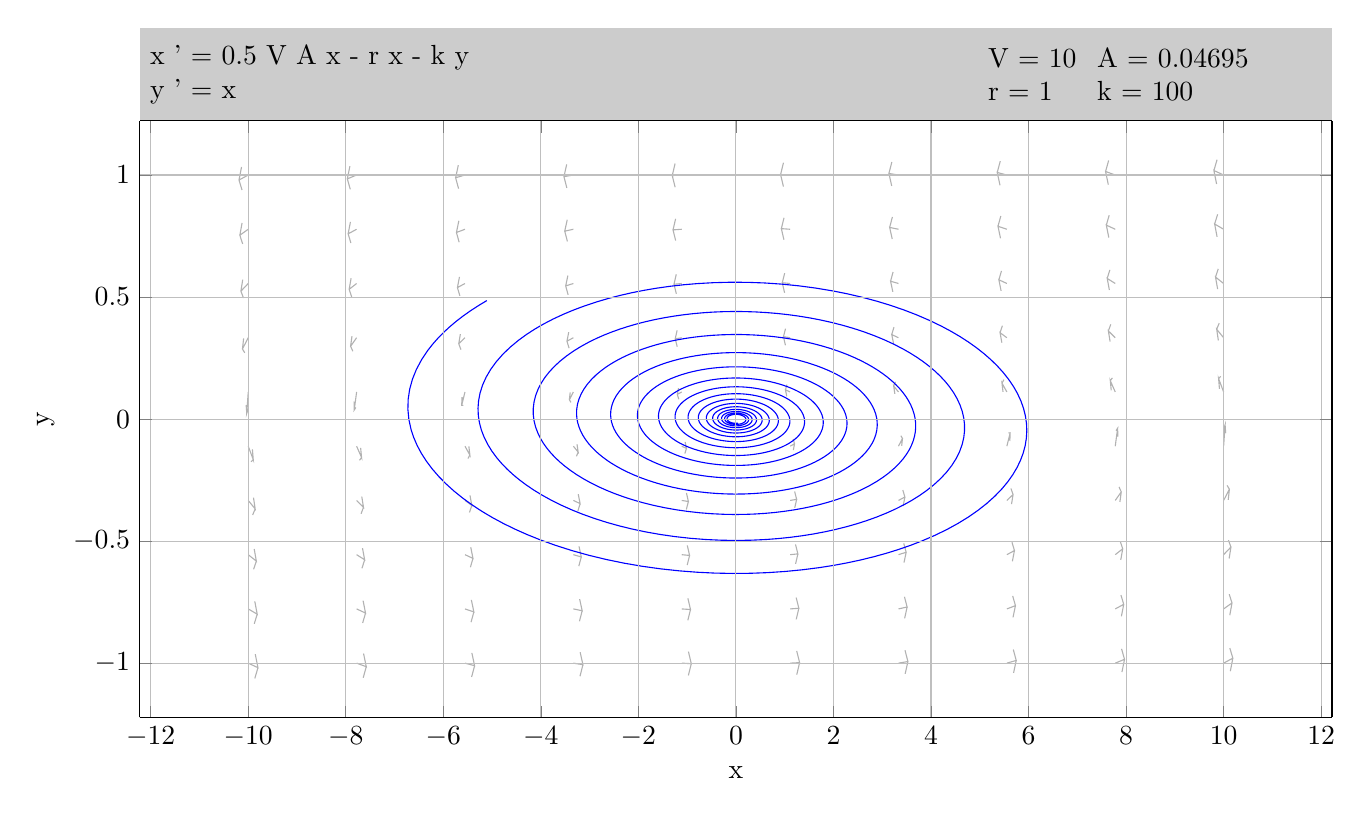
\begin{tikzpicture}

\begin{axis}[%
width=5.960653in,
height=0.465593in,
at={(0.602431in,3.953599in)},
scale only axis,
every outer x axis line/.append style={black},
every x tick label/.append style={font=\color{black}},
xmin=0,
xmax=1,
xtick={-1},
xticklabels={\empty},
every outer y axis line/.append style={black},
every y tick label/.append style={font=\color{black}},
ymin=0,
ymax=1,
ytick={-1},
yticklabels={\empty},
hide axis,
axis background/.style={fill=white!80!black},
axis x line*=bottom,
axis y line*=left
]
\node[right, align=left, inner sep=0mm, text=black]
at (axis cs:0.00806451612903225,0.495614035087719,0) {x ' = 0.5 V A x - r x - k y\\y ' = x};
\node[right, align=left, inner sep=0mm, text=black]
at (axis cs:0.80260034904014,0.5,0) {A = 0.04695\\k = 100};
\node[right, align=left, inner sep=0mm, text=black]
at (axis cs:0.711047120418848,0.5,0) {V = 10\\r = 1};
\node[right, align=left, inner sep=0mm, text=black]
at (axis cs:0.680575916230367,0.5,0) { \\ };
\end{axis}

\begin{axis}[%
width=5.960653in,
height=2.982955in,
at={(0.602431in,0.970644in)},
scale only axis,
unbounded coords=jump,
separate axis lines,
every outer x axis line/.append style={black},
every x tick label/.append style={font=\color{black}},
xmin=-12.2222222222222,
xmax=12.2222222222222,
xlabel={x},
xmajorgrids,
every outer y axis line/.append style={black},
every y tick label/.append style={font=\color{black}},
ymin=-1.22222222222222,
ymax=1.22222222222222,
ylabel={y},
ymajorgrids,
every outer z axis line/.append style={black},
every z tick label/.append style={font=\color{black}},
zmin=-1,
zmax=1,
view={0}{90}
]
\addplot [color=white!70!black,solid,forget plot]
  table[row sep=crcr]{%
-10	-1\\
-9.80085733830155	-1.01849865648252\\
-9.85597547269046	-0.963163394113152\\
-9.80085733830155	-1.01849865648252\\
-9.86522480093172	-1.06273472496238\\
nan	0\\
-10	-0.777777777777778\\
-9.81593667390754	-0.799323221721112\\
-9.86576931074945	-0.746843757014997\\
-9.81593667390754	-0.799323221721112\\
-9.87654203272111	-0.838875420061227\\
nan	0\\
-10	-0.555555555555556\\
-9.83413857553866	-0.581796107175683\\
-9.87733686497203	-0.532458585574309\\
-9.83413857553866	-0.581796107175683\\
-9.89045714078209	-0.615389297804981\\
nan	0\\
-10	-0.333333333333333\\
-9.85801570992342	-0.367975617881226\\
-9.89195042580942	-0.322086859997712\\
-9.85801570992342	-0.367975617881226\\
-9.90927156808337	-0.393079005036003\\
nan	0\\
-10	-0.111111111111111\\
-9.89736072072425	-0.165812351009958\\
-9.91447719453226	-0.123742159221365\\
-9.89736072072425	-0.165812351009958\\
-9.94182781448168	-0.175061798859242\\
nan	0\\
-10	0.111111111111111\\
-10.0301262392884	0.0240060902788186\\
-9.99931211229382	0.0426060367064031\\
-10.0301262392884	0.0240060902788186\\
-10.04286462271	0.0576691563506097\\
nan	0\\
-10	0.333333333333333\\
-10.1181677377517	0.287319352315698\\
-10.0712139211718	0.271581612183062\\
-10.1181677377517	0.287319352315698\\
-10.0942209116806	0.330665481058915\\
nan	0\\
-10	0.555555555555555\\
-10.1503186059397	0.524175802386072\\
-10.0973780858654	0.496010076851982\\
-10.1503186059397	0.524175802386072\\
-10.1130679624502	0.571169379821852\\
nan	0\\
-10	0.777777777777778\\
-10.1719665396443	0.753255017213571\\
-10.11424588761	0.71762021047176\\
-10.1719665396443	0.753255017213571\\
-10.1265072678921	0.803603480293906\\
nan	0\\
-10	1\\
-10.1890256779375	0.979531045460079\\
-10.1272007359213	0.93841531233767\\
-10.1890256779375	0.979531045460079\\
-10.1374352131913	1.03292815130644\\
nan	0\\
-7.77777777777778	-1\\
-7.57947672473115	-1.01455699120751\\
-7.63532779284326	-0.960614630583598\\
-7.57947672473115	-1.01455699120751\\
-7.64260628844702	-1.05976515710691\\
nan	0\\
-7.77777777777778	-0.777777777777778\\
-7.59463794314153	-0.794789907977842\\
-7.64532686098239	-0.743901310258762\\
-7.59463794314153	-0.794789907977842\\
-7.65383292608242	-0.835471227576884\\
nan	0\\
-7.77777777777778	-0.555555555555556\\
-7.61293133757562	-0.576400801734479\\
-7.65717395809153	-0.528935617830262\\
-7.61293133757562	-0.576400801734479\\
-7.66759658118099	-0.611358837931343\\
nan	0\\
-7.77777777777778	-0.333333333333333\\
-7.63687786457782	-0.361228979635658\\
-7.67217392696222	-0.317635307444971\\
-7.63687786457782	-0.361228979635658\\
-7.68612175011339	-0.388085264044951\\
nan	0\\
-7.77777777777778	-0.111111111111111\\
-7.67628774079875	-0.157372869546534\\
-7.6951693122836	-0.118121832771151\\
-7.67628774079875	-0.157372869546534\\
-7.71830019150132	-0.168866851260663\\
nan	0\\
-7.77777777777778	0.111111111111111\\
-7.82663801493469	0.0374511401643854\\
-7.79356495105093	0.0473340721591751\\
-7.82663801493469	0.0374511401643854\\
-7.8303949365243	0.0717641907376311\\
nan	0\\
-7.77777777777778	0.333333333333333\\
-7.90108409522548	0.298307749364745\\
-7.85533580399902	0.277988845193397\\
-7.90108409522548	0.298307749364745\\
-7.87284859598331	0.339642003917247\\
nan	0\\
-7.77777777777778	0.555555555555555\\
-7.93078844623141	0.531563693870408\\
-7.87888728027403	0.500508585262544\\
-7.93078844623141	0.531563693870408\\
-7.89088321111661	0.577013919489361\\
nan	0\\
-7.77777777777778	0.777777777777778\\
-7.95161361538401	0.758953679929299\\
-7.89475683964002	0.721141949882284\\
-7.95161361538401	0.758953679929299\\
-7.90416888856426	0.808059868685402\\
nan	0\\
-7.77777777777778	1\\
-7.96826387367907	0.984246792611236\\
-7.90717974306149	0.941351230852543\\
-7.96826387367907	0.984246792611236\\
-7.91505634675587	1.03659427880319\\
nan	0\\
-5.55555555555556	-1\\
-5.35815419014757	-1.01051951694798\\
-5.41474472053297	-0.958013320511586\\
-5.35815419014757	-1.01051951694798\\
-5.42000447900696	-1.05671400321558\\
nan	0\\
-5.55555555555556	-0.777777777777778\\
-5.3734204518576	-0.790113166863499\\
-5.42497713569556	-0.740878774213295\\
-5.3734204518576	-0.790113166863499\\
-5.43114483023842	-0.831946326062271\\
nan	0\\
-5.55555555555556	-0.555555555555556\\
-5.39184620995722	-0.570762758880916\\
-5.43715721280538	-0.525273261483723\\
-5.39184620995722	-0.570762758880916\\
-5.44476081446806	-0.607127934282893\\
nan	0\\
-5.55555555555556	-0.333333333333333\\
-5.41593749701676	-0.353970864620247\\
-5.45266353175667	-0.312875090599475\\
-5.41593749701676	-0.353970864620247\\
-5.46298229740013	-0.38268411986887\\
nan	0\\
-5.55555555555556	-0.111111111111111\\
-5.45538001156384	-0.147337688813567\\
-5.47637603033574	-0.111425829504901\\
-5.45538001156384	-0.147337688813567\\
-5.49448931918697	-0.161513601500759\\
nan	0\\
-5.55555555555556	0.111111111111111\\
-5.62298097133213	0.0565045787956028\\
-5.58910171352028	0.0560301845461118\\
-5.62298097133213	0.0565045787956028\\
-5.61640497967803	0.0897428924343988\\
nan	0\\
-5.55555555555556	0.333333333333333\\
-5.68312669437639	0.308963279592307\\
-5.63876283929488	0.284381511009406\\
-5.68312669437639	0.308963279592307\\
-5.6509478661654	0.348167080419824\\
nan	0\\
-5.55555555555556	0.555555555555555\\
-5.71094802531824	0.538728627943797\\
-5.6601235524865	0.504928588786653\\
-5.71094802531824	0.538728627943797\\
-5.66853701629238	0.582624823667996\\
nan	0\\
-5.55555555555556	0.777777777777778\\
-5.73110131532847	0.764513775074824\\
-5.67512158672086	0.72460653594248\\
-5.73110131532847	0.764513775074824\\
-5.68175358807234	0.81237941582894\\
nan	0\\
-5.55555555555556	1\\
-5.7474037320527	0.988868525711301\\
-5.68706641053139	0.944245923873624\\
-5.7474037320527	0.988868525711301\\
-5.69263214767573	1.0401700121222\\
nan	0\\
-3.33333333333333	-1\\
-3.13689469083103	-1.0063850819513\\
-3.19423001309389	-0.955359896740335\\
-3.13689469083103	-1.0063850819513\\
-3.19742255406954	-1.05357921799149\\
nan	0\\
-3.33333333333333	-0.777777777777778\\
-3.15229338473611	-0.785290250444451\\
-3.20472725114861	-0.737776521495144\\
-3.15229338473611	-0.785290250444451\\
-3.20848348748195	-0.828296495793755\\
nan	0\\
-3.33333333333333	-0.555555555555556\\
-3.17090352337923	-0.564873510262436\\
-3.21730297768874	-0.521470671361845\\
-3.17090352337923	-0.564873510262436\\
-3.22196195504218	-0.602685576338898\\
nan	0\\
-3.33333333333333	-0.333333333333333\\
-3.19525552364052	-0.346159585365828\\
-3.23347230354024	-0.307792257332877\\
-3.19525552364052	-0.346159585365828\\
-3.23988542955649	-0.376831162179283\\
nan	0\\
-3.33333333333333	-0.111111111111111\\
-3.23488692502806	-0.135130729671655\\
-3.25841594287951	-0.103313242027175\\
-3.23488692502806	-0.135130729671655\\
-3.27042575215978	-0.152536446179809\\
nan	0\\
-3.33333333333333	0.111111111111111\\
-3.41526626656799	0.0792067985947773\\
-3.38271030846851	0.0682948590410137\\
-3.41526626656799	0.0792067985947773\\
-3.39866246472667	0.109261325658341\\
nan	0\\
-3.33333333333333	0.333333333333333\\
-3.4643964182731	0.319140952928908\\
-3.42152939769006	0.290632895815295\\
-3.4643964182731	0.319140952928908\\
-3.42862558789227	0.356164438285177\\
nan	0\\
-3.33333333333333	0.555555555555555\\
-3.49082836403164	0.545651090186224\\
-3.44110373847981	0.509248672122448\\
-3.49082836403164	0.545651090186224\\
-3.44605597116448	0.587996187471599\\
nan	0\\
-3.33333333333333	0.777777777777778\\
-3.51044231251551	0.769930014342742\\
-3.4553476779021	0.728007098577708\\
-3.51044231251551	0.769930014342742\\
-3.45927155961962	0.816561588168797\\
nan	0\\
-3.33333333333333	1\\
-3.52645165911999	0.993394220036544\\
-3.46686471639313	0.947096372578917\\
-3.52645165911999	0.993394220036544\\
-3.47016760637486	1.04365553547224\\
nan	0\\
-1.11111111111111	-1\\
-0.915703479258799	-1.00215289036115\\
-0.973787546224205	-0.952655115289727\\
-0.915703479258799	-1.00215289036115\\
-0.97486399140478	-1.05035893121588\\
nan	0\\
-1.11111111111111	-0.777777777777778\\
-0.931266677892095	-0.780319200767437\\
-0.984584652110384	-0.734595665565786\\
-0.931266677892095	-0.780319200767437\\
-0.985855363605214	-0.824517882175294\\
nan	0\\
-1.11111111111111	-0.555555555555556\\
-0.950126175880236	-0.558726719594556\\
-0.997628865439748	-0.517529136575137\\
-0.950126175880236	-0.558726719594556\\
-0.999214447459249	-0.598021604190575\\
nan	0\\
-1.11111111111111	-0.333333333333333\\
-0.974908163614003	-0.337760501891922\\
-1.01466225572349	-0.302381614450068\\
-0.974908163614003	-0.337760501891922\\
-1.01687584000278	-0.370483088198622\\
nan	0\\
-1.11111111111111	-0.111111111111111\\
-1.01537330502296	-0.120004337565504\\
-1.04187134023581	-0.093401918107148\\
-1.01537330502296	-0.120004337565504\\
-1.046317953463	-0.141270821151224\\
nan	0\\
-1.11111111111111	0.111111111111111\\
-1.20198517870527	0.10127066414783\\
-1.1722628466862	0.0815042813382742\\
-1.20198517870527	0.10127066414783\\
-1.17718307016784	0.126941315135355\\
nan	0\\
-1.11111111111111	0.333333333333333\\
-1.24501187957901	0.328753141319791\\
-1.20369660103525	0.29665200680688\\
-1.24501187957901	0.328753141319791\\
-1.20598669704202	0.363602391040828\\
nan	0\\
-1.11111111111111	0.555555555555555\\
-1.27046038708885	0.552319035090279\\
-1.22184647417921	0.513452672235427\\
-1.27046038708885	0.552319035090279\\
-1.22346473441185	0.593127310224298\\
nan	0\\
-1.11111111111111	0.777777777777778\\
-1.28964900276676	0.775199045397641\\
-1.23544295217503	0.73133819219777\\
-1.28964900276676	0.775199045397641\\
-1.2367323183651	0.820607138025595\\
nan	0\\
-1.11111111111111	1\\
-1.30541390618613	0.997822565815727\\
-1.24657870911756	0.949900097302254\\
-1.30541390618613	0.997822565815727\\
-1.24766742620969	1.04705149483976\\
nan	0\\
1.11111111111111	-1\\
1.30541390618613	-0.997822565815727\\
1.24657870911756	-0.949900097302254\\
1.30541390618613	-0.997822565815727\\
1.24766742620969	-1.04705149483976\\
nan	0\\
1.11111111111111	-0.777777777777778\\
1.28964900276676	-0.775199045397641\\
1.23544295217503	-0.73133819219777\\
1.28964900276676	-0.775199045397641\\
1.2367323183651	-0.820607138025595\\
nan	0\\
1.11111111111111	-0.555555555555556\\
1.27046038708885	-0.55231903509028\\
1.22184647417921	-0.513452672235427\\
1.27046038708885	-0.55231903509028\\
1.22346473441185	-0.593127310224298\\
nan	0\\
1.11111111111111	-0.333333333333333\\
1.24501187957901	-0.328753141319791\\
1.20369660103525	-0.29665200680688\\
1.24501187957901	-0.328753141319791\\
1.20598669704202	-0.363602391040828\\
nan	0\\
1.11111111111111	-0.111111111111111\\
1.20198517870527	-0.10127066414783\\
1.1722628466862	-0.0815042813382742\\
1.20198517870527	-0.10127066414783\\
1.17718307016784	-0.126941315135355\\
nan	0\\
1.11111111111111	0.111111111111111\\
1.01537330502296	0.120004337565504\\
1.04187134023581	0.093401918107148\\
1.01537330502296	0.120004337565504\\
1.046317953463	0.141270821151224\\
nan	0\\
1.11111111111111	0.333333333333333\\
0.974908163614003	0.337760501891922\\
1.01466225572349	0.302381614450068\\
0.974908163614003	0.337760501891922\\
1.01687584000278	0.370483088198622\\
nan	0\\
1.11111111111111	0.555555555555555\\
0.950126175880236	0.558726719594556\\
0.997628865439748	0.517529136575137\\
0.950126175880236	0.558726719594556\\
0.999214447459249	0.598021604190574\\
nan	0\\
1.11111111111111	0.777777777777778\\
0.931266677892095	0.780319200767437\\
0.984584652110384	0.734595665565785\\
0.931266677892095	0.780319200767437\\
0.985855363605214	0.824517882175294\\
nan	0\\
1.11111111111111	1\\
0.915703479258799	1.00215289036115\\
0.973787546224205	0.952655115289727\\
0.915703479258799	1.00215289036115\\
0.97486399140478	1.05035893121588\\
nan	0\\
3.33333333333333	-1\\
3.52645165911999	-0.993394220036544\\
3.46686471639313	-0.947096372578917\\
3.52645165911999	-0.993394220036544\\
3.47016760637486	-1.04365553547224\\
nan	0\\
3.33333333333333	-0.777777777777778\\
3.51044231251551	-0.769930014342742\\
3.4553476779021	-0.728007098577708\\
3.51044231251551	-0.769930014342742\\
3.45927155961962	-0.816561588168797\\
nan	0\\
3.33333333333333	-0.555555555555556\\
3.49082836403164	-0.545651090186225\\
3.44110373847981	-0.509248672122448\\
3.49082836403164	-0.545651090186225\\
3.44605597116448	-0.5879961874716\\
nan	0\\
3.33333333333333	-0.333333333333333\\
3.4643964182731	-0.319140952928908\\
3.42152939769006	-0.290632895815295\\
3.4643964182731	-0.319140952928908\\
3.42862558789228	-0.356164438285177\\
nan	0\\
3.33333333333333	-0.111111111111111\\
3.41526626656799	-0.0792067985947773\\
3.38271030846851	-0.0682948590410137\\
3.41526626656799	-0.0792067985947773\\
3.39866246472668	-0.109261325658341\\
nan	0\\
3.33333333333333	0.111111111111111\\
3.23488692502806	0.135130729671655\\
3.25841594287951	0.103313242027175\\
3.23488692502806	0.135130729671655\\
3.27042575215978	0.152536446179809\\
nan	0\\
3.33333333333333	0.333333333333333\\
3.19525552364052	0.346159585365828\\
3.23347230354024	0.307792257332876\\
3.19525552364052	0.346159585365828\\
3.23988542955649	0.376831162179282\\
nan	0\\
3.33333333333333	0.555555555555555\\
3.17090352337923	0.564873510262435\\
3.21730297768874	0.521470671361845\\
3.17090352337923	0.564873510262435\\
3.22196195504218	0.602685576338898\\
nan	0\\
3.33333333333333	0.777777777777778\\
3.15229338473611	0.785290250444451\\
3.20472725114861	0.737776521495144\\
3.15229338473611	0.785290250444451\\
3.20848348748195	0.828296495793755\\
nan	0\\
3.33333333333333	1\\
3.13689469083103	1.0063850819513\\
3.19423001309389	0.955359896740335\\
3.13689469083103	1.0063850819513\\
3.19742255406955	1.05357921799149\\
nan	0\\
5.55555555555556	-1\\
5.74740373205271	-0.988868525711301\\
5.68706641053139	-0.944245923873624\\
5.74740373205271	-0.988868525711301\\
5.69263214767574	-1.0401700121222\\
nan	0\\
5.55555555555556	-0.777777777777778\\
5.73110131532848	-0.764513775074824\\
5.67512158672086	-0.724606535942481\\
5.73110131532848	-0.764513775074824\\
5.68175358807234	-0.81237941582894\\
nan	0\\
5.55555555555556	-0.555555555555556\\
5.71094802531824	-0.538728627943797\\
5.6601235524865	-0.504928588786653\\
5.71094802531824	-0.538728627943797\\
5.66853701629238	-0.582624823667996\\
nan	0\\
5.55555555555556	-0.333333333333333\\
5.68312669437639	-0.308963279592307\\
5.63876283929489	-0.284381511009406\\
5.68312669437639	-0.308963279592307\\
5.6509478661654	-0.348167080419824\\
nan	0\\
5.55555555555556	-0.111111111111111\\
5.62298097133213	-0.0565045787956028\\
5.58910171352028	-0.0560301845461118\\
5.62298097133213	-0.0565045787956028\\
5.61640497967804	-0.0897428924343988\\
nan	0\\
5.55555555555556	0.111111111111111\\
5.45538001156384	0.147337688813567\\
5.47637603033574	0.111425829504901\\
5.45538001156384	0.147337688813567\\
5.49448931918697	0.161513601500759\\
nan	0\\
5.55555555555556	0.333333333333333\\
5.41593749701677	0.353970864620247\\
5.45266353175668	0.312875090599475\\
5.41593749701677	0.353970864620247\\
5.46298229740013	0.38268411986887\\
nan	0\\
5.55555555555556	0.555555555555555\\
5.39184620995722	0.570762758880916\\
5.43715721280538	0.525273261483723\\
5.39184620995722	0.570762758880916\\
5.44476081446806	0.607127934282892\\
nan	0\\
5.55555555555556	0.777777777777778\\
5.37342045185761	0.790113166863499\\
5.42497713569556	0.740878774213295\\
5.37342045185761	0.790113166863499\\
5.43114483023842	0.831946326062271\\
nan	0\\
5.55555555555556	1\\
5.35815419014757	1.01051951694798\\
5.41474472053297	0.958013320511586\\
5.35815419014757	1.01051951694798\\
5.42000447900696	1.05671400321558\\
nan	0\\
7.77777777777778	-1\\
7.96826387367907	-0.984246792611236\\
7.90717974306149	-0.941351230852543\\
7.96826387367907	-0.984246792611236\\
7.91505634675587	-1.03659427880319\\
nan	0\\
7.77777777777778	-0.777777777777778\\
7.95161361538401	-0.758953679929299\\
7.89475683964002	-0.721141949882284\\
7.95161361538401	-0.758953679929299\\
7.90416888856426	-0.808059868685402\\
nan	0\\
7.77777777777778	-0.555555555555556\\
7.93078844623141	-0.531563693870409\\
7.87888728027404	-0.500508585262544\\
7.93078844623141	-0.531563693870409\\
7.89088321111661	-0.577013919489361\\
nan	0\\
7.77777777777778	-0.333333333333333\\
7.90108409522548	-0.298307749364746\\
7.85533580399902	-0.277988845193397\\
7.90108409522548	-0.298307749364746\\
7.87284859598332	-0.339642003917247\\
nan	0\\
7.77777777777778	-0.111111111111111\\
7.82663801493469	-0.0374511401643854\\
7.79356495105094	-0.0473340721591751\\
7.82663801493469	-0.0374511401643854\\
7.8303949365243	-0.0717641907376311\\
nan	0\\
7.77777777777778	0.111111111111111\\
7.67628774079875	0.157372869546534\\
7.69516931228361	0.118121832771151\\
7.67628774079875	0.157372869546534\\
7.71830019150132	0.168866851260663\\
nan	0\\
7.77777777777778	0.333333333333333\\
7.63687786457782	0.361228979635658\\
7.67217392696223	0.317635307444971\\
7.63687786457782	0.361228979635658\\
7.68612175011339	0.388085264044951\\
nan	0\\
7.77777777777778	0.555555555555555\\
7.61293133757562	0.576400801734479\\
7.65717395809153	0.528935617830261\\
7.61293133757562	0.576400801734479\\
7.667596581181	0.611358837931343\\
nan	0\\
7.77777777777778	0.777777777777778\\
7.59463794314154	0.794789907977842\\
7.64532686098239	0.743901310258762\\
7.59463794314154	0.794789907977842\\
7.65383292608242	0.835471227576884\\
nan	0\\
7.77777777777778	1\\
7.57947672473115	1.01455699120751\\
7.63532779284327	0.960614630583598\\
7.57947672473115	1.01455699120751\\
7.64260628844702	1.05976515710691\\
nan	0\\
10	-1\\
10.1890256779375	-0.979531045460079\\
10.1272007359213	-0.93841531233767\\
10.1890256779375	-0.979531045460079\\
10.1374352131913	-1.03292815130644\\
nan	0\\
10	-0.777777777777778\\
10.1719665396443	-0.753255017213571\\
10.11424588761	-0.71762021047176\\
10.1719665396443	-0.753255017213571\\
10.1265072678921	-0.803603480293906\\
nan	0\\
10	-0.555555555555556\\
10.1503186059397	-0.524175802386072\\
10.0973780858654	-0.496010076851982\\
10.1503186059397	-0.524175802386072\\
10.1130679624502	-0.571169379821852\\
nan	0\\
10	-0.333333333333333\\
10.1181677377517	-0.287319352315698\\
10.0712139211718	-0.271581612183062\\
10.1181677377517	-0.287319352315698\\
10.0942209116806	-0.330665481058915\\
nan	0\\
10	-0.111111111111111\\
10.0301262392884	-0.0240060902788186\\
9.99931211229382	-0.0426060367064031\\
10.0301262392884	-0.0240060902788186\\
10.04286462271	-0.0576691563506097\\
nan	0\\
10	0.111111111111111\\
9.89736072072425	0.165812351009958\\
9.91447719453226	0.123742159221365\\
9.89736072072425	0.165812351009958\\
9.94182781448168	0.175061798859242\\
nan	0\\
10	0.333333333333333\\
9.85801570992342	0.367975617881226\\
9.89195042580942	0.322086859997712\\
9.85801570992342	0.367975617881226\\
9.90927156808337	0.393079005036003\\
nan	0\\
10	0.555555555555555\\
9.83413857553866	0.581796107175683\\
9.87733686497203	0.532458585574309\\
9.83413857553866	0.581796107175683\\
9.89045714078209	0.615389297804981\\
nan	0\\
10	0.777777777777778\\
9.81593667390754	0.799323221721112\\
9.86576931074945	0.746843757014997\\
9.81593667390754	0.799323221721112\\
9.87654203272111	0.838875420061227\\
nan	0\\
10	1\\
9.80085733830155	1.01849865648252\\
9.85597547269046	0.963163394113152\\
9.80085733830155	1.01849865648252\\
9.86522480093172	1.06273472496238\\
nan	0\\
};
\addplot3 [color=blue,solid]
 table[row sep=crcr] {%
-5.1068376068376	0.48548199767712	0\\
-5.12862539063205	0.482976659340549	0.000489539748953975\\
-5.15028213002644	0.480460687069525	0.00097907949790795\\
-5.17180735513997	0.477934145139633	0.00146861924686193\\
-5.19320059945613	0.475397098049854	0.0019581589958159\\
-5.21446139982272	0.472849610522569	0.00244769874476988\\
-5.23558929645183	0.470291747503558	0.00293723849372385\\
-5.25658383291988	0.467723574161997	0.00342677824267783\\
-5.27744455616759	0.465145155890463	0.0039163179916318\\
-5.43946171985027	0.444156702446767	0.0078326359832636\\
-5.59266627679394	0.422550803101269	0.0117489539748954\\
-5.73684761488538	0.400362650982563	0.0156652719665272\\
-5.87181084738597	0.377628045680153	0.019581589958159\\
-5.99737681293169	0.354383393244454	0.0234979079497908\\
-6.11338207553312	0.330665706186793	0.0274142259414226\\
-6.21967892457542	0.306512603479404	0.0313305439330544\\
-6.31613537481834	0.281962310555434	0.0352468619246862\\
-6.44671526137613	0.242954107693286	0.0413573378150945\\
-6.55269092550141	0.203221650431103	0.0474678137055028\\
-6.63376573680999	0.162919051483325	0.0535782895959111\\
-6.68974403752763	0.122199976248651	0.0596887654863194\\
-6.72053114249002	0.0812176428100372	0.0657992413767277\\
-6.72613333914279	0.0401248219347013	0.071909717267136\\
-6.70665788754149	-0.000926162925882157	0.0780201931575444\\
-6.66231302035162	-0.0417834356359802	0.0841306690479527\\
-6.60741185779486	-0.0751293626481535	0.0891553430248317\\
-6.53607563402009	-0.108158731286936	0.0941800170017108\\
-6.4485473460528	-0.14078832731649	0.0992046909785899\\
-6.34510860142319	-0.172937005545271	0.104229364955469\\
-6.22607961816622	-0.204525689826027	0.109254038932348\\
-6.09181922482159	-0.235477373055795	0.114278712909227\\
-5.94272486043373	-0.265717117175909	0.119303386886106\\
-5.77923257455181	-0.295172053171993	0.124328060862985\\
-5.60288225600675	-0.323607315706251	0.129323398537045\\
-5.41325125422029	-0.351128929386071	0.134318736211105\\
-5.21086717587081	-0.377670769940831	0.139314073885165\\
-4.99628350345739	-0.4031700224244	0.144309411559225\\
-4.77007959529979	-0.427567181215138	0.149304749233285\\
-4.53286068553847	-0.450806050015898	0.154300086907345\\
-4.28525788413455	-0.472833741854023	0.159295424581405\\
-4.02792817686986	-0.493600679081348	0.164290762255465\\
-3.70231002492464	-0.517127175311131	0.170375463570089\\
-3.36452263586937	-0.53863633610001	0.176460164884712\\
-3.01589097966825	-0.558055796044683	0.182544866199336\\
-2.6577588524572	-0.575322398846349	0.18862956751396\\
-2.29148887654381	-0.590382197310702	0.194714268828584\\
-1.91846250040739	-0.603190453347936	0.200798970143208\\
-1.54007999869893	-0.61371163797274	0.206883671457832\\
-1.1577604722411	-0.621919431304305	0.212968372772456\\
-0.794560114016997	-0.627527172493779	0.218711594356587\\
-0.430326145490935	-0.631046156202849	0.224454815940718\\
-0.0662830834430466	-0.632473198281928	0.23019803752485\\
0.296364207444596	-0.631812249033626	0.235941259108981\\
0.656430514587985	-0.629074393212755	0.241684480693112\\
1.01275027750118	-0.624277850026327	0.247427702277243\\
1.3641775877963	-0.617447973133554	0.253170923861374\\
1.70958618918355	-0.608617250645848	0.258914145445506\\
1.99835594169629	-0.59954114404792	0.263808364851477\\
2.28127504492422	-0.58906580581023	0.268702584257449\\
2.55767930774734	-0.577221667061353	0.273596803663421\\
2.82692837813217	-0.564042130268899	0.278491023069392\\
3.08840574313176	-0.549563569239522	0.283385242475364\\
3.34151872888567	-0.533825329118914	0.288279461881336\\
3.58569850062	-0.516869726391805	0.293173681287307\\
3.8204000626474	-0.498742048881968	0.298067900693279\\
4.078354497485	-0.476467856963354	0.30370600827861\\
4.32227594019772	-0.452778174958603	0.309344115863942\\
4.5514342855866	-0.427755195039411	0.314982223449273\\
4.76515855602167	-0.401484217726402	0.320620331034605\\
4.96283690144194	-0.374053651889131	0.326258438619936\\
5.14391659935543	-0.345555014746084	0.331896546205268\\
5.30790405483913	-0.316082931864676	0.337534653790599\\
5.45436480053904	-0.285735137161252	0.343172761375931\\
5.57184976258767	-0.257503077550974	0.34829235938816\\
5.67430737285929	-0.228707417550199	0.353411957400388\\
5.76152219026706	-0.199426683041467	0.358531555412617\\
5.83332229363533	-0.169739684187152	0.363651153424846\\
5.88957928169971	-0.139725515429466	0.368770751437074\\
5.93020827310702	-0.109463555490455	0.373890349449303\\
5.95516790641534	-0.0790334673720051	0.379009947461532\\
5.96446034009395	-0.0485151983558362	0.38412954547376\\
5.95790838210771	-0.0175265528640093	0.389326611203129\\
5.93532784319763	0.0133870372898986	0.394523676932498\\
5.89684144521918	0.0441412941770462	0.399720742661867\\
5.84261413570082	0.0746534922292178	0.404917808391236\\
5.77285308784404	0.104842458238824	0.410114874120605\\
5.68780770052336	0.134628571358899	0.415311939849974\\
5.5877695982863	0.163933763103106	0.420509005579343\\
5.47307263135337	0.192681517345732	0.425706071308712\\
5.35495564753592	0.218565278295692	0.430485954577571\\
5.22505906586103	0.243856648359957	0.43526583784643\\
5.08372454837981	0.268499320215423	0.440045721115289\\
4.93131637582734	0.292439142479976	0.444825604384148\\
4.76822144762277	0.315624119712494	0.449605487653007\\
4.59484928186921	0.338004412412849	0.454385370921866\\
4.41163201535383	0.359532337021904	0.459165254190725\\
4.21902440354781	0.380162365921518	0.463945137459584\\
3.97440210724525	0.403833840779776	0.469721468585896\\
3.71762471346089	0.426057931911765	0.475497799712209\\
3.44961287976901	0.446765298498069	0.481274130838521\\
3.17131134521531	0.465892884239416	0.487050461964834\\
2.8836889303169	0.483383917356682	0.492826793091146\\
2.58773853706236	0.499187910590882	0.498603124217459\\
2.28447714891166	0.51326066120318	0.504379455343771\\
1.97494583079622	0.525564250974882	0.510155786470084\\
1.63444257554065	0.536839024998427	0.516400951590846\\
1.28919072253946	0.545973072630188	0.522646116711608\\
0.940582614341401	0.552939479352598	0.52889128183237\\
0.589999390344506	0.557720542230871	0.535136446953133\\
0.238810986796066	0.560307769913008	0.541381612073895\\
-0.111623863207352	0.560701882629791	0.547626777194657\\
-0.459957629719905	0.558912812194788	0.553871942315419\\
-0.804853985946494	0.554959702004352	0.560117107436181\\
-1.07904819400541	0.550223675728481	0.565143468761201\\
-1.34947525661945	0.544118744059504	0.570169830086221\\
-1.61545773780752	0.53666557568085	0.575196191411241\\
-1.87633811904489	0.527888050992252	0.580222552736261\\
-2.13147879926325	0.51781326210974	0.585248914061281\\
-2.38026209485068	0.506471512865646	0.590275275386301\\
-2.62209023965166	0.493896318808602	0.595301636711321\\
-2.85638538496705	0.480124407203541	0.600327998036341\\
-3.09372114448885	0.464415869075751	0.605606585656027\\
-3.32150631825672	0.447479328503183	0.610885173275714\\
-3.53913462994317	0.429367330068233	0.6161637608954\\
-3.74603692377238	0.41013505229544	0.621442348515086\\
-3.94168116452016	0.389840307651488	0.626720936134772\\
-4.12557243751399	0.368543542545204	0.631999523754458\\
-4.29725294863301	0.346307837327563	0.637278111374144\\
-4.456302024308	0.32319890629168	0.642556698993831\\
-4.62825359040562	0.294713275575493	0.648825410728677\\
-4.78125789840907	0.265207929775698	0.655094122463523\\
-4.91478560322664	0.234805459637459	0.66136283419837\\
-5.02839590628761	0.203629908710493	0.667631545933216\\
-5.12173655554219	0.171806773349068	0.673900257668063\\
-5.19454384546159	0.139463002712004	0.680168969402909\\
-5.24664261703798	0.106726998762674	0.686437681137755\\
-5.27794625778449	0.0737286162690028	0.692706392872602\\
-5.28831758752635	0.043986347722328	0.698334319445696\\
-5.28193810903207	0.0142319916665381	0.70396224601879\\
-5.25889626949184	-0.0154387414926214	0.709590172591885\\
-5.2193333051637	-0.0449318506613525	0.715218099164979\\
-5.16344324137357	-0.0741550440578045	0.720846025738073\\
-5.09147289251523	-0.103017739212074	0.726473952311167\\
-5.00372186205035	-0.131431062966205	0.732101878884261\\
-4.90054254250844	-0.15930785147419	0.737729805457356\\
-4.79919714871573	-0.182912155490011	0.74259574328481\\
-4.68688781833629	-0.205996989767525	0.747461681112264\\
-4.56392285307869	-0.228508954019065	0.752327618939718\\
-4.43063255773156	-0.250396661782743	0.757193556767172\\
-4.28736924016358	-0.271610740422446	0.762059494594626\\
-4.13450721132351	-0.292103831127842	0.76692543242208\\
-3.97244278524018	-0.311830588914376	0.771791370249534\\
-3.80159427902247	-0.330747682623272	0.776657308076989\\
-3.58999251277741	-0.351905749507537	0.782380437198708\\
-3.36758069765988	-0.371822490965822	0.788103566320427\\
-3.13514308888055	-0.390436755390547	0.793826695442147\\
-2.8934855484663	-0.407692714377428	0.799549824563866\\
-2.64343554526022	-0.423539862725484	0.805272953685586\\
-2.3858421549216	-0.437933018437033	0.810996082807305\\
-2.12157605992592	-0.450832322717694	0.816719211929025\\
-1.85152954956488	-0.462203239976387	0.822442341050744\\
-1.54857914975786	-0.472920079158408	0.828743766817496\\
-1.24094050757764	-0.481713726103433	0.835045192584249\\
-0.929878930234633	-0.488557073584732	0.841346618351001\\
-0.616650980954908	-0.493431508562546	0.847648044117754\\
-0.302504478980164	-0.496326912184089	0.853949469884506\\
0.0113215004322627	-0.497241659783549	0.860250895651259\\
0.323596626009393	-0.496182620882084	0.866552321418011\\
0.633099310462617	-0.49316515918783	0.872853747184764\\
0.878000435061175	-0.489353471843669	0.877897086418483\\
1.11973501898746	-0.484314502245433	0.882940425652203\\
1.35769255982194	-0.478065771579003	0.887983764885922\\
1.59128002602756	-0.470627716108128	0.893027104119642\\
1.81992185694972	-0.462023687174427	0.898070443353361\\
2.04305996281633	-0.45227995119739	0.903113782587081\\
2.26015372473776	-0.441425689674372	0.9081571218208\\
2.47067999470684	-0.429492999180601	0.91320046105452\\
2.68147383754194	-0.416019616952687	0.918429196756651\\
2.88411709512605	-0.401465011348679	0.923657932458783\\
3.07807972799534	-0.385873621785614	0.928886668160914\\
3.26286299637586	-0.369292188864571	0.934115403863046\\
3.43799946018357	-0.351769754370672	0.939344139565177\\
3.60305297902433	-0.33335766127308	0.944572875267309\\
3.75761871219392	-0.314109553724999	0.94980161096944\\
3.90132311867798	-0.294081377063677	0.955030346671572\\
4.05804547246098	-0.269253153927542	0.961266619076055\\
4.19829417355314	-0.243497918441134	0.967502891480538\\
4.32158572901273	-0.216921744207643	0.973739163885022\\
4.42751333222827	-0.189632123281112	0.979975436289505\\
4.51574686291849	-0.161737966166444	0.986211708693988\\
4.58603288713234	-0.1333496018194	0.992447981098471\\
4.63819465724901	-0.104578777646596	0.998684253502955\\
4.67213211197789	-0.0755386595055048	1.00492052590744\\
4.6871730814339	-0.0488605276317971	1.01061959067886\\
4.68696560392594	-0.0221393215814939	1.01631865545029\\
4.67157281273192	0.00453665316553074	1.02201772022171\\
4.64110748965372	0.0310805955239674	1.02771678499313\\
4.59573206501723	0.0574072088030715	1.03341584976456\\
4.53565861767234	0.0834327007066633	1.03911491453598\\
4.46114887499295	0.109074783333128	1.0448139793074\\
4.37251421287695	0.134252673175415	1.05051304407883\\
4.28558005836077	0.155400243588161	1.0553970111092\\
4.18876825830854	0.176099425536471	1.06028097813957\\
4.08234796072585	0.196301907710681	1.06516494516994\\
3.96660841634143	0.215961161279329	1.07004891220032\\
3.84185897860719	0.235032439889153	1.07493287923069\\
3.70842910369819	0.253472779665093	1.07981684626106\\
3.56666835051265	0.271240999210287	1.08470081329143\\
3.41694638067195	0.288297699606077	1.08958478032181\\
3.23316147078792	0.307205160238862	1.09526940520281\\
3.0397477333149	0.325041050903353	1.10095403008381\\
2.83737914416728	0.341751229395146	1.10663865496481\\
2.62674908278131	0.357286112721231	1.11232327984581\\
2.4085703321151	0.371600677099988	1.11800790472682\\
2.18357507864862	0.384654457961189	1.12369252960782\\
1.95251491238373	0.396411549945995	1.12937715448882\\
1.71616082684412	0.406840606906962	1.13506177936982\\
1.50202994697295	0.414981570099488	1.1401200432489\\
1.28488746524546	0.422031872182238	1.14517830712798\\
1.06530687158699	0.427977310338032	1.15023657100705\\
0.843860763385272	0.43280674236531	1.15529483488613\\
0.621120845490432	0.436512086678144	1.16035309876521\\
0.397657930214974	0.439088322306226	1.16541136264428\\
0.174041937333792	0.440533488894879	1.17046962652336\\
-0.0491581059158357	0.440848686705048	1.17552789040244\\
-0.26107081870468	0.44010017883535	1.18035085464298\\
-0.471600488662731	0.43833287457477	1.18517381888352\\
-0.680256979864204	0.435554564572497	1.18999678312406\\
-0.886560323761303	0.43177533946081	1.1948197473646\\
-1.09004071918423	0.427007589855076	1.19964271160514\\
-1.29023853234116	0.421266006353752	1.20446567584568\\
-1.48670429681828	0.41456757953838	1.20928864008622\\
-1.67899871357977	0.406931599973595	1.21411160432677\\
-1.86406555932208	0.398506801267538	1.21886614222736\\
-2.04425822624278	0.389213494635659	1.22362068012796\\
-2.21918222626558	0.379075971251699	1.22837521802856\\
-2.38845968551528	0.368120183623544	1.23312975592915\\
-2.55172934431783	0.356373745593226	1.23788429382975\\
-2.70864655720028	0.343865932336923	1.24263883173035\\
-2.85888329289077	0.330627680364955	1.24739336963095\\
-3.00212813431859	0.316691587521793	1.25214790753154\\
-3.17043464808781	0.298396278661551	1.2580737417941\\
-3.32688405981222	0.279138110722435	1.26399957605666\\
-3.47096781684047	0.258989900983064	1.26992541031922\\
-3.6022303497019	0.238026494179386	1.27585124458177\\
-3.72026907210652	0.216324762504674	1.28177707884433\\
-3.82473438094507	0.193963605609533	1.28770291310689\\
-3.91532965628895	0.171023950601896	1.29362874736944\\
-3.99181126139026	0.147588752047021	1.299554581632\\
-4.05733701479878	0.12226192469433	1.30584510465149\\
-4.10654476336995	0.0965731295452774	1.31213562767098\\
-4.13930790853031	0.0706275259439802	1.31842615069046\\
-4.15556938735562	0.0445294343922329	1.32471667370995\\
-4.15534167257087	0.0183823365495097	1.33100719672944\\
-4.13870677255025	-0.00771112476703609	1.33729771974893\\
-4.10581623131717	-0.0336491455825717	1.34358824276841\\
-4.05689112854426	-0.059330760764586	1.3498787657879\\
-4.00632863510315	-0.0796455475024578	1.35491644596103\\
-3.94581512476627	-0.0996809110174434	1.35995412613417\\
-3.87554287119941	-0.119386430904151	1.3649918063073\\
-3.79572696837616	-0.138713172935969	1.37002948648043\\
-3.70660533057785	-0.157613689065068	1.37506716665356\\
-3.6084386923936	-0.176042017422401	1.38010484682669\\
-3.50151060872026	-0.1939536823177	1.38514252699983\\
-3.38612745476248	-0.211305694239481	1.39018020717296\\
-3.25645932992489	-0.228848186339247	1.39546066568158\\
-3.11825250359106	-0.245683784266733	1.40074112419021\\
-2.9719303344605	-0.261767648688108	1.40602158269883\\
-2.81793355879454	-0.277057689115573	1.41130204120745\\
-2.65672029041636	-0.291514563907366	1.41658249971608\\
-2.48876602071095	-0.30510168026776	1.4218629582247\\
-2.31456361862513	-0.317785194247061	1.42714341673333\\
-2.13462333066756	-0.329534010741612	1.43242387524195\\
-1.91418687872162	-0.342233954269456	1.43869489231728\\
-1.68728993141537	-0.353531917158573	1.44496590939261\\
-1.45486984073671	-0.363388792514797	1.45123692646795\\
-1.21786964745495	-0.371772028883155	1.45750794354328\\
-0.977238081120855	-0.378655630247874	1.46377896061861\\
-0.733929560066637	-0.384020156032377	1.47004997769394\\
-0.488904191405938	-0.387852721099283	1.47632099476927\\
-0.243127771033834	-0.390146995750408	1.48259201184461\\
-0.0338997743054653	-0.390886871121909	1.4879337653577\\
0.174576583284884	-0.390511076170121	1.49327551887079\\
0.381701304725127	-0.389025037688247	1.49861727238388\\
0.586886619786445	-0.38643734582614	1.50395902589698\\
0.789556985023292	-0.3827597540903	1.50930077941007\\
0.989149083773389	-0.378007179343877	1.51464253292316\\
1.18511182615773	-0.372197701806671	1.51998428643625\\
1.37690634908058	-0.365352565055127	1.52532603994934\\
1.5453998169757	-0.35833145655239	1.53013005779664\\
1.70971880664392	-0.350510764294747	1.53493407564394\\
1.86949482060453	-0.341911576045549	1.53973809349124\\
2.02437430587255	-0.332556560784991	1.54454211133855\\
2.17401865395863	-0.322469968710109	1.54934612918585\\
2.31810420086916	-0.311677631234784	1.55415014703315\\
2.45632222710618	-0.300206960989739	1.55895416488045\\
2.58837895766742	-0.288086951822539	1.56375818272775\\
2.74056859626795	-0.272484006072443	1.56961206843122\\
2.88271796978375	-0.256019024614908	1.5754659541347\\
3.01437398253206	-0.238752952601617	1.58131983983817\\
3.13512776064757	-0.220748582102849	1.58717372554165\\
3.2446146520824	-0.20207055210748	1.59302761124512\\
3.34251422660608	-0.182785348522982	1.5988814969486\\
3.42855027580556	-0.162961304175427	1.60473538265207\\
3.50249081308523	-0.142668598809479	1.61058926835555\\
3.55655752804266	-0.124786118043309	1.6156545600654\\
3.60131169575641	-0.106653004439314	1.62071985177525\\
3.63667175455391	-0.0883172790381882	1.62578514348509\\
3.66258174229721	-0.0698268842632253	1.63085043519494\\
3.67901129638298	-0.0512296839203187	1.63591572690479\\
3.68595565374251	-0.0325734631979621	1.64098101861464\\
3.68343565084171	-0.0139059286672494	1.64604631032449\\
3.67149772368112	0.00472529171812597	1.65111160203434\\
3.65142278969178	0.022400297503493	1.65593786411193\\
3.62293441695229	0.0399583820806132	1.66076412618952\\
3.58612972433494	0.0573586170683026	1.66559038826711\\
3.54112438949396	0.0745609275413668	1.67041665034471\\
3.48805264886559	0.0915260920306014	1.6752429124223\\
3.42706729766806	0.108215742522791	1.68006917449989\\
3.35833968990156	0.124592364460711	1.68489543657748\\
3.28205973834827	0.140619296743125	1.68972169865507\\
3.19953636083962	0.156065235273523	1.69448680534797\\
3.11006227612221	0.171101580693548	1.69925191204087\\
3.0138673505913	0.18569527289595	1.70401701873378\\
2.91119432010811	0.19981465266999	1.70878212542668\\
2.80229878999994	0.213429461701445	1.71354723211958\\
2.68744923506006	0.226510842572602	1.71831233881248\\
2.5669269995478	0.239031338762261	1.72307744550538\\
2.44102629718848	0.250964894645735	1.72784255219828\\
2.27723922060666	0.264963580451087	1.73377438003941\\
2.10619699572445	0.277969695180693	1.73970620788055\\
1.92854216313945	0.289940897792776	1.74563803572168\\
1.74493070206652	0.300839286893696	1.75156986356281\\
1.55603203033783	0.310631400737952	1.75750169140394\\
1.36252900440281	0.319288217228184	1.76343351924507\\
1.16511791932822	0.326785153915169	1.7693653470862\\
0.964508508798083	0.333102067997824	1.77529717492734\\
0.757826118782758	0.338301763709154	1.78133316629335\\
0.549334372192208	0.342248691102025	1.78736915765937\\
0.339813779382553	0.344933575867809	1.79340514902538\\
0.130035589610196	0.346352037309072	1.7994411403914\\
-0.0792382089681751	0.346504588339566	1.80547713175741\\
-0.28725488929559	0.345396635484238	1.81151312312343\\
-0.49327098541479	0.343038478879223	1.81754911448944\\
-0.696552292468243	0.339445312271847	1.82358510585546\\
-0.8614873191001	0.33556970574551	1.82855868565201\\
-1.02367267019305	0.330880497850901	1.83353226544855\\
-1.1827125499147	0.325392404342119	1.8385058452451\\
-1.33822395449241	0.319121972246148	1.84347942504165\\
-1.48983667221329	0.312087579862862	1.84845300483819\\
-1.63719328342418	0.304309436765022	1.85342658463474\\
-1.77994916053167	0.295809583798277	1.85840016443129\\
-1.91777246800212	0.286611893081165	1.86337374422783\\
-2.06281314480213	0.275757369204333	1.86882582993111\\
-2.20113747875225	0.264130075961303	1.87427791563438\\
-2.33235505971109	0.251768119703623	1.87973000133766\\
-2.45610266873545	0.238711297896353	1.88518208704093\\
-2.57204427808024	0.225001099118062	1.8906341727442\\
-2.67987105119854	0.210680703060834	1.89608625844748\\
-2.77930134274157	0.195794980530262	1.90153834415075\\
-2.8700806985587	0.180390493445448	1.90699042985403\\
-2.96512916524892	0.161746150626927	1.91337805709119\\
-3.04765834191132	0.142533824532136	1.91976568432836\\
-3.1173805956235	0.122835951191274	1.92615331156553\\
-3.17406766828617	0.10273549919186	1.9325409388027\\
-3.21755067662314	0.082315969678735	1.93892856603987\\
-3.24772011218136	0.0616613963540606	1.94531619327704\\
-3.26452584133086	0.0408563454773209	1.9517038205142\\
-3.26797710526481	0.0199859158653206	1.95809144775137\\
-3.26059984565394	0.00247567474386502	1.96345414974623\\
-3.24389838752204	-0.0149704160676117	1.96881685174109\\
-3.21795780427361	-0.0323017502136975	1.97417955373595\\
-3.18288915321829	-0.049468761937972	1.97954225573081\\
-3.13882947557078	-0.0664229260830063	1.98490495772567\\
-3.08594179645089	-0.083116758090363	1.99026765972053\\
-3.02441512488356	-0.0995038140005959	1.99563036171539\\
-2.95446445379878	-0.115538690453251	2.00099306371025\\
-2.88475514145882	-0.129583794251718	2.00580265698894\\
-2.80864180776913	-0.143278416053667	2.01061225026763\\
-2.72632522676161	-0.156591780035413	2.01542184354631\\
-2.63801842138234	-0.169494365612129	2.020231436825\\
-2.54394666349159	-0.181957907437848	2.02504103010369\\
-2.44434747386385	-0.193955395405463	2.02985062338238\\
-2.33947062218779	-0.205461074646729	2.03466021666107\\
-2.22957812706627	-0.21645044553226	2.03946980993976\\
-2.08926457564636	-0.229111650821718	2.04533112832314\\
-1.94241570072404	-0.240931708615979	2.05119244670651\\
-1.7895715908579	-0.251872866195003	2.05705376508989\\
-1.63128485029846	-0.261901080973526	2.06291508347327\\
-1.46812059898813	-0.270986020501054	2.06877640185665\\
-1.30065647256123	-0.279101062461869	2.07463772024003\\
-1.12948262234401	-0.286223294675024	2.0804990386234\\
-0.955201715354593	-0.292333515094347	2.08636035700678\\
-0.770266491410794	-0.297623803406405	2.09249023900928\\
-0.583302589077245	-0.301774496223976	2.09862012101177\\
-0.395033867938972	-0.304774643087853	2.10475000301426\\
-0.20617676897279	-0.306617941948948	2.11087988501676\\
-0.0174403145472977	-0.30730273916829	2.11700976701925\\
0.17047389157712	-0.306832029517029	2.12313964902174\\
0.35687166424829	-0.30521345617643	2.12926953102423\\
0.541066236922259	-0.302459310737881	2.13539941302673\\
0.689213637177985	-0.299382592279436	2.14039961758216\\
0.835078832949463	-0.295570709448846	2.14539982213759\\
0.978301229035848	-0.291036011097355	2.15040002669302\\
1.11853143481439	-0.285792533572302	2.15540023124846\\
1.25543126424043	-0.279856000717122	2.16040043580389\\
1.38867373584739	-0.273243823871345	2.16540064035932\\
1.51794307274682	-0.265975101870596	2.17040084491475\\
1.64293470262832	-0.258070621046597	2.17540104947018\\
1.77234538028272	-0.248878187135439	2.18078258586652\\
1.89610731142728	-0.239004273861211	2.18616412226286\\
2.01387925351786	-0.228480536845864	2.1915456586592\\
2.1253424725773	-0.2173401138848	2.19692719505554\\
2.23020074319543	-0.205617624946872	2.20230873145188\\
2.32818034852909	-0.193349172174386	2.20769026784822\\
2.4190300803021	-0.180572339883099	2.21307180424456\\
2.50252123880527	-0.16732619456222	2.2184533406409\\
2.59114370583469	-0.151176536924008	2.22479181753323\\
2.6689634738962	-0.134498683008639	2.23113029442556\\
2.73570967975507	-0.117363254996097	2.23746877131789\\
2.79116239985462	-0.0998414921534293	2.24380724821023\\
2.83515265031621	-0.0820052508347422	2.25014572510256\\
2.86756238693925	-0.063927004481205	2.25648420199489\\
2.88832450520116	-0.045679843621048	2.26282267888722\\
2.89742284025742	-0.0273374758695626	2.26916115577956\\
2.89590189040104	-0.0114546053422453	2.27464272514346\\
2.88570754978241	0.00439656634201224	2.28012429450737\\
2.86690533902511	0.0201678566817606	2.28560586387128\\
2.83958631430493	0.0358120225338955	2.29108743323519\\
2.8038670673499	0.051282760113658	2.2965690025991\\
2.75988972544029	0.0665347049946344	2.30205057196301\\
2.7078219514086	0.0815234321087562	2.30753214132692\\
2.64785694363955	0.0962054557463006	2.31301371069082\\
2.58853683009104	0.108875715975491	2.31785198032379\\
2.52338837341731	0.121245049033986	2.32269024995675\\
2.45258660947269	0.133285257434918	2.32752851958972\\
2.37631797265707	0.144969258929023	2.33236678922268\\
2.2947802959159	0.156271086504639	2.33720505885565\\
2.20818281074023	0.167165888387712	2.34204332848861\\
2.11674614716666	0.177629928041793	2.34688159812158\\
2.02070233377736	0.187640584168035	2.35171986775454\\
1.89968046507957	0.199027161512258	2.35752691539979\\
1.77280209963794	0.209694321142089	2.36333396304504\\
1.64052628899802	0.21960850317321	2.36914101069029\\
1.50332353449346	0.228739287098116	2.37494805833553\\
1.361675787246	0.237059391786116	2.38075510598078\\
1.21607644816546	0.244544675483331	2.38656215362603\\
1.06703036794979	0.251174135812694	2.39236920127128\\
0.915053847085015	0.256929909773951	2.39817624891653\\
0.750088754018303	0.262095376111722	2.40437824589113\\
0.583020352051665	0.266231472056648	2.41058024286574\\
0.414512197123965	0.269326481847526	2.41678223984035\\
0.245221909606809	0.271373030080085	2.42298423681495\\
0.0758011743045393	0.272368081706995	2.42918623378956\\
-0.093104259545761	0.27231294203786	2.43538823076417\\
-0.260854578274269	0.271213256739221	2.44159022773877\\
-0.42681590377843	0.269079011834559	2.44779222471338\\
-0.559449641837844	0.266601980987697	2.45281377539501\\
-0.690169794645641	0.26346364030107	2.45783532607664\\
-0.818649884227835	0.259674440563676	2.46285687675827\\
-0.944573266286878	0.255246374012126	2.4678784274399\\
-1.06763313020166	0.250192974330641	2.47289997812153\\
-1.18753249902753	0.244529316651054	2.47792152880316\\
-1.30398422949624	0.238272017552808	2.48294307948479\\
-1.41671101201601	0.23143923506296	2.48796463016642\\
-1.53189160192092	0.223585801758714	2.49328997733147\\
-1.64227282178092	0.21513156145732	2.49861532449652\\
-1.74755605260378	0.206103143387361	2.50394067166157\\
-1.84746155379163	0.196528475078981	2.50926601882662\\
-1.94172846314095	0.186436782363889	2.51459136599167\\
-2.03011479684257	0.175858589375356	2.51991671315672\\
-2.11239744948168	0.164825718548216	2.52524206032178\\
-2.18837219403782	0.153371290618868	2.53056740748683\\
-2.2698603416979	0.139321283826761	2.53686780675759\\
-2.34197772534221	0.124786792411955	2.54316820602836\\
-2.40447393408169	0.109828734797313	2.54946860529913\\
-2.45714254794467	0.094508670348406	2.55576900456989\\
-2.49982113787687	0.0788887993735133	2.56206940384066\\
-2.53239126574141	0.0630319631236228	2.56836980311142\\
-2.55477848431878	0.0470016437924306	2.57467020238219\\
-2.56695233730688	0.0308619645163409	2.58097060165296\\
-2.56921017081352	0.0165519036975916	2.58654119793984\\
-2.56350619736587	0.00225104681207066	2.59211179422673\\
-2.54989041099305	-0.0119956111374868	2.59768239051362\\
-2.52843722662971	-0.0261439123175377	2.60325298680051\\
-2.49924548011603	-0.0401505360637307	2.6088235830874\\
-2.46243842819771	-0.0539729988809064	2.61439417937428\\
-2.41816374852598	-0.0675696544430973	2.61996477566117\\
-2.36659353965759	-0.0808996935935282	2.62553537194806\\
-2.31578314543641	-0.0922820399337275	2.63039609853859\\
-2.25970081798571	-0.103404763298323	2.63525682512911\\
-2.19849947143746	-0.114242224735569	2.64011755171964\\
-2.13234250938792	-0.124769774748013	2.64497827831016\\
-2.06140382489766	-0.134963753292494	2.64983900490069\\
-1.98586780049151	-0.144801489780142	2.65469973149122\\
-1.90592930815862	-0.154261303076379	2.65956045808174\\
-1.82179370935243	-0.163322501500919	2.66442118467227\\
-1.71687525438603	-0.173524136358522	2.6701851698781\\
-1.60672609625001	-0.183106264066145	2.67594915508393\\
-1.49173958108772	-0.192039105571284	2.68171314028976\\
-1.37231942029052	-0.200295562193332	2.68747712549559\\
-1.24887969049786	-0.207851215623574	2.69324111070143\\
-1.12184483359721	-0.214684327925191	2.69900509590726\\
-0.991649656724113	-0.220775841533258	2.70476908111309\\
-0.858739332262157	-0.226109379254744	2.71053306631892\\
-0.711863815487442	-0.231026253895515	2.71679186897018\\
-0.562902750470205	-0.235017602401158	2.72305067162144\\
-0.412459680908495	-0.238071555820363	2.7293094742727\\
-0.261133393268024	-0.240180250728735	2.73556827692396\\
-0.109517916782168	-0.241339829228793	2.74182707957522\\
0.0417974765480374	-0.241550438949972	2.74808588222648\\
0.19222827195389	-0.240816233048622	2.75434468487774\\
0.341194711899031	-0.239145370208008	2.760603487529\\
0.459679029647278	-0.237126891296138	2.76564263548565\\
0.576545100718546	-0.234515354978287	2.77068178344231\\
0.691498604743301	-0.231319669613522	2.77572093139897\\
0.804253868162993	-0.227550143078631	2.78076007935563\\
0.914533864230065	-0.223218482768125	2.78579922731229\\
1.02207021300795	-0.21833779559424	2.79083837526894\\
1.12660318137105	-0.212922587986933	2.7958775232256\\
1.2278816830048	-0.206988765893882	2.80091667118226\\
1.33024906056881	-0.200233225401033	2.80619679337382\\
1.42850631026668	-0.192947846397438	2.81147691556538\\
1.52239171248897	-0.185155250116378	2.81675703775694\\
1.61165954490908	-0.176879195777769	2.8220371599485\\
1.69608008248327	-0.16814458058817	2.82731728214006\\
1.77543959745067	-0.158977439740782	2.83259740433162\\
1.84954035933329	-0.149404946415444	2.83787752652318\\
1.91820063493597	-0.139455411778635	2.84315764871474\\
1.99244583503675	-0.127189733868181	2.84942810340111\\
2.05852883964611	-0.114483583328862	2.85569855808748\\
2.11622078705282	-0.10138978757499	2.86196901277384\\
2.16533099973466	-0.0879618048321059	2.86823946746021\\
2.20570698435836	-0.0742537241369758	2.87450992214658\\
2.23723443177967	-0.0603202653375958	2.88078037683294\\
2.25983721704329	-0.0462167790931897	2.88705083151931\\
2.27347739938295	-0.0319992468742093	2.89332128620568\\
2.27808193145195	-0.0191612096506361	2.89896069499021\\
2.27544064488356	-0.0063172648098176	2.90460010377473\\
2.26559150061056	0.00649109865427414	2.91023951255926\\
2.24859539655133	0.0192231330788159	2.91587892134379\\
2.22453616760982	0.0318388321321334	2.92151833012832\\
2.19352058567555	0.0442989308137012	2.92715773891285\\
2.15567835962362	0.056564905454143	2.93279714769737\\
2.1111621353147	0.0685989737152315	2.9384365564819\\
2.0673944438333	0.0787946747366357	2.94331549862304\\
2.01887844174961	0.0887654034392824	2.94819444076419\\
1.96574802273164	0.0984879701437575	2.95307338290533\\
1.90814665833514	0.107940062686146	2.95795232504647\\
1.84622739800357	0.117100246418034	2.96283126718761\\
1.78015286906815	0.125947964206504	2.96771020932875\\
1.71009527674782	0.134463536434138	2.9725891514699\\
1.63623640414927	0.14262816099902	2.97746809361104\\
1.54489971648213	0.151744378887741	2.98319773339811\\
1.44890125731949	0.160324189405379	2.98892737318518\\
1.34858026877554	0.168341192201257	2.99465701297225\\
1.24428531587661	0.175771291945116	3.00038665275932\\
1.13637428656115	0.182592698327112	3.00611629254639\\
1.02521439167976	0.18878592605782	3.01184593233346\\
0.911182164995194	0.19433379486823	3.01757557212053\\
0.79466346318231	0.199221429509749	3.0233052119076\\
0.664051038559664	0.203821127251692	3.02960932137487\\
0.531429603412216	0.207591355303009	3.03591343084213\\
0.397345040110046	0.210520501029561	3.0422175403094\\
0.262339401442141	0.212600616787896	3.04852164977667\\
0.126950910616396	0.213827419925243	3.05482575924394\\
-0.00828603874038536	0.214200292779514	3.06112986871121\\
-0.14284088258249	0.213722282679306	3.06743397817847\\
-0.2761868864453	0.212400101943899	3.07373808764574\\
-0.381864610810135	0.210736711664279	3.07879200533522\\
-0.486163431824722	0.208542655119191	3.08384592302469\\
-0.588818856745474	0.205825575091525	3.08889984071417\\
-0.689574009759209	0.202594379317853	3.09395375840364\\
-0.788179631983152	0.198859240488419	3.09900767609312\\
-0.884394081464936	0.194631596247147	3.10406159378259\\
-0.9779833331826	0.189924149191638	3.10911551147207\\
-1.06872097904459	0.184750866873167	3.11416942916154\\
-1.15962159105124	0.17890666963807	3.11941328925701\\
-1.24697913470532	0.172594940659258	3.12465714935248\\
-1.33056383991329	0.165835053208835	3.12990100944795\\
-1.41015960933534	0.158647379316229	3.13514486954342\\
-1.48556401838539	0.1510532897682	3.14038872963889\\
-1.5565883152311	0.143075154108833	3.14563258973436\\
-1.62305742079383	0.134736340639542	3.15087644982984\\
-1.68480992874871	0.12606121641907	3.15612030992531\\
-1.75201575681263	0.115322166197365	3.16236722765677\\
-1.81208773936009	0.104185126900252	3.16861414538824\\
-1.86481833306856	0.0926961096699755	3.17486106311971\\
-1.91003327829878	0.0809017271746659	3.18110798085118\\
-1.94759159909484	0.068849193608335	3.18735489858265\\
-1.97738560318411	0.0565863246908774	3.19360181631412\\
-1.99934088197726	0.0441615376680707	3.19984873404558\\
-2.01341631056829	0.0316238513115743	3.20609565177705\\
-2.01936741584895	0.0201402522682138	3.21178896678838\\
-2.01876453536098	0.00864108326976576	3.21748228179971\\
-2.01163647392693	-0.00283574428389841	3.22317559681103\\
-1.99803330023071	-0.0142529735029749	3.22886891182236\\
-1.97802634681756	-0.0255740020077274	3.23456222683369\\
-1.95170821009409	-0.0367628819284875	3.24025554184502\\
-1.91919275032822	-0.047784319905654	3.24594885685634\\
-1.88061509164926	-0.0586036770896936	3.25164217186767\\
-1.84272250821923	-0.0677167577082936	3.25653620525781\\
-1.80056682806259	-0.0766340962425032	3.26143023864795\\
-1.75426556365727	-0.0853348006231719	3.2663242720381\\
-1.70394492203683	-0.0937987571219868	3.27121830542824\\
-1.64973980479053	-0.102006630351472	3.27611233881838\\
-1.59179380806324	-0.10993986326499	3.28100637220852\\
-1.53025922255551	-0.117580677156739	3.28590040559866\\
-1.46529703352353	-0.124912071661756	3.2907944389888\\
-1.38550136258332	-0.133042900639825	3.29649693051838\\
-1.30155692910703	-0.140707105053029	3.30219942204797\\
-1.21375792683837	-0.147881288665541	3.30790191357755\\
-1.12240689963998	-0.154544049614488	3.31360440510713\\
-1.02781474149345	-0.160675980409948	3.31930689663671\\
-0.930300696499293	-0.166259667934951	3.32500938816629\\
-0.830192358876962	-0.171279693445476	3.33071187969587\\
-0.727825672964836	-0.175722632570459	3.33641437122545\\
-0.635256671957178	-0.179176358257609	3.34148081340685\\
-0.541417000793125	-0.182157906117944	3.34654725558825\\
-0.446555185376064	-0.184661287610315	3.35161369776965\\
-0.350919275673998	-0.186681841113409	3.35668013995105\\
-0.254756845719559	-0.188216231925754	3.36174658213245\\
-0.158314993609997	-0.189262452265718	3.36681302431384\\
-0.0618403415071884	-0.189819821271505	3.37187946649524\\
0.034420964362372	-0.189888985001159	3.37694590867664\\
0.125906549681971	-0.189501017773064	3.3817832721828\\
0.216761689537086	-0.188671989071326	3.38662063568896\\
0.306773696755186	-0.187405437853406	3.39145799919512\\
0.395734392028266	-0.185705902589038	3.39629536270128\\
0.483440103912842	-0.183578921260226	3.40113272620743\\
0.569691668829957	-0.181031031361243	3.40597008971359\\
0.654294431065172	-0.178069769898636	3.41080745321975\\
0.737058242768579	-0.174703673391219	3.41564481672591\\
0.817225892135604	-0.170970466169273	3.42044742971527\\
0.895219843079707	-0.166857379894057	3.42525004270462\\
0.970865977679669	-0.162375354600753	3.43005265569398\\
1.04399770725993	-0.157536068219408	3.43485526868334\\
1.11445597239058	-0.152351936574936	3.43965788167269\\
1.18208924288739	-0.146836113387115	3.44446049466205\\
1.24675351781177	-0.141002490270586	3.44926310765141\\
1.30831232547079	-0.134865696734858	3.45406572064076\\
1.380116784378	-0.126860615243381	3.46001879055733\\
1.44672042178797	-0.118443275946483	3.46597186047389\\
1.50790522856939	-0.109645756887869	3.47192493039046\\
1.56347654776718	-0.100500995466055	3.47787800030702\\
1.61326307460248	-0.091042788434364	3.48383107022359\\
1.65711685647269	-0.0813057919009287	3.48978414014015\\
1.69491329295143	-0.0713255213286885	3.49573721005672\\
1.72655113578856	-0.0611383515353914	3.50169027997328\\
1.75308075504381	-0.0502464487642502	3.50794817762504\\
1.77264024719259	-0.0392098702764144	3.51420607527681\\
1.78518214272109	-0.0280732766552272	3.52046397292857\\
1.79068821235518	-0.0168809374704944	3.52672187058033\\
1.78916946706034	-0.00567673127848473	3.53297976823209\\
1.78066615804174	0.00549585437807035	3.53923766588385\\
1.76524777674416	0.0165937229699765	3.54549556353561\\
1.74301305485205	0.0275741689815771	3.55175346118737\\
1.72022816290535	0.0363045313526523	3.55679399203489\\
1.69316976300907	0.0449094299236648	3.56183452288241\\
1.66192326476615	0.0533672049665866	3.56687505372994\\
1.62658384668817	0.0616568499179717	3.57191558457746\\
1.58725645619533	0.069758011378956	3.57695611542499\\
1.54405580961652	0.077650989115257	3.58199664627251\\
1.49710639218927	0.0853167360571744	3.58703717712003\\
1.44654245805975	0.0927368582995896	3.59207770796756\\
1.3893417178539	0.100291061248517	3.59740388430954\\
1.32844038012748	0.107530908015059	3.60273006065152\\
1.26402789497972	0.114436804245506	3.6080562369935\\
1.19630128874852	0.120990393070512	3.61338241333549\\
1.12546516401048	0.127174555105103	3.61870858967747\\
1.05173169958086	0.132973408448672	3.62403476601945\\
0.975320650513577	0.138372308684977	3.62936094236143\\
0.896459348101265	0.143357848882148	3.63468711870341\\
0.800292901695716	0.148706758159945	3.6409895540748\\
0.701415152541873	0.153441318107468	3.64729198944619\\
0.600238218212017	0.15754507330746	3.65359442481758\\
0.497176231090386	0.161004455140123	3.65989686018896\\
0.392645338373177	0.163808781783116	3.66619929556035\\
0.287063702068546	0.165950258211554	3.67250173093174\\
0.180851498996609	0.167423976198013	3.67880416630313\\
0.0744309207894391	0.168227914312521	3.68510660167452\\
-0.0147209480575136	0.168385741418101	3.69039499157695\\
-0.103473890023623	0.16807313399768	3.69568338147939\\
-0.191577939096214	0.167292792893925	3.70097177138183\\
-0.278788379058528	0.166048718627647	3.70626016128426\\
-0.364865743489721	0.164346211397804	3.7115485511867\\
-0.449575815764865	0.162191871081498	3.71683694108914\\
-0.532689629054948	0.159593597233976	3.72212533099158\\
-0.613983466326875	0.156560589088633	3.72741372089401\\
-0.686112649021869	0.15343515046495	3.73222056976429\\
-0.756396249714727	0.149967360803181	3.73702741863456\\
-0.824676673621708	0.146166537589969	3.74183426750483\\
-0.890802866113137	0.142042672134831	3.7466411163751\\
-0.954630312713403	0.137606429570162	3.75144796524537\\
-1.01602103910096	0.132869148851233	3.75625481411565\\
-1.07484361110834	0.127842842756192	3.76106166298592\\
-1.13097313472211	0.122540197886062	3.76586851185619\\
-1.19594980206278	0.115680430583276	3.7717624333177\\
-1.25649348955208	0.10845052563613	3.77765635477921\\
-1.31240902404342	0.100877568618234	3.78355027624071\\
-1.36352092807643	0.0929894326034364	3.78944419770222\\
-1.40967341987691	0.0848147781658243	3.79533811916373\\
-1.4507304133569	0.0763830533797216	3.80123204062524\\
-1.48657551811461	0.0677244938196897	3.80712596208674\\
-1.51711203943447	0.0588701225605277	3.81301988354825\\
-1.53906049330809	0.0511246933961229	3.8180873450757\\
-1.55698121262259	0.0432780931351208	3.82315480660315\\
-1.57084261485945	0.0353510922569485	3.8282222681306\\
-1.58062414260993	0.0273644083198306	3.83328972965804\\
-1.58631626357505	0.0193387059607886	3.83835719118549\\
-1.58792047056562	0.011294596895641	3.84342465271294\\
-1.58544928150226	0.00325263991900359	3.84849211424039\\
-1.57892623941533	-0.00476665909571088	3.85355957576784\\
-1.56894304901732	-0.0123859255314111	3.85839942260064\\
-1.55532932420001	-0.0199482058436864	3.86323926943344\\
-1.53813029749308	-0.0274357947709561	3.86807911626624\\
-1.51739920959111	-0.0348313733895998	3.87291896309905\\
-1.49319730935359	-0.0421180091139569	3.87775880993185\\
-1.46559385380493	-0.0492791556963269	3.88259865676465\\
-1.43466610813449	-0.0562986532269694	3.88743850359745\\
-1.4004993456965	-0.0631607281341041	3.89227835043025\\
-1.36302429020818	-0.0698773333448783	3.89713820147392\\
-1.32247537882402	-0.0764044409746444	3.90199805251759\\
-1.27896048474528	-0.0827271444061914	3.90685790356126\\
-1.23259332809437	-0.0888312047104401	3.91171775460493\\
-1.18349347591483	-0.0947030506464426	3.9165776056486\\
-1.13178634217134	-0.100329778661383	3.92143745669227\\
-1.07760318774973	-0.105699152890576	3.92629730773594\\
-1.02108112045697	-0.110799605157468	3.93115715877961\\
-0.948463242335113	-0.116695762701038	3.93714243108467\\
-0.87278610751961	-0.122148350048894	3.94312770338973\\
-0.794338438152909	-0.127139385588273	3.94911297569479\\
-0.713414387414204	-0.131652888582471	3.95509824799984\\
-0.630313539519437	-0.135674879170845	3.9610835203049\\
-0.545340909721287	-0.139193378368818	3.96706879260996\\
-0.458806944309182	-0.14219840806787	3.97305406491502\\
-0.371027520609288	-0.144681991035545	3.97903933722008\\
-0.282729045635878	-0.146630025070209	3.98499700636805\\
-0.19382798540867	-0.148050287836796	3.99095467551603\\
-0.104647766138067	-0.148939887840606	3.99691234466401\\
-0.0155075089496262	-0.149297920085138	4.00287001381199\\
0.0732779701159452	-0.149125466072091	4.00882768295997\\
0.161398160102787	-0.148425593801365	4.01478535210795\\
0.248546855139887	-0.147203357771058	4.02074302125593\\
0.334422154441084	-0.145465798977469	4.02670069040391\\
0.404843612670962	-0.143628971076784	4.03166865037564\\
0.474002235971033	-0.141445373970404	4.03663661034737\\
0.541729972237254	-0.138921728941529	4.04160457031911\\
0.607864428821476	-0.136065529300632	4.04657253029084\\
0.672248872531439	-0.132885040385462	4.05154049026257\\
0.734732229630772	-0.129389299561039	4.0565084502343\\
0.795169085838997	-0.12558811621966	4.06147641020603\\
0.853419686331525	-0.121492071780894	4.06644437017777\\
0.915508164601612	-0.116600978344699	4.07197266382454\\
0.974545471427163	-0.11137493397193	4.07750095747132\\
1.03036075980865	-0.105831481859651	4.08302925111809\\
1.08279576241499	-0.0999889027826359	4.08855754476487\\
1.13170479158355	-0.0938662150933653	4.09408583841165\\
1.17695473932013	-0.0874831747220279	4.09961413205842\\
1.21842507729899	-0.0808602751765201	4.1051424257052\\
1.25600785686283	-0.0740187475424462	4.11067071935197\\
1.2947813597566	-0.0657969629479957	4.11711444418056\\
1.32800696397467	-0.0573428272537165	4.12355816900914\\
1.35556878282464	-0.0486931753500467	4.13000189383773\\
1.37737744896891	-0.039884995185187	4.13644561866631\\
1.39337011442467	-0.0309554277651012	4.1428893434949\\
1.4035104505639	-0.0219417671535156	4.14933306832348\\
1.40778864811338	-0.0128814604719201	4.15577679315207\\
1.40622141715471	-0.00381210789956667	4.16222051798065\\
1.40064567012707	0.00355963497223171	4.16747178519367\\
1.39123889614469	0.0108921984394596	4.17272305240669\\
1.37804206868881	0.0181652485742214	4.17797431961971\\
1.3611062838339	0.0253588921524941	4.18322558683273\\
1.34049276024771	0.0324536766541274	4.18847685404575\\
1.3162728391912	0.0394305902628438	4.19372812125877\\
1.28852798451861	0.0462710618662383	4.19897938847179\\
1.25734978267739	0.0529569610557788	4.20423065568481\\
1.22591347458832	0.0589213361491636	4.20903330457624\\
1.1917703155782	0.0647283139460587	4.21383595346767\\
1.15500953395736	0.0703649146383169	4.2186386023591\\
1.11572545852736	0.0758187088137838	4.22344125125053\\
1.07401751858094	0.0810778174562974	4.22824390014196\\
1.02999024390205	0.0861309119456884	4.23304654903339\\
0.98375326476585	0.0909672140577799	4.23784919792482\\
0.935421311938689	0.0955764959643878	4.24265184681625\\
0.873038416452569	0.100939557728018	4.24858093274419\\
0.80787493598306	0.105924695305305	4.25451001867212\\
0.740175511668684	0.110515685298343	4.26043910460006\\
0.670189961566047	0.114697995190008	4.266368190528\\
0.59817328064984	0.118458783343948	4.27229727645593\\
0.524385640812838	0.121786899004587	4.27822636238387\\
0.4490923908659	0.124672882297126	4.28415544831181\\
0.37256405653797	0.127108964227543	4.29008453423975\\
0.293388875720531	0.129126515580314	4.29614167395633\\
0.21350313232301	0.130662429592319	4.30219881367292\\
0.13320808269295	0.131713036679893	4.3082559533895\\
0.0528014370777096	0.132276564398452	4.31431309310609\\
-0.0274226403755409	0.132353137442496	4.32037023282267\\
-0.107173531619819	0.131944777645609	4.32642737253926\\
-0.18616416470833	0.131055403980455	4.33248451225584\\
-0.264111013794466	0.129690832558785	4.33854165197243\\
-0.327430846311869	0.12821246924263	4.34353857166013\\
-0.389694508612578	0.126420293772875	4.34853549134784\\
-0.45074858691045	0.124319988193142	4.35353241103554\\
-0.510444645203173	0.121917947746067	4.35852933072324\\
-0.568639225272266	0.119221280873299	4.36352625041094\\
-0.625193846683076	0.116237809215503	4.36852317009865\\
-0.679975006784781	0.112976067612359	4.37352008978635\\
-0.73285418071039	0.109445304102561	4.37851700947405\\
-0.788344543166568	0.105288893563815	4.38398000441224\\
-0.841258077024466	0.100836260978008	4.38944299935044\\
-0.891444836133886	0.0961020566204503	4.39490599428863\\
-0.938765350575612	0.0911015811246175	4.40036898922682\\
-0.983090626661409	0.0858507854821491	4.40583198416501\\
-1.02430214693402	0.0803662710428493	4.4112949791032\\
-1.06229187016718	0.0746652895146869	4.41675797404139\\
-1.09696223136558	0.0687657429637951	4.42222096897958\\
-1.13322467769402	0.0616295736216202	4.42861790871774\\
-1.16468909372277	0.0542764613932652	4.4350148484559\\
-1.1912455612605	0.0467380468201945	4.44141178819406\\
-1.21280697807082	0.0390461713924824	4.44780872793222\\
-1.22930905787228	0.0312328775488132	4.45420566767038\\
-1.24071033033837	0.0233304086764814	4.46060260740854\\
-1.2469921410975	0.0153712091113915	4.4669995471467\\
-1.24815865173303	0.0073879241380575	4.47339648688486\\
-1.2451998481282	0.000686551498989817	4.4787703741159\\
-1.23866590625546	-0.00598947409576917	4.48414426134695\\
-1.22858992924217	-0.012620708205075	4.48951814857799\\
-1.2150150181764	-0.0191881097476848	4.49489203580904\\
-1.19799427210697	-0.0256730410022568	4.50026592304008\\
-1.17759078804342	-0.0320572676073507	4.50563981027112\\
-1.15387766095603	-0.0383229585614276	4.51101369750217\\
-1.12693798377581	-0.04445268622285	4.51638758473321\\
-1.10002644242888	-0.0498357195411827	4.52122096520774\\
-1.07064943301242	-0.0550827960166104	4.52605434568226\\
-1.03888515163105	-0.0601820089111213	4.53088772615679\\
-1.00481654712861	-0.0651219426080272	4.53572110663132\\
-0.968531321088168	-0.0698916726119639	4.54055448710584\\
-0.930121927832023	-0.0744807655488907	4.54538786758037\\
-0.889685574421701	-0.078879279166091	4.55022124805489\\
-0.847324220657958	-0.0830777623321719	4.55505462852942\\
-0.793342430891655	-0.0879032107842152	4.56093498809927\\
-0.736865241160226	-0.0924040557806254	4.56681534766913\\
-0.678101620322452	-0.0965658392052123	4.57269570723899\\
-0.61726529926171	-0.100375541814103	4.57857606680884\\
-0.554574770885978	-0.103821583235742	4.5844564263787\\
-0.490253290127829	-0.106893821970891	4.59033678594856\\
-0.424528873944437	-0.10958355539263	4.59621714551841\\
-0.35763430131757	-0.111883519746354	4.60209750508827\\
-0.286952701133107	-0.113858550315836	4.60822344316157\\
-0.215524799475499	-0.11539839838685	4.61434938123486\\
-0.143626657233712	-0.116499061979945	4.62047531930816\\
-0.071531402374755	-0.117158308086904	4.62660125738146\\
0.000490770056318202	-0.117375672670742	4.63272719545476\\
0.0721725979364124	-0.117152460665709	4.63885313352805\\
0.143249752064388	-0.116491745977283	4.64497907160135\\
0.213460836161066	-0.115398371482179	4.65110500967465\\
0.270157575769893	-0.11418441357753	4.65612386359197\\
0.325959139738003	-0.112688109235761	4.66114271750928\\
0.380726604310149	-0.110914314840065	4.6661615714266\\
0.434325433583285	-0.108868538221914	4.67118042534392\\
0.486625479506569	-0.106556938661055	4.67619927926123\\
0.537500981881361	-0.103986326885513	4.68121813317855\\
0.586830568361221	-0.101164165071588	4.68623698709587\\
0.634497254451917	-0.0980985668438613	4.69125584101319\\
0.683941572307296	-0.094527175455006	4.69667183195847\\
0.73118147481104	-0.0906938648786123	4.70208782290376\\
0.7760851367804	-0.0866110662063389	4.70750381384905\\
0.818529604807467	-0.0822917836780663	4.71291980479434\\
0.858400797259173	-0.077749594681897	4.71833579573963\\
0.895593504277292	-0.0729986497541553	4.72375178668492\\
0.930011387778436	-0.0680536725793875	4.72916777763021\\
0.961566981454062	-0.0629299599903614	4.73458376857549\\
0.994883497786563	-0.0567018747905831	4.7409478550785\\
1.0240228467326	-0.0502747779996747	4.7473119415815\\
1.04888325390671	-0.043676084443761	4.7536760280845\\
1.06938273780967	-0.0369334262272324	4.7600401145875\\
1.0854591098285	-0.030074652732745	4.76640420109051\\
1.09706997423645	-0.0231278306212204	4.77276828759351\\
1.10419272819299	-0.016121243831846	4.77913237409651\\
1.10682456174384	-0.00908339358207459	4.78549646059951\\
1.10551265303759	-0.00304355609076576	4.79095503176101\\
1.10092038883515	0.00298032050007819	4.79641360292251\\
1.09307463203944	0.00897009678576483	4.80187217408401\\
1.08201178324176	0.0149079967205473	4.80733074524551\\
1.06777778072178	0.0207766076176241	4.81278931640701\\
1.05042810044754	0.0265588801491395	4.81824788756851\\
1.03002775607548	0.0322381283461829	4.82370645873001\\
1.0066512989504	0.0377980295987897	4.82916502989151\\
0.983417264947483	0.0426314785759914	4.8340215500251\\
0.957954514414134	0.047346748396831	4.83887807015869\\
0.930331769427454	0.0519330184576124	4.84373459029228\\
0.900622120315436	0.0563799057011455	4.84859111042587\\
0.868903025656964	0.0606774646167462	4.85344763055946\\
0.835256312281814	0.0648161872402363	4.85830415069305\\
0.799768175270652	0.0687870031539436	4.86316067082664\\
0.762529177955034	0.0725812794867023	4.86801719096023\\
0.715514495031204	0.0769028368541104	4.87386295798818\\
0.666269465539484	0.0809431822707034	4.87970872501613\\
0.614974423147684	0.0846894582969013	4.88555449204408\\
0.561814023464896	0.0881300459062617	4.89140025907203\\
0.50697724404149	0.091254564485479	4.89724602609997\\
0.450657384369112	0.094053871834385	4.90309179312792\\
0.393052065880688	0.0965200641659482	4.90893756015587\\
0.334363231950423	0.0986464761062745	4.91478332718382\\
0.271407955176689	0.100517693197629	4.92095910289302\\
0.207714492478728	0.101997927198636	4.92713487860223\\
0.143533389708572	0.103083128480737	4.93331065431143\\
0.0791127420517555	0.103770873153022	4.93948643002063\\
0.0146981940273123	0.104060363062233	4.94566220572984\\
-0.0494670605122201	0.103952425792759	4.95183798143904\\
-0.113142278380803	0.103449514666641	4.95801375714825\\
-0.176089167058898	0.102555708743567	4.96418953285745\\
-0.226720052027797	0.101541064794854	4.96922587975034\\
-0.276583427704672	0.10027332415415	4.97426222664323\\
-0.325554144395672	0.0987566782482433	4.97929857353612\\
-0.373510930578677	0.0969959091796655	4.98433492042901\\
-0.420336392903303	0.0949963897266875	4.9893712673219\\
-0.4659170161909	0.0927640833433212	4.99440761421479\\
-0.510143163434547	0.0903055441593188	4.99944396110768\\
-0.552909075799061	0.0876279169801732	5.00448030800057\\
-0.596889987064185	0.0845322984557295	5.00986334592442\\
-0.638965879966958	0.0812049718818329	5.01524638384827\\
-0.679020612238984	0.0776566184225788	5.02062942177213\\
-0.716945654654495	0.0738984248891996	5.02601245969598\\
-0.752640091030352	0.0699420837400641	5.03139549761984\\
-0.786010618226045	0.065799793080678	5.03677853554369\\
-0.81697154614369	0.0614842566636834	5.04216157346755\\
-0.845444797728037	0.0570086838888591	5.0475446113914\\
-0.875701728578888	0.0515490651576011	5.05388617313634\\
-0.90230284330992	0.0459089247484325	5.06022773488129\\
-0.925155286985098	0.0401121773128517	5.06656929662623\\
-0.944183487202186	0.0341829536820763	5.07291085837117\\
-0.959329154092747	0.0281456008670433	5.07925242011611\\
-0.970551280322142	0.0220246820584089	5.08559398186106\\
-0.977826141089532	0.0158449766265488	5.091935543606\\
-0.981147294127874	0.00963148012155739	5.09827710535094\\
-0.980825057501208	0.00421701192817657	5.10379489061728\\
-0.977525492646664	-0.00118760769710232	5.10931267588361\\
-0.971270679356913	-0.00656572528036427	5.11483046114995\\
-0.962091591070209	-0.011901012290957	5.12034824641629\\
-0.950028094870397	-0.0171774651414911	5.12586603168262\\
-0.935128951486904	-0.0223794051878399	5.13138381694896\\
-0.917451815294748	-0.0274914787291394	5.13690160221529\\
-0.897063234314531	-0.0324986570077886	5.14241938748163\\
-0.876853805081919	-0.0368231756545432	5.14729399557969\\
-0.854640185278842	-0.0410443597011886	5.15216860367775\\
-0.830482965877523	-0.0451524387429029	5.15704321177581\\
-0.804446714527623	-0.0491380321298226	5.16191781987387\\
-0.776599975556241	-0.0529921489670426	5.16679242797193\\
-0.74701526996791	-0.056706188114616	5.17166703607\\
-0.715769095444604	-0.0602719381875544	5.17654164416806\\
-0.682941926345731	-0.0636815775558277	5.18141625226612\\
-0.641775949638345	-0.0675393099323851	5.18723860458501\\
-0.59862177969035	-0.0711516973868894	5.19306095690391\\
-0.55363634402032	-0.0745073177915967	5.19888330922281\\
-0.506980460355826	-0.0775958248313151	5.20470566154171\\
-0.458818836633439	-0.0804079480034047	5.2105280138606\\
-0.40932007099873	-0.0829354926177776	5.2163503661795\\
-0.358656651806272	-0.085171339796898	5.2221727184984\\
-0.307004957619632	-0.0871094464757824	5.2279950708173\\
-0.25101326538446	-0.0888430527222198	5.23420626321249\\
-0.194318927061078	-0.0902267917045503	5.24041745560769\\
-0.137147744634778	-0.0912567529923156	5.24662864800289\\
-0.0797234446929082	-0.0919305043295228	5.25283984039808\\
-0.0222676784248738	-0.0922470916346444	5.25905103279328\\
0.0349999783778635	-0.0922070390006187	5.26526222518848\\
0.0918620253217848	-0.0918123486948494	5.27147341758368\\
0.148103037411316	-0.0910665011592057	5.27768460997887\\
0.193229692288648	-0.0902042900488208	5.28273511941178\\
0.237691428691111	-0.0891158151989043	5.28778562884468\\
0.281375937381389	-0.0878047264485891	5.29283613827758\\
0.324174345786632	-0.0862752062766576	5.29788664771048\\
0.365981217998451	-0.0845319698015417	5.30293715714338\\
0.406694554772925	-0.0825802647813231	5.30798766657628\\
0.446215793530594	-0.0804258716137327	5.31303817600918\\
0.484449808356465	-0.0780751033361511	5.31808868544208\\
0.523529834146984	-0.0753720305882431	5.32345046396251\\
0.560949442693135	-0.0724637975611898	5.32881224248294\\
0.59660606984795	-0.0693596795372115	5.33417402100337\\
0.630403758097237	-0.0660693987148361	5.3395357995238\\
0.662253156559579	-0.0626031242089	5.34489757804424\\
0.692071520986338	-0.0589714720505474	5.35025935656467\\
0.719782713761649	-0.0551855051872309	5.3556211350851\\
0.745317203902428	-0.0512567334827107	5.36098291360553\\
0.772565181743437	-0.0464526806524069	5.36731026949117\\
0.796599367241082	-0.0414861805519949	5.37363762537681\\
0.817335898754718	-0.0363782131097219	5.37996498126245\\
0.834706088170735	-0.0311499634976252	5.38629233714809\\
0.848656420902557	-0.0258228221315319	5.39261969303373\\
0.85914855589064	-0.0204183846710588	5.39894704891937\\
0.866159325602477	-0.0149584520196129	5.40527440480501\\
0.869680736032591	-0.00946503032439045	5.41160176069065\\
0.869897650013842	-0.00462929820478276	5.4171597527289\\
0.867433275009146	0.00020032030111947	5.42271774476715\\
0.862306103880534	0.00500871149645949	5.42827573680541\\
0.854542785477483	0.00978105136765474	5.43383372884366\\
0.844178124636918	0.0145028055843968	5.43939172088191\\
0.831255082183209	0.0191597294996515	5.44494971292016\\
0.815824774928172	0.0237378681496586	5.45050770495841\\
0.797946475671071	0.0282235562539326	5.45606569699666\\
0.780247988231484	0.0320823158322811	5.46095471644485\\
0.760754315003199	0.0358502161481396	5.46584373589305\\
0.739519056120558	0.0395184776111519	5.47073275534124\\
0.716599405792429	0.0430786679961737	5.47562177478943\\
0.6920561523022	0.0465227024432721	5.48051079423762\\
0.665953678007786	0.0498428434577261	5.48539981368581\\
0.638359959341627	0.0530317009100261	5.490288833134\\
0.609346566810683	0.0560822320358746	5.4951778525822\\
0.573133941885268	0.059517478998668	5.50098622589427\\
0.53515224966606	0.0627373625308628	5.50679459920635\\
0.495539037271141	0.0657317401644017	5.51260297251842\\
0.454435333859433	0.0684914115069802	5.5184113458305\\
0.411985650630698	0.0710081182420469	5.52421971914258\\
0.36833798082554	0.0732745441288034	5.53002809245465\\
0.323643799725401	0.075284315002204	5.53583646576673\\
0.278058064652562	0.0770319987729564	5.54164483907881\\
0.228309846280792	0.078611144608456	5.5478797026663\\
0.177911167152734	0.0798781731553844	5.55411456625379\\
0.127064414497527	0.0808294327177558	5.56034942984128\\
0.075970190104916	0.0814626041807027	5.56658429342877\\
0.0248273103252488	0.0817767010104754	5.57281915701626\\
-0.0261671939305241	0.0817720692544424	5.57905402060375\\
-0.076818077190848	0.0814503875410903	5.58528888419124\\
-0.126931879423567	0.0808146670800234	5.59152374777874\\
-0.167092313086968	0.0800702603610469	5.59658578563427\\
-0.206671117045169	0.079124005600084	5.60164782348981\\
-0.245567809522637	0.0779791076149083	5.60670986134535\\
-0.283684961999293	0.0766392494365918	5.61177189920089\\
-0.320928199210509	0.0751085923095045	5.61683393705642\\
-0.357206199147111	0.0733917756913148	5.62189597491196\\
-0.392430693055377	0.0714939172529894	5.6269580127675\\
-0.426516465437039	0.0694206128787931	5.63202005062304\\
-0.461217984146214	0.0670448902042645	5.63737081767984\\
-0.494461304884482	0.0644873249116652	5.64272158473664\\
-0.526155637844185	0.0617560472424776	5.64807235179343\\
-0.556215983900163	0.0588595833079599	5.65342311885023\\
-0.584563134609758	0.0558068550891458	5.65877388590703\\
-0.611123672212809	0.052607180436845	5.66412465296383\\
-0.635829969631656	0.0492702730716427	5.66947542002063\\
-0.658620190471139	0.0458062425838996	5.67482618707743\\
-0.682995738947614	0.041564824542439	5.68114646102675\\
-0.70453493622166	0.037178127625213	5.68746673497607\\
-0.723162623695933	0.0326646491765269	5.69378700892539\\
-0.73881702929198	0.0280430753814368	5.70010728287471\\
-0.751449767450244	0.0233322812657499	5.70642755682403\\
-0.761025839130064	0.0185513306960246	5.71274783077335\\
-0.767523631809672	0.0137194763795703	5.71906810472267\\
-0.770934919486194	0.00885615986444728	5.72538837867199\\
-0.771382100451296	0.00454958182556707	5.73097124205372\\
-0.769429282206676	0.000247086919485055	5.73655410543546\\
-0.765092314167843	-0.0040377325397446	5.7421369688172\\
-0.758394426819506	-0.00829154224697187	5.74771983219893\\
-0.749366231715568	-0.0125012659059509	5.75330269558067\\
-0.738045721479132	-0.0166540852293398	5.75888555896241\\
-0.724478269802493	-0.020737439938701	5.76446842234415\\
-0.708716631447149	-0.0247390277645011	5.77005128572588\\
-0.693118749553707	-0.0281746971805799	5.77495187581405\\
-0.675917997537358	-0.031530051923694	5.77985246590222\\
-0.657161950086267	-0.0347972332329364	5.78475305599039\\
-0.636901411189491	-0.0379686922122095	5.78965364607856\\
-0.61519041413697	-0.0410371898302251	5.79455423616672\\
-0.592086221519533	-0.0439957969205044	5.79945482625489\\
-0.567649325228897	-0.0468378941813782	5.80435541634306\\
-0.541943446457666	-0.0495571721759866	5.80925600643123\\
-0.509954544386022	-0.0526100976300405	5.81505875060392\\
-0.476393753531106	-0.0554729369412437	5.82086149477661\\
-0.441382416210714	-0.0581366852485885	5.8266642389493\\
-0.405044978440706	-0.0605931686081976	5.832466983122\\
-0.367508989935008	-0.0628350439933235	5.83826972729469\\
-0.328905104105606	-0.064855799294349	5.84407247146738\\
-0.289367078062556	-0.0666497533187868	5.84987521564007\\
-0.249031772613973	-0.0682120557912799	5.85567795981277\\
-0.204864025109518	-0.0696306509023384	5.86192640644482\\
-0.160107374613563	-0.0707715026139748	5.86817485307688\\
-0.114942391573416	-0.0716312902340043	5.87442329970894\\
-0.0695480840966683	-0.0722078857602798	5.880671746341\\
-0.0241018979511936	-0.0725003538806916	5.88692019297305\\
0.0212202834348496	-0.0725089519731681	5.89316863960511\\
0.0662441389730193	-0.072235130105675	5.89941708623717\\
0.110796909914591	-0.0716815310362159	5.90566553286923\\
0.146493382255348	-0.0710289200857657	5.91073693810134\\
0.181676420068049	-0.0701965563418649	5.91580834333344\\
0.216256348835933	-0.0691872762167819	5.92087974856555\\
0.250146213565677	-0.0680043439054795	5.92595115379766\\
0.283261778787397	-0.0666514513856152	5.93102255902977\\
0.315521528554648	-0.065132718417541	5.93609396426188\\
0.346846666444425	-0.0634526925443034	5.94116536949398\\
0.37716111555716	-0.0616163490916431	5.94623677472609\\
0.407959597554432	-0.0595159094179656	5.95158583154507\\
0.437468624715661	-0.0572541189303321	5.95693488836404\\
0.465607640777076	-0.0548381653099049	5.96228394518301\\
0.492301211418317	-0.0522755876940231	5.96763300200199\\
0.517479024262445	-0.0495742766762032	5.97298205882096\\
0.541075888875934	-0.0467424743061386	5.97833111563994\\
0.563031736768673	-0.0437887740897	5.98368017245891\\
0.583291621393971	-0.0407221209889349	5.98902922927789\\
0.604974610859083	-0.0369659196465288	5.99534880865625\\
0.624145356334632	-0.0330804680193346	6.00166838803462\\
0.640736926385397	-0.0290821487959866	6.00798796741298\\
0.654694251810352	-0.0249875142584535	6.01430754679135\\
0.665974125642666	-0.0208132862820381	6.02062712616971\\
0.674545203149707	-0.0165763563353775	6.02694670554807\\
0.680388001833038	-0.0122937854804433	6.03326628492644\\
0.683494901428418	-0.00798280437254078	6.0395858643048\\
0.683963118118114	-0.00415645347417137	6.04518045711872\\
0.682294085767486	-0.000333354321296895	6.05077504993263\\
0.678501733976272	0.00347436214378059	6.05636964274655\\
0.672606597399415	0.00725479481797768	6.06196423556046\\
0.664635815747065	0.0109962724374296	6.06755882837437\\
0.654623133784582	0.0146873535774904	6.07315342118829\\
0.642608901332531	0.0183168266527325	6.0787480140022\\
0.628640073266687	0.0218737099169472	6.08434260681611\\
0.614811325931172	0.0249269840711205	6.0892524836059\\
0.599555286750327	0.0279089031828973	6.09416236039568\\
0.582914322715483	0.0308124556852847	6.09907223718547\\
0.564933687917604	0.0336309067373429	6.10398211397525\\
0.54566152354729	0.0363577982241846	6.10889199076504\\
0.525148857894776	0.0389869487569757	6.11380186755482\\
0.50344960634993	0.0415124536729345	6.11871174434461\\
0.480620571402256	0.0439286850353324	6.12362162113439\\
0.4522533470796	0.0466371065540439	6.12942637800859\\
0.422491073587074	0.0491769012861829	6.13523113488278\\
0.391441437072787	0.0515400745021612	6.14103589175698\\
0.359214880554721	0.0537193692180263	6.14684064863117\\
0.32592460392074	0.0557082661954604	6.15264540550536\\
0.291686563928581	0.0575009839417811	6.15845016237956\\
0.256619474205863	0.0590924787099411	6.16425491925375\\
0.220844805250078	0.0604784444985283	6.17005967612795\\
0.181655533275747	0.0617373277092775	6.17631267890072\\
0.141943293473007	0.0627495932630327	6.18256568167349\\
0.101868542289997	0.0635122900848285	6.18881868444626\\
0.0615903453947524	0.0640235277717409	6.19507168721903\\
0.0212663776752023	0.0642824765928877	6.2013246899918\\
-0.0189470767608285	0.064289367489428	6.20757769276457\\
-0.0588951245856199	0.0640454920745624	6.21383069553734\\
-0.0984242632515575	0.0635532026335332	6.22008369831011\\
-0.130118776805719	0.062972644478894	6.22516265813374\\
-0.161356119322213	0.0622322512906099	6.23024161795738\\
-0.192056434649338	0.0613345524369038	6.23532057778101\\
-0.222142295024656	0.0602824587405965	6.24039953760464\\
-0.251538701074992	0.0590792624791071	6.24547849742828\\
-0.280173081816429	0.0577286373844527	6.25055745725191\\
-0.307975294654315	0.0562346386432485	6.25563641707554\\
-0.334877625383257	0.0546017028967077	6.26071537689917\\
-0.36220088210787	0.052734388096465	6.26607135693356\\
-0.388376585461334	0.050723753086827	6.27142733696795\\
-0.413333098769952	0.0485762028675067	6.27678331700234\\
-0.437003354309489	0.0462984551577177	6.28213929703672\\
-0.459324853305171	0.0438975403961733	6.28749527707111\\
-0.480239665931686	0.0413808017410874	6.2928512571055\\
-0.499694431313183	0.0387558950701738	6.29820723713988\\
-0.517640357523271	0.0360307889806466	6.30356321717427\\
-0.536829815351981	0.0326947665247947	6.30988802609704\\
-0.553786650065113	0.0292442914099946	6.31621283501981\\
-0.568451595135371	0.0256939347942782	6.32253764394258\\
-0.580775938902986	0.0220584169490723	6.32886245286535\\
-0.590721524575719	0.0183526072591973	6.33518726178812\\
-0.598260750228861	0.0145915242228682	6.34151207071089\\
-0.603376568805231	0.0107903354516943	6.34783687963366\\
-0.606062488115177	0.00696435767067856	6.35416168855643\\
-0.606414010671782	0.00357171243559517	6.35975620844923\\
-0.604870928807851	0.00018230518499698	6.36535072834203\\
-0.601445792294754	-0.00319311098973511	6.37094524823483\\
-0.596157002273684	-0.00654398786718555	6.37653976812763\\
-0.589028811255666	-0.00985998209590416	6.38213428802043\\
-0.580091323121552	-0.0131309551944062	6.38772880791323\\
-0.569380493122022	-0.016346973551172	6.39332332780604\\
-0.556938127877587	-0.0194983084246478	6.39891784769884\\
-0.544608598314697	-0.0222072209034696	6.40383513222753\\
-0.53101116896358	-0.0248524296214716	6.40875241675621\\
-0.516183692737996	-0.0274276968065836	6.4136697012849\\
-0.500166592305687	-0.0299270321356374	6.41858698581359\\
-0.483002860088378	-0.0323446927343663	6.42350427034228\\
-0.46473805826178	-0.0346751831774056	6.42842155487097\\
-0.445420318755586	-0.0369132554882922	6.43333883939966\\
-0.425100343253475	-0.0390539091394649	6.43825612392835\\
-0.399853579373144	-0.0414527910526528	6.444070048491\\
-0.373370063781761	-0.0437013726925021	6.44988397305366\\
-0.345745897561355	-0.0457925562118995	6.45569789761631\\
-0.317079622678885	-0.0477199028580711	6.46151182217897\\
-0.287472221986237	-0.0494776329725827	6.46732574674162\\
-0.257027119220232	-0.0510606259913398	6.47313967130428\\
-0.225850179002616	-0.0524644204445873	6.47895359586693\\
-0.194049706840068	-0.0536852139569101	6.48476752042959\\
-0.159296858252345	-0.0547896934972306	6.49101675204702\\
-0.124087890753328	-0.0556756288035594	6.49726598366446\\
-0.088564859370721	-0.0563404528816448	6.50351521528189\\
-0.0528685609321922	-0.0567825364541431	6.50976444689932\\
-0.0171385340653784	-0.0570011879606182	6.51601367851676\\
0.018486940802117	-0.0569966535575421	6.52226291013419\\
0.0538708414427239	-0.0567701171182948	6.52851214175162\\
0.0888774038289059	-0.0563237002331639	6.53476137336906\\
0.116991054797078	-0.0558001214540893	6.53984635538533\\
0.144694297573195	-0.0551346100508572	6.5449313374016\\
0.171916156941861	-0.0543294378040518	6.55001631941786\\
0.198587831554188	-0.0533872156675431	6.55510130143413\\
0.224642693927805	-0.0523108937684868	6.5601862834504\\
0.250016290446848	-0.0511037614073243	6.56527126546667\\
0.27464634136197	-0.0497694470577827	6.57035624748294\\
0.298472740790332	-0.0483119183668749	6.57544122949921\\
0.322702990004321	-0.0466432549855081	6.58081224814785\\
0.345905831679999	-0.0448471641678447	6.58618326679649\\
0.368017429362827	-0.0429293960438844	6.59155428544514\\
0.388978054690788	-0.0408959795583393	6.59692530409378\\
0.408732087394392	-0.0387532224706337	6.60229632274242\\
0.427228015296672	-0.0365077113549039	6.60766734139107\\
0.444418434313184	-0.0341663115999988	6.61303836003971\\
0.460260048452009	-0.0317361674094793	6.61840937868836\\
0.477160082946047	-0.0287653600664604	6.624745044983\\
0.492069744185914	-0.0256936563768516	6.63108071127764\\
0.504936838611489	-0.0225340679238823	6.63741637757228\\
0.515718600788603	-0.0192997346925107	6.64375204386692\\
0.524381693409043	-0.0160039250694247	6.65008771016155\\
0.530902207290546	-0.012660035843041	6.65642337645619\\
0.535265661376801	-0.00928159220350605	6.66275904275083\\
0.537467002737453	-0.00588224774269508	6.66909470904547\\
0.537616128297273	-0.00287999577338724	6.67467816911293\\
0.536092901321117	0.000118503568914471	6.68026162918039\\
0.532908881423738	0.0031037791133291	6.68584508924785\\
0.528080763299976	0.00606654240293329	6.69142854931531\\
0.52163037672476	0.00899768769476132	6.69701200938277\\
0.513584686553101	0.0118882919598051	6.70259546945023\\
0.503975792720098	0.0147296148830141	6.70817892951768\\
0.492840930240937	0.0175130988632955	6.71376238958514\\
0.481789593562677	0.0199127541479898	6.71868552638989\\
0.469614427317646	0.0222552725981007	6.72360866319464\\
0.456349359478462	0.0245351192574801	6.7285317999994\\
0.442030596057077	0.026746980746165	6.73345493680415\\
0.426696621104773	0.0288857652603775	6.7383780736089\\
0.410388196712166	0.0309466025725252	6.74330121041365\\
0.393148363009205	0.0329248440312003	6.7482243472184\\
0.37502243816517	0.0348160625611807	6.75314748402315\\
0.35247618157526	0.0369373666169206	6.75897737009719\\
0.32883473715543	0.0389241058404239	6.76480725617123\\
0.304184319196584	0.0407699792929837	6.77063714224527\\
0.278613295881628	0.0424692783128713	6.77646702831931\\
0.252212189285476	0.0440168865153362	6.78229691439335\\
0.225073675375046	0.0454082797926061	6.78812680046739\\
0.197292584009259	0.0466395263138868	6.79395668654143\\
0.168965898939043	0.0477072865253623	6.79978657261547\\
0.138163967645648	0.0486655160623285	6.80602418536196\\
0.106971275059787	0.0494304475972725	6.81226179810846\\
0.0755131421841358	0.0499998953395748	6.81849941085495\\
0.0439137356248628	0.0503724978832509	6.82473702360145\\
0.0122960675916269	0.0505477182069517	6.83097463634794\\
-0.0192180041024213	0.0505258436739632	6.83721224909444\\
-0.0505077760406391	0.0503079860322063	6.84344986184093\\
-0.0814536992028935	0.0498960814142376	6.84968747458743\\
-0.106368010568451	0.0494179558510513	6.8547771949316\\
-0.130911078164015	0.0488139513426158	6.85986691527576\\
-0.155019931474583	0.0480861221025746	6.86495663561993\\
-0.178633550852778	0.0472368231336117	6.8700463559641\\
-0.201692867518848	0.0462687102274523	6.87513607630826\\
-0.224140763560667	0.0451847399648618	6.88022579665243\\
-0.245922071933731	0.0439881697156465	6.88531551699659\\
-0.266983576461166	0.0426825576386535	6.89040523734076\\
-0.288460796632732	0.041184156841819	6.89579896206976\\
-0.309012985354808	0.0395723673497353	6.90119268679875\\
-0.328583153388711	0.0378523875090227	6.90658641152775\\
-0.347118032723258	0.0360296646726675	6.91198013625675\\
-0.364568076574774	0.0341098952000219	6.91737386098574\\
-0.380887459387084	0.0320990244568042	6.92276758571474\\
-0.396034076831519	0.0300032468150985	6.92816131044374\\
-0.409969545806913	0.0278290056533549	6.93355503517273\\
-0.424781126285449	0.0251767631775036	6.93990699196709\\
-0.437813028519621	0.022435974578463	6.94625894876145\\
-0.449019542829122	0.019618302631868	6.95261090555581\\
-0.458363412245342	0.0167355181917146	6.95896286235017\\
-0.46581583251137	0.0137995001903594	6.96531481914453\\
-0.471356452081988	0.0108222356385201	6.97166677593889\\
-0.474973372123681	0.00781581962527516	6.97801873273325\\
-0.476663146514625	0.00479245531806402	6.98437068952761\\
-0.476562349486665	0.00214079051814768	6.98993258078108\\
-0.474991510702535	-0.000506298140913563	6.99549447203455\\
-0.471961468040396	-0.00314052003386248	7.00105636328802\\
-0.467487524976724	-0.00575374750800119	7.00661825454149\\
-0.461589450586303	-0.00833801588319114	7.01218014579496\\
-0.454291479542232	-0.0108855234518531	7.01774203704843\\
-0.44562231211592	-0.0133886314789673	7.0233039283019\\
-0.435615114177087	-0.0158398642020731	7.02886581955538\\
-0.425660300053382	-0.0179623999882817	7.03379353772457\\
-0.414711418846311	-0.0200334646361794	7.03872125589376\\
-0.402798974581816	-0.0220481586415258	7.04364897406296\\
-0.389955483080791	-0.0240017811975927	7.04857669223215\\
-0.376215471959088	-0.0258898301951641	7.05350441040135\\
-0.36161548062751	-0.0277080022225358	7.05843212857054\\
-0.346194060291817	-0.0294521925655161	7.06335984673973\\
-0.32999177395272	-0.031118495207425	7.06828756490893\\
-0.309792535027709	-0.0329912264796242	7.07413991009786\\
-0.288624667062685	-0.034742973214196	7.07999225528679\\
-0.266565899132306	-0.0363681434777781	7.08584460047572\\
-0.243695853827051	-0.0378616805071953	7.09169694566465\\
-0.220096047253214	-0.0392190627094589	7.09754929085358\\
-0.19584988903291	-0.0404363036617672	7.10340163604251\\
-0.17104268230407	-0.0415099521115052	7.10925398123144\\
-0.145761623720443	-0.0424370919762448	7.11510632642037\\
-0.118477227276885	-0.0432589738514066	7.1213248230672\\
-0.0908642814709974	-0.0439102095259075	7.12754331971404\\
-0.063032964453966	-0.0443889791967242	7.13376181636087\\
-0.0350923832045267	-0.0446941838854003	7.1399803130077\\
-0.00715057352896628	-0.044825445438047	7.14619880965454\\
0.0206854999388779	-0.0447831065253428	7.15241730630137\\
0.0483099437376177	-0.0445682306425335	7.1586358029482\\
0.0756179355783151	-0.0441826021094324	7.16485429959504\\
0.097677179045793	-0.0437411365455331	7.16994771534828\\
0.119398252383372	-0.0431881600434454	7.17504113110153\\
0.140725378423867	-0.0425255417092154	7.18013454685478\\
0.161604535053647	-0.0417554167482736	7.18522796260802\\
0.181983455212635	-0.0408801864654353	7.19032137836127\\
0.201811626894311	-0.0399025182649005	7.19541479411452\\
0.221040293145709	-0.0388253456502536	7.20050820986777\\
0.239622452067417	-0.0376518682244639	7.20560162562101\\
0.258648254526718	-0.0363002351652737	7.21102529760043\\
0.27683680867317	-0.0348476452963481	7.21644896957985\\
0.294137161275437	-0.0332988288397856	7.22187264155927\\
0.31050175324364	-0.0316587386788641	7.22729631353869\\
0.325886419629359	-0.0299325503580408	7.23271998551811\\
0.340250389625637	-0.0281256620829523	7.23814365749753\\
0.353556286566973	-0.0262436947204145	7.24356732947695\\
0.365770127929326	-0.0242924917984227	7.24899100145637\\
0.378686369568018	-0.0219190932529982	7.25536454723018\\
0.390006883515572	-0.0194683527325266	7.26173809300399\\
0.399691876056331	-0.0169507613424424	7.2681116387778\\
0.407709158120265	-0.0143768987093548	7.27448518455161\\
0.414034145282971	-0.0117574329810475	7.28085873032542\\
0.418649857765676	-0.00910312082647869	7.28723227609923\\
0.421546920435231	-0.00642480743578125	7.29360582187304\\
0.422723562804118	-0.00373342652026248	7.29997936764685\\
0.422353387580825	-0.00139606967980143	7.305509430065\\
0.420696411225779	0.000935744519726291	7.31103949248315\\
0.417762922013107	0.00325480361382752	7.3165695549013\\
0.413567056622614	0.00555404041067469	7.32209961731945\\
0.408126800139775	0.00782653299110586	7.3276296797376\\
0.401463986055744	0.0100655047086247	7.33315974215576\\
0.393604296267344	0.0122643241894004	7.33868980457391\\
0.384577261077078	0.0144165053322679	7.34421986699206\\
0.375569278326	0.0162911808494108	7.3491511686547\\
0.365683751966668	0.0181193004067435	7.35408247031734\\
0.354948188595993	0.0198965368103427	7.35901377197998\\
0.343391865088004	0.0216187413147308	7.36394507364261\\
0.331045828593849	0.0232819436228753	7.36887637530525\\
0.31794289654179	0.024882351886189	7.37380767696789\\
0.30411765663721	0.0264163527045302	7.37873897863053\\
0.289606466862607	0.0278805111262026	7.38367028029317\\
0.271455695812887	0.0295308688629016	7.38955131231234\\
0.25244945151636	0.031072022534458	7.39543234433152\\
0.232658139836752	0.0324990120990404	7.4013133763507\\
0.212153823868081	0.0338073635844733	7.40719440836987\\
0.191010223934661	0.0349930890882365	7.41307544038905\\
0.169302717591097	0.0360526867774655	7.41895647240822\\
0.147108339622292	0.0369831408889512	7.4248375044274\\
0.12450578204344	0.0377819217291402	7.43071853644658\\
0.100352889585325	0.038478351074141	7.43691070179492\\
0.0759294052667264	0.0390244198046415	7.44310286714327\\
0.0513318628657168	0.0394186503178356	7.44929503249161\\
0.0266557941144641	0.0396601919258952	7.45548719783996\\
0.00199572869923074	0.0397488208559695	7.4616793631883\\
-0.0225548057396262	0.0396849402501851	7.46787152853665\\
-0.0469032836076547	0.0394695801656463	7.47406369388499\\
-0.0709581813563085	0.0391043975744348	7.48025585923334\\
-0.0904721418968843	0.0386929239883428	7.48535217774269\\
-0.109676120214882	0.0381827770167943	7.49044849625203\\
-0.128520786212862	0.0375756670164511	7.49554481476138\\
-0.146958392509597	0.0368735392182118	7.50064113327073\\
-0.164942774440071	0.0360785737272121	7.50573745178007\\
-0.182429350055479	0.0351931855228243	7.51083377028942\\
-0.19937512012323	0.0342200244586578	7.51593008879877\\
-0.215738668126941	0.0331619752625589	7.52102640730811\\
-0.232580279377696	0.031937597019304	7.52648683625136\\
-0.248660396361878	0.0306233008510087	7.5319472651946\\
-0.263933411016086	0.0292234170262016	7.53740769413784\\
-0.278356830814921	0.027742475052313	7.54286812308109\\
-0.291891278770994	0.0261852036756749	7.54832855202433\\
-0.304500493434919	0.024556530881521	7.55378898096758\\
-0.316151328895318	0.0228615838939867	7.55924940991082\\
-0.326813754778818	0.0211056891761092	7.56470983885407\\
-0.338017343756871	0.0189772278888348	7.57111017135455\\
-0.347786422195238	0.0167815549987405	7.57751050385502\\
-0.35608657533888	0.0145281393386219	7.5839108363555\\
-0.362890252540159	0.0122265196934691	7.59031116885598\\
-0.368176767258837	0.00988630480046658	7.59671150135646\\
-0.371932297062077	0.00751717334899358	7.60311183385694\\
-0.374149883624442	0.00512887398062379	7.60951216635742\\
-0.374829432727896	0.00273122528912537	7.6159124988579\\
-0.374190936341378	0.000675294419590055	7.62140055358399\\
-0.372430906333224	-0.00137410809765719	7.62688860831008\\
-0.36955917862193	-0.00341074740878094	7.63237666303617\\
-0.365588875308889	-0.00542851794517815	7.63786471776226\\
-0.360536404678384	-0.00742144342347815	7.64335277248834\\
-0.354421461197597	-0.00938367684554265	7.64884082721443\\
-0.347267025516603	-0.0113095004984657	7.65432888194052\\
-0.339099364468373	-0.0131933259545739	7.65981693666661\\
-0.330914662789519	-0.0148466768457927	7.66475110391508\\
-0.321956769992584	-0.0164577609436256	7.66968527116355\\
-0.31225055881161	-0.0180227646995354	7.67461943841202\\
-0.301822454362231	-0.0195380350727022	7.67955360566049\\
-0.290700434141674	-0.0210000795300233	7.68448777290896\\
-0.27891402802876	-0.0224055660461137	7.68942194015743\\
-0.2664943182839	-0.0237513231033054	7.6943561074059\\
-0.253473939549098	-0.0250343396916479	7.69929027465437\\
-0.237118834204349	-0.0264859209462225	7.7052059544224\\
-0.220009463513754	-0.0278385711057766	7.71112163419044\\
-0.202209876617593	-0.0290878944256112	7.71703731395847\\
-0.183785565228308	-0.0302299387527753	7.72295299372651\\
-0.164803463630498	-0.0312611955260658	7.72886867349454\\
-0.145331948680925	-0.0321785997760278	7.73478435326258\\
-0.12544083980851	-0.032979530124954	7.74070003303061\\
-0.105201399014334	-0.0336618087868855	7.74661571279865\\
-0.0838365674287515	-0.0342441426522202	7.75277458627187\\
-0.0622541444538866	-0.0346942522896156	7.75893345974509\\
-0.0405384177216038	-0.0350109728435239	7.76509233321832\\
-0.0187727328541106	-0.0351936818119433	7.77125120669154\\
0.0029605065360418	-0.0352422990464178	7.77741008016476\\
0.024579838845959	-0.0351572867520373	7.78356895363799\\
0.0460047444824029	-0.0349396494874376	7.78972782711121\\
0.0671556458617929	-0.0345909341648006	7.79588670058443\\
0.0844025225228118	-0.0342044445365656	7.80098540066884\\
0.101363686495288	-0.0337307338958971	7.80608410075325\\
0.117995571744818	-0.0331713752706998	7.81118280083766\\
0.134256042921961	-0.0325281485602407	7.81628150092206\\
0.150104395362246	-0.0318030405351497	7.82138020100647\\
0.165501355086165	-0.0309982448374186	7.82647890109088\\
0.180409078799177	-0.0301161619804021	7.83157760117529\\
0.194791153891709	-0.0291593993488171	7.83667630125969\\
0.209685284457998	-0.0280460286931076	7.84217984929089\\
0.223883733296553	-0.0268525698641761	7.84768339732208\\
0.237345648332258	-0.0255830088671083	7.85318694535327\\
0.250033053831604	-0.0242415099900204	7.85869049338446\\
0.261910850402695	-0.0228324158040593	7.86419404141565\\
0.27294681499524	-0.0213602471634023	7.86969758944685\\
0.28311160090056	-0.0198297032052574	7.87520113747804\\
0.292378737751588	-0.0182456613498631	7.88070468550923\\
0.302040676240975	-0.0163331291411898	7.88713692032376\\
0.310409950016814	-0.014362518939111	7.89356915513828\\
0.317457021695212	-0.0123424036609937	7.90000138995281\\
0.323158568497371	-0.0102814087167836	7.90643362476734\\
0.327497482249583	-0.00818821200900571	7.91286585958186\\
0.330462869383234	-0.00607154393276397	7.91929809439639\\
0.332050050934802	-0.00394018737574144	7.92573032921092\\
0.332260562545858	-0.0018029777182002	7.93216256402544\\
0.33136954119897	1.21955923051932e-06	7.93759837448157\\
0.329505485571502	0.00179797372232132	7.94303418493771\\
0.326677819940398	0.00358193063731219	7.94846999539384\\
0.32289874815768	0.00534785090364649	7.95390580584997\\
0.318183253650446	0.00709060985397087	7.9593416163061\\
0.312549099420869	0.00880519755413533	7.96477742676223\\
0.306016828046202	0.0104867188031932	7.97021323721836\\
0.298609761678771	0.0121303931334012	7.97564904767449\\
0.291146218698911	0.0135864182402657	7.9805856621583\\
0.283002701719762	0.0150039426816162	7.98552227664212\\
0.274201760024846	0.0163796124074004	7.99045889112594\\
0.264767299684167	0.017710217961263	7.99539550560976\\
0.254724583554214	0.0189926944805463	8.00033212009358\\
0.244100231277962	0.0202241216962896	8.0052687345774\\
0.23292221928487	0.0214017239332293	8.01020534906122\\
0.221219880790882	0.0225228701097995	8.01514196354504\\
0.206445907801645	0.0237968952182288	8.02109797601313\\
0.191008231998686	0.0249809966835468	8.02705398848123\\
0.174965351520662	0.0260712837733558	8.03301000094933\\
0.158377011766451	0.0270642723592758	8.03896601341743\\
0.141304205395153	0.0279568849169441	8.04492202588552\\
0.123809172326092	0.0287464505260153	8.05087803835362\\
0.105955399738815	0.0294307048701618	8.05683405082172\\
0.08780762207309	0.0300077902370731	8.06279006328981\\
0.0689254316810735	0.030487468565522	8.06890893943972\\
0.0498732992436955	0.0308511123006909	8.07502781558962\\
0.0307245621155401	0.0310978364987111	8.08114669173952\\
0.0115516703257524	0.0312272229329795	8.08726556788943\\
-0.00757381342196117	0.0312393200941589	8.09338444403933\\
-0.0265812137493331	0.031134643190178	8.09950332018924\\
-0.0454007426035347	0.0309141741462311	8.10562219633914\\
-0.0639634992571762	0.0305793616047784	8.11174107248904\\
-0.0791927706962894	0.0302141440805373	8.116841933974\\
-0.0941574575437423	0.0297719072352409	8.12194279545896\\
-0.108819135194444	0.0292541041950509	8.12704365694392\\
-0.123140675293868	0.0286623699320414	8.13214451842888\\
-0.137086245738048	0.0279985212641985	8.13724537991384\\
-0.150621310673582	0.0272645568554205	8.1423462413988\\
-0.16371263049763	0.0264626572155178	8.14744710288375\\
-0.176328261857915	0.0255951847002127	8.15254796436871\\
-0.189484736502298	0.0245792659885522	8.15810053008309\\
-0.202003110032429	0.0234920368688968	8.16365309579747\\
-0.213846782519119	0.0223371846393064	8.16920566151184\\
-0.224981823239545	0.0211185560096737	8.17475822722622\\
-0.235376970677258	0.0198401571017248	8.1803107929406\\
-0.245003632522178	0.0185061534490187	8.18586335865498\\
-0.253835885670593	0.0171208699969475	8.19141592436935\\
-0.261850476225165	0.0156887911027363	8.19696849008373\\
-0.270129642182413	0.013967315170331	8.20343767168427\\
-0.277241444363398	0.0121959752662616	8.20990685328481\\
-0.283160757895345	0.0103825555302892	8.21637603488536\\
-0.287868100265923	0.00853487630045224	8.2228452164859\\
-0.291349631323246	0.00666079411306631	8.22931439808644\\
-0.293597153275874	0.0047682017027244	8.23578357968698\\
-0.294608110692812	0.00286502800229673	8.24225276128752\\
-0.294385590503509	0.000959238142930797	8.24872194288806\\
-0.293268095960757	-0.00061997138845383	8.2540950805291\\
-0.291310538634832	-0.00219095703256796	8.25946821817015\\
-0.288521931004984	-0.00374915330097162	8.26484135581119\\
-0.284913613279878	-0.00529009609812655	8.27021449345223\\
-0.280499253397597	-0.00680942272139623	8.27558763109327\\
-0.275294847025638	-0.00830287186104586	8.28096076873431\\
-0.269318717560916	-0.00976628360024237	8.28633390637535\\
-0.262591516129763	-0.0111955994150544	8.29170704401639\\
-0.255764576101204	-0.0124759591948142	8.29664601543366\\
-0.248340729484499	-0.0137211464738182	8.30158498685093\\
-0.240340467742714	-0.014928216984876	8.3065239582682\\
-0.231785464385091	-0.0160943569214294	8.31146292968547\\
-0.222698574967051	-0.0172168829375526	8.31640190110274\\
-0.21310383709019	-0.018293242147952	8.32134087252001\\
-0.203026470402281	-0.0193210121279665	8.32627984393728\\
-0.192492876597272	-0.0202979009135671	8.33121881535456\\
-0.17911759452755	-0.0214134422892682	8.33722055541488\\
-0.165159680100906	-0.0224470030322977	8.3432222954752\\
-0.150672753329469	-0.0233951453238247	8.34922403553552\\
-0.135711503482318	-0.0242548055195246	8.35522577559584\\
-0.120331689085477	-0.0250232941495789	8.36122751565616\\
-0.104590137921919	-0.0256982959186748	8.36722925571648\\
-0.0885447470315681	-0.0262778697060059	8.3732309957768\\
-0.0722544827112921	-0.0267604485652717	8.37923273583712\\
-0.0555832724185174	-0.0271487206085116	8.38530518448861\\
-0.0387842617178273	-0.027435387421355	8.3913776331401\\
-0.0219210324042622	-0.0276198095643636	8.39745008179158\\
-0.00505633093378983	-0.0277017471015176	8.40352253044307\\
0.0117479315766949	-0.0276813596002158	8.40959497909456\\
0.0284306793493702	-0.0275592061312756	8.41566742774605\\
0.0449316719454869	-0.0273362452689329	8.42173987639754\\
0.0611915042653693	-0.0270138350908421	8.42781232504903\\
0.0746266660009165	-0.0266671847237577	8.43291546423\\
0.0878158520101292	-0.0262525896589349	8.43801860341098\\
0.100725213394635	-0.0257713973294391	8.44312174259196\\
0.113322078357611	-0.025225114724734	8.44822488177294\\
0.125574952203787	-0.0246154083906818	8.45332802095392\\
0.137453517339444	-0.0239441044295429	8.4584311601349\\
0.148928633272413	-0.0232131884999761	8.46353429931588\\
0.159972336612075	-0.0224248058170384	8.46863743849685\\
0.171577418021064	-0.0214950074960888	8.47424444802955\\
0.182595151627906	-0.0205017581303771	8.47985145756224\\
0.19299275696618	-0.0194484835988592	8.48545846709493\\
0.202739941727636	-0.0183387520902287	8.49106547662763\\
0.211808901762195	-0.0171762741029169	8.49667248616032\\
0.220174321077946	-0.0159649024450933	8.50227949569302\\
0.22781337184115	-0.0147086322346649	8.50788650522571\\
0.234705714376238	-0.0134116008992768	8.5134935147584\\
0.241748921764183	-0.0118598017052005	8.52000462544112\\
0.247735900642987	-0.0102655076366778	8.52651573612384\\
0.252645509924523	-0.00863580512434208	8.53302684680656\\
0.25646174435862	-0.00697780168227264	8.53953795748927\\
0.259173734533059	-0.00529862590799443	8.54604906817199\\
0.260775746873576	-0.00360542748247817	8.55256017885471\\
0.261267183643861	-0.00190537717014033	8.55907128953742\\
0.260652582945559	-0.000205666818843084	8.56558240022014\\
0.259341410367483	0.00117260756802668	8.57088209484416\\
0.257308849970344	0.00254205240094651	8.57618178946817\\
0.254563474627017	0.00389880428452183	8.58148148409219\\
0.251115785902064	0.00523908891458898	8.5867811787162\\
0.246978214051739	0.00655922107821517	8.59208087334022\\
0.242165118023979	0.00785560465369853	8.59738056796423\\
0.236692785458413	0.00912473261056805	8.60268026258825\\
0.230579432686358	0.0103631870095836	8.60797995721226\\
0.224318913962523	0.0114874019509057	8.61292155834776\\
0.21753533294587	0.012579404699571	8.61786315948325\\
0.210247351287609	0.0136366153229485	8.62280476061875\\
0.202474657294349	0.0146565717832968	8.62774636175424\\
0.194237965928098	0.0156369299377635	8.63268796288973\\
0.18555901880626	0.0165754635383855	8.63762956402523\\
0.17646058420164	0.0174700642320892	8.64257116516072\\
0.166966457042438	0.0183187415606902	8.64751276629622\\
0.154834363239047	0.0192929449471595	8.65356532353068\\
0.142192228103957	0.0201922137040771	8.65961788076515\\
0.129089356271168	0.0210135169902416	8.66567043799962\\
0.115575959169054	0.0217541694978887	8.67172299523408\\
0.101703155020366	0.0224118314526909	8.67777555246855\\
0.0875229688422267	0.0229845086137579	8.68382810970302\\
0.0730883324461361	0.0234705522736366	8.68988066693749\\
0.0584530844379671	0.0238686592583104	8.69593322417195\\
0.0437510332083099	0.0241763860573733	8.7019531266271\\
0.0289578423107722	0.0243953469880944	8.70797302908226\\
0.0141284347655045	0.0245251135695594	8.71399293153741\\
-0.000683050715139889	0.0245655974798261	8.72001283399256\\
-0.015423259726605	0.0245170505559248	8.72603273644772\\
-0.0300396221721319	0.0243800647938576	8.73205263890287\\
-0.0444803522627592	0.0241555723485992	8.73807254135802\\
-0.0586944485173227	0.0238448455340963	8.74409244381317\\
-0.0705355758324888	0.0235148320678996	8.74919835354146\\
-0.0821473125726924	0.0231249344767277	8.75430426326975\\
-0.0934998730152692	0.0226764061310848	8.75941017299804\\
-0.104564542707353	0.0221706401700364	8.76451608272633\\
-0.115313678465873	0.0216091695012092	8.76962199245462\\
-0.125720708377558	0.0209936668007909	8.77472790218291\\
-0.135760131798931	0.0203259445135305	8.7798338119112\\
-0.145407519356315	0.0196079548527382	8.78493972163949\\
-0.155626894595115	0.0187547847318997	8.79060612935087\\
-0.165304003884267	0.0178452175749061	8.79627253706224\\
-0.174409512474294	0.0168824483624507	8.80193894477361\\
-0.182916413940734	0.015869798794329	8.80760535248499\\
-0.190800030184132	0.0148107172894384	8.81327176019636\\
-0.198038011430049	0.0137087789857787	8.81893816790773\\
-0.204610336229055	0.0125676857404521	8.8246045756191\\
-0.210499311456733	0.0113912661296628	8.83027098333048\\
-0.216441675574591	0.00999071429937099	8.83682895318037\\
-0.221426784082287	0.00855426241004919	8.84338692303027\\
-0.225437085376206	0.00708837680219235	8.84994489288017\\
-0.228459713224432	0.00559953095234334	8.85650286273006\\
-0.23048648676675	0.00409420547309296	8.86306083257996\\
-0.231513910514645	0.0025788881130799	8.86961880242985\\
-0.231543174351303	0.00106007375699078	8.87617677227975\\
-0.230580153531609	-0.000455735574439925	8.88273474212964\\
-0.229087671103388	-0.00167106721844271	8.88802120249206\\
-0.226962481834612	-0.00287686334361011	8.89330766285447\\
-0.224213043878679	-0.00406974630982619	8.89859412321688\\
-0.22084948276446	-0.00524642120248838	8.90388058357929\\
-0.216883591396291	-0.00640367583250747	8.9091670439417\\
-0.21232883005398	-0.00753838073630764	8.91445350430411\\
-0.207200326392803	-0.0086474891758264	8.91973996466652\\
-0.201514875443507	-0.00972803713851467	8.92502642502893\\
-0.195601634810014	-0.0107275009304323	8.93005885632591\\
-0.189216744560716	-0.0116960364960532	8.93509128762289\\
-0.182378313552932	-0.0126312761199262	8.94012371891987\\
-0.175105393900012	-0.013530967688976	8.94515615021684\\
-0.167417980971334	-0.0143929746925027	8.95018858151382\\
-0.159337013392312	-0.015215276222182	8.9552210128108\\
-0.150884373044385	-0.0159959669720655	8.96025344410778\\
-0.142082885065027	-0.0167332572385799	8.96528587540475\\
-0.130937703883208	-0.0175693799732506	8.97140863002266\\
-0.119354691483016	-0.0183359589557871	8.97753138464057\\
-0.107379935967947	-0.0190303694373615	8.98365413925847\\
-0.0950602473467261	-0.019650310884364	8.98977689387638\\
-0.0824431575333096	-0.020193806978403	8.99589964849429\\
-0.0695769203468842	-0.0206592056163051	9.00202240311219\\
-0.0565105115118676	-0.0210451789101149	9.0081451577301\\
-0.0432936286579075	-0.0213507231870953	9.01426791234801\\
-0.0304183648492372	-0.0215689670027774	9.02018772574104\\
-0.0174944915539415	-0.0217108560662455	9.02610753913406\\
-0.00456825969345442	-0.0217762066425892	9.03202735252709\\
0.0083148250367992	-0.0217651139731266	9.03794716592012\\
0.0211100021674037	-0.0216779522754044	9.04386697931315\\
0.0337732564549527	-0.0215153747431973	9.04978679270618\\
0.0462613178820486	-0.0212783135465089	9.05570660609921\\
0.0585316616573037	-0.0209679798315709	9.06162641949223\\
0.0688963905569375	-0.0206429435328097	9.06672646375052\\
0.0790421744593564	-0.0202655955121826	9.07182650800881\\
0.0889431188468548	-0.0198371251423971	9.0769265522671\\
0.098574310264768	-0.0193588421349787	9.08202659652539\\
0.107911816321473	-0.0188321765402702	9.08712664078368\\
0.116932685688386	-0.018258678747432	9.09222668504197\\
0.125614948099968	-0.0176400194844423	9.09732672930026\\
0.133937614353718	-0.0169779898180969	9.10242677355854\\
0.142872429607456	-0.0161812024493829	9.1081817625077\\
0.151296365216587	-0.0153344398876315	9.11393675145686\\
0.159183189668431	-0.0144407569883701	9.11969174040602\\
0.166508906741771	-0.0135033206209773	9.12544672935518\\
0.173251755506851	-0.0125254096686827	9.13120171830433\\
0.17939221032538	-0.0115104150285668	9.13695670725349\\
0.184912980850529	-0.0104618396115611	9.14271169620265\\
0.189799012026932	-0.00938329834244831	9.14846668515181\\
0.193726623455517	-0.00836648706628215	9.15376767574932\\
0.197095355129245	-0.00733031285310653	9.15906866634684\\
0.199897775130552	-0.00627780102849333	9.16436965694435\\
0.202128178851693	-0.00521198256748744	9.16967064754187\\
0.203782588994746	-0.0041358940946068	9.17497163813938\\
0.204858755571609	-0.00305257788384237	9.1802726287369\\
0.205356155903998	-0.00196508185865814	9.18557361933441\\
0.205275994623452	-0.000876459591991121	9.19087460993193\\
0.204630308718879	0.000199362715063206	9.1961223441756\\
0.203425001798951	0.00127035147918335	9.20137007841927\\
0.201665581769676	0.00233353739977812	9.20661781266294\\
0.199359040883545	0.00338601295732911	9.21186554690662\\
0.196513855739531	0.00442493241339074	9.21711328115029\\
0.193139987283088	0.0054475118105902	9.22236101539396\\
0.189248880806152	0.0064510289726275	9.22760874963764\\
0.184853465947141	0.00743282350427547	9.23285648388131\\
0.180226092004549	0.00834256542591846	9.23783914439647\\
0.175169782974088	0.00922819668769848	9.24282180491163\\
0.169698813165579	0.0100875812683255	9.24780446542679\\
0.163828329167276	0.0109186758609592	9.25278712594195\\
0.157574349845869	0.0117195298732093	9.25776978645711\\
0.150953766346485	0.0124882854271354	9.26275244697227\\
0.143984342092685	0.0132231773592468	9.26773510748743\\
0.136684712786466	0.0139225332205028	9.27271776800259\\
0.127499819096025	0.0147139897459735	9.27870739421888\\
0.117900430972406	0.0154492208262868	9.28469702043517\\
0.107923336856703	0.0161257827336986	9.29068664665146\\
0.0976061096671658	0.0167414890727163	9.29667627286775\\
0.0869871067991984	0.0172944107800987	9.30266589908404\\
0.0761054701253598	0.017782876124856	9.30865552530033\\
0.0650011259953643	0.0182054707082499	9.31464515151662\\
0.0537147852360809	0.0185610374637935	9.32063477773291\\
0.0419573059660994	0.0188558871868105	9.32679639440028\\
0.0300957717861558	0.0190779862878401	9.33295801106765\\
0.0181764808645558	0.0192267918575756	9.33911962773502\\
0.00624515303378102	0.0193020575796972	9.34528124440239\\
-0.00565307020951046	0.0193038337308727	9.35144286106976\\
-0.0174736257044846	0.0192324671807565	9.35760447773713\\
-0.0291725286261311	0.0190886013919908	9.3637660944045\\
-0.040706372485264	0.0188731764202045	9.36992771107187\\
-0.0502390478582592	0.0186376750291954	9.37510511286359\\
-0.0595998909240214	0.018353256375979	9.3802825146553\\
-0.0687641426205987	0.0180208779621247	9.38545991644701\\
-0.0777079066300848	0.0176416159016971	9.39063731823873\\
-0.0864081493786188	0.0172166649212564	9.39581472003044\\
-0.0948427000363854	0.016747338359858	9.40099212182215\\
-0.102990250517614	0.0162350681690525	9.40616952361387\\
-0.110830355480581	0.0156814049128858	9.41134692540558\\
-0.11897772029395	0.0150348139879486	9.41697234003958\\
-0.126714812853092	0.0143435251732913	9.42259775467358\\
-0.134018444025617	0.0136099401950377	9.42822316930758\\
-0.140867179306182	0.0128365619749493	9.43384858394158\\
-0.147241338816493	0.0120259946304248	9.43947399857558\\
-0.153122997305304	0.0111809434745005	9.44509941320958\\
-0.158495984148415	0.0103042150158501	9.45072482784358\\
-0.163345883348675	0.00939871695878455	9.45635024247758\\
-0.168302129818663	0.00831561938370051	9.46287899380346\\
-0.172518871889938	0.00720252537116981	9.46940774512935\\
-0.175981104389805	0.00606441081603711	9.47593649645523\\
-0.178677442684794	0.00490626732412353	9.48246524778111\\
-0.18060012268066	0.00373310221222661	9.48899399910699\\
-0.181745000822381	0.00254993850812037	9.49552275043287\\
-0.182111554094164	0.00136181495055526	9.50205150175875\\
-0.181702880019436	0.000173785989258145	9.50858025308463\\
-0.180790254435918	-0.000799257030689036	9.51394738595197\\
-0.179361826761796	-0.00176604059784188	9.5193145188193\\
-0.177423782207598	-0.00272376618371126	9.52468165168663\\
-0.174983720912219	-0.00366970087610109	9.53004878455396\\
-0.172050657942917	-0.00460117737910837	9.5354159174213\\
-0.16863502329532	-0.00551559401312316	9.54078305028863\\
-0.164748661893417	-0.00641041471482857	9.54615018315596\\
-0.160404833589565	-0.00728316903720081	9.5515173160233\\
-0.155942950088226	-0.00807697776008885	9.55653473479099\\
-0.151106374074671	-0.00884747236395349	9.56155215355868\\
-0.145908809251599	-0.00959277618464305	9.56656957232637\\
-0.140364714129597	-0.0103111005788125	9.57158699109407\\
-0.134489302027148	-0.0110007449239235	9.57660440986176\\
-0.128298541070624	-0.0116600966182443	9.58162182862945\\
-0.121809154194293	-0.0122876310808499	9.58663924739714\\
-0.115038619140313	-0.0128819117516218	9.59165666616484\\
-0.10645912034964	-0.0135573536078057	9.59775333146459\\
-0.0975246231159447	-0.0141794351778595	9.60384999676434\\
-0.0882704523087229	-0.0147460330352027	9.60994666206409\\
-0.0787325544367955	-0.0152552726850334	9.61604332736385\\
-0.068947497648307	-0.0157055285643279	9.6221399926636\\
-0.0589524717307258	-0.0160954240418412	9.62823665796335\\
-0.0487852881108441	-0.0164238314181067	9.63433332326311\\
-0.0384843798547777	-0.016689871925436	9.64042998856286\\
-0.0282047021984488	-0.0168909532450619	9.64645850183486\\
-0.0178696956437328	-0.0170299055532103	9.65248701510687\\
-0.00751780678519135	-0.0171064804555555	9.65851552837887\\
0.00281309971742244	-0.0171206672879181	9.66454404165087\\
0.0130857411391634	-0.0170726931162658	9.67057255492288\\
0.0232634166898943	-0.0169630227367124	9.67660106819488\\
0.0333100075142862	-0.0167923586755187	9.68262958146689\\
0.0431899766918184	-0.016561641189092	9.68865809473889\\
};
 \end{axis}
\end{tikzpicture}%
\end{document}
\caption{Plot of the two dimensional linearized system with $V = 10 < V_c$.}
% This file was created by matlab2tikz.
% Minimal pgfplots version: 1.3
%
%The latest updates can be retrieved from
%  http://www.mathworks.com/matlabcentral/fileexchange/22022-matlab2tikz
%where you can also make suggestions and rate matlab2tikz.
%
\documentclass[tikz]{standalone}
\usepackage{pgfplots}
\usepackage{grffile}
\pgfplotsset{compat=newest}
\usetikzlibrary{plotmarks}
\usepackage{amsmath}

\begin{document}
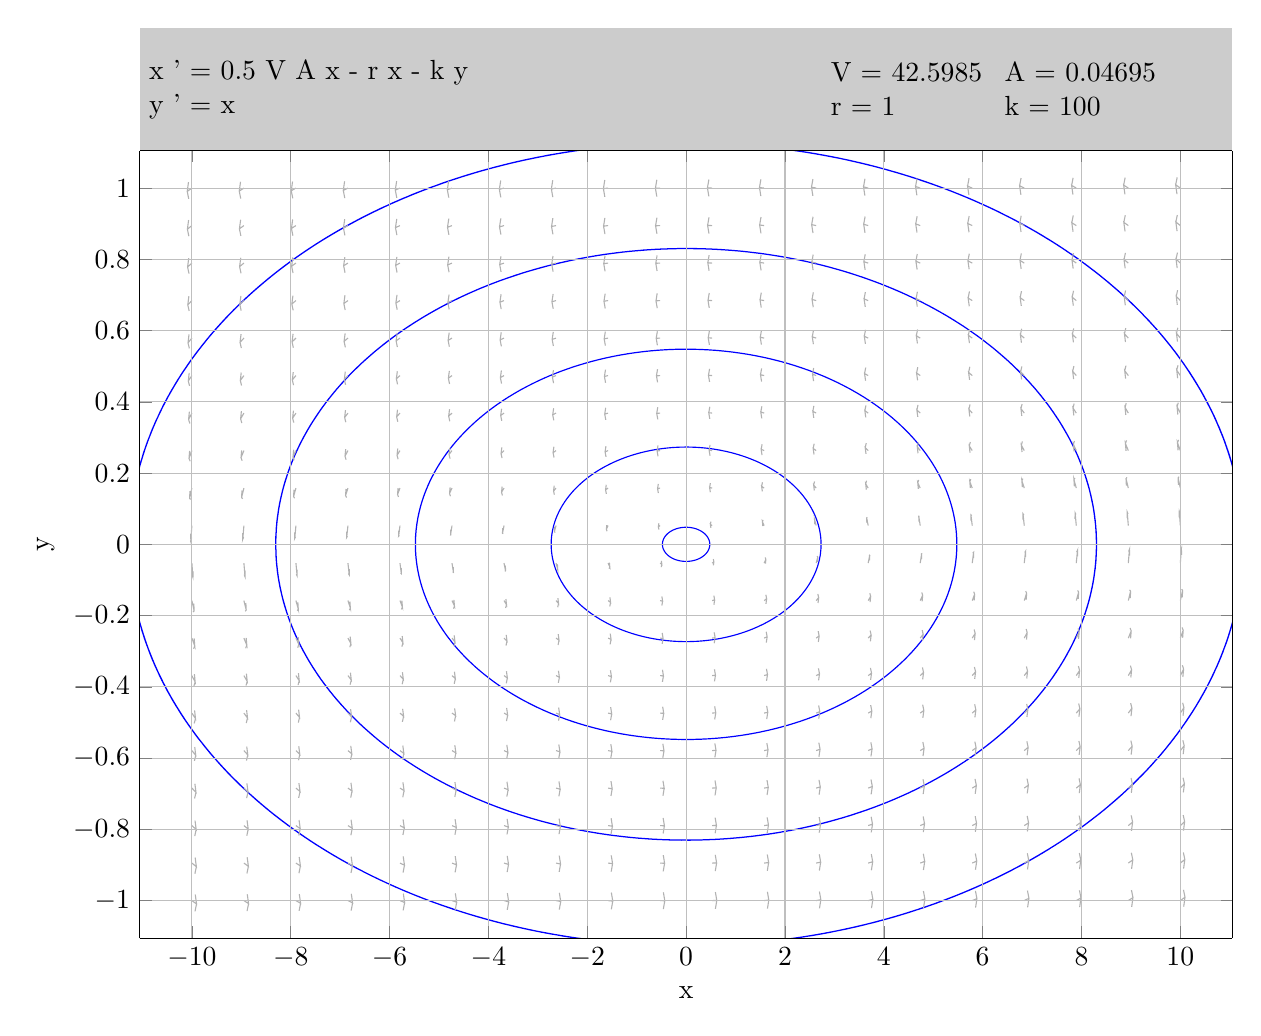
\begin{tikzpicture}

\begin{axis}[%
width=5.4625in,
height=0.614583in,
at={(0.552083in,5.21875in)},
scale only axis,
every outer x axis line/.append style={black},
every x tick label/.append style={font=\color{black}},
xmin=0,
xmax=1,
xtick={-1},
xticklabels={\empty},
every outer y axis line/.append style={black},
every y tick label/.append style={font=\color{black}},
ymin=0,
ymax=1,
ytick={-1},
yticklabels={\empty},
hide axis,
axis background/.style={fill=white!80!black},
axis x line*=bottom,
axis y line*=left
]
\node[right, align=left, inner sep=0mm, text=black]
at (axis cs:0.00806451612903225,0.495614035087719,0) {x ' = 0.5 V A x - r x - k y\\y ' = x};
\node[right, align=left, inner sep=0mm, text=black]
at (axis cs:0.790952380952381,0.5,0) {A = 0.04695\\k = 100};
\node[right, align=left, inner sep=0mm, text=black]
at (axis cs:0.631904761904762,0.5,0) {V = 42.5985\\r = 1};
\node[right, align=left, inner sep=0mm, text=black]
at (axis cs:0.60047619047619,0.5,0) { \\ };
\end{axis}

\begin{axis}[%
width=5.4625in,
height=3.9375in,
at={(0.552083in,1.28125in)},
scale only axis,
unbounded coords=jump,
separate axis lines,
every outer x axis line/.append style={black},
every x tick label/.append style={font=\color{black}},
xmin=-11.0526315789474,
xmax=11.0526315789474,
xlabel={x},
xmajorgrids,
every outer y axis line/.append style={black},
every y tick label/.append style={font=\color{black}},
ymin=-1.10526315789474,
ymax=1.10526315789474,
ylabel={y},
ymajorgrids,
every outer z axis line/.append style={black},
every z tick label/.append style={font=\color{black}},
zmin=-10,
zmax=10,
view={0}{90}
]
\addplot3 [color=blue,solid]
 table[row sep=crcr] {%
0.472349939018912	-0.00819368350852779	-1.64606712607287\\
0.476704534303583	-0.00508191751987662	-1.63951177147786\\
0.479013038376782	-0.0019484171180604	-1.63295641688285\\
0.479263488102984	0.00119340127570465	-1.62640106228784\\
0.477453535357813	0.0043301424340565	-1.61984570769284\\
0.473590447028045	0.00744843232348744	-1.61329035309783\\
0.467691105011605	0.010534918104344	-1.60673499850282\\
0.459782006217568	0.0135762681308271	-1.60017964390781\\
0.449899262566161	0.0165591719509917	-1.5936242893128\\
0.439499787961352	0.0191496113783448	-1.58780082102771\\
0.427611324658005	0.0216751143030523	-1.58197735274263\\
0.414273108845653	0.0241270991509045	-1.57615388445754\\
0.399529497911584	0.0264972766152966	-1.57033041617245\\
0.383429970440839	0.0287776496572288	-1.56450694788737\\
0.366029126216216	0.0309605135053062	-1.55868347960228\\
0.347386686218266	0.0330384556557391	-1.55286001131719\\
0.327567492625294	0.0350043558723429	-1.54703654303211\\
0.309589556044481	0.0366040472380031	-1.54201631420179\\
0.290832023853495	0.0381115154686215	-1.53699608537146\\
0.271341734566481	0.0395229394762747	-1.53197585654114\\
0.251167374959539	0.0408347600404505	-1.52695562771082\\
0.230359480070722	0.0420436798080479	-1.5219353988805\\
0.208970433200039	0.0431466632933775	-1.51691517005018\\
0.187054465909451	0.0441409368781611	-1.51189494121986\\
0.164667658022877	0.0450239888115317	-1.50687471238953\\
0.13842172445238	0.0458989802971013	-1.50110298778057\\
0.111715552542254	0.0466211799395666	-1.4953312631716\\
0.0846375564135622	0.0471880935143708	-1.48955953856263\\
0.0572772045741955	0.0475977852962549	-1.48378781395367\\
0.0297250199188696	0.0478488780592579	-1.4780160893447\\
0.00207257972912569	0.047940553076717	-1.47224436473573\\
-0.0255874843266698	0.0478725501212672	-1.46647264012677\\
-0.0531614861933249	0.0476451674648417	-1.4607009155178\\
-0.0825402730395599	0.0472250641786568	-1.4545094194069\\
-0.111602317998653	0.0466241225254021	-1.44831792329601\\
-0.140236241019647	0.0458444929807917	-1.44212642718511\\
-0.168332839131344	0.0448890534509538	-1.43593493107421\\
-0.195785086442304	0.0437614092724307	-1.42974343496332\\
-0.222488134140846	0.0424658932121784	-1.42355193885242\\
-0.248339310495049	0.0410075654675672	-1.41736044274152\\
-0.273238120852751	0.0393922136663812	-1.41116894663063\\
-0.293698082319945	0.0378913781589071	-1.40587545025272\\
-0.313335282067393	0.0362844569544158	-1.40058195387482\\
-0.332094498037632	0.034575890894571	-1.39528845749691\\
-0.349923233156698	0.0327704113195506	-1.38999496111901\\
-0.366771715334126	0.0308730400680466	-1.38470146474111\\
-0.382592897462944	0.0288890894772651	-1.3794079683632\\
-0.39734245741968	0.0268241623829265	-1.3741144719853\\
-0.41097879806436	0.0246841521192653	-1.36882097560739\\
-0.423439827855202	0.0224796601870146	-1.36353820798309\\
-0.43471969521759	0.0202125056027308	-1.35825544035878\\
-0.44478649288388	0.0178889675139411	-1.35297267273448\\
-0.45361196056898	0.0155154767947014	-1.34768990511017\\
-0.461171484970358	0.0130986160455961	-1.34240713748586\\
-0.467444099768034	0.0106451195937382	-1.33712436986156\\
-0.472412485624584	0.00816187349276921	-1.33184160223725\\
-0.476062970185139	0.00565591552285936	-1.32655883461295\\
-0.478729864701203	0.00255773579406062	-1.32007129836703\\
-0.479384230982005	-0.000551120776297691	-1.31358376212111\\
-0.478021368808912	-0.00365760789106157	-1.3070962258752\\
-0.474645765381737	-0.00674874632461956	-1.30060868962928\\
-0.469271095318737	-0.00981162392290284	-1.29412115338336\\
-0.461920220656617	-0.0128333956033853	-1.28763361713744\\
-0.452625190850524	-0.0158012833550833	-1.28114608089153\\
-0.441427242774052	-0.018702576238556	-1.27465854464561\\
-0.429990293432004	-0.0212004197477259	-1.26892732054133\\
-0.417142321212111	-0.0236286363167564	-1.26319609643706\\
-0.402924542624319	-0.0259792314911632	-1.25746487233279\\
-0.387382842363265	-0.028244505644496	-1.25173364822851\\
-0.370567773308282	-0.0304170539783383	-1.24600242412424\\
-0.352534556523393	-0.0324897665223074	-1.24027120001997\\
-0.333343081257317	-0.0344558281340546	-1.23453997591569\\
-0.313057904943466	-0.0363087184992649	-1.22880875181142\\
-0.294189458345281	-0.03785373338623	-1.22372133612839\\
-0.274560278583885	-0.0393008101384161	-1.21863392044537\\
-0.254220714844778	-0.0406461774698512	-1.21354650476234\\
-0.233222947417716	-0.0418863487494682	-1.20845908907932\\
-0.211620987696708	-0.0430181220011053	-1.2033716733963\\
-0.189470678180014	-0.0440385799035059	-1.19828425771327\\
-0.166829692470149	-0.0449450897903184	-1.19319684203025\\
-0.143757535273881	-0.0457353036500966	-1.18810942634722\\
-0.116011960181092	-0.0465166948221936	-1.1820959597859\\
-0.0878478436332733	-0.0471300161439707	-1.17608249322458\\
-0.0593664448143004	-0.0475729331999768	-1.17006902666326\\
-0.0306699060956308	-0.0478437788846241	-1.16405556010194\\
-0.00186125303630497	-0.047941553402188	-1.15804209354061\\
0.0269556056170536	-0.0478659242668068	-1.15202862697929\\
0.0556758779302388	-0.0476172263024823	-1.14601516041797\\
0.0841938887814614	-0.0471964616430792	-1.14000169385665\\
0.112826494343968	-0.0465951199105541	-1.13389801457975\\
0.14103856295859	-0.0458203736757949	-1.12779433530285\\
0.168724947054608	-0.0448749676746862	-1.12169065602594\\
0.19578297293337	-0.0437623183421144	-1.11558697674904\\
0.222112440768297	-0.0424865138119683	-1.10948329747214\\
0.247615624604878	-0.0410523139171383	-1.10337961819524\\
0.272197272360677	-0.0394651501895173	-1.09727593891834\\
0.295764605825324	-0.0377311258599998	-1.09117225964144\\
0.314795877038187	-0.0361586044498013	-1.08602217706911\\
0.332992424571881	-0.0344902562171311	-1.08087209449677\\
0.350305799851461	-0.0327304533686677	-1.07572201192444\\
0.366690124216132	-0.0308838142920401	-1.07057192935211\\
0.382102088919252	-0.0289552035558272	-1.06542184677977\\
0.396500955128332	-0.026949731909558	-1.06027176420744\\
0.409848553925036	-0.0248727562837118	-1.05512168163511\\
0.422109286305179	-0.0227298797897181	-1.04997159906277\\
0.433554783394769	-0.0204625859383647	-1.04467325146697\\
0.443783785536313	-0.0181379195044008	-1.03937490387116\\
0.452767118845811	-0.0157623599176765	-1.03407655627535\\
0.460479369507979	-0.0133425224967028	-1.02877820867954\\
0.46689888377625	-0.0108851584486517	-1.02347986108374\\
0.472007767972778	-0.00839715486935559	-1.01818151348793\\
0.475791888488431	-0.00588553474330788	-1.01288316589212\\
0.478240871782797	-0.00335745694366268	-1.00758481829631\\
0.479411403391725	-0.000279302937105586	-1.00115843441739\\
0.478604323107374	0.00279992960701023	-0.994732050538466\\
0.475821105011231	0.0058675533953156	-0.988305666659543\\
0.471072018590629	0.00891098597972473	-0.98187928278062\\
0.464376128738744	0.0119177497574354	-0.975452898901697\\
0.455761295754594	0.0148754719709288	-0.969026515022774\\
0.445264175343041	0.0177718847079697	-0.962600131143851\\
0.43293021861479	0.0205948249016063	-0.956173747264928\\
0.420621389832598	0.0230046999841113	-0.950528584112561\\
0.406973392244227	0.0253412774884608	-0.944883420960193\\
0.392028817165996	0.027597091765775	-0.939238257807826\\
0.375834527562556	0.0297649715843156	-0.933593094655458\\
0.358441658046884	0.0318380401294862	-0.92794793150309\\
0.339905614880284	0.0338097150038322	-0.922302768350723\\
0.32028607597239	0.0356737082270406	-0.916657605198355\\
0.299646990881163	0.0374240262359401	-0.911012442045988\\
0.279992771190591	0.0389163929612708	-0.905864375778357\\
0.259597204992882	0.0403056603762333	-0.900716309510726\\
0.238513874952896	0.0415881165316051	-0.895568243243095\\
0.216798169677517	0.0427603554707829	-0.890420176975464\\
0.19450728371565	0.0438192772297829	-0.885272110707834\\
0.171700217558219	0.0447620878372404	-0.880124044440203\\
0.148437777638173	0.04558629931441	-0.874975978172572\\
0.124782576330479	0.0462897296751658	-0.869827911904941\\
0.0957660080853145	0.046976028658747	-0.863607467930576\\
0.0663799266648476	0.0474807348346904	-0.85738702395621\\
0.036737444116733	0.0478017497237409	-0.851166579981845\\
0.00695231059503872	0.0479377463237416	-0.84494613600748\\
-0.0228610856397546	0.0478881691096329	-0.838725692033114\\
-0.0525877182207531	0.0476532340334533	-0.832505248058749\\
-0.0821119226746499	0.0472339285243388	-0.826284804084384\\
-0.111317396421725	0.0466320114885234	-0.820064360110018\\
-0.139191357575383	0.0458773173538997	-0.814040004407172\\
-0.166560047707692	0.0449562956400302	-0.808015648704326\\
-0.193324040439717	0.0438721575550217	-0.801991293001479\\
-0.219386598376192	0.042628736905624	-0.795966937298633\\
-0.244653673105517	0.04123049009723	-0.789942581595787\\
-0.269033905199762	0.0396824961338758	-0.783918225892941\\
-0.292438624214665	0.0379904566182405	-0.777893870190094\\
-0.314781848689635	0.036160695751646	-0.771869514487248\\
-0.33250085265234	0.0345384928280866	-0.766858098127639\\
-0.349385022890032	0.0328296163304557	-0.76184668176803\\
-0.365391785424349	0.031038312823797	-0.75683526540842\\
-0.380480964708293	0.0291690380387108	-0.751823849048811\\
-0.394614783626235	0.0272264568713534	-0.746812432689201\\
-0.407757863493915	0.0252154433834375	-0.741801016329592\\
-0.419877224058441	0.0231410808022321	-0.736789599969983\\
-0.430942283498289	0.0210086615205626	-0.731778183610373\\
-0.441489927919044	0.0186908502258879	-0.726465898206078\\
-0.450792309607006	0.0163203619471665	-0.721153612801783\\
-0.458822691875442	0.0139038411817357	-0.715841327397487\\
-0.465558191832693	0.0114480541569969	-0.710529041993192\\
-0.470979780382169	0.00895988883041543	-0.705216756588897\\
-0.475072282222357	0.00644635488952076	-0.699904471184601\\
-0.477824375846812	0.00391458375190641	-0.694592185780306\\
-0.479228593544164	0.00137182856522996	-0.689279900376011\\
-0.479130823592988	-0.00168324812420888	-0.682906378312832\\
-0.477088952626161	-0.00473142293700676	-0.676532856249652\\
-0.473109490930257	-0.0077603360859304	-0.670159334186473\\
-0.467207402145806	-0.010757762521432	-0.663785812123294\\
-0.459406103267298	-0.0137116119316492	-0.657412290060114\\
-0.449737464643176	-0.0166099287424053	-0.651038767996935\\
-0.438241809975846	-0.019440892117209	-0.644665245933756\\
-0.424967916321665	-0.0221928159572547	-0.638291723870577\\
-0.4119589466804	-0.0245235253759394	-0.632723517547805\\
-0.397673877130106	-0.0267782158162958	-0.627155311225034\\
-0.38215616594356	-0.0289498766789396	-0.621587104902262\\
-0.365453210274918	-0.0310317893754869	-0.61601889857949\\
-0.347616346159712	-0.0330175273285538	-0.610450692256719\\
-0.328700848514852	-0.034900955971757	-0.604882485933947\\
-0.308765931138625	-0.0366762327497133	-0.599314279611176\\
-0.287874746710697	-0.0383378071180399	-0.593746073288404\\
-0.267554181149818	-0.0397826374623464	-0.588544773201569\\
-0.246510514990128	-0.0411198856518314	-0.583343473114734\\
-0.224800194493866	-0.0423459001591746	-0.5781421730279\\
-0.202481443629937	-0.0434573546605766	-0.572940872941065\\
-0.179614264073915	-0.0444512480357585	-0.56773957285423\\
-0.156260435208035	-0.0453249043679619	-0.562538272767395\\
-0.132483514121203	-0.0460759729439492	-0.55733697268056\\
-0.108348835608988	-0.046702428254003	-0.552135672593725\\
-0.0782871535445506	-0.0472994441388549	-0.545741770676213\\
-0.0479064978444605	-0.0477032983131387	-0.5393478687587\\
-0.0173304935115547	-0.0479121660545226	-0.532953966841188\\
0.0133168832854951	-0.0479250893270672	-0.526560064923675\\
0.0439113052121844	-0.0477419767812252	-0.520166163006163\\
0.074328093768175	-0.0473636037538418	-0.513772261088651\\
0.104442219287295	-0.0467916122681545	-0.507378359171138\\
0.13412830093754	-0.046028511033793	-0.500984457253626\\
0.161270162803752	-0.0451492740727197	-0.495032625600591\\
0.187840704004152	-0.0441102634938093	-0.489080793947556\\
0.21374566504038	-0.0429150373460381	-0.483128962294521\\
0.238893616992757	-0.0415677334034159	-0.477177130641486\\
0.263195961520286	-0.0400730691649858	-0.471225298988451\\
0.286566930860654	-0.0384363418548248	-0.465273467335416\\
0.308923587830232	-0.0366634284220434	-0.459321635682381\\
0.330185825824072	-0.0347607855407854	-0.453369804029347\\
0.346876302995457	-0.0330954763463855	-0.44845147363451\\
0.362727908050939	-0.0313501700766373	-0.443533143239673\\
0.377702131837904	-0.0295290482123848	-0.438614812844836\\
0.391762762735166	-0.0276364768477404	-0.433696482449999\\
0.404875886652963	-0.0256770066900847	-0.428778152055162\\
0.417009887032966	-0.0236553730600667	-0.423859821660325\\
0.428135444848271	-0.0215764958916035	-0.418941491265488\\
0.4382255386034	-0.0194454797318808	-0.414023160870651\\
0.448042490837822	-0.0170624619674527	-0.408646723212885\\
0.456565035548633	-0.0146301938532285	-0.403270285555118\\
0.46376799689799	-0.0121556605327773	-0.397893847897351\\
0.469630293450327	-0.00964595946967657	-0.392517410239584\\
0.474134938172356	-0.0071083004475126	-0.387140972581818\\
0.47726903843306	-0.00455000556988006	-0.381764534924051\\
0.4790237960037	-0.00197850926038218	-0.376388097266284\\
0.479394507057814	0.000598641737369253	-0.371011659608517\\
0.478060474970482	0.00362558780983507	-0.364690834468465\\
0.474818601211813	0.00663799441118752	-0.358370009328412\\
0.469680127871408	0.00962384216726163	-0.35204918418836\\
0.462664407958036	0.0125712736949055	-0.345728359048307\\
0.453798905399632	0.0154685936019807	-0.339407533908255\\
0.443119195043299	0.0183042684873617	-0.333086708768202\\
0.430668962655309	0.0210669269409364	-0.32676588362815\\
0.416500004921101	0.023745359543606	-0.320445058488097\\
0.402846300841745	0.0259946022643773	-0.314956142942352\\
0.387979984727945	0.0281655459836513	-0.309467227396606\\
0.371945080490393	0.0302516299303607	-0.303978311850861\\
0.354789229537339	0.0322465811175034	-0.298489396305115\\
0.336563690774594	0.0341444143421425	-0.29300048075937\\
0.317323340605524	0.0359394321854064	-0.287511565213624\\
0.297126672931056	0.037626225012489	-0.282022649667879\\
0.276035799149674	0.0391996709726492	-0.276533734122134\\
0.255067060427958	0.0405953758196265	-0.271279188862428\\
0.233394823094486	0.0418790446866911	-0.266024643602723\\
0.211078427986046	0.0430470955401461	-0.260770098343017\\
0.188178958741213	0.0440962912493767	-0.255515553083312\\
0.164759241800344	0.0450237395868505	-0.250261007823606\\
0.140883846405581	0.0458268932281166	-0.245006462563901\\
0.11661908460085	0.0465035497518067	-0.239751917304196\\
0.0920330112318597	0.0470518516396343	-0.23449737204449\\
0.0609984334877816	0.0475540364026384	-0.227938812659807\\
0.0297025659000805	0.0478519108237702	-0.221380253275123\\
-0.00172050790097811	0.0479439898198387	-0.21482169389044\\
-0.0331367116323003	0.0478297520544313	-0.208263134505757\\
-0.0644119763579648	0.0475096399379138	-0.201704575121073\\
-0.0954122404892226	0.04698505962743	-0.19514601573639\\
-0.126003449784497	0.0462583810269022	-0.188587456351707\\
-0.156051557349384	0.0453329377870309	-0.182028896967023\\
-0.182347502594057	0.0443407146531739	-0.176165796268811\\
-0.208016638816696	0.0431962189237738	-0.170302695570599\\
-0.232970566005536	0.0419032724871922	-0.164439594872387\\
-0.257123785590469	0.0404662297180068	-0.158576494174175\\
-0.280393700443037	0.0388899774770116	-0.152713393475963\\
-0.302700614876441	0.0371799351112169	-0.146850292777751\\
-0.323967734645533	0.0353420544538491	-0.140987192079539\\
-0.34412116694682	0.0333828198243506	-0.135124091381327\\
-0.360346358152047	0.0316245946591019	-0.130133382158054\\
-0.375674296171212	0.0297876656312202	-0.12514267293478\\
-0.390066601814746	0.0278765653315502	-0.120151963711507\\
-0.403487417574662	0.0258960115968864	-0.115161254488234\\
-0.415903407624546	0.0238509075099737	-0.110170545264961\\
-0.427283757819565	0.021746341399507	-0.105179836041688\\
-0.437600175696461	0.0195875868401316	-0.100189126818415\\
-0.446826890473555	0.0173801026524428	-0.0951984175951415\\
-0.455946443251593	0.0148238457420397	-0.089536710633844\\
-0.463605442247055	0.0122201546960273	-0.0838750036725466\\
-0.469778562285425	0.00957732274626625	-0.0782132967112491\\
-0.474445612850315	0.00690375306186097	-0.0725515897499517\\
-0.477591538083464	0.00420795874915941	-0.0668898827886542\\
-0.479206416784739	0.00149856285175309	-0.0612281758273568\\
-0.479285462412135	-0.0012157016495229	-0.0555664688660594\\
-0.477829023081771	-0.00392599183658988	-0.0499047619047619\\
-0.474453481613825	-0.00689716370298624	-0.0436666666666667\\
-0.469233696959843	-0.00984145732084112	-0.0374285714285714\\
-0.462188385348514	-0.0127474215512782	-0.0311904761904762\\
-0.453343825406282	-0.0156038092188807	-0.024952380952381\\
-0.442733858157346	-0.0183995771116909	-0.0187142857142857\\
-0.430399887023659	-0.0211238859812108	-0.0124761904761905\\
-0.416390877824931	-0.0237661005424016	-0.00623809523809524\\
-0.400763358778626	-0.0263157894736841	0\\
-0.400763358778626	-0.0263157894736841	0\\
-0.383577962778391	-0.0287631817180492	0.00623809523809524\\
-0.364900252833042	-0.0310988299503879	0.0124761904761905\\
-0.344803482100006	-0.0333134010783585	0.0187142857142857\\
-0.323365781028566	-0.0353981748880104	0.024952380952381\\
-0.300670157359863	-0.0373450440437843	0.0311904761904762\\
-0.276804496126894	-0.0391465140885122	0.0374285714285714\\
-0.251861559654514	-0.0407957034434172	0.0436666666666667\\
-0.225938987559431	-0.0422863434081135	0.0499047619047619\\
-0.198970028693154	-0.0436203662307742	0.0561810424577956\\
-0.171216686445902	-0.0447827446372258	0.0624573230108293\\
-0.142790003357038	-0.0457687065716205	0.068733603563863\\
-0.113802393103769	-0.0465742714648751	0.0750098841168967\\
-0.0843676405011445	-0.0471962502346717	0.0812861646699304\\
-0.0546009015020553	-0.0476322452854571	0.0875624452229641\\
-0.0246187031972348	-0.0478806505084431	0.0938387257759978\\
0.00546105618474169	-0.0479406512816064	0.100115006329032\\
0.0308521592957995	-0.0478444209897781	0.105415267233242\\
0.0561572039448811	-0.0476138391772894	0.110715528137452\\
0.0813040345199254	-0.0472495222998991	0.116015789041663\\
0.106221633434798	-0.0467524707187527	0.121316049945873\\
0.130840121129293	-0.0461240687003823	0.126616310850084\\
0.155090756069127	-0.0453660844167065	0.131916571754294\\
0.178905934745948	-0.0444806699450304	0.137216832658504\\
0.202219191677328	-0.0434703612680458	0.142517093562715\\
0.223463467360621	-0.0424174613421305	0.147462919546535\\
0.24416168824809	-0.0412608222065719	0.152408745530355\\
0.264262447053602	-0.0400032855873258	0.157354571514175\\
0.283716269703558	-0.0386479246244133	0.162300397497995\\
0.302475615336899	-0.0371980438719208	0.167246223481815\\
0.320494876305102	-0.0356571792980003	0.172192049465635\\
0.337730378172181	-0.034029098284869	0.177137875449455\\
0.35414037971469	-0.0323177996288097	0.182083701433275\\
0.372845304508079	-0.0301407375355802	0.188070986385622\\
0.390215193421375	-0.027855617069315	0.194058271337969\\
0.406185981099292	-0.0254707267830049	0.200045556290316\\
0.420699604284639	-0.0229946324727201	0.206032841242663\\
0.433704001818317	-0.0204361771776097	0.21202012619501\\
0.445153114639326	-0.0178044811799019	0.218007411147358\\
0.455006885784759	-0.0151089420049039	0.223994696099705\\
0.463231260389805	-0.012359234421002	0.229981981052052\\
0.470107863538638	-0.00941153056058939	0.236295975693653\\
0.475112009921908	-0.00642620227527916	0.242609970335254\\
0.478222209599846	-0.0034153683793843	0.248923964976856\\
0.479425192028837	-0.000391098298140449	0.255237959618457\\
0.478715906061423	0.00263458793229412	0.261551954260059\\
0.476097519946295	0.00564971966483851	0.26786594890166\\
0.471581421328299	0.00864237564148915	0.274179943543261\\
0.465187217248436	0.0116006839933199	0.280493938184863\\
0.458561780651343	0.0139921687514454	0.285670388494389\\
0.450707963810138	0.0163462253833195	0.290846838803916\\
0.441646766701927	0.0186564473486808	0.296023289113443\\
0.431402351119138	0.0209166072797374	0.301199739422969\\
0.420002040669527	0.0231206569811662	0.306376189732496\\
0.407476320776169	0.0252627274301137	0.311552640042023\\
0.393858838677466	0.0273371287761953	0.31672909035155\\
0.379186403427143	0.0293383503414957	0.321905540661076\\
0.362156929883549	0.0314163924523825	0.327509920028267\\
0.343990062969367	0.033395868146566	0.333114299395458\\
0.324743358583919	0.0352704217941057	0.338718678762649\\
0.304477306327283	0.0370341070460157	0.34432305812984\\
0.283255329500288	0.0386813868342641	0.349927437497031\\
0.261143785104519	0.0402071333717737	0.355531816864222\\
0.238211963842314	0.0416066281524213	0.361136196231413\\
0.214532090116763	0.0428755619510384	0.366740575598604\\
0.186677776765631	0.0441596763067818	0.373138734088051\\
0.158058552322382	0.0452632171056612	0.379536892577499\\
0.128793505574685	0.0461814578760148	0.385935051066947\\
0.0990029365816018	0.0469105334661095	0.392333209556394\\
0.0688083566735957	0.0474474400441404	0.398731368045842\\
0.0383324884525253	0.0477900350982315	0.40512952653529\\
0.00769926579164687	0.0479370374364349	0.411527685024737\\
-0.0229661661643868	0.0478880271867313	0.417925843514185\\
-0.0483309123018248	0.0476988652199288	0.423231574515453\\
-0.0735602404623238	0.0473754819055559	0.42853730551672\\
-0.0985820451864961	0.046918760022295	0.433843036517988\\
-0.123325504835967	0.0463299634141977	0.439148767519256\\
-0.147721081593374	0.0456107369906845	0.444454498520523\\
-0.171700521462369	0.0447631067265449	0.449760229521791\\
-0.195196854267614	0.0437894796619373	0.455065960523059\\
-0.218144393654787	0.0426926439023892	0.460371691524326\\
-0.239533852451803	0.041530340555181	0.465449674105982\\
-0.260306300658896	0.0402609665661296	0.470527656687639\\
-0.280407292879032	0.0388878119298766	0.475605639269295\\
-0.299784646321471	0.0374144149204995	0.480683621850951\\
-0.318388440801772	0.0358445620915117	0.485761604432607\\
-0.336171018741787	0.0341822882758626	0.490839587014264\\
-0.353086985169663	0.0324318765859372	0.49591756959592\\
-0.369093207719846	0.0305978584135565	0.500995552177576\\
-0.386953167969806	0.028305579492546	0.507057320201926\\
-0.40339288143045	0.0259092722078788	0.513119088226276\\
-0.418350073649968	0.0234178530844273	0.519180856250626\\
-0.431768926156415	0.0208404980084098	0.525242624274975\\
-0.44360007645771	0.0181866422273903	0.531304392299325\\
-0.453800618041636	0.0154659803502783	0.537366160323675\\
-0.46233410037584	0.012688466347329	0.543427928348025\\
-0.469170528907834	0.00986431355014311	0.549489696372375\\
-0.474329046989909	0.00697430741125383	0.555613590104108\\
-0.477710140278669	0.00405804901501974	0.56173748383584\\
-0.47929993008002	0.00112666966017347	0.567861377567573\\
-0.479091753964478	-0.00180877581940653	0.573985271299306\\
-0.477086165767175	-0.00473730905469607	0.580109165031039\\
-0.473290935587858	-0.00764802814152519	0.586233058762771\\
-0.467721049790886	-0.0105301076405781	0.592356952494504\\
-0.460398711005235	-0.0133727985773934	0.598480846226237\\
-0.452952431920263	-0.0157112942968085	0.603600254815057\\
-0.444319361967784	-0.0180086759263159	0.608719663403878\\
-0.43452212342506	-0.0202588289321279	0.613839071992699\\
-0.423586296961713	-0.0224558206646071	0.618958480581519\\
-0.411540421639724	-0.0245939003582668	0.62407788917034\\
-0.398415994913438	-0.0266674991317702	0.62919729775916\\
-0.384247472629561	-0.0286712299879314	0.634316706347981\\
-0.369072269027159	-0.0305998878137145	0.639436114936802\\
-0.351085445767778	-0.0326479868144293	0.64512216477188\\
-0.331963598678318	-0.0345906490852052	0.650808214606959\\
-0.311769126358319	-0.0364214467419406	0.656494264442037\\
-0.29056737676909	-0.0381343975933997	0.662180314277116\\
-0.268426647233713	-0.0397239651412122	0.667866364112194\\
-0.245418184437043	-0.0411850585798738	0.673552413947273\\
-0.221616184425703	-0.0425130327967458	0.679238463782351\\
-0.19709779260809	-0.0437036883720552	0.68492451361743\\
-0.168493658964877	-0.0448842519980213	0.691379684772132\\
-0.13918659143366	-0.0458779927554216	0.697834855926833\\
-0.109300808923042	-0.0466805589747847	0.704290027081535\\
-0.0789614052510606	-0.0472884970596774	0.710745198236237\\
-0.0482943491451907	-0.0476992514867039	0.717200369390938\\
-0.0174264842423397	-0.0479111648055068	0.72365554054564\\
0.01351447091115	-0.047923477638766	0.730110711700342\\
0.0443999228595019	-0.0477363286821997	0.736565882855043\\
0.069583905361701	-0.0474347370457778	0.741856825167833\\
0.0945737462902828	-0.0470004073429462	0.747147767480623\\
0.119298409683341	-0.0464345331550471	0.752438709793412\\
0.143688293806055	-0.0457386788145119	0.757729652106202\\
0.167675231150683	-0.0449147794048613	0.763020594418992\\
0.191192488436572	-0.0439651407607052	0.768311536731781\\
0.214174766610149	-0.0428924394677427	0.773602479044571\\
0.236558200844925	-0.0416997228627621	0.77889342135736\\
0.257992516961881	-0.0404087362730329	0.78411301235971\\
0.278724707125643	-0.0390076781250497	0.789332603362059\\
0.298697284205325	-0.0375003883298879	0.794552194364408\\
0.317855429683961	-0.0358909716642972	0.799771785366758\\
0.336146993658501	-0.0341837977707011	0.804991376369107\\
0.353522494839814	-0.0323835011571972	0.810210967371457\\
0.369935120552685	-0.0304949811975571	0.815430558373806\\
0.385340726735821	-0.0285234021312263	0.820650149376156\\
0.402132858764207	-0.0261028330131149	0.8267956374488\\
0.417407968976286	-0.0235836511324559	0.832941125521444\\
0.431106431036867	-0.0209754997204426	0.839086613594088\\
0.443175599554074	-0.0182882560627445	0.845232101666732\\
0.453569810079346	-0.0155320314995075	0.851377589739377\\
0.46225037910744	-0.0127171714253538	0.857523077812021\\
0.469185604076427	-0.00985425528938206	0.863668565884665\\
0.474350763367695	-0.00695409659516706	0.869814053957309\\
0.477626779538944	-0.00414463827657962	0.875714417327927\\
0.479241088102068	-0.00132066272235495	0.881614780698544\\
0.479187196667145	0.00150782989044877	0.887515144069162\\
0.477464759874268	0.004330937142441	0.893415507439779\\
0.474079579393552	0.00713885437189876	0.899315870810397\\
0.469043603925127	0.00992187467476675	0.905216234181014\\
0.462374929199142	0.0126703889046572	0.911116597551632\\
0.454097797975766	0.0153748856728501	0.917016960922249\\
0.445748130851776	0.017650026348659	0.922072458872568\\
0.436259495459907	0.0198801170997161	0.927127956822887\\
0.425656181205626	0.0220593705380582	0.932183454773205\\
0.413965214561674	0.0241821833635341	0.937238952723524\\
0.401216359068072	0.0262431363638045	0.942294450673843\\
0.387442115332119	0.0282369944143419	0.947349948624162\\
0.372677721028391	0.0301587064784306	0.952405446574481\\
0.356961150898742	0.032003405607167	0.957460944524799\\
0.337891866162452	0.034010679455947	0.963236516623304\\
0.317695501054446	0.0359046308276662	0.969012088721808\\
0.296440100036819	0.0376787852400384	0.974787660820313\\
0.274196647664562	0.0393271564634472	0.980563232918817\\
0.251039068585561	0.0408442465209453	0.986338805017322\\
0.227044227540598	0.0422250456882554	0.992114377115826\\
0.202291929363349	0.0434650324937695	0.997889949214331\\
0.176864918980387	0.0445601737185494	1.00366552131284\\
0.147455201657991	0.0456179868549512	1.01018538188614\\
0.117417700184293	0.0464820971932555	1.01670524245944\\
0.0868823965776233	0.0471486194012056	1.02322510303275\\
0.0559797301141182	0.0476146073970944	1.02974496360605\\
0.0248405973277185	0.0478780543497648	1.03626482417935\\
-0.0064036479898299	0.0479378926786095	1.04278468475266\\
-0.0376211947889752	0.0477939940535709	1.04930454532596\\
-0.0686797747623613	0.0474471693951416	1.05582440589926\\
-0.0936007011320971	0.0470190908382147	1.06109915185892\\
-0.118261869875659	0.0464602382934155	1.06637389781858\\
-0.142593593585855	0.0457721502550669	1.07164864377824\\
-0.166527783326108	0.0449567237490439	1.07692338973789\\
-0.18999794863045	0.0440162143327738	1.08219813569755\\
-0.212939197503527	0.0429532360952362	1.08747288165721\\
-0.235288236420595	0.0417707616569629	1.09274762761687\\
-0.256983370327525	0.0404721221700382	1.09802237357652\\
-0.278311107025898	0.0390362599116746	1.10338575579512\\
-0.298839127244176	0.0374881232849145	1.10874913801373\\
-0.318507242178641	0.0358321965507157	1.11411252023233\\
-0.337258408054197	0.0340732428435476	1.11947590245093\\
-0.355038726124373	0.0322163041713916	1.12483928466953\\
-0.371797442671316	0.0302667014157409	1.13020266688813\\
-0.387486949005796	0.0282300343316007	1.13556604910673\\
-0.402062781467208	0.0261121815474876	1.14092943132533\\
-0.417557115532075	0.0235554463399169	1.14716594827353\\
-0.431429218962429	0.0209070507573579	1.15340246522173\\
-0.443623133942385	0.0181774457932428	1.15963898216993\\
-0.454090466784568	0.0153772824220498	1.16587549911813\\
-0.462790387930112	0.0125174115993027	1.17211201606633\\
-0.469689631948665	0.00960888426157127	1.17834853301453\\
-0.474762497538385	0.00666295132647094	1.18458504996273\\
-0.477990847525939	0.00369106369266295	1.19082156691093\\
-0.479311993671851	0.000990346126314353	1.19646218113378\\
-0.4791089768626	-0.0017135987580468	1.20210279535664\\
-0.477381861252115	-0.00441202785952765	1.20774340957949\\
-0.474135762773675	-0.00709630834695328	1.21338402380234\\
-0.469380849139917	-0.00975791765886669	1.2190246380252\\
-0.463132339842833	-0.0123884435035288	1.22466525224805\\
-0.455410506153773	-0.0149795838589184	1.2303058664709\\
-0.446240671123438	-0.0175231469727324	1.23594648069376\\
-0.436953845201617	-0.019725197664544	1.24093185617986\\
-0.426581247996145	-0.0218782807010503	1.24591723166597\\
-0.415148737496948	-0.0239769633123169	1.25090260715207\\
-0.402684676727771	-0.026015997902132	1.25588798263818\\
-0.38921993374617	-0.0279903220480065	1.26087335812428\\
-0.374787881643521	-0.0298950585011741	1.26585873361039\\
-0.359424398545011	-0.0317255151865911	1.2708441090965\\
-0.343167867609647	-0.0334771852029367	1.2758294845826\\
-0.322938805597437	-0.0354326741545225	1.2816987844119\\
-0.301597240537955	-0.0372662406237584	1.28756808424119\\
-0.279217484555615	-0.0389714011075097	1.29343738407049\\
-0.255876747323886	-0.040542207775713	1.29930668389979\\
-0.231655136065287	-0.0419732484713764	1.30517598372908\\
-0.206635655551393	-0.0432596467105794	1.31104528355838\\
-0.18090420810283	-0.0443970616824728	1.31691458338767\\
-0.154549593589277	-0.0453816882492791	1.32278388321697\\
-0.124525151251781	-0.0462957722731354	1.32933112946908\\
-0.0939658146452914	-0.047011614995296	1.33587837572119\\
-0.0630050273680229	-0.0475259427511925	1.3424256219733\\
-0.031776213185733	-0.0478364386994103	1.34897286822541\\
-0.000412776031722378	-0.0479417428216893	1.35552011447752\\
0.0309518999931657	-0.0478414519229234	1.36206736072964\\
0.0621844506205445	-0.0475361196311606	1.36861460698175\\
0.0931515314144857	-0.0470272563976033	1.37516185323386\\
0.117705833132736	-0.0464735519679776	1.38041267442202\\
0.141936281804149	-0.0457917572345146	1.38566349561019\\
0.165775015643331	-0.0449837415484133	1.39091431679836\\
0.189155918141239	-0.0440517177577544	1.39616513798652\\
0.212014618065188	-0.0429982422075003	1.40141595917469\\
0.234288489458846	-0.0418262147394949	1.40666678036285\\
0.255916651642236	-0.0405388786924641	1.41191760155102\\
0.276839969211735	-0.0391398209020153	1.41716842273919\\
0.29791770218603	-0.0375603952111103	1.42266290282249\\
0.318097030158014	-0.0358675912939475	1.42815738290578\\
0.337315765015468	-0.0340665598822507	1.43365186298908\\
0.355515357793947	-0.0321627398273175	1.43914634307238\\
0.372640898676778	-0.0301618581000189	1.44464082315568\\
0.388641116995064	-0.0280699297907996	1.45013530323898\\
0.403468381227682	-0.0258932581096778	1.45562978332227\\
0.417078699001283	-0.0236384343862453	1.46112426340557\\
0.431186580627018	-0.020954991306573	1.46744872466277\\
0.44357169024004	-0.0181876726052399	1.47377318591996\\
0.454182432605992	-0.0153477200076467	1.48009764717716\\
0.46297534663258	-0.0124465354231667	1.48642210843435\\
0.469915105369573	-0.00949568094514548	1.49274656969155\\
0.474974516008804	-0.00650687885090141	1.49907103094874\\
0.478134519884166	-0.00349201160172526	1.50539549220594\\
0.479384192471618	-0.000463121842880294	1.51171995346313\\
};
 \addplot3 [color=blue,solid]
 table[row sep=crcr] {%
2.72005328811045	-0.024521287035537	-2.13113665303697\\
2.73019706801791	-0.00699456547216167	-2.12470727888917\\
2.72906801076866	0.0105606162833134	-2.11827790474138\\
2.71666020036389	0.0280718792592372	-2.11184853059358\\
2.69301803003992	0.0454673438928913	-2.10541915644578\\
2.65823620226815	0.0626756300304909	-2.09898978229798\\
2.6124597287551	0.0796258569271838	-2.09256040815019\\
2.55588393044238	0.096247643247051	-2.08613103400239\\
2.4887544375067	0.112471107063107	-2.07970165985459\\
2.42116368732469	0.126367074145266	-2.07404283892985\\
2.34582711213771	0.139858449987052	-2.06838401800511\\
2.26298073188629	0.152901928600625	-2.06272519708036\\
2.17288546264886	0.165455850740362	-2.05706637615562\\
2.07582711664181	0.177480203902856	-2.05140755523087\\
1.97211640221946	0.188936622326917	-2.04574873430613\\
1.86208892387406	0.19978838699357	-2.04008991338139\\
1.7461051822358	0.210000425626058	-2.03443109245664\\
1.63852012853931	0.218498623241327	-2.0294105685278\\
1.52680869802916	0.226446267085863	-2.02439004459896\\
1.41125006213623	0.233823185682632	-2.01936952067013\\
1.29213303192739	0.240610758855701	-2.01434899674129\\
1.16975605810554	0.246791917730241	-2.00932847281245\\
1.04442723100958	0.25235114473252	-2.00430794888361\\
0.916464280614432	0.257274473589911	-1.99928742495477\\
0.786194576531029	0.261549489330884	-1.99426690102593\\
0.627980979980193	0.265792935946757	-1.98826818335465\\
0.467513037631457	0.269080746598261	-1.98226946568337\\
0.305364950948032	0.271400432042978	-1.97627074801209\\
0.142115450170806	0.272743271910281	-1.97027203034081\\
-0.0216522056816528	0.273104314701338	-1.96427331266952\\
-0.185350228813103	0.272482377789107	-1.95827459499824\\
-0.348386302649623	0.27088004741834	-1.95227587732696\\
-0.510163581839617	0.268303678705581	-1.94627715965568\\
-0.671806384198582	0.264719940639976	-1.94021389768614\\
-0.830978364013939	0.260164030370535	-1.93415063571659\\
-0.987094083977168	0.254651919411996	-1.92808737374705\\
-1.13958218430043	0.248203288553374	-1.92202411177751\\
-1.28788538271659	0.24084152785797	-1.91596084980796\\
-1.43146047447916	0.232593736663365	-1.90989758783842\\
-1.56977833236238	0.223490723581425	-1.90383432586888\\
-1.70232390666114	0.213567006498297	-1.89777106389934\\
-1.80873560083424	0.204633371044129	-1.89268317147875\\
-1.91046627659829	0.195170426393202	-1.88759527905816\\
-2.00725161124644	0.185202386851035	-1.88250738663757\\
-2.09884129120844	0.174754792649021	-1.87741949421698\\
-2.18499901205058	0.163854509944439	-1.87233160179639\\
-2.26550247847573	0.152529730820441	-1.8672437093758\\
-2.34014340432334	0.140809973286065	-1.86215581695522\\
-2.40872751256943	0.128726081276224	-1.85706792453463\\
-2.47264939917496	0.115975363665583	-1.85184479632513\\
-2.52982881058753	0.102908631375915	-1.84662166811562\\
-2.58010736705906	0.0895612840389206	-1.84139853990612\\
-2.62334689278108	0.0759694501903525	-1.83617541169662\\
-2.65942941588469	0.0621699872700111	-1.83095228348712\\
-2.68825716844054	0.0482004816217467	-1.82572915527762\\
-2.70975258645889	0.0340992484934588	-1.82050602706811\\
-2.72385830988955	0.0199053320370964	-1.81528289885861\\
-2.73102316432622	0.0024228957261104	-1.80887520496654\\
-2.72698762313386	-0.0150690612675198	-1.80246751107447\\
-2.71175784489234	-0.0324988910682224	-1.79605981718239\\
-2.68538951365602	-0.0497955181577154	-1.78965212329032\\
-2.64798783895383	-0.0668884393750076	-1.78324442939825\\
-2.59970755578924	-0.0837077239163978	-1.77683673550618\\
-2.54075292464028	-0.100184013335475	-1.7704290416141\\
-2.47137773145949	-0.11624852154312	-1.76402134772203\\
-2.40208410998038	-0.129965174369153	-1.75839374805138\\
-2.3251902013905	-0.143270300340277	-1.75276614838073\\
-2.24093446819922	-0.156121657109124	-1.74713854871008\\
-2.1495794796752	-0.168478646181987	-1.74151094903943\\
-2.05141191184638	-0.180302312918822	-1.73588334936878\\
-1.94674254749993	-0.191555346533246	-1.73025574969813\\
-1.83590627618234	-0.20220208009254	-1.72462815002748\\
-1.71926209419934	-0.212208490517649	-1.71900055035683\\
-1.61011506167201	-0.220604808483733	-1.7139579158822\\
-1.49687747364557	-0.228440364919122	-1.70891528140757\\
-1.37983483471164	-0.235695088979216	-1.70387264693294\\
-1.25928225054607	-0.242350502390465	-1.69883001245831\\
-1.13552442790896	-0.248389719450377	-1.69378737798368\\
-1.00887567464463	-0.253797447027513	-1.68874474350905\\
-0.87965989968167	-0.258559984561489	-1.68370210903442\\
-0.748210613032879	-0.262665224062976	-1.67865947455979\\
-0.587406166448224	-0.266722902674204	-1.67258613060176\\
-0.424440601455662	-0.269797633860662	-1.66651278664374\\
-0.259911761362613	-0.27187736229191	-1.66043944268571\\
-0.0944215688448314	-0.272954006534064	-1.65436609872768\\
0.0714239740535992	-0.273023459049792	-1.64829275476965\\
0.237014785920267	-0.272085586198318	-1.64221941081163\\
0.401736705974428	-0.270144228235422	-1.6361460668536\\
0.564971494067011	-0.267207199313435	-1.63007272289557\\
0.725104162196063	-0.263313877051858	-1.62403775872974\\
0.882595088216693	-0.258462544741317	-1.6180027945639\\
1.03687029807255	-0.252670114109357	-1.61196783039807\\
1.1873703295129	-0.245957107790862	-1.60593286623224\\
1.33355023209263	-0.238347659328051	-1.5998979020664\\
1.47487956717224	-0.229869513170483	-1.59386293790057\\
1.61084240791785	-0.220554024675048	-1.58782797373473\\
1.74093733930122	-0.210436160105978	-1.5817930095689\\
1.8447081831188	-0.201401698010562	-1.57675471105904\\
1.94379752596318	-0.191856385709951	-1.57171641254917\\
2.03795288713047	-0.181824186722577	-1.56667811403931\\
2.12693545289721	-0.17133031596299	-1.56163981552944\\
2.21052007652037	-0.160401239741861	-1.55660151701958\\
2.28849527823732	-0.149064675765977	-1.55156321850971\\
2.36066324526591	-0.137349593138245	-1.54652491999985\\
2.42683983180435	-0.125286212357692	-1.54148662148998\\
2.48898979851381	-0.112434863092836	-1.53625916996468\\
2.54434153445495	-0.0992766468387725	-1.53103171843938\\
2.59274134781872	-0.0858472747829584	-1.52580426691408\\
2.63405592278643	-0.0721831602701666	-1.52057681538878\\
2.66817231952966	-0.0583214188024845	-1.51534936386348\\
2.69499797421037	-0.0442998680393139	-1.51012191233818\\
2.7144606989808	-0.0301570277973715	-1.50489446081288\\
2.72650868198353	-0.0159321200506883	-1.49966700928757\\
2.73112666169772	0.0015081559148747	-1.49327798514125\\
2.72460893904264	0.0189418699374651	-1.48688896099492\\
2.7069718565124	0.0362980155399247	-1.48049993684859\\
2.67828060511292	0.0535062194729434	-1.47411091270226\\
2.63864922436194	0.0704967417150605	-1.46772188855593\\
2.58824060228901	0.0872004754726638	-1.4613328644096\\
2.52726647543549	0.10354894717999	-1.45494384026327\\
2.45598742885454	0.119474316499126	-1.44855481611695\\
2.38526552946657	0.133034437740652	-1.44295441083702\\
2.3070692649792	0.146177379201354	-1.43735400555709\\
2.22163897520735	0.158861812334306	-1.43175360027716\\
2.12923843456594	0.171048048535108	-1.42615319499723\\
2.03015485206986	0.18269803914188	-1.4205527897173\\
1.92469887133396	0.19377537543527	-1.41495238443737\\
1.81320457057307	0.204245288638451	-1.40935197915744\\
1.696029462602	0.214074649917117	-1.40375157387751\\
1.58554817475855	0.222381675012543	-1.39868990899436\\
1.47100835456747	0.23011915256912	-1.39362824411121\\
1.35270099240645	0.237267105690901	-1.38856657922806\\
1.23092664158517	0.243807185993522	-1.38350491434492\\
1.10599541834526	0.249722673604203	-1.37844324946177\\
0.978227001860298	0.25499847716175	-1.37338158457862\\
0.847950634235811	0.259621133816551	-1.36831991969547\\
0.715505120509289	0.263578809230579	-1.36325825481232\\
0.552513056201554	0.26747137248805	-1.35712159500129\\
0.387445972353519	0.270357606866634	-1.35098493519026\\
0.2209222160521	0.272225879113697	-1.34484827537923\\
0.0535637770064339	0.273068709690298	-1.3387116155682\\
-0.114003712452129	0.272882772771184	-1.33257495575717\\
-0.281150977370024	0.271668896244789	-1.32643829594614\\
-0.447245100171471	0.269432061713242	-1.32030163613511\\
-0.611649520658474	0.266181404492356	-1.31416497632408\\
-0.770439797668778	0.262027196775526	-1.30815439211485\\
-0.926446002997973	0.25692734157651	-1.30214380790561\\
-1.07910406367749	0.250899523202168	-1.29613322369638\\
-1.22786476532226	0.243964952934049	-1.29012263948714\\
-1.37219375213067	0.236148369028394	-1.28411205527791\\
-1.51157152688461	0.227478036716132	-1.27810147106867\\
-1.64549345094944	0.217985748202884	-1.27209088685944\\
-1.77346974427401	0.207706822668958	-1.26608030265021\\
-1.8749571099155	0.198593924881246	-1.26108570191144\\
-1.97176838399181	0.188985993097327	-1.25609110117267\\
-2.06366113927199	0.178906741468052	-1.2510965004339\\
-2.15040630546246	0.168381073033381	-1.24610189969513\\
-2.23178816920709	0.157435079722387	-1.24110729895636\\
-2.30760437408716	0.146096042353253	-1.23611269821759\\
-2.37766592062135	0.134392430633274	-1.23111809747882\\
-2.44179716626576	0.122353903158856	-1.22612349674005\\
-2.50243500204054	0.109419160862517	-1.22089235137794\\
-2.55622825666567	0.0961853668770634	-1.21566120601583\\
-2.60302724859367	0.0826884922397613	-1.21043006065372\\
-2.64270281591808	0.0689651872498521	-1.20519891529161\\
-2.67514631637351	0.0550527814685509	-1.19996776992951\\
-2.70026962733564	0.0409892837190466	-1.1947366245674\\
-2.71800514582116	0.0268133820865021	-1.18950547920529\\
-2.72830578848783	0.0125644439180545	-1.18427433384318\\
-2.73077753668196	-0.00483718929668016	-1.17790114968994\\
-2.72217009855245	-0.0222187873649526	-1.1715279655367\\
-2.70250829816232	-0.0395098961589217	-1.16515478138346\\
-2.67186523257963	-0.0566407449999592	-1.15878159723023\\
-2.63036227187754	-0.0735422466586499	-1.15240841307699\\
-2.57816905913427	-0.0901459973547919	-1.14603522892375\\
-2.51550351043311	-0.106384276757396	-1.13966204477051\\
-2.44263181486245	-0.122190047984688	-1.13328886061727\\
-2.37072634772486	-0.135615977989002	-1.12771173085942\\
-2.29145364820646	-0.14862016380636	-1.12213460110158\\
-2.20505548754418	-0.161162049616122	-1.11655747134374\\
-2.11179650750607	-0.173202715232799	-1.11098034158589\\
-2.01196422039125	-0.184704876106055	-1.10540321182805\\
-1.90586900902996	-0.195632883320707	-1.09982608207021\\
-1.79384412678347	-0.20595272359672	-1.09424895231236\\
-1.67624569754421	-0.215632019289216	-1.08867182255452\\
-1.56464648389324	-0.223861798057211	-1.08359428402465\\
-1.44901714129077	-0.231514641371108	-1.07851674549477\\
-1.32965328978463	-0.238570660286266	-1.0734392069649\\
-1.20686007450641	-0.245011624786096	-1.06836166843502\\
-1.08095216567135	-0.250820963782063	-1.06328412990515\\
-0.952253758578455	-0.255983765113687	-1.05820659137528\\
-0.821098573610399	-0.260486775548539	-1.0531290528454\\
-0.68782985623358	-0.264318400782247	-1.04805151431553\\
-0.523047888711148	-0.268067008669016	-1.04186305850867\\
-0.356268550354541	-0.27078998041523	-1.03567460270181\\
-0.188127288700181	-0.272476080840771	-1.02948614689495\\
-0.0192627867353714	-0.273118379681792	-1.02329769108809\\
0.149683037101711	-0.272714251590718	-1.01710923528123\\
0.318065028922012	-0.271265376136249	-1.01092077947438\\
0.485234799385604	-0.268777737803353	-1.00473232366752\\
0.650540723701681	-0.265261625993273	-0.998543867860657\\
0.808083813836623	-0.260894798156835	-0.99255722140031\\
0.962730170241843	-0.255593888100299	-0.986570574939962\\
1.11392501026258	-0.249377170801997	-0.980583928479615\\
1.26112864261982	-0.242266370255936	-0.974597282019267\\
1.40381646741029	-0.234286659471788	-0.96861063555892\\
1.54147897610647	-0.225466660474899	-0.962623989098572\\
1.67362175155662	-0.215838444306284	-0.956637342638225\\
1.7997654679847	-0.205437531022626	-0.950650696177877\\
1.9000247217831	-0.196202221725723	-0.945659275537614\\
1.99555142725507	-0.186478465189951	-0.940667854897351\\
2.08610663768781	-0.176290235621214	-0.935676434257088\\
2.17146487718132	-0.165662676141532	-0.930685013616825\\
2.25141414064845	-0.154622098789046	-0.925693592976562\\
2.32575589381489	-0.143195984518015	-0.920702172336298\\
2.39430507321915	-0.131412983198815	-0.915710751696035\\
2.45689008621256	-0.119302913617944	-0.910719331055772\\
2.51285942424154	-0.107012886432764	-0.905774340921119\\
2.56268655086071	-0.0944614683411198	-0.900829350786466\\
2.60624787964324	-0.081679164083434	-0.895884360651813\\
2.64343613517178	-0.0686970134125592	-0.890939370517159\\
2.67416035303853	-0.0555465910937795	-0.885994380382506\\
2.6983458798452	-0.0422600069048098	-0.881049390247853\\
2.715934373203	-0.0288699056357961	-0.8761044001132\\
2.72688380173269	-0.0154094670893156	-0.871159409978546\\
2.73120952729683	-0.00122249458751648	-0.865962033324965\\
2.7281618743882	0.012967574391539	-0.860764656671384\\
2.71774595731702	0.0271225312017304	-0.855567280017803\\
2.69998785892496	0.0412043505555109	-0.850369903364222\\
2.67493463058513	0.0551751905239077	-0.845172526710642\\
2.6426542922021	0.0689973925365222	-0.839975150057061\\
2.60323583221188	0.0826334813815297	-0.83477777340348\\
2.55678920758196	0.0960461652056795	-0.829580396749899\\
2.49695076170341	0.110676172785372	-0.823792268655092\\
2.42875509295906	0.124935419067022	-0.818004140560286\\
2.35242471751343	0.138776039030506	-0.81221601246548\\
2.2682105174371	0.152151806764104	-0.806427884370674\\
2.1763917407067	0.165018135464504	-0.800639756275868\\
2.07727600120493	0.1773320774368	-0.794851628181062\\
1.97119927872056	0.189052324094494	-0.789063500086256\\
1.85852591894842	0.200139205959494	-0.78327537199145\\
1.75775804409801	0.209045115427677	-0.778350969596019\\
1.65273104923537	0.217444244241931	-0.773426567200589\\
1.54369736942796	0.225316115977121	-0.768502164805158\\
1.43091916233397	0.232641633539564	-0.763577762409727\\
1.31466830820234	0.239403079167034	-0.758653360014297\\
1.19522640987271	0.245584114428756	-0.753728957618866\\
1.07288479277548	0.251169780225408	-0.748804555223435\\
0.947944504931753	0.256146496789123	-0.743880152828004\\
0.801525060762548	0.26109927020261	-0.738220063964302\\
0.65254246608393	0.265216134884302	-0.7325599751006\\
0.501471074547024	0.268483456565027	-0.726899886236898\\
0.34879101382143	0.270890532524504	-0.721239797373196\\
0.194988185595213	0.272429591591338	-0.715579708509494\\
0.0405542655749077	0.273095794143025	-0.709919619645792\\
-0.114013296514484	0.272887232105948	-0.704259530782089\\
-0.26821127692949	0.27180492895538	-0.698599441918387\\
-0.435692804555221	0.26962827131822	-0.69241480358818\\
-0.601505814679839	0.266421406659864	-0.686230165257973\\
-0.765016357913443	0.262195733917668	-0.680045526927765\\
-0.92560229314533	0.256966793081445	-0.673860888597558\\
-1.082653287544	0.250754265193468	-0.66767625026735\\
-1.23557081655716	0.243581972348468	-0.661491611937143\\
-1.38376816391171	0.235477877693636	-0.655306973606936\\
-1.52667042161377	0.226474085428623	-0.649122335276728\\
-1.64424653212516	0.218088126543252	-0.643834084303056\\
-1.75722554405327	0.209092783766567	-0.638545833329384\\
-1.86529044202992	0.199512860633309	-0.633257582355711\\
-1.96813944849217	0.189374829673324	-0.627969331382039\\
-2.06548602368228	0.178706832411563	-0.622681080408367\\
-2.15705886564774	0.167538679368082	-0.617392829434695\\
-2.24260191024124	0.155901850058038	-0.612104578461022\\
-2.32187433112072	0.143829492991696	-0.60681632748735\\
-2.39355078095504	0.131556907263378	-0.601612116146398\\
-2.45874745193489	0.118928406788282	-0.596407904805445\\
-2.51728559417338	0.105977936129752	-0.591203693464493\\
-2.569005860482	0.0927402847543522	-0.58599948212354\\
-2.61376830637065	0.0792510870318666	-0.580795270782588\\
-2.65145239004764	0.0655468222352997	-0.575591059441635\\
-2.68195697241965	0.0516648145408756	-0.570386848100683\\
-2.70520031709176	0.0376432330280387	-0.56518263675973\\
-2.72392994256854	0.0200169053883115	-0.55869159772475\\
-2.73119603135394	0.00230676936968538	-0.55220055868977\\
-2.72695689288847	-0.015412796226235	-0.54570951965479\\
-2.71122336142035	-0.0330676912407464	-0.53921848061981\\
-2.68405879600552	-0.0505840941580482	-0.53272744158483\\
-2.64557908050762	-0.0678884621052419	-0.52623640254985\\
-2.59595262359804	-0.0849075308523315	-0.51974536351487\\
-2.53540035875586	-0.101568314812223	-0.513254324479889\\
-2.47289491854522	-0.115960503371207	-0.507508597149179\\
-2.40223348821135	-0.129969910098854	-0.501762869818469\\
-2.32364363702927	-0.143550187973057	-0.496017142487759\\
-2.23738012870077	-0.156656635298461	-0.490271415157049\\
-2.14372492135443	-0.16924619570646	-0.484525687826339\\
-2.0429871675456	-0.181277458155202	-0.478779960495628\\
-1.93550321425643	-0.192710656929582	-0.473034233164918\\
-1.82163660289582	-0.203507671641249	-0.467288505834208\\
-1.71856465990161	-0.212283859058376	-0.462331560996416\\
-1.61127345453676	-0.220538597981713	-0.457374616158624\\
-1.50002430964042	-0.22825148697715	-0.452417671320832\\
-1.38508825990096	-0.235403560734289	-0.44746072648304\\
-1.266746051856	-0.241977290066449	-0.442503781645248\\
-1.14528814389234	-0.247956581910659	-0.437546836807456\\
-1.02101470624604	-0.253326779327664	-0.432589891969664\\
-0.894235621002372	-0.258074661501921	-0.427632947131872\\
-0.743728390408994	-0.262808014318886	-0.421855524139136\\
-0.590743641065468	-0.266664791994213	-0.4160781011464\\
-0.435788947456733	-0.269631609268661	-0.410300678153664\\
-0.279377362847403	-0.271698285671002	-0.404523255160927\\
-0.122027419281753	-0.272857845518014	-0.398745832168191\\
0.0357368724162753	-0.27310651791449	-0.392968409175455\\
0.193386022643075	-0.27244373675323	-0.387190986182719\\
0.350385063015373	-0.270872140715044	-0.381413563189983\\
0.516043198316525	-0.268210342376661	-0.375269563341356\\
0.679751672237813	-0.264537167373275	-0.369125563492729\\
0.840892586118022	-0.259865644764986	-0.362981563644102\\
0.998860685588283	-0.254212798765016	-0.356837563795475\\
1.15306336057207	-0.247599648739709	-0.350693563946848\\
1.30292064528522	-0.240051209208529	-0.344549564098221\\
1.44786521823591	-0.231596489844061	-0.338405564249594\\
1.58734240222464	-0.222268495472014	-0.332261564400967\\
1.70122207061108	-0.213678326148359	-0.327038316646769\\
1.81046157803375	-0.204505673083067	-0.321815068892572\\
1.9147618531748	-0.194775233281984	-0.316591821138375\\
2.01383869755881	-0.184513253830987	-0.311368573384178\\
2.1074227855527	-0.173747531895987	-0.30614532562998\\
2.19525966436581	-0.162507414722924	-0.300922077875783\\
2.27710975404987	-0.150823799637774	-0.295698830121586\\
2.35274834749899	-0.13872913404654	-0.290475582367389\\
2.42181205202944	-0.126287099572889	-0.285264868059344\\
2.48430313841142	-0.113502563498339	-0.280054153751298\\
2.54004968696223	-0.100409982940166	-0.274843439443253\\
2.58889946310732	-0.0870446210560511	-0.269632725135208\\
2.63071991738023	-0.0734425470440781	-0.264422010827163\\
2.66539818542264	-0.0596406361427342	-0.259211296519118\\
2.69284108798435	-0.0456765696309097	-0.254000582211072\\
2.71297513092328	-0.0315888348278984	-0.248789867903027\\
2.72772190139017	-0.0140012172620411	-0.242326841581304\\
2.73108795552159	0.00364439039254268	-0.235863815259581\\
2.72304837989055	0.0212744970690368	-0.229400788937859\\
2.70362978422386	0.0388159949721636	-0.222937762616136\\
2.67291030140203	0.0561961595781843	-0.216474736294413\\
2.63101958745932	0.0733426496348991	-0.21001170997269\\
2.57813882158374	0.0901835071616469	-0.203548683650967\\
2.51450070611704	0.106647157449306	-0.197085657329244\\
2.44964060636452	0.120804018403008	-0.191383586226744\\
2.37682341556704	0.134568154846152	-0.185681515124245\\
2.29628042556529	0.147894714859868	-0.179979444021745\\
2.20826898245007	0.160740489548453	-0.174277372919245\\
2.11307248656233	0.173063913039371	-0.168575301816745\\
2.01100039249309	0.184825062483257	-0.162873230714245\\
1.90238820908352	0.19598565805391	-0.157171159611746\\
1.7875974994249	0.206509062948299	-0.151469088509246\\
1.68158580284144	0.215229767037498	-0.146442686638571\\
1.57132930544274	0.223406879701091	-0.141416284767896\\
1.45710412136033	0.231019606431012	-0.136389882897221\\
1.33919635596106	0.238048692255958	-0.131363481026546\\
1.21790210584708	0.244476421741387	-0.126337079155871\\
1.09352745885584	0.250286618989522	-0.121310677285196\\
0.966388494060097	0.255464647639344	-0.116284275414521\\
0.836811281767934	0.259997410866602	-0.111257873543846\\
0.677541647458692	0.264595753533273	-0.105187504176234\\
0.515781154851648	0.268219929127424	-0.0991171348086224\\
0.352122383329638	0.270855882257268	-0.0930467654410106\\
0.18716332922892	0.272493507535105	-0.0869763960733987\\
0.0215074058391789	0.273126649577318	-0.0809060267057869\\
-0.144236556596481	0.272753103004375	-0.074835657338175\\
-0.309454310881532	0.271374612440826	-0.0687652879705632\\
-0.473526192866023	0.268996872515309	-0.0626949186029513\\
-0.648908561433046	0.265313620944345	-0.0561325033423545\\
-0.82149552976001	0.260489302834316	-0.0495700880817578\\
-0.990542506697513	0.254543497575693	-0.043007672821161\\
-1.15532471778758	0.247500919264608	-0.0364452575605642\\
-1.31513720526368	0.239391416702856	-0.0298828422999675\\
-1.4692948280507	0.230249973397892	-0.0233204270393707\\
-1.61713226176496	0.220116707562835	-0.0167580117787739\\
-1.75800399871423	0.209036872116464	-0.0101955965181772\\
-1.78450120370011	0.206779469621067	-0.00892114695340502\\
-1.81070856835373	0.204488482242792	-0.00764669738863287\\
-1.83662183717065	0.20216428189137	-0.00637224782386073\\
-1.86223680287688	0.199807245864454	-0.00509779825908858\\
-1.88754930642882	0.197417756847618	-0.00382334869431643\\
-1.91255523701333	0.194996202914358	-0.00254889912954429\\
-1.93725053204769	0.192542977526093	-0.00127444956477215\\
-1.96163117717959	0.190058479532164	0\\
-1.96163117717959	0.190058479532164	0\\
-1.98569321463236	0.187543112285547	0.00127444956477215\\
-2.00943273797379	0.184997284113881	0.00254889912954429\\
-2.03284588757355	0.182421408857204	0.00382334869431643\\
-2.05592885917793	0.179815905005906	0.00509779825908858\\
-2.07867790390978	0.177181195700732	0.00637224782386073\\
-2.10108932826857	0.174517708732775	0.00764669738863287\\
-2.12315949413036	0.171825876543484	0.00892114695340502\\
-2.1448848187478	0.169106136224658	0.0101955965181772\\
-2.25066195084449	0.154750540108606	0.0167248283639255\\
-2.34685761315896	0.139735043052119	0.0232540602096738\\
-2.43304627955453	0.124124571778213	0.0297832920554221\\
-2.50885326758748	0.107985840446711	0.0363125239011704\\
-2.57395473850698	0.0913873506542462	0.0428417557469188\\
-2.62807769725517	0.0743993914342584	0.0493709875926671\\
-2.67099999246711	0.0570940392569955	0.0559002194384154\\
-2.7025503164708	0.0395451580295129	0.0624294512841637\\
-2.72126794008128	0.023426394125064	0.0683711021867436\\
-2.73038519535946	0.00722440862392233	0.0743127530893235\\
-2.72986472865747	-0.0090026061521837	0.0802544039919034\\
-2.71970521665968	-0.025197038435126	0.0861960548944833\\
-2.69994136638265	-0.0413018570103771	0.0921377057970632\\
-2.67064391517516	-0.0572606112170098	0.0980793566996431\\
-2.63191963071821	-0.0730174309476972	0.104021007602223\\
-2.583911311025	-0.0885170266487133	0.109962658504803\\
-2.53652431135445	-0.101300298259321	0.114954513077748\\
-2.4828181212714	-0.113831465871603	0.119946367650692\\
-2.42292680782514	-0.126078834660049	0.124938222223637\\
-2.35699923694112	-0.138011706494784	0.129930076796582\\
-2.28519907342092	-0.149600379941572	0.134921931369527\\
-2.2077047809423	-0.160816150261812	0.139913785942472\\
-2.12470962205918	-0.17163130941254	0.144905640515416\\
-2.03642165820163	-0.18201914604643	0.149897495088361\\
-1.92863745369575	-0.193403279653623	0.155637785289415\\
-1.8144984034702	-0.204150837355348	0.161378075490468\\
-1.6943843404787	-0.214225538835699	0.167118365691522\\
-1.56869151314708	-0.223593811104773	0.172858655892576\\
-1.43783258537336	-0.232224788498675	0.178598946093629\\
-1.30223663652764	-0.240090312679516	0.184339236294683\\
-1.1623491614522	-0.247164932635416	0.190079526495736\\
-1.01863207046143	-0.253425904680497	0.19581981669679\\
-0.852123258424195	-0.259499475451621	0.202309653881951\\
-0.682020104734154	-0.264481273374303	0.208799491067112\\
-0.509051806587208	-0.268349131870426	0.215289328252273\\
-0.333950408834356	-0.271086132550243	0.221779165437434\\
-0.157450803981706	-0.272680605212379	0.228269002622595\\
0.0197092678095334	-0.273126127843833	0.234758839807756\\
0.196789218723049	-0.272421526619974	0.241248676992917\\
0.373045613287428	-0.270570875904545	0.247738514178078\\
0.513304418428562	-0.268263861406132	0.252943171188491\\
0.652176301428941	-0.26523041463683	0.258147828198905\\
0.789279365373589	-0.261478663801278	0.263352485209318\\
0.92424014152117	-0.25701867912403	0.268557142219732\\
1.05669358930399	-0.251862472849553	0.273761799230145\\
1.18628309632799	-0.24602399924223	0.278966456240558\\
1.31266047837276	-0.23951915458636	0.284171113250972\\
1.43548597939152	-0.232365777186155	0.289375770261385\\
1.55622798860673	-0.224458662775595	0.29466046863509\\
1.67262835289669	-0.215924774329444	0.299945167008796\\
1.78435595327932	-0.206788104188776	0.305229865382501\\
1.89109629403577	-0.197074166594787	0.310514563756206\\
1.99255150271046	-0.186809997688789	0.315799262129912\\
2.08844033011104	-0.176024155512208	0.321083960503617\\
2.17849815030842	-0.164746720006593	0.326368658877322\\
2.26247696063674	-0.153009293013605	0.331653357251028\\
2.35269956554442	-0.138737693603876	0.337835748806433\\
2.43393966953093	-0.123935592290231	0.344018140361837\\
2.50587570346168	-0.108660368333453	0.350200531917242\\
2.5682274283081	-0.092970586667234	0.356382923472647\\
2.62075593514766	-0.0769259978981759	0.362565315028052\\
2.66326364516384	-0.06058753830579	0.368747706583457\\
2.69559430964613	-0.0440173298424975	0.374930098138862\\
2.71763300999005	-0.0272786801336287	0.381112489694267\\
2.72872341456534	-0.0118424532643463	0.386779192550954\\
2.73105647900822	0.00363223533025171	0.392445895407641\\
2.72462112085573	0.019094885922668	0.398112598264328\\
2.70943572282761	0.0344955748773559	0.403779301121015\\
2.68554813282632	0.0497849546507194	0.409446003977702\\
2.65303566393703	0.0649142537911133	0.415112706834389\\
2.61200509442762	0.0798352769388427	0.420779409691076\\
2.5625926677487	0.0945004048261643	0.426446112547764\\
2.51294947495235	0.107004898417573	0.431372328247567\\
2.4572092718187	0.119250021856593	0.43629854394737\\
2.39550766834045	0.131205621033085	0.441224759647174\\
2.32799409921028	0.142842514098877	0.446150975346977\\
2.25483182382089	0.154132491467766	0.451077191046781\\
2.176197926265	0.165048315815518	0.456003406746584\\
2.09228331533532	0.175563722079867	0.460929622446388\\
2.00329272452458	0.185653417460513	0.465855838146191\\
1.89258162948327	0.196927691161283	0.471641646857986\\
1.77553507841725	0.207543472326953	0.477427455569781\\
1.65254891373555	0.217464329147817	0.483213264281575\\
1.52403537350906	0.226656659949843	0.48899907299337\\
1.39042309147061	0.235089693194679	0.494784881705165\\
1.25215709701493	0.24273548747965	0.500570690416959\\
1.10969881519865	0.24956893153776	0.506356499128754\\
0.963526066740302	0.25556774423769	0.512142307840549\\
0.829443114040378	0.260228787113227	0.517340058556879\\
0.693117396472603	0.264187168765802	0.52253780927321\\
0.554921788056123	0.267431846608602	0.52773555998954\\
0.41523102163487	0.269953875339384	0.532933310705871\\
0.27442168887756	0.271746406940478	0.538131061422202\\
0.132872240277697	0.272804690678785	0.543328812138532\\
-0.0090370148464296	0.27312607310578	0.548526562854863\\
-0.150923908351749	0.272709998057508	0.553724313571193\\
-0.285558781959117	0.271630534551279	0.558669890001998\\
-0.419497794811347	0.26988691676724	0.563615466432804\\
-0.552408976817771	0.267483311027464	0.568561042863609\\
-0.683965692139096	0.264425516176783	0.573506619294414\\
-0.813846639187398	0.260720963582787	0.57845219572522\\
-0.941735850626129	0.256378717135826	0.583397772156025\\
-1.06732269337011	0.251409473249009	0.58834334858683\\
-1.19030186858553	0.245825560858204	0.593288925017635\\
-1.31137327189334	0.239586014867072	0.598276138216313\\
-1.42918635070488	0.232750670653871	0.603263351414991\\
-1.54344347264553	0.225336609279216	0.608250564613668\\
-1.65385863677035	0.217362255788501	0.613237777812346\\
-1.76015747356405	0.208847379211897	0.618224991011024\\
-1.86207724494102	0.199813092564351	0.623212204209701\\
-1.95936684424532	0.190281852845589	0.628199417408379\\
-2.05178679625068	0.180277461040115	0.633186630607057\\
-2.15594188195904	0.167683016663812	0.63917096844148\\
-2.25238469330558	0.154487981338128	0.645155306275904\\
-2.34075973231935	0.140740179784688	0.651139644110327\\
-2.42074591341015	0.126488948826051	0.657123981944751\\
-2.49205656336856	0.111785137385716	0.663108319779174\\
-2.55443942136591	0.0966811064881154	0.669092657613598\\
-2.60767663895431	0.0812307292586218	0.675076995448021\\
-2.65158478006663	0.0654893909235428	0.681061333282445\\
-2.68704593756776	0.0489485355238105	0.687255671242776\\
-2.71220564031403	0.0322193100204992	0.693450009203107\\
-2.72695966696229	0.0153670495759091	0.699644347163438\\
-2.73124701977522	-0.00154322945688343	0.70583868512377\\
-2.7250499246213	-0.0184468295340261	0.712033023084101\\
-2.70839383097486	-0.0352793719208906	0.718227361044432\\
-2.681347411916	-0.0519767966920725	0.724421699004764\\
-2.64402256413069	-0.0684753627313919	0.730616036965095\\
-2.6058466359827	-0.0818115786344128	0.735695375705053\\
-2.56094957471532	-0.0949370610618096	0.740774714445012\\
-2.50944705570287	-0.107817434886896	0.74585405318497\\
-2.451471378276	-0.120419277086814	0.750933391924929\\
-2.38717146572167	-0.132710116742535	0.756012730664887\\
-2.31671286528315	-0.144658435038861	0.761092069404846\\
-2.24027774816004	-0.156233665264421	0.766171408144804\\
-2.15806490950827	-0.167406192811674	0.771250746884763\\
-2.06143768752193	-0.179170725129654	0.776825269625277\\
-1.95840507558646	-0.190379086817827	0.782399792365792\\
-1.84929002180461	-0.200995681342219	0.787974315106307\\
-1.73443182542077	-0.210987193000847	0.793548837846822\\
-1.61418613682093	-0.220322586923723	0.799123360587336\\
-1.48892495753271	-0.22897310907285	0.804697883327851\\
-1.35903664022533	-0.236912286242225	0.810272406068365\\
-1.22492588870965	-0.244115926057836	0.81584692880888\\
-1.06700014876241	-0.251420782038288	0.822218350663732\\
-0.904738918502396	-0.257706113228089	0.828589772518584\\
-0.73881168065265	-0.262945238947679	0.834961194373436\\
-0.569894807598259	-0.267116299469596	0.841332616228287\\
-0.39867156138636	-0.27020225601848	0.847704038083139\\
-0.225832093726143	-0.27219089077107	0.854075459937991\\
-0.0520734459888477	-0.273074806856207	0.860446881792843\\
0.121900450792241	-0.272851428354831	0.866818303647695\\
0.264417067495598	-0.271840803332151	0.872049861448141\\
0.406213372637004	-0.270086463755938	0.877281419248586\\
0.546895529203267	-0.267593065282423	0.882512977049033\\
0.686076467293976	-0.264367317142696	0.887744534849478\\
0.823375884121509	-0.260417982142714	0.892976092649925\\
0.958420244011032	-0.255755876663294	0.89820765045037\\
1.09084277840049	-0.250393870660115	0.903439208250816\\
1.22028348584064	-0.244346887663721	0.908670766051262\\
1.34063820639876	-0.23795646009137	0.913660405509096\\
1.45765858955269	-0.230973707478599	0.91865004496693\\
1.5710486901872	-0.223416100199574	0.923639684424764\\
1.68052438308213	-0.215302440774887	0.928629323882598\\
1.78581336291238	-0.206652863871558	0.933618963340431\\
1.88665514424793	-0.197488836303035	0.938608602798265\\
1.98280106155381	-0.187833157029192	0.943598242256099\\
2.07401426919011	-0.177709957156331	0.948587881713933\\
2.17698194903701	-0.164935974963642	0.954595730334155\\
2.27210078598576	-0.151566576938053	0.960603578954376\\
2.35901720685296	-0.137650611821075	0.966611427574598\\
2.43741281495871	-0.123238417966505	0.97261927619482\\
2.50700439012663	-0.108381823340423	0.978627124815042\\
2.5675438886838	-0.0931341455211976	0.984634973435263\\
2.61881844346083	-0.07755019169948	0.990642822055485\\
2.66065036379183	-0.0616862586782076	0.996650670675707\\
2.6935107937455	-0.0452329716113432	1.00279438319165\\
2.71621277629892	-0.0286084063345712	1.0089380957076\\
2.72866343789236	-0.0118764246037933	1.01508180822355\\
2.73081164626131	0.00489947090250903	1.0212255207395\\
2.72264801043648	0.0216561365832753	1.02736923325544\\
2.7042048807438	0.0383307879148652	1.03351294577139\\
2.67555634880439	0.0548609994510592	1.03965665828734\\
2.63681824753463	0.0711847048230586	1.04580037080329\\
2.59740722977931	0.0844404832409888	1.05086417076534\\
2.55133772887242	0.0974800733718657	1.0559279707274\\
2.4987277775696	0.110269534844165	1.06099177068945\\
2.43971173449806	0.122775883136242	1.06605557065151\\
2.37444028415658	0.134967089576333	1.07111937061356\\
2.30308043691553	0.14681208134255	1.07618317057562\\
2.22581552901685	0.15828074146289	1.08124697053767\\
2.14284522257406	0.169343908815225	1.08631077049973\\
2.04474888261618	0.181067297878071	1.09190810753065\\
1.94024685370597	0.192224020571554	1.09750544456156\\
1.82966943092727	0.202778342897426	1.10310278159248\\
1.71336330378597	0.212696866853183	1.1087001186234\\
1.59169155621	0.221948530432076	1.11429745565432\\
1.46503366654934	0.230504607623103	1.11989479268523\\
1.33378550757601	0.238338708411013	1.12549212971615\\
1.19835934648406	0.245426778776306	1.13108946674707\\
1.03926097660106	0.252575945947276	1.13747639720693\\
0.875918991078063	0.258695910663628	1.14386332766679\\
0.70901074013484	0.263760539148795	1.15025025812664\\
0.539219973483772	0.267748574936231	1.1566371885865\\
0.36723684032988	0.27064363886942	1.16302411904636\\
0.193757889370813	0.272434229101868	1.16941104950622\\
0.019486068796855	0.273113721097106	1.17579797996608\\
-0.154869273709085	0.272680367628691	1.18218491042594\\
-0.297153060045708	0.27149864657797	1.18741284864744\\
-0.43862808734654	0.26957517021684	1.19264078686893\\
-0.57890193600929	0.266915057397052	1.19786872509043\\
-0.717589177930557	0.263525466505395	1.20309666331192\\
-0.854311376505823	0.259415595463694	1.20832460153342\\
-0.988697086629456	0.254596681728811	1.21355253975491\\
-1.12038185469471	0.249082002292645	1.21878047797641\\
-1.24900821859373	0.242886873682132	1.2240084161979\\
-1.36961466143746	0.236296158423023	1.22904102633358\\
-1.48675579966353	0.229107075396549	1.23407363646925\\
-1.60013014982328	0.221337926508053	1.23910624660493\\
-1.70944865956363	0.21300837638337	1.2441388567406\\
-1.81443470762713	0.204139452368835	1.24917146687628\\
-1.91482410385189	0.194753544531274	1.25420407701195\\
-2.01036508917164	0.18487440565801	1.25923668714763\\
-2.10081833561571	0.174527151256859	1.2642692972833\\
-2.20221308461783	0.161545295634339	1.27030105864916\\
-2.29560467994302	0.147975596343104	1.27633282001502\\
-2.38064297357488	0.133868042049913	1.28236458138088\\
-2.45701381631046	0.119274077318388	1.28839634274674\\
-2.52443905776023	0.104246602609012	1.2944281041126\\
-2.58267654634809	0.08883997427913	1.30045986547847\\
-2.63152012931138	0.0731100045829508	1.30649162684433\\
-2.67079965270087	0.0571139616715436	1.31252338821019\\
-2.70058084963696	0.0407744697775023	1.31860509851013\\
-2.72038111705727	0.0242836321849462	1.32468680881008\\
-2.73012061069289	0.00770351490671135	1.33076851911002\\
-2.72975946024475	-0.0089042185120311	1.33685022940997\\
-2.71929776938363	-0.0254783069937753	1.34293193970992\\
-2.69877561575018	-0.0419578919286807	1.34901365000986\\
-2.66827305095489	-0.0582825171745717	1.35509536030981\\
-2.62791010057812	-0.0743921290569383	1.36117707060975\\
};
 \addplot3 [color=blue,solid]
 table[row sep=crcr] {%
-1.99289559853112	0.510357201977782	-1.92588614607027\\
-2.28341766554037	0.498038047824258	-1.9201257029536\\
-2.56636349513997	0.48406786845208	-1.91436525983694\\
-2.84079228785785	0.468491858365079	-1.90860481672028\\
-3.10579614507143	0.451360752159881	-1.90284437360362\\
-3.36050006900763	0.432730824525906	-1.89708393048696\\
-3.6040619627429	0.412663890245368	-1.8913234873703\\
-3.83567263020321	0.391227304193275	-1.88556304425364\\
-4.05455577616401	0.368493961337428	-1.87980260113698\\
-4.23130296422479	0.348056328394147	-1.87487037307945\\
-4.39775979144027	0.326772666546977	-1.86993814502192\\
-4.55351906400696	0.304694299254539	-1.86500591696439\\
-4.69820165192672	0.281874482328299	-1.86007368890686\\
-4.83145648900677	0.258368403932577	-1.85514146084933\\
-4.95296057285967	0.234233184584539	-1.8502092327918\\
-5.06241896490334	0.209527877154201	-1.84527700473428\\
-5.15956479036106	0.18431346686443	-1.84034477667675\\
-5.25642333319843	0.154543486010353	-1.83463002561187\\
-5.33612729271266	0.124269751149622	-1.828915274547\\
-5.39840682233116	0.0935905312138702	-1.82320052348212\\
-5.44305341069606	0.06260521849395	-1.81748577241725\\
-5.46991988166415	0.0314143286399297	-1.81177102135237\\
-5.47892039430694	0.000119500661094882	-1.8060562702875\\
-5.4700304429106	-0.031176503074052	-1.80034151922262\\
-5.44328685697603	-0.0623697968377914	-1.79462676815775\\
-5.39457198959063	-0.0957663455861161	-1.78846576821045\\
-5.32540243554146	-0.128799019263011	-1.78230476826316\\
-5.23602370933851	-0.161342468524308	-1.77614376831586\\
-5.12676273647548	-0.193273796547321	-1.76998276836856\\
-4.99802785342985	-0.22447255903085	-1.76382176842127\\
-4.8503088076628	-0.25482076419518	-1.75766076847397\\
-4.68417675761929	-0.284202872782081	-1.75149976852668\\
-4.500284272728	-0.312505798054805	-1.74533876857938\\
-4.33005368616591	-0.335696931007766	-1.74008741148536\\
-4.14789213229609	-0.357962550952852	-1.73483605439134\\
-3.95429516049731	-0.379241046821537	-1.72958469729732\\
-3.74979047692322	-0.399473818318726	-1.7243333402033\\
-3.5349379445024	-0.418605275922761	-1.71908198310928\\
-3.31032958293829	-0.436582840885416	-1.71383062601526\\
-3.07658956870924	-0.453356945231902	-1.70857926892124\\
-2.83437423506849	-0.46888103176086	-1.70332791182722\\
-2.5868765495247	-0.482977719142208	-1.69812868966254\\
-2.33239380027349	-0.495769406554858	-1.69292946749787\\
-2.07160879269308	-0.507221077018339	-1.68773024533319\\
-1.80522079826957	-0.517301608323829	-1.68253102316851\\
-1.53394555459689	-0.525983773034158	-1.67733180100384\\
-1.25851526537683	-0.533244238483812	-1.67213257883916\\
-0.97967860041901	-0.539063566778927	-1.66693335667448\\
-0.698200695640905	-0.543426214797294	-1.6617341345098\\
-0.34510092776207	-0.546807103456102	-1.6552588161485\\
0.00943556091584519	-0.547897900258381	-1.6487834977872\\
0.363926796764257	-0.546691835719632	-1.6423081794259\\
0.716897368714897	-0.543192565586886	-1.6358328610646\\
1.06687842825983	-0.537414170838705	-1.6293575427033\\
1.41240768945144	-0.52938115768518	-1.622882224342\\
1.75202942890244	-0.519128457567933	-1.61640690598069\\
2.08429448578588	-0.506701427160116	-1.60993158761939\\
2.37080776822833	-0.493946248976639	-1.60420662723439\\
2.6495516426937	-0.479573704270282	-1.59848166684938\\
2.91961054972335	-0.463629777785688	-1.59275670646438\\
3.18010190077364	-0.446165801019446	-1.58703174607938\\
3.4301760782159	-0.427238452220088	-1.58130678569437\\
3.66901643533646	-0.406909756388088	-1.57558182530937\\
3.89583929633664	-0.385247085275866	-1.56985686492436\\
4.10989395633273	-0.362323157387783	-1.56413190453936\\
4.28444987870416	-0.341505037201404	-1.55917279296831\\
4.44847242697792	-0.319847756931569	-1.55421368139727\\
4.60155580492732	-0.297404116184443	-1.54925456982622\\
4.74332322479161	-0.274228844160954	-1.54429545825518\\
4.87342690727597	-0.250378599656793	-1.53933634668413\\
4.99154808155154	-0.22591197106241	-1.53437723511309\\
5.09739698525537	-0.200889476363017	-1.52941812354204\\
5.19071286449048	-0.175373563138588	-1.524459011971\\
5.28380419801338	-0.144934914420241	-1.5186486031234\\
5.35907031099454	-0.114007957748535	-1.5128381942758\\
5.41624641752971	-0.0826964851571912	-1.50702778542821\\
5.45513364349541	-0.051105354904264	-1.50121737658061\\
5.47559902654896	-0.019340491472136	-1.49540696773301\\
5.47757551612842	0.0124911144324798	-1.48959655888541\\
5.46106197345266	0.0442814058785404	-1.48378615003782\\
5.42612317152132	0.0759212597106731	-1.47797574119022\\
5.3694635916677	0.109005857074342	-1.47184837481572\\
5.29266603793617	0.141680884889814	-1.46572100844123\\
5.19600230744225	0.173823669727964	-1.45959364206673\\
5.07982319960173	0.205314123478372	-1.45346627569224\\
4.94455851613064	0.23603474334932	-1.44733890931774\\
4.79071706104528	0.265870611867795	-1.44121154294325\\
4.61888664066219	0.294709396879486	-1.43508417656875\\
4.42973406359817	0.322441351548787	-1.42895681019426\\
4.25626861439573	0.345016263312566	-1.42376002156482\\
4.07131780839897	0.366659637407092	-1.41856323293538\\
3.87537473991812	0.387312816889012	-1.41336644430594\\
3.66896271844566	0.406920091498219	-1.40816965567651\\
3.45263526865635	0.425428697657861	-1.40297286704707\\
3.22697613040718	0.442788818474335	-1.39777607841763\\
2.9925992587374	0.458953583737291	-1.39257928978819\\
2.7501488238685	0.473879069919628	-1.38738250115876\\
2.49991411961749	0.487544296279458	-1.38217808223225\\
2.24291584122116	0.499889559514202	-1.37697366330575\\
1.9798450398751	0.510880970644494	-1.37176924437924\\
1.71140859196723	0.52048858071605	-1.36656482545274\\
1.43832919907783	0.52868638079967	-1.36136040652623\\
1.16134538797951	0.535452301991237	-1.35615598759973\\
0.8812115106372	0.540768215411718	-1.35095156867322\\
0.598697744208197	0.544619932207161	-1.34574714974672\\
0.246310712032708	0.547348692248105	-1.33929516118881\\
-0.107091973293008	0.547801565578873	-1.33284317263089\\
-0.460043355534828	0.545974508424333	-1.32639118407298\\
-0.811084727526165	0.54187373491219	-1.31993919551506\\
-1.15876563116798	0.535515717072985	-1.31348720695715\\
-1.5016438574288	0.526927184840093	-1.30703521839923\\
-1.83828544634467	0.516145126049726	-1.30058322984132\\
-2.16726468701921	0.50321678644093	-1.29413124128341\\
-2.45003906799683	0.490073024316844	-1.28843911857479\\
-2.72487638002014	0.475342919118603	-1.28274699586618\\
-2.99088412169203	0.459073112013758	-1.27705487315757\\
-3.24720278307538	0.441315416207442	-1.27136275044896\\
-3.49300584569305	0.422126816942376	-1.26567062774035\\
-3.7274997825279	0.401569471498867	-1.25997850503173\\
-3.94992405802279	0.379710709194806	-1.25428638232312\\
-4.15955112808056	0.356623031385672	-1.24859425961451\\
-4.33203376497342	0.335460778822777	-1.24361090964186\\
-4.49376180162609	0.313466157698704	-1.23862755966921\\
-4.64433103444333	0.290693319656729	-1.23364420969656\\
-4.78336713789295	0.267198341403374	-1.22866085972391\\
-4.91052566450583	0.243039224708405	-1.22367750975126\\
-5.02549204487588	0.218275896404835	-1.21869415977861\\
-5.12798158766009	0.192970208388923	-1.21371080980595\\
-5.21773947957852	0.167185937620174	-1.2087274598333\\
-5.30718617952372	0.136154858864833	-1.20283238100388\\
-5.3782039741487	0.104651657470629	-1.19693730217445\\
-5.4305342928593	0.0727851788566645	-1.19104222334502\\
-5.46398872825846	0.040665268097993	-1.1851471445156\\
-5.47844903614624	0.00840276992562124	-1.17925206568617\\
-5.47386713551984	-0.0238904712734921	-1.17335698685674\\
-5.45026510857354	-0.0561016114564362	-1.16746190802731\\
-5.40773520069876	-0.0881168069243484	-1.16156682919789\\
-5.34401209748347	-0.120902363038867	-1.15547007339577\\
-5.26044607441095	-0.153238255941968	-1.14937331759365\\
-5.15733166492719	-0.185004268173676	-1.14327656179153\\
-5.03504023016908	-0.216082879363563	-1.13717980598941\\
-4.8940199589644	-0.246359266230751	-1.13108305018729\\
-4.73479586783184	-0.275721302583906	-1.12498629438517\\
-4.55796980098099	-0.304059559321245	-1.11888953858305\\
-4.36422043031232	-0.331267304430529	-1.11279278278094\\
-4.18805786576709	-0.353276790362084	-1.10764691147568\\
-4.0008142352127	-0.374351036401391	-1.10250104017043\\
-3.8029793169464	-0.39443403708294	-1.09735516886517\\
-3.59507138641685	-0.41347266976931	-1.09220929755992\\
-3.3776372162241	-0.43141669465118	-1.08706342625466\\
-3.15125207611959	-0.448218754747323	-1.08191755494941\\
-2.91651973300615	-0.463834375904607	-1.07677168364416\\
-2.67407245093801	-0.478221966797996	-1.0716258123389\\
-2.4214509654341	-0.491496925757865	-1.06641670285245\\
-2.16226653735025	-0.503438830053697	-1.061207593366\\
-1.89721745773213	-0.514014814172066	-1.05599848387955\\
-1.62701726088793	-0.523195992395992	-1.0507893743931\\
-1.35239472438831	-0.530957458804933	-1.04558026490665\\
-1.07409386906643	-0.537278287274793	-1.0403711554202\\
-0.792873959017941	-0.542141531477912	-1.03516204593375\\
-0.509509501600991	-0.545534224883077	-1.0299529364473\\
-0.157862697857799	-0.547682724637938	-1.02352184371614\\
0.194427828418855	-0.547568662239457	-1.01709075098497\\
0.545908892097582	-0.545190384220839	-1.01065965825381\\
0.895137019694149	-0.540556344410204	-1.00422856552265\\
1.2406784493715	-0.533685103930587	-0.997797472791488\\
1.58110913093973	-0.52460533119994	-0.991366380060326\\
1.91501472585612	-0.513355801931129	-0.984935287329164\\
2.2409906072251	-0.499985399131936	-0.978504194598003\\
2.52036071991916	-0.486502378834712	-0.972841807622582\\
2.79165115511613	-0.471460970909371	-0.967179420647161\\
3.05399002491308	-0.454908349755904	-0.96151703367174\\
3.30653841598143	-0.436896707147198	-0.95585464669632\\
3.54849038956694	-0.417483252229032	-0.950192259720899\\
3.7790729814897	-0.396730211520081	-0.944529872745479\\
3.99754620214419	-0.374704828911912	-0.938867485770058\\
4.2032030364992	-0.35147936566899	-0.933205098794637\\
4.3737795270046	-0.330011965537302	-0.928200233471739\\
4.53340393151816	-0.307718646206527	-0.92319536814884\\
4.68167370002212	-0.284654773551862	-0.918190502825942\\
4.81821694544756	-0.260877632976769	-0.913185637503043\\
4.94269244367444	-0.236446429412968	-0.908180772180145\\
5.05478963353154	-0.211422287320445	-0.903175906857246\\
5.1542286167965	-0.185868250687446	-0.898171041534348\\
5.24076015819583	-0.159849283030479	-0.893166176211449\\
5.32679537419261	-0.128301480717915	-0.887197154283929\\
5.39386740420557	-0.0962976230341665	-0.881228132356409\\
5.4417244876839	-0.0639510932082479	-0.875259110428888\\
5.47018889568408	-0.0313762028045545	-0.869290088501368\\
5.47915693086987	0.00131180827713727	-0.863321066573848\\
5.46859892751232	0.0339967718016694	-0.857352044646327\\
5.43855925148976	0.0665615911985027	-0.851383022718807\\
5.38915630028781	0.0988882415617169	-0.845414000791287\\
5.31926373752902	0.131395202236818	-0.8393445806273\\
5.22979672977832	0.163417907436447	-0.833275160463313\\
5.1210691672578	0.194838345981224	-0.827205740299327\\
4.99346984216336	0.225541296440573	-0.82113632013534\\
4.84746244866473	0.255414327132725	-0.815066899971353\\
4.68358558290545	0.284347796124713	-0.808997479807367\\
4.5024527430029	0.312234851232377	-0.80292805964338\\
4.30475232904826	0.338971430020362	-0.796858639479393\\
4.12638342085722	0.360472852981176	-0.791759302731003\\
3.93729307139384	0.381037167593897	-0.786659965982613\\
3.73796724097294	0.400610703863877	-0.781560629234223\\
3.52891889333776	0.419142613366123	-0.776461292485833\\
3.31068799566002	0.436584869245289	-0.771361955737442\\
3.08384151853987	0.452892266215678	-0.766262618989052\\
2.84897343600593	0.468022420561246	-0.761163282240662\\
2.60670472551523	0.481935770135596	-0.756063945492272\\
2.35203531414554	0.494864703653811	-0.750850681737515\\
2.09098107466781	0.506449314870699	-0.745637417982758\\
1.82424654975654	0.516657648202494	-0.740424154228001\\
1.55255100763478	0.525461762236392	-0.735210890473244\\
1.27662844207411	0.532837729730549	-0.729997626718487\\
0.99722757239465	0.538765637614083	-0.72478436296373\\
0.715111843465064	0.543229586987076	-0.719571099208973\\
0.43105942570255	0.546217693120567	-0.714357835454216\\
0.0801422988334184	0.547859118855972	-0.707945123096205\\
-0.271095655362897	0.547250160863707	-0.701532410738194\\
-0.621213604612163	0.544391227412937	-0.695119698380183\\
-0.968781677078244	0.539292701103707	-0.688706986022172\\
-1.31238096136312	0.531974938866951	-0.682294273664161\\
-1.65060350650689	0.522468271964485	-0.67588156130615\\
-1.98205232198776	0.510813005989013	-0.669468848948139\\
-2.30534137772204	0.497059420864121	-0.663056136590128\\
-2.58167689145352	0.483285043495534	-0.657420145159881\\
-2.84981323953	0.467976972452471	-0.651784153729635\\
-3.10889661461197	0.451182808750826	-0.646148162299388\\
-3.35810614232837	0.43295503629683	-0.640512170869141\\
-3.59665388127658	0.413351021887054	-0.634876179438894\\
-3.82378482302242	0.392433015208403	-0.629240188008647\\
-4.03877689210014	0.370268148838122	-0.6236041965784\\
-4.24094094601245	0.346928438243792	-0.617968205148154\\
-4.40979675286423	0.325196167371427	-0.61294479360063\\
-4.56752839703306	0.302644000357555	-0.607921382053107\\
-4.71373501099812	0.279328365329215	-0.602897970505584\\
-4.84804707895702	0.255307603591982	-0.59787455895806\\
-4.97012643682576	0.23064196962996	-0.592851147410537\\
-5.07966627223875	0.205393631105788	-0.587827735863014\\
-5.17639112454884	0.179626668860635	-0.58280432431549\\
-5.26005688482727	0.153407076914203	-0.577780912767967\\
-5.34297517361044	0.121421802104034	-0.571749405335135\\
-5.40647302687863	0.0889959026394115	-0.565717897902303\\
-5.45030574459743	0.0562466914608563	-0.559686390469472\\
-5.47430604328691	0.0232923376229704	-0.55365488303664\\
-5.47838405602158	-0.00974813370556502	-0.547623375603808\\
-5.46252733243043	-0.0427548412419889	-0.541591868170976\\
-5.42680083869691	-0.0756070475894603	-0.535560360738144\\
-5.37134695755891	-0.108183159237059	-0.529528853305312\\
-5.29623202515419	-0.140420547424745	-0.523486707437973\\
-5.2018020224331	-0.172145104604489	-0.517444561570634\\
-5.08838639335052	-0.203240948285878	-0.511402415703294\\
-4.95638765046797	-0.233595053471263	-0.505360269835955\\
-4.80628137495365	-0.263097252655757	-0.499318123968616\\
-4.63861621658238	-0.291640235827241	-0.493275978101276\\
-4.45401389373566	-0.319119550466359	-0.487233832233937\\
-4.25316919340162	-0.345433601546517	-0.481191686366598\\
-4.07184254974659	-0.366633816917053	-0.476099689752797\\
-3.879966654272	-0.386883656503171	-0.471007693138997\\
-3.67803334685731	-0.406130413310991	-0.465915696525197\\
-3.46656089306258	-0.424324224882888	-0.460823699911397\\
-3.24609398412847	-0.441418073297492	-0.455731703297597\\
-3.01720373697622	-0.457367785169692	-0.450639706683797\\
-2.78048769420768	-0.472132031650631	-0.445547710069997\\
-2.53656982410526	-0.485672328427709	-0.440455713456197\\
-2.29489543441163	-0.497548436771444	-0.435540664552678\\
-2.04768284322424	-0.508223044263714	-0.43062561564916\\
-1.79552550891484	-0.517670037863839	-0.425710566745641\\
-1.53902832061759	-0.525866463290751	-0.420795517842122\\
-1.27880759822914	-0.532792525023004	-0.415880468938603\\
-1.01549109240857	-0.538431586298768	-0.410965420035084\\
-0.749717984577404	-0.542770169115833	-0.406050371131565\\
-0.48213888691964	-0.545797954231604	-0.401135322228046\\
-0.199762500661511	-0.547559584067004	-0.395971122276339\\
0.0831423356513312	-0.547861763076369	-0.390806922324632\\
0.365823748707974	-0.546703090707889	-0.385642722372924\\
0.647532102702383	-0.544086273534824	-0.380478522421217\\
0.927519999333408	-0.540018125255506	-0.37531432246951\\
1.20504227780478	-0.534509566693336	-0.370150122517802\\
1.47935601482512	-0.527575625796789	-0.364985922566095\\
1.74972052460792	-0.519235437639408	-0.359821722614388\\
2.05041220183657	-0.508114076180983	-0.353969683254297\\
2.34408214380994	-0.495254339320975	-0.348117643894207\\
2.62972293801102	-0.480698993881814	-0.342265604534117\\
2.90635965607425	-0.464496867601952	-0.336413565174026\\
3.17304985378552	-0.446702849135866	-0.330561525813936\\
3.4288835710822	-0.427377888054054	-0.324709486453845\\
3.67298333205309	-0.406588994843037	-0.318857447093755\\
3.90450414493847	-0.384409240905363	-0.313005407733664\\
4.08657160824009	-0.364995492831393	-0.308147415581778\\
4.25899728394362	-0.344720999562684	-0.303289423429892\\
4.42137239924385	-0.323633180864004	-0.298431431278006\\
4.57331376528167	-0.301781382919231	-0.293573439126119\\
4.71446377714412	-0.279216878331346	-0.288715446974233\\
4.84449041386436	-0.255992866122436	-0.283857454822347\\
4.9630872384217	-0.232164471733694	-0.278999462670461\\
5.06997339774156	-0.207788747025419	-0.274141470518574\\
5.17547128598198	-0.179911633714703	-0.268700870096922\\
5.26565857983741	-0.151502803146705	-0.263260269675271\\
5.34026151114709	-0.12264581755951	-0.257819669253619\\
5.39905583484139	-0.0934254344024143	-0.252379068831967\\
5.44186682894182	-0.0639276063359242	-0.246938468410315\\
5.46856929456099	-0.0342394812317587	-0.241497867988664\\
5.47908755590266	-0.00444940217284789	-0.236057267567012\\
5.47339546026167	0.0253530925466668	-0.23061666714536\\
5.44688563781542	0.0594929629773279	-0.224366117810016\\
5.39911852247868	0.0933998708759338	-0.218115568474671\\
5.33026233058554	0.12694147774545	-0.211865019139327\\
5.24057319429814	0.159987487121348	-0.205614469803982\\
5.13039516160662	0.192409644571608	-0.199363920468638\\
5.00016019632918	0.224081737696718	-0.193113371133294\\
4.85038817811202	0.254879596129672	-0.186862821797949\\
4.6816869024294	0.284681091535975	-0.180612272462605\\
4.52129935430472	0.309523010524852	-0.175214957559094\\
4.34775225149404	0.333463468900872	-0.169817642655583\\
4.16154319370258	0.356432507677462	-0.164420327752073\\
3.96320758449879	0.378363332432291	-0.159023012848562\\
3.75331863131427	0.399192313307273	-0.153625697945051\\
3.53248734544384	0.418858985008562	-0.148228383041541\\
3.30136254204548	0.43730604680656	-0.14283106813803\\
3.06063084014037	0.45447936253591	-0.137433753234519\\
2.82387032751737	0.469557454866008	-0.132310301065089\\
2.57970473779999	0.483403469347497	-0.127186848895659\\
2.32877003152569	0.495980686461293	-0.122063396726228\\
2.07171954401925	0.50725596947616	-0.116939944556798\\
1.80922398539274	0.517199764448716	-0.111816492387367\\
1.54197144054556	0.52578610022343	-0.106693040217937\\
1.27066736916437	0.532992588432621	-0.101569588048506\\
0.996034605723172	0.538800423496463	-0.096446135879076\\
0.656472258398914	0.543984287141533	-0.0901760833019384\\
0.314339632119989	0.547031744431277	-0.0839060307248008\\
-0.0290237409886338	0.547929019955664	-0.0776359781476632\\
-0.372278318485201	0.546671480996091	-0.0713659255705256\\
-0.714084547611185	0.543263637525387	-0.0650958729933879\\
-1.05310286529128	0.537719142207806	-0.0588258204162503\\
-1.38799369813341	0.530060790399035	-0.0525557678391127\\
-1.71741746242872	0.520320520146189	-0.0462857152619751\\
-1.98262229572837	0.510804570033067	-0.0411428580106445\\
-2.24258264328836	0.499938510680252	-0.036000000759314\\
-2.49661100069384	0.487750446949787	-0.0308571435079834\\
-2.74403783914229	0.47427210628086	-0.0257142862566528\\
-2.98421160544353	0.459538838689808	-0.0205714290053223\\
-3.21649872201973	0.443589616770109	-0.0154285717539917\\
-3.44028358690539	0.42646703569239	-0.0102857145026611\\
-3.65496857374738	0.408217313204422	-0.00514285725133057\\
-3.68113541120665	0.405859271619854	-0.00450000009491425\\
-3.70715012050104	0.403484457351174	-0.00385714293849793\\
-3.73301162662385	0.401092968529648	-0.00321428578208161\\
-3.75871886092352	0.398684903974615	-0.00257142862566528\\
-3.78427076110361	0.396260363193494	-0.00192857146924896\\
-3.80966627122279	0.393819446381774	-0.00128571431283264\\
-3.8349043416949	0.391362254423025	-0.000642857156416321\\
-3.85998392928887	0.388888888888889	0\\
-3.85998392928887	0.388888888888889	0\\
-3.88490399769121	0.386399451982517	0.000642857156416321\\
-3.90966351716769	0.383894046569913	0.00128571431283264\\
-3.93426146424736	0.381372776213527	0.00192857146924896\\
-3.95869682229243	0.378835745116439	0.00257142862566528\\
-3.98296858149827	0.376283058122357	0.00321428578208161\\
-4.00707573889339	0.373714820715617	0.00385714293849793\\
-4.03101729833947	0.371131139021185	0.00450000009491425\\
-4.05479227053133	0.368532119804654	0.00514285725133057\\
-4.23888603188166	0.347200367079213	0.0102857145026611\\
-4.41177658048513	0.324950243080659	0.0154285717539917\\
-4.57299729327779	0.301841163984596	0.0205714290053223\\
-4.72211763785648	0.277934370503114	0.0257142862566528\\
-4.85874317247884	0.253292927884797	0.0308571435079834\\
-4.98251554606331	0.227981725914717	0.036000000759314\\
-5.09311249818909	0.202067478914438	0.0411428580106445\\
-5.19024785909621	0.175618725742013	0.0462857152619751\\
-5.29050255754493	0.142602785965049	0.0525835745881381\\
-5.3697934260936	0.109020195509158	0.0588814339143011\\
-5.42778704791548	0.0750064882747029	0.0651792932404641\\
-5.46424311988897	0.0406972558172089	0.0714771525666271\\
-5.47901445259761	0.00622814734736693	0.0777750118927901\\
-5.47204697033002	-0.0282651302689672	0.0840728712189532\\
-5.44337971107998	-0.0626468125107721	0.0903707305451162\\
-5.39314482654638	-0.0967810772018628	0.0966685898712792\\
-5.33639532800651	-0.1243215545488	0.101800880220869\\
-5.2655940184584	-0.151535245260985	0.10693317057046\\
-5.18092620724282	-0.178349392045138	0.11206546092005\\
-5.08261336962437	-0.204692969951956	0.11719775126964\\
-4.97091314679146	-0.230496686376108	0.12233004161923\\
-4.8461193458563	-0.255692981056238	0.127462331968821\\
-4.7085619398549	-0.280216026074965	0.132594622318411\\
-4.55860706774711	-0.304001725858884	0.137726912668001\\
-4.38839586360388	-0.328094904722794	0.143111124172694\\
-4.20546454864511	-0.351237962418711	0.148495335677388\\
-4.0103473183246	-0.373362489530783	0.153879547182081\\
-3.8036098905486	-0.394403803402152	0.159263758686774\\
-3.5858495056758	-0.414300948134957	0.164647970191467\\
-3.35769492651732	-0.432996694590332	0.17003218169616\\
-3.11980643833676	-0.450437540388405	0.175416393200854\\
-2.87287584885011	-0.466573709908304	0.180800604705547\\
-2.57620008195887	-0.483588795153509	0.187043015069606\\
-2.26947996489189	-0.498721526358914	0.193285425433666\\
-1.95392851362585	-0.511910675783926	0.199527835797725\\
-1.63077957173489	-0.52310374786684	0.205770246161784\\
-1.30128781039055	-0.532256979224841	0.212012656525844\\
-0.96672872836179	-0.539335338654001	0.218255066889903\\
-0.628398652015006	-0.544312527129283	0.224497477253962\\
-0.287614735314005	-0.547170977804538	0.230739887618022\\
0.011807354704622	-0.547925508726565	0.236206734992355\\
0.31120183430405	-0.547043291524627	0.241673582366688\\
0.609660037250883	-0.544526441803708	0.247140429741021\\
0.906285232581472	-0.540382132469186	0.252607277115354\\
1.20019262460192	-0.534622593726834	0.258074124489687\\
1.49050935288809	-0.527265113082821	0.26354097186402\\
1.77637449228558	-0.518332035343712	0.269007819238353\\
2.05693905290975	-0.507850762616466	0.274474666612686\\
2.30148036581082	-0.497246908187012	0.279339594308699\\
2.54058047470525	-0.485466423947423	0.284204522004711\\
2.77366525980763	-0.472537284705422	0.289069449700724\\
3.00017988021116	-0.458490045984868	0.293934377396737\\
3.21958877388762	-0.44335784402575	0.29879930509275\\
3.43137565768738	-0.427176395784193	0.303664232788762\\
3.6350435273394	-0.409983998932451	0.308529160484775\\
3.83011465745123	-0.391821531858913	0.313394088180788\\
4.05243909951072	-0.368781708326876	0.31923802313591\\
4.26093930467052	-0.344482411349086	0.325081958091032\\
4.45488454357387	-0.319007518717724	0.330925893046154\\
4.63360422363802	-0.292444161759777	0.336769828001276\\
4.79648788905424	-0.264882725337042	0.342613762956398\\
4.94298522078781	-0.236416847846123	0.34845769791152\\
5.07260603657802	-0.207143421218434	0.354301632866642\\
5.18492029093815	-0.177162590920198	0.360145567821763\\
5.26953559961431	-0.150136068098565	0.365314611544098\\
5.34007870114941	-0.122708004042263	0.370483655266432\\
5.39635461029779	-0.094952597149745	0.375652698988766\\
5.43820956188262	-0.0669442869229269	0.3808217427111\\
5.46553101079585	-0.0387577539671813	0.385990786433434\\
5.47824763199823	-0.0104679199913401	0.391159830155768\\
5.47632932051931	0.0178500521923061	0.396328873878102\\
5.45978719145744	0.0461207586680089	0.401497917600436\\
5.43051565207361	0.07290490368108	0.406415696448295\\
5.388114791483	0.099513246937087	0.411333475296155\\
5.33268549774563	0.125880579101672	0.416251254144015\\
5.2643603606056	0.15194282477189	0.421169032991874\\
5.18330367149113	0.177637042476205	0.426086811839734\\
5.08971142351449	0.202901424674495	0.431004590687593\\
4.98381131147205	0.227675297758048	0.435922369535453\\
4.86586273184427	0.251899122049566	0.440840148383313\\
4.73169331752012	0.276279650935815	0.445919454703012\\
4.58531858774989	0.299948140231337	0.450998761022711\\
4.42711815506133	0.322842518749289	0.456078067342411\\
4.25749989764386	0.344903319148237	0.46115737366211\\
4.07689995934856	0.366073677932156	0.46623667998181\\
3.88578274968818	0.386299335450431	0.471315986301509\\
3.68464094383712	0.405528635897854	0.476395292621208\\
3.47399548263147	0.423712527314629	0.481474598940908\\
3.21210830810359	0.443895457979111	0.48750952990603\\
2.93852023636886	0.462463506805277	0.493544460871153\\
2.6542402711774	0.479346970362914	0.499579391836276\\
2.3603062092961	0.494483402006103	0.505614322801398\\
2.05778464050861	0.507817611873222	0.511649253766521\\
1.74777094761537	0.519301666886945	0.517684184731644\\
1.43138930643355	0.528894890754241	0.523719115696766\\
1.10979268579713	0.536563863966377	0.529754046661889\\
0.783294615198253	0.54229374898682	0.535804547584091\\
0.453918500626018	0.546039885235595	0.541855048506293\\
0.12289119173285	0.547787284390256	0.547905549428495\\
-0.208568789533938	0.547528804648065	0.553956050350697\\
-0.539251248932147	0.545265150725988	0.560006551272898\\
-0.867954319924696	0.541004873860703	0.5660570521951\\
-1.19348446367961	0.534764371808591	0.572107553117302\\
-1.51465646907006	0.526567888845742	0.578158054039504\\
-1.7774522100123	0.518288044170291	0.58318711857055\\
-2.03575905424825	0.508697711739946	0.588216183101595\\
-2.2889139309451	0.497821145731798	0.593245247632641\\
-2.53627288128983	0.485685756534974	0.598274312163687\\
-2.7772110584892	0.472322110750644	0.603303376694732\\
-3.01112272776979	0.457763931192018	0.608332441225778\\
-3.23742126637793	0.442048096884346	0.613361505756823\\
-3.4555391635798	0.425214643064918	0.618390570287869\\
-3.68926518623661	0.40510340389038	0.624018562714386\\
-3.91131852921812	0.383709123333951	0.629646555140903\\
-4.12097984983019	0.361100180751074	0.635274547567419\\
-4.31757823196971	0.337348247005379	0.640902539993936\\
-4.50049118612454	0.312528284468686	0.646530532420453\\
-4.66914464937351	0.286718547021	0.652158524846969\\
-4.82301298538647	0.260000580050515	0.657786517273486\\
-4.96161898442424	0.232459220453614	0.663414509700003\\
-5.10029626470562	0.200212078718144	0.669821694986707\\
-5.21805864202942	0.167142139558445	0.676228880273412\\
-5.31439919662773	0.13338744526296	0.682636065560116\\
-5.38891035095129	0.0990871710322452	0.689043250846821\\
-5.4412838696695	0.0643816249789742	0.695450436133526\\
-5.4713108596704	0.029412248127935	0.70185762142023\\
-5.47888177006066	-0.00567838558396869	0.708264806706935\\
-5.46398639216563	-0.0407465693077186	0.714671991993639\\
-5.43532367351104	-0.0691712687498327	0.719886511075086\\
-5.39188721461864	-0.0974085665702025	0.725101030156533\\
-5.33379259683513	-0.125380538572406	0.73031554923798\\
-5.26119564530856	-0.153010717432545	0.735530068319427\\
-5.17429242898825	-0.180224092699245	0.740744587400874\\
-5.07331926062484	-0.206947110793658	0.745959106482321\\
-4.95855269677029	-0.233107675009455	0.751173625563768\\
-4.83030953777782	-0.258635145512838	0.756388144645215\\
-4.69260495709059	-0.282853182823648	0.761473140989874\\
-4.54276867386108	-0.30634059240368	0.766558137334532\\
-4.38119024624032	-0.329035631552318	0.77164313367919\\
-4.20828725427401	-0.350879213300246	0.776728130023849\\
-4.02450529990255	-0.371814906409452	0.781813126368507\\
-3.83031800696102	-0.391788935373224	0.786898122713165\\
-3.62622702117917	-0.410750180416155	0.791983119057824\\
-3.41276201018144	-0.428650177494135	0.797068115402482\\
-3.14683336238607	-0.448537248231196	0.803129233231919\\
-2.8693415631452	-0.466778359627267	0.809190351061355\\
-2.58131916970976	-0.483304392465627	0.815251468890792\\
-2.2838269049843	-0.498053659534006	0.821312586720228\\
-1.97795365752694	-0.510971905624586	0.827373704549665\\
-1.66481648154935	-0.522012307534002	0.833434822379101\\
-1.34556059691684	-0.531135474063342	0.839495940208538\\
-1.02135938914823	-0.538309446018145	0.845557058037975\\
-0.697191187092012	-0.543460065554839	0.851548257387565\\
-0.370510201045603	-0.546661385133043	0.857539456737154\\
-0.0425093131961564	-0.547900740823668	0.863530656086745\\
0.285627638584661	-0.547172990690742	0.869521855436334\\
0.612725860740667	-0.544480514791409	0.875513054785924\\
0.93761960403117	-0.539833215175929	0.881504254135514\\
1.25915216353096	-0.533248515887679	0.887495453485104\\
1.57617587863033	-0.524751362963152	0.893486652834694\\
1.83706782308146	-0.516197041687837	0.898498035215127\\
2.09335263458585	-0.506346672246795	0.90350941759556\\
2.34437707750569	-0.495225003847325	0.908520799975993\\
2.58950709197997	-0.482859875976516	0.913532182356426\\
2.82812779392453	-0.469282218401248	0.918543564736859\\
3.05964347503202	-0.454526051168194	0.923554947117292\\
3.28347760277194	-0.438628484603815	0.928566329497725\\
3.49907282039058	-0.421629719314362	0.933577711878158\\
3.73172832965268	-0.401184894903495	0.939230993690855\\
3.95247049218864	-0.379457983761726	0.944884275503553\\
4.16057751470466	-0.356519067016295	0.950537557316251\\
4.35537731060615	-0.332441522063045	0.956190839128948\\
4.53624749999773	-0.307302022566413	0.961844120941646\\
4.70261540968325	-0.28118053845944	0.967497402754343\\
4.85395807316576	-0.254160335943765	0.973150684567041\\
4.98980223064755	-0.226327977489624	0.978803966379739\\
5.12483633671839	-0.193822957157755	0.985228705982835\\
5.23873956265739	-0.160516961921234	0.991653445585932\\
5.33101820570413	-0.126549811456666	0.998078185189029\\
5.40127917644096	-0.0920623401694203	1.00450292479213\\
5.44922999879295	-0.0571963971936291	1.01092766439522\\
5.47467881002796	-0.0220948463921845	1.01735240399832\\
5.47753436075659	0.0130984336432589	1.02377714360142\\
5.45780601493217	0.0482385495922856	1.03020188320451\\
5.42527708550423	0.076599278365718	1.03541242585758\\
5.37802410926641	0.104752730353009	1.04062296851064\\
5.31617301804496	0.13262132701585	1.04583351116371\\
5.23988966091718	0.160128996299042	1.05104405381677\\
5.1493798042114	0.187201172630493	1.05625459646984\\
5.04488913150703	0.21376479692122	1.0614651391229\\
4.92670324363451	0.239748316565349	1.06667568177597\\
4.79514765867533	0.265081685440114	1.07188622442903\\
4.65291077263162	0.289322026679926	1.07701620192506\\
4.49843101193175	0.312801755861447	1.08214617942109\\
4.33211724910794	0.335458028322235	1.08727615691712\\
4.15440697848241	0.357230797275815	1.09240613441316\\
3.96576631616741	0.378062813811675	1.09753611190919\\
3.76669000006518	0.397899626895266	1.10266608940522\\
3.55770138986801	0.416689583368008	1.10779606690125\\
3.33935246705816	0.434383827947282	1.11292604439728\\
3.06889439138091	0.453896241824593	1.11901339563558\\
2.78706131450972	0.471728578772473	1.12510074687388\\
2.49491134164824	0.487812628114305	1.13118809811218\\
2.19352987507684	0.502087795470895	1.13727544935048\\
1.88402961415263	0.514501102760465	1.14336280058878\\
1.56755055530945	0.525007188198656	1.14945015182708\\
1.24525999205788	0.533568306298528	1.15553750306539\\
0.918352514985221	0.54015432787056	1.16162485430369\\
0.597105908277435	0.544642810845786	1.16754553915477\\
0.273756249386513	0.547223395765608	1.17346622400586\\
-0.0505436100777339	0.547885975539184	1.17938690885695\\
-0.374650582360006	0.546627591672542	1.18530759370803\\
-0.697431343559519	0.543452434268578	1.19122827855912\\
-1.01776233363	0.538371842027056	1.19714896341021\\
-1.33452975637969	0.531404302244611	1.20306964826129\\
-1.64662957947135	0.522575450814743	1.20899033311238\\
-1.90528376659838	0.513710223144139	1.21398109670449\\
-2.15919870881713	0.503565772088311	1.21897186029661\\
-2.40773255712766	0.492167389744525	1.22396262388872\\
-2.65026269555029	0.479543382914123	1.22895338748083\\
-2.88618574112566	0.465725073102524	1.23394415107294\\
-3.11491754391465	0.450746796519219	1.23893491466505\\
-3.33589318699841	0.434645904077775	1.24392567825717\\
-3.5485669864784	0.417462761395836	1.24891644184928\\
-3.77992591469897	0.396636620272243	1.25459837691821\\
-3.99909503174206	0.374530032466333	1.26028031198714\\
-4.20535010432615	0.351215043904027	1.26596224705607\\
-4.3980180855912	0.326766999435714	1.27164418212499\\
-4.57647711509868	0.301264542836259	1.27732611719392\\
-4.74015651883156	0.274789616804998	1.28300805226285\\
-4.88853680919429	0.247427462965742	1.28868998733178\\
-5.02114968501281	0.219266621866771	1.29437192240071\\
-5.15195980168737	0.18647148488153	1.3008167268392\\
-5.26139427350055	0.152900855829761	1.30726153127769\\
-5.34897495794464	0.118696581011977	1.31370633571618\\
-5.41432577396764	0.0840013824266574	1.32015114015467\\
-5.45717270197334	0.0489588577702439	1.32659594459316\\
-5.47734378382123	0.0137134804371427	1.33304074903165\\
-5.47476912282657	-0.0215894004802762	1.33948555347014\\
-5.44948088376037	-0.0568035601916805	1.34593035790863\\
-5.41254070188288	-0.0850848668155407	1.35113638551145\\
-5.36093637668274	-0.113136264132415	1.35634241311427\\
-5.29480560323908	-0.140880583956142	1.36154844071709\\
-5.2143256142384	-0.168242220687521	1.36675446831991\\
-5.11971317997457	-0.195147131314312	1.37196049592273\\
-5.01122460834885	-0.22152283541124	1.37716652352555\\
-4.88915574486986	-0.247298415139989	1.38237255112837\\
-4.75384197265358	-0.272404515249207	1.38757857873119\\
-4.60643543255744	-0.29665166525955	1.3927580892229\\
-4.44667306176197	-0.320103806569208	1.39793759971461\\
-4.2749860459392	-0.342696920871276	1.40311711020633\\
-4.09183482482319	-0.364369952065809	1.40829662069804\\
-3.89770909221003	-0.38506480625983	1.41347613118975\\
-3.69312779595785	-0.404726351767322	1.41865564168147\\
-3.47863913798682	-0.423302419109236	1.42383515217318\\
-3.25482057427912	-0.440743801013482	1.4290146626649\\
-2.9792909311506	-0.459818242371218	1.4351315589186\\
-2.69261045718078	-0.477174122117846	1.4412484551723\\
-2.39586627497296	-0.492744342301687	1.447365351426\\
-2.09017175213091	-0.506469630579544	1.4534822476797\\
-1.7766665012588	-0.518298540216698	1.4595991439334\\
-1.45651637996122	-0.528187450086914	1.4657160401871\\
-1.1309134908432	-0.536100564672439	1.4718329364408\\
-0.80107618151017	-0.542009914064	1.4779498326945\\
-0.483362925906756	-0.545762088074942	1.48378944126075\\
-0.1639918136086	-0.547654369484764	1.489629049827\\
0.155929735405158	-0.547679363070976	1.49546865839326\\
0.475304751366476	-0.545836409233365	1.50130826695951\\
0.793046714718413	-0.542131583993999	1.50714787552576\\
1.10807955611513	-0.536577698997226	1.51298748409201\\
1.41933765642188	-0.529194301509674	1.51882709265826\\
1.72576584671504	-0.520007674420249	1.52466670122451\\
1.9818481560911	-0.510797116994284	1.52963412425483\\
2.23304647976149	-0.500326448085379	1.53460154728514\\
2.47873179675236	-0.488621543562271	1.53956897031545\\
2.71829436851844	-0.475711209761632	1.54453639334577\\
2.951143738943	-0.461627183488077	1.54950381637608\\
3.17670873433789	-0.446404132014156	1.5544712394064\\
3.39443746344347	-0.430079653080358	1.55943866243671\\
3.6037973174287	-0.412694274895111	1.56440608546702\\
3.83360639374014	-0.391440071134076	1.57011987038523\\
4.05091359943742	-0.368907973715706	1.57583365530344\\
4.25499243471704	-0.34517225883874	1.58154744022165\\
4.44516926785703	-0.320310500946501	1.58726122513985\\
4.62082333521694	-0.294403572726898	1.59297501005806\\
4.78138674123785	-0.267535645112424	1.59868879497627\\
4.92634445844236	-0.239794187280155	1.60440257989448\\
5.05523432743461	-0.211269966651753	1.61011636481268\\
5.18122538826812	-0.178155044618041	1.61658371435772\\
5.28556867331244	-0.144293933159393	1.62305106390276\\
5.36780409333435	-0.109830747827168	1.6295184134478\\
5.42757524040958	-0.0749103186666441	1.63598576299284\\
5.46462938792288	-0.039678190217021	1.64245311253789\\
5.47881749056793	-0.00428062151142056	1.64892046208293\\
5.4700941843474	0.0311354139231138	1.65538781162797\\
5.43851778657295	0.0664222280656181	1.66185516117301\\
5.39663468011255	0.0946062811571584	1.6670561538009\\
5.34015866992036	0.12253512096083	1.67225714642878\\
5.2692405735189	0.15013205962718	1.67745813905667\\
5.1840703115245	0.177322034124292	1.68265913168456\\
5.0848769076472	0.204031606237782	1.68786012431245\\
4.97192848869086	0.230188962570798	1.69306111694034\\
4.84553228455308	0.255723914544024	1.69826210956823\\
4.70603462822524	0.280567898395678	1.70346310219612\\
4.55283669578928	0.304800090997353	1.70869607618566\\
4.38717322294213	0.328198493516941	1.71392905017521\\
4.20950074915959	0.350697875240479	1.71916202416475\\
4.02030571107187	0.372236154526	1.72439499815429\\
3.82010444246366	0.392754398803534	1.72962797214384\\
3.60944317427412	0.412196824575108	1.73486094613338\\
3.38889803459682	0.430510797414743	1.74009392012293\\
3.15907504867982	0.447646831968459	1.74532689411247\\
2.87798064023605	0.466217153002958	1.75147646685304\\
2.58599860327125	0.483026326534669	1.75762603959361\\
2.28424842247917	0.498008597881211	1.76377561233419\\
1.97387457070217	0.51110627137483	1.76992518507476\\
1.6560465089312	0.522269710362396	1.77607475781533\\
1.33195868630584	0.531457337205402	1.7822243305559\\
1.00283054011424	0.538635633279969	1.78837390329647\\
0.669906495793188	0.54377913897684	1.79452347603704\\
0.35641651993519	0.546730086001853	1.80027106180174\\
0.0417400432005125	0.547876022563208	1.80601864756643\\
-0.273066225678253	0.547212342924692	1.81176623333113\\
-0.586956636068277	0.544740729240246	1.81751381909583\\
-0.898896595436488	0.540469151553968	1.82326140486053\\
-1.20786256934957	0.534411867800106	1.82900899062523\\
-1.51284208147398	0.526589423803065	1.83475657638993\\
-1.81283371357592	0.517028653277403	1.84050416215462\\
-2.06600861491445	0.507443220407562	1.84544555903907\\
-2.31414502894893	0.49661902062862	1.85038695592352\\
-2.55662813554567	0.484582538347067	1.85532835280797\\
-2.79286243137921	0.471363096307359	1.86026974969241\\
-3.02227172993223	0.456992855591921	1.86521114657686\\
-3.24429916149563	0.441506815621144	1.87015254346131\\
-3.45840717316848	0.424942814153386	1.87509394034576\\
-3.66407752885807	0.407341527284973	1.8800353372302\\
-3.89206919171317	0.385616844404467	1.88578379795597\\
-4.10721385130858	0.362617933152474	1.89153225868174\\
-4.30878308911759	0.338421552050772	1.89728071940751\\
-4.49610322912541	0.313107752621025	1.90302918013328\\
-4.66855533782926	0.286759879384786	1.90877764085904\\
-4.82557522423831	0.259464569863498	1.91452610158481\\
-4.96665343987371	0.231311754578489	1.92027456231058\\
-5.09133527876859	0.202394657050976	1.92602302303635\\
-5.21193440649452	0.168935543796143	1.93251519365836\\
-5.31058993401002	0.134763308147924	1.93900736428037\\
-5.3868623414531	0.100024552495983	1.94549953490238\\
-5.44041756327631	0.064866410144784	1.95199170552439\\
-5.4710269882467	0.0294365453135923	1.9584838761464\\
-5.47856745944583	-0.00611684686352593	1.9649760467684\\
-5.4630212742698	-0.0416450403377029	1.97146821739041\\
-5.42447618442919	-0.0769987781452709	1.97796038801242\\
-5.3771712875465	-0.10506595787431	1.98315588103919\\
-5.31535671765906	-0.132850237498379	1.98835137406595\\
-5.23919761481353	-0.160275481468308	1.99354686709272\\
-5.14889773418895	-0.18726724653525	1.99874236011948\\
-5.0446994460967	-0.213752781750682	2.00393785314625\\
-4.92688373598052	-0.239661028466405	2.00913334617301\\
-4.79577020441648	-0.264922620334543	2.01432883919977\\
-4.651717067113	-0.289469883307547	2.01952433222654\\
-4.49216758782161	-0.31365938116153	2.02481373910215\\
-4.32005188315051	-0.336972254563401	2.03010314597775\\
-4.13585473273709	-0.359342064017894	2.03539255285336\\
-3.94009143999572	-0.380705727403545	2.04068195972897\\
-3.73330783211782	-0.40100351997269	2.04597136660457\\
-3.51608026007185	-0.420179074351467	2.05126077348018\\
-3.28901559860327	-0.438179380539817	2.05655018035579\\
-3.05275124623457	-0.45495478591148	2.0618395872314\\
-2.7656919369529	-0.47295580536348	2.06802455548691\\
-2.46804831803173	-0.489149591948949	2.07420952374243\\
-2.16097520347115	-0.50347198198058	2.08039449199795\\
-1.84565092089588	-0.515867125529232	2.08657946025346\\
-1.52327731155533	-0.526287486423939	2.09276442850898\\
-1.19507973032356	-0.534693842251903	2.0989493967645\\
-0.862307045699305	-0.541055284358498	2.10513436502002\\
-0.526231639805939	-0.545349217847268	2.11131933327553\\
-0.217712914253609	-0.547450024913078	2.11696399134771\\
0.0915080654456709	-0.547807519298131	2.12260864941989\\
0.40043011976373	-0.546419863718661	2.12825330749207\\
0.708063608654276	-0.543291034110103	2.13389796556425\\
1.0134304315529	-0.538430819627094	2.13954262363643\\
1.31556402737708	-0.53185482264347	2.1451872817086\\
1.61350937452615	-0.52358445875227	2.15083193978078\\
1.90632299088136	-0.513646956765733	2.15647659785296\\
2.15627588228487	-0.503665417922031	2.16138945569515\\
2.40103039268124	-0.492468482741821	2.16630231353735\\
2.63998710998248	-0.480083246466085	2.17121517137954\\
2.87256594970644	-0.466539544043993	2.17612802922173\\
3.09820615497681	-0.451869950132906	2.18104088706392\\
3.31636629652316	-0.436109779098376	2.18595374490611\\
3.52652427268085	-0.419297085014146	2.19086660274831\\
3.72817730939114	-0.401472661662146	2.1957794605905\\
3.95408972089079	-0.379243645592831	2.20156477949592\\
4.16678255301253	-0.355745317056302	2.20735009840135\\
4.36552599015085	-0.331057133129163	2.21313541730677\\
4.54964700050401	-0.305261832997173	2.2189207362122\\
4.71852933607404	-0.278445437955244	2.22470605511762\\
4.87161353266675	-0.250697251407443	2.23049137402305\\
5.00839690989175	-0.22210985886699	2.23627669292847\\
5.12843357116239	-0.192779127956257	2.24206201183389\\
5.22153499222735	-0.165916116200791	2.24725164121537\\
5.30058137911989	-0.138605877924449	2.25244127059685\\
5.36535292123954	-0.110922875961741	2.25763089997833\\
5.41567161178141	-0.082941941113874	2.26282052935981\\
5.45140124773613	-0.0547382721487545	2.26801015874129\\
5.47244742988987	-0.0263874358009863	2.27319978812277\\
5.47875756282436	0.00203463322812814	2.27838941750425\\
5.47032085491686	0.0304516322705891	2.28357904688572\\
5.44864240953102	0.0573986906842394	2.28851374364334\\
5.41370020162323	0.0842064882061025	2.29344844040095\\
5.36557737682097	0.110808876889433	2.29838313715856\\
5.30438953644606	0.137140768619915	2.30331783391617\\
5.23028473751462	0.163138135115656	2.30825253067378\\
5.14344349273708	0.188738007927196	2.3131872274314\\
5.0440787705182	0.2138784784375	2.31812192418901\\
4.93243599495706	0.23849869786196	2.32305662094662\\
4.80761068816321	0.262754509327931	2.32803607374456\\
4.67086707277794	0.286359491402185	2.3330155265425\\
4.52254579511913	0.309254199208607	2.33799497934044\\
4.36301431082896	0.331381503820562	2.34297443213838\\
4.19266688487386	0.352686592260901	2.34795388493632\\
4.01192459154458	0.373116967501955	2.35293333773426\\
3.82123531445613	0.39262244846554	2.35791279053221\\
3.62107374654778	0.411155170022954	2.36289224333015\\
3.36889782221681	0.432060618670723	2.36887153835479\\
3.10467585610936	0.451423093435811	2.37485083337943\\
2.82936386731094	0.469171348352304	2.38083012840407\\
2.54394819664317	0.485241012243158	2.38680942342871\\
2.24944550666378	0.499574588720199	2.39278871845335\\
1.94690278166661	0.512121456184121	2.39876801347799\\
1.63739732768158	0.522837867824488	2.40474730850262\\
1.32203677247475	0.531686951619735	2.41072660352727\\
0.990353852889354	0.53885228197605	2.41692083392093\\
0.654859981607524	0.543951862826437	2.4231150643146\\
0.316865348359056	0.546964583017952	2.42930929470827\\
-0.0223261152187426	0.547878002200405	2.43550352510194\\
-0.361416735581049	0.546688350826363	2.4416977554956\\
-0.699115097275532	0.543400530151145	2.44789198588927\\
-1.03413604294235	0.538028112232824	2.45408621628294\\
-1.36520067331414	0.530593339932231	2.46028044667661\\
-1.63248453638026	0.522988771116091	2.465353012889\\
-1.89557459086832	0.514038877097855	2.47042557910139\\
-2.15378368378423	0.503766654163962	2.47549814531378\\
-2.40644359398453	0.492198418690086	2.48057071152618\\
-2.65290503217633	0.479363807141138	2.48564327773857\\
-2.89253764091734	0.465295776071266	2.49071584395096\\
-3.12472999461589	0.450030602123853	2.49578841016335\\
-3.34888959953088	0.43360788203152	2.50086097637575\\
-3.5849194728143	0.414307182776689	2.50642654383838\\
-3.80985695783328	0.393723264631497	2.51199211130102\\
-4.02299004286205	0.371920436380655	2.51755767876365\\
-4.22365208480158	0.348966276581005	2.52312324622629\\
-4.41122180917951	0.324931633561515	2.52868881368893\\
-4.58512331015022	0.299890625423282	2.53425438115156\\
-4.74482605049477	0.273920640039533	2.5398199486142\\
-4.88984486162093	0.247102335055621	2.54538551607684\\
-5.03712869136635	0.215499115276785	2.55175016114641\\
-5.1640300991316	0.183022144189642	2.55811480621598\\
-5.2700117184993	0.149805127672004	2.56447945128555\\
-5.35463242049476	0.11598317756466	2.57084409635513\\
-5.41754731358593	0.0816928116713768	2.5772087414247\\
-5.45850774368346	0.0470719537589011	2.58357338649427\\
-5.47736129414065	0.0122599335569572	2.58993803156384\\
-5.47405178575351	-0.0226025132417531	2.59630267663342\\
-5.45478280015925	-0.0511575595912473	2.60152695237536\\
-5.4206318830431	-0.0795736520489718	2.60675122811731\\
-5.37168930377974	-0.107772089471038	2.61197550385926\\
-5.30808634053953	-0.135675505218637	2.61719977960121\\
-5.22999528028847	-0.163207867158041	2.62242405534316\\
-5.13762941878824	-0.190294477660601	2.6276483310851\\
-5.03124306059618	-0.216861973602748	2.63287260682705\\
-4.9111315190653	-0.242838326365994	2.638096882569\\
-4.78446068511901	-0.266931071671201	2.64306554238331\\
-4.64598023326191	-0.290365492578673	2.64803420219761\\
-4.49603369778607	-0.313082830148873	2.65300286201192\\
-4.33499099291953	-0.335026642919628	2.65797152182622\\
-4.16324841282626	-0.356142806906138	2.66294018164053\\
-3.98122863160619	-0.37637951560097	2.66790884145484\\
-3.78938070329522	-0.395687279974061	2.67287750126914\\
-3.58818006186517	-0.414018928472718	2.67784616108345\\
-3.33363225088271	-0.434777859119794	2.68384199705084\\
-3.0670982879268	-0.453975511749174	2.68983783301824\\
-2.78954803835258	-0.471540829474063	2.69583366898564\\
-2.50198143263387	-0.48740973522594	2.70182950495303\\
-2.20542846636316	-0.50152513175456	2.70782534092043\\
-1.90094920025161	-0.51383690162795	2.71382117688782\\
-1.58963376012907	-0.524301907232416	2.71981701285522\\
-1.27260233694403	-0.532883990772535	2.72581284882261\\
-0.942028717681867	-0.539710354102826	2.73197456015455\\
-0.607867539607989	-0.54448930561202	2.73813627148649\\
-0.271410023662534	-0.547201221557009	2.74429798281843\\
0.0660594042334037	-0.547834957204823	2.75045969415037\\
0.403263113177773	-0.546387846832633	2.75662140548231\\
0.738930267287568	-0.542865703727748	2.76278311681425\\
1.07179682569882	-0.53728282018762	2.76894482814619\\
1.40060554256661	-0.529661967519839	2.77510653947813\\
1.6668458481324	-0.521895866615154	2.78016903275826\\
1.92882090585535	-0.512792572649749	2.78523152603839\\
2.18584920501433	-0.502375391341154	2.79029401931852\\
2.43726821737876	-0.490670909789066	2.79535651259865\\
2.68243439720863	-0.477708996475347	2.80041900587878\\
2.92072318125444	-0.463522801264027	2.80548149915891\\
3.15152898875728	-0.448148755401303	2.81054399243904\\
3.37426522144877	-0.431626571515535	2.81560648571916\\
3.60977115734555	-0.412133706844071	2.82118703159054\\
3.83404762877575	-0.391357469539835	2.82676757746191\\
4.04638074939423	-0.369363126116569	2.83234812333328\\
4.24610272026321	-0.346219219087915	2.83792866920466\\
4.43259182985227	-0.321997566967419	2.84350921507603\\
4.60527245403839	-0.296773264268531	2.8490897609474\\
4.76361505610592	-0.270624681504602	2.85467030681878\\
4.90713618674656	-0.243633465188887	2.86025085269015\\
5.05239343038015	-0.211876071008194	2.86662563035193\\
5.17714132078076	-0.179256845088975	2.8730004080137\\
5.28084956002786	-0.145910522884497	2.87937518567547\\
5.36308482527809	-0.111973182459569	2.88574996333725\\
5.42351076876532	-0.0775822444905384	2.89212474099902\\
5.46188801780058	-0.0428764722652913	2.8984995186608\\
5.4780741747721	-0.00799597168325414	2.90487429632257\\
5.47202381714529	0.0269178087446091	2.91124907398435\\
5.45051707628473	0.0554436361667153	2.91647101210123\\
5.41415329038064	0.0838189501521482	2.92169295021811\\
5.36302877791431	0.111965230401394	2.92691488833499\\
5.29728068554439	0.139805320455132	2.93213682645186\\
5.21708698810695	0.167263427694237	2.93735876456874\\
5.12266648861543	0.194265123339774	2.94258070268562\\
5.01427881826068	0.220737342453006	2.9478026408025\\
4.89222443641095	0.246608383935388	2.95302457891938\\
4.76292696116986	0.270739409421314	2.95802196167462\\
4.6217366929065	0.294194979318128	2.96301934442986\\
4.46900800220071	0.31691558568292	2.9680167271851\\
4.30512205367035	0.338844117637731	2.97301410994033\\
4.13048680597133	0.359925861369552	2.97801149269557\\
3.94553701179758	0.380108500130325	2.98300887545081\\
3.75073421788107	0.399342114236944	2.98800625820605\\
3.54656676499182	0.417579181071252	2.99300364096129\\
3.28926875830969	0.438134277898527	2.99901525622218\\
3.02008156732666	0.457107750304836	3.00502687148308\\
2.73999003731625	0.474428971732042	3.01103848674397\\
2.45000865160316	0.490034403476026	3.01705010200487\\
2.15118153156319	0.503867594686691	3.02306171726576\\
1.8445824366233	0.515879182367955	3.02907333252666\\
1.53131476426161	0.526026891377756	3.03508494778755\\
1.21251155000736	0.534275534428054	3.04109656304845\\
0.883393156419827	0.540693305896235	3.04721763110373\\
0.550954091403554	0.545086858275057	3.05333869915901\\
0.216461902630675	0.547438328329218	3.0594597672143\\
-0.118823261245115	0.547738096366151	3.06558083526958\\
-0.453648650588558	0.545984786236017	3.07170190332486\\
-0.786768914782835	0.54218526533171	3.07782297138015\\
-1.11694610222956	0.536354644588855	3.08394403943543\\
-1.4429496603488	0.528516278485807	3.09006510749071\\
-1.70791324008463	0.520558451101401	3.09511525570246\\
-1.9685275913523	0.511273347436053	3.10016540391421\\
-2.22411806505506	0.500684632246622	3.10521555212596\\
-2.47402904657049	0.488819204910787	3.11026570033771\\
-2.71762395575045	0.475707199427059	3.11531584854946\\
-2.95428524692112	0.461381984414768	3.12036599676121\\
-3.18341440888295	0.445880163114076	3.12541614497296\\
-3.40443196491073	0.429241573385964	3.13046629318471\\
-3.63928831050942	0.409519510506534	3.13606460155682\\
-3.86275120670986	0.388514077740286	3.14166290992892\\
-4.07410465165903	0.3662916908656	3.14726121830102\\
-4.27267959418153	0.342922048173601	3.15285952667313\\
-4.45785393377954	0.318478130468163	3.15845783504523\\
-4.6290525206329	0.293036201065905	3.16405614341733\\
-4.78574715559903	0.266675805796195	3.16965445178943\\
-4.92745659021297	0.239479773001145	3.17525276016154\\
-5.07027702315163	0.20754014193893	3.18163960684968\\
-5.19243747975633	0.17475307635786	3.18802645353783\\
-5.29341624485388	0.141254537560351	3.19441330022597\\
-5.37278945618499	0.10718175259093	3.20080014691411\\
-5.43023110440433	0.0726732142362361	3.20718699360226\\
-5.46551303308051	0.0378686810250198	3.2135738402904\\
-5.47850493869604	0.00290917722814327	3.21996068697855\\
-5.46917437064739	-0.0320630071414205	3.22634753366669\\
-5.44500264397793	-0.0605518468197509	3.23156669842401\\
-5.40600459792449	-0.0888764226128055	3.23678586318132\\
-5.35228373820493	-0.116958434987154	3.24200502793864\\
-5.28398418126828	-0.144720983007771	3.24722419269595\\
-5.20129065429473	-0.172088564338033	3.25244335745327\\
-5.10442849519564	-0.198987075239722	3.25766252221058\\
-4.99366365261353	-0.225343810573021	3.2628816869679\\
-4.86930268592207	-0.25108746379652	3.26810085172521\\
-4.7368782945492	-0.275256458214949	3.27313159442965\\
-4.59246769796648	-0.298729532577323	3.27816233713409\\
-4.43643826969059	-0.321446319895594	3.28319307983852\\
-4.26918465101176	-0.343348945798525	3.28822382254296\\
-4.09112875099387	-0.364382028531689	3.2932545652474\\
-3.90271974647435	-0.384492678957467	3.29828530795184\\
-3.70443408206428	-0.403630500555053	3.30331605065628\\
-3.49677547014831	-0.421747589420451	3.30834679336072\\
-3.23624037559838	-0.442056238327921	3.31437701201981\\
-2.9639350004789	-0.46075921118747	3.3204072306789\\
-2.68086197011098	-0.477786421337699	3.32643744933799\\
-2.38805301770014	-0.493074998214082	3.33246766799709\\
-2.08656898433637	-0.506569287348962	3.33849788665618\\
-1.77749981899412	-0.518220850371553	3.34452810531527\\
-1.46196457853228	-0.52798846500794	3.35055832397437\\
-1.1411114276942	-0.53583812508108	3.35658854263346\\
-0.813791529194592	-0.541776833718575	3.36266125079196\\
-0.48345993357214	-0.545719134169851	3.36873395895046\\
-0.151356174155949	-0.547649175166275	3.37480666710896\\
0.181288276955801	-0.547559074629923	3.38087937526746\\
0.513250008895853	-0.54544891967358	3.38695208342596\\
0.843313672027875	-0.541326766600736	3.39302479158446\\
1.17027197794646	-0.535208640905594	3.39909749974296\\
1.49292569947712	-0.52711853727306	3.40517020790146\\
1.75636452637913	-0.518935775347625	3.41020580019157\\
2.01535627839563	-0.50943748284333	3.41524139248168\\
2.26923438872622	-0.498647739159018	3.42027698477179\\
2.51735138169954	-0.486593803582613	3.4253125770619\\
2.75907887277332	-0.473306115291112	3.430348169352\\
2.99380756853433	-0.458818293350591	3.43538376164211\\
3.22094726669842	-0.443167136716203	3.44041935393222\\
3.43992685611051	-0.426392624232176	3.44545494622233\\
3.67397887861889	-0.40640000825814	3.45107404933973\\
3.89644326688821	-0.385124310903226	3.45669315245713\\
4.10660170966563	-0.362633313451415	3.46231225557454\\
4.30378387267863	-0.338998085980834	3.46793135869194\\
4.48736739863491	-0.314292987363763	3.47355046180934\\
4.65677790722244	-0.288595665266626	3.47916956492675\\
4.81148899510947	-0.261987056150001	3.48478866804415\\
4.9510222359445	-0.234551385268611	3.49040777116155\\
5.09093735922714	-0.202398870823175	3.49680885652312\\
5.21001570033403	-0.169416176943417	3.50320994188468\\
5.30774589288576	-0.135740709774829	3.50961102724624\\
5.38371545757293	-0.101511048580932	3.51601211260781\\
5.43761080215614	-0.0668669457432791	3.52241319796937\\
5.46921722146599	-0.0319493267614547	3.52881428333094\\
5.47841889740305	0.00309970974692753	3.5352153686925\\
5.46519889893793	0.0381368920462238	3.54161645405407\\
5.43788552248357	0.0665790238983125	3.546832364348\\
5.3957835880498	0.0948407043005763	3.55204827464194\\
5.33900505082005	0.122843901602614	3.55726418493587\\
5.26770221704826	0.150512023480032	3.5624800952298\\
5.18206774405883	0.17776991693444	3.56769600552374\\
5.08233464024662	0.204543868293456	3.57291191581767\\
4.96877626507699	0.230761603210703	3.5781278261116\\
4.84170632908574	0.256352286665811	3.58334373640554\\
};
 \addplot3 [color=blue,solid]
 table[row sep=crcr] {%
0.402144154860001	0.829430366813484	-5.11083290274564\\
-0.126911330559762	0.830310300361869	-5.10445985422471\\
-0.655439476312019	0.827821676853456	-5.09808680570378\\
-1.18129812579799	0.821971523324758	-5.09171375718286\\
-1.70236554348265	0.812781547656127	-5.08534070866193\\
-2.21654041489472	0.800288138571754	-5.078967660141\\
-2.72174184662668	0.784542365639666	-5.07259461162007\\
-3.21590936633479	0.765609979271728	-5.06622156309914\\
-3.69700292273904	0.743571410723645	-5.05984851457822\\
-4.10583140464093	0.721803472104968	-5.0542701494819\\
-4.50188570941538	0.697791473471142	-5.04869178438559\\
-4.88393016062332	0.671608673371427	-5.04311341928927\\
-5.25077869095302	0.643335302237088	-5.03753505419296\\
-5.60129484222005	0.613058562381392	-5.03195668909664\\
-5.9343917653673	0.58087262799961	-5.02637832400033\\
-6.24903222046499	0.546878645169018	-5.02079995890401\\
-6.54422857671063	0.511184731848892	-5.01522159380769\\
-6.79438677620128	0.477434118003517	-5.01016199161227\\
-7.02715791076538	0.442462415853418	-5.00510238941685\\
-7.24194140231596	0.406358406415789	-5.00004278722142\\
-7.43818630133163	0.369213739721705	-4.994983185026\\
-7.61539128685655	0.331122934816114	-4.98992358283057\\
-7.77310466650048	0.292183379757839	-4.98486398063515\\
-7.91092437643874	0.25249533161958	-4.97980437843973\\
-8.02849798141223	0.212161916487912	-4.9747447762443\\
-8.14389625953391	0.16233784979134	-4.96858500050003\\
-8.22842327508821	0.111899555198589	-4.96242522475576\\
-8.28173448017725	0.0610374201656748	-4.9562654490115\\
-8.30361367854735	0.0099428596112876	-4.95010567326723\\
-8.29397302558894	-0.0411916840832056	-4.94394589752296\\
-8.25285302833663	-0.0921727410737634	-4.93778612177869\\
-8.18042254546918	-0.142805814053669	-4.93162634603442\\
-8.07697878730948	-0.192895378253531	-4.92546657029015\\
-7.94691855702809	-0.240940648440406	-4.91947167879243\\
-7.78832758638652	-0.288119820165205	-4.9134767872947\\
-7.60175366082926	-0.334263184862135	-4.90748189579698\\
-7.3878502923629	-0.379205587711906	-4.90148700429925\\
-7.14737671955615	-0.422786427641731	-4.89549211280152\\
-6.88119790753983	-0.464849657325324	-4.8894972213038\\
-6.59028454800687	-0.505243783182904	-4.88350232980607\\
-6.27571305921229	-0.543821865381192	-4.87750743830834\\
-5.99795979064021	-0.574311569971389	-4.87254018724366\\
-5.7054186124075	-0.603384597687795	-4.86757293617897\\
-5.39880384157117	-0.630968941621003	-4.86260568511428\\
-5.07886488538685	-0.656996588257259	-4.8576384340496\\
-4.74638624130881	-0.681403517478464	-4.85267118298491\\
-4.40218749698994	-0.704129702562175	-4.84770393192022\\
-4.04712333028173	-0.725119110181604	-4.84273668085554\\
-3.68208350923432	-0.744319700405618	-4.83776942979085\\
-3.28861389769739	-0.762522635668904	-4.8325480952792\\
-2.88618993975377	-0.778647755872371	-4.82732676076754\\
-2.47590144493266	-0.792650352375933	-4.82210542625589\\
-2.0588584209159	-0.804491917385935	-4.81688409174423\\
-1.63619107353789	-0.814140143955145	-4.81166275723258\\
-1.20904980678562	-0.821568925982764	-4.80644142272092\\
-0.778605222798661	-0.826758358214416	-4.80122008820927\\
-0.346048121869167	-0.829694736242156	-4.79599875369761\\
0.182340593246129	-0.830218441913802	-4.78963439469954\\
0.709979152832083	-0.827383133830628	-4.78327003570146\\
1.23473466072534	-0.821197236552903	-4.77690567670339\\
1.75449546475575	-0.811683759671413	-4.77054131770531\\
2.26717115674638	-0.798880297807458	-4.76417695870723\\
2.77069257251352	-0.782839030612852	-4.75781259970916\\
3.2630117918667	-0.763626722769923	-4.75144824071108\\
3.74210213860863	-0.741324723991515	-4.74508388171301\\
4.14868118756827	-0.719362263779264	-4.73951839869869\\
4.54241234367127	-0.695173642693819	-4.73395291568438\\
4.92207280043081	-0.668832341150402	-4.72838743267007\\
5.28648927817918	-0.640418717909599	-4.72282194965576\\
5.63453802406786	-0.610020010077362	-4.71725646664144\\
5.96514481206746	-0.577730333105	-4.71169098362713\\
6.27728494296775	-0.54365068078919	-4.70612550061282\\
6.56998324437766	-0.507888925271969	-4.7005600175985\\
6.81886384492331	-0.473951554631714	-4.695491509711\\
7.05023333651982	-0.438797741899662	-4.6904230018235\\
7.26349254618663	-0.402517047471511	-4.685354493936\\
7.45809244253548	-0.365201894806	-4.6802859860485\\
7.63353413577035	-0.326947570424901	-4.67521747816099\\
7.78936887768752	-0.287852223913026	-4.67014897027349\\
7.92519806167555	-0.248016867918221	-4.66508046238599\\
8.04067322271524	-0.20754537815137	-4.66001195449849\\
8.1536655017246	-0.157417889524958	-4.6538230835265\\
8.23545734250061	-0.1066891982143	-4.64763421255452\\
8.28571089822492	-0.0555526172105279	-4.64144534158253\\
8.30421926797285	-0.00420241743561442	-4.63525647061055\\
8.29090649671339	0.0471661722576317	-4.62906759963856\\
8.24582757530918	0.0983569650855628	-4.62287872866657\\
8.16916844051655	0.149172816333693	-4.61668985769459\\
8.06124597498547	0.199415623356699	-4.6105009867226\\
7.92758854741958	0.247264785597982	-4.60451746639436\\
7.76557756808763	0.294228510717276	-4.59853394606612\\
7.57577114608349	0.340138492611598	-4.59255042573788\\
7.358831944677	0.384831023600684	-4.58656690540964\\
7.11552718131391	0.428146994426996	-4.5805833850814\\
6.84672862761591	0.46993189425572	-4.57459986475316\\
6.5534126093806	0.510035810674765	-4.56861634442492\\
6.23666000658154	0.548313429694763	-4.56263282409668\\
5.95793715365528	0.578478825805618	-4.5576865317973\\
5.66464868592842	0.607229280749724	-4.55274023949791\\
5.35750484752682	0.634494184902123	-4.54779394719852\\
5.03725011684199	0.660206875790285	-4.54284765489913\\
4.70466320653103	0.684304638094114	-4.53790136259974\\
4.36055706351667	0.706728703645943	-4.53295507030035\\
4.00577886898725	0.727424251430538	-4.52800877800096\\
3.6412100383967	0.746340407585098	-4.52306248570157\\
3.24661407887381	0.764332689175078	-4.51783948405431\\
2.84317258199608	0.780240898107678	-4.51261648240705\\
2.43197886477514	0.794020883847855	-4.50739348075979\\
2.01414612431444	0.805634716040954	-4.50217047911254\\
1.59080743780931	0.815050684512713	-4.49694747746528\\
1.16311576254688	0.822243299269258	-4.49172447581802\\
0.732243935906141	0.827193290497104	-4.48650147417076\\
0.299384675357928	0.829887608563159	-4.4812784725235\\
-0.228431974162714	0.830115780667991	-4.47492134615677\\
-0.755314120493443	0.826992977017182	-4.46856421979003\\
-1.27913662084718	0.820528775244074	-4.4622070934233\\
-1.79779625243616	0.810747258236357	-4.45584996705657\\
-2.30921171247197	0.797687014136065	-4.44949284068983\\
-2.8113236181655	0.781401136339578	-4.4431357143231\\
-3.302094506727	0.761957223497621	-4.43677858795636\\
-3.77950883536604	0.739437379515266	-4.43042146158963\\
-4.18420725163568	0.71731483688534	-4.42486675331125\\
-4.57599792336881	0.69298104968046	-4.41931204503286\\
-4.9536687405051	0.66650967253573	-4.41375733675448\\
-5.31605704489743	0.637981160960746	-4.40820262847609\\
-5.66204963031194	0.607482771339589	-4.40264792019771\\
-5.99058274242799	0.575108560930828	-4.39709321191932\\
-6.30064207883817	0.540959387867523	-4.39153850364094\\
-6.59126278904832	0.505142911157218	-4.38598379536255\\
-6.83907452674249	0.471050503763312	-4.38090786574609\\
-7.06927184543769	0.435745565438658	-4.37583193612963\\
-7.28125676943575	0.399318307399801	-4.37075600651317\\
-7.47448189400494	0.361861798774471	-4.36568007689671\\
-7.64845038538002	0.323471966601575	-4.36060414728025\\
-7.80271598076222	0.284247595831204	-4.35552821766379\\
-7.93688298831927	0.244290329324628	-4.35045228804732\\
-8.05060628718537	0.203704667854297	-4.34537635843086\\
-8.16157463954227	0.153326267104426	-4.33916337053045\\
-8.24106886338705	0.102357760011652	-4.33295038263003\\
-8.28875691013054	0.0509949041866098	-4.32673739472962\\
-8.30443985404388	-0.000565645113065616	-4.3205244068292\\
-8.28805189225863	-0.0521263349827395	-4.31431141892879\\
-8.23966034476666	-0.103488714870778	-4.30809843102837\\
-8.15946565442025	-0.154453436578547	-4.30188544312796\\
-8.04780138693202	-0.204820254260413	-4.29567245522754\\
-7.91117510694079	-0.252504423195407	-4.2896984065631\\
-7.74634342244732	-0.299287273190413	-4.28372435789866\\
-7.55387287268904	-0.345001666237006	-4.27775030923423\\
-7.3344335790249	-0.389485098759768	-4.27177626056979\\
-7.08879924493535	-0.432579701616289	-4.26580221190535\\
-6.81784715602234	-0.474132240097166	-4.25982816324091\\
-6.52255818000933	-0.513994113926007	-4.25385411457648\\
-6.20401676674126	-0.552021357259427	-4.24788006591204\\
-5.92452594958864	-0.581916426125018	-4.24295139545879\\
-5.63065415260756	-0.610398268199952	-4.23802272500554\\
-5.32310807920654	-0.637397430093583	-4.2330940545523\\
-5.00262796227737	-0.662848366419326	-4.22816538409905\\
-4.66998756419514	-0.68668943979465	-4.2232367136458\\
-4.32599417681819	-0.708862920841088	-4.21830804319255\\
-3.97148862148812	-0.729314988184226	-4.21337937273931\\
-3.60734524902981	-0.747995728453712	-4.20845070228606\\
-3.21182540324408	-0.765813401080815	-4.20322631827372\\
-2.80755025143749	-0.781541862237459	-4.19800193426138\\
-2.39561599450545	-0.795137424436846	-4.19277755024904\\
-1.97713844946844	-0.80656263627502	-4.1875531662367\\
-1.55325304947199	-0.815786282430861	-4.18232878222436\\
-1.12511484378667	-0.822783383666088	-4.17710439821202\\
-0.693898497808116	-0.82753519682526	-4.17188001419967\\
-0.260798293057005	-0.830029214835774	-4.16665563018733\\
0.266533517394616	-0.830013552565806	-4.16030449123909\\
0.792779072920667	-0.826653630182112	-4.15395335229085\\
1.31581967802444	-0.819959972325992	-4.14760221334261\\
1.83355911032157	-0.809957542854718	-4.14125107439437\\
2.34392362054	-0.79668574484154	-4.13489993544613\\
2.84486193252003	-0.780198420575677	-4.12854879649789\\
3.33434524321431	-0.760563851562327	-4.12219765754965\\
3.81036722268782	-0.737864758522658	-4.11584651860141\\
4.21350655322295	-0.715610901675013	-4.11030073159524\\
4.60368950779959	-0.691158127836088	-4.10475494458906\\
4.97971279450644	-0.664580229860671	-4.09920915758289\\
5.34042250818471	-0.635957737797925	-4.09366337057671\\
5.68471413042816	-0.605377918891386	-4.08811758357054\\
6.01153252958311	-0.572934777578964	-4.08257179656436\\
6.31987196074842	-0.538729055492942	-4.07702600955819\\
6.60877606577549	-0.502868231459975	-4.07148022255202\\
6.85568481696265	-0.46864987200799	-4.06639845448731\\
7.08489577736198	-0.433222391285777	-4.06131668642261\\
7.29581208787319	-0.396676523906337	-4.0562349183579\\
7.48788780437821	-0.359105857330551	-4.0511531502932\\
7.66062789774118	-0.320606831867174	-4.04607138222849\\
7.81358825380846	-0.281278740672844	-4.04098961416379\\
7.9463756734086	-0.241223729752072	-4.03590784609909\\
8.0586478723524	-0.200546797957249	-4.03082607803438\\
8.16791771838524	-0.149973602595177	-4.02459460840437\\
8.24550165140305	-0.0988198001337575	-4.01836313877436\\
8.29107272346688	-0.0472830423384084	-4.01213166914435\\
8.30443879655204	0.00443817268579658	-4.00590019951435\\
8.28554254254808	0.0561445004941299	-3.99966872988434\\
8.23446144325882	0.10763575030221	-3.99343726025433\\
8.15140779040233	0.158710884986	-3.98720579062432\\
8.03672868561093	0.209168021081811	-3.98097432099431\\
7.89781281092444	0.256690140476586	-3.97501143867921\\
7.7308442330117	0.303299437104372	-3.96904855636411\\
7.53639511981899	0.348830008231829	-3.96308567404902\\
7.31514019584504	0.393120601191584	-3.95712279173392\\
7.06785674214098	0.436014613382227	-3.95115990941882\\
6.79542459631036	0.477360092268316	-3.94519702710372\\
6.49882615250917	0.517009735380374	-3.93923414478863\\
6.17914636144581	0.554820890314889	-3.93327126247353\\
5.89707562322935	0.584714219584094	-3.92832153672773\\
5.60056813461002	0.61317537862746	-3.92337181098193\\
5.29034302568387	0.640134359718442	-3.91842208523612\\
4.96715333865231	0.665525149694305	-3.91347235949032\\
4.63178602782206	0.689285729956129	-3.90852263374452\\
4.28506195960517	0.711358076468807	-3.90357290799872\\
3.92783591251904	0.731688159761043	-3.89862318225292\\
3.56099657718637	0.750225944925356	-3.89367345650712\\
3.1866050267118	0.766878354916314	-3.88873878847669\\
2.80446236757435	0.781664092233005	-3.88380412044626\\
2.41549356266239	0.794546623914374	-3.87886945241584\\
2.02063928348739	0.805494347833385	-3.87393478438541\\
1.6208559101839	0.814480592697019	-3.86900011635498\\
1.21711553150957	0.821483618046281	-3.86406544832456\\
0.810405944845138	0.826486614256191	-3.85913078029413\\
0.401730656194446	0.829477702535792	-3.8541961122637\\
-0.0290465883289706	0.830445679509398	-3.84900691278394\\
-0.459739502307396	0.829178770422239	-3.84381771330417\\
-0.889191960093629	0.825679444371776	-3.8386285138244\\
-1.31625386759785	0.819956500552843	-3.83343931434463\\
-1.73978116228764	0.81202506825765	-3.82825011486486\\
-2.15863581318797	0.801906606875781	-3.82306091538509\\
-2.57168582088121	0.789628905894195	-3.81787171590532\\
-2.97780521750713	0.775226084897226	-3.81268251642556\\
-3.41994608878724	0.756763412512208	-3.80691203489797\\
-3.85070012100984	0.73578328081149	-3.80114155337038\\
-4.26863011379821	0.712353770674185	-3.79537107184279\\
-4.67234865640628	0.686551446577744	-3.7896005903152\\
-5.06051812771865	0.658461356597964	-3.78383010878761\\
-5.43185069625055	0.628177032408978	-3.77805962726003\\
-5.78510832014791	0.595800489283262	-3.77228914573244\\
-6.1191027471873	0.561442226091635	-3.76651866420485\\
-6.38780983332636	0.530670696001279	-3.76159884128283\\
-6.64105999018108	0.49861572146596	-3.75667901836082\\
-6.87823690969596	0.465354210630342	-3.7517591954388\\
-7.09876623513053	0.430965992191592	-3.74683937251679\\
-7.30211556105931	0.395533815399384	-3.74191954959477\\
-7.48779443337184	0.35914335005589	-3.73699972667276\\
-7.65535434927269	0.321883186515789	-3.73207990375074\\
-7.80438875728143	0.283844835686261	-3.72716008082873\\
-7.9529263820602	0.239091165857921	-3.72148114323262\\
-8.07583311812796	0.193567846982752	-3.7158022056365\\
-8.17269871801186	0.147420796901874	-3.71012326804039\\
-8.24320340828184	0.100797656271817	-3.70444433044428\\
-8.28711788955062	0.0538477885645208	-3.69876539284817\\
-8.30430333647372	0.00672228006733919	-3.69308645525205\\
-8.2947113977494	-0.0404260601169649	-3.68740751765594\\
-8.25838419611874	-0.087442700070217	-3.68172858005983\\
-8.18875094922022	-0.138211804529088	-3.67555691992895\\
-8.08796081940233	-0.188453884607768	-3.66938525979807\\
-7.95637164093244	-0.237977643419917	-3.6632135996672\\
-7.79446583230573	-0.286595426205325	-3.65704193953632\\
-7.60285039624517	-0.334123220329915	-3.65087027940544\\
-7.38225691970149	-0.380380655285742	-3.64469861927456\\
-7.13354157385323	-0.425191002690994	-3.63852695914369\\
-6.85768511410672	-0.46838117628999	-3.63235529901281\\
-6.60152178146774	-0.503845144773925	-3.62708671224954\\
-6.32704923105696	-0.537910884777935	-3.62181812548626\\
-6.0350188486039	-0.570483517576767	-3.61654953872299\\
-5.72623174940291	-0.601472754298245	-3.61128095195972\\
-5.4015387783132	-0.63079289592327	-3.60601236519645\\
-5.06184050975883	-0.658362833285823	-3.60074377843317\\
-4.70808724772869	-0.684106047072965	-3.5954751916699\\
-4.34127902577652	-0.707950607824832	-3.59020660490663\\
-3.96784150749321	-0.729537369705666	-3.58501198607957\\
-3.58370890779016	-0.749156412216277	-3.57981736725252\\
-3.18991001624471	-0.766754139209279	-3.57462274842546\\
-2.78749887315853	-0.782282820228021	-3.56942812959841\\
-2.37755476955754	-0.795700590506585	-3.56423351077135\\
-1.96118224719198	-0.806971450969789	-3.5590388919443\\
-1.53951109853635	-0.816065268233182	-3.55384427311724\\
-1.11369636678947	-0.822957774603048	-3.54864965429018\\
-0.578204335209407	-0.828446897246351	-3.54216655854524\\
-0.0402979863899762	-0.830458055031909	-3.53568346280031\\
0.497769011502729	-0.828979448312832	-3.52920036705537\\
1.03375196640132	-0.824015164161669	-3.52271727131043\\
1.56541516233716	-0.815585176370409	-3.51623417556549\\
2.09053185944032	-0.803725345450478	-3.50975107982055\\
2.60688429393962	-0.788487418632743	-3.50326798407561\\
3.1122636781626	-0.769939029867508	-3.49678488833067\\
3.54855963601496	-0.75083125770526	-3.4910486648518\\
3.97318066736352	-0.729255304896583	-3.48531244137294\\
4.38472663570815	-0.705280446013593	-3.47957621789407\\
4.78184731930474	-0.678984154300843	-3.4738399944152\\
5.16324241116521	-0.650452101675321	-3.46810377093634\\
5.52766151905753	-0.619778158726451	-3.46236754745747\\
5.87390416550567	-0.587064394716092	-3.4566313239786\\
6.20081978778965	-0.552421077578538	-3.45089510049973\\
6.46636092324307	-0.521088741841302	-3.44594900647152\\
6.71608769770848	-0.488482667279441	-3.4410029124433\\
6.94938562265584	-0.454681928171082	-3.43605681841509\\
7.16568354422573	-0.41976851675518	-3.43111072438688\\
7.36445364322933	-0.383827343231522	-3.42616463035866\\
7.5452114351484	-0.346946235760722	-3.42121853633045\\
7.70751577013531	-0.309215940464226	-3.41627244230223\\
7.85096883301301	-0.270730121424306	-3.41132634827402\\
7.99410826121367	-0.224981563627381	-3.40555337008799\\
8.11062495430316	-0.178484699106377	-3.39978039190196\\
8.20011508961901	-0.131393561508311	-3.39400741371593\\
8.26227200171882	-0.0838638321853533	-3.38823443552991\\
8.29688618238022	-0.036052840194829	-3.38246145734388\\
8.3038452806009	0.0118804377007844	-3.37668847915785\\
8.28313410259859	0.0597753770338555	-3.37091550097182\\
8.2348346118111	0.1074697056316	-3.36514252278579\\
8.15340943199787	0.157789068976571	-3.35900353768478\\
8.04128919834061	0.207513268459215	-3.35286455258377\\
7.89887113331115	0.256454931508356	-3.34672556748276\\
7.7266734894224	0.30443052859766	-3.34058658238175\\
7.52533554922835	0.351260373245638	-3.33444759728074\\
7.29561762532408	0.396768622015643	-3.32830861217973\\
7.03840106034576	0.440783274515871	-3.32216962707872\\
6.75468822697061	0.483136173399362	-3.31603064197771\\
6.49361854498984	0.517696091626806	-3.31081460610511\\
6.21489615921817	0.550847864998563	-3.30559857023251\\
5.91926948631089	0.582500984022243	-3.30038253435991\\
5.607533786124	0.612569438103045	-3.29516649848731\\
5.28053116171411	0.640971715543749	-3.28995046261472\\
4.93915055933854	0.667630803544724	-3.28473442674212\\
4.58432776845521	0.692474188203922	-3.27951839086952\\
4.21704542172275	0.715433854516881	-3.27430235499692\\
3.83951880986432	0.736384830729484	-3.26910269679756\\
3.45162316901823	0.755345778351652	-3.26390303859821\\
3.05439955679217	0.77226475997327	-3.25870338039885\\
2.64891333987869	0.78709577111884	-3.25350372219949\\
2.23625419405523	0.799798740247481	-3.24830406400013\\
1.81753610418409	0.810339528752928	-3.24310440580077\\
1.39389736421245	0.818689930963534	-3.23790474760141\\
0.966500577172367	0.824827674142271	-3.23270508940205\\
0.431995434315135	0.82934938375311	-3.22624477738613\\
-0.104297637443506	0.830413746351717	-3.21978446537021\\
-0.640146974108723	0.828013028232323	-3.21332415335428\\
-1.17333241428023	0.822155135380872	-3.20686384133836\\
-1.7016452991523	0.812863613475027	-3.20040352932244\\
-2.22288847251378	0.800177647884163	-3.19394321730651\\
-2.73487628074807	0.784152063669371	-3.18748290529059\\
-3.23543457283314	0.764857325583459	-3.18102259327467\\
-3.66623355928407	0.745168912371481	-3.17531832562279\\
-4.08510470849176	0.72305812669539	-3.16961405797092\\
-4.49068203937543	0.698595249330256	-3.16390979031905\\
-4.88164953847511	0.671858499925789	-3.15820552266718\\
-5.25674115995168	0.642934037006335	-3.15250125501531\\
-5.61474082558685	0.611915957970883	-3.14679698736344\\
-5.95448242478314	0.578906299093059	-3.14109271971157\\
-6.27484981456394	0.544015035521129	-3.13538845205969\\
-6.53736585869417	0.512171134553369	-3.13041851677063\\
-6.78373956888667	0.479063219246451	-3.12544858148157\\
-7.01335861171994	0.444772362821778	-3.1204786461925\\
-7.22565527098727	0.409382551044498	-3.11550871090344\\
-7.42010644769677	0.372980682223502	-3.11053877561437\\
-7.59623366007137	0.335656567211428	-3.10556884032531\\
-7.75360304354877	0.297502929404657	-3.10059890503624\\
-7.89182535078152	0.258615404743314	-3.09562896974718\\
-8.02968771327023	0.211978356847662	-3.08977217366744\\
-8.14002786237098	0.16461573260688	-3.08391537758771\\
-8.2224502244691	0.116689044253258	-3.07805858150797\\
-8.27666263501833	0.068361361875432	-3.07220178542824\\
-8.30247633854078	0.0197973134183775	-3.0663449893485\\
-8.29980598862696	-0.028836915316587	-3.06048819326877\\
-8.26866964793576	-0.0773735806718011	-3.05463139718904\\
-8.20918878819445	-0.125643381133262	-3.0487746011093\\
-8.11718791207941	-0.175527969520807	-3.04266558224853\\
-7.99492571817068	-0.224757055146881	-3.03655656338777\\
-7.84283383643728	-0.273146896660788	-3.030447544527\\
-7.66146169125778	-0.320517766762669	-3.02433852566624\\
-7.45147650142033	-0.366693952203501	-3.01822950680547\\
-7.21366328012263	-0.411503753785099	-3.0121204879447\\
-6.94892483497193	-0.454779486360116	-3.00601146908394\\
-6.65828176798506	-0.49635747883204	-2.99990245022317\\
-6.39306719289504	-0.530081240928918	-2.99473578056431\\
-6.11080045454225	-0.562390335841467	-2.98956911090544\\
-5.812225673343	-0.593198209185108	-2.98440244124658\\
-5.49813123600805	-0.622422713922034	-2.97923577158771\\
-5.16934979554254	-0.649986110361205	-2.97406910192885\\
-4.82675827124604	-0.675815066158357	-2.96890243226998\\
-4.47127784871253	-0.699840656315993	-2.96373576261112\\
-4.10387397983041	-0.721998363183389	-2.95856909295225\\
-3.72274813889552	-0.742369360570896	-2.95336485028971\\
-3.33155112259797	-0.760730631247646	-2.94816060762717\\
-2.93133485707262	-0.777031755547851	-2.94295636496462\\
-2.52317471535998	-0.79122830636607	-2.93775212230208\\
-2.1081695174062	-0.803281849157216	-2.93254787963954\\
-1.68744153006306	-0.813159941936547	-2.92734363697699\\
-1.26213646708799	-0.820836135279674	-2.92213939431445\\
-0.833423489144058	-0.826289972322557	-2.91693515165191\\
-0.299959409111547	-0.829943311603751	-2.91049541832016\\
0.234734347799481	-0.830158814705923	-2.90405568498842\\
0.768446468948076	-0.826932346156714	-2.89761595165668\\
1.29897935606962	-0.820275185913456	-2.89117621832494\\
1.82414912527585	-0.810214029363168	-2.88473648499319\\
2.34178560705486	-0.796790987322556	-2.87829675166145\\
2.84973234627108	-0.780063586038015	-2.87185701832971\\
3.34584660216528	-0.760104767185627	-2.86541728499797\\
3.7715987886171	-0.739904593104206	-2.85974218197216\\
4.18520567724691	-0.717323672340975	-2.85406707894635\\
4.58533208191791	-0.692433114754846	-2.84839197592053\\
4.97069278022661	-0.665311737091263	-2.84271687289472\\
5.34005251350287	-0.636046062982207	-2.83704176986891\\
5.69222598680984	-0.604730322946194	-2.8313666668431\\
6.026077868944	-0.571466454388274	-2.82569156381729\\
6.34052279243516	-0.536364101600034	-2.82001646079148\\
6.60023085356863	-0.504062822570602	-2.81502522494116\\
6.84350152103249	-0.47050687667294	-2.81003398909085\\
7.06972475789864	-0.435779145723915	-2.80504275324053\\
7.27833631034955	-0.399965416933725	-2.80005151739021\\
7.4688177076782	-0.363154382905898	-2.79506028153989\\
7.6406962622881	-0.32543764163729	-2.79006904568957\\
7.79354506969329	-0.28690969651809	-2.78507780983926\\
7.92698300851837	-0.247667956331814	-2.78008657398894\\
8.05985618351025	-0.200250005230923	-2.77415608592599\\
8.16440526845803	-0.152129362021415	-2.76822559786303\\
8.24024398443986	-0.103474302279587	-2.76229510980008\\
8.28709519054562	-0.0544545612594595	-2.75636462173713\\
8.30479088387697	-0.00524133389277262	-2.75043413367418\\
8.29327219954734	0.0439927252110094	-2.74450364561122\\
8.25258941068189	0.0930735017647007	-2.73857315754827\\
8.18290192841758	0.141825421803393	-2.73264266948532\\
8.08158618384195	0.191301468966015	-2.72656061359503\\
7.95040700973084	0.240069496205142	-2.72047855770474\\
7.7898256004027	0.287949050751829	-2.71439650181445\\
7.60041805583471	0.334763837149081	-2.70831444592416\\
7.38287538166282	0.380341717251861	-2.70223239003387\\
7.13800348918172	0.42451471022708	-2.69615033414358\\
6.86672319534487	0.467118992553608	-2.69006827825329\\
6.57007022276446	0.507994898022264	-2.683986222363\\
6.30142107017789	0.540961366035059	-2.6788649801075\\
6.01625826961587	0.572509407143804	-2.673743737852\\
5.71532080912906	0.60255597966052	-2.66862249559651\\
5.39938968330495	0.631022360520237	-2.66350125334101\\
5.06928789326787	0.657834145280997	-2.65838001108551\\
4.72588044667898	0.682921248123855	-2.65325876883001\\
4.37007435773624	0.706217901852878	-2.64813752657452\\
4.00281864717449	0.727662657895146	-2.64301628431902\\
3.61857712838899	0.747515129285794	-2.63780794900025\\
3.22453106319367	0.765340771672771	-2.63259961368149\\
2.82174184379424	0.781090525985705	-2.62739127836273\\
2.41129353590716	0.794721377691565	-2.62218294304396\\
1.99429287875967	0.806196356794663	-2.6169746077252\\
1.57186928508979	0.815484537836655	-2.61176627240643\\
1.14517484114628	0.822561039896539	-2.60655793708766\\
0.715384306688703	0.827407026590656	-2.6013496017689\\
0.18296067818023	0.830295072162844	-2.59492811501773\\
-0.350203807200935	0.829763269409613	-2.58850662826656\\
-0.881916244719984	0.825810613519515	-2.58208514151539\\
-1.40999934941544	0.818451315482501	-2.57566365476422\\
-1.93229145609919	0.807714802089924	-2.56924216801305\\
-2.44664651935645	0.793645715934538	-2.56282068126188\\
-2.95093411354582	0.776303915410502	-2.55639919451071\\
-3.44303943279922	0.755764474713371	-2.54997770775954\\
-3.86425354807394	0.735120916977919	-2.54432872188204\\
-4.27313841905029	0.712133708496655	-2.53867973600454\\
-4.66838611393096	0.686874630460717	-2.53303075012704\\
-5.0487386203342	0.659422967392167	-2.52738176424954\\
-5.41298784529384	0.629865507143989	-2.52173277837204\\
-5.75997561525931	0.598296540900088	-2.51608379249454\\
-6.08859367609558	0.564817863175292	-2.51043480661704\\
-6.39778369308326	0.52953877181535	-2.50478582073954\\
-6.6549477419168	0.496835447221339	-2.49977582029784\\
-6.89541342761297	0.462886149786536	-2.49476581985614\\
-7.11857300123794	0.427775369700747	-2.48975581941445\\
-7.32386553852371	0.391590494558625	-2.48474581897275\\
-7.51077693986818	0.354421809359675	-2.47973581853105\\
-7.67883993033514	0.316362496508253	-2.47472581808936\\
-7.82763405965423	0.277508635813563	-2.46971581764766\\
-7.95678570222098	0.237959204489659	-2.46470581720596\\
-8.08507023924954	0.189864196731876	-2.45871131853926\\
-8.18432642387207	0.141088570771015	-2.45271681987256\\
-8.25417764533286	0.0918066179417125	-2.44672232120585\\
-8.29436158505344	0.0421939885326311	-2.44072782253915\\
-8.30473021663252	-0.0075723082135358	-2.43473332387245\\
-8.28524980584604	-0.0573139041000666	-2.42873882520574\\
-8.23600091064714	-0.106851071976211	-2.42274432653904\\
-8.15717838116618	-0.156002725737188	-2.41674982787234\\
-8.04778195809244	-0.205104213490144	-2.41069163195441\\
-7.90887971561316	-0.25345261633978	-2.40463343603649\\
-7.74095791642855	-0.300870404899818	-2.39857524011857\\
-7.54461519252533	-0.347184325671913	-2.39251704420065\\
-7.32056254517672	-0.392225401045645	-2.38645884828273\\
-7.06962334494244	-0.435828929298523	-2.38040065236481\\
-6.79273333166872	-0.477834484595987	-2.37434245644688\\
-6.4909406144883	-0.518085916991405	-2.36828426052896\\
-6.21948829419235	-0.550378911567202	-2.36320405362376\\
-5.93199702499757	-0.5812518203038	-2.35812384671855\\
-5.62920026825179	-0.610624671198112	-2.35304363981335\\
-5.31187153960505	-0.638421727567211	-2.34796343290815\\
-4.98082440900958	-0.664571488048325	-2.34288322600294\\
-4.63691250071982	-0.689006686598842	-2.33780301909774\\
-4.28102949329241	-0.711664292496305	-2.33272281219253\\
-3.9141091195862	-0.732485510338418	-2.32764260528733\\
-3.52720680059356	-0.751882311364422	-2.32243067535842\\
-3.13073450179666	-0.769237637852586	-2.31721874542951\\
-2.72576174521265	-0.784503629225042	-2.3120068155006\\
-2.31338004472354	-0.797638514118216	-2.30679488557169\\
-1.89470290607614	-0.808606610382828	-2.30158295564278\\
-1.47086582688207	-0.817378325083895	-2.29637102571387\\
-1.04302629661779	-0.823930154500731	-2.29115909578495\\
-0.612363796624541	-0.828244684126942	-2.28594716585604\\
-0.0809372575674274	-0.830468601270209	-2.27954160508289\\
0.45080835907173	-0.829288885932125	-2.27313604430974\\
0.980696482802049	-0.824707219292711	-2.26673048353659\\
1.50656778318879	-0.816740323582883	-2.26032492276344\\
2.02628016985339	-0.805419962084458	-2.25391936199028\\
2.53770879247344	-0.790792939130151	-2.24751380121713\\
3.0387460407827	-0.772921100103575	-2.24110824044398\\
3.52730154457109	-0.751881331439242	-2.23470267967083\\
3.94450757913701	-0.730858959355318	-2.22907669939709\\
4.34923073308393	-0.70752544915874	-2.22345071912335\\
4.74018681790156	-0.68195311870457	-2.21782473884961\\
5.11614149455364	-0.654221613181402	-2.21219875857586\\
5.47591027347804	-0.624417905111359	-2.20657277830212\\
5.81835851458665	-0.592636294350098	-2.20094679802838\\
6.14240142726547	-0.558978408086802	-2.19532081775464\\
6.44700407037457	-0.523553200844188	-2.1896948374809\\
6.70190968107206	-0.490501518158987	-2.18466851481935\\
6.93988947660972	-0.456211736853211	-2.1796421921578\\
7.16033788257424	-0.420769756016617	-2.17461586949625\\
7.36269706548235	-0.384264363991142	-2.1695895468347\\
7.54645693278087	-0.346787238370901	-2.16456322417315\\
7.71115513284671	-0.308432946002187	-2.15953690151159\\
7.85637705498684	-0.269298942983473	-2.15451057885004\\
7.98175582943835	-0.22948557466541	-2.14948425618849\\
8.10591586590538	-0.180810355111255	-2.14343475210769\\
8.20043705443732	-0.131475104566444	-2.13738524802688\\
8.2649522996673	-0.0816593871104579	-2.13133574394608\\
8.29921336035068	-0.0315440272088187	-2.12528623986527\\
8.30309084936507	0.0186888902869133	-2.11923673578447\\
8.27657423371032	0.068856020139139	-2.11318723170366\\
8.21977183450854	0.118772756724221	-2.10713772762286\\
8.13291082700406	0.168253234032481	-2.10108822354205\\
8.01659324927089	0.217018526056267	-2.09505083680817\\
7.87108561509889	0.264992511672956	-2.08901345007429\\
7.69689521919562	0.312000218867309	-2.08297606334041\\
7.49463953012559	0.357871048773928	-2.07693867660653\\
7.26504619031017	0.402438775677257	-2.07090128987265\\
7.00895301602764	0.445541547011578	-2.06486390313877\\
6.72730799741319	0.487021883361019	-2.05882651640489\\
6.4211692984589	0.526726678459547	-2.052789129671\\
6.14745522557621	0.558430133966063	-2.0477453805081\\
5.85811454034576	0.588713335647158	-2.0427016313452\\
5.55387514065295	0.61749895743353	-2.03765788218229\\
5.23550331301449	0.644713832411185	-2.03261413301939\\
4.90380373257833	0.670288952821437	-2.02757038385649\\
4.55961946312369	0.694159470060907	-2.02252663469358\\
4.20383195706103	0.716264694681522	-2.01748288553068\\
3.83736105543211	0.73654809639052	-2.01243913636777\\
3.44821125592762	0.755550300472136	-2.0072240932494\\
3.04969479823311	0.772498628669476	-2.00200905013103\\
2.64288810643718	0.787346260386103	-1.99679400701266\\
2.22888900469115	0.800052502199325	-1.99157896389429\\
1.80881671720908	0.810582787860203	-1.98636392077592\\
1.38381186826776	0.818908678293543	-1.98114887765755\\
0.955036482206716	0.825007861597901	-1.97593383453918\\
0.523673983428198	0.828864153045581	-1.97071879142081\\
-0.00682837899296418	0.830519153107484	-1.96432694598099\\
-0.537290310507518	0.828784861344529	-1.95793510054118\\
-1.06554949932196	0.823665237000256	-1.95154325510136\\
-1.58946223715618	0.815179129555216	-1.94515140966155\\
-2.10690341924348	0.803360278726971	-1.93875956422174\\
-2.61576654433057	0.788257314470098	-1.93236771878192\\
-3.11396371467756	0.769933756976184	-1.92597587334211\\
-3.599425636058	0.74846801667383	-1.91958402790229\\
-4.01314576728304	0.727125648763673	-1.91397802461167\\
-4.41425593438793	0.703500235814007	-1.90837202132104\\
-4.80149235848486	0.677664520890526	-1.90276601803042\\
-5.17364102670035	0.649698424091998	-1.89716001473979\\
-5.52953769217519	0.619689042550263	-1.89155401144916\\
-5.8680678740645	0.587730650430232	-1.88594800815854\\
-6.18816685753772	0.553924698929892	-1.88034200486791\\
-6.48881969377858	0.518379816280297	-1.87473600157729\\
-6.74175432011547	0.485029950771737	-1.86969564161867\\
-6.97756738525702	0.450448965562876	-1.86465528166006\\
-7.19565531045019	0.414723977790043	-1.85961492170144\\
-7.39546305307632	0.377944985990451	-1.85457456174283\\
-7.57648410665123	0.3402048701022	-1.84953420178422\\
-7.73826050082513	0.301599391464269	-1.8444938418256\\
-7.88038280138269	0.262227192816524	-1.83945348186699\\
-8.00249011024297	0.222189798299715	-1.83441312190838\\
-8.12301316198184	0.173022302899657	-1.82831680190134\\
-8.21337416096329	0.123213464873726	-1.8222204818943\\
-8.27321500110338	0.0729474103507022	-1.81612416188727\\
-8.30230041038417	0.0224094328766341	-1.81002784188023\\
-8.30051795085379	-0.0282140065851616	-1.8039315218732\\
-8.26787801862644	-0.0787352796541009	-1.79783520186616\\
-8.20451384388232	-0.128965590532332	-1.79173888185913\\
-8.11068149086771	-0.178714976004737	-1.78564256185209\\
-7.98849900819709	-0.227183946427454	-1.77962309528691\\
-7.83740105848447	-0.274829502421379	-1.77360362872173\\
-7.65791243361342	-0.321478878544665	-1.76758416215655\\
-7.45066622198239	-0.366963761760975	-1.76156469559136\\
-7.21640380850461	-0.411120291439482	-1.75554522902618\\
-6.9559748746082	-0.453789059354869	-1.749525762461\\
-6.67033739823608	-0.49481510968733	-1.74350629589582\\
-6.360557653846	-0.534047939022568	-1.73748682933064\\
-6.08503364565494	-0.565242318859426	-1.73247499592918\\
-5.7942367099181	-0.595017254388509	-1.72746316252772\\
-5.48888940653192	-0.623297673827763	-1.72245132912626\\
-5.16975127752123	-0.650012596442909	-1.7174394957248\\
-4.83761884703919	-0.675095132547451	-1.71242766232334\\
-4.49332562136731	-0.698482483502675	-1.70741582892189\\
-4.13774208891544	-0.720115941717645	-1.70240399552043\\
-3.7717757202218	-0.739940890649206	-1.69739216211897\\
-3.3807444003157	-0.758605620725541	-1.69217445504106\\
-2.98052045268864	-0.775206069912261	-1.68695674796314\\
-2.57218610582443	-0.789696308600269	-1.68173904088523\\
-2.15684448101539	-0.802036566299431	-1.67652133380732\\
-1.73561959236237	-0.812193231638576	-1.6713036267294\\
-1.30965634677476	-0.820138852365492	-1.66608591965149\\
-0.880120543970443	-0.82585213534693	-1.66086821257357\\
-0.448198876475854	-0.829317946568603	-1.65565050549566\\
0.0814696164013484	-0.830490855949595	-1.64927033778395\\
0.610794347996768	-0.828286950654255	-1.64289017007224\\
1.13762528109053	-0.822712103753778	-1.63651000236053\\
1.65983211963543	-0.813786949957128	-1.63012983464882\\
2.17530430875698	-0.801546885611033	-1.62374966693711\\
2.68195103475337	-0.786042068699988	-1.61736949922539\\
3.17770122509549	-0.767337418846254	-1.61098933151368\\
3.66050354842695	-0.745512617309857	-1.60460916380197\\
4.0712315222629	-0.723902414008401	-1.59902029471581\\
4.46924517450894	-0.70003314807263	-1.59343142562964\\
4.85329807288547	-0.673977897591496	-1.58784255654348\\
5.22219346322801	-0.645816790655095	-1.58225368745731\\
5.57478426948715	-0.61563700535467	-1.57666481837115\\
5.9099730937286	-0.583532769782609	-1.57107594928498\\
6.22671221613317	-0.549605362032449	-1.56548708019881\\
6.52400359499676	-0.513963110198869	-1.55989821111265\\
6.7752425348552	-0.480360626399609	-1.55484590017904\\
7.00919327400246	-0.445533099486559	-1.54979358924544\\
7.22525401673949	-0.409568687710898	-1.54474127831184\\
7.42287218552419	-0.372558423464766	-1.53968896737823\\
7.6015444209714	-0.334596213281258	-1.53463665644463\\
7.76081658185294	-0.295778837834429	-1.52958434551102\\
7.90028374509754	-0.256205951939293	-1.52453203457742\\
8.01959020579092	-0.21598008455182	-1.51947972364381\\
8.13695705798294	-0.166398473001308	-1.51334389485556\\
8.22371788848637	-0.116192114661781	-1.5072080660673\\
8.27952281994616	-0.0655490383422397	-1.50107223727904\\
8.30414823764492	-0.0146583551252234	-1.49493640849078\\
8.29749678950284	0.036289741633193	-1.48880057970253\\
8.25959738607777	0.0871039763033975	-1.48266475091427\\
8.19060520056517	0.137591990982241	-1.47652892212601\\
8.09080166879813	0.187560345493039	-1.47039309333775\\
7.9636936652403	0.235772159447217	-1.46438889086887\\
7.80790587998058	0.283133797711817	-1.45838468839999\\
7.62397756408217	0.329474376471146	-1.45238048593112\\
7.41255467627956	0.374627528597756	-1.44637628346224\\
7.17438988297854	0.418431403652445	-1.44037208099336\\
6.91034255825619	0.460728667884255	-1.43436787852448\\
6.62137878386088	0.501366504230475	-1.4283636760556\\
6.30857134921226	0.540196612316637	-1.42235947358672\\
6.03160689135426	0.570956512652162	-1.41737521796323\\
5.73966964232434	0.60029835361337	-1.41239096233974\\
5.43347722156891	0.628148965252909	-1.40740670671626\\
5.11378305319325	0.654439208890404	-1.40242245109277\\
4.78137636596148	0.679103977112453	-1.39743819546928\\
4.4370821932966	0.702082193772631	-1.39245393984579\\
4.08176137328046	0.723316813991491	-1.3874696842223\\
3.71631054865377	0.742754824156557	-1.38248542859881\\
3.32371538657023	0.761133960505791	-1.37726546530375\\
2.92207497567739	0.777440151026525	-1.37204550200869\\
2.51247638788671	0.791628221243642	-1.36682553871363\\
2.0960271578293	0.803659182474394	-1.36160557541857\\
1.67385528285587	0.813500231828395	-1.35638561212351\\
1.24710922303678	0.82112475220763	-1.35116564882845\\
0.816957901162007	0.826512312306448	-1.34594568553339\\
0.384590702741146	0.829648666611566	-1.34072572223833\\
-0.144341669326134	0.830416752570348	-1.33435540195544\\
-0.672676500352726	0.827818730918191	-1.32798508167256\\
-1.19827419567689	0.821862070041229	-1.32161476138967\\
-1.71901584458864	0.812568891413654	-1.31524444110678\\
-2.23280322032972	0.799975969597715	-1.3088741208239\\
-2.73755878009366	0.78413473224372	-1.30250380054101\\
-3.23122566502574	0.765111260090037	-1.29613348025813\\
-3.71176770022297	0.742986286963089	-1.28976315997524\\
-4.11995584820582	0.721153566293114	-1.28418883201172\\
-4.51534443847267	0.697082047662395	-1.27861450404819\\
-4.89670164211986	0.670845072355053	-1.27304017608467\\
-5.26284522228291	0.642522925217455	-1.26746584812115\\
-5.61264253413648	0.612202834658207	-1.26189152015763\\
-5.94501052489441	0.57997897264816	-1.2563171921941\\
-6.2589157338097	0.545952454720408	-1.25074286423058\\
-6.55337429217454	0.510231339970286	-1.24516853626706\\
-6.80317173507423	0.476416688278555	-1.24010614048641\\
-7.03554042563668	0.441382207754765	-1.23504374470576\\
-7.24988012814913	0.405216937848536	-1.22998134892511\\
-7.44564040403953	0.368012785635724	-1.22491895314446\\
-7.62232061187657	0.329864525818421	-1.21985655736381\\
-7.77946990736963	0.29086980072495	-1.21479416158316\\
-7.91668724336885	0.251129120309873	-1.20973176580251\\
-8.03362136986508	0.210745862153983	-1.20466937002186\\
-8.14828556554965	0.160818405665794	-1.19850044674639\\
-8.23197021772677	0.110280677353294	-1.19233152347093\\
-8.28433279673896	0.0593240119796876	-1.18616260019546\\
-8.30515995689667	0.0081407504410943	-1.17999367691999\\
-8.29436753647837	-0.0430757602334482	-1.17382475364452\\
-8.25200055773047	-0.0941311668819856	-1.16765583036905\\
-8.17823322686739	-0.144830110209647	-1.16148690709358\\
-8.07336893407149	-0.194976224788643	-1.15531798381812\\
-7.94215514697003	-0.242967787666412	-1.1493266612156\\
-7.78246163570277	-0.290087012933534	-1.14333533861308\\
-7.59483953674293	-0.336164605355914	-1.13734401601056\\
-7.37994536124709	-0.381035838360333	-1.13135269340804\\
-7.13854099505519	-0.424540554034449	-1.12536137080552\\
-6.87149369869051	-0.4665231631268	-1.119370048203\\
-6.57977610735971	-0.506832645046799	-1.11337872560048\\
-6.26446623095278	-0.545322547864736	-1.10738740299797\\
-5.98635906280854	-0.575715318172681	-1.1024267069366\\
-5.69353149011982	-0.604691694273813	-1.09746601087523\\
-5.38669668553554	-0.63218009751118	-1.09250531481386\\
-5.06660264764362	-0.658112928830129	-1.0875446187525\\
-4.73403220097094	-0.682426568778308	-1.08258392269113\\
-4.38980299598336	-0.705061377505664	-1.07762322662976\\
-4.03476750908573	-0.725961694764443	-1.07266253056839\\
-3.66981304262185	-0.745075839909191	-1.06770183450702\\
-3.27592559977587	-0.763215420624051	-1.06247997694841\\
-2.87311660184951	-0.779274883338845	-1.05725811938979\\
-2.46247713666535	-0.793209687775641	-1.05203626183117\\
-2.04511839342441	-0.804981501577518	-1.04681440427255\\
-1.6221716627061	-0.814558200308568	-1.04159254671394\\
-1.19478833646823	-0.821913867453896	-1.03637068915532\\
-0.764139908047002	-0.827028794419618	-1.0311488315967\\
-0.331417972157033	-0.829889480532863	-1.02592697403808\\
0.19687607874673	-0.830320187175821	-1.01956489059744\\
0.72436174336078	-0.827393868192312	-1.01320280715679\\
1.24890822307761	-0.821119313271285	-1.00684072371614\\
1.76840618021599	-0.811519874341359	-1.0004786402755\\
2.28076773802098	-0.798633465570815	-0.994116556834851\\
2.7839264806639	-0.782512563367604	-0.987754473394205\\
3.27583745324239	-0.763224206379339	-0.981392389953558\\
3.75447716178036	-0.740849995493301	-0.975030306512912\\
4.16052967943025	-0.718833511248308	-0.969468208179691\\
4.55371329176999	-0.694595205250205	-0.96390610984647\\
4.93280836588348	-0.668208625378752	-0.958344011513249\\
5.29664478056325	-0.639754174534253	-0.952781913180028\\
5.64410192631054	-0.609319110637559	-0.947219814846807\\
5.97410870533521	-0.576997546630066	-0.941657716513586\\
6.28564353155583	-0.542890450473718	-0.936095618180365\\
6.57773433059962	-0.507105645151003	-0.930533519847144\\
6.8263185237028	-0.473114088731379	-0.925462679354888\\
7.05735634484818	-0.437907124414677	-0.920391838862632\\
7.27024890056955	-0.40157453127574	-0.915320998370377\\
7.46444758174555	-0.364208950301833	-0.91025015787812\\
7.63945406359966	-0.325905884392633	-0.905179317385865\\
7.79482030570019	-0.286763698360237	-0.900108476893609\\
7.93014855196031	-0.246883618929158	-0.895037636401353\\
8.045091330638	-0.206369734736324	-0.889966795909097\\
8.15746681272447	-0.156155217097739	-0.883770330171553\\
8.23855079212978	-0.10534286785181	-0.877573864434009\\
8.28800717123279	-0.054126798661535	-0.871377398696465\\
8.30563150210871	-0.00270206054376548	-0.865180932958922\\
8.29135098652906	0.0487353561307967	-0.858984467221378\\
8.24522447596168	0.0999885216375987	-0.852788001483834\\
8.16744247157075	0.150859566898237	-0.846591535746291\\
8.05832712421679	0.201149683480456	-0.840395070008747\\
7.92371207408459	0.248954686774967	-0.83441452854393\\
7.76078552668746	0.295869095471562	-0.828433987079112\\
7.57010834739777	0.341724944245088	-0.822453445614295\\
7.35234566612563	0.386358878363619	-0.816472904149477\\
7.10826687731886	0.429612153688465	-0.81049236268466\\
6.83874563996298	0.471330636674162	-0.804511821219842\\
6.54475987758126	0.511364804368482	-0.798531279755024\\
6.22739177823467	0.549569744412425	-0.792550738290207\\
5.94837938129812	0.579654909711272	-0.787609971794122\\
5.65485718920044	0.608325422950246	-0.782669205298038\\
5.3475344591621	0.635511027753629	-0.777728438801953\\
5.02715446560837	0.661145403269639	-0.772787672305868\\
4.6944945001693	0.685166164170428	-0.767846905809784\\
4.35036587167977	0.707514860652083	-0.762906139313699\\
3.9956139061794	0.728136978434623	-0.757965372817615\\
3.63111794691266	0.746981938762005	-0.75302460632153\\
3.23616757965812	0.764922066253533	-0.747801170061783\\
2.83239869503249	0.780776168212241	-0.742577733802037\\
2.42090569344544	0.794500232943675	-0.73735429754229\\
2.00280277542098	0.806056474936586	-0.732130861282543\\
1.57922394159743	0.815413334862928	-0.726907425022797\\
1.15132299272743	0.822545479577859	-0.72168398876305\\
0.720273529677945	0.827433802119741	-0.716460552503303\\
0.287268953430251	0.830065421710141	-0.711237116243557\\
-0.24047964858074	0.830216715510852	-0.704881875765168\\
-0.767245697055881	0.827018612511038	-0.698526635286779\\
-1.29090574095552	0.820480991010723	-0.692171394808391\\
-1.80935842764566	0.810628216056421	-0.685816154330002\\
-2.32052450289798	0.797499139441145	-0.679460913851613\\
-2.82234681088986	0.7811470997044	-0.673105673373225\\
-3.31279029420433	0.761639922132186	-0.666750432894836\\
-3.78984199383012	0.739059918756998	-0.660395192416447\\
-4.19411294327706	0.716892403252268	-0.654843301467483\\
-4.58545872262472	0.692517184871429	-0.649291410518519\\
-4.96266981651916	0.666007973780026	-0.643739519569556\\
-5.32458614886317	0.63744526195183	-0.638187628620592\\
-5.67009708281631	0.606916323168836	-0.632635737671628\\
-5.99814142079489	0.574515213021266	-0.627083846722664\\
-6.30770740447194	0.540342768907564	-0.6215319557737\\
-6.59783271477728	0.504506610034399	-0.615980064824736\\
-6.84540420345362	0.470368440116183	-0.610902199783268\\
-7.07533153982399	0.435018573707862	-0.6058243347418\\
-7.28701696997189	0.398547406295628	-0.600746469700332\\
-7.47991343124023	0.361048190355231	-0.595668604658864\\
-7.65352455223133	0.322617035351983	-0.590590739617396\\
-7.80740465280696	0.283352907740751	-0.585512874575928\\
-7.9411587440883	0.243357630965962	-0.58043500953446\\
-8.05444252845595	0.202735885461602	-0.575357144492992\\
-8.1648976362889	0.152284322673128	-0.569137884402698\\
-8.24380231274855	0.101245491014596	-0.562918624312405\\
-8.29082600137857	0.0498158179275535	-0.556699364222112\\
-8.30577185990941	-0.00180738743768033	-0.550480104131818\\
-8.28857676025822	-0.0534259342220181	-0.544260844041525\\
-8.23931128852893	-0.104840749857603	-0.538041583951232\\
-8.15817974501223	-0.155851880067808	-0.531822323860939\\
-8.04552014418554	-0.206258488867237	-0.525603063770645\\
-7.90810192457177	-0.253906937292023	-0.519631485573545\\
-7.74251255417869	-0.300649815132663	-0.513659907376444\\
-7.54932083576555	-0.346320262556745	-0.507688329179343\\
-7.32919891774661	-0.390756064113328	-0.501716750982242\\
-7.08292229419113	-0.433799648732945	-0.495745172785141\\
-6.81136980482335	-0.475298089727598	-0.489773594588041\\
-6.51552363502253	-0.515103104790764	-0.48380201639094\\
-6.19646931582288	-0.553071055997389	-0.477830438193839\\
-5.91673985992646	-0.582900323412943	-0.4729063889957\\
-5.62267522681869	-0.611316627675628	-0.46798233979756\\
-5.31498128611058	-0.638250804845373	-0.463058290599421\\
-4.99439725958576	-0.663637589299805	-0.458134241401281\\
-4.66169572120046	-0.687415613734252	-0.453210192203142\\
-4.3176825970835	-0.709527409161742	-0.448286143005002\\
-3.96319716553634	-0.729919404912999	-0.443362093806863\\
-3.59911205703301	-0.74854192863645	-0.438438044608723\\
-3.20329063142857	-0.766317016298293	-0.433213300665583\\
-2.79873598323994	-0.78200123155978	-0.427988556722442\\
-2.38654523397267	-0.795551000490176	-0.422763812779301\\
-1.9678350556729	-0.806928990349852	-0.41753906883616\\
-1.54374167092729	-0.81610410959028	-0.412314324893019\\
-1.11542085286311	-0.823051507854032	-0.407089580949878\\
-0.684047925148166	-0.827752575974787	-0.401864837006737\\
-0.250817761990837	-0.830194945977322	-0.396640093063597\\
0.276470390562852	-0.830116030545634	-0.390290505105686\\
0.802632800451619	-0.826694074073014	-0.383940917147776\\
1.32555211121368	-0.819939847907935	-0.377591329189866\\
1.84313358595086	-0.809878547787286	-0.371241741231956\\
2.35330510732857	-0.796549793836369	-0.364892153274046\\
2.85401717757586	-0.780007630568897	-0.358542565316136\\
3.34324291848538	-0.760320526887001	-0.352192977358226\\
3.81897807141337	-0.737571376081222	-0.345843389400315\\
4.22177246317977	-0.715280217952456	-0.340299966258417\\
4.61159613483616	-0.690793030804765	-0.334756543116518\\
4.98724791949364	-0.664183652407035	-0.32921311997462\\
5.34757602570359	-0.635532642087348	-0.323669696832722\\
5.69147803745761	-0.604927280732991	-0.318126273690823\\
6.01790091418756	-0.572461570790448	-0.312582850548925\\
6.32584099076553	-0.538236236265405	-0.307039427407026\\
6.61434397750386	-0.502358722722746	-0.301496004265128\\
6.86107733353232	-0.468099462276552	-0.296412301078368\\
7.09008550187143	-0.432631582726304	-0.291328597891607\\
7.30077167595511	-0.396045991734987	-0.286244894704847\\
7.49259007936213	-0.358436449833303	-0.281161191518087\\
7.6650459658162	-0.319899570419664	-0.276077488331327\\
7.81769561918593	-0.280534819760199	-0.270993785144566\\
7.95014635348482	-0.240444516988746	-0.265910081957806\\
8.06205651287129	-0.199733834106858	-0.260826378771046\\
8.17091341726081	-0.149086307462523	-0.254588216829971\\
8.24800479166569	-0.0978603789060546	-0.248350054888896\\
8.29300477838395	-0.046254407612043	-0.242111892947821\\
8.30572296214538	0.00553241467696947	-0.235873731006746\\
8.28610437011159	0.0573000636504932	-0.229635569065671\\
8.23422947187599	0.108847682430089	-0.223397407124595\\
8.15031417946375	0.159973581569371	-0.21715924518352\\
8.03470984733188	0.210475239054002	-0.210921083242445\\
7.89497769551967	0.257995516209031	-0.204956616594994\\
7.72718804655597	0.304597846557088	-0.198992149947543\\
7.53191627334115	0.350116259733597	-0.193027683300092\\
7.30984035781199	0.394389458163161	-0.187063216652641\\
7.06174089094167	0.437260817059564	-0.18109875000519\\
6.78850107273983	0.478578384425776	-0.175134283357739\\
6.49110671225247	0.518194881053946	-0.169169816710288\\
6.17064622756205	0.555967700525408	-0.163205350062837\\
5.8905250421916	0.58556548758496	-0.158298425248572\\
5.59623121659712	0.613753704731398	-0.153391500434308\\
5.28846635766082	0.640464219687007	-0.148484575620043\\
4.96796479506635	0.665632756825266	-0.143577650805779\\
4.63549358129875	0.689198897170845	-0.138670725991514\\
4.29185249164447	0.711106078399611	-0.13376380117725\\
3.93787402419136	0.731301594838622	-0.128856876362985\\
3.5744233998287	0.749736597466131	-0.123949951548721\\
3.17594625739504	0.767466657759208	-0.1186982913339\\
2.76872119948291	0.783081098595199	-0.11344663111908\\
2.35386398300971	0.796536068339503	-0.108194970904259\\
1.93251006216413	0.807794097958639	-0.102943310689439\\
1.50581458840617	0.81682410102025	-0.0976916504746182\\
1.07495241046708	0.823601373693102	-0.0924399902597977\\
0.641118074349408	0.828107594747085	-0.0871883300449772\\
0.205525823326975	0.830330825553212	-0.0819366698301566\\
-0.329755003316901	0.829933083262737	-0.0754907223494806\\
-0.863654439118638	0.826091018915257	-0.0690447748688046\\
-1.39395770179569	0.818817299596573	-0.0625988273881285\\
-1.91847549591478	0.808139922139971	-0.0561528799074525\\
-2.43504401289192	0.794102213126222	-0.0497069324267765\\
-2.9415249309924	0.776762828883582	-0.0432609849461004\\
-3.43580541533082	0.756195755487792	-0.0368150374654244\\
-3.91579811787104	0.73249030876208	-0.0303690899847484\\
-4.16068933113316	0.718862678565246	-0.0269947466531097\\
-4.40084305758484	0.704416719657859	-0.0236204033214709\\
-4.63598607128658	0.689168781061419	-0.0202460599898322\\
-4.86585116740224	0.673136136194853	-0.0168717166581935\\
-5.09017716219899	0.656336982874521	-0.0134973733265548\\
-5.3087088930474	0.638790443314209	-0.0101230299949161\\
-5.52119721842136	0.620516564125134	-0.00674868666327741\\
-5.72739901789813	0.601536316315942	-0.00337434333163871\\
-5.75272037006566	0.599115196209236	-0.00295255041518387\\
-5.7779393761347	0.596683417306744	-0.00253075749872903\\
-5.8030555874531	0.594241022869989	-0.00210896458227419\\
-5.82806855720145	0.591788056349117	-0.00168717166581935\\
-5.85297784039309	0.5893245613829	-0.00126537874936451\\
-5.87778299387412	0.586850581798732	-0.000843585832909677\\
-5.90248357632334	0.584366161612631	-0.000421792916454838\\
-5.92707914825231	0.58187134502924	0\\
-5.92707914825231	0.58187134502924	0\\
-5.95156927210792	0.579366176431283	0.000421792916454838\\
-5.97595351221145	0.576850700385501	0.000843585832909677\\
-6.00023143470044	0.574324961648847	0.00126537874936451\\
-6.02440260763215	0.571789005158036	0.00168717166581935\\
-6.04846660098358	0.569242876029546	0.00210896458227419\\
-6.07242298665144	0.566686619559618	0.00253075749872903\\
-6.0962713384522	0.564120281224257	0.00295255041518387\\
-6.12001123212202	0.561543906679228	0.00337434333163871\\
-6.30597691998671	0.540577045786744	0.00674868666327741\\
-6.48476413573445	0.518994672031592	0.0101230299949161\\
-6.65616769062746	0.49682148023952	0.0134973733265548\\
-6.81999174942016	0.47408275018866	0.0168717166581935\\
-6.97604983035912	0.450804346609531	0.0202460599898322\\
-7.12416480518309	0.427012719185038	0.0236204033214709\\
-7.26416889912301	0.402734902550473	0.0269947466531097\\
-7.39590369090196	0.377998516293511	0.0303690899847484\\
-7.62205375118635	0.33003395211066	0.0367541974739784\\
-7.81716347238098	0.280722648876779	0.0431393049632084\\
-7.98040130779404	0.230268931751792	0.0495244124524385\\
-8.11108347834693	0.17887934099845	0.0559095199416685\\
-8.20867397257434	0.126762631982332	0.0622946274308986\\
-8.27278454662421	0.0741297751718482	0.0686797349201286\\
-8.30317472425773	0.0211939561382352	0.0750648424093587\\
-8.29975179684934	-0.0318294244444425	0.0814499498985887\\
-8.27177970925718	-0.07516193353	0.0866783411493899\\
-8.22120473757132	-0.118289997586659	0.091906732400191\\
-8.14816060563442	-0.161093980248872	0.0971351236509922\\
-8.05284346416324	-0.203456257683189	0.102363514901793\\
-7.93551189074866	-0.24526121858825	0.107591906152594\\
-7.79648688985569	-0.286395264194791	0.112820297403396\\
-7.63615189282347	-0.32674680826564	0.118048688654197\\
-7.45495275786525	-0.366206277095719	0.123277079904998\\
-7.26439118799185	-0.402687262346605	0.128232791662102\\
-7.05599204993942	-0.438180277504773	0.133188503419207\\
-6.83026961090616	-0.472596800258767	0.138144215176311\\
-6.58777781712671	-0.505851771614257	0.143099926933416\\
-6.32911029387216	-0.53786359589404	0.14805563869052\\
-6.05490034545005	-0.568554140738038	0.153011350447625\\
-5.76582095520437	-0.597848737103299	0.157967062204729\\
-5.46258478551555	-0.625676179264	0.162922773961834\\
-5.07827694912553	-0.657253259286155	0.16891186593557\\
-4.67575121827652	-0.686475462859743	0.174900957909305\\
-4.25646892093688	-0.713234889296835	0.180890049883041\\
-3.82193716688764	-0.737434152532228	0.186879141856777\\
-3.37370884772254	-0.758986381123444	0.192868233830513\\
-2.91338263684794	-0.777815218250732	0.198857325804248\\
-2.44260298948292	-0.793854821717065	0.204846417777984\\
-1.9630601426592	-0.80704986394814	0.21083550975172\\
-1.46126668342333	-0.817627483627969	0.217010351037671\\
-0.953884885309495	-0.825090194888751	0.223185192323622\\
-0.442883722903834	-0.829407259214857	0.229360033609573\\
0.0697777507523059	-0.830560909697778	0.235534874895524\\
0.582150404162351	-0.828546351036122	0.241709716181475\\
1.0922950273745	-0.823371759535614	0.247884557467427\\
1.59828233198175	-0.815058283109101	0.254059398753378\\
2.09819295112185	-0.803640041276544	0.260234240039329\\
2.50232122272821	-0.791988636355145	0.265298443589516\\
2.90004213509468	-0.778306642946693	0.270362647139704\\
3.29032035192813	-0.762629107239401	0.275426850689891\\
3.67214920243945	-0.744996065729147	0.280491054240079\\
4.04455068134354	-0.725452545219477	0.285555257790266\\
4.40657544885934	-0.704048562821597	0.290619461340453\\
4.75730283070977	-0.68083912595438	0.295683664890641\\
5.09584081812182	-0.655884232344362	0.300747868440828\\
5.4532033574895	-0.626487802986573	0.30631959032428\\
5.79365536613762	-0.595146677240533	0.311891312207731\\
6.11611670755296	-0.561958993499768	0.317463034091182\\
6.41957649410278	-0.527027847898177	0.323034755974634\\
6.7030930870348	-0.490461294310035	0.328606477858085\\
6.96579409647719	-0.452372344349988	0.334178199741536\\
7.20687638143861	-0.412878967373059	0.339749921624988\\
7.42560604980815	-0.372104090474639	0.345321643508439\\
7.647397750468	-0.324088557024284	0.351690205599079\\
7.83820661344941	-0.274757350248817	0.358058767689719\\
7.99722340838972	-0.224313824806435	0.364427329780359\\
8.12378524755504	-0.172963420503734	0.370795891870998\\
8.21737558584026	-0.120913662295713	0.377164453961638\\
8.27762422076902	-0.0683741602857699	0.383533016052278\\
8.30430729249377	-0.0155566097257029	0.389901578142918\\
8.29734728379571	0.0373252089842898	0.396270140233558\\
8.26657093193466	0.0805712994813885	0.401490507062358\\
8.21327511209836	0.123598831527902	0.406710873891158\\
8.13760069618521	0.166288814525675	0.411931240719958\\
8.03975046375947	0.208524296525791	0.417151607548758\\
7.91998910205135	0.250190364228575	0.422371974377558\\
7.77864320595693	0.291174142983596	0.427592341206359\\
7.6161012780382	0.33136479678966	0.432812708035159\\
7.43281372852307	0.370653528294819	0.438033074863959\\
7.2391173580013	0.407189923451562	0.443012339599329\\
7.02747610471887	0.442717787521953	0.447991604334698\\
6.79841727365968	0.477147650002354	0.452970869070068\\
6.5525083750037	0.510393600051937	0.457950133805438\\
6.29035712412697	0.542373286492677	0.462929398540807\\
6.01261144160161	0.573007917809357	0.467908663276177\\
5.71995945319581	0.602222262149563	0.472887928011547\\
5.41312948987382	0.629944647323689	0.477867192746916\\
5.02553714749859	0.661280244316077	0.483868654480127\\
4.61984131219841	0.690236737432446	0.489870116213337\\
4.19752110321515	0.716706730416966	0.495871577946547\\
3.76010092072395	0.740593469766059	0.501873039679757\\
3.30915044583324	0.761810844728404	0.507874501412968\\
2.84628464058472	0.780283387304931	0.513875963146178\\
2.37316374795338	0.795946272248825	0.519877424879388\\
1.89149329184748	0.808745317065525	0.525878886612599\\
1.39140697121691	0.818833577516212	0.532021775266141\\
0.886053637605788	0.825834477393354	0.538164663919684\\
0.377373998156799	0.829719409046177	0.544307552573226\\
-0.132701904425665	0.830472453516411	0.550450441226769\\
-0.642254691875507	0.82809038053829	0.556593329880311\\
-1.14937565036492	0.822582648538551	0.562736218533853\\
-1.6521667305044	0.813971404636439	0.568879107187396\\
-2.14874054734274	0.802291484643699	0.575021995840938\\
-2.5513508376113	0.790410798084817	0.58007645222931\\
-2.94745312859532	0.776511353770258	0.585130908617682\\
-3.33602028631085	0.760628629306481	0.590185365006054\\
-3.71605390571273	0.742803036596932	0.595239821394426\\
-4.08658431069464	0.723079921842048	0.600294277782798\\
-4.44667055408906	0.701509565539252	0.605348734171169\\
-4.79540041766725	0.678147182482957	0.610403190559541\\
-5.13189041213934	0.653052921764563	0.615457646947913\\
-5.48849698331023	0.623382956362061	0.621043427993143\\
-5.82799760343017	0.591768146517562	0.626629209038373\\
-6.14930951043305	0.558307997900176	0.632214990083603\\
-6.45142021787933	0.52310698243978	0.637800771128833\\
-6.73338751495606	0.48627453832702	0.643386552174063\\
-6.99433946647689	0.44792507001331	0.648972333219293\\
-7.23347441288204	0.408177948210832	0.654558114264523\\
-7.45006097023832	0.367157509892534	0.660143895309753\\
-7.66895832846982	0.318923402518292	0.666521966932583\\
-7.85669261667983	0.269390673764701	0.672900038555414\\
-8.01246473663203	0.218764142087851	0.679278110178244\\
-8.13562298115173	0.167250620330891	0.685656181801075\\
-8.22566303412579	0.115058915724021	0.692034253423905\\
-8.28222797050269	0.0623998298844999	0.698412325046736\\
-8.30510825629247	0.00948615881664044	0.704790396669566\\
-8.29424174856675	-0.0434673070881906	0.711168468292397\\
-8.26028347025498	-0.0866708131367592	0.716386654569855\\
-8.20384156723682	-0.129639339824967	0.721604840847313\\
-8.12506549607726	-0.172254155557295	0.726823027124772\\
-8.02416636386197	-0.214398608962017	0.73204121340223\\
-7.90141692819731	-0.255958128891202	0.737259399679689\\
-7.75715159721033	-0.296820224420712	0.742477585957147\\
-7.59176642954878	-0.336874484850203	0.747695772234606\\
-7.40571913438107	-0.376012579703128	0.752913958512064\\
-7.20828544191182	-0.412600346802116	0.757919973744479\\
-6.99279077121415	-0.448155177164238	0.762925988976894\\
-6.7597778881921	-0.482586547686225	0.767932004209309\\
-6.5098303453432	-0.515807608488668	0.772938019441724\\
-6.24357248175845	-0.547735182916021	0.777944034674139\\
-5.9616694231223	-0.5782897675366	0.782950049906554\\
-5.6648270817127	-0.607395532142583	0.787956065138968\\
-5.35379215640107	-0.63498031975001	0.792962080371383\\
-4.96230241204028	-0.666024260897869	0.798978309721153\\
-4.55284858006215	-0.694660221385389	0.804994539070923\\
-4.12693106913992	-0.72078142850773	0.811010768420692\\
-3.68609495249663	-0.744291905850087	0.817026997770462\\
-3.23192996790518	-0.765106473287694	0.823043227120232\\
-2.7660705176883	-0.783150746985818	0.829059456470001\\
-2.29019566871855	-0.798361139399767	0.835075685819771\\
-1.80602915241828	-0.81068485927488	0.841091915169541\\
-1.30804416172426	-0.820194846579661	0.847196641072484\\
-0.805168107979833	-0.826650578038817	0.853301366975428\\
-0.29930807981813	-0.830025914032746	0.859406092878372\\
0.207640332771541	-0.830307071233124	0.865510818781315\\
0.713793038443683	-0.827492622602905	0.871615544684259\\
1.21727744449661	-0.82159349739632	0.877720270587202\\
1.71623245687245	-0.81263298115888	0.883824996490146\\
2.20880848015714	-0.800646715727374	0.889929722393089\\
2.60959928997873	-0.788494815393795	0.894972616790957\\
3.0037636828975	-0.774338244003414	0.900015511188824\\
3.39028424832427	-0.75821298341004	0.905058405586691\\
3.76817237581269	-0.740159883694043	0.910101299984558\\
4.13646825505927	-0.720224663162345	0.915144194382425\\
4.49424087590335	-0.698457908348426	0.920187088780292\\
4.84058802832713	-0.674915074012324	0.925229983178159\\
5.17463630245563	-0.64965648314063	0.930272877576026\\
5.53030880622685	-0.61966136888396	0.93587525590369\\
5.8686424952107	-0.587721505285123	0.941477634231353\\
6.18855166506136	-0.553938031569619	0.947080012559017\\
6.48902211431055	-0.518417062018937	0.95268239088668\\
6.76911114436762	-0.481269685970558	0.958284769214344\\
7.02794755951946	-0.44261196781795	0.963887147542008\\
7.2647316669306	-0.402564947010576	0.969489525869671\\
7.47873527664311	-0.361254638053887	0.975091904197335\\
7.69416541023006	-0.312762808979274	0.98148127243984\\
7.87821916409132	-0.262992871016136	0.987870640682346\\
8.03010968752479	-0.212151380593856	0.994260008924852\\
8.14919876523902	-0.16044677887569	1.00064937716736\\
8.23499681735323	-0.108089391758765	1.00703874540986\\
8.28716289939727	-0.055291429874082	1.01342811365237\\
8.30550470231169	-0.00226698858651425	1.01981748189487\\
8.28997855244764	0.0507679520051946	1.02620685013738\\
8.25224228608631	0.0939179984010728	1.03142245703794\\
8.19206638867947	0.136813589577284	1.03663806393849\\
8.10961048753321	0.179336308562417	1.04185367083905\\
8.00509555208122	0.221369867738224	1.04706927773961\\
7.87880389388478	0.262800108839616	1.05228488464017\\
7.73107916663283	0.303515002954667	1.05750049154072\\
7.56232636614189	0.34340465052461	1.06271609844128\\
7.37301183035611	0.382361281343841	1.06793170534184\\
7.17114220175416	0.419000023542973	1.0729687530655\\
6.95108117934098	0.454576767751085	1.07800580078916\\
6.71339001636471	0.488999784565332	1.08304284851283\\
6.45867141724367	0.522181153664451	1.08807989623649\\
6.18756953756637	0.554036763808763	1.09311694396015\\
5.90076998409152	0.584486312840168	1.09815399168381\\
5.59899981474804	0.61345330768215	1.10319103940748\\
5.283027538635	0.640865064339774	1.10822808713114\\
4.88696053757093	0.671557806258154	1.1142616883012\\
4.47309950860573	0.699808516729715	1.12029528947127\\
4.04297006017041	0.725511199777861	1.12632889064133\\
3.59814170473273	0.748570837469988	1.1323624918114\\
3.14022785879721	0.768903389917483	1.13839609298146\\
2.6708858429051	0.786435795275727	1.14442969415153\\
2.19181688163441	0.801105969744088	1.1504632953216\\
1.70476610359991	0.812862807565931	1.15649689649166\\
1.20936346878956	0.821696146890535	1.16255633072473\\
0.709504454297857	0.827514796868693	1.1686157649578\\
0.207056460904819	0.830295436925737	1.17467519919087\\
-0.296125524819862	0.830026716028631	1.18073463342393\\
-0.79819893051682	0.826709252685973	1.186794067657\\
-1.29733359803702	0.820355634947996	1.19285350189007\\
-1.79171178344174	0.810990420406565	1.19891293612314\\
-2.27952815700262	0.798650136195181	1.20497237035621\\
-2.67815284313637	0.786180726898032	1.2100016590703\\
-3.07001339002259	0.771723289550665	1.21503094778439\\
-3.4541038162687	0.755314387537741	1.22006023649848\\
-3.82944701814442	0.736995375269156	1.22508952521257\\
-4.19509476958184	0.71681239818004	1.23011881392666\\
-4.55012772217533	0.694816392730757	1.23514810264074\\
-4.89365540518164	0.671063086406906	1.24017739135483\\
-5.22481622551982	0.645612997719321	1.24520668006892\\
-5.5793394739663	0.615235025551719	1.25082845275695\\
-5.91624890204734	0.582912791916977	1.25645022544497\\
-6.23445558864376	0.548749371312203	1.26207199813299\\
-6.53294357025029	0.512852821787417	1.26769377082101\\
-6.81076984097564	0.475336184945547	1.27331554350903\\
-7.06706435254242	0.436317485942435	1.27893731619705\\
-7.30103001428722	0.395919733486833	1.28455908888507\\
-7.51194269316056	0.354270919840405	1.2901808615731\\
-7.72325220816864	0.305478579918344	1.29658352474868\\
-7.90293548899071	0.255432627957999	1.30298618792427\\
-8.05022039385549	0.204341663934297	1.30938885109985\\
-8.16448487885908	0.152416040944822	1.31579151427544\\
-8.245256997965	0.0998678652098093	1.32219417745102\\
-8.29221490300417	0.0469109960721468	1.32859684062661\\
-8.30518684367493	-0.00623895400262242	1.33499950380219\\
-8.28415116754303	-0.0593646194263043	1.34140216697778\\
-8.24197196817078	-0.102447697220101	1.34661475296027\\
-8.17740690918036	-0.145253445437381	1.35182733894276\\
-8.09062754810158	-0.187663827193055	1.35703992492525\\
-7.98186641752027	-0.229562992405716	1.36225251090774\\
-7.85141702507828	-0.270837277797641	1.36746509689023\\
-7.69963385347345	-0.31137520689479	1.37267768287272\\
-7.52693236045966	-0.351067490026809	1.37789026885521\\
-7.33378897884677	-0.389807024327028	1.3831028548377\\
-7.12670450042998	-0.426492229499349	1.38817544814413\\
-6.90128526643323	-0.462081142774379	1.39324804145057\\
-6.65811445229256	-0.496480675146272	1.398320634757\\
-6.39781743076645	-0.529601707879061	1.40339322806343\\
-6.1210617719358	-0.561359092506661	1.40846582136986\\
-5.82855724320399	-0.591671650832872	1.41353841467629\\
-5.52105580929682	-0.62046217493137	1.41861100798272\\
-5.1993516322625	-0.64765742714572	1.42368360128915\\
-4.79796995685313	-0.677930297065884	1.42973742151037\\
-4.37900054532321	-0.705721409805102	1.43579124173159\\
-3.9439985383032	-0.730925733272164	1.4418450619528\\
-3.49456204617249	-0.753449426435725	1.44789888217402\\
-3.03233214905942	-0.773209839324296	1.45395270239524\\
-2.55899289684131	-0.790135513026246	1.46000652261645\\
-2.07627130914439	-0.804166179689807	1.46606034283767\\
-1.58593737534388	-0.815252762523069	1.47211416305888\\
-1.0936955151788	-0.82330382053092	1.47812028830743\\
-0.597492675831919	-0.828387118628288	1.48412641355597\\
-0.09914985932941	-0.830482502258412	1.49013253880451\\
0.39952532342784	-0.829581341923918	1.49613866405305\\
0.896738652664193	-0.82568653318681	1.5021447893016\\
1.39070929972928	-0.818812496668481	1.50815091455014\\
1.87966982709797	-0.808985178049702	1.51415703979868\\
2.36186618837042	-0.796242048070633	1.52016316504722\\
2.75793403291411	-0.783405476385352	1.52517660004709\\
3.14707975075541	-0.768600351344383	1.53019003504695\\
3.5283106554838	-0.751863896516093	1.53520347004681\\
3.90066301958855	-0.733238037318667	1.54021690504667\\
4.26320207445871	-0.712769401020108	1.54523034004654\\
4.61502201038316	-0.690509316738238	1.5502437750464\\
4.95524597655053	-0.666513815440698	1.55525721004626\\
5.28302608104929	-0.640843629944942	1.56027064504613\\
5.63614403710968	-0.610019897261974	1.56591481061313\\
5.97132685553787	-0.57725298094619	1.57155897618014\\
6.28748220631277	-0.542648225085359	1.57720314174714\\
6.5835924242485	-0.506315964669725	1.58284730731415\\
6.85871450899439	-0.468371525592002	1.58849147288116\\
7.11198012503493	-0.428935224647375	1.59413563844816\\
7.34259560168982	-0.388132369533502	1.59977980401517\\
7.54984193311397	-0.346093258850512	1.60542396958218\\
7.75630118850157	-0.29695509494736	1.61184210792712\\
7.93084511451475	-0.246592315228624	1.61826024627206\\
8.07271909228802	-0.195215894978434	1.624678384617\\
8.18132029973371	-0.143038405914985	1.63109652296194\\
8.25619771154198	-0.0902740161905367	1.63751466130688\\
8.29705209918082	-0.0371384903914125	1.64393279965182\\
8.30373603089603	0.0161508104619993	1.65035093799676\\
8.27625387171124	0.0693749289152477	1.65676907634171\\
8.2289089197833	0.11237448632192	1.66197816536552\\
8.15924343882971	0.155070158227638	1.66718725438933\\
8.06744281599481	0.197344363632217	1.67239634341313\\
7.95375298056259	0.239081774691584	1.67760543243694\\
7.81848040395668	0.280169316717782	1.68281452146075\\
7.66199209974034	0.320496168178964	1.68802361048456\\
7.48471562361649	0.359953760699398	1.69323269950837\\
7.28713907342768	0.398435779059462	1.69844178853218\\
7.0739934289007	0.435157326606441	1.70355451390118\\
6.84235948602784	0.470742546720367	1.70866723927019\\
6.59284615542491	0.505096847741609	1.71377996463919\\
6.32610536498722	0.538129797619099	1.71889269000819\\
6.04283205988953	0.569755123910335	1.72400541537719\\
5.74376420258608	0.599890713781381	1.72911814074619\\
5.42968277281059	0.628458614006865	1.73423086611519\\
5.10141176757625	0.655385030969983	1.73934359148419\\
4.69394100472032	0.685160353514652	1.7454206567942\\
4.26913090605384	0.712408148649553	1.7514977221042\\
3.82857081751546	0.73702457342387	1.7575747874142\\
3.37389191407201	0.758917222678112	1.76365185272421\\
2.9067671997186	0.778005129044113	1.76972891803421\\
2.42891150747855	0.794218762945034	1.77580598334421\\
1.94208149940342	0.807500032595361	1.78188304865422\\
1.448075666573	0.817802284000908	1.78796011396422\\
0.959681236367129	0.824961607960086	1.79390407872466\\
0.467880982917032	0.829208335325135	1.79984804348509\\
-0.0255577287381485	0.830525797544305	1.80579200824553\\
-0.518881931017386	0.828908347424931	1.81173597300596\\
-1.01035305379778	0.824361359133436	1.8176799377664\\
-1.49824692441454	0.816901228195325	1.82362390252683\\
-1.98085376766099	0.806555371495192	1.82956786728727\\
-2.45647820578861	0.793362227276715	1.8355118320477\\
-2.84955864248735	0.780107198425753	1.8405069979541\\
-3.23553864447365	0.764906150209868	1.8455021638605\\
-3.61344080617919	0.747797041729024	1.8504973297669\\
-3.98231676161388	0.728822432275959	1.8554924956733\\
-4.34124718436583	0.708029481336173	1.8604876615797\\
-4.6893417876014	0.685469948587938	1.8654828274861\\
-5.02573932406514	0.661200193902288	1.8704779933925\\
-5.34960758607984	0.63528117734303	1.8754731592989\\
-5.70102216203687	0.603945322512758	1.88114282304268\\
-6.03413091434996	0.57066819489306	1.88681248678646\\
-6.34783804127181	0.535557768233206	1.89248215053024\\
-6.64112438564012	0.498727012236291	1.89815181427403\\
-6.91304743487752	0.460293892559234	1.90382147801781\\
-7.16274132099165	0.420381370812778	1.90949114176159\\
-7.38941682057509	0.37911740456149	1.91516080550537\\
-7.5923613548054	0.336634947323759	1.92083046924915\\
-7.79317743432881	0.287104913210952	1.92726638812226\\
-7.961748478293	0.236384214373493	1.93370230699537\\
-8.09734053444449	0.184686549674948	1.94013822586848\\
-8.19937339393997	0.132227029734479	1.94657414474159\\
-8.26742059134624	0.0792221769268346	1.9530100636147\\
-8.30120940464024	0.0258899253823601	1.95944598248781\\
-8.30062085520904	-0.0275503790130093	1.96588190136092\\
-8.26568970784985	-0.0808779786177474	1.97231782023403\\
-8.21241897659158	-0.12377413233226	1.97752291598451\\
-8.13690643810803	-0.166335990231764	1.98272801173499\\
-8.03935328899024	-0.208446513079411	1.98793310748547\\
-7.92002076306258	-0.249990990318129	1.99313820323595\\
-7.77923013138272	-0.290857040070615	1.99834329898643\\
-7.61736270224168	-0.330934609139338	2.00354839473691\\
-7.43485982116379	-0.37011597300654	2.00875349048739\\
-7.23222287090669	-0.408295735834236	2.01395858623788\\
-7.01212646671869	-0.44503645518325	2.01911589257613\\
-6.77338239924241	-0.480594702667492	2.02427319891439\\
-6.51662942810261	-0.514874263515774	2.02943050525265\\
-6.24255020847273	-0.547783302313671	2.0345878115909\\
-5.95187129107484	-0.579234363003523	2.03974511792916\\
-5.6453631221797	-0.609144368884432	2.04490242426742\\
-5.32384004360671	-0.637434622612266	2.05005973060567\\
-4.98816029272396	-0.664030806199659	2.05521703694393\\
-4.57382057138568	-0.693222922798555	2.06132045066234\\
-4.14243775719733	-0.719835541953637	2.06742386438075\\
-3.69564027192483	-0.743766275321321	2.07352727809916\\
-3.23509698538337	-0.7649244542088	2.07963069181758\\
-2.76251721543736	-0.783231129574041	2.08573410553599\\
-2.27965072800048	-0.798619072025786	2.0918375192544\\
-1.78828773703564	-0.811032771823553	2.09794093297281\\
-1.29025890455498	-0.820428438877636	2.10404434669122\\
-0.80651298623275	-0.826587853119549	2.10991658886186\\
-0.319971263372442	-0.82989882868479	2.11578883103249\\
0.167660105206776	-0.830348447767392	2.12166107320313\\
0.654690349326854	-0.827934252139646	2.12753331537376\\
1.13944408745086	-0.822664243152098	2.13340555754439\\
1.62026132668299	-0.814556881733549	2.13927779971503\\
2.09549746276853	-0.803641088391056	2.14515004188566\\
2.56352328009393	-0.789956243209933	2.1510222840563\\
2.95315537858677	-0.776232381738189	2.15599665726742\\
3.335489633268	-0.760588237651462	2.16097103047854\\
3.70956596211101	-0.743062571375914	2.16594540368967\\
4.07445339648098	-0.723698629371272	2.17091977690079\\
4.42925008113489	-0.702544144130828	2.17589415011191\\
4.77308327422147	-0.679651334181434	2.18086852332303\\
5.10510934728124	-0.655076904083509	2.18584289653416\\
5.42451378524651	-0.628882044431034	2.19081726974528\\
5.77388818762499	-0.596967015445547	2.19651550575722\\
6.10453551915651	-0.563113734128124	2.20221374176916\\
6.41535662154336	-0.52743317749761	2.20791197778109\\
6.70533124443724	-0.490041319846592	2.21361021379303\\
6.97351804543921	-0.451059132741409	2.21930844980497\\
7.21905459009976	-0.410612585022148	2.22500668581691\\
7.44115735191874	-0.368832642802645	2.23070492182884\\
7.63912171234541	-0.325855269470481	2.23640315784078\\
7.83346336936623	-0.275889126169936	2.24285919676099\\
7.99519027849191	-0.224771546767648	2.2493152356812\\
8.12359255951309	-0.172719303323347	2.25577127460141\\
8.21811627024591	-0.119950364675553	2.26222731352162\\
8.27836340653206	-0.0666838964415734	2.26868335244183\\
8.30409190223874	-0.0131402610175078	2.27513939136205\\
8.2952156292587	0.0404589824217564	2.28159543028226\\
8.25180439751022	0.0938910779225429	2.28805146920247\\
8.19184319878026	0.13666059456084	2.29325207644277\\
8.10973400046342	0.179061548490811	2.29845268368308\\
8.0056957783274	0.220977536711323	2.30365329092339\\
7.88000696441898	0.262294569408396	2.3088538981637\\
7.73300544706406	0.302901069955212	2.314054505404\\
7.56508857086763	0.342687874912106	2.31925511264431\\
7.37671313671378	0.381548234026572	2.32445571988462\\
7.16839540176571	0.419377810233264	2.32965632712493\\
6.94045331504043	0.456112412070478	2.33486226648816\\
6.69370434545501	0.491612157419044	2.34006820585139\\
6.42882137595539	0.525779124474404	2.34527414521462\\
6.14652209743234	0.558520022179007	2.35048008457786\\
5.84756900872146	0.589746190222301	2.35568602394109\\
5.53276941660315	0.619373599040741	2.36089196330432\\
5.20297543580264	0.647322849817781	2.36609790266755\\
4.85908398898997	0.673519174483884	2.37130384203079\\
4.43713336791306	0.702036757232808	2.37743664141632\\
3.99848861446867	0.727916826109769	2.38356944080185\\
3.54482207691563	0.751058751319605	2.38970224018738\\
3.07784489871543	0.77137393953888	2.39583503957291\\
2.59930701853217	0.788785833915892	2.40196783895844\\
2.1109971702326	0.803229914070666	2.40810063834397\\
1.61474288288612	0.814653696094958	2.4142334377295\\
1.11241048076475	0.823016732552253	2.42036623711503\\
0.634225892392526	0.828076183560056	2.42615669561575\\
0.153900695668207	0.830360888311831	2.43194715411647\\
-0.326927763034082	0.829861857702642	2.43773761261719\\
-0.806638446054146	0.826579946799029	2.44352807111791\\
-1.28362662444572	0.820525854839011	2.44931852961863\\
-1.75630387797646	0.811720125232082	2.45510898811935\\
-2.22309809512797	0.800193145559218	2.46089944662007\\
-2.68245347309578	0.785985147572867	2.46668990512079\\
-3.06816239445954	0.771746455974083	2.4716409375576\\
-3.44635982043519	0.755616436394151	2.47659196999441\\
-3.8161050023954	0.737634699187677	2.48154300243122\\
-4.17648636353593	0.717845214704682	2.48649403486803\\
-4.52662149887569	0.696296313290611	2.49144506730484\\
-4.86565717525667	0.673040685286326	2.49639609974165\\
-5.19276933134399	0.648135381028113	2.50134713217846\\
-5.5071630776259	0.621641810847672	2.50629816461527\\
-5.85413227356262	0.58908380763473	2.51202783240369\\
-6.18190414956456	0.554591963584907	2.5177575001921\\
-6.48937652475438	0.518280627341597	2.52348716798051\\
-6.77552867037099	0.480269140793711	2.52921683576893\\
-7.03942130976954	0.440681839075677	2.53494650355734\\
-7.28019661842147	0.399648050567442	2.54067617134576\\
-7.49707822391444	0.357302096894469	2.54640583913417\\
-7.6893712059524	0.313783292927737	2.55213550692258\\
-7.87640905030923	0.26334187985568	2.55861390920737\\
-8.03042569303149	0.211793628733486	2.56509231149215\\
-8.15073886152859	0.159358714503298	2.57157071377693\\
-8.23682464872989	0.106258262465534	2.57804911606171\\
-8.28831751308467	0.0527143482788855	2.58452751834649\\
-8.30501027856217	-0.00105000203968325	2.59100592063127\\
-8.28685413465154	-0.0548108121149342	2.59748432291605\\
-8.23395863636187	-0.108343155213357	2.60396272520084\\
-8.16658352222947	-0.150959909333372	2.60915837887871\\
-8.07717056141201	-0.193170212473809	2.61435403255659\\
-7.96595834417343	-0.234858397635329	2.61954968623447\\
-7.83324425947677	-0.275911303701986	2.62474533991235\\
-7.67938449498406	-0.316218275441223	2.62994099359023\\
-7.50479403705641	-0.355671163503876	2.6351366472681\\
-7.30994667075397	-0.394164324424172	2.64033230094598\\
-7.09537497983592	-0.43159462061973	2.64552795462386\\
-6.85874048574678	-0.468289435647623	2.65078588654502\\
-6.60314733339211	-0.503690985260551	2.65604381846618\\
-6.32930674535912	-0.537699607104145	2.66130175038733\\
-6.03797566600606	-0.570220552230133	2.66655968230849\\
-5.72995676146218	-0.601163985096341	2.67181761422965\\
-5.40609841962777	-0.630444983566689	2.67707554615081\\
-5.06729475017413	-0.657983538911195	2.68233347807196\\
-4.71448558454354	-0.683704555805973	2.68759140999312\\
-4.28427464938093	-0.711454650441708	2.69375637981892\\
-3.83777422913448	-0.736503727429448	2.69992134964471\\
-3.37670513109677	-0.758753249949903	2.70608631947051\\
-2.90282500902716	-0.778117067105558	2.7122512892963\\
-2.41792836315178	-0.794521413920667	2.7184162591221\\
-1.92384654016355	-0.807904911341259	2.7245812289479\\
-1.42244773322212	-0.818218566235135	2.73074619877369\\
-0.915636981953949	-0.825425771391867	2.73691116859949\\
-0.444020968917613	-0.829301761334399	2.74260960580603\\
0.0290502728772126	-0.830486406140949	2.74830804301257\\
0.502015449597817	-0.828974705423957	2.75400648021911\\
0.973330361719166	-0.824770842271932	2.75970491742566\\
1.4414679040239	-0.81788818324945	2.7654033546322\\
1.90491806560234	-0.808349278397154	2.77110179183874\\
2.36218792985249	-0.796185861231756	2.77680022904528\\
2.81180167448001	-0.781438848746033	2.78249866625183\\
3.19312373546481	-0.766647982894305	2.78742389550704\\
3.56670918920455	-0.749997798153846	2.79234912476225\\
3.93163847997278	-0.731528777763554	2.79727435401746\\
4.2870212563408	-0.711285628452755	2.80219958327267\\
4.63199637117759	-0.689317280441197	2.80712481252788\\
4.96573188164989	-0.665676887439055	2.81205004178309\\
5.28742504922214	-0.640421826646929	2.81697527103831\\
5.59630233965653	-0.613613698755842	2.82190050029352\\
5.94049337588683	-0.580357295841453	2.82766401940148\\
6.2649730943196	-0.545173091726906	2.83342753850944\\
6.56863686341933	-0.508179143657675	2.8391910576174\\
6.85046430646143	-0.469498491156762	2.84495457672536\\
7.10951930153224	-0.429259156024696	2.85071809583332\\
7.34494998152901	-0.387594142339538	2.85648161494128\\
7.5559887341599	-0.344641436456876	2.86224513404924\\
7.74195220194402	-0.300544007009826	2.8680086531572\\
7.8874563745375	-0.259973123296827	2.87319895506635\\
8.01172413846967	-0.218701332643336	2.8783892569755\\
8.1144100802502	-0.176841187307733	2.88357955888465\\
8.19523212357404	-0.134505865432374	2.8887698607938\\
8.2539715293214	-0.0918091710435898	2.89396016270294\\
8.29047289555774	-0.048865534051683	2.89915046461209\\
8.30464415753383	-0.00579001025093151	2.90434076652124\\
8.29645658768567	0.037301718680414	2.90953106843039\\
8.26794639413754	0.0781954516634723	2.91446748092047\\
8.21929542185657	0.118899406974833	2.91940389341054\\
8.15061913225879	0.159313082293916	2.92434030590062\\
8.06208242139775	0.199337531790342	2.9292767183907\\
7.95389961996454	0.238875366123934	2.93421313088077\\
7.82633449328778	0.277830752444718	2.93914954337085\\
7.67970024133361	0.316109414392921	2.94408595586093\\
7.51435949870569	0.353618632098972	2.949022368351\\
7.33070293549376	0.390269952742532	2.95395906560562\\
7.1291839452738	0.425971116043026	2.95889576286023\\
6.91029585213766	0.460633782339546	2.96383246011485\\
6.67457163043859	0.494172951387173	2.96876915736947\\
6.42258390479129	0.52650696235698	2.97370585462408\\
6.15494495007189	0.557557493836032	2.9786425518787\\
5.87230669141793	0.587249563827385	2.98357924913331\\
5.57536070422837	0.615511529750088	2.98851594638793\\
5.19908677564979	0.64760916323788	2.99447182450488\\
4.80436841744224	0.677412137626726	3.00042770262183\\
4.3926223195006	0.704811708817817	3.00638358073877\\
3.96531192505539	0.729709317480045	3.01233945885572\\
3.52394743067282	0.752016589049995	3.01829533697267\\
3.0700857862548	0.771655333731954	3.02425121508962\\
2.6053306950389	0.788557546497902	3.03020709320657\\
2.13133261359836	0.802665407087519	3.03616297132351\\
1.62587232941467	0.814410993289159	3.04241211110002\\
1.1140455804224	0.822978955622503	3.04866125087652\\
0.597887022701391	0.828333318737167	3.05491039065303\\
0.0794233203699317	0.830451751041671	3.06115953042953\\
-0.439326854415223	0.829325564703449	3.06740867020603\\
-0.956352821458867	0.82495971564884	3.07365780998254\\
-1.46965189252734	0.817372803563094	3.07990694975904\\
-1.97722937134851	0.80659707189037	3.08615608953555\\
-2.38484335519061	0.795499276342301	3.09124334060835\\
-2.78629561000101	0.782343304655558	3.09633059168115\\
-3.18053149687399	0.767163135217375	3.10141784275396\\
-3.56652486596016	0.749997869978654	3.10650509382676\\
-3.94327805646648	0.730891734453964	3.11159234489956\\
-4.30982189665627	0.709894077721543	3.11667959597237\\
-4.66521570384917	0.687059372423295	3.12176684704517\\
-5.00854728442119	0.662447214764791	3.12685409811797\\
-5.36754906937982	0.633708980547112	3.1323918793815\\
-5.71010804451197	0.603027545480838	3.13792966064503\\
-6.03515105995243	0.570497792443755	3.14346744190856\\
-6.34167177281195	0.536219536880495	3.14900522317208\\
-6.62873064717722	0.500297526802532	3.15454300443561\\
-6.89545495411089	0.462841442788186	3.16008078569914\\
-7.14103877165159	0.423965897982621	3.16561856696267\\
-7.36474298481389	0.383790438097844	3.1711563482262\\
-7.59333031204171	0.3363114547989	3.17750215416498\\
-7.79137336497159	0.287477028140357	3.18384796010377\\
-7.95803946888872	0.237486975821434	3.19019376604256\\
-8.09263975682501	0.186543411746398	3.19653957198134\\
-8.19462916955907	0.134850746024571	3.20288537792013\\
-8.26360645561627	0.0826156849703245	3.20923118385892\\
-8.29931417126866	0.0300472311030838	3.2155769897977\\
-8.30163868053502	-0.0226433168526769	3.22192279573649\\
-8.27848311718348	-0.0659752857336074	3.22714841523095\\
-8.23273042045849	-0.109128100740119	3.23237403472542\\
-8.16450082297665	-0.151982192753111	3.23759965421989\\
-8.07397706091069	-0.194419930733848	3.24282527371435\\
-7.96140437398952	-0.236325621723959	3.24805089320882\\
-7.82709050549818	-0.277585510845435	3.25327651270328\\
-7.67140570227785	-0.318087781300632	3.25850213219775\\
-7.49478271472587	-0.357722554372271	3.26372775169222\\
-7.31006904054942	-0.394097148915512	3.26864049503053\\
-7.10771557000322	-0.429521535689719	3.27355323836885\\
-6.88821292281405	-0.463908918838251	3.27846598170717\\
-6.65209044405841	-0.497175792991022	3.28337872504549\\
-6.39991620416248	-0.529241943264494	3.2882914683838\\
-6.13229699890215	-0.560030445261686	3.29320421172212\\
-5.84987834940301	-0.589467665072165	3.29811695506044\\
-5.55334450214034	-0.617483259272053	3.30302969839875\\
-5.17530712850473	-0.649496461577772	3.3089952559744\\
-4.7788498515892	-0.679200835456608	3.31496081355004\\
-4.36540033010111	-0.706487624218573	3.32092637112568\\
-3.93643288194097	-0.731258342870753	3.32689192870132\\
-3.49346848420243	-0.753424778117306	3.33285748627697\\
-3.0380747731723	-0.772908988359468	3.33882304385261\\
-2.57186604433053	-0.789643303695544	3.34478860142825\\
-2.09650325235021	-0.803570325920917	3.35075415900389\\
-1.59173757465137	-0.815073335036963	3.35698868056557\\
-1.08076785769888	-0.823410967719901	3.36322320212725\\
-0.565615796986692	-0.828548347963087	3.36945772368893\\
-0.0482946701338256	-0.83046410882448	3.3756922452506\\
0.469190663115571	-0.829150392426636	3.38192676681228\\
0.984843760892246	-0.82461284995671	3.38816128837396\\
1.49667659920183	-0.816870641666457	3.39439580993564\\
2.00270957192488	-0.805956436872232	3.40063033149731\\
2.40959408151918	-0.794741137101721	3.40571291830171\\
2.81026420858766	-0.781473387273008	3.41079550510612\\
3.20366930852742	-0.766187397794031	3.41587809191052\\
3.58878726895832	-0.748922474957595	3.42096067871492\\
3.96462450972295	-0.729723020941372	3.42604326551932\\
4.33021598288667	-0.708638533807899	3.43112585232372\\
4.68462517273756	-0.685723607504581	3.43620843912812\\
5.02694409578648	-0.661037931863688	3.44129102593252\\
5.38559503573196	-0.632161069291759	3.44683604061817\\
5.72770477073497	-0.601340681286116	3.45238105530382\\
6.05219865739365	-0.568672334496457	3.45792606998947\\
6.35806937181516	-0.534256533692081	3.46347108467512\\
6.64437690961571	-0.498198721761888	3.46901609936077\\
6.9102485859205	-0.46060927971438	3.47456111404642\\
7.15487903536374	-0.421603526677659	3.48010612873207\\
7.37753021208871	-0.381301719899429	3.48565114341771\\
7.60467516438582	-0.333709820287457	3.49200179064324\\
7.80118350322589	-0.284770887207401	3.49835243786876\\
7.96622749071257	-0.234685482920717	3.50470308509429\\
8.09912373052105	-0.183656421616223	3.51105373231981\\
8.19933316789811	-0.131888769410101	3.51740437954533\\
8.2664610896621	-0.0795898443458964	3.52375502677086\\
8.30025712420294	-0.0269692163945203	3.53010567399638\\
8.30061524148211	0.0257612925457555	3.5364563212219\\
};
 \addplot3 [color=blue,solid]
 table[row sep=crcr] {%
7.18452314654531	0.868690404820336	-4.54718815253119\\
6.74059391419318	0.90357217678745	-4.54217936093433\\
6.27976865110112	0.936187830525197	-4.53717056933748\\
5.80319367649539	0.966454973459765	-4.53216177774062\\
5.31205457786969	0.994297563924149	-4.52715298614377\\
4.80757621098517	1.01964591115815	-4.52214419454691\\
4.29102269987037	1.04243667530835	-4.51713540295006\\
3.7636974368213	1.06261286742818	-4.5121266113532\\
3.22694308240136	1.08012384947783	-4.50711781975635\\
2.57406711499075	1.09751836221471	-4.50112333817407\\
1.91196379609916	1.11097240638283	-4.49512885659179\\
1.2429990333231	1.12043492907874	-4.48913437500951\\
0.569557136392935	1.12587039144806	-4.48313989342723\\
-0.105959182827116	1.12725876868545	-4.47714541184495\\
-0.781128810339	1.12459555003463	-4.47115093026267\\
-1.45351223001081	1.11789173878835	-4.4651564486804\\
-2.1206515235768	1.10717385228845	-4.45916196709812\\
-2.78700692269634	1.09230831805987	-4.45310462435745\\
-3.44313211344214	1.0734391483044	-4.44704728161679\\
-4.086618559735	1.05063238487714	-4.44098993887612\\
-4.71511576947519	1.0239693120267	-4.43493259613545\\
-5.32633129454252	0.993546456395239	-4.42887525339479\\
-5.91803073079631	0.959475587018421	-4.42281791065412\\
-6.48803771807536	0.921883715325454	-4.41676056791346\\
-7.03423394019802	0.880913095139068	-4.41070322517279\\
-7.47237894045565	0.844067558719991	-4.4056243565485\\
-7.89125388665097	0.805046468529578	-4.40054548792421\\
-8.28977431516006	0.763949325531751	-4.39546661929992\\
-8.66691319853148	0.720881060727844	-4.39038775067563\\
-9.02170094548624	0.675952035156609	-4.38530888205134\\
-9.35322540091782	0.629278039894207	-4.38023001342705\\
-9.6606318458922	0.580980296054215	-4.37515114480276\\
-9.94312299764779	0.531185454787623	-4.37007227617847\\
-10.2062863566401	0.478680092879357	-4.36486176714339\\
-10.4417531961435	0.424876688432391	-4.35965125810831\\
-10.6488745323782	0.369920302698804	-4.35444074907323\\
-10.8270839442534	0.313958978242377	-4.34923024003816\\
-10.9758975733672	0.257143738938582	-4.34401973100308\\
-11.0949141240067	0.19962858997459	-4.338809221968\\
-11.1838148631482	0.141570517849267	-4.33359871293292\\
-11.2423636204566	0.0831294903731752	-4.32838820389784\\
-11.2725556938175	0.0109996902890218	-4.32198304963886\\
-11.2565536354024	-0.0611734703814034	-4.31557789537989\\
-11.1943802269228	-0.133094606203637	-4.30917274112091\\
-11.0862623601843	-0.20447067076316	-4.30276758686193\\
-10.9326310370868	-0.275010956665396	-4.29636243260295\\
-10.7341213696244	-0.344427095535716	-4.28995727834397\\
-10.4915725798853	-0.412433058019434	-4.283552124085\\
-10.2060280000522	-0.478745153781811	-4.27714696982602\\
-9.92072011819358	-0.535372790195265	-4.27152138665532\\
-9.60404514123725	-0.590306412284617	-4.26589580348463\\
-9.25698440701352	-0.6433717403372	-4.26027022031393\\
-8.88061868742392	-0.694401258565108	-4.25464463714323\\
-8.47612818844116	-0.743234215105194	-4.24901905397253\\
-8.04479255010916	-0.78971662201907	-4.24339347080184\\
-7.58799084654303	-0.833701255293111	-4.23776788763114\\
-7.1072015859291	-0.875047654838449	-4.23214230446044\\
-6.65877239829832	-0.909637880605678	-4.22711796598619\\
-6.19354873163219	-0.941932608769349	-4.22209362751194\\
-5.71269510049194	-0.971849726648559	-4.21706928903768\\
-5.2174151830246	-0.999313590774079	-4.21204495056343\\
-4.70895182096295	-1.02425502688836	-4.20702061208918\\
-4.18858701962555	-1.04661132994552	-4.20199627361492\\
-3.65764194791671	-1.06632626411136	-4.19697193514067\\
-3.11747693832653	-1.08335006276337	-4.19194759666642\\
-2.45710266150054	-1.10021196094785	-4.18590073858469\\
-1.78776677365345	-1.11305450577762	-4.17985388050297\\
-1.11190329984572	-1.1218278719732	-4.17380702242125\\
-0.431963395589791	-1.12649833752016	-4.16776016433952\\
0.249584653149966	-1.12704828366906	-4.1617133062578\\
0.930255429957232	-1.12347619493549	-4.15566644817607\\
1.60754638796374	-1.11579665910002	-4.14961959009435\\
2.27893784984929	-1.10404036720827	-4.14357273201262\\
2.94095039108088	-1.08828060561757	-4.13753520010933\\
3.59223891702158	-1.06855800072116	-4.13149766820603\\
4.23042792947996	-1.04494131149558	-4.12546013630273\\
4.85320123072649	-1.01751425569787	-4.11942260439943\\
5.45830192349351	-0.986375509865516	-4.11338507249613\\
6.04353241097525	-0.951638709316479	-4.10734754059283\\
6.60675439682786	-0.913432448149175	-4.10131000868954\\
7.14588888516936	-0.87190027924249	-4.09527247678624\\
7.57641709778277	-0.834762537063096	-4.09022832068907\\
7.98767311715236	-0.795502515751556	-4.0851841645919\\
8.37860666461051	-0.754218997313594	-4.08014000849473\\
8.74822391364663	-0.71101597860188	-4.07509585239757\\
9.0955874899072	-0.666002671316027	-4.0700516963004\\
9.41981647119576	-0.619293502002591	-4.06500754020323\\
9.72008638747291	-0.571008112055076	-4.05996338410606\\
9.99562922085634	-0.521271357713925	-4.05491922800889\\
10.2536964880124	-0.468475678786846	-4.04970576339413\\
10.4839071237328	-0.414408209307302	-4.04449229877938\\
10.6856255688222	-0.359214901200621	-4.03927883416462\\
10.8582993163635	-0.303044611336555	-4.03406536954986\\
11.0014589117177	-0.24604910152928	-4.0288519049351\\
11.1147179525244	-0.188383038537398	-4.02363844032034\\
11.1977730887015	-0.130203994063931	-4.01842497570559\\
11.2504040224451	-0.0716724447563288	-4.01321151109083\\
11.2732463794623	0.000338196868898522	-4.00681941107739\\
11.2500797225356	0.0723457525320876	-4.00042731106395\\
11.1809562661498	0.144056677923218	-3.99403521105051\\
11.0661303871506	0.215179943931667	-3.98764311103707\\
10.9060586247444	0.285427036646211	-3.98125101102364\\
10.7013996804984	0.354511957355028	-3.9748589110102\\
10.4530144183406	0.422151222545694	-3.96846681099676\\
10.1619658645598	0.488063863905183	-3.96207471098332\\
9.87252286488735	0.544241296289872	-3.95646814321929\\
9.55207566078338	0.598708287695525	-3.95086157545525\\
9.20161108957564	0.651293195094024	-3.94525500769121\\
8.82221348076183	0.701831128641269	-3.93964843992717\\
8.41506465600956	0.750163951677185	-3.93404187216313\\
7.98144392915636	0.796140280725714	-3.9284353043991\\
7.52272810620966	0.839615485494822	-3.92282873663506\\
7.04039148534682	0.880451688876493	-3.91722216887102\\
6.58810976399789	0.914787657573026	-3.91218446181628\\
6.11912344695378	0.94680284703911	-3.90714675476154\\
5.63461277419462	0.976415400775105	-3.90210904770681\\
5.13579704891298	1.00355003411349	-3.89707134065207\\
4.62393463751389	1.02813803421886	-3.89203363359733\\
4.10032296961483	1.05011726008792	-3.88699592654259\\
3.56629853804574	1.06943214254951	-3.88195821948785\\
3.02323689884899	1.08603368426457	-3.87692051243312\\
2.3564970644923	1.1024264860419	-3.87082905917344\\
1.68103624567312	1.11473232343374	-3.86473760591375\\
0.999347381267502	1.12290252600146	-3.85864615265407\\
0.313939346259503	1.12690504021943	-3.85255469939439\\
-0.372663048258814	1.126724429475	-3.84646324613471\\
-1.05791905508739	1.12236187406852	-3.84037179287503\\
-1.73927199091815	1.11383517121334	-3.83428033961535\\
-2.41414923633504	1.1011787350358	-3.82818888635567\\
-3.07233878221716	1.0846607215913	-3.82216841251727\\
-3.71938904356039	1.06421531641712	-3.81614793867887\\
-4.35295302157876	1.03991354245231	-3.81012746484048\\
-4.97074404445977	1.01184113884663	-3.80410699100208\\
-5.57053576736439	0.980098560960595	-3.79808651716369\\
-6.1501621724271	0.944800980365468	-3.79206604332529\\
-6.70751756875585	0.906078284843245	-3.7860455694869\\
-7.24055659243206	0.864075078386664	-3.7800250956485\\
-7.66450937121984	0.826702670441765	-3.77501129909822\\
-8.06919984488622	0.787253682574209	-3.76999750254795\\
-8.45360687083774	0.745826210482175	-3.76498370599767\\
-8.8167648803959	0.702523382854691	-3.75996990944739\\
-9.15776387879721	0.657453361371634	-3.75495611289711\\
-9.47574944519313	0.610729340703731	-3.74994231634684\\
-9.76992273265015	0.56246954851256	-3.74492851979656\\
-10.0395404681497	0.512797245450548	-3.73991472324628\\
-10.2932485159139	0.459758213415435	-3.73469872924809\\
-10.518965440443	0.405469864366537	-3.72948273524989\\
-10.7160671851027	0.350078900020288	-3.7242667412517\\
-10.8840131579597	0.293734861574835	-3.7190507472535\\
-11.0223462317815	0.236590129710033	-3.71383475325531\\
-11.1306927440369	0.178799924587447	-3.70861875925711\\
-11.2087624968956	0.120522305850354	-3.70340276525892\\
-11.2563487572283	0.0619181726237376	-3.69818677126072\\
-11.2729590497489	-0.00998520151757937	-3.69180579068413\\
-11.2437212877602	-0.081846267445617	-3.68542481010754\\
-11.1687124389364	-0.153373065572628	-3.67904382953094\\
-11.0482099719312	-0.224276298719349	-3.67266284895435\\
-10.8826918563777	-0.294269332115003	-3.66628186837775\\
-10.6728365628882	-0.363068193397301	-3.65990088780116\\
-10.4195230630544	-0.430391572612438	-3.65351990722456\\
-10.1238308294476	-0.495960822215098	-3.64713892664797\\
-9.83092234151246	-0.55175181697278	-3.64154866902509\\
-9.50731952342866	-0.605818851348961	-3.63595841140221\\
-9.15401356483816	-0.657992524373471	-3.63036815377933\\
-8.77209150504906	-0.708110177041465	-3.62477789615646\\
-8.36273623303567	-0.75601589231342	-3.61918763853358\\
-7.92722648743843	-0.801560495115136	-3.6135973809107\\
-7.46693685656399	-0.844601552337737	-3.60800712328782\\
-6.98333777838515	-0.885003372837672	-3.60241686566494\\
-6.52779010310681	-0.919120605881217	-3.59736777383484\\
-6.05561605582404	-0.950895529031857	-3.59231868200473\\
-5.56800932002233	-0.980246514375361	-3.58726959017462\\
-5.06620254979962	-1.00709859384355	-3.58222049834451\\
-4.5514673698663	-1.03138345921428	-3.5771714065144\\
-4.02511437554518	-1.05303946211148	-3.57212231468429\\
-3.48849313277153	-1.07201161400511	-3.56707322285418\\
-2.94299217809304	-1.08825158621119	-3.56202413102407\\
-2.2708924438098	-1.10423747674038	-3.55589501648461\\
-1.59028511204472	-1.11607900237033	-3.54976590194514\\
-0.903713525984596	-1.12372854708818	-3.54363678740568\\
-0.213735874084163	-1.12715555418613	-3.53750767286622\\
0.477074809933979	-1.12634652626139	-3.53137855832676\\
1.16613064707933	-1.12130502521619	-3.5252494437873\\
1.85082891309352	-1.11205167225782	-3.51912032924784\\
2.52855203845026	-1.09862414789858	-3.51299121470837\\
3.18342558575013	-1.08146866523321	-3.50698527556373\\
3.82681323878771	-1.06041621936873	-3.50097933641908\\
4.45639230855923	-1.03553970758846	-3.49497339727444\\
5.06990126797495	-1.00692653795836	-3.48896745812979\\
5.66513975185924	-0.974678629326972	-3.48296151898515\\
6.23996855695055	-0.938912411325427	-3.4769555798405\\
6.79230964190139	-0.899758824367461	-3.47094964069586\\
7.32014612727836	-0.857363319649405	-3.46494370155121\\
7.73848556382815	-0.819803398551523	-3.45995612840556\\
8.13757967209767	-0.780205698445695	-3.4549685552599\\
8.51643191033594	-0.738667681798002	-3.44998098211425\\
8.8741005405892	-0.695291691640388	-3.4449934089686\\
9.20969862870096	-0.650184951570663	-3.44000583582294\\
9.52239404431199	-0.6034595657525	-3.43501826267729\\
9.81140946086031	-0.555232518915436	-3.43003068953163\\
10.0760223555812	-0.505625676354874	-3.42504311638598\\
10.3260388484042	-0.452384056549691	-3.41982497890647\\
10.5479520512724	-0.3979121637799	-3.41460684142697\\
10.7411476621243	-0.342357326278993	-3.40938870394746\\
10.905095188421	-0.285869656225614	-3.40417056646795\\
11.0393479471459	-0.228602049743557	-3.39895242898845\\
11.143543064805	-0.170710186901765	-3.39373429150894\\
11.2174014774268	-0.112352531714333	-3.38851615402943\\
11.2607279305622	-0.0536903321405067	-3.38329801654993\\
11.2720994928848	0.0181184621828957	-3.37692642048803\\
11.2377611267063	0.089852092819994	-3.37055482442613\\
11.1578104623562	0.161219948936647	-3.36418322836423\\
11.0325442276838	0.231934204306707	-3.35781163230232\\
10.8624582480585	0.301709817312017	-3.35144003624042\\
10.64824744637	0.370264530942416	-3.34506844017852\\
10.3908058430278	0.437318872795736	-3.33869684411662\\
10.0912265559614	0.502596155077803	-3.33232524805472\\
9.79543431038012	0.55805896381943	-3.32674883931882\\
9.4692097630211	0.611786742175531	-3.32117243058291\\
9.11354753904556	0.66361197838009	-3.31559602184701\\
8.7295367354818	0.713373891692662	-3.3100196131111\\
8.31836092122517	0.760918432398369	-3.3044432043752\\
7.88129813703806	0.806098281807904	-3.29886679563929\\
7.41972089554993	0.848772852257527	-3.29329038690339\\
6.93509618125728	0.888808287109069	-3.28771397816748\\
6.476802677154	0.922739478411043	-3.2826552729611\\
6.00194993718445	0.954310185370582	-3.27759656775472\\
5.51174303034899	0.983438979992309	-3.27253786254834\\
5.00742591324418	1.01005116887758	-3.26747915734196\\
4.49028143006281	1.03407879322448	-3.26242045213558\\
3.96163131259385	1.05546062882782	-3.25736174692919\\
3.42283618022248	1.07414218607917	-3.25230304172281\\
2.87529553993007	1.09007570996681	-3.24724433651643\\
2.19871396891213	1.10571309225544	-3.24108364309649\\
1.51381082099642	1.1171577751573	-3.23492294967654\\
0.82317215996986	1.12436308292922	-3.22876225625659\\
0.129397920903588	1.1272997761789	-3.22260156283665\\
-0.564898089847077	1.1259560518649	-3.2164408694167\\
-1.25708819464262	1.12033754329664	-3.21028017599675\\
-1.94453084455933	1.11046732013441	-3.20411948257681\\
-2.62457061938932	1.09638588838934	-3.19795878915686\\
-3.27660377719933	1.07869830003416	-3.19196512364541\\
-3.91686351395643	1.0571395901088	-3.18597145813396\\
-4.54304767979667	1.0317841998038	-3.17997779262251\\
-5.1529159638287	1.00272090856531	-3.17398412711106\\
-5.7442898941338	0.970052834095072	-3.1679904615996\\
-6.31505283776587	0.933897432350432	-3.16199679608815\\
-6.86315000075144	0.894386497544334	-3.1560031305767\\
-7.38658842808966	0.851666162145319	-3.15000946506525\\
-7.80018134128629	0.813956843665313	-3.14504429756648\\
-8.19454937525555	0.774242404607242	-3.14007913006772\\
-8.5687165963972	0.732619738433355	-3.13511396256895\\
-8.92176120949291	0.689190492284675	-3.13014879507019\\
-9.2528155577063	0.644061066980994	-3.12518362757142\\
-9.56106612258292	0.597342617020878	-3.12021846007265\\
-9.84575352405027	0.549151050581662	-3.11525329257389\\
-10.1061725204178	0.499607029519455	-3.11028812507512\\
-10.3530892333197	0.446197692033306	-3.10506818622923\\
-10.5718096505789	0.391574081712204	-3.09984824738334\\
-10.7617276707564	0.335884047124119	-3.09462830853746\\
-10.922321288468	0.27927817407656	-3.08940836969157\\
-11.0531525943842	0.221909785616577	-3.08418843084568\\
-11.1538677752301	0.163934942030759	-3.07896849199979\\
-11.2241971137857	0.105512440845234	-3.07374855315391\\
-11.2639549888856	0.04680381682567	-3.06852861430802\\
-11.2709545630582	-0.0249229921020307	-3.06216487727364\\
-11.2323614338929	-0.0965472985870325	-3.05580114023927\\
-11.1482903740869	-0.167779628863972	-3.04943740320489\\
-11.0190540779015	-0.238333394677877	-3.04307366617051\\
-10.8451631611624	-0.307924893284173	-3.03670992913614\\
-10.6273261612596	-0.37627330744868	-3.03034619210176\\
-10.3664495371471	-0.443100705447613	-3.02398245506738\\
-10.0636376693436	-0.508132041067581	-3.017618718033\\
-9.76545945880679	-0.563318635407966	-3.0120539674112\\
-9.43706869735701	-0.616761168708904	-3.00648921678939\\
-9.07946272015018	-0.668293708951577	-3.00092446616759\\
-8.69373218642608	-0.717757044953438	-2.99535971554578\\
-8.28106107950832	-0.764998686368222	-2.98979496492398\\
-7.84272670680438	-0.809872863685935	-2.98423021430218\\
-7.38009969980555	-0.852240528232862	-2.97866546368037\\
-6.89464401408699	-0.891969352171565	-2.97310071305857\\
-6.43405794893756	-0.925743809782396	-2.96803394988362\\
-5.95696961079843	-0.957142556438433	-2.96296718670867\\
-5.46459363442428	-0.986084336223458	-2.95790042353373\\
-4.95818346935654	-1.01249469077278	-2.95283366035878\\
-4.43903137992336	-1.03630595927323	-2.94776689718383\\
-3.90846844523968	-1.05745727846318	-2.94270013400889\\
-3.36786455920714	-1.07589458263253	-2.93763337083394\\
-2.81862843051417	-1.09157060362268	-2.932566607659\\
-2.13832120107167	-1.10691264654348	-2.92637959927778\\
-1.44985229326458	-1.11802157378874	-2.92019259089657\\
-0.755843687959555	-1.1248515323657	-2.91400558251535\\
-0.0589303836150283	-1.12737442409967	-2.90781857413414\\
0.63823960371883	-1.12557990563407	-2.90163156575292\\
1.3330052404001	-1.11947538843038	-2.89544455737171\\
2.02269247519513	-1.10908603876819	-2.88925754899049\\
2.7046142392785	-1.09445477774516	-2.88307054060928\\
3.35424003926443	-1.07632566871396	-2.87708716017174\\
3.9918551006857	-1.05434718815954	-2.8711037797342\\
4.61517448767385	-1.02859504388115	-2.86512039929665\\
5.22197565125732	-0.99915913805357	-2.85913701885911\\
5.81009842936148	-0.966143567227104	-2.85315363842157\\
6.37744504680856	-0.929666622327576	-2.84717025798403\\
6.92198011531776	-0.889860788656343	-2.84118687754649\\
7.44173063350515	-0.846872745890283	-2.83520349710895\\
7.85134233568172	-0.809044550473581	-2.83025729416995\\
8.24175059037432	-0.769238521608621	-2.82531109123096\\
8.61199661360662	-0.727551052065826	-2.82036488829196\\
8.96117519185733	-0.684083183261866	-2.81541868535297\\
9.28843468206012	-0.638940605259654	-2.81047248241397\\
9.59297701160369	-0.592233656768352	-2.80552627947497\\
9.87405767833172	-0.544077325143365	-2.80058007653598\\
10.1309857505429	-0.494591246386343	-2.79563387359698\\
10.3753180036468	-0.441043676225848	-2.79041243151309\\
10.5913772044617	-0.386295179705999	-2.78519098942921\\
10.7785640957004	-0.33049403540737	-2.77996954734532\\
10.9363637530354	-0.273791220157998	-2.77474810526143\\
11.0643455850984	-0.216340409033387	-2.76952666317754\\
11.1621633334806	-0.158297975356507	-2.76430522109365\\
11.2295550727325	-0.0998229906977887	-2.75908377900976\\
11.266343210364	-0.0410772248751323	-2.75386233692587\\
11.2697159932283	0.0305795058182932	-2.74750513870413\\
11.2275946372013	0.102111111098246	-2.74114794048239\\
11.1401080651781	0.173229068184744	-2.73479074226065\\
11.0075821429929	0.243647822768586	-2.7284335440389\\
10.8305396794199	0.313084789011344	-2.72207634581716\\
10.6097004261728	0.381260349545373	-2.71571914759542\\
10.3459810779047	0.447897855473805	-2.70936194937367\\
10.0404952722083	0.512723626370551	-2.70300475115193\\
9.74035204580882	0.567679505081543	-2.69744974312453\\
9.41017929194302	0.620883975402108	-2.69189473509712\\
9.05097648501297	0.672172417861239	-2.68633972706972\\
8.66383547283115	0.721386924639831	-2.68078471904232\\
8.24994047662053	0.768376299570692	-2.67522971101491\\
7.81056809101456	0.812996058138536	-2.66967470298751\\
7.34708728405712	0.855108427479987	-2.66411969496011\\
6.86095939720258	0.894582346383577	-2.6585646869327\\
6.39847024720413	0.92822580586434	-2.65349121220267\\
5.91952669991155	0.959480877832123	-2.64841773747263\\
5.42535137270478	0.988266452597469	-2.64334426274259\\
4.91720563497886	1.01450827066519	-2.63827078801255\\
4.39638960814386	1.03813892273438	-2.63319731328251\\
3.8642421656249	1.05909784969839	-2.62812383855247\\
3.32214093286217	1.07733134264487	-2.62305036382243\\
2.77150228731092	1.09279254285572	-2.61797688909239\\
2.08811321942758	1.10788650016653	-2.61176806893787\\
1.39669833646175	1.11871374670972	-2.60555924878335\\
0.699909609479947	1.12522913849225	-2.59935042862882\\
0.00041129014720509	1.12740555326978	-2.5931416084743\\
-0.699120089272914	1.12523389054668	-2.58693278831978\\
-1.39599571591833	1.11872307157598	-2.58072396816525\\
-2.08751449632845	1.10790003935946	-2.57451514801073\\
-2.77096305644414	1.09280975864754	-2.56830632785621\\
-3.41856661444324	1.07431609599539	-2.56233151031638\\
-4.05396436040611	1.05199123024072	-2.55635669277654\\
-4.67488568814126	1.02591190498883	-2.55038187523671\\
-5.27912282121041	0.99616893893608	-2.54440705769688\\
-5.86453081292845	0.962867225869889	-2.53843224015705\\
-6.42902754636348	0.926125734668708	-2.53245742261722\\
-6.97059373433683	0.886077509302038	-2.52648260507739\\
-7.48727291942301	0.842869668830429	-2.52050778753756\\
-7.89356805762768	0.804946885536689	-2.51557750779093\\
-8.28068056374767	0.765068927677722	-2.51064722804429\\
-8.64766584668837	0.723331754772365	-2.50571694829766\\
-8.99363240601277	0.679835888448672	-2.50078666855103\\
-9.31774183194159	0.634686412443912	-2.49585638880439\\
-9.6192088053532	0.587992972604574	-2.49092610905776\\
-9.89730109778363	0.539869776886359	-2.48599582931112\\
-10.1513395714266	0.490435595354187	-2.48106554956449\\
-10.3935297008006	0.436774505462179	-2.47584286126534\\
-10.6073836786597	0.381923555946456	-2.47062017296618\\
-10.7923079254	0.326031379265178	-2.46539748466703\\
-10.9477933893996	0.269249273768499	-2.46017479636788\\
-11.0734155470178	0.211731203698563	-2.45495210806872\\
-11.1688344025954	0.153633799189507	-2.44972941976957\\
-11.2337944884548	0.0951163562674589	-2.44450673147041\\
-11.2681248648998	0.0363408368505399	-2.43928404317126\\
-11.2685040146437	-0.0352566475183028	-2.43293225921735\\
-11.2234713020342	-0.106710371476261	-2.42658047526344\\
-11.1331672815555	-0.177732602747968	-2.42022869130953\\
-10.997928640439	-0.248038645491208	-2.41387690735561\\
-10.8182881986627	-0.317346840296916	-2.4075251234017\\
-10.5949749089519	-0.385378564189178	-2.40117333944779\\
-10.3289138567783	-0.451858230625232	-2.39482155549388\\
-10.021226260361	-0.516513289495467	-2.38846977153997\\
-9.71946912724	-0.571277983661488	-2.38292282535155\\
-9.38783369499341	-0.624285283734334	-2.37737587916314\\
-9.0273211459481	-0.675371652298158	-2.37182893297472\\
-8.63902425418932	-0.724380255667089	-2.3662819867863\\
-8.22412738556073	-0.771160963885239	-2.36073504059789\\
-7.78390649766441	-0.815570350726695	-2.35518809440947\\
-7.31972913986085	-0.857471693695523	-2.34964114822106\\
-6.83305445326898	-0.89673497402577	-2.34409420203264\\
-6.36902120428283	-0.930267593767535	-2.33901547745724\\
-5.88857546069888	-0.961401622383447	-2.33393675288184\\
-5.39294623754196	-0.990056087834455	-2.32885802830644\\
-4.8834012393682	-1.01615691027405	-2.32377930373103\\
-4.36124686026494	-1.03963690204825	-2.31870057915563\\
-3.82782818385081	-1.06043576769563	-2.31362185458023\\
-3.28452898327566	-1.07850010394727	-2.30854313000483\\
-2.7327717212206	-1.09378339972683	-2.30346440542943\\
-2.04700346861078	-1.10866915094171	-2.29723899783461\\
-1.35332574047488	-1.11926237567606	-2.29101359023979\\
-0.654413566840974	-1.12551855420736	-2.28478818264497\\
0.0470463669860579	-1.12741139369086	-2.27856277505015\\
0.74835572042462	-1.12493282815955	-2.27233736745533\\
1.44680449761637	-1.11809301852419	-2.26611195986051\\
2.13967104742621	-1.10692035257331	-2.25988655226569\\
2.8242220634423	-1.09146144497319	-2.25366114467087\\
3.46980780464155	-1.07268830125112	-2.24769674709033\\
4.10304813854568	-1.05010307742109	-2.24173234950979\\
4.72168797481941	-1.02378319439408	-2.23576795192926\\
5.32353522905951	-0.993820019258391	-2.22980355434872\\
5.90646082279484	-0.960318865279646	-2.22383915676818\\
6.46839868348633	-0.923398991900792	-2.21787475918764\\
7.007345744527	-0.883193604742093	-2.2119103616071\\
7.52136194524192	-0.839849855601141	-2.20594596402657\\
7.92793254809034	-0.801584280107145	-2.20099316905096\\
8.31506077422431	-0.761353896763303	-2.19604037407535\\
8.68179320435184	-0.719256395853533	-2.19108757909975\\
9.02723073191077	-0.675394089705803	-2.18613478412414\\
9.35052856306877	-0.62987391269213	-2.18118198914853\\
9.65089621672334	-0.582807421228582	-2.17622919417293\\
9.92759752450182	-0.534310793775277	-2.17127639919732\\
10.1799506307614	-0.48450483083638	-2.16632360422171\\
10.4064464595847	-0.433727359676635	-2.16139143286908\\
10.6076373663096	-0.381895952528896	-2.15645926151646\\
10.7830267869449	-0.329135938073743	-2.15152709016383\\
10.9321849356022	-0.275574780725078	-2.1465949188112\\
11.0547488044952	-0.22134208063012	-2.14166274745857\\
11.15042216394	-0.166569573669411	-2.13673057610594\\
11.2189755623552	-0.111391131456814	-2.13179840475331\\
11.2602463262619	-0.0559427613395094	-2.12686623340068\\
11.2741171324476	0.00251738539933821	-2.12167882624977\\
11.2576680873573	0.0609699268056705	-2.11649141909886\\
11.2109306918368	0.119258066444673	-2.11130401194794\\
11.1340222727188	0.177225814333285	-2.10611660479703\\
11.0271459828232	0.234717986940207	-2.10092919764612\\
10.8905908009565	0.291580207185892	-2.0957417904952\\
10.7247315319126	0.347658904442555	-2.09055438334429\\
10.530028806472	0.402801314534165	-2.08536697619338\\
10.2801088040519	0.4628845698052	-2.07959418839063\\
9.99596353251484	0.521425398153774	-2.07382140058788\\
9.67851569016417	0.578228325554166	-2.06804861278513\\
9.32880342612073	0.633104633448997	-2.06227582498238\\
8.9479803403228	0.685872358749226	-2.05650303717963\\
8.53731548352613	0.736356293834159	-2.05073024937688\\
8.09819335730388	0.784387986551442	-2.04495746157413\\
7.63211391404667	0.829805740217062	-2.03918467377138\\
7.21516404715551	0.86630540811978	-2.03426903283771\\
6.78079367844903	0.900712389067588	-2.02935339190404\\
6.3300432037712	0.932943096254836	-2.02443775097037\\
5.86399260682221	0.962919613057052	-2.0195221100367\\
5.38376145915849	0.99056969303095	-2.01460646910303\\
4.8905089201927	1.01582675991442	-2.00969082816936\\
4.3854337371937	1.03862990762654	-2.00477518723569\\
3.86977424528663	1.05892390026757	-1.99985954630201\\
3.26365022131091	1.07914841729736	-1.9941911503018\\
2.64705912924663	1.09590791102459	-1.98852275430159\\
2.02197000826098	1.10914667245552	-1.98285435830137\\
1.39037534232014	1.11882117724754	-1.97718596230116\\
0.754291060189249	1.12490008570916	-1.97151756630094\\
0.115756535432383	1.12736424279998	-1.96584917030073\\
-0.523165413587424	1.12620667813074	-1.96018077430051\\
-1.16038852370818	1.1214326059633	-1.9545123783003\\
-1.85015578895559	1.11213848103628	-1.94833796814129\\
-2.53286160151687	1.09860907833199	-1.94216355798227\\
-3.20590430706466	1.08089242880936	-1.93598914782326\\
-3.86673140132321	1.05905351930912	-1.92981473766424\\
-4.51283953006834	1.03317429255382	-1.92364032750523\\
-5.14177448912751	1.00335364714783	-1.91746591734622\\
-5.75113122437974	0.969707437577305	-1.9112915071872\\
-6.33855383175568	0.932368474210223	-1.90511709702819\\
-6.82116363825984	0.897665623971385	-1.89984403261558\\
-7.28481172747973	0.86046888106089	-1.89457096820297\\
-7.72820458357844	0.820880239800907	-1.88929790379036\\
-8.15011108361314	0.779008481881682	-1.88402483937775\\
-8.54936249753511	0.734969176361537	-1.87875177496514\\
-8.92485248818971	0.688884679666869	-1.87347871055253\\
-9.27553711131639	0.640884135592148	-1.86820564613992\\
-9.60043481554869	0.591103475299924	-1.86293258172732\\
-9.89430569594327	0.540477946558504	-1.85773989456716\\
-10.1615093145838	0.488396670122925	-1.85254720740701\\
-10.4013163188417	0.434999025137446	-1.84735452024686\\
-10.6130768027732	0.38042782842226	-1.84216183308671\\
-10.7962203071196	0.324829334473487	-1.83696914592656\\
-10.9502558193069	0.268353235463179	-1.83177645876641\\
-11.074771773446	0.21115266123932	-1.82658377160626\\
-11.169436050333	0.153384179325824	-1.82139108444611\\
-11.2453976617628	0.0806773846716931	-1.81490589963337\\
-11.2741187207658	0.00763345234833152	-1.80842071482063\\
-11.2554329340394	-0.0654413960484912	-1.8019355300079\\
-11.1893899959103	-0.138242118578271	-1.79545034519516\\
-11.0762555883342	-0.210464852955775	-1.78896516038243\\
-10.916511380896	-0.281806916551034	-1.78247997556969\\
-10.7108550308098	-0.351966806389353	-1.77599479075696\\
-10.4602001829186	-0.420644199151301	-1.76950960594422\\
-10.2017070945395	-0.479953670103303	-1.76377026514127\\
-9.9096418678534	-0.537682350672981	-1.75803092433831\\
-9.58494314842042	-0.593639683201431	-1.75229158353536\\
-9.22866124962764	-0.647641882856286	-1.7465522427324\\
-8.84195815268904	-0.699511937631722	-1.74081290192945\\
-8.4261075066455	-0.749079608348447	-1.7350735611265\\
-7.98249462836483	-0.796181428653711	-1.72933422032354\\
-7.51261650254172	-0.840660705021303	-1.72359487952059\\
-7.08821980113067	-0.876742682808127	-1.71865348652939\\
-6.64652966448498	-0.910684537903101	-1.71371209353818\\
-6.18861521545959	-0.942402914640417	-1.70877070054698\\
-5.71558513673727	-0.971820310872528	-1.70382930755578\\
-5.22858767082862	-0.998865077970149	-1.69888791456458\\
-4.72881062007209	-1.02347142082226	-1.69394652157338\\
-4.21748134663392	-1.0455793978361	-1.68900512858217\\
-3.69586677250821	-1.06513492093717	-1.68406373559097\\
-3.07649087787879	-1.08464889642606	-1.67830301423626\\
-2.44692554675389	-1.10056597242813	-1.67254229288155\\
-1.80924751196453	-1.11283125148665	-1.66678157152684\\
-1.16555598989637	-1.12140290590301	-1.66102085017213\\
-0.517972680489707	-1.12625217773666	-1.65526012881742\\
0.13135823276053	-1.12736337880515	-1.64949940746271\\
0.780270082804765	-1.12473389068411	-1.643738686108\\
1.42657371903878	-1.11837416470726	-1.63797796475329\\
2.11040767859249	-1.10751079392698	-1.63183551370863\\
2.786272186527	-1.09247328294009	-1.62569306266397\\
3.45161762695094	-1.0733149188828	-1.61955061161932\\
4.10394622248915	-1.05010547262163	-1.61340816057466\\
4.74081203428267	-1.02293119875334	-1.60726570953\\
5.35982096198874	-0.99189483560501	-1.60112325848534\\
5.95863074378082	-0.957115605233957	-1.59498080744068\\
6.5349509563486	-0.918729213427792	-1.58883835639602\\
7.00557072379448	-0.883369422074212	-1.58361656351472\\
7.45709308729789	-0.845602917290987	-1.57839477063341\\
7.88828261576297	-0.805531324161416	-1.57317297775211\\
8.29796507669679	-0.763262670859009	-1.5679511848708\\
8.68502743620933	-0.718911388647485	-1.5627293919895\\
9.04841785901349	-0.672598311880776	-1.55750759910819\\
9.38714570842511	-0.624450678003022	-1.55228580622688\\
9.70028154636292	-0.574602127548574	-1.54706401334558\\
9.98571086407334	-0.523431449670969	-1.54186640490467\\
10.2441757298326	-0.470848298202358	-1.53666879646376\\
10.4749687968772	-0.416993685256376	-1.53147118802285\\
10.6774630597006	-0.362011935748048	-1.52627357958194\\
10.8511118540534	-0.306050687393784	-1.52107597114103\\
10.9954488569434	-0.249260890711382	-1.51587836270013\\
11.1100880866355	-0.191796809020025	-1.51068075425922\\
11.1947239026515	-0.133816018440283	-1.50548314581831\\
11.2578139218315	-0.0612376433405201	-1.49902027707398\\
11.2739358473766	0.01159445768881	-1.49255740832966\\
11.2429775735565	0.0843769794760051	-1.48609453958534\\
11.165039700595	0.156808133646559	-1.47963167084101\\
11.0404355346694	0.228587648623164	-1.47316880209669\\
10.8696910879109	0.299416769625709	-1.46670593335237\\
10.6535450784044	0.36899825867128	-1.46024306460804\\
10.3929489301886	0.437036394574163	-1.45378019586372\\
10.1267134136796	0.495616469439886	-1.44807212597809\\
9.82751441686218	0.552581936089942	-1.44236405609247\\
9.49630410246223	0.607746779600928	-1.43665598620684\\
9.13414284162907	0.660931765800731	-1.43094791632121\\
8.74219921393559	0.711964441268527	-1.42523984643559\\
8.32175000737818	0.760679133334782	-1.41953177654996\\
7.87418021837678	0.806916950081253	-1.41382370666433\\
7.40098305177485	0.850525780340987	-1.40811563677871\\
6.9697746209624	0.886207603453438	-1.40315082297999\\
6.52140048527398	0.919705669442719	-1.39818600918128\\
6.05695633773775	0.950936899514147	-1.39322119538257\\
5.57757736531302	0.979824238725004	-1.38825638158386\\
5.08443824889033	1.00629665598454	-1.38329156778515\\
4.5787531632914	1.03028914405395	-1.37832675398644\\
4.06177577726912	1.05174271954643	-1.37336194018773\\
3.5347992535076	1.07060442292712	-1.36839712638901\\
2.903555102768	1.08942205992187	-1.36255390634106\\
2.26241823252572	1.10452290614588	-1.35671068629311\\
1.61356482966615	1.11585311856296	-1.35086746624515\\
0.959192408182098	1.1233727534882	-1.3450242461972\\
0.301519809173818	1.12705576658797	-1.33918102614925\\
-0.357212799151018	1.12689001287986	-1.33333780610129\\
-1.01474392147731	1.12287724673277	-1.32749458605334\\
-1.66879073538255	1.11503312186683	-1.32165136600539\\
-2.34687759033895	1.10275810389397	-1.31553829529446\\
-3.01618826301632	1.08636649218415	-1.30942522458354\\
-3.67422140698338	1.06591618229755	-1.30331215387262\\
-4.31852981269157	1.0414811225256	-1.2971990831617\\
-4.94672040747511	1.01315131389095	-1.29108601245077\\
-5.55645425555096	0.981032810147537	-1.28497294173985\\
-6.14544655801885	0.945247717780497	-1.27885987102893\\
-6.71146665286125	0.905934196006229	-1.27274680031801\\
-7.1709702882218	0.870016592890673	-1.26757325974777\\
-7.6112852803018	0.831772230957789	-1.26239971917752\\
-8.03122892664086	0.791302190484954	-1.25722617860728\\
-8.42967851887899	0.748713610682733	-1.25205263803704\\
-8.80557134275665	0.704119689694878	-1.2468790974668\\
-9.15790467811469	0.65763968459833	-1.24170555689656\\
-9.4857357988944	0.609398911403214	-1.23653201632632\\
-9.78818197313749	0.559528745052845	-1.23135847575608\\
-10.0658897022856	0.507876568394137	-1.22615637889817\\
-10.3163696924433	0.454851556382866	-1.22095428204027\\
-10.5389347859558	0.400596172526156	-1.21575218518236\\
-10.7329789621972	0.34525607849256	-1.21055008832445\\
-10.8979773375703	0.288980134112058	-1.20534799146655\\
-11.0334861655073	0.231920397376062	-1.20014589460864\\
-11.1391428364689	0.174232124437407	-1.19494379775073\\
-11.2146658779449	0.116073769610362	-1.18974170089283\\
-11.2661671244001	0.0436313132020636	-1.18329904554953\\
-11.2709587154382	-0.028990294860399	-1.17685639020624\\
-11.2289766588227	-0.101490453703811	-1.17041373486294\\
-11.1403666806057	-0.1735703754483	-1.16397107951965\\
-11.0054842251275	-0.244933085207342	-1.15752842417635\\
-10.8248944550172	-0.315283421087759	-1.15108576883306\\
-10.5993722511924	-0.38432803418972	-1.14464311348976\\
-10.3299022128592	-0.451775388606738	-1.13820045814647\\
-10.0568189504204	-0.509684068546055	-1.13252099943405\\
-9.75132680977545	-0.565948939961706	-1.12684154072163\\
-9.41438915587979	-0.620388095498	-1.12116208200921\\
-9.04707446357227	-0.672826408977853	-1.11548262329679\\
-8.65055631757533	-0.723095535402792	-1.10980316458437\\
-8.22611341249497	-0.771033910952952	-1.10412370587195\\
-7.77512955282072	-0.816486752987078	-1.09844424715953\\
-7.29909365292568	-0.859306060042524	-1.09276478844711\\
-6.86177735418146	-0.894615360717545	-1.08777900224467\\
-6.40741855901016	-0.927701544778108	-1.08279321604222\\
-5.93713705963423	-0.95848183084002	-1.07780742983977\\
-5.45209205251867	-0.986879616568652	-1.07282164363733\\
-4.953482138371	-1.01282447867895	-1.06783585743488\\
-4.44254532214127	-1.03625217293542	-1.06285007123243\\
-3.92055901302209	-1.05710463415215	-1.05786428502998\\
-3.38884002444856	-1.07532997619278	-1.05287849882754\\
-2.74713459482438	-1.09348738273309	-1.04696256090916\\
-2.09583625557329	-1.10782084030388	-1.04104662299078\\
-1.43721134704695	-1.11827770333939	-1.0351306850724\\
-0.773546266902181	-1.12481998748668	-1.02921474715402\\
-0.107147470100909	-1.12742436960562	-1.02329880923564\\
0.559658531089821	-1.12608218776887	-1.01738287131726\\
1.22452516709785	-1.12079944126188	-1.01146693339888\\
1.88508581104588	-1.11159679058294	-1.0055509954805\\
2.5577594733468	-1.09807454782741	-0.999464428506729\\
3.22095242368924	-1.08048863485197	-0.993377861532953\\
3.87220714718399	-1.05890092159923	-0.987291294559178\\
4.50912219980923	-1.03338894484726	-0.981204727585402\\
5.12935220841052	-1.00404590820962	-0.975118160611626\\
5.73060787070079	-0.970980682135341	-0.96903159363785\\
6.31065595526039	-0.934317803908927	-0.962945026664074\\
6.867319301537	-0.894197477650363	-0.956858459690298\\
7.31672896134667	-0.857815210412185	-0.95172941308593\\
7.74689528140784	-0.819178080470913	-0.946600366481561\\
8.15668252899599	-0.778386510371197	-0.941471319877192\\
8.54501379521111	-0.735546678816025	-0.936342273272823\\
8.91087099497773	-0.690770520666726	-0.931213226668455\\
9.25329486704494	-0.644175726942962	-0.926084180064086\\
9.57138497398634	-0.595885744822736	-0.920955133459717\\
9.86429970220008	-0.546029777642388	-0.915826086855349\\
10.1350839589632	-0.49395934106557	-0.910619972261725\\
10.3784111109988	-0.440551654280818	-0.905413857668102\\
10.5936121511042	-0.385950449076048	-0.900207743074479\\
10.7800999050578	-0.330302552273664	-0.895001628480856\\
10.9373690316186	-0.273757885730553	-0.889795513887232\\
11.0649960225266	-0.216469466338088	-0.884589399293609\\
11.1626392025027	-0.158593406022126	-0.879383284699986\\
11.2300387292486	-0.100288911743008	-0.874177170106363\\
11.2712948474977	-0.0279827894356071	-0.867752490387436\\
11.2660802199151	0.0444369735298826	-0.861327810668508\\
11.2143728563552	0.116672229218556	-0.854903130949581\\
11.1163578175423	0.188426898762771	-0.848478451230654\\
10.9724272150702	0.259406972362146	-0.842053771511727\\
10.7831802114024	0.329320509283566	-0.8356290917928\\
10.5494230198719	0.397877637861177	-0.829204412073872\\
10.2721689046815	0.464790555496391	-0.822779732354945\\
9.99313190535779	0.522093829089233	-0.817125963799267\\
9.68218171234074	0.577728489924066	-0.811472195243588\\
9.34029081466206	0.631516276877858	-0.80581842668791\\
8.96853408390938	0.68328570500995	-0.800164658132232\\
8.56808877422625	0.732872065562058	-0.794510889576553\\
8.14023452231214	0.780117425958273	-0.788857121020875\\
7.68635334742242	0.824870629805061	-0.783203352465196\\
7.2079296513684	0.866987296891262	-0.777549583909518\\
6.76522834380702	0.901958042465151	-0.772545278105772\\
6.30559955047638	0.934670763038259	-0.767540972302025\\
5.83018455076298	0.965042975478215	-0.762536666498279\\
5.34016392649804	0.992998514690576	-0.757532360694532\\
4.83675756195751	1.01846753361883	-0.752528054890786\\
4.32122464386209	1.0413865032444	-0.74752374908704\\
3.79486366137718	1.06169821258664	-0.742519443283293\\
3.25901240611292	1.07935176870281	-0.737515137479547\\
2.60821033855725	1.09690008290259	-0.731535870992921\\
1.94810562734451	1.11053008260098	-0.725556604506296\\
1.28104500142962	1.12019037562695	-0.71957733801967\\
0.609393938516241	1.12584491807918	-0.713598071533045\\
-0.0644633349431869	1.12747301432609	-0.70761880504642\\
-0.738123843747488	1.12506931700578	-0.701639538559794\\
-1.40916586394673	1.11864382702611	-0.695660272073169\\
-2.07514892284223	1.10822189356462	-0.689681005586543\\
-2.74284630146798	1.09361425615731	-0.683617955600224\\
-3.40045636262875	1.07499064523262	-0.677554905613904\\
-4.04556066612438	1.05241631304543	-0.671491855627585\\
-4.67579845030216	1.02597183885561	-0.665428805641266\\
-5.28886663205687	0.995753128928062	-0.659365755654946\\
-5.88251980683072	0.961871416532685	-0.653302705668627\\
-6.45457024861341	0.924453261944388	-0.647239655682307\\
-7.00288790994211	0.883640552443092	-0.641176605695988\\
-7.44329596014568	0.846877001717229	-0.636087842736213\\
-7.86443409495771	0.807922148482766	-0.630999079776438\\
-8.26520775326292	0.766875701631497	-0.625910316816663\\
-8.64458009580254	0.723842863788304	-0.620821553856889\\
-9.00157200517435	0.678934331311156	-0.615732790897114\\
-9.33526208583268	0.632266294291109	-0.610644027937339\\
-9.64478666408839	0.583960436552306	-0.605555264977564\\
-9.92933978810891	0.534143935651975	-0.60046650201779\\
-10.19402138667	0.481715076366648	-0.595256849441802\\
-10.4310488076824	0.427980367498701	-0.590047196865814\\
-10.6397690800763	0.373084633617176	-0.584837544289827\\
-10.8196116658735	0.317175703160353	-0.579627891713839\\
-10.9700884601867	0.260404408435752	-0.574418239137852\\
-11.0907937912204	0.202924585620128	-0.569208586561864\\
-11.18140442027	0.144893074759476	-0.563998933985876\\
-11.2416795417223	0.0864697197690268	-0.558789281409889\\
-11.2740165556091	0.0142947850584859	-0.552380341990102\\
-11.2600988792932	-0.0579370793798196	-0.545971402570316\\
-11.1999406797585	-0.129929909170349	-0.539562463150529\\
-11.093760832235	-0.201390027518596	-0.533153523730743\\
-10.9419829201989	-0.272026045211091	-0.526744584310957\\
-10.7452352353728	-0.3415488606154	-0.52033564489117\\
-10.5043507777251	-0.409671659680126	-0.513926705471384\\
-10.2203672554709	-0.476109915934907	-0.507517766051597\\
-9.93622434036412	-0.532877195843425	-0.50188666263364\\
-9.62060367173443	-0.587955043412045	-0.496255559215682\\
-9.27448508965323	-0.64116838122224	-0.490624455797725\\
-8.89894845313644	-0.69234889967106	-0.484993352379767\\
-8.49517364014439	-0.741335056971128	-0.47936224896181\\
-8.0644405475819	-0.787972079150648	-0.473731145543852\\
-7.60812909129821	-0.832111960053397	-0.468100042125895\\
-7.12771920608702	-0.873613461338731	-0.462468938707937\\
-6.68036327308078	-0.908280670937281	-0.457448771595784\\
-6.2161863099601	-0.940659607744269	-0.452428604483631\\
-5.73634826911141	-0.970668087717755	-0.447408437371478\\
-5.24204829166083	-0.99823036589829	-0.442388270259325\\
-4.73452470747409	-1.02327713640892	-0.437368103147172\\
-4.21505503515655	-1.04574553245518	-0.432347936035019\\
-3.68495598205322	-1.06557912632511	-0.427327768922866\\
-3.14558344424874	-1.08272792938923	-0.422307601810713\\
-2.48711322257433	-1.09972507118153	-0.416275105931375\\
-1.81961469189712	-1.11272366882357	-0.410242610052037\\
-1.14550360348253	-1.12167359565002	-0.404210114172699\\
-0.467213166714596	-1.1265406682494	-0.39817761829336\\
0.212805950904047	-1.12730664646399	-0.392145122414022\\
0.892085623752181	-1.12396923338991	-0.386112626534684\\
1.56814026808998	-1.11654207537705	-0.380080130655345\\
2.23846684205903	-1.10505476202913	-0.374047634776007\\
2.90134593087899	-1.08953253878123	-0.368008443240088\\
3.55363940384494	-1.07004072989875	-0.361969251704169\\
4.19296689619445	-1.04664728641257	-0.355930060168249\\
4.81700687573089	-1.01943515902964	-0.34989086863233\\
5.42349664282346	-0.988502298132999	-0.343851677096411\\
6.01023233040716	-0.953961653781729	-0.337812485560491\\
6.57506890398284	-0.915941175710997	-0.331773294024572\\
7.11592016161714	-0.874583813332035	-0.325734102488653\\
7.55147457444836	-0.837266113834655	-0.320646541837604\\
7.9674883909756	-0.797783015802575	-0.315558981186556\\
8.36288068725476	-0.756235554345626	-0.310471420535508\\
8.73662890422056	-0.712730178774283	-0.305383859884459\\
9.08776884768662	-0.667378752599664	-0.300296299233411\\
9.41539468834537	-0.62029855353353	-0.295208738582362\\
9.7186589617681	-0.571612273488285	-0.290121177931314\\
9.99677256840497	-0.521448018576977	-0.285033617280266\\
10.2406333284834	-0.471761293901421	-0.280124154657328\\
10.4598207258613	-0.420938665822562	-0.27521469203439\\
10.6537998018288	-0.369101863771072	-0.270305229411452\\
10.8221003040251	-0.316374956287942	-0.265395766788515\\
10.9643166864379	-0.262884351024483	-0.260486304165577\\
11.0801081094038	-0.208758794742327	-0.255576841542639\\
11.169198439608	-0.154129373313426	-0.250667378919701\\
11.2313762500847	-0.0991295117200512	-0.245757916296764\\
11.2675639351682	-0.0410753232873535	-0.240598405298374\\
11.2737738174179	0.0170873292015529	-0.235438894299985\\
11.2499771934949	0.0752041478955662	-0.230279383301596\\
11.1962295618057	0.133121292936384	-0.225119872303207\\
11.1126706225022	0.190685382458503	-0.219960361304818\\
10.9995242774815	0.247743492589223	-0.214800850306429\\
10.8570986303862	0.304143157448642	-0.20964133930804\\
10.6857859866042	0.35973236914966	-0.204481828309651\\
10.4572368290951	0.421585654030238	-0.198632582491334\\
10.1929451481574	0.481996574389599	-0.192783336673018\\
9.89378905089261	0.540758095560613	-0.186934090854702\\
9.56077114620412	0.597669849227773	-0.181084845036385\\
9.19501854479734	0.652538133427202	-0.175235599218069\\
8.79778285917966	0.705175912546645	-0.169386353399753\\
8.37044020366046	0.755402817325479	-0.163537107581436\\
7.91449119435109	0.803045144854703	-0.15768786176312\\
7.51382990729419	0.840653624740695	-0.152813616805023\\
7.09533059959664	0.876265393735326	-0.147939371846927\\
6.65997859162103	0.909795455049612	-0.14306512688883\\
6.20879938943062	0.941164148969406	-0.138190881930733\\
5.74285868478929	0.9702971528554	-0.133316636972636\\
5.26326235516156	0.997125481143122	-0.12844239201454\\
4.7711564637126	1.02158548534294	-0.123568147056443\\
4.2677272593082	1.04361885404006	-0.118693902098346\\
3.68332814549034	1.06564993602844	-0.11315397683847\\
3.08764290447552	1.08441247123326	-0.107614051578593\\
2.48248805223551	1.09984730508767	-0.102074126318717\\
1.86970612572872	1.11190627160513	-0.0965342010588408\\
1.25116568290015	1.12055219337951	-0.0909942757989644\\
0.628761302681442	1.125758881585	-0.0854543505390881\\
0.00441358499085209	1.12751113597616	-0.0799144252792118\\
-0.619930849266757	1.1258047448879	-0.0743745000193355\\
-1.35118490534734	1.11938888372613	-0.0678628423099062\\
-2.07669880545586	1.10823255146017	-0.061351184600477\\
-2.79339704536875	1.0923782918767	-0.0548395268910477\\
-3.49825792971736	1.07188998134842	-0.0483278691816185\\
-4.18831357198803	1.04685282883404	-0.0418162114721893\\
-4.86064989452202	1.01737337587826	-0.03530455376276\\
-5.5124066285156	0.983579496611771	-0.0287928960533308\\
-6.14077731401998	0.945620397751301	-0.0222812383439015\\
-6.37297815292121	0.930129519085022	-0.0198055451945791\\
-6.60127299076278	0.91406861648064	-0.0173298520452567\\
-6.82552199775812	0.897447507718439	-0.0148541588959344\\
-7.04558789882271	0.880276355474838	-0.012378465746612\\
-7.26133597357409	0.862565667322395	-0.00990277259728957\\
-7.47263405633188	0.844326295729802	-0.00742707944796718\\
-7.67935253611776	0.82556943806189	-0.00495138629864478\\
-7.88136435665547	0.806306636579624	-0.00247569314932239\\
-7.90627867550391	0.803863799649436	-0.00216623150565709\\
-7.93111727873371	0.801413264403318	-0.00185676986199179\\
-7.95587992847934	0.798955054308601	-0.0015473082183265\\
-7.98056638760373	0.796489192906041	-0.0012378465746612\\
-8.00517641969823	0.794015703809818	-0.000928384930995897\\
-8.02970978908267	0.791534610707536	-0.000618923287330598\\
-8.0541662608053	0.789045937360226	-0.000309461643665299\\
-8.07854560064283	0.786549707602339	0\\
-8.07854560064283	0.786549707602339	0\\
-8.10284757512992	0.784045945338705	0.000309461643665299\\
-8.12707195154182	0.781534674546252	0.000618923287330598\\
-8.15121849787747	0.779015919275801	0.000928384930995897\\
-8.1752869828893	0.776489703649027	0.0012378465746612\\
-8.19927717608317	0.773956051858462	0.0015473082183265\\
-8.22318884771838	0.771414988167496	0.00185676986199179\\
-8.24702176880769	0.768866536910376	0.00216623150565709\\
-8.2707757111173	0.766310722492204	0.00247569314932239\\
-8.45793723881736	0.745602055185789	0.00495138629864478\\
-8.63991537378701	0.724436408718953	0.00742707944796718\\
-8.81659812954831	0.702826792590089	0.00990277259728957\\
-8.98787703561452	0.680786462461012	0.012378465746612\\
-9.15364713749008	0.658328920156958	0.0148541588959344\\
-9.3138069966706	0.635467913666586	0.0173298520452567\\
-9.46825869064289	0.612217437141976	0.0198055451945791\\
-9.61690781288493	0.58859173089863	0.0222812383439015\\
-9.97521363427892	0.525590717636976	0.0287099413384209\\
-10.2923432435998	0.460416219359818	0.0351386443329402\\
-10.5669318174302	0.393341788055506	0.0415673473274596\\
-10.7978179608782	0.324645604900092	0.0479960503219789\\
-10.984043707577	0.254610480257329	0.0544247533164982\\
-11.1248545196854	0.183523853678669	0.0608534563110176\\
-11.2196992878876	0.111677793903266	0.0672821593055369\\
-11.2682303313929	0.0393689988579737	0.0737108623000563\\
-11.2730009573222	-0.0218267628182221	0.0791390027405673\\
-11.2445717397524	-0.0829597657341292	0.0845671431810784\\
-11.1830166453643	-0.143847106012576	0.0899952836215895\\
-11.0885103238643	-0.204308425146214	0.0954234240621005\\
-10.9613281079843	-0.264165909997516	0.100851564502612\\
-10.801846013482	-0.323244292798777	0.106279704943123\\
-10.6105407391406	-0.381370851152115	0.111707845383634\\
-10.387989666769	-0.438375408029471	0.117135985824145\\
-10.1633800822498	-0.488194922056098	0.121983196179314\\
-9.91489566928737	-0.536868585119061	0.126830406534484\\
-9.64312239646488	-0.584280376600875	0.131677616889653\\
-9.34869801232078	-0.630318255432628	0.136524827244823\\
-9.03231204534868	-0.674874160093975	0.141372037599992\\
-8.69470580399728	-0.717844008613143	0.146219247955162\\
-8.33667237667049	-0.759127698566928	0.151066458310332\\
-7.95905663172732	-0.798629107080696	0.155913668665501\\
-7.47675440387183	-0.843954185367361	0.161784282095389\\
-6.96868324882834	-0.886373909002245	0.167654895525276\\
-6.43661341471481	-0.925738174236641	0.173525508955164\\
-5.88238156775397	-0.961909582434629	0.179396122385052\\
-5.30789079227329	-0.994763440073081	0.18526673581494\\
-4.715110590705	-1.02418775874166	0.191137349244827\\
-4.1060768835861	-1.05008325514282	0.197007962674715\\
-3.48289200955829	-1.07236335109179	0.202878576104603\\
-2.9265236389312	-1.08886384100827	0.208025934344092\\
-2.3623932202534	-1.10248084786516	0.213173292583582\\
-1.79201405053584	-1.11317701348609	0.218320650823071\\
-1.2169031173567	-1.12092332304728	0.223468009062561\\
-0.638581098861285	-1.12569910507758	0.228615367302051\\
-0.0585723637621003	-1.12749203145847	0.23376272554154\\
0.521595028661172	-1.12629811742401	0.23891008378103\\
1.1003893285617	-1.12212172156092	0.244057442020519\\
1.64899441395996	-1.11538105803474	0.248960059833234\\
2.19364659047973	-1.10596032671876	0.253862677645949\\
2.73301931345087	-1.09388186028857	0.258765295458664\\
3.26580989984843	-1.07917440308791	0.263667913271379\\
3.79073952829259	-1.06187311112866	0.268570531084094\\
4.30655323904872	-1.04201955209085	0.273473148896809\\
4.81201993402736	-1.01966170532265	0.278375766709525\\
5.3059323767842	-0.994853961840387	0.28327838452224\\
5.80806939109678	-0.966399602124093	0.288397658960786\\
6.29500118306837	-0.93541304083254	0.293516933399332\\
6.7654301244665	-0.90197592851603	0.298636207837878\\
7.21811475832808	-0.866175843367118	0.303755482276425\\
7.65186979895943	-0.828106291220616	0.308874756714971\\
8.06556613193626	-0.787866705553589	0.313994031153517\\
8.45813081410367	-0.745562447485355	0.319113305592064\\
8.82854707357616	-0.701304805777489	0.32423258003061\\
9.23693719802192	-0.646571219164845	0.33028995541334\\
9.61147305385719	-0.589464712462424	0.33634733079607\\
9.95073722170924	-0.53019751930452	0.342404706178801\\
10.2534648836457	-0.468987640068474	0.348462081561531\\
10.5185438231745	-0.406058841874681	0.354519456944261\\
10.7450144252442	-0.341640658586588	0.360576832326991\\
10.9320696762433	-0.275968390810693	0.366634207709721\\
11.0790551640012	-0.209283105896542	0.372691583092452\\
11.1844082358073	-0.142644626263015	0.378675848408829\\
11.2497373986297	-0.0754932155382631	0.384660113725207\\
11.2747847514561	-0.00807350422110223	0.390644379041585\\
11.2594464340352	0.0593717373182216	0.396628644357962\\
11.2037726268776	0.126601598838032	0.40261290967434\\
11.107967551255	0.193377030225221	0.408597174990718\\
10.9723894692008	0.25946084149525	0.414581440307095\\
10.7975506835097	0.324617702792152	0.420565705623473\\
10.621592459992	0.378241369588396	0.425571589181043\\
10.4190244095607	0.430918530749705	0.430577472738612\\
10.1903543818448	0.482515217935786	0.435583356296182\\
9.9361535333735	0.532901391093048	0.440589239853751\\
9.65705632757627	0.581950938454598	0.445595123411321\\
9.35376053478287	0.629541676540245	0.45060100696889\\
9.02702723222325	0.675555350156497	0.45560689052646\\
8.67768080402763	0.719877632396564	0.46061277408403\\
8.25721689091425	0.76774428809021	0.466263964196067\\
7.81038450092649	0.813161771470175	0.471915154308104\\
7.33862383660412	0.855981687257998	0.477566344420141\\
6.8434428567491	0.896065851385337	0.483217534532179\\
6.32641727642556	0.933286290993968	0.488868724644216\\
5.7891905669598	0.967525244435784	0.494519914756253\\
5.23347395594032	0.998675161272795	0.500171104868291\\
4.66104642721775	1.02663870227713	0.505822294980328\\
3.99245307513108	1.05444241672726	0.512245157368839\\
3.30737057046643	1.0779009597618	0.518668019757351\\
2.60867319838124	1.09691271902406	0.525090882145862\\
1.89925618947724	1.11139676049284	0.531513744534374\\
1.18203571980047	1.1212928284824	0.537936606922885\\
0.459948910841279	1.12656134564253	0.544359469311396\\
-0.264046170465703	1.12718341295848	0.550782331699908\\
-0.986970511741555	1.12316080975098	0.557205194088419\\
-1.57016401954207	1.11650284529547	0.56241171468622\\
-2.14911525496999	1.10681939839392	0.56761823528402\\
-2.72223138450099	1.09413623461507	0.57282475588182\\
-3.28795042064919	1.07848730988458	0.57803127647962\\
-3.84474122196715	1.05991477048506	0.58323779707742\\
-4.39110349304592	1.03846895305604	0.588444317675221\\
-4.92556778451498	1.01420838459399	0.593650838273021\\
-5.4466954930423	0.987199782452308	0.598857358870821\\
-5.9452290198836	0.958004257574848	0.603981826937556\\
-6.42816638144651	0.926293415252418	0.609106295004292\\
-6.89421780357464	0.892151005171781	0.614230763071027\\
-7.34215077061702	0.855666647142123	0.619355231137763\\
-7.77079002542816	0.816935831095054	0.624479699204498\\
-8.17901756936802	0.776059917084604	0.629604167271233\\
-8.56577266230199	0.733146135287231	0.634728635337969\\
-8.93005182260095	0.68830758600181	0.639853103404704\\
-9.33206498939366	0.632736025182461	0.64593697469866\\
-9.69957538683404	0.57482188619789	0.652020845992616\\
-10.0311789646761	0.514782346020008	0.658104717286571\\
-10.3256279521794	0.452840207717876	0.664188588580527\\
-10.5818308581088	0.389223900457707	0.670272459874482\\
-10.7988524707348	0.32416747950287	0.676356331168438\\
-10.9759138578333	0.257910626213886	0.682440202462394\\
-11.1123923666856	0.190698648048426	0.688524073756349\\
-11.2058113159744	0.124577924385419	0.694447325060328\\
-11.259942047235	0.0580180773670776	0.700370576364306\\
-11.2745726954442	-0.00874337850041304	0.706293827668285\\
-11.2496387917522	-0.0754709203388158	0.712217078972263\\
-11.1852232634832	-0.141931016897841	0.718140330276242\\
-11.0815564341351	-0.207892128555148	0.72406358158022\\
-10.9390160233792	-0.273124707316342	0.729986832884199\\
-10.7581271470609	-0.337401196814979	0.735910084188177\\
-10.5765236681289	-0.390621489895151	0.740897996812531\\
-10.3686129825137	-0.442871254029732	0.745885909436884\\
-10.1349128385275	-0.494018565750731	0.750873822061237\\
-9.87600293444159	-0.543935440999809	0.75586173468559\\
-9.59252491848681	-0.592497835128283	0.760849647309944\\
-9.28518238885304	-0.639585642897126	0.765837559934297\\
-8.95474089368946	-0.685082698476965	0.77082547255865\\
-8.60202793110445	-0.728876775448081	0.775813385183003\\
-8.17463415990378	-0.776508969144811	0.781489913261745\\
-7.72090077138239	-0.821641774235331	0.787166441340486\\
-7.24230363459939	-0.86412634578356	0.792842969419227\\
-6.74038642807941	-0.903824318597865	0.798519497497968\\
-6.21676063981252	-0.940607807231061	0.804196025576709\\
-5.67310556725429	-0.974359405980409	0.80987255365545\\
-5.11116831732578	-1.00497218888762	0.815549081734191\\
-4.53276380641347	-1.03234970973885	0.821225609812932\\
-3.85888973391818	-1.05938673179622	0.82766620617091\\
-3.1689886210424	-1.08203406072418	0.834106802528887\\
-2.46597159210468	-1.10019290303438	0.840547398886865\\
-1.75276819839079	-1.1137854068231	0.846987995244842\\
-1.03232641815369	-1.12275466177115	0.85342859160282\\
-0.30761265661355	-1.12706469914395	0.859869187960797\\
0.418388254042279	-1.12670049179148	0.866309784318775\\
1.14267305465925	-1.1216679541483	0.872750380676752\\
1.72443686837017	-1.11420852011068	0.877952936346841\\
2.30154742586168	-1.10373439776449	0.883155492016929\\
2.87241928865775	-1.09027348759445	0.888358047687018\\
3.43549888272555	-1.07386181191658	0.893560603357106\\
3.98926449847543	-1.05454351487819	0.898763159027195\\
4.53222629076095	-1.03237086245789	0.903965714697283\\
5.06292627887888	-1.00740424246557	0.909168270367372\\
5.57993834656919	-0.979712164542412	0.91437082603746\\
6.07864621315878	-0.94957623494851	0.919539348129606\\
6.5611326751159	-0.916904056308212	0.924707870221752\\
7.02608637850866	-0.881783429898146	0.929876392313898\\
7.47225621108074	-0.844308143549184	0.935044914406044\\
7.89845130225127	-0.804577971646435	0.940213436498191\\
8.30354102311493	-0.762698675129253	0.945381958590337\\
8.6864549864419	-0.718782001491233	0.950550480682483\\
9.04618304667787	-0.67294568478021	0.955719002774629\\
9.44025585417803	-0.61644920286	0.961829056115088\\
9.79912477182204	-0.557650665997635	0.967939109455548\\
10.1214057822545	-0.496772532037696	0.974049162796007\\
10.405874956645	-0.434042695258729	0.980159216136467\\
10.6514684546883	-0.369694486373248	0.986269269476926\\
10.8572825246044	-0.30396667252773	0.992379322817386\\
11.0225735031383	-0.237103457302621	0.998489376157845\\
11.1467578155601	-0.169354480712327	1.0045994294983\\
11.2267377948059	-0.103872614532394	1.01045100554395\\
11.2683016478177	-0.0380331059916331	1.0163025815896\\
11.2712872847411	0.0279348024994836	1.02215415763524\\
11.2356724717854	0.0938039879006903	1.02800573368089\\
11.161574831224	0.159349446541927	1.03385730972653\\
11.049251841394	0.224348294123339	1.03970888577218\\
10.8991008366961	0.288579765715278	1.04556046181782\\
10.7116590075953	0.351825215758302	1.05141203786347\\
10.5237594067647	0.404577970368755	1.05637924575444\\
10.3099004872641	0.456333794152766	1.06134645364541\\
10.0706106546747	0.506963099904059	1.06631366153638\\
9.80647872977943	0.556340248977689	1.07128086942735\\
9.51815394856264	0.604343551290044	1.07624807731832\\
9.20634596221028	0.650855265318844	1.08121528520929\\
8.87182483710987	0.695761598103145	1.08618249310026\\
8.51542105485044	0.738952705243331	1.09114970099124\\
8.08022447320553	0.786306093213931	1.0968545323085\\
7.61873190895753	0.831103264426944	1.10255936362577\\
7.13245980076005	0.873194941161615	1.10826419494304\\
6.62299239933057	0.912442631280064	1.1139690262603\\
6.09198176745047	0.948718628227287	1.11967385757757\\
5.54114777996499	0.981906011031158	1.12537868889483\\
4.97227812378328	1.01189864430243	1.1310835202121\\
4.38722829787835	1.03860117823472	1.13678835152937\\
3.70750456421296	1.064762635896	1.14324892231144\\
3.01228523796718	1.08648470865617	1.1497094930935\\
2.30452281726106	1.10367187076868	1.15617006387557\\
1.58718530949598	1.11624983345007	1.16263063465764\\
0.863256231354663	1.12416554488001	1.16909120543971\\
0.135734608801161	1.12738719020126	1.17555177622177\\
-0.59236502291913	1.1259041915197	1.18201234700384\\
-1.31801261927949	1.11972720790432	1.18847291778591\\
-1.89803664850821	1.11136699121681	1.19367103486821\\
-2.47294641695392	1.1000048809938	1.19886915195052\\
-3.04116512858087	1.08567116776772	1.20406726903282\\
-3.6011489861723	1.06840418541244	1.20926538611512\\
-4.15138719133041	1.04825031114318	1.21446350319743\\
-4.6904019444764	1.02526396551659	1.21966162027973\\
-5.21674844485041	0.999507612430713	1.22485973736203\\
-5.72901489051162	0.971051759124996	1.23005785444434\\
-6.22755061599368	0.939859151938217	1.23527425149491\\
-6.70915838707521	0.906109517410668	1.24049064854548\\
-7.17250426522178	0.869895267082954	1.24570704559605\\
-7.61631795041733	0.831314919327753	1.25092344264662\\
-8.03939278116417	0.790473099349809	1.25613983969719\\
-8.44058573448301	0.747480539185937	1.26135623674776\\
-8.81881742591288	0.702454077705019	1.26657263379833\\
-9.17307210951125	0.655516660608005	1.2717890308489\\
-9.55800528567059	0.597999852038943	1.27792816315109\\
-9.90695533123651	0.538228472848841	1.28406729545329\\
-10.2185623008725	0.476430890945831	1.29020642775548\\
-10.4916306001798	0.4128406849394	1.29634556005767\\
-10.7251289856971	0.347696644140385	1.30248469235986\\
-10.9181905649009	0.281242768560979	1.30862382466205\\
-11.0701127962052	0.213728268914726	1.31476295696425\\
-11.1803574889618	0.145407566616523	1.32090208926644\\
-11.2456200969864	0.08068609752812	1.32667223723781\\
-11.2734640282844	0.0156940961666635	1.33244238520919\\
-11.263779076649	-0.0493484573412997	1.33821253318056\\
-11.2165866644374	-0.11422381950462	1.34398268115194\\
-11.1320398425706	-0.178716483467546	1.34975282912331\\
-11.0104232905335	-0.242613179009722	1.35552297709469\\
-10.8521533163746	-0.305702872546193	1.36129312506606\\
-10.6577778567067	-0.367776767127401	1.36706327303744\\
-10.462997215831	-0.419999984174065	1.37200732233544\\
-10.2426470097875	-0.471197839092719	1.37695137163344\\
-9.99726688523328	-0.521243341548544	1.38189542093145\\
-9.72745521625862	-0.570013456680035	1.38683947022945\\
-9.43386910438723	-0.617389105098998	1.39178351952746\\
-9.11722437857607	-0.663255162890553	1.39672756882546\\
-8.77829559521541	-0.70750046161313	1.40167161812347\\
-8.41791603812881	-0.750017788298474	1.40661566742147\\
-7.97409783047352	-0.79704453864979	1.41235150022777\\
-7.50404586265302	-0.841451932750189	1.41808733303407\\
-7.00932190242837	-0.883090307889211	1.42382316584037\\
-6.4915554594983	-0.921821129094162	1.42955899864667\\
-5.95244378549919	-0.957516989130117	1.43529483145297\\
-5.39375187400509	-0.990061608499919	1.44103066425927\\
-4.8173124605277	-1.01934983544418	1.44676649706557\\
-4.22502602251637	-1.04528764594128	1.45250232987187\\
-3.53895697673547	-1.07046620582556	1.45898500007286\\
-2.83799350497989	-1.09115100558634	1.46546767027384\\
-2.12513370245739	-1.10725024787935	1.47195034047483\\
-1.40338784628003	-1.11869369750717	1.47843301067581\\
-0.675778395464244	-1.12543268141923	1.4849156808768\\
0.0546600090692211	-1.12744008871182	1.49139835107778\\
0.784880544495256	-1.12471037062806	1.49788102127877\\
1.51182420608444	-1.11725954055795	1.50436369147975\\
2.08976392352992	-1.10790581379608	1.50955693136408\\
2.66208203145756	-1.09556513095771	1.5147501712484\\
3.22721167843449	-1.08027040711544	1.51994341113273\\
3.78362025040796	-1.06206251227133	1.52513665101705\\
4.32980937070529	-1.04099027135691	1.53032989090138\\
4.86431490003391	-1.01711046423318	1.5355231307857\\
5.38570693648135	-0.99048782569061	1.54071637067003\\
5.89258981551525	-0.961195045449144	1.54590961055435\\
6.39050145759903	-0.928837186184662	1.55117699638483\\
6.87070107442705	-0.893902627504342	1.55644438221531\\
7.33183181037262	-0.856488935740934	1.56171176804579\\
7.77260424911302	-0.81669990384086	1.56697915387627\\
8.19179641362945	-0.774645551364217	1.57224653970674\\
8.58825376620707	-0.730442124484775	1.57751392553722\\
8.96088920843496	-0.684212095989979	1.5827813113677\\
9.30868308120617	-0.636084165280946	1.58804869719818\\
9.68326992042982	-0.577464883279608	1.59421952975778\\
10.0210245183439	-0.516645785544132	1.60039036231738\\
10.3206153951442	-0.453861730155174	1.60656119487699\\
10.5808801018558	-0.38935252134197	1.61273202743659\\
10.8008252203326	-0.323362909482335	1.61890285999619\\
10.9796263632576	-0.256142591102664	1.62507369255579\\
11.1166281741428	-0.187946208877932	1.6312445251154\\
11.2113443273292	-0.11903335163169	1.637415357675\\
11.2608444446963	-0.0552050724404048	1.64309423513428\\
11.2740497222161	0.0088030389501878	1.64877311259356\\
11.250902375209	0.0727811964880603	1.65445199005285\\
11.1914674490421	0.136521949396759	1.66013086751213\\
11.0959328191301	0.199820182175403	1.66580974497141\\
10.9646091909345	0.262473114598687	1.6714886224307\\
10.7979300999641	0.324280301716877	1.67716749988998\\
10.5964519117747	0.385043633855816	1.68284637734926\\
10.3943268744113	0.436677503904157	1.68776491783351\\
10.1670612877596	0.487256209023205	1.69268345831776\\
9.91520627642483	0.536655593896419	1.69760199880201\\
9.63936987177199	0.584755461967261	1.70252053928626\\
9.34021701192606	0.631439575439188	1.70743907977051\\
9.01846954177192	0.676595655275656	1.71235762025476\\
8.6749062129544	0.720115381200121	1.71727616073901\\
8.31036268387822	0.761894391696037	1.72219470122327\\
7.85722482137335	0.80854634172353	1.72796377571137\\
7.37793681831067	0.852510257925815	1.73373285019947\\
6.87411005601361	0.893636170627407	1.73950192468757\\
6.34742349518872	0.931785612960201	1.74527099917567\\
5.79962367592566	0.966831620863474	1.75104007366377\\
5.23252471769724	0.998658733083885	1.75680914815187\\
4.64800831935936	1.02716299117547	1.76257822263997\\
4.04802375915104	1.05225193949966	1.76834729712807\\
3.49689922082551	1.07182903339192	1.77353529111416\\
2.93635505568906	1.08852286463383	1.77872328510025\\
2.36791857654114	1.10228706520904	1.78391127908635\\
1.7931253250095	1.113083852277	1.78909927307244\\
1.21351907155009	1.12088402817293	1.79428726705853\\
0.630651815447119	1.12566698040787	1.79947526104462\\
0.0460837848130131	1.12742068166862	1.80466325503072\\
-0.538616563411565	1.1261416898178	1.80985124901681\\
-1.09328745490955	1.12211606019445	1.81478434865852\\
-1.64530822846428	1.11536061074117	1.81971744830023\\
-2.19331772097654	1.10589136822626	1.82465054794193\\
-2.73597602273071	1.09373104631281	1.82958364758364\\
-3.27196447739472	1.0789090455587	1.83451674722535\\
-3.79998568202008	1.06146145341662	1.83944984686706\\
-4.31876348704184	1.04143104423404	1.84438294650877\\
-4.82704299627867	1.01886727925324	1.84931604615048\\
-5.32486884780573	0.993756887008179	1.85426192215195\\
-5.80968245427563	0.966216034277545	1.85920779815343\\
-6.28027962894311	0.936312396217055	1.86415367415491\\
-6.73550202919101	0.904119057967882	1.86909955015639\\
-7.17423715653023	0.869714514656656	1.87404542615787\\
-7.59541835659978	0.833182671395467	1.87899130215935\\
-7.99802481916676	0.794612843281861	1.88393717816083\\
-8.38108157812636	0.754099755398842	1.88888305416231\\
-8.81545821201496	0.70283136480938	1.89484372098486\\
-9.21854896064038	0.649065565017699	1.90080438780742\\
-9.58888049104291	0.592995648556032	1.90676505462997\\
-9.92511841769966	0.53482122697897	1.91272572145253\\
-10.2260673025245	0.474748230863461	1.91868638827508\\
-10.4906706548682	0.412988909808808	1.92464705509764\\
-10.7180109315182	0.349761832436673	1.93060772192019\\
-10.9073095366988	0.285291886391073	1.93656838874275\\
-11.0639028223117	0.216772351578535	1.9428032233927\\
-11.177524619031	0.147407837994826	1.94903805804266\\
-11.247699695466	0.0774728186811097	1.95527289269262\\
-11.2741362609647	0.00724063477458642	1.96150772734258\\
-11.2567259656142	-0.0630165044915052	1.96774256199254\\
-11.1955439002404	-0.133027521787889	1.9739773966425\\
-11.0908485964083	-0.202522471689252	1.98021223129246\\
-10.9430820264217	-0.271232540674245	1.98644706594242\\
-10.7911849485234	-0.326469066590498	1.99152871113109\\
-10.6114295414048	-0.380863936934885	1.99661035631976\\
-10.4042791133848	-0.434274570574899	2.00169200150843\\
-10.170266125453	-0.486562252494898	2.0067736466971\\
-9.90999219126963	-0.537592133796107	2.01185529188577\\
-9.62412807716576	-0.587233231696618	2.01693693707445\\
-9.31341370214318	-0.635358429531387	2.02201858226312\\
-8.97865813787445	-0.68184447675224	2.02710022745179\\
-8.58712922934326	-0.730540293529699	2.03264291316798\\
-8.16922210627773	-0.776994227204426	2.03818559888418\\
-7.72623149329838	-0.821060482062909	2.04372828460037\\
-7.25951910854937	-0.862602380576641	2.04927097031657\\
-6.77051366369847	-0.901492363402125	2.05481365603277\\
-6.26071086393709	-0.937611989380873	2.06035634174896\\
-5.73167340798027	-0.970851935539403	2.06589902746516\\
-5.18503098806663	-1.00111199708924	2.07144171318135\\
-4.5393751649939	-1.03199619606347	2.07779065556995\\
-3.87540588512904	-1.05872506957158	2.08413959795855\\
-3.1958427325507	-1.08118609971879	2.09048854034715\\
-2.50343601033866	-1.09928633947448	2.09683748273574\\
-1.80096674057383	-1.11295241267217	2.10318642512434\\
-1.09124666433827	-1.12213051400956	2.10953536751294\\
-0.3771182417152	-1.1267864090485	2.11588430990154\\
0.338545348211056	-1.12690543421497	2.12223325229013\\
0.92645666747423	-1.1236014583175	2.12745659653515\\
1.51185395926977	-1.11723313980759	2.13267994078017\\
2.09311659446382	-1.10781722306169	2.13790328502519\\
2.66865043277393	-1.09537891551156	2.14312662927021\\
3.23688782276904	-1.07995188764427	2.14834997351522\\
3.79628760186948	-1.0615782730022	2.15357331776024\\
4.34533509634696	-1.04030866818304	2.15879666200526\\
4.88254212132461	-1.01620213283978	2.16402000625028\\
5.3765995999433	-0.990949921378417	2.16894183790122\\
5.85764556619281	-0.963297610282573	2.17386366955217\\
6.32449692289748	-0.933312496089717	2.17878550120311\\
6.7760157411531	-0.901067158876638	2.18370733285406\\
7.21110926032696	-0.866639462259451	2.188629164505\\
7.62872988805784	-0.830112553393598	2.19355099615594\\
8.027875200256	-0.791574862973841	2.19847282780689\\
8.40758794110321	-0.751120105234269	2.20339465945783\\
8.84081678628172	-0.699613905071579	2.20936496083749\\
9.2425682958589	-0.645613670643215	2.21533526221715\\
9.61136901241316	-0.589314178798312	2.22130556359681\\
9.94588560298295	-0.530916512269573	2.22727586497646\\
10.2449248590667	-0.470628059673269	2.23324616635612\\
10.507433696623	-0.40866251550924	2.23921646773578\\
10.7324991560702	-0.345239880160893	2.24518676911544\\
10.9193484022869	-0.280586459895204	2.2511570704951\\
11.0726774507394	-0.212162140546649	2.2573773603668\\
11.183200952894	-0.142914617667827	2.26359765023849\\
11.2504583597478	-0.0731166160177001	2.26981794011019\\
11.2741707552505	-0.00303967212266465	2.27603822998189\\
11.2542408563053	0.0670458657234501	2.28225851985359\\
11.1907530127679	0.136870837459382	2.28847880972529\\
11.0839732074472	0.206167271256434	2.29469909959699\\
10.934349056105	0.274668383518479	2.30091938946869\\
10.7808706595593	0.329806199156914	2.30599640526143\\
10.5996111910738	0.384095288934748	2.31107342105418\\
10.3910370663342	0.43739360954646	2.31615043684692\\
10.1556834818477	0.489562989522488	2.32122745263967\\
9.89415441494343	0.540469129229233	2.32630446843241\\
9.60712262377178	0.589981600869055	2.33138148422516\\
9.29532964730486	0.637973848480273	2.3364585000179\\
8.9595858053363	0.68432318793717	2.34153551581065\\
8.56618734027543	0.732970980846909	2.34708537209508\\
8.14640681047683	0.779363609536902	2.3526352283795\\
7.70154817819432	0.823355080288415	2.35818508466393\\
7.23298247157827	0.864808586819157	2.36373494094835\\
6.74214778467559	0.90359651028328	2.36928479723277\\
6.2305492774297	0.939600419271381	2.3748346535172\\
5.69975917568058	0.972711069810499	2.38038450980162\\
5.15141677116471	1.00282840536412	2.38593436608605\\
4.50424240631083	1.03351754037524	2.39228811742093\\
3.83886847715119	1.06003891615613	2.39864186875581\\
3.15802460407565	1.08228068449559	2.40499562009069\\
2.46447052604008	1.10015063999393	2.41134937142557\\
1.76099610056634	1.11357622006287	2.41770312276046\\
1.05042130374235	1.12250450492563	2.42405687409534\\
0.335596230222023	1.12690221761686	2.43041062543022\\
-0.380598906774732	1.12675572398268	2.4367643767651\\
-0.968250232174866	1.12323345716155	2.44198661283722\\
-1.55327465487315	1.11664914558127	2.44720884890934\\
-2.13405324167837	1.10702012487881	2.45243108498146\\
-2.70899383600446	1.09437217646733	2.45765332105358\\
-3.27653105787055	1.07873952753626	2.4628755571257\\
-3.8351263039009	1.06016485105122	2.46809779319782\\
-4.38326774732498	1.03869926575409	2.47332002926994\\
-4.9194703379774	1.01440233616296	2.47854226534206\\
-5.41400726458457	0.988893464339392	2.48347834909333\\
-5.89536619761356	0.960975581907699	2.4884144328446\\
-6.36235626930599	0.930717030584175	2.49335051659587\\
-6.81383254693723	0.898191478696067	2.49828660034715\\
-7.24869603281641	0.863477921181582	2.50322268409842\\
-7.66589366428642	0.826660679589882	2.50815876784969\\
-8.06441831372391	0.787829402081085	2.51309485160096\\
-8.44330878853932	0.747079063426265	2.51803093535223\\
-8.87459345328202	0.695299190027897	2.52400886647292\\
-9.27419969501327	0.641034304782825	2.52998679759361\\
-9.6406578963081	0.58448065529263	2.53596472871431\\
-9.97263962458825	0.525840756202117	2.541942659835\\
-10.2689576321221	0.465323389199313	2.54792059095569\\
-10.5285658560249	0.403143603015472	2.55389852207638\\
-10.7505594182582	0.339522713425072	2.55987645319708\\
-10.9341746256307	0.274688303245812	2.56585438431777\\
-11.0834078518991	0.206398193318296	2.5720552831888\\
-11.1900602693268	0.137312168456732	2.57825618205983\\
-11.2536896938996	0.0677006114107279	2.58445708093086\\
-11.2740331875108	-0.00216735021238951	2.59065797980189\\
-11.2510070579616	-0.0720238439475701	2.59685887867292\\
-11.1847068589605	-0.141602252472042	2.60305977754395\\
-11.0754073901241	-0.210637213605312	2.60926067641498\\
-10.9235626969764	-0.278864620309166	2.61546157528601\\
-10.7681683457798	-0.333877866149263	2.62053260914255\\
-10.585090935063	-0.388033912676037	2.62560364299909\\
-10.3748005474995	-0.441191400355212	2.63067467685563\\
-10.1378355763914	-0.493212847178863	2.63574571071217\\
-9.87480272566967	-0.543964648665414	2.64081674456872\\
-9.58637700989362	-0.593317077859644	2.64588777842526\\
-9.27330175425132	-0.641144285332681	2.6509588122818\\
-8.93638859455942	-0.687324299182005	2.65602984613834\\
-8.5407209162046	-0.735913103703291	2.66158840044498\\
-8.11866702735152	-0.782230591424487	2.66714695475163\\
-7.67154214590695	-0.826130531433981	2.67270550905827\\
-7.20072864076462	-0.867475964724149	2.67826406336491\\
-6.70767603180521	-0.90613920419135	2.68382261767156\\
-6.19390098989637	-0.942001834635931	2.6893811719782\\
-5.66098733689269	-0.974954712762224	2.69493972628484\\
-5.11058604563571	-1.00489796717855	2.70049828059149\\
-4.46157671954534	-1.03534966274619	2.70685785591278\\
-3.79450678109261	-1.06161855135074	2.71321743123408\\
-3.11211801376218	-1.08359360400479	2.71957700655538\\
-2.41718158533677	-1.10118352169516	2.72593658187667\\
-1.71249804789717	-1.11431673538282	2.73229615719797\\
-1.00089733782222	-1.12294140600293	2.73865573251927\\
-0.285238775788813	-1.12702542446484	2.74501530784056\\
0.431588933228112	-1.12655641165208	2.75137488316186\\
1.01891613638161	-1.1227696126467	2.75659577819498\\
1.60347972595357	-1.11592359853444	2.76181667322809\\
2.18366284628914	-1.10603642067399	2.76703756826121\\
2.75787576623816	-1.09313455516588	2.77225846329432\\
3.3245558791552	-1.0772529028525	2.77747935832744\\
3.88216770289953	-1.05843478931804	2.78270025336056\\
4.42920287983511	-1.03673196488858	2.78792114839367\\
4.96418017683065	-1.012204604632	2.79314204342679\\
5.45926018167807	-0.986384742967788	2.79809517516839\\
5.94096014048825	-0.958145354532727	2.80304830690999\\
6.40807993181663	-0.92755605235034	2.80800143865159\\
6.85946630217789	-0.89469182731324	2.81295457039319\\
7.29401286604598	-0.859633048183129	2.81790770213479\\
7.7106601058541	-0.822465461590798	2.82286083387639\\
8.10839537199473	-0.783280192036124	2.82781396561799\\
8.4862528828196	-0.742173741888074	2.83276709735959\\
8.91516500369674	-0.690064052262868	2.83875422457591\\
9.31215587505403	-0.63548044313514	2.84474135179223\\
9.67576066129794	-0.578620941551703	2.85072847900855\\
10.0046569947272	-0.519689793523215	2.85671560622487\\
10.2976649755327	-0.45889746402418	2.86270273344119\\
10.5537471717978	-0.396460636992948	2.86868986065751\\
10.7720086194977	-0.332602215331713	2.87467698787383\\
10.9516968225002	-0.267551320906513	2.88066411509015\\
11.0960052532013	-0.199426736718689	2.88684155202873\\
11.1980058550661	-0.130538854444933	2.89301898896731\\
11.2572782631043	-0.0611552300975585	2.89919642590588\\
11.2735784985613	0.00845791357515152	2.90537386284446\\
11.2468389689179	0.0780356870889418	2.91155129978304\\
11.1771684678905	0.147314534223586	2.91772873672162\\
11.0648521754313	0.216032232022886	2.92390617366019\\
10.9103516577278	0.283927890794676	2.93008361059877\\
};
 \addplot [color=white!70!black,solid,forget plot]
  table[row sep=crcr]{%
-10	-1\\
-9.90573331880238	-1.00942666791945\\
-9.9316566561818	-0.983031997244206\\
-9.90573331880238	-1.00942666791945\\
-9.93636999014153	-1.03016533784302\\
nan	0\\
-10	-0.894736842105263\\
-9.90923884610214	-0.904880735535283\\
-9.93393121891399	-0.879147279031811\\
-9.90923884610214	-0.904880735535283\\
-9.939003165629	-0.924527855980743\\
nan	0\\
-10	-0.789473684210526\\
-9.91304918433975	-0.800487453897705\\
-9.93638098661603	-0.775445619076488\\
-9.91304918433975	-0.800487453897705\\
-9.94188787145962	-0.818921026906615\\
nan	0\\
-10	-0.684210526315789\\
-9.91724348797824	-0.696305708466398\\
-9.93904664604712	-0.671988025815776\\
-9.91724348797824	-0.696305708466398\\
-9.94509423712242	-0.713366281826655\\
nan	0\\
-10	-0.578947368421053\\
-9.92194108136979	-0.592430272053205\\
-9.94198803105081	-0.568870671306007\\
-9.92194108136979	-0.592430272053205\\
-9.94872948286689	-0.607900130621112\\
nan	0\\
-10	-0.473684210526316\\
-9.92733653728332	-0.489024274189443\\
-9.94530056018254	-0.466256389411334\\
-9.92733653728332	-0.489024274189443\\
-9.9529705920141	-0.502588120769675\\
nan	0\\
-10	-0.368421052631579\\
-9.93378504512768	-0.386393682203144\\
-9.94915637419649	-0.364448154613595\\
-9.93378504512768	-0.386393682203144\\
-9.95814268898227	-0.397555632049754\\
nan	0\\
-10	-0.263157894736842\\
-9.94205559092917	-0.285176768405732\\
-9.9539341952332	-0.264085004037359\\
-9.94205559092917	-0.285176768405732\\
-9.96494363206764	-0.293057208572772\\
nan	0\\
-10	-0.157894736842105\\
-9.95431604150201	-0.186827906663576\\
-9.96078793659604	-0.166726966092638\\
-9.95431604150201	-0.186827906663576\\
-9.97525452150678	-0.189568945341633\\
nan	0\\
-10	-0.0526315789473685\\
-9.97870321826173	-0.0930954479127924\\
-9.97497628554185	-0.075632091788598\\
-9.97870321826173	-0.0930954479127924\\
-9.99520822002457	-0.0862804826577325\\
nan	0\\
-10	0.0526315789473684\\
-10.0212967670281	0.0121677052567707\\
-10.004791768497	0.0189826756069357\\
-10.0212967670281	0.0121677052567707\\
-10.0250237053423	0.0296310591209643\\
nan	0\\
-10	0.157894736842105\\
-10.0456839520523	0.128961563315077\\
-10.0247454730548	0.126220527360118\\
-10.0456839520523	0.128961563315077\\
-10.0392120598183	0.149062503386254\\
nan	0\\
-10	0.263157894736842\\
-10.0579444051643	0.241139018996387\\
-10.0350563646799	0.233258580427451\\
-10.0579444051643	0.241139018996387\\
-10.0460658025501	0.262230783009596\\
nan	0\\
-10	0.368421052631579\\
-10.0662149519768	0.350448421772676\\
-10.041857308669	0.339286473036153\\
-10.0662149519768	0.350448421772676\\
-10.0508436240985	0.37239394902454\\
nan	0\\
-10	0.473684210526316\\
-10.0726634603581	0.458344145984775\\
-10.0470294061153	0.444780300257721\\
-10.0726634603581	0.458344145984775\\
-10.054699438386	0.481112030436753\\
nan	0\\
-10	0.578947368421053\\
-10.0780589166095	0.565464464148171\\
-10.0512705155584	0.54999460627767\\
-10.0780589166095	0.565464464148171\\
-10.0580119676948	0.589024064582401\\
nan	0\\
-10	0.684210526315789\\
-10.0827565102366	0.672115343674791\\
-10.0549057615054	0.65505477090794\\
-10.0827565102366	0.672115343674791\\
-10.0609533528259	0.696433026026241\\
nan	0\\
-10	0.789473684210526\\
-10.0869508140507	0.778459914134318\\
-10.0581121273164	0.760026341644507\\
-10.0869508140507	0.778459914134318\\
-10.0636190123545	0.803501748669853\\
nan	0\\
-10	0.894736842105263\\
-10.0907611524254	0.884592948357983\\
-10.0609968332609	0.864945828375828\\
-10.0907611524254	0.884592948357983\\
-10.0660687801346	0.910326404588505\\
nan	0\\
-10	1\\
-10.0942666798357	0.99057333181611\\
-10.063630008839	0.969834662312344\\
-10.0942666798357	0.99057333181611\\
-10.068343342931	1.01696800223021\\
nan	0\\
-8.94736842105263	-1\\
-8.85303960824524	-1.00843994624861\\
-8.8792282655253	-0.98232575917218\\
-8.85303960824524	-1.00843994624861\\
-8.88344823864961	-1.02949016557588\\
nan	0\\
-8.94736842105263	-0.894736842105263\\
-8.85653270219	-0.903820413798501\\
-8.88151252492548	-0.878386412574871\\
-8.85653270219	-0.903820413798501\\
-8.8860543107721	-0.923804272006188\\
nan	0\\
-8.94736842105263	-0.789473684210526\\
-8.8603261303965	-0.799338476913978\\
-8.88397261941747	-0.774618466438909\\
-8.8603261303965	-0.799338476913978\\
-8.8889050157692	-0.818139611766976\\
nan	0\\
-8.94736842105263	-0.684210526315789\\
-8.86449652199009	-0.695047620507437\\
-8.88664881816094	-0.671078517484308\\
-8.86449652199009	-0.695047620507437\\
-8.89206736525676	-0.712514467015578\\
nan	0\\
-8.94736842105263	-0.578947368421053\\
-8.86915857861119	-0.591034343674146\\
-8.88959978753035	-0.567855790487858\\
-8.86915857861119	-0.591034343674146\\
-8.8956432751569	-0.606960711708579\\
nan	0\\
-8.94736842105263	-0.473684210526316\\
-8.8744976682645	-0.487448685500472\\
-8.8929177753574	-0.465101654811192\\
-8.8744976682645	-0.487448685500472\\
-8.89980001284448	-0.501537031205258\\
nan	0\\
-8.94736842105263	-0.368421052631579\\
-8.88084861669457	-0.384575861427691\\
-8.89676585580296	-0.363099467699342\\
-8.88084861669457	-0.384575861427691\\
-8.90484326020102	-0.396359369878373\\
nan	0\\
-8.94736842105263	-0.263157894736842\\
-8.88892961729239	-0.283027086579774\\
-8.90149396045973	-0.262456628086835\\
-8.88892961729239	-0.283027086579774\\
-8.9114285563812	-0.291676029966954\\
nan	0\\
-8.94736842105263	-0.157894736842105\\
-8.90078034230246	-0.184294644954881\\
-8.90815678889932	-0.164727652833505\\
-8.90078034230246	-0.184294644954881\\
-8.92135674295571	-0.188021692208591\\
nan	0\\
-8.94736842105263	-0.0526315789473685\\
-8.92483133646512	-0.0909446089055614\\
-8.92201420435182	-0.0738164287712249\\
-8.92483133646512	-0.0909446089055614\\
-8.94117071933092	-0.0850849710649822\\
nan	0\\
-8.94736842105263	0.0526315789473684\\
-8.96990549214769	0.0143185442451881\\
-8.95356611214363	0.020178186882078\\
-8.96990549214769	0.0143185442451881\\
-8.97272262949472	0.0314467224296064\\
nan	0\\
-8.94736842105263	0.157894736842105\\
-8.99395649424472	0.13149482552093\\
-8.9733800944568	0.12776778061926\\
-8.99395649424472	0.13149482552093\\
-8.98658005011739	0.151061817215306\\
nan	0\\
-8.94736842105263	0.263157894736842\\
-9.00580722141472	0.243288701178183\\
-8.98330828291643	0.234639759155258\\
-9.00580722141472	0.243288701178183\\
-8.99324287969576	0.263859159336303\\
nan	0\\
-8.94736842105263	0.368421052631579\\
-9.01388822286717	0.352266242785773\\
-8.98989357986136	0.34048273528588\\
-9.01388822286717	0.352266242785773\\
-8.99797098478426	0.373742636193149\\
nan	0\\
-8.94736842105263	0.473684210526316\\
-9.02023917175644	0.459919734840883\\
-8.99493682762394	0.44583138987056\\
-9.02023917175644	0.459919734840883\\
-9.00181906546666	0.482266765222466\\
nan	0\\
-8.94736842105263	0.578947368421053\\
-9.02557826170186	0.566860392651042\\
-8.99909356556459	0.550934025219737\\
-9.02557826170186	0.566860392651042\\
-9.0051370534496	0.590038945544354\\
nan	0\\
-8.94736842105263	0.684210526315789\\
-9.03024031852829	0.673373431729364\\
-9.00266947563899	0.655906585736377\\
-9.03024031852829	0.673373431729364\\
-9.0080880229322	0.697342534474207\\
nan	0\\
-8.94736842105263	0.789473684210526\\
-9.03441071027581	0.779608891194322\\
-9.00583182525481	0.760807756793389\\
-9.03441071027581	0.779608891194322\\
-9.01076422176291	0.804328901404978\\
nan	0\\
-8.94736842105263	0.894736842105263\\
-9.03820413860294	0.885653270157206\\
-9.00868253035084	0.865669412354045\\
-9.03820413860294	0.885653270157206\\
-9.01322431632486	0.911087271129201\\
nan	0\\
-8.94736842105263	1\\
-9.04169723264538	0.991560053539126\\
-9.01128860255234	0.970509834579202\\
-9.04169723264538	0.991560053539126\\
-9.01550857578277	1.01767424037557\\
nan	0\\
-7.89473684210526	-1\\
-7.80035266344336	-1.00745138240093\\
-7.8268050714417	-0.981619923015178\\
-7.80035266344336	-1.00745138240093\\
-7.83053076264217	-1.02881201234613\\
nan	0\\
-7.89473684210526	-0.894736842105263\\
-7.80383463710816	-0.902757624748735\\
-7.82910010294642	-0.877625838706418\\
-7.80383463710816	-0.902757624748735\\
-7.83311049426816	-0.923076941204969\\
nan	0\\
-7.89473684210526	-0.789473684210526\\
-7.807612916257	-0.798186076610214\\
-7.83157199591156	-0.773791377428242\\
-7.807612916257	-0.798186076610214\\
-7.8359281921114	-0.817353340352374\\
nan	0\\
-7.89473684210526	-0.684210526315789\\
-7.81176183446856	-0.693784565423738\\
-7.83426082698259	-0.670168601782178\\
-7.81176183446856	-0.693784565423738\\
-7.83904784653656	-0.711656105600529\\
nan	0\\
-7.89473684210526	-0.578947368421053\\
-7.816391860063	-0.589630774753604\\
-7.83722450309254	-0.566839507343272\\
-7.816391860063	-0.589630774753604\\
-7.84256620625882	-0.606011998364405\\
nan	0\\
-7.89473684210526	-0.473684210526316\\
-7.82167983007886	-0.485860378766143\\
-7.84055289162683	-0.463943275287595\\
-7.82167983007886	-0.485860378766143\\
-7.84664097574674	-0.500471781300795\\
nan	0\\
-7.89473684210526	-0.368421052631579\\
-7.82794128715057	-0.382734385184387\\
-7.84440162049878	-0.361741496679873\\
-7.82794128715057	-0.382734385184387\\
-7.85155828677518	-0.395139274157217\\
nan	0\\
-7.89473684210526	-0.263157894736842\\
-7.83584407169507	-0.280825724733577\\
-7.84909494531894	-0.260802183132007\\
-7.83584407169507	-0.280825724733577\\
-7.85792886031731	-0.290248568337106\\
nan	0\\
-7.89473684210526	-0.157894736842105\\
-7.84728155842037	-0.181622376163492\\
-7.85558623369549	-0.162640263445852\\
-7.84728155842037	-0.181622376163492\\
-7.86745005335618	-0.186367905288301\\
nan	0\\
-7.89473684210526	-0.0526315789473685\\
-7.87080810408822	-0.0885246745320042\\
-7.86901345159718	-0.0717745613523535\\
-7.87080810408822	-0.0885246745320042\\
-7.88695999938949	-0.0837389303608734\\
nan	0\\
-7.89473684210526	0.0526315789473684\\
-7.91866556799688	0.0167384786690198\\
-7.90251367515981	0.0215242272796206\\
-7.91866556799688	0.0167384786690198\\
-7.92046022529898	0.0334885902254282\\
nan	0\\
-7.89473684210526	0.157894736842105\\
-7.94219212108418	0.134167094831586\\
-7.92202362688787	0.129421567690013\\
-7.94219212108418	0.134167094831586\\
-7.93388744789313	0.15314920717947\\
nan	0\\
-7.89473684210526	0.263157894736842\\
-7.95362960959919	0.24549006336234\\
-7.93154482150739	0.23606722090121\\
-7.95362960959919	0.24549006336234\\
-7.94037873719464	0.265513604648172\\
nan	0\\
-7.89473684210526	0.368421052631579\\
-7.96153239485419	0.354107719247899\\
-7.93791539568359	0.341702831075772\\
-7.96153239485419	0.354107719247899\\
-7.94507206237543	0.375100607450234\\
nan	0\\
-7.89473684210526	0.473684210526316\\
-7.96779385231346	0.461508041727043\\
-7.94283270705119	0.446896639814774\\
-7.96779385231346	0.461508041727043\\
-7.94892079145082	0.483425144918875\\
nan	0\\
-7.89473684210526	0.578947368421053\\
-7.97308182257879	0.568263961683269\\
-7.94690747675228	0.551882738586223\\
-7.97308182257879	0.568263961683269\\
-7.95224918012118	0.591055228822985\\
nan	0\\
-7.89473684210526	0.684210526315789\\
-7.97771184835	0.674636486898956\\
-7.95042583662237	0.656764947162821\\
-7.97771184835	0.674636486898956\\
-7.95521285633079	0.698252450285191\\
nan	0\\
-7.89473684210526	0.789473684210526\\
-7.98186076669483	0.780761291566431\\
-7.95354549115694	0.761594028212268\\
-7.98186076669483	0.780761291566431\\
-7.95790168747898	0.805155990507051\\
nan	0\\
-7.89473684210526	0.894736842105263\\
-7.98563904594853	0.88671605926282\\
-7.95636318908494	0.866396743154736\\
-7.98563904594853	0.88671605926282\\
-7.96037358050616	0.91184784507637\\
nan	0\\
-7.89473684210526	1\\
-7.98912101969847	0.992548617433424\\
-7.95894292077887	0.971187987805094\\
-7.98912101969847	0.992548617433424\\
-7.96266861206215	1.0183800766017\\
nan	0\\
-6.84210526315789	-1\\
-6.7476725325819	-1.00646118673494\\
-6.77438705507096	-0.98091464807046\\
-6.7476725325819	-1.00646118673494\\
-6.77761764843843	-1.02813101335846\\
nan	0\\
-6.84210526315789	-0.894736842105263\\
-6.7511447228068	-0.90169264801908\\
-6.77669393343367	-0.87686577115716\\
-6.7511447228068	-0.90169264801908\\
-6.78017183639058	-0.92234604133271\\
nan	0\\
-6.84210526315789	-0.789473684210526\\
-6.75490965466041	-0.797030636807801\\
-6.77917909906033	-0.772964648904247\\
-6.75490965466041	-0.797030636807801\\
-6.78295757535897	-0.816562453152991\\
nan	0\\
-6.84210526315789	-0.684210526315789\\
-6.75903961316384	-0.69251709113868\\
-6.78188266695634	-0.6692587091933\\
-6.75903961316384	-0.69251709113868\\
-6.78603594936778	-0.710791534190325\\
nan	0\\
-6.84210526315789	-0.578947368421053\\
-6.76364126417015	-0.588220386250361\\
-6.78486220940915	-0.565822481154633\\
-6.76364126417015	-0.588220386250361\\
-6.7894987183238	-0.605054480648504\\
nan	0\\
-6.84210526315789	-0.473684210526316\\
-6.76888370126911	-0.484260658030058\\
-6.78820605795981	-0.462782333306738\\
-6.76888370126911	-0.484260658030058\\
-6.79349428171168	-0.499393114251132\\
nan	0\\
-6.84210526315789	-0.368421052631579\\
-6.77506463305096	-0.380871454874377\\
-6.79206422152234	-0.360376176674805\\
-6.77506463305096	-0.380871454874377\\
-6.79828942264374	-0.393896491728271\\
nan	0\\
-6.84210526315789	-0.263157894736842\\
-6.78280345158159	-0.278576364894811\\
-6.79673937751499	-0.259125370953344\\
-6.78280345158159	-0.278576364894811\\
-6.80444861259397	-0.288776276741496\\
nan	0\\
-6.84210526315789	-0.157894736842105\\
-6.79383538798927	-0.178811680822407\\
-6.80308711454478	-0.160469128836161\\
-6.79383538798927	-0.178811680822407\\
-6.81354558653493	-0.184604066420473\\
nan	0\\
-6.84210526315789	-0.0526315789473685\\
-6.81661954933946	-0.085762997758776\\
-6.81598240878214	-0.0694521436607456\\
-6.81661954933946	-0.085762997758776\\
-6.83254811818784	-0.0821950005699618\\
nan	0\\
-6.84210526315789	0.0526315789473684\\
-6.86759096638515	0.0195001555993784\\
-6.85166239957998	0.0230681567969611\\
-6.86759096638515	0.0195001555993784\\
-6.86822811125397	0.0358110084105897\\
nan	0\\
-6.84210526315789	0.157894736842105\\
-6.89037513442636	0.136977790699668\\
-6.87066493651021	0.131185406725283\\
-6.89037513442636	0.136977790699668\\
-6.88112340958143	0.155320342359516\\
nan	0\\
-6.84210526315789	0.263157894736842\\
-6.9014070722733	0.247739423514966\\
-6.87976191173321	0.237539512602678\\
-6.9014070722733	0.247739423514966\\
-6.88747114734415	0.26719041716038\\
nan	0\\
-6.84210526315789	0.368421052631579\\
-6.90914589138341	0.355970649755494\\
-6.88592110219673	0.342945613561941\\
-6.90914589138341	0.355970649755494\\
-6.89214630363478	0.376465927674698\\
nan	0\\
-6.84210526315789	0.473684210526316\\
-6.91532682348711	0.463107762598569\\
-6.89071624340641	0.44797530689459\\
-6.91532682348711	0.463107762598569\\
-6.89600446737028	0.484586087059196\\
nan	0\\
-6.84210526315789	0.578947368421053\\
-6.92056926079577	0.569674350285516\\
-6.89471180697052	0.552840256316708\\
-6.92056926079577	0.569674350285516\\
-6.89934831603829	0.592072255135645\\
nan	0\\
-6.84210526315789	0.684210526315789\\
-6.92517091195188	0.675903961259877\\
-6.89817457604971	0.657629518578154\\
-6.92517091195188	0.675903961259877\\
-6.90232785857766	0.699162342975146\\
nan	0\\
-6.84210526315789	0.789473684210526\\
-6.92930087056885	0.781916731429069\\
-6.9012529501502	0.762384915410767\\
-6.92930087056885	0.781916731429069\\
-6.90503142654093	0.805982719116246\\
nan	0\\
-6.84210526315789	0.894736842105263\\
-6.93306580251213	0.887781036041613\\
-6.90403868918995	0.867127643022149\\
-6.93306580251213	0.887781036041613\\
-6.90751659222177	0.912607912699267\\
nan	0\\
-6.84210526315789	1\\
-6.93653799281003	0.993538813140386\\
-6.90659287719948	0.971868986785237\\
-6.93653799281003	0.993538813140386\\
-6.90982347062929	1.0190853516113\\
nan	0\\
-5.78947368421053	-1\\
-5.69499925809483	-1.00546957197099\\
-5.72197419293679	-0.980210093850767\\
-5.69499925809483	-1.00546957197099\\
-5.72470897892229	-1.02744730690862\\
nan	0\\
-5.78947368421053	-0.894736842105263\\
-5.69846302274938	-0.900625767177659\\
-5.72429398991962	-0.876106424290653\\
-5.69846302274938	-0.900625767177659\\
-5.72723845245582	-0.921611755021227\\
nan	0\\
-5.78947368421053	-0.789473684210526\\
-5.70221644527332	-0.795872548299539\\
-5.72679390093223	-0.772138579338534\\
-5.70221644527332	-0.795872548299539\\
-5.72999333297674	-0.815767198807137\\
nan	0\\
-5.78947368421053	-0.684210526315789\\
-5.70633002461623	-0.691245758924192\\
-5.72951431434242	-0.668349274243098\\
-5.70633002461623	-0.691245758924192\\
-5.73303193064662	-0.709921104040245\\
nan	0\\
-5.78947368421053	-0.578947368421053\\
-5.71090709275007	-0.586804027400145\\
-5.73251290544343	-0.564805381841302\\
-5.71090709275007	-0.586804027400145\\
-5.73644123493298	-0.604088677571532\\
nan	0\\
-5.78947368421053	-0.473684210526316\\
-5.7161098925191	-0.482650895944606\\
-5.73587735867195	-0.461619942396261\\
-5.7161098925191	-0.482650895944606\\
-5.7403607013811	-0.498301838241977\\
nan	0\\
-5.78947368421053	-0.368421052631579\\
-5.72222009867679	-0.378989472862542\\
-5.73975406927917	-0.359005550409819\\
-5.72222009867679	-0.378989472862542\\
-5.74503827939465	-0.392632343176688\\
nan	0\\
-5.78947368421053	-0.263157894736842\\
-5.72981205025399	-0.276283453593661\\
-5.74442915072675	-0.257430377447481\\
-5.72981205025399	-0.276283453593661\\
-5.75099193015515	-0.287261194425749\\
nan	0\\
-5.78947368421053	-0.157894736842105\\
-5.74045893030455	-0.175866811873973\\
-5.75067033771838	-0.158221500887918\\
-5.74045893030455	-0.175866811873973\\
-5.75965637523431	-0.182728877840907\\
nan	0\\
-5.78947368421053	-0.0526315789473685\\
-5.76226233234499	-0.0825640590027426\\
-5.76294261789081	-0.0667814770197459\\
-5.76226233234499	-0.0825640590027426\\
-5.77790885791849	-0.0803871529525147\\
nan	0\\
-5.78947368421053	0.0526315789473684\\
-5.81668502719226	0.0226990946707468\\
-5.80103850322858	0.0248760042083007\\
-5.81668502719226	0.0226990946707468\\
-5.81600474536689	0.0384816756991658\\
nan	0\\
-5.78947368421053	0.157894736842105\\
-5.83848843496699	0.139922660164411\\
-5.81929099057063	0.133060595478603\\
-5.83848843496699	0.139922660164411\\
-5.82827702890947	0.157567970856835\\
nan	0\\
-5.78947368421053	0.263157894736842\\
-5.84913531613592	0.250032335099635\\
-5.827955436649	0.239054595009447\\
-5.84913531613592	0.250032335099635\\
-5.83451821646761	0.268885410972146\\
nan	0\\
-5.78947368421053	0.368421052631579\\
-5.85672726817491	0.357852631941409\\
-5.83390908781305	0.344209762157364\\
-5.85672726817491	0.357852631941409\\
-5.83919329815814	0.377836554139556\\
nan	0\\
-5.78947368421053	0.473684210526316\\
-5.86283747459428	0.464717524802083\\
-5.8385866660481	0.449066582923413\\
-5.86283747459428	0.464717524802083\\
-5.84307000891021	0.485748478115292\\
nan	0\\
-5.78947368421053	0.578947368421053\\
-5.86804027453592	0.571090709221559\\
-5.84250613263843	0.553806059400059\\
-5.86804027453592	0.571090709221559\\
-5.84643446223818	0.593089354562756\\
nan	0\\
-5.78947368421053	0.684210526315789\\
-5.87261734279399	0.67717529353992\\
-5.84591543702499	0.658499948726814\\
-5.87261734279399	0.67717529353992\\
-5.84943305341292	0.700071778018548\\
nan	0\\
-5.78947368421053	0.789473684210526\\
-5.87673092223153	0.78307481998927\\
-5.84895403476991	0.763180169750396\\
-5.87673092223153	0.78307481998927\\
-5.85215346688054	0.806808788760898\\
nan	0\\
-5.78947368421053	0.894736842105263\\
-5.88048434483045	0.888847916925354\\
-5.8517089153495	0.867861929324345\\
-5.88048434483045	0.888847916925354\\
-5.85465337793945	0.913367259634308\\
nan	0\\
-5.78947368421053	1\\
-5.88394810954619	0.994530427939592\\
-5.85423838893039	0.972552693223799\\
-5.88394810954619	0.994530427939592\\
-5.85697317496059	1.01978990589163\\
nan	0\\
-4.73684210526316	-1\\
-4.64233287655767	-1.00447675289362\\
-4.66956645694591	-0.97950641984916\\
-4.64233287655767	-1.00447675289362\\
-4.67180483339272	-1.02676103420191\\
nan	0\\
-4.73684210526316	-0.894736842105263\\
-4.64578959171327	-0.899557269238969\\
-4.67190023899481	-0.875348012711385\\
-4.64578959171327	-0.899557269238969\\
-4.67431045256166	-0.920874269486329\\
nan	0\\
-4.73684210526316	-0.789473684210526\\
-4.64953337429063	-0.794712208002087\\
-4.6744163626345	-0.771313468121488\\
-4.64953337429063	-0.794712208002087\\
-4.67703562453028	-0.814967833607749\\
nan	0\\
-4.73684210526316	-0.684210526315789\\
-4.65363321327842	-0.689971141829985\\
-4.67715572699529	-0.667440734179542\\
-4.65363321327842	-0.689971141829985\\
-4.68003603475239	-0.709045180171912\\
nan	0\\
-4.73684210526316	-0.578947368421053\\
-4.65818960881201	-0.585382572564262\\
-4.68017655671155	-0.563788887208512\\
-4.65818960881201	-0.585382572564262\\
-4.68339415878316	-0.603115135434086\\
nan	0\\
-4.73684210526316	-0.473684210526316\\
-4.66335894027341	-0.481032526869139\\
-4.68356681068463	-0.460457240718854\\
-4.66335894027341	-0.481032526869139\\
-4.68724096885604	-0.497198823213731\\
nan	0\\
-4.73684210526316	-0.368421052631579\\
-4.66940897264946	-0.377091026587893\\
-4.68747141894449	-0.357631751247573\\
-4.66940897264946	-0.377091026587893\\
-4.69180640592264	-0.391348317554425\\
nan	0\\
-4.73684210526316	-0.263157894736842\\
-4.67687384074581	-0.273952181937082\\
-4.69216574830096	-0.255721829647675\\
-4.67687384074581	-0.273952181937082\\
-4.69756289190108	-0.285705961906346\\
nan	0\\
-4.73684210526316	-0.157894736842105\\
-4.68717001894908	-0.17279636178635\\
-4.69834623860724	-0.155907852724557\\
-4.68717001894908	-0.17279636178635\\
-4.70579705107937	-0.180743895881596\\
nan	0\\
-4.73684210526316	-0.0526315789473685\\
-4.70775806976802	-0.0788072058869058\\
-4.70993937368168	-0.0636835089312596\\
-4.70775806976802	-0.0788072058869058\\
-4.72302718715144	-0.0782255266788296\\
nan	0\\
-4.73684210526316	0.0526315789473684\\
-4.76592613373113	0.0264559483201043\\
-4.75065701753392	0.0270376303912906\\
-4.76592613373113	0.0264559483201043\\
-4.76374483284755	0.0415796446252765\\
nan	0\\
-4.73684210526316	0.157894736842105\\
-4.78651418911756	0.142993110735808\\
-4.76788715743466	0.135045577604098\\
-4.78651418911756	0.142993110735808\\
-4.77533797048781	0.159881619531296\\
nan	0\\
-4.73684210526316	0.263157894736842\\
-4.79681036815533	0.25236360700337\\
-4.77612131735431	0.240609827600369\\
-4.79681036815533	0.25236360700337\\
-4.78151846122105	0.270593959046454\\
nan	0\\
-4.73684210526316	0.368421052631579\\
-4.80427523660867	0.359751078364566\\
-4.78187780363826	0.345493787808292\\
-4.80427523660867	0.359751078364566\\
-4.78621279077177	0.379210353481047\\
nan	0\\
-4.73684210526316	0.473684210526316\\
-4.81032526919129	0.466335893977351\\
-4.78644324087561	0.450169597960009\\
-4.81032526919129	0.466335893977351\\
-4.79011739915009	0.486911179924072\\
nan	0\\
-4.73684210526316	0.578947368421053\\
-4.81549460079053	0.572512164129656\\
-4.79029005105947	0.554779601535232\\
-4.81549460079053	0.572512164129656\\
-4.79350765320517	0.594105849298917\\
nan	0\\
-4.73684210526316	0.684210526315789\\
-4.82005099642403	0.678449910689136\\
-4.7936481751691	0.659375872586915\\
-4.82005099642403	0.678449910689136\\
-4.79652848298243	0.700980318167349\\
nan	0\\
-4.73684210526316	0.789473684210526\\
-4.82415083548823	0.78423516033023\\
-4.79664858545064	0.76397953493805\\
-4.82415083548823	0.78423516033023\\
-4.79926784739078	0.807633900050588\\
nan	0\\
-4.73684210526316	0.894736842105263\\
-4.82789461812633	0.889916414899453\\
-4.79937375746593	0.868599414845402\\
-4.82789461812633	0.889916414899453\\
-4.80178397106883	0.91412567127699\\
nan	0\\
-4.73684210526316	1\\
-4.83135133333161	0.995523247046433\\
-4.80187937667268	0.973238965915391\\
-4.83135133333161	0.995523247046433\\
-4.80411775314946	1.02049357994961\\
nan	0\\
-3.68421052631579	-1\\
-3.58967341859439	-1.00348294604668\\
-3.61716381439914	-0.978803785302326\\
-3.58967341859439	-1.00348294604668\\
-3.61890528742248	-1.02607233916302\\
nan	0\\
-3.68421052631579	-0.894736842105263\\
-3.59312447561636	-0.898487444160069\\
-3.61951264031249	-0.874590750868771\\
-3.59312447561636	-0.898487444160069\\
-3.62138794133989	-0.920133776218483\\
nan	0\\
-3.68421052631579	-0.789473684210526\\
-3.59686051408721	-0.793550018074103\\
-3.62204643428989	-0.770489614857885\\
-3.59686051408721	-0.793550018074103\\
-3.62408460122168	-0.814164620972175\\
nan	0\\
-3.68421052631579	-0.684210526315789\\
-3.60094930074501	-0.688693823025994\\
-3.62480684423869	-0.666533527620237\\
-3.60094930074501	-0.688693823025994\\
-3.62704849259379	-0.708164140405628\\
nan	0\\
-3.68421052631579	-0.578947368421053\\
-3.60548903462459	-0.583956917824568\\
-3.62785309478107	-0.562773680080714\\
-3.60548903462459	-0.583956917824568\\
-3.63035786948283	-0.602134425926313\\
nan	0\\
-3.68421052631579	-0.473684210526316\\
-3.61063130098908	-0.479407039068252\\
-3.63127436145161	-0.459295384173993\\
-3.61063130098908	-0.479407039068252\\
-3.63413577572258	-0.496084996837349\\
nan	0\\
-3.68421052631579	-0.368421052631579\\
-3.61663236616671	-0.375178868502883\\
-3.63521636024361	-0.356256983704222\\
-3.61663236616671	-0.375178868502883\\
-3.63859526817926	-0.390046063778761\\
nan	0\\
-3.68421052631579	-0.263157894736842\\
-3.62399235879921	-0.271588437938355\\
-3.6399501732538	-0.254004733098755\\
-3.62399235879921	-0.271588437938355\\
-3.64416544485456	-0.284113816857047\\
nan	0\\
-3.68421052631579	-0.157894736842105\\
-3.63398629132873	-0.169613724424687\\
-3.6461238149292	-0.153541969403147\\
-3.63398629132873	-0.169613724424687\\
-3.65198330872049	-0.178654086896678\\
nan	0\\
-3.68421052631579	-0.0526315789473685\\
-3.65317788431152	-0.0743544251190842\\
-3.65705696536987	-0.0600794107665019\\
-3.65317788431152	-0.0743544251190842\\
-3.66791838845573	-0.075595731768637\\
nan	0\\
-3.68421052631579	0.0526315789473684\\
-3.71524316321859	0.0309087298841327\\
-3.70050265988194	0.0296674253774027\\
-3.71524316321859	0.0309087298841327\\
-3.71136408441356	0.0451837438288041\\
nan	0\\
-3.68421052631579	0.157894736842105\\
-3.73443475947122	0.146175748524772\\
-3.71643774244526	0.137135386731114\\
-3.73443475947122	0.146175748524772\\
-3.72229723660392	0.162247503308829\\
nan	0\\
-3.68421052631579	0.263157894736842\\
-3.74442869259213	0.254727351207346\\
-3.72425560682685	0.24220197269711\\
-3.74442869259213	0.254727351207346\\
-3.7284708785916	0.272311055835279\\
nan	0\\
-3.68421052631579	0.368421052631579\\
-3.75178868548855	0.361663236570699\\
-3.7298257837215	0.346796041595772\\
-3.75178868548855	0.361663236570699\\
-3.73320469175194	0.380585121182154\\
nan	0\\
-3.68421052631579	0.473684210526316\\
-3.75778975082202	0.467961381859023\\
-3.73428527630333	0.451283424332654\\
-3.75778975082202	0.467961381859023\\
-3.73714669063697	0.488073036585768\\
nan	0\\
-3.68421052631579	0.578947368421053\\
-3.76293201729158	0.573937818927578\\
-3.73806318262547	0.555760311031674\\
-3.76293201729158	0.573937818927578\\
-3.74056795737221	0.595121056519567\\
nan	0\\
-3.68421052631579	0.684210526315789\\
-3.76747175124777	0.679727229537384\\
-3.74137255957357	0.660256912337911\\
-3.76747175124777	0.679727229537384\\
-3.74361420796277	0.701887524803899\\
nan	0\\
-3.68421052631579	0.789473684210526\\
-3.77156053796438	0.785397350293168\\
-3.74433645099046	0.764782747556228\\
-3.77156053796438	0.785397350293168\\
-3.74637461794914	0.808457753380523\\
nan	0\\
-3.68421052631579	0.894736842105263\\
-3.77529657648208	0.890986240006775\\
-3.74703311090757	0.869339908094748\\
-3.77529657648208	0.890986240006775\\
-3.74890841195682	0.914882933177894\\
nan	0\\
-3.68421052631579	1\\
-3.77874763354243	0.996517053917014\\
-3.74951576485369	0.97392766093525\\
-3.77874763354243	0.996517053917014\\
-3.75125723789518	1.02119621454857\\
nan	0\\
-2.63157894736842	-1\\
-2.53702090879922	-1.00248836942212\\
-2.56476622801445	-0.978102348953182\\
-2.53702090879922	-1.00248836942212\\
-2.56601041272551	-1.02538136823778\\
nan	0\\
-2.63157894736842	-0.894736842105263\\
-2.54046771137091	-0.897416584323736\\
-2.56713114661555	-0.873834852658817\\
-2.54046771137091	-0.897416584323736\\
-2.56847101772478	-0.919390470657571\\
nan	0\\
-2.63157894736842	-0.789473684210526\\
-2.54419792292314	-0.792386385004738\\
-2.56968405505817	-0.769667318655153\\
-2.54419792292314	-0.792386385004738\\
-2.57114040545527	-0.813357830877796\\
nan	0\\
-2.63157894736842	-0.684210526315789\\
-2.5482783850973	-0.687414394069262\\
-2.57246758684027	-0.665628093175441\\
-2.5482783850973	-0.687414394069262\\
-2.57406952071701	-0.707278374311\\
nan	0\\
-2.63157894736842	-0.578947368421053\\
-2.55280555005924	-0.582527977355067\\
-2.57554241701849	-0.561760445347566\\
-2.55280555005924	-0.582527977355067\\
-2.5773327214855	-0.601147144002159\\
nan	0\\
-2.63157894736842	-0.473684210526316\\
-2.55792734613933	-0.477775966101849\\
-2.57899988761417	-0.458135539121916\\
-2.55792734613933	-0.477775966101849\\
-2.58104576540194	-0.494961339736462\\
nan	0\\
-2.63157894736842	-0.368421052631579\\
-2.56389119355973	-0.373255892115957\\
-2.58298880983124	-0.35488350181847\\
-2.56389119355973	-0.373255892115957\\
-2.58540622957343	-0.388727378722817\\
nan	0\\
-2.63157894736842	-0.263157894736842\\
-2.57117059111584	-0.269198730233733\\
-2.58778288911739	-0.25228439052152\\
-2.57117059111584	-0.269198730233733\\
-2.59080330686584	-0.282488568647811\\
nan	0\\
-2.63157894736842	-0.157894736842105\\
-2.58092404440955	-0.16633722036958\\
-2.59400989441534	-0.151140749571619\\
-2.58092404440955	-0.16633722036958\\
-2.59823113617908	-0.176468201051056\\
nan	0\\
-2.63157894736842	-0.0526315789473685\\
-2.59867529139799	-0.0690834051845777\\
-2.60443343162982	-0.055921943320807\\
-2.59867529139799	-0.0690834051845777\\
-2.61265934474842	-0.0723737713060228\\
nan	0\\
-2.63157894736842	0.0526315789473684\\
-2.66448260007591	0.0361797508456187\\
-2.65049854723822	0.0328893860992722\\
-2.66448260007591	0.0361797508456187\\
-2.6587244612891	0.0493412124530151\\
nan	0\\
-2.63157894736842	0.157894736842105\\
-2.68223384906663	0.149452252926733\\
-2.66492675757832	0.139321272676793\\
-2.68223384906663	0.149452252926733\\
-2.66914799953601	0.164648723525896\\
nan	0\\
-2.63157894736842	0.263157894736842\\
-2.69198730274827	0.257117059070489\\
-2.67235458721773	0.243827220925432\\
-2.69198730274827	0.257117059070489\\
-2.67537500505091	0.274031398615358\\
nan	0\\
-2.63157894736842	0.368421052631579\\
-2.69926670048523	0.36358621304985\\
-2.67775166465475	0.348114726645167\\
-2.69926670048523	0.36358621304985\\
-2.68016908444562	0.38195860320357\\
nan	0\\
-2.63157894736842	0.473684210526316\\
-2.70523054801428	0.469592454886574\\
-2.68211212891059	0.452407081417032\\
-2.70523054801428	0.469592454886574\\
-2.68415800673046	0.489232881739961\\
nan	0\\
-2.63157894736842	0.578947368421053\\
-2.71035234416826	0.57536675944102\\
-2.6858251728833	0.55674759293507\\
-2.71035234416826	0.57536675944102\\
-2.68761547737332	0.59613429133499\\
nan	0\\
-2.63157894736842	0.684210526315789\\
-2.71487950918432	0.681006658527454\\
-2.68908837369246	0.661142678409981\\
-2.71487950918432	0.681006658527454\\
-2.69069030758663	0.702792959317929\\
nan	0\\
-2.63157894736842	0.789473684210526\\
-2.71895997140016	0.786560983388837\\
-2.69201748898522	0.765589537627409\\
-2.71895997140016	0.786560983388837\\
-2.69347383939606	0.809280049643278\\
nan	0\\
-2.63157894736842	0.894736842105263\\
-2.72269018298564	0.892057099864479\\
-2.69468687674028	0.870083213632409\\
-2.72269018298564	0.892057099864479\\
-2.69602674786067	0.915638831441019\\
nan	0\\
-2.63157894736842	1\\
-2.72613698558461	0.997511630559343\\
-2.69714748175959	0.974618631837493\\
-2.72613698558461	0.997511630559343\\
-2.69839166647992	1.02189765094559\\
nan	0\\
-1.57894736842105	-1\\
-1.48437536567347	-1.00149324214364\\
-1.51237365596184	-0.97740226881365\\
-1.48437536567347	-1.00149324214364\\
-1.51312027703366	-1.02468827018744\\
nan	0\\
-1.57894736842105	-0.894736842105263\\
-1.48781932676546	-0.896344984010802\\
-1.51475570378575	-0.873080531025242\\
-1.48781932676546	-0.896344984010802\\
-1.51555977473852	-0.918644551853039\\
nan	0\\
-1.57894736842105	-0.789473684210526\\
-1.49154564470502	-0.791221718677418\\
-1.51732915320311	-0.768846877408343\\
-1.49154564470502	-0.791221718677418\\
-1.51820317043656	-0.812547739266357\\
nan	0\\
-1.57894736842105	-0.684210526315789\\
-1.49562054037041	-0.686133453107528\\
-1.52013785708767	-0.664724868057347\\
-1.49562054037041	-0.686133453107528\\
-1.52109932048354	-0.706388282082667\\
nan	0\\
-1.57894736842105	-0.578947368421053\\
-1.500139291234	-0.581096679604607\\
-1.52324438659423	-0.560749866952778\\
-1.500139291234	-0.581096679604607\\
-1.52431904218601	-0.600153905546304\\
nan	0\\
-1.57894736842105	-0.473684210526316\\
-1.50524735807637	-0.476140877520404\\
-1.52674319443125	-0.456978874836006\\
-1.50524735807637	-0.476140877520404\\
-1.5279715279283	-0.493828880008349\\
nan	0\\
-1.57894736842105	-0.368421052631579\\
-1.51118615582861	-0.371325104573379\\
-1.53078850662089	-0.353513585842727\\
-1.51118615582861	-0.371325104573379\\
-1.53224053259179	-0.387394192138951\\
nan	0\\
-1.57894736842105	-0.263157894736842\\
-1.51841087545201	-0.266790084268674\\
-1.53566377595976	-0.250566304166863\\
-1.51841087545201	-0.266790084268674\\
-1.53747987072568	-0.280834550651386\\
nan	0\\
-1.57894736842105	-0.157894736842105\\
-1.52799698750044	-0.162989774825897\\
-1.54200834228068	-0.148723668200606\\
-1.52799698750044	-0.162989774825897\\
-1.54455586127257	-0.174198858660913\\
nan	0\\
-1.57894736842105	-0.0526315789473685\\
-1.54450666735467	-0.062963788608605\\
-1.55225582525928	-0.0512539504436383\\
-1.54450666735467	-0.062963788608605\\
-1.55742193008989	-0.0684743009768297\\
nan	0\\
-1.57894736842105	0.0526315789473684\\
-1.61338806778199	0.0422993684804091\\
-1.60047280535697	0.0367888567802628\\
-1.61338806778199	0.0422993684804091\\
-1.60563891059045	0.0540092064607309\\
nan	0\\
-1.57894736842105	0.157894736842105\\
-1.62989774860558	0.152799698715383\\
-1.61333887501854	0.141590615107269\\
-1.62989774860558	0.152799698715383\\
-1.6158863940819	0.167065805199531\\
nan	0\\
-1.57894736842105	0.263157894736842\\
-1.63948386087185	0.259525705143484\\
-1.62041486573827	0.245481238908793\\
-1.63948386087185	0.259525705143484\\
-1.62223096053495	0.27574948513419\\
nan	0\\
-1.57894736842105	0.368421052631579\\
-1.64670858060058	0.36551700065458\\
-1.62565420395247	0.349447913202797\\
-1.64670858060058	0.36551700065458\\
-1.62710622994097	0.383328519292562\\
nan	0\\
-1.57894736842105	0.473684210526316\\
-1.65264737841694	0.471227543509051\\
-1.62992320866386	0.45353954111526\\
-1.65264737841694	0.471227543509051\\
-1.63115154217249	0.490389546113202\\
nan	0\\
-1.57894736842105	0.578947368421053\\
-1.65775544530317	0.576798057220902\\
-1.63357569443849	0.557740831360419\\
-1.65775544530317	0.576798057220902\\
-1.63465035003857	0.597144869801476\\
nan	0\\
-1.57894736842105	0.684210526315789\\
-1.66227419619899	0.682287599511484\\
-1.63679541616453	0.662032770608292\\
-1.66227419619899	0.682287599511484\\
-1.63775687956668	0.70369618449726\\
nan	0\\
-1.57894736842105	0.789473684210526\\
-1.66634909188925	0.787725649733733\\
-1.63969156622959	0.766399629209723\\
-1.66634909188925	0.787725649733733\\
-1.64056558346799	0.810100490943819\\
nan	0\\
-1.57894736842105	0.894736842105263\\
-1.67007540984869	0.893128700191686\\
-1.642334961942	0.870829132408851\\
-1.67007540984869	0.893128700191686\\
-1.64313903289879	0.916393153122667\\
nan	0\\
-1.57894736842105	1\\
-1.67351937095699	0.998506757849686\\
-1.64477445965863	0.975311729860797\\
-1.67351937095699	0.998506757849686\\
-1.64552108073378	1.02259773112876\\
nan	0\\
-0.526315789473685	-1\\
-0.431736801577955	-1.00049778414626\\
-0.459986051910108	-0.976703701928451\\
-0.431736801577955	-1.00049778414626\\
-0.46023494398324	-1.02399319587632\\
nan	0\\
-0.526315789473685	-0.894736842105263\\
-0.435179340375597	-0.895272938863994\\
-0.462386250915341	-0.872327997561852\\
-0.435179340375597	-0.895272938863994\\
-0.462654299294706	-0.917896222110896\\
nan	0\\
-0.526315789473685	-0.789473684210526\\
-0.438903708805213	-0.790056431414157\\
-0.464981646204847	-0.76802858708595\\
-0.438903708805213	-0.790056431414157\\
-0.465273019806662	-0.811734627420186\\
nan	0\\
-0.526315789473685	-0.684210526315789\\
-0.442975816148393	-0.684851603032628\\
-0.467817538966771	-0.663824286686254\\
-0.442975816148393	-0.684851603032628\\
-0.46813807732519	-0.7054942733489\\
nan	0\\
-0.526315789473685	-0.578947368421053\\
-0.447490349478014	-0.57966396332872\\
-0.470958832749799	-0.559742624857502\\
-0.447490349478014	-0.57966396332872\\
-0.471317130203632	-0.599155344855337\\
nan	0\\
-0.526315789473685	-0.473684210526316\\
-0.45259152684423	-0.474503368998042\\
-0.474504016015135	-0.455826555799161\\
-0.45259152684423	-0.474503368998042\\
-0.474913595250998	-0.492688687113888\\
nan	0\\
-0.526315789473685	-0.368421052631579\\
-0.458517727735811	-0.369389596367751\\
-0.47861501032313	-0.352149517812431\\
-0.458517727735811	-0.369389596367751\\
-0.479099282191216	-0.386048548681368\\
nan	0\\
-0.526315789473685	-0.263157894736842\\
-0.465714818937497	-0.264369914142415\\
-0.48359210524696	-0.248856065686696\\
-0.465714818937497	-0.264369914142415\\
-0.484198114949747	-0.27915655095479\\
nan	0\\
-0.526315789473685	-0.157894736842105\\
-0.475215056381439	-0.159598094599781\\
-0.490119436869694	-0.146311903999417\\
-0.475215056381439	-0.159598094599781\\
-0.490971115748532	-0.17186227054554\\
nan	0\\
-0.526315789473685	-0.0526315789473685\\
-0.490988768429918	-0.0561642809766752\\
-0.500703699235722	-0.0462727151069415\\
-0.490988768429918	-0.0561642809766752\\
-0.502470050250375	-0.0639362256288249\\
nan	0\\
-0.526315789473685	0.0526315789473684\\
-0.561642810007075	0.0490988768189594\\
-0.550161528314956	0.0413269323241345\\
-0.561642810007075	0.0490988768189594\\
-0.55192787937916	0.0589904425908297\\
nan	0\\
-0.526315789473685	0.157894736842105\\
-0.577416522324086	0.15619137906836\\
-0.561660463025529	0.143927203187883\\
-0.577416522324086	0.15619137906836\\
-0.562512141912402	0.169477569613084\\
nan	0\\
-0.526315789473685	0.263157894736842\\
-0.586916759838032	0.261945875324404\\
-0.568433463875619	0.247159238557049\\
-0.586916759838032	0.261945875324404\\
-0.569039473581838	0.277459723739222\\
nan	0\\
-0.526315789473685	0.368421052631579\\
-0.594113851074293	0.367452508891487\\
-0.573532296659088	0.350793556613362\\
-0.594113851074293	0.367452508891487\\
-0.574016568529134	0.384692587413667\\
nan	0\\
-0.526315789473685	0.473684210526316\\
-0.600040051987064	0.472865052052011\\
-0.577717983614474	0.454679733965958\\
-0.600040051987064	0.472865052052011\\
-0.578127562851626	0.491541865222647\\
nan	0\\
-0.526315789473685	0.578947368421053\\
-0.605141229367821	0.57823077351154\\
-0.581314448672202	0.55873939201086\\
-0.605141229367821	0.57823077351154\\
-0.581672746126959	0.598152111957928\\
nan	0\\
-0.526315789473685	0.684210526315789\\
-0.609655762708147	0.683569449597553\\
-0.584493501558249	0.662926779304409\\
-0.609655762708147	0.683569449597553\\
-0.584814039917367	0.70459676592164\\
nan	0\\
-0.526315789473685	0.789473684210526\\
-0.613727870059594	0.788890937005794\\
-0.587358559082638	0.767212741020737\\
-0.613727870059594	0.788890937005794\\
-0.587649932685004	0.810918781313691\\
nan	0\\
-0.526315789473685	0.894736842105263\\
-0.617452238495821	0.894200745345639\\
-0.589977279599274	0.871577462117992\\
-0.617452238495821	0.894200745345639\\
-0.590245327979086	0.91714568662906\\
nan	0\\
-0.526315789473685	1\\
-0.620894777298892	0.999502215852995\\
-0.592396634914578	0.976006804140795\\
-0.620894777298892	0.999502215852995\\
-0.592645526988081	1.0232962980534\\
nan	0\\
0.526315789473683	-1\\
0.62089477729889	-0.999502215852995\\
0.592396634914577	-0.976006804140795\\
0.62089477729889	-0.999502215852995\\
0.592645526988079	-1.0232962980534\\
nan	0\\
0.526315789473683	-0.894736842105263\\
0.617452238495819	-0.894200745345639\\
0.589977279599272	-0.871577462117993\\
0.617452238495819	-0.894200745345639\\
0.590245327979084	-0.91714568662906\\
nan	0\\
0.526315789473683	-0.789473684210526\\
0.613727870059592	-0.788890937005795\\
0.587358559082636	-0.767212741020737\\
0.613727870059592	-0.788890937005795\\
0.587649932685002	-0.810918781313691\\
nan	0\\
0.526315789473683	-0.684210526315789\\
0.609655762708145	-0.683569449597553\\
0.584493501558248	-0.662926779304409\\
0.609655762708145	-0.683569449597553\\
0.584814039917366	-0.70459676592164\\
nan	0\\
0.526315789473683	-0.578947368421053\\
0.60514122936782	-0.57823077351154\\
0.581314448672201	-0.55873939201086\\
0.60514122936782	-0.57823077351154\\
0.581672746126957	-0.598152111957928\\
nan	0\\
0.526315789473683	-0.473684210526316\\
0.600040051987062	-0.472865052052011\\
0.577717983614472	-0.454679733965958\\
0.600040051987062	-0.472865052052011\\
0.578127562851624	-0.491541865222647\\
nan	0\\
0.526315789473683	-0.368421052631579\\
0.594113851074291	-0.367452508891487\\
0.573532296659086	-0.350793556613363\\
0.594113851074291	-0.367452508891487\\
0.574016568529132	-0.384692587413667\\
nan	0\\
0.526315789473683	-0.263157894736842\\
0.586916759838031	-0.261945875324404\\
0.568433463875617	-0.247159238557049\\
0.586916759838031	-0.261945875324404\\
0.569039473581836	-0.277459723739222\\
nan	0\\
0.526315789473683	-0.157894736842105\\
0.577416522324084	-0.15619137906836\\
0.561660463025528	-0.143927203187883\\
0.577416522324084	-0.15619137906836\\
0.5625121419124	-0.169477569613084\\
nan	0\\
0.526315789473683	-0.0526315789473685\\
0.561642810007074	-0.0490988768189595\\
0.550161528314954	-0.0413269323241346\\
0.561642810007074	-0.0490988768189595\\
0.551927879379159	-0.0589904425908298\\
nan	0\\
0.526315789473683	0.0526315789473684\\
0.490988768429917	0.0561642809766751\\
0.50070369923572	0.0462727151069414\\
0.490988768429917	0.0561642809766751\\
0.502470050250373	0.0639362256288247\\
nan	0\\
0.526315789473683	0.157894736842105\\
0.475215056381437	0.159598094599781\\
0.490119436869692	0.146311903999417\\
0.475215056381437	0.159598094599781\\
0.49097111574853	0.17186227054554\\
nan	0\\
0.526315789473683	0.263157894736842\\
0.465714818937496	0.264369914142415\\
0.483592105246959	0.248856065686696\\
0.465714818937496	0.264369914142415\\
0.484198114949745	0.27915655095479\\
nan	0\\
0.526315789473683	0.368421052631579\\
0.458517727735809	0.369389596367751\\
0.478615010323128	0.352149517812431\\
0.458517727735809	0.369389596367751\\
0.479099282191214	0.386048548681368\\
nan	0\\
0.526315789473683	0.473684210526316\\
0.452591526844228	0.474503368998042\\
0.474504016015133	0.455826555799161\\
0.452591526844228	0.474503368998042\\
0.474913595250996	0.492688687113888\\
nan	0\\
0.526315789473683	0.578947368421053\\
0.447490349478012	0.57966396332872\\
0.470958832749797	0.559742624857502\\
0.447490349478012	0.57966396332872\\
0.47131713020363	0.599155344855337\\
nan	0\\
0.526315789473683	0.684210526315789\\
0.442975816148391	0.684851603032628\\
0.467817538966769	0.663824286686254\\
0.442975816148391	0.684851603032628\\
0.468138077325188	0.7054942733489\\
nan	0\\
0.526315789473683	0.789473684210526\\
0.438903708805211	0.790056431414157\\
0.464981646204845	0.76802858708595\\
0.438903708805211	0.790056431414157\\
0.465273019806661	0.811734627420186\\
nan	0\\
0.526315789473683	0.894736842105263\\
0.435179340375595	0.895272938863993\\
0.462386250915339	0.872327997561852\\
0.435179340375595	0.895272938863993\\
0.462654299294704	0.917896222110896\\
nan	0\\
0.526315789473683	1\\
0.431736801577953	1.00049778414626\\
0.459986051910106	0.976703701928451\\
0.431736801577953	1.00049778414626\\
0.460234943983238	1.02399319587632\\
nan	0\\
1.57894736842105	-1\\
1.67351937095698	-0.998506757849686\\
1.64477445965863	-0.975311729860797\\
1.67351937095698	-0.998506757849686\\
1.64552108073378	-1.02259773112876\\
nan	0\\
1.57894736842105	-0.894736842105263\\
1.67007540984868	-0.893128700191686\\
1.642334961942	-0.870829132408851\\
1.67007540984868	-0.893128700191686\\
1.64313903289879	-0.916393153122668\\
nan	0\\
1.57894736842105	-0.789473684210526\\
1.66634909188924	-0.787725649733733\\
1.63969156622959	-0.766399629209723\\
1.66634909188924	-0.787725649733733\\
1.64056558346798	-0.810100490943819\\
nan	0\\
1.57894736842105	-0.684210526315789\\
1.66227419619899	-0.682287599511484\\
1.63679541616453	-0.662032770608292\\
1.66227419619899	-0.682287599511484\\
1.63775687956668	-0.70369618449726\\
nan	0\\
1.57894736842105	-0.578947368421053\\
1.65775544530316	-0.576798057220902\\
1.63357569443849	-0.557740831360419\\
1.65775544530316	-0.576798057220902\\
1.63465035003857	-0.597144869801476\\
nan	0\\
1.57894736842105	-0.473684210526316\\
1.65264737841694	-0.471227543509052\\
1.62992320866385	-0.45353954111526\\
1.65264737841694	-0.471227543509052\\
1.63115154217249	-0.490389546113202\\
nan	0\\
1.57894736842105	-0.368421052631579\\
1.64670858060058	-0.36551700065458\\
1.62565420395247	-0.349447913202797\\
1.64670858060058	-0.36551700065458\\
1.62710622994097	-0.383328519292562\\
nan	0\\
1.57894736842105	-0.263157894736842\\
1.63948386087184	-0.259525705143484\\
1.62041486573827	-0.245481238908793\\
1.63948386087184	-0.259525705143484\\
1.62223096053495	-0.27574948513419\\
nan	0\\
1.57894736842105	-0.157894736842105\\
1.62989774860557	-0.152799698715383\\
1.61333887501854	-0.141590615107269\\
1.62989774860557	-0.152799698715383\\
1.6158863940819	-0.167065805199531\\
nan	0\\
1.57894736842105	-0.0526315789473685\\
1.61338806778199	-0.0422993684804092\\
1.60047280535697	-0.0367888567802629\\
1.61338806778199	-0.0422993684804092\\
1.60563891059045	-0.054009206460731\\
nan	0\\
1.57894736842105	0.0526315789473684\\
1.54450666735467	0.0629637886086049\\
1.55225582525927	0.0512539504436382\\
1.54450666735467	0.0629637886086049\\
1.55742193008989	0.0684743009768296\\
nan	0\\
1.57894736842105	0.157894736842105\\
1.52799698750044	0.162989774825897\\
1.54200834228067	0.148723668200606\\
1.52799698750044	0.162989774825897\\
1.54455586127257	0.174198858660913\\
nan	0\\
1.57894736842105	0.263157894736842\\
1.51841087545201	0.266790084268674\\
1.53566377595976	0.250566304166863\\
1.51841087545201	0.266790084268674\\
1.53747987072568	0.280834550651386\\
nan	0\\
1.57894736842105	0.368421052631579\\
1.51118615582861	0.371325104573379\\
1.53078850662089	0.353513585842727\\
1.51118615582861	0.371325104573379\\
1.53224053259179	0.38739419213895\\
nan	0\\
1.57894736842105	0.473684210526316\\
1.50524735807637	0.476140877520404\\
1.52674319443125	0.456978874836006\\
1.50524735807637	0.476140877520404\\
1.52797152792829	0.493828880008349\\
nan	0\\
1.57894736842105	0.578947368421053\\
1.500139291234	0.581096679604607\\
1.52324438659423	0.560749866952778\\
1.500139291234	0.581096679604607\\
1.524319042186	0.600153905546304\\
nan	0\\
1.57894736842105	0.684210526315789\\
1.49562054037041	0.686133453107528\\
1.52013785708767	0.664724868057346\\
1.49562054037041	0.686133453107528\\
1.52109932048354	0.706388282082667\\
nan	0\\
1.57894736842105	0.789473684210526\\
1.49154564470502	0.791221718677418\\
1.51732915320311	0.768846877408343\\
1.49154564470502	0.791221718677418\\
1.51820317043655	0.812547739266357\\
nan	0\\
1.57894736842105	0.894736842105263\\
1.48781932676546	0.896344984010802\\
1.51475570378575	0.873080531025242\\
1.48781932676546	0.896344984010802\\
1.51555977473852	0.918644551853039\\
nan	0\\
1.57894736842105	1\\
1.48437536567347	1.00149324214364\\
1.51237365596184	0.97740226881365\\
1.48437536567347	1.00149324214364\\
1.51312027703365	1.02468827018744\\
nan	0\\
2.63157894736842	-1\\
2.72613698558461	-0.997511630559343\\
2.69714748175959	-0.974618631837493\\
2.72613698558461	-0.997511630559343\\
2.69839166647992	-1.02189765094559\\
nan	0\\
2.63157894736842	-0.894736842105263\\
2.72269018298564	-0.892057099864479\\
2.69468687674028	-0.870083213632409\\
2.72269018298564	-0.892057099864479\\
2.69602674786067	-0.91563883144102\\
nan	0\\
2.63157894736842	-0.789473684210526\\
2.71895997140016	-0.786560983388837\\
2.69201748898522	-0.765589537627409\\
2.71895997140016	-0.786560983388837\\
2.69347383939606	-0.809280049643278\\
nan	0\\
2.63157894736842	-0.684210526315789\\
2.71487950918432	-0.681006658527454\\
2.68908837369246	-0.661142678409981\\
2.71487950918432	-0.681006658527454\\
2.69069030758663	-0.702792959317929\\
nan	0\\
2.63157894736842	-0.578947368421053\\
2.71035234416826	-0.57536675944102\\
2.6858251728833	-0.55674759293507\\
2.71035234416826	-0.57536675944102\\
2.68761547737332	-0.59613429133499\\
nan	0\\
2.63157894736842	-0.473684210526316\\
2.70523054801428	-0.469592454886574\\
2.68211212891059	-0.452407081417032\\
2.70523054801428	-0.469592454886574\\
2.68415800673046	-0.489232881739961\\
nan	0\\
2.63157894736842	-0.368421052631579\\
2.69926670048523	-0.36358621304985\\
2.67775166465475	-0.348114726645167\\
2.69926670048523	-0.36358621304985\\
2.68016908444562	-0.38195860320357\\
nan	0\\
2.63157894736842	-0.263157894736842\\
2.69198730274827	-0.257117059070489\\
2.67235458721773	-0.243827220925432\\
2.69198730274827	-0.257117059070489\\
2.67537500505091	-0.274031398615358\\
nan	0\\
2.63157894736842	-0.157894736842105\\
2.68223384906663	-0.149452252926733\\
2.66492675757832	-0.139321272676793\\
2.68223384906663	-0.149452252926733\\
2.66914799953601	-0.164648723525896\\
nan	0\\
2.63157894736842	-0.0526315789473685\\
2.66448260007591	-0.0361797508456188\\
2.65049854723822	-0.0328893860992723\\
2.66448260007591	-0.0361797508456188\\
2.6587244612891	-0.0493412124530152\\
nan	0\\
2.63157894736842	0.0526315789473684\\
2.59867529139799	0.0690834051845776\\
2.60443343162982	0.055921943320807\\
2.59867529139799	0.0690834051845776\\
2.61265934474842	0.0723737713060227\\
nan	0\\
2.63157894736842	0.157894736842105\\
2.58092404440955	0.16633722036958\\
2.59400989441534	0.151140749571619\\
2.58092404440955	0.16633722036958\\
2.59823113617908	0.176468201051056\\
nan	0\\
2.63157894736842	0.263157894736842\\
2.57117059111584	0.269198730233733\\
2.58778288911739	0.25228439052152\\
2.57117059111584	0.269198730233733\\
2.59080330686584	0.282488568647811\\
nan	0\\
2.63157894736842	0.368421052631579\\
2.56389119355973	0.373255892115957\\
2.58298880983124	0.35488350181847\\
2.56389119355973	0.373255892115957\\
2.58540622957343	0.388727378722817\\
nan	0\\
2.63157894736842	0.473684210526316\\
2.55792734613933	0.477775966101849\\
2.57899988761417	0.458135539121916\\
2.55792734613933	0.477775966101849\\
2.58104576540194	0.494961339736462\\
nan	0\\
2.63157894736842	0.578947368421053\\
2.55280555005924	0.582527977355067\\
2.57554241701849	0.561760445347566\\
2.55280555005924	0.582527977355067\\
2.5773327214855	0.601147144002159\\
nan	0\\
2.63157894736842	0.684210526315789\\
2.5482783850973	0.687414394069262\\
2.57246758684027	0.665628093175441\\
2.5482783850973	0.687414394069262\\
2.57406952071701	0.707278374311\\
nan	0\\
2.63157894736842	0.789473684210526\\
2.54419792292314	0.792386385004737\\
2.56968405505817	0.769667318655152\\
2.54419792292314	0.792386385004737\\
2.57114040545527	0.813357830877795\\
nan	0\\
2.63157894736842	0.894736842105263\\
2.54046771137091	0.897416584323736\\
2.56713114661555	0.873834852658817\\
2.54046771137091	0.897416584323736\\
2.56847101772478	0.919390470657571\\
nan	0\\
2.63157894736842	1\\
2.53702090879922	1.00248836942212\\
2.56476622801445	0.978102348953182\\
2.53702090879922	1.00248836942212\\
2.56601041272551	1.02538136823778\\
nan	0\\
3.68421052631579	-1\\
3.77874763354243	-0.996517053917014\\
3.74951576485369	-0.97392766093525\\
3.77874763354243	-0.996517053917014\\
3.75125723789518	-1.02119621454857\\
nan	0\\
3.68421052631579	-0.894736842105263\\
3.77529657648208	-0.890986240006775\\
3.74703311090757	-0.869339908094748\\
3.77529657648208	-0.890986240006775\\
3.74890841195682	-0.914882933177894\\
nan	0\\
3.68421052631579	-0.789473684210526\\
3.77156053796438	-0.785397350293168\\
3.74433645099046	-0.764782747556228\\
3.77156053796438	-0.785397350293168\\
3.74637461794914	-0.808457753380524\\
nan	0\\
3.68421052631579	-0.684210526315789\\
3.76747175124777	-0.679727229537384\\
3.74137255957357	-0.660256912337911\\
3.76747175124777	-0.679727229537384\\
3.74361420796277	-0.7018875248039\\
nan	0\\
3.68421052631579	-0.578947368421053\\
3.76293201729158	-0.573937818927578\\
3.73806318262547	-0.555760311031674\\
3.76293201729158	-0.573937818927578\\
3.74056795737221	-0.595121056519567\\
nan	0\\
3.68421052631579	-0.473684210526316\\
3.75778975082202	-0.467961381859024\\
3.73428527630333	-0.451283424332654\\
3.75778975082202	-0.467961381859024\\
3.73714669063697	-0.488073036585768\\
nan	0\\
3.68421052631579	-0.368421052631579\\
3.75178868548855	-0.361663236570699\\
3.7298257837215	-0.346796041595772\\
3.75178868548855	-0.361663236570699\\
3.73320469175194	-0.380585121182154\\
nan	0\\
3.68421052631579	-0.263157894736842\\
3.74442869259213	-0.254727351207346\\
3.72425560682685	-0.24220197269711\\
3.74442869259213	-0.254727351207346\\
3.7284708785916	-0.272311055835279\\
nan	0\\
3.68421052631579	-0.157894736842105\\
3.73443475947122	-0.146175748524772\\
3.71643774244526	-0.137135386731114\\
3.73443475947122	-0.146175748524772\\
3.72229723660392	-0.162247503308829\\
nan	0\\
3.68421052631579	-0.0526315789473685\\
3.71524316321859	-0.0309087298841328\\
3.70050265988194	-0.0296674253774028\\
3.71524316321859	-0.0309087298841328\\
3.71136408441356	-0.0451837438288042\\
nan	0\\
3.68421052631579	0.0526315789473684\\
3.65317788431152	0.0743544251190841\\
3.65705696536987	0.0600794107665018\\
3.65317788431152	0.0743544251190841\\
3.66791838845573	0.0755957317686369\\
nan	0\\
3.68421052631579	0.157894736842105\\
3.63398629132873	0.169613724424687\\
3.6461238149292	0.153541969403147\\
3.63398629132873	0.169613724424687\\
3.65198330872049	0.178654086896678\\
nan	0\\
3.68421052631579	0.263157894736842\\
3.62399235879921	0.271588437938355\\
3.6399501732538	0.254004733098755\\
3.62399235879921	0.271588437938355\\
3.64416544485456	0.284113816857047\\
nan	0\\
3.68421052631579	0.368421052631579\\
3.61663236616671	0.375178868502883\\
3.63521636024361	0.356256983704222\\
3.61663236616671	0.375178868502883\\
3.63859526817926	0.390046063778761\\
nan	0\\
3.68421052631579	0.473684210526316\\
3.61063130098908	0.479407039068252\\
3.63127436145161	0.459295384173993\\
3.61063130098908	0.479407039068252\\
3.63413577572258	0.496084996837349\\
nan	0\\
3.68421052631579	0.578947368421053\\
3.60548903462459	0.583956917824568\\
3.62785309478107	0.562773680080714\\
3.60548903462459	0.583956917824568\\
3.63035786948283	0.602134425926313\\
nan	0\\
3.68421052631579	0.684210526315789\\
3.60094930074501	0.688693823025994\\
3.62480684423869	0.666533527620237\\
3.60094930074501	0.688693823025994\\
3.62704849259379	0.708164140405628\\
nan	0\\
3.68421052631579	0.789473684210526\\
3.59686051408721	0.793550018074103\\
3.62204643428989	0.770489614857884\\
3.59686051408721	0.793550018074103\\
3.62408460122168	0.814164620972175\\
nan	0\\
3.68421052631579	0.894736842105263\\
3.59312447561636	0.898487444160069\\
3.61951264031249	0.874590750868771\\
3.59312447561636	0.898487444160069\\
3.62138794133989	0.920133776218483\\
nan	0\\
3.68421052631579	1\\
3.58967341859439	1.00348294604668\\
3.61716381439914	0.978803785302326\\
3.58967341859439	1.00348294604668\\
3.61890528742248	1.02607233916302\\
nan	0\\
4.73684210526316	-1\\
4.8313513333316	-0.995523247046433\\
4.80187937667268	-0.973238965915391\\
4.8313513333316	-0.995523247046433\\
4.80411775314946	-1.02049357994961\\
nan	0\\
4.73684210526316	-0.894736842105263\\
4.82789461812633	-0.889916414899454\\
4.79937375746593	-0.868599414845403\\
4.82789461812633	-0.889916414899454\\
4.80178397106883	-0.91412567127699\\
nan	0\\
4.73684210526316	-0.789473684210526\\
4.82415083548823	-0.784235160330231\\
4.79664858545064	-0.763979534938051\\
4.82415083548823	-0.784235160330231\\
4.79926784739078	-0.807633900050588\\
nan	0\\
4.73684210526316	-0.684210526315789\\
4.82005099642402	-0.678449910689136\\
4.7936481751691	-0.659375872586915\\
4.82005099642402	-0.678449910689136\\
4.79652848298243	-0.700980318167349\\
nan	0\\
4.73684210526316	-0.578947368421053\\
4.81549460079053	-0.572512164129656\\
4.79029005105947	-0.554779601535232\\
4.81549460079053	-0.572512164129656\\
4.79350765320517	-0.594105849298917\\
nan	0\\
4.73684210526316	-0.473684210526316\\
4.81032526919129	-0.466335893977351\\
4.78644324087561	-0.450169597960009\\
4.81032526919129	-0.466335893977351\\
4.79011739915009	-0.486911179924073\\
nan	0\\
4.73684210526316	-0.368421052631579\\
4.80427523660867	-0.359751078364566\\
4.78187780363826	-0.345493787808292\\
4.80427523660867	-0.359751078364566\\
4.78621279077177	-0.379210353481047\\
nan	0\\
4.73684210526316	-0.263157894736842\\
4.79681036815533	-0.25236360700337\\
4.77612131735431	-0.240609827600369\\
4.79681036815533	-0.25236360700337\\
4.78151846122105	-0.270593959046454\\
nan	0\\
4.73684210526316	-0.157894736842105\\
4.78651418911755	-0.142993110735808\\
4.76788715743466	-0.135045577604098\\
4.78651418911755	-0.142993110735808\\
4.77533797048781	-0.159881619531296\\
nan	0\\
4.73684210526316	-0.0526315789473685\\
4.76592613373113	-0.0264559483201045\\
4.75065701753392	-0.0270376303912907\\
4.76592613373113	-0.0264559483201045\\
4.76374483284755	-0.0415796446252766\\
nan	0\\
4.73684210526316	0.0526315789473684\\
4.70775806976802	0.0788072058869057\\
4.70993937368168	0.0636835089312595\\
4.70775806976802	0.0788072058869057\\
4.72302718715144	0.0782255266788295\\
nan	0\\
4.73684210526316	0.157894736842105\\
4.68717001894908	0.17279636178635\\
4.69834623860724	0.155907852724557\\
4.68717001894908	0.17279636178635\\
4.70579705107937	0.180743895881596\\
nan	0\\
4.73684210526316	0.263157894736842\\
4.67687384074581	0.273952181937082\\
4.69216574830096	0.255721829647674\\
4.67687384074581	0.273952181937082\\
4.69756289190108	0.285705961906346\\
nan	0\\
4.73684210526316	0.368421052631579\\
4.66940897264945	0.377091026587893\\
4.68747141894449	0.357631751247573\\
4.66940897264945	0.377091026587893\\
4.69180640592264	0.391348317554425\\
nan	0\\
4.73684210526316	0.473684210526316\\
4.6633589402734	0.481032526869139\\
4.68356681068462	0.460457240718854\\
4.6633589402734	0.481032526869139\\
4.68724096885604	0.497198823213731\\
nan	0\\
4.73684210526316	0.578947368421053\\
4.65818960881201	0.585382572564262\\
4.68017655671155	0.563788887208512\\
4.65818960881201	0.585382572564262\\
4.68339415878316	0.603115135434086\\
nan	0\\
4.73684210526316	0.684210526315789\\
4.65363321327842	0.689971141829985\\
4.67715572699529	0.667440734179542\\
4.65363321327842	0.689971141829985\\
4.68003603475239	0.709045180171911\\
nan	0\\
4.73684210526316	0.789473684210526\\
4.64953337429063	0.794712208002086\\
4.6744163626345	0.771313468121487\\
4.64953337429063	0.794712208002086\\
4.67703562453028	0.814967833607749\\
nan	0\\
4.73684210526316	0.894736842105263\\
4.64578959171327	0.899557269238968\\
4.67190023899481	0.875348012711385\\
4.64578959171327	0.899557269238968\\
4.67431045256166	0.920874269486328\\
nan	0\\
4.73684210526316	1\\
4.64233287655766	1.00447675289362\\
4.66956645694591	0.97950641984916\\
4.64233287655766	1.00447675289362\\
4.67180483339272	1.02676103420191\\
nan	0\\
5.78947368421053	-1\\
5.88394810954619	-0.994530427939592\\
5.85423838893039	-0.972552693223799\\
5.88394810954619	-0.994530427939592\\
5.85697317496059	-1.01978990589163\\
nan	0\\
5.78947368421053	-0.894736842105263\\
5.88048434483045	-0.888847916925354\\
5.8517089153495	-0.867861929324345\\
5.88048434483045	-0.888847916925354\\
5.85465337793945	-0.913367259634308\\
nan	0\\
5.78947368421053	-0.789473684210526\\
5.87673092223153	-0.78307481998927\\
5.84895403476991	-0.763180169750396\\
5.87673092223153	-0.78307481998927\\
5.85215346688054	-0.806808788760898\\
nan	0\\
5.78947368421053	-0.684210526315789\\
5.87261734279399	-0.67717529353992\\
5.84591543702498	-0.658499948726815\\
5.87261734279399	-0.67717529353992\\
5.84943305341292	-0.700071778018548\\
nan	0\\
5.78947368421053	-0.578947368421053\\
5.86804027453592	-0.571090709221559\\
5.84250613263843	-0.553806059400059\\
5.86804027453592	-0.571090709221559\\
5.84643446223817	-0.593089354562756\\
nan	0\\
5.78947368421053	-0.473684210526316\\
5.86283747459428	-0.464717524802083\\
5.8385866660481	-0.449066582923414\\
5.86283747459428	-0.464717524802083\\
5.84307000891021	-0.485748478115292\\
nan	0\\
5.78947368421053	-0.368421052631579\\
5.85672726817491	-0.357852631941409\\
5.83390908781305	-0.344209762157364\\
5.85672726817491	-0.357852631941409\\
5.83919329815814	-0.377836554139556\\
nan	0\\
5.78947368421053	-0.263157894736842\\
5.84913531613592	-0.250032335099635\\
5.827955436649	-0.239054595009447\\
5.84913531613592	-0.250032335099635\\
5.83451821646761	-0.268885410972146\\
nan	0\\
5.78947368421053	-0.157894736842105\\
5.83848843496699	-0.139922660164411\\
5.81929099057063	-0.133060595478603\\
5.83848843496699	-0.139922660164411\\
5.82827702890947	-0.157567970856835\\
nan	0\\
5.78947368421053	-0.0526315789473685\\
5.81668502719226	-0.0226990946707469\\
5.80103850322858	-0.0248760042083008\\
5.81668502719226	-0.0226990946707469\\
5.81600474536689	-0.038481675699166\\
nan	0\\
5.78947368421053	0.0526315789473684\\
5.76226233234499	0.0825640590027425\\
5.76294261789081	0.0667814770197459\\
5.76226233234499	0.0825640590027425\\
5.77790885791849	0.0803871529525146\\
nan	0\\
5.78947368421053	0.157894736842105\\
5.74045893030455	0.175866811873973\\
5.75067033771837	0.158221500887918\\
5.74045893030455	0.175866811873973\\
5.75965637523431	0.182728877840907\\
nan	0\\
5.78947368421053	0.263157894736842\\
5.72981205025399	0.27628345359366\\
5.74442915072675	0.25743037744748\\
5.72981205025399	0.27628345359366\\
5.75099193015515	0.287261194425749\\
nan	0\\
5.78947368421053	0.368421052631579\\
5.72222009867679	0.378989472862542\\
5.73975406927917	0.359005550409819\\
5.72222009867679	0.378989472862542\\
5.74503827939465	0.392632343176688\\
nan	0\\
5.78947368421053	0.473684210526316\\
5.7161098925191	0.482650895944606\\
5.73587735867195	0.461619942396261\\
5.7161098925191	0.482650895944606\\
5.7403607013811	0.498301838241976\\
nan	0\\
5.78947368421053	0.578947368421053\\
5.71090709275007	0.586804027400145\\
5.73251290544343	0.564805381841302\\
5.71090709275007	0.586804027400145\\
5.73644123493298	0.604088677571532\\
nan	0\\
5.78947368421053	0.684210526315789\\
5.70633002461623	0.691245758924192\\
5.72951431434242	0.668349274243098\\
5.70633002461623	0.691245758924192\\
5.73303193064662	0.709921104040245\\
nan	0\\
5.78947368421053	0.789473684210526\\
5.70221644527332	0.795872548299539\\
5.72679390093223	0.772138579338533\\
5.70221644527332	0.795872548299539\\
5.72999333297673	0.815767198807137\\
nan	0\\
5.78947368421053	0.894736842105263\\
5.69846302274938	0.900625767177659\\
5.72429398991962	0.876106424290653\\
5.69846302274938	0.900625767177659\\
5.72723845245582	0.921611755021227\\
nan	0\\
5.78947368421053	1\\
5.69499925809483	1.00546957197099\\
5.72197419293679	0.980210093850767\\
5.69499925809483	1.00546957197099\\
5.72470897892228	1.02744730690862\\
nan	0\\
6.84210526315789	-1\\
6.93653799281002	-0.993538813140386\\
6.90659287719948	-0.971868986785237\\
6.93653799281002	-0.993538813140386\\
6.90982347062929	-1.0190853516113\\
nan	0\\
6.84210526315789	-0.894736842105263\\
6.93306580251213	-0.887781036041613\\
6.90403868918995	-0.86712764302215\\
6.93306580251213	-0.887781036041613\\
6.90751659222177	-0.912607912699267\\
nan	0\\
6.84210526315789	-0.789473684210526\\
6.92930087056885	-0.781916731429069\\
6.9012529501502	-0.762384915410767\\
6.92930087056885	-0.781916731429069\\
6.90503142654093	-0.805982719116246\\
nan	0\\
6.84210526315789	-0.684210526315789\\
6.92517091195188	-0.675903961259877\\
6.8981745760497	-0.657629518578154\\
6.92517091195188	-0.675903961259877\\
6.90232785857766	-0.699162342975146\\
nan	0\\
6.84210526315789	-0.578947368421053\\
6.92056926079577	-0.569674350285516\\
6.89471180697052	-0.552840256316708\\
6.92056926079577	-0.569674350285516\\
6.89934831603829	-0.592072255135645\\
nan	0\\
6.84210526315789	-0.473684210526316\\
6.91532682348711	-0.463107762598569\\
6.89071624340641	-0.44797530689459\\
6.91532682348711	-0.463107762598569\\
6.89600446737028	-0.484586087059196\\
nan	0\\
6.84210526315789	-0.368421052631579\\
6.90914589138341	-0.355970649755494\\
6.88592110219673	-0.342945613561941\\
6.90914589138341	-0.355970649755494\\
6.89214630363478	-0.376465927674698\\
nan	0\\
6.84210526315789	-0.263157894736842\\
6.9014070722733	-0.247739423514967\\
6.87976191173321	-0.237539512602678\\
6.9014070722733	-0.247739423514967\\
6.88747114734415	-0.26719041716038\\
nan	0\\
6.84210526315789	-0.157894736842105\\
6.89037513442636	-0.136977790699668\\
6.87066493651021	-0.131185406725283\\
6.89037513442636	-0.136977790699668\\
6.88112340958143	-0.155320342359516\\
nan	0\\
6.84210526315789	-0.0526315789473685\\
6.86759096638515	-0.0195001555993786\\
6.85166239957998	-0.0230681567969613\\
6.86759096638515	-0.0195001555993786\\
6.86822811125397	-0.0358110084105898\\
nan	0\\
6.84210526315789	0.0526315789473684\\
6.81661954933946	0.0857629977587759\\
6.81598240878214	0.0694521436607455\\
6.81661954933946	0.0857629977587759\\
6.83254811818784	0.0821950005699617\\
nan	0\\
6.84210526315789	0.157894736842105\\
6.79383538798927	0.178811680822407\\
6.80308711454478	0.160469128836161\\
6.79383538798927	0.178811680822407\\
6.81354558653493	0.184604066420473\\
nan	0\\
6.84210526315789	0.263157894736842\\
6.78280345158159	0.27857636489481\\
6.79673937751499	0.259125370953344\\
6.78280345158159	0.27857636489481\\
6.80444861259397	0.288776276741496\\
nan	0\\
6.84210526315789	0.368421052631579\\
6.77506463305096	0.380871454874377\\
6.79206422152234	0.360376176674804\\
6.77506463305096	0.380871454874377\\
6.79828942264374	0.393896491728271\\
nan	0\\
6.84210526315789	0.473684210526316\\
6.76888370126911	0.484260658030058\\
6.78820605795981	0.462782333306738\\
6.76888370126911	0.484260658030058\\
6.79349428171168	0.499393114251132\\
nan	0\\
6.84210526315789	0.578947368421053\\
6.76364126417015	0.588220386250361\\
6.78486220940915	0.565822481154633\\
6.76364126417015	0.588220386250361\\
6.7894987183238	0.605054480648504\\
nan	0\\
6.84210526315789	0.684210526315789\\
6.75903961316384	0.69251709113868\\
6.78188266695634	0.6692587091933\\
6.75903961316384	0.69251709113868\\
6.78603594936778	0.710791534190325\\
nan	0\\
6.84210526315789	0.789473684210526\\
6.75490965466041	0.797030636807801\\
6.77917909906033	0.772964648904247\\
6.75490965466041	0.797030636807801\\
6.78295757535897	0.816562453152991\\
nan	0\\
6.84210526315789	0.894736842105263\\
6.75114472280679	0.90169264801908\\
6.77669393343367	0.87686577115716\\
6.75114472280679	0.90169264801908\\
6.78017183639058	0.92234604133271\\
nan	0\\
6.84210526315789	1\\
6.7476725325819	1.00646118673494\\
6.77438705507096	0.98091464807046\\
6.7476725325819	1.00646118673494\\
6.77761764843843	1.02813101335846\\
nan	0\\
7.89473684210526	-1\\
7.98912101969847	-0.992548617433424\\
7.95894292077887	-0.971187987805094\\
7.98912101969847	-0.992548617433424\\
7.96266861206215	-1.0183800766017\\
nan	0\\
7.89473684210526	-0.894736842105263\\
7.98563904594853	-0.88671605926282\\
7.95636318908494	-0.866396743154736\\
7.98563904594853	-0.88671605926282\\
7.96037358050616	-0.91184784507637\\
nan	0\\
7.89473684210526	-0.789473684210526\\
7.98186076669483	-0.780761291566431\\
7.95354549115694	-0.761594028212268\\
7.98186076669483	-0.780761291566431\\
7.95790168747898	-0.805155990507052\\
nan	0\\
7.89473684210526	-0.684210526315789\\
7.97771184835	-0.674636486898956\\
7.95042583662237	-0.656764947162822\\
7.97771184835	-0.674636486898956\\
7.95521285633079	-0.698252450285191\\
nan	0\\
7.89473684210526	-0.578947368421053\\
7.97308182257879	-0.568263961683269\\
7.94690747675228	-0.551882738586223\\
7.97308182257879	-0.568263961683269\\
7.95224918012118	-0.591055228822985\\
nan	0\\
7.89473684210526	-0.473684210526316\\
7.96779385231346	-0.461508041727043\\
7.94283270705119	-0.446896639814775\\
7.96779385231346	-0.461508041727043\\
7.94892079145082	-0.483425144918875\\
nan	0\\
7.89473684210526	-0.368421052631579\\
7.96153239485419	-0.354107719247899\\
7.93791539568359	-0.341702831075772\\
7.96153239485419	-0.354107719247899\\
7.94507206237543	-0.375100607450234\\
nan	0\\
7.89473684210526	-0.263157894736842\\
7.95362960959919	-0.245490063362341\\
7.93154482150739	-0.23606722090121\\
7.95362960959919	-0.245490063362341\\
7.94037873719464	-0.265513604648172\\
nan	0\\
7.89473684210526	-0.157894736842105\\
7.94219212108418	-0.134167094831586\\
7.92202362688787	-0.129421567690013\\
7.94219212108418	-0.134167094831586\\
7.93388744789313	-0.15314920717947\\
nan	0\\
7.89473684210526	-0.0526315789473685\\
7.91866556799688	-0.01673847866902\\
7.90251367515981	-0.0215242272796207\\
7.91866556799688	-0.01673847866902\\
7.92046022529898	-0.0334885902254283\\
nan	0\\
7.89473684210526	0.0526315789473684\\
7.87080810408822	0.0885246745320041\\
7.86901345159718	0.0717745613523534\\
7.87080810408822	0.0885246745320041\\
7.88695999938949	0.0837389303608733\\
nan	0\\
7.89473684210526	0.157894736842105\\
7.84728155842037	0.181622376163492\\
7.85558623369549	0.162640263445852\\
7.84728155842037	0.181622376163492\\
7.86745005335618	0.186367905288301\\
nan	0\\
7.89473684210526	0.263157894736842\\
7.83584407169507	0.280825724733577\\
7.84909494531894	0.260802183132007\\
7.83584407169507	0.280825724733577\\
7.85792886031731	0.290248568337106\\
nan	0\\
7.89473684210526	0.368421052631579\\
7.82794128715057	0.382734385184387\\
7.84440162049878	0.361741496679872\\
7.82794128715057	0.382734385184387\\
7.85155828677518	0.395139274157217\\
nan	0\\
7.89473684210526	0.473684210526316\\
7.82167983007886	0.485860378766143\\
7.84055289162683	0.463943275287595\\
7.82167983007886	0.485860378766143\\
7.84664097574674	0.500471781300795\\
nan	0\\
7.89473684210526	0.578947368421053\\
7.816391860063	0.589630774753604\\
7.83722450309254	0.566839507343272\\
7.816391860063	0.589630774753604\\
7.84256620625882	0.606011998364405\\
nan	0\\
7.89473684210526	0.684210526315789\\
7.81176183446856	0.693784565423738\\
7.83426082698259	0.670168601782178\\
7.81176183446856	0.693784565423738\\
7.83904784653656	0.711656105600529\\
nan	0\\
7.89473684210526	0.789473684210526\\
7.807612916257	0.798186076610214\\
7.83157199591156	0.773791377428242\\
7.807612916257	0.798186076610214\\
7.8359281921114	0.817353340352374\\
nan	0\\
7.89473684210526	0.894736842105263\\
7.80383463710816	0.902757624748735\\
7.82910010294642	0.877625838706418\\
7.80383463710816	0.902757624748735\\
7.83311049426816	0.923076941204969\\
nan	0\\
7.89473684210526	1\\
7.80035266344336	1.00745138240093\\
7.8268050714417	0.981619923015178\\
7.80035266344336	1.00745138240093\\
7.83053076264217	1.02881201234613\\
nan	0\\
8.94736842105263	-1\\
9.04169723264538	-0.991560053539126\\
9.01128860255233	-0.970509834579202\\
9.04169723264538	-0.991560053539126\\
9.01550857578277	-1.01767424037557\\
nan	0\\
8.94736842105263	-0.894736842105263\\
9.03820413860294	-0.885653270157206\\
9.00868253035083	-0.865669412354045\\
9.03820413860294	-0.885653270157206\\
9.01322431632486	-0.911087271129201\\
nan	0\\
8.94736842105263	-0.789473684210526\\
9.03441071027581	-0.779608891194322\\
9.0058318252548	-0.760807756793389\\
9.03441071027581	-0.779608891194322\\
9.0107642217629	-0.804328901404978\\
nan	0\\
8.94736842105263	-0.684210526315789\\
9.03024031852829	-0.673373431729364\\
9.00266947563899	-0.655906585736377\\
9.03024031852829	-0.673373431729364\\
9.0080880229322	-0.697342534474207\\
nan	0\\
8.94736842105263	-0.578947368421053\\
9.02557826170186	-0.566860392651042\\
8.99909356556459	-0.550934025219737\\
9.02557826170186	-0.566860392651042\\
9.0051370534496	-0.590038945544354\\
nan	0\\
8.94736842105263	-0.473684210526316\\
9.02023917175644	-0.459919734840883\\
8.99493682762394	-0.44583138987056\\
9.02023917175644	-0.459919734840883\\
9.00181906546666	-0.482266765222466\\
nan	0\\
8.94736842105263	-0.368421052631579\\
9.01388822286717	-0.352266242785773\\
8.98989357986136	-0.34048273528588\\
9.01388822286717	-0.352266242785773\\
8.99797098478426	-0.37374263619315\\
nan	0\\
8.94736842105263	-0.263157894736842\\
9.00580722141472	-0.243288701178183\\
8.98330828291643	-0.234639759155258\\
9.00580722141472	-0.243288701178183\\
8.99324287969576	-0.263859159336303\\
nan	0\\
8.94736842105263	-0.157894736842105\\
8.99395649424472	-0.13149482552093\\
8.9733800944568	-0.12776778061926\\
8.99395649424472	-0.13149482552093\\
8.98658005011739	-0.151061817215306\\
nan	0\\
8.94736842105263	-0.0526315789473685\\
8.96990549214769	-0.0143185442451882\\
8.95356611214362	-0.0201781868820781\\
8.96990549214769	-0.0143185442451882\\
8.97272262949472	-0.0314467224296065\\
nan	0\\
8.94736842105263	0.0526315789473684\\
8.92483133646511	0.0909446089055613\\
8.92201420435182	0.0738164287712248\\
8.92483133646511	0.0909446089055613\\
8.94117071933092	0.0850849710649821\\
nan	0\\
8.94736842105263	0.157894736842105\\
8.90078034230246	0.184294644954881\\
8.90815678889932	0.164727652833505\\
8.90078034230246	0.184294644954881\\
8.9213567429557	0.188021692208591\\
nan	0\\
8.94736842105263	0.263157894736842\\
8.88892961729239	0.283027086579774\\
8.90149396045973	0.262456628086835\\
8.88892961729239	0.283027086579774\\
8.9114285563812	0.291676029966954\\
nan	0\\
8.94736842105263	0.368421052631579\\
8.88084861669457	0.38457586142769\\
8.89676585580296	0.363099467699341\\
8.88084861669457	0.38457586142769\\
8.90484326020101	0.396359369878372\\
nan	0\\
8.94736842105263	0.473684210526316\\
8.8744976682645	0.487448685500472\\
8.8929177753574	0.465101654811192\\
8.8744976682645	0.487448685500472\\
8.89980001284448	0.501537031205258\\
nan	0\\
8.94736842105263	0.578947368421053\\
8.86915857861119	0.591034343674146\\
8.88959978753035	0.567855790487858\\
8.86915857861119	0.591034343674146\\
8.89564327515689	0.606960711708579\\
nan	0\\
8.94736842105263	0.684210526315789\\
8.86449652199009	0.695047620507437\\
8.88664881816094	0.671078517484307\\
8.86449652199009	0.695047620507437\\
8.89206736525676	0.712514467015578\\
nan	0\\
8.94736842105263	0.789473684210526\\
8.86032613039649	0.799338476913978\\
8.88397261941747	0.774618466438908\\
8.86032613039649	0.799338476913978\\
8.8889050157692	0.818139611766976\\
nan	0\\
8.94736842105263	0.894736842105263\\
8.85653270219	0.903820413798501\\
8.88151252492548	0.878386412574871\\
8.85653270219	0.903820413798501\\
8.8860543107721	0.923804272006188\\
nan	0\\
8.94736842105263	1\\
8.85303960824523	1.00843994624861\\
8.8792282655253	0.98232575917218\\
8.85303960824523	1.00843994624861\\
8.88344823864961	1.02949016557588\\
nan	0\\
10	-1\\
10.0942666798357	-0.99057333181611\\
10.063630008839	-0.969834662312344\\
10.0942666798357	-0.99057333181611\\
10.068343342931	-1.01696800223021\\
nan	0\\
10	-0.894736842105263\\
10.0907611524254	-0.884592948357983\\
10.0609968332609	-0.864945828375828\\
10.0907611524254	-0.884592948357983\\
10.0660687801346	-0.910326404588505\\
nan	0\\
10	-0.789473684210526\\
10.0869508140507	-0.778459914134318\\
10.0581121273164	-0.760026341644507\\
10.0869508140507	-0.778459914134318\\
10.0636190123545	-0.803501748669854\\
nan	0\\
10	-0.684210526315789\\
10.0827565102366	-0.672115343674791\\
10.0549057615054	-0.65505477090794\\
10.0827565102366	-0.672115343674791\\
10.0609533528259	-0.696433026026241\\
nan	0\\
10	-0.578947368421053\\
10.0780589166095	-0.565464464148171\\
10.0512705155584	-0.54999460627767\\
10.0780589166095	-0.565464464148171\\
10.0580119676948	-0.589024064582401\\
nan	0\\
10	-0.473684210526316\\
10.0726634603581	-0.458344145984775\\
10.0470294061153	-0.444780300257721\\
10.0726634603581	-0.458344145984775\\
10.054699438386	-0.481112030436753\\
nan	0\\
10	-0.368421052631579\\
10.0662149519768	-0.350448421772676\\
10.041857308669	-0.339286473036153\\
10.0662149519768	-0.350448421772676\\
10.0508436240985	-0.37239394902454\\
nan	0\\
10	-0.263157894736842\\
10.0579444051643	-0.241139018996387\\
10.0350563646799	-0.233258580427451\\
10.0579444051643	-0.241139018996387\\
10.0460658025501	-0.262230783009597\\
nan	0\\
10	-0.157894736842105\\
10.0456839520523	-0.128961563315077\\
10.0247454730548	-0.126220527360118\\
10.0456839520523	-0.128961563315077\\
10.0392120598183	-0.149062503386254\\
nan	0\\
10	-0.0526315789473685\\
10.0212967670281	-0.0121677052567709\\
10.004791768497	-0.0189826756069359\\
10.0212967670281	-0.0121677052567709\\
10.0250237053423	-0.0296310591209644\\
nan	0\\
10	0.0526315789473684\\
9.97870321826173	0.0930954479127923\\
9.97497628554185	0.0756320917885979\\
9.97870321826173	0.0930954479127923\\
9.99520822002457	0.0862804826577323\\
nan	0\\
10	0.157894736842105\\
9.95431604150201	0.186827906663576\\
9.96078793659604	0.166726966092638\\
9.95431604150201	0.186827906663576\\
9.97525452150678	0.189568945341633\\
nan	0\\
10	0.263157894736842\\
9.94205559092917	0.285176768405732\\
9.9539341952332	0.264085004037358\\
9.94205559092917	0.285176768405732\\
9.96494363206764	0.293057208572771\\
nan	0\\
10	0.368421052631579\\
9.93378504512768	0.386393682203144\\
9.94915637419649	0.364448154613595\\
9.93378504512768	0.386393682203144\\
9.95814268898227	0.397555632049753\\
nan	0\\
10	0.473684210526316\\
9.92733653728332	0.489024274189443\\
9.94530056018254	0.466256389411334\\
9.92733653728332	0.489024274189443\\
9.9529705920141	0.502588120769675\\
nan	0\\
10	0.578947368421053\\
9.92194108136979	0.592430272053205\\
9.94198803105081	0.568870671306007\\
9.92194108136979	0.592430272053205\\
9.94872948286689	0.607900130621112\\
nan	0\\
10	0.684210526315789\\
9.91724348797824	0.696305708466398\\
9.93904664604712	0.671988025815776\\
9.91724348797824	0.696305708466398\\
9.94509423712242	0.713366281826655\\
nan	0\\
10	0.789473684210526\\
9.91304918433975	0.800487453897704\\
9.93638098661603	0.775445619076487\\
9.91304918433975	0.800487453897704\\
9.94188787145962	0.818921026906614\\
nan	0\\
10	0.894736842105263\\
9.90923884610214	0.904880735535283\\
9.93393121891399	0.879147279031811\\
9.90923884610214	0.904880735535283\\
9.939003165629	0.924527855980743\\
nan	0\\
10	1\\
9.90573331880238	1.00942666791945\\
9.9316566561818	0.983031997244206\\
9.90573331880238	1.00942666791945\\
9.93636999014153	1.03016533784302\\
nan	0\\
};
\end{axis}
\end{tikzpicture}%
\end{document}
\caption{Plot of the two dimensional linearized system with $V = 42.5985 = V_c$.}
% This file was created by matlab2tikz.
% Minimal pgfplots version: 1.3
%
%The latest updates can be retrieved from
%  http://www.mathworks.com/matlabcentral/fileexchange/22022-matlab2tikz
%where you can also make suggestions and rate matlab2tikz.
%
\documentclass[tikz]{standalone}
\usepackage{pgfplots}
\usepackage{grffile}
\pgfplotsset{compat=newest}
\usetikzlibrary{plotmarks}
\usepackage{amsmath}

\begin{document}
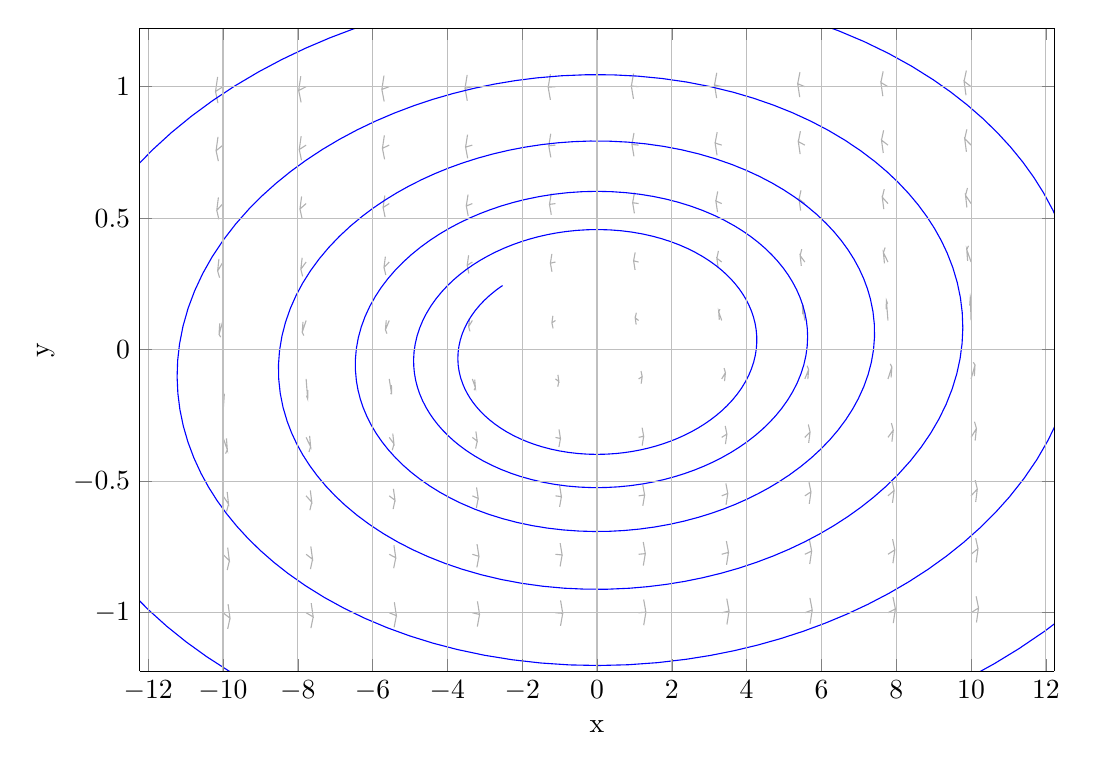
\begin{tikzpicture}

\begin{axis}[%
width=4.571659in,
height=3.214906in,
at={(0.866319in,1.696914in)},
scale only axis,
unbounded coords=jump,
separate axis lines,
every outer x axis line/.append style={black},
every x tick label/.append style={font=\color{black}},
xmin=-12.2222222222222,
xmax=12.2222222222222,
xlabel={x},
xmajorgrids,
every outer y axis line/.append style={black},
every y tick label/.append style={font=\color{black}},
ymin=-1.22222222222222,
ymax=1.22222222222222,
ylabel={y},
ymajorgrids,
every outer z axis line/.append style={black},
every z tick label/.append style={font=\color{black}},
zmin=-1,
zmax=1,
view={0}{90}
]
\addplot [color=white!70!black,solid,forget plot]
  table[row sep=crcr]{%
-10	-1\\
-9.81241194585928	-1.02056435585844\\
-9.86354727313689	-0.967498035565731\\
-9.81241194585928	-1.02056435585844\\
-9.87382945106611	-1.06129206263609\\
nan	0\\
-10	-0.777777777777778\\
-9.82958536756474	-0.802476346039514\\
-9.87453511522989	-0.752463117452179\\
-9.82958536756474	-0.802476346039514\\
-9.88688439936075	-0.837670433669807\\
nan	0\\
-10	-0.555555555555556\\
-9.85148358196474	-0.587306416934181\\
-9.88810079203066	-0.540652054011778\\
-9.85148358196474	-0.587306416934181\\
-9.90397622271997	-0.614910263029409\\
nan	0\\
-10	-0.333333333333333\\
-9.88446219903126	-0.380389184936132\\
-9.90735957642118	-0.337387979213108\\
-9.88446219903126	-0.380389184936132\\
-9.93088750222258	-0.395156879697477\\
nan	0\\
-10	-0.111111111111111\\
-9.97935536744191	-0.199672451922752\\
-9.96340842200643	-0.167942891539737\\
-9.97935536744191	-0.199672451922752\\
-10.0076890924122	-0.178265207818783\\
nan	0\\
-10	0.111111111111111\\
-10.1051566362561	0.0582449661940668\\
-10.06039310915	0.0478156506051543\\
-10.1051566362561	0.0582449661940668\\
-10.0868261816085	0.100393968733206\\
nan	0\\
-10	0.333333333333333\\
-10.1429235188413	0.299395502359456\\
-10.0915620054455	0.273845971941289\\
-10.1429235188413	0.299395502359456\\
-10.1085309209324	0.34530773136195\\
nan	0\\
-10	0.555555555555555\\
-10.1663153217761	0.529704325960978\\
-10.1099579178447	0.495880864395318\\
-10.1663153217761	0.529704325960978\\
-10.1228835326419	0.579038525283385\\
nan	0\\
-10	0.777777777777778\\
-10.1842555048727	0.756490782015734\\
-10.1236571044704	0.716813004526161\\
-10.1842555048727	0.756490782015734\\
-10.1343006023514	0.808940756962533\\
nan	0\\
-10	1\\
-10.1991602309428	0.981691466175508\\
-10.1348350282039	0.937393968587151\\
-10.1991602309428	0.981691466175508\\
-10.1439892951161	1.03697408405856\\
nan	0\\
-7.77777777777778	-1\\
-7.58854648285336	-1.01579673079962\\
-7.64136668863078	-0.963749887828626\\
-7.58854648285336	-1.01579673079962\\
-7.64926505403059	-1.05836553529084\\
nan	0\\
-7.77777777777778	-0.777777777777778\\
-7.6052640385214	-0.796689610627632\\
-7.65229020208585	-0.747887625958583\\
-7.6052640385214	-0.796689610627632\\
-7.66174611851078	-0.834144495586769\\
nan	0\\
-7.77777777777778	-0.555555555555556\\
-7.62624106257134	-0.57974393076523\\
-7.66565498333085	-0.534603239400719\\
-7.62624106257134	-0.57974393076523\\
-7.67774917093569	-0.610371597003936\\
nan	0\\
-7.77777777777778	-0.333333333333333\\
-7.65642428325531	-0.368944738617867\\
-7.68392748029092	-0.32792294340189\\
-7.65642428325531	-0.368944738617867\\
-7.70173318293318	-0.388599690663124\\
nan	0\\
-7.77777777777778	-0.111111111111111\\
-7.73599401236168	-0.187002745234794\\
-7.72955623345559	-0.153789313643665\\
-7.73599401236168	-0.187002745234794\\
-7.76750205051743	-0.174681196351713\\
nan	0\\
-7.77777777777778	0.111111111111111\\
-7.88119146430226	0.0662767369211356\\
-7.83895876479742	0.0538736275470088\\
-7.88119146430226	0.0662767369211356\\
-7.86137595189241	0.105580470809248\\
nan	0\\
-7.77777777777778	0.333333333333333\\
-7.91930735036248	0.305924850843073\\
-7.86999635796451	0.278765002443974\\
-7.91930735036248	0.305924850843073\\
-7.88370059920964	0.349529788736328\\
nan	0\\
-7.77777777777778	0.555555555555555\\
-7.94285876749928	0.534974090659561\\
-7.88818910435883	0.499878282697984\\
-7.94285876749928	0.534974090659561\\
-7.89847983680683	0.582418777558734\\
nan	0\\
-7.77777777777778	0.777777777777778\\
-7.96093376981838	0.760940492243617\\
-7.90177765082266	0.720202679893716\\
-7.96093376981838	0.760940492243617\\
-7.91019629358974	0.811780675914015\\
nan	0\\
-7.77777777777778	1\\
-7.97594664526146	0.985572129132925\\
-7.91288901729959	0.940358273522127\\
-7.97594664526146	0.985572129132925\\
-7.92010295273312	1.03944270726397\\
nan	0\\
-5.55555555555556	-1\\
-5.36478754435193	-1.01114168970936\\
-5.41923252528567	-0.960107179995643\\
-5.36478754435193	-1.01114168970936\\
-5.42480337014035	-1.05549118559746\\
nan	0\\
-5.55555555555556	-0.777777777777778\\
-5.38111717280357	-0.791071359758572\\
-5.43012529213397	-0.743473689476337\\
-5.38111717280357	-0.791071359758572\\
-5.43677208312436	-0.830692880852331\\
nan	0\\
-5.55555555555556	-0.555555555555556\\
-5.40134491418156	-0.572460909795196\\
-5.44338176803385	-0.528836643179804\\
-5.40134491418156	-0.572460909795196\\
-5.45183444515367	-0.605941963866804\\
nan	0\\
-5.55555555555556	-0.333333333333333\\
-5.42940822002481	-0.357961864284279\\
-5.4610952879463	-0.319036471116309\\
-5.42940822002481	-0.357961864284279\\
-5.47340955342177	-0.382110138881682\\
nan	0\\
-5.55555555555556	-0.111111111111111\\
-5.49219165581084	-0.167585175054708\\
-5.49708230974836	-0.13480198093545\\
-5.49219165581084	-0.167585175054708\\
-5.52531934172015	-0.166483930807808\\
nan	0\\
-5.55555555555556	0.111111111111111\\
-5.65702691981853	0.0758535140774167\\
-5.61777111128121	0.0610629521217819\\
-5.65702691981853	0.0758535140774167\\
-5.63539990979806	0.111798634253268\\
nan	0\\
-5.55555555555556	0.333333333333333\\
-5.69549479662779	0.312987412851764\\
-5.64842654418572	0.284106378728178\\
-5.69549479662779	0.312987412851764\\
-5.65859950442651	0.354075999264293\\
nan	0\\
-5.55555555555556	0.555555555555555\\
-5.71927934431476	0.540504646495139\\
-5.6663994804219	0.504088972023462\\
-5.71927934431476	0.540504646495139\\
-5.67392493495211	0.585950866403066\\
nan	0\\
-5.55555555555556	0.777777777777778\\
-5.73752955813875	0.76554669815799\\
-5.67987958745885	0.723722521398127\\
-5.73752955813875	0.76554669815799\\
-5.68599512726874	0.814709522689726\\
nan	0\\
-5.55555555555556	1\\
-5.75267374583829	0.989558311776526\\
-5.6909278666976	0.943411270672884\\
-5.75267374583829	0.989558311776526\\
-5.69614871080934	1.04197036581425\\
nan	0\\
-3.33333333333333	-1\\
-3.14112720121187	-1.00660003200747\\
-3.19713903284644	-0.956568489374861\\
-3.14112720121187	-1.00660003200747\\
-3.20043904885017	-1.05267155543559\\
nan	0\\
-3.33333333333333	-0.777777777777778\\
-3.15712878001146	-0.785624668790538\\
-3.20802842325483	-0.739219463156243\\
-3.15712878001146	-0.785624668790538\\
-3.21195186876122	-0.827321739817177\\
nan	0\\
-3.33333333333333	-0.555555555555556\\
-3.17675451149172	-0.565472721149544\\
-3.22124886664571	-0.523352866010944\\
-3.17675451149172	-0.565472721149544\\
-3.2262074494427	-0.60164227693175\\
nan	0\\
-3.33333333333333	-0.333333333333333\\
-3.20326704106137	-0.347591861317543\\
-3.23872229674691	-0.310797729854289\\
-3.20326704106137	-0.347591861317543\\
-3.24585156073901	-0.375830875990272\\
nan	0\\
-3.33333333333333	-0.111111111111111\\
-3.25322389641798	-0.143737816344082\\
-3.26910005118434	-0.113922445545352\\
-3.25322389641798	-0.143737816344082\\
-3.28541340380083	-0.153977164003029\\
nan	0\\
-3.33333333333333	0.111111111111111\\
-3.43243096649183	0.0875799333783673\\
-3.39681888211109	0.0698648784085666\\
-3.43243096649183	0.0875799333783673\\
-3.40858447097747	0.119413694987814\\
nan	0\\
-3.33333333333333	0.333333333333333\\
-3.47142332485981	0.320638904989292\\
-3.42682272031586	0.289924735610884\\
-3.47142332485981	0.320638904989292\\
-3.43316993448788	0.358969731374125\\
nan	0\\
-3.33333333333333	0.555555555555555\\
-3.49555527909082	0.546309329973755\\
-3.44457713896812	0.508527711208924\\
-3.49555527909082	0.546309329973755\\
-3.44920025175902	0.589638684087667\\
nan	0\\
-3.33333333333333	0.777777777777778\\
-3.51403282093641	0.770314352070681\\
-3.45795711822871	0.727378507882042\\
-3.51403282093641	0.770314352070681\\
-3.46168883108226	0.817728251683579\\
nan	0\\
-3.33333333333333	1\\
-3.52933604019161	0.99365235096644\\
-3.46894831587574	0.946555968961938\\
-3.52933604019161	0.99365235096644\\
-3.47212214039252	1.04455732239108\\
nan	0\\
-1.11111111111111	-1\\
-0.917557876910838	-1.00217177839591\\
-0.975080902571942	-0.953131936327069\\
-0.917557876910838	-1.00217177839591\\
-0.976166791769897	-1.04990855342721\\
nan	0\\
-1.11111111111111	-0.777777777777778\\
-0.933283653772106	-0.78035043854192\\
-0.985988725782772	-0.735121775977926\\
-0.933283653772106	-0.78035043854192\\
-0.987275056164843	-0.824035504647428\\
nan	0\\
-1.11111111111111	-0.555555555555556\\
-0.952431041938794	-0.558785881461918\\
-0.999227481213899	-0.51814676639693\\
-0.952431041938794	-0.558785881461918\\
-1.00084264416708	-0.597486800983088\\
nan	0\\
-1.11111111111111	-0.333333333333333\\
-0.977842822405366	-0.337909539936786\\
-1.01667925736623	-0.303219605779314\\
-0.977842822405366	-0.337909539936786\\
-1.01896736066795	-0.369853750132186\\
nan	0\\
-1.11111111111111	-0.111111111111111\\
-1.02092818095136	-0.120997422244607\\
-1.04551148221591	-0.0954857963646205\\
-1.02092818095136	-0.120997422244607\\
-1.05045463778266	-0.140577261444496\\
nan	0\\
-1.11111111111111	0.111111111111111\\
-1.20685736361098	0.102309286097334\\
-1.17593303160757	0.0810132704764999\\
-1.20685736361098	0.102309286097334\\
-1.18033394411446	0.128886396726434\\
nan	0\\
-1.11111111111111	0.333333333333333\\
-1.24701179771454	0.328932119310293\\
-1.20514128822775	0.296277311866348\\
-1.24701179771454	0.328932119310293\\
-1.20734189523927	0.364227655168063\\
nan	0\\
-1.11111111111111	0.555555555555555\\
-1.27166140789588	0.55239996184541\\
-1.22270742043291	0.513209065762261\\
-1.27166140789588	0.55239996184541\\
-1.22428521728799	0.593484214154647\\
nan	0\\
-1.11111111111111	0.777777777777778\\
-1.29043246978954	0.775247777514248\\
-1.23600356212013	0.731176437923701\\
-1.29043246978954	0.775247777514248\\
-1.23726856225189	0.820837117262913\\
nan	0\\
-1.11111111111111	1\\
-1.30592761362348	0.997856285321944\\
-1.24694673420026	0.949795274097268\\
-1.30592761362348	0.997856285321944\\
-1.24801859153928	1.04720352535345\\
nan	0\\
1.11111111111111	-1\\
1.30592761362348	-0.997856285321944\\
1.24694673420026	-0.949795274097268\\
1.30592761362348	-0.997856285321944\\
1.24801859153928	-1.04720352535345\\
nan	0\\
1.11111111111111	-0.777777777777778\\
1.29043246978954	-0.775247777514249\\
1.23600356212013	-0.731176437923701\\
1.29043246978954	-0.775247777514249\\
1.23726856225189	-0.820837117262914\\
nan	0\\
1.11111111111111	-0.555555555555556\\
1.27166140789588	-0.55239996184541\\
1.22270742043291	-0.513209065762261\\
1.27166140789588	-0.55239996184541\\
1.22428521728799	-0.593484214154647\\
nan	0\\
1.11111111111111	-0.333333333333333\\
1.24701179771454	-0.328932119310293\\
1.20514128822775	-0.296277311866348\\
1.24701179771454	-0.328932119310293\\
1.20734189523927	-0.364227655168063\\
nan	0\\
1.11111111111111	-0.111111111111111\\
1.20685736361098	-0.102309286097334\\
1.17593303160757	-0.0810132704764999\\
1.20685736361098	-0.102309286097334\\
1.18033394411446	-0.128886396726434\\
nan	0\\
1.11111111111111	0.111111111111111\\
1.02092818095136	0.120997422244607\\
1.04551148221591	0.0954857963646205\\
1.02092818095136	0.120997422244607\\
1.05045463778266	0.140577261444496\\
nan	0\\
1.11111111111111	0.333333333333333\\
0.977842822405366	0.337909539936786\\
1.01667925736623	0.303219605779314\\
0.977842822405366	0.337909539936786\\
1.01896736066795	0.369853750132186\\
nan	0\\
1.11111111111111	0.555555555555555\\
0.952431041938794	0.558785881461917\\
0.999227481213899	0.51814676639693\\
0.952431041938794	0.558785881461917\\
1.00084264416708	0.597486800983088\\
nan	0\\
1.11111111111111	0.777777777777778\\
0.933283653772106	0.780350438541919\\
0.985988725782772	0.735121775977926\\
0.933283653772106	0.780350438541919\\
0.987275056164843	0.824035504647428\\
nan	0\\
1.11111111111111	1\\
0.917557876910838	1.00217177839591\\
0.975080902571942	0.953131936327069\\
0.917557876910838	1.00217177839591\\
0.976166791769897	1.04990855342721\\
nan	0\\
3.33333333333333	-1\\
3.52933604019161	-0.99365235096644\\
3.46894831587574	-0.946555968961938\\
3.52933604019161	-0.99365235096644\\
3.47212214039252	-1.04455732239108\\
nan	0\\
3.33333333333333	-0.777777777777778\\
3.51403282093641	-0.770314352070682\\
3.45795711822871	-0.727378507882042\\
3.51403282093641	-0.770314352070682\\
3.46168883108226	-0.817728251683579\\
nan	0\\
3.33333333333333	-0.555555555555556\\
3.49555527909082	-0.546309329973756\\
3.44457713896812	-0.508527711208924\\
3.49555527909082	-0.546309329973756\\
3.44920025175902	-0.589638684087667\\
nan	0\\
3.33333333333333	-0.333333333333333\\
3.47142332485981	-0.320638904989292\\
3.42682272031586	-0.289924735610884\\
3.47142332485981	-0.320638904989292\\
3.43316993448788	-0.358969731374125\\
nan	0\\
3.33333333333333	-0.111111111111111\\
3.43243096649183	-0.0875799333783673\\
3.39681888211109	-0.0698648784085666\\
3.43243096649183	-0.0875799333783673\\
3.40858447097747	-0.119413694987814\\
nan	0\\
3.33333333333333	0.111111111111111\\
3.25322389641798	0.143737816344082\\
3.26910005118434	0.113922445545352\\
3.25322389641798	0.143737816344082\\
3.28541340380083	0.153977164003029\\
nan	0\\
3.33333333333333	0.333333333333333\\
3.20326704106137	0.347591861317543\\
3.23872229674691	0.310797729854289\\
3.20326704106137	0.347591861317543\\
3.24585156073901	0.375830875990272\\
nan	0\\
3.33333333333333	0.555555555555555\\
3.17675451149172	0.565472721149543\\
3.22124886664571	0.523352866010944\\
3.17675451149172	0.565472721149543\\
3.2262074494427	0.60164227693175\\
nan	0\\
3.33333333333333	0.777777777777778\\
3.15712878001147	0.785624668790538\\
3.20802842325484	0.739219463156243\\
3.15712878001147	0.785624668790538\\
3.21195186876122	0.827321739817177\\
nan	0\\
3.33333333333333	1\\
3.14112720121187	1.00660003200747\\
3.19713903284644	0.956568489374861\\
3.14112720121187	1.00660003200747\\
3.20043904885018	1.05267155543559\\
nan	0\\
5.55555555555556	-1\\
5.75267374583829	-0.989558311776526\\
5.6909278666976	-0.943411270672884\\
5.75267374583829	-0.989558311776526\\
5.69614871080934	-1.04197036581425\\
nan	0\\
5.55555555555556	-0.777777777777778\\
5.73752955813876	-0.76554669815799\\
5.67987958745885	-0.723722521398127\\
5.73752955813876	-0.76554669815799\\
5.68599512726874	-0.814709522689726\\
nan	0\\
5.55555555555556	-0.555555555555556\\
5.71927934431477	-0.540504646495139\\
5.6663994804219	-0.504088972023462\\
5.71927934431477	-0.540504646495139\\
5.67392493495211	-0.585950866403066\\
nan	0\\
5.55555555555556	-0.333333333333333\\
5.69549479662779	-0.312987412851765\\
5.64842654418573	-0.284106378728178\\
5.69549479662779	-0.312987412851765\\
5.65859950442651	-0.354075999264293\\
nan	0\\
5.55555555555556	-0.111111111111111\\
5.65702691981853	-0.0758535140774167\\
5.61777111128121	-0.0610629521217819\\
5.65702691981853	-0.0758535140774167\\
5.63539990979806	-0.111798634253268\\
nan	0\\
5.55555555555556	0.111111111111111\\
5.49219165581084	0.167585175054708\\
5.49708230974836	0.13480198093545\\
5.49219165581084	0.167585175054708\\
5.52531934172016	0.166483930807808\\
nan	0\\
5.55555555555556	0.333333333333333\\
5.42940822002481	0.357961864284279\\
5.4610952879463	0.319036471116309\\
5.42940822002481	0.357961864284279\\
5.47340955342177	0.382110138881681\\
nan	0\\
5.55555555555556	0.555555555555555\\
5.40134491418156	0.572460909795196\\
5.44338176803385	0.528836643179804\\
5.40134491418156	0.572460909795196\\
5.45183444515367	0.605941963866804\\
nan	0\\
5.55555555555556	0.777777777777778\\
5.38111717280357	0.791071359758572\\
5.43012529213397	0.743473689476337\\
5.38111717280357	0.791071359758572\\
5.43677208312436	0.830692880852331\\
nan	0\\
5.55555555555556	1\\
5.36478754435193	1.01114168970936\\
5.41923252528568	0.960107179995643\\
5.36478754435193	1.01114168970936\\
5.42480337014036	1.05549118559746\\
nan	0\\
7.77777777777778	-1\\
7.97594664526146	-0.985572129132925\\
7.91288901729959	-0.940358273522127\\
7.97594664526146	-0.985572129132925\\
7.92010295273312	-1.03944270726397\\
nan	0\\
7.77777777777778	-0.777777777777778\\
7.96093376981838	-0.760940492243617\\
7.90177765082266	-0.720202679893716\\
7.96093376981838	-0.760940492243617\\
7.91019629358974	-0.811780675914015\\
nan	0\\
7.77777777777778	-0.555555555555556\\
7.94285876749928	-0.534974090659561\\
7.88818910435883	-0.499878282697984\\
7.94285876749928	-0.534974090659561\\
7.89847983680683	-0.582418777558735\\
nan	0\\
7.77777777777778	-0.333333333333333\\
7.91930735036249	-0.305924850843073\\
7.86999635796451	-0.278765002443974\\
7.91930735036249	-0.305924850843073\\
7.88370059920964	-0.349529788736328\\
nan	0\\
7.77777777777778	-0.111111111111111\\
7.88119146430226	-0.0662767369211356\\
7.83895876479742	-0.0538736275470088\\
7.88119146430226	-0.0662767369211356\\
7.86137595189241	-0.105580470809248\\
nan	0\\
7.77777777777778	0.111111111111111\\
7.73599401236168	0.187002745234794\\
7.72955623345559	0.153789313643665\\
7.73599401236168	0.187002745234794\\
7.76750205051743	0.174681196351713\\
nan	0\\
7.77777777777778	0.333333333333333\\
7.65642428325531	0.368944738617867\\
7.68392748029092	0.32792294340189\\
7.65642428325531	0.368944738617867\\
7.70173318293319	0.388599690663124\\
nan	0\\
7.77777777777778	0.555555555555555\\
7.62624106257134	0.579743930765229\\
7.66565498333086	0.534603239400719\\
7.62624106257134	0.579743930765229\\
7.67774917093569	0.610371597003936\\
nan	0\\
7.77777777777778	0.777777777777778\\
7.60526403852141	0.796689610627632\\
7.65229020208585	0.747887625958582\\
7.60526403852141	0.796689610627632\\
7.66174611851078	0.834144495586769\\
nan	0\\
7.77777777777778	1\\
7.58854648285336	1.01579673079962\\
7.64136668863078	0.963749887828626\\
7.58854648285336	1.01579673079962\\
7.64926505403059	1.05836553529084\\
nan	0\\
10	-1\\
10.1991602309428	-0.981691466175508\\
10.1348350282039	-0.937393968587151\\
10.1991602309428	-0.981691466175508\\
10.1439892951161	-1.03697408405856\\
nan	0\\
10	-0.777777777777778\\
10.1842555048727	-0.756490782015735\\
10.1236571044704	-0.716813004526161\\
10.1842555048727	-0.756490782015735\\
10.1343006023514	-0.808940756962534\\
nan	0\\
10	-0.555555555555556\\
10.1663153217761	-0.529704325960978\\
10.1099579178447	-0.495880864395318\\
10.1663153217761	-0.529704325960978\\
10.1228835326419	-0.579038525283385\\
nan	0\\
10	-0.333333333333333\\
10.1429235188413	-0.299395502359456\\
10.0915620054455	-0.273845971941289\\
10.1429235188413	-0.299395502359456\\
10.1085309209324	-0.34530773136195\\
nan	0\\
10	-0.111111111111111\\
10.1051566362561	-0.0582449661940668\\
10.06039310915	-0.0478156506051543\\
10.1051566362561	-0.0582449661940668\\
10.0868261816085	-0.100393968733206\\
nan	0\\
10	0.111111111111111\\
9.97935536744191	0.199672451922752\\
9.96340842200643	0.167942891539737\\
9.97935536744191	0.199672451922752\\
10.0076890924122	0.178265207818783\\
nan	0\\
10	0.333333333333333\\
9.88446219903126	0.380389184936132\\
9.90735957642118	0.337387979213108\\
9.88446219903126	0.380389184936132\\
9.93088750222258	0.395156879697477\\
nan	0\\
10	0.555555555555555\\
9.85148358196474	0.587306416934181\\
9.88810079203066	0.540652054011777\\
9.85148358196474	0.587306416934181\\
9.90397622271997	0.614910263029409\\
nan	0\\
10	0.777777777777778\\
9.82958536756474	0.802476346039514\\
9.87453511522989	0.752463117452179\\
9.82958536756474	0.802476346039514\\
9.88688439936075	0.837670433669807\\
nan	0\\
10	1\\
9.81241194585928	1.02056435585844\\
9.86354727313689	0.967498035565731\\
9.81241194585928	1.02056435585844\\
9.87382945106611	1.06129206263609\\
nan	0\\
};
\addplot3 [color=blue,solid]
 table[row sep=crcr] {%
-2.52463885513703	0.243956531381681	0\\
-2.54953737148386	0.241573134930288	0.00093941572513655\\
-2.57423134515417	0.239166444273283	0.0018788314502731\\
-2.59871842594613	0.236736652744317	0.00281824717540965\\
-2.62299628079593	0.234283955824116	0.0037576629005462\\
-2.64706259377769	0.231808551140481	0.00469707862568275\\
-2.67091506610354	0.229310638468288	0.0056364943508193\\
-2.69455141612358	0.226790419729493	0.00657591007595585\\
-2.71796937932587	0.224248098993123	0.0075153258010924\\
-2.87093750186743	0.206430280681934	0.0138892881847653\\
-3.01308353242483	0.187671510045082	0.0202632505684381\\
-3.14374765124357	0.168043579318806	0.026637212952111\\
-3.26232466213577	0.147621573462762	0.0330111753357839\\
-3.36826399248022	0.126483870160022	0.0393851377194568\\
-3.46106969322239	0.104712139817074	0.0457591001031296\\
-3.54030043887437	0.0823913455638228	0.0521330624868025\\
-3.60556952751492	0.0596097432535889	0.0585070248704754\\
-3.65674854854113	0.0363468895394741	0.0649109798562709\\
-3.69319267624266	0.0128026281744376	0.0713149348420665\\
-3.71465353409658	-0.0109262044812335	0.077718889827862\\
-3.7209504564399	-0.0347426366653714	0.0841228448136576\\
-3.71197048846954	-0.058549561213928	0.0905267997994531\\
-3.68766838624232	-0.0822497355609748	0.0969307547852487\\
-3.64806661667503	-0.105745781738703	0.103334709771044\\
-3.59325535754434	-0.128940186377423	0.10973866475684\\
-3.53749851312201	-0.14753326109541	0.11495217130921\\
-3.47185230948046	-0.165810243656967	0.12016567786158\\
-3.39644856418335	-0.183719105734031	0.12537918441395\\
-3.31144648215976	-0.20120908967568	0.13059269096632\\
-3.21703265570418	-0.218230708508127	0.13580619751869\\
-3.11342106447648	-0.234735745934728	0.14101970407106\\
-3.00085307550193	-0.250677256335975	0.14623321062343\\
-2.8795974431712	-0.266009564769501	0.1514467171758\\
-2.73496906640253	-0.282284423132991	0.157241947558176\\
-2.5803964009829	-0.297692900951248	0.163037177940551\\
-2.41635155660908	-0.312177355604101	0.168832408322927\\
-2.24333786526468	-0.325683759822201	0.174627638705302\\
-2.06188988122023	-0.338161701687018	0.180422869087678\\
-1.87257338103308	-0.349564384630844	0.186218099470053\\
-1.6759853635475	-0.359848627436792	0.192013329852428\\
-1.47275404989459	-0.368974864238796	0.197808560234804\\
-1.24026992139891	-0.377702432745986	0.204238510846364\\
-1.00132286913168	-0.384915162046602	0.210668461457923\\
-0.756880311784414	-0.390572688852038	0.217098412069483\\
-0.507927242639707	-0.39464184138227	0.223528362681043\\
-0.255466229571245	-0.397096639365854	0.229958313292602\\
-0.000517415043803648	-0.397918294039927	0.236388263904162\\
0.255881483886752	-0.397095208150209	0.242818214515722\\
0.512675175573474	-0.394622975951	0.249248165127282\\
0.728051775887023	-0.391270089216833	0.254652781745618\\
0.942326705630462	-0.386756187228877	0.260057398363955\\
1.15485799175283	-0.381088613766554	0.265462014982292\\
1.36501198754741	-0.374278238980948	0.270866631600629\\
1.57216337265174	-0.366339459394804	0.276271248218966\\
1.77569515304762	-0.357290197902528	0.281675864837303\\
1.97499866106106	-0.347151903770187	0.28708048145564\\
2.16947355536236	-0.33594955263551	0.292485098073977\\
2.35623358732023	-0.323868243679008	0.297822949387578\\
2.53714879569578	-0.310805468894792	0.303160800701179\\
2.71166533402786	-0.296794005001333	0.30849865201478\\
2.8792510552048	-0.281869335907071	0.313836503328381\\
3.0393955114644	-0.266069652710418	0.319174354641982\\
3.19160995439394	-0.249435853699758	0.324512205955584\\
3.33542733493016	-0.232011544353442	0.329850057269185\\
3.47040230335928	-0.213843037339796	0.335187908582786\\
3.61416004235552	-0.192090168523607	0.341326815907968\\
3.74505296214502	-0.169493719262271	0.347465723233149\\
3.86249878011785	-0.146135404991408	0.353604630558331\\
3.96597306874113	-0.122099493172007	0.359743537883513\\
4.055009255559	-0.0974728032904351	0.365882445208694\\
4.12919862319264	-0.072344706858429	0.372021352533876\\
4.18819030934024	-0.0468071274131004	0.378160259859057\\
4.23169130677705	-0.0209545405169332	0.384299167184239\\
4.2580712590717	0.00333609511056443	0.390019732919852\\
4.27062401230471	0.0277387196872827	0.395740298655465\\
4.26923027485969	0.0521726547075702	0.401460864391079\\
4.25381984529303	0.0765575417634933	0.407181430126692\\
4.2243716123339	0.100813342544836	0.412901995862305\\
4.18091355488423	0.1248603388391	0.418622561597918\\
4.12352274201875	0.148619132531505	0.424343127333531\\
4.05232533298495	0.172010645604989	0.430063693069144\\
3.9787313005877	0.192140749170099	0.435075523518222\\
3.89479990435716	0.211876457286547	0.440087353967299\\
3.80069580327496	0.231165598145863	0.445099184416376\\
3.69660987515563	0.249957372712364	0.450111014865454\\
3.58275921664664	0.268202354723152	0.455122845314531\\
3.45938714322839	0.285852490688118	0.460134675763608\\
3.32676318921417	0.302861099889936	0.465146506212686\\
3.18518310775021	0.31918287438407	0.470158336661763\\
3.00795439468882	0.337410896808102	0.476042580715478\\
2.81936808959254	0.354563369136315	0.481926824769194\\
2.62002360626585	0.370573526666975	0.487811068822909\\
2.41055659059686	0.385379195936704	0.493695312876624\\
2.19163892055738	0.398922794720484	0.49957955693034\\
1.96397870620289	0.41115133203165	0.505463800984055\\
1.72832028967254	0.422016408121895	0.51134804503777\\
1.48544424518916	0.431474214481271	0.517232289091486\\
1.21036192340659	0.440221183032222	0.523717366640754\\
0.928597675959549	0.447163479368953	0.530202444190022\\
0.641318758376293	0.45225934008511	0.536687521739291\\
0.349708955064771	0.455475651364104	0.543172599288559\\
0.0549685793126407	0.456787948979118	0.549657676837828\\
-0.241685526712736	0.456180418293104	0.556142754387096\\
-0.539019991964293	0.453645894258782	0.562627831936365\\
-0.835784916515264	0.449185861418642	0.569112909485633\\
-1.0801310939543	0.444042666077613	0.574481366189135\\
-1.3225179323629	0.437592974688615	0.579849822892637\\
-1.56222532421052	0.429848916854006	0.585218279596139\\
-1.79854456138531	0.420826506262126	0.590586736299641\\
-2.03077833519408	0.410545640687297	0.595955193003143\\
-2.25824073636236	0.399030101989818	0.601323649706645\\
-2.48025725503432	0.386307556115973	0.606692106410146\\
-2.69616478077284	0.372409553098023	0.612060563113648\\
-2.90909737484152	0.357083617291038	0.617527736543755\\
-3.11434774240454	0.340614312495133	0.622994909973862\\
-3.31125140418673	0.323045641339808	0.628462083403968\\
-3.49917340591627	0.304424873187658	0.633929256834075\\
-3.6775083183247	0.284802544134369	0.639396430264182\\
-3.8456802371469	0.264232457008719	0.644863603694289\\
-4.00314278312111	0.24277168137258	0.650330777124395\\
-4.1493791019889	0.220480553520914	0.655797950554502\\
-4.30138347266504	0.194209297836297	0.662013312356874\\
-4.43757638684455	0.167041697254854	0.668228674159246\\
-4.55732215685077	0.139079292614893	0.674444035961618\\
-4.66005724091033	0.110426249090555	0.68065939776399\\
-4.74529024315323	0.0811893561918218	0.686874759566362\\
-4.81260191361277	0.0514780277645118	0.693090121368734\\
-4.86164514822559	0.0214043019902807	0.699305483171106\\
-4.89214498883165	-0.00891715861337908	0.705520844973478\\
-4.90345962977691	-0.0356155959869364	0.710970421242432\\
-4.90023965023054	-0.0623366841666692	0.716419997511386\\
-4.88241814227239	-0.0889998586991246	0.72186957378034\\
-4.84997435484199	-0.115525114799782	0.727319150049294\\
-4.8029336937386	-0.141833007353052	0.732768726318248\\
-4.74136772162114	-0.167844650912278	0.738218302587202\\
-4.66539415800825	-0.193481719699734	0.743667878856156\\
-4.57517687927826	-0.218666447606629	0.74911745512511\\
-4.48002780884107	-0.241313713763144	0.754118264957009\\
-4.37323505382051	-0.263456436462847	0.759119074788909\\
-4.25501424674027	-0.285036042603881	0.764119884620808\\
-4.12561022761644	-0.305995655072633	0.769120694452708\\
-3.98529704395749	-0.326280092743741	0.774121504284607\\
-3.83437795076429	-0.345835870480088	0.779122314116507\\
-3.67318541053011	-0.364611199132803	0.784123123948406\\
-3.50208109324059	-0.382555985541264	0.789123933780306\\
-3.2857589370373	-0.40279067879689	0.795083563795009\\
-3.05660320166021	-0.421698802355246	0.801043193809713\\
-2.81536781006231	-0.439204064421199	0.807002823824416\\
-2.56284797294821	-0.455235932834348	0.81296245383912\\
-2.29988018877408	-0.469729635069017	0.818922083853823\\
-2.02734224374768	-0.482626158234261	0.824881713868527\\
-1.74615321182836	-0.493872249073861	0.83084134388323\\
-1.45727345472705	-0.503420413966331	0.836800973897934\\
-1.13243096622625	-0.511898489576752	0.843343768968266\\
-0.800846502565246	-0.518230196439062	0.849886564038599\\
-0.463926513581075	-0.522373472657226	0.856429359108931\\
-0.123091691784856	-0.524296647442224	0.862972154179264\\
0.220223027638204	-0.523978441112045	0.869514949249596\\
0.564568466828807	-0.521407965091686	0.876057744319928\\
0.908481205253567	-0.516584721913158	0.882600539390261\\
1.25048357970502	-0.509518605215481	0.889143334460593\\
1.52685136182108	-0.502110892701279	0.894477071976976\\
1.80017017740532	-0.493237207586073	0.89981080949336\\
2.0696342615021	-0.482915674745765	0.905144547009743\\
2.33445299128273	-0.471168685433431	0.910478284526126\\
2.5938508860454	-0.458022897279325	0.91581202204251\\
2.84706760721524	-0.443509234290877	0.921145759558893\\
3.09335795834426	-0.427662886852689	0.926479497075276\\
3.33199188511143	-0.410523311726544	0.931813234591659\\
3.57296731548468	-0.391230423439519	0.937400006255398\\
3.80396052730072	-0.370618832041845	0.942986777919136\\
4.0241836855056	-0.348746821402461	0.948573549582874\\
4.23288851141038	-0.325676551678942	0.954160321246612\\
4.42936628269115	-0.301474059317501	0.959747092910351\\
4.61294783338905	-0.276209257052983	0.965333864574089\\
4.78300355391024	-0.249955933908872	0.970920636237827\\
4.93894339102594	-0.222791755197286	0.976507407901565\\
5.09695909764897	-0.191214261779277	0.982798072832153\\
5.2356469506793	-0.158702605364944	0.989088737762741\\
5.35432398752309	-0.125382248726769	0.995379402693329\\
5.45239668617473	-0.0913812425908319	1.00167006762392\\
5.52936096521684	-0.0568302256368078	1.0079607325545\\
5.58480218382025	-0.0218624244979693	1.01425139748509\\
5.61839514174403	0.0133863462388142	1.02054206241568\\
5.62990407933544	0.0487776840330781	1.02683272734627\\
5.62203885895981	0.0791744564792287	1.03223416376666\\
5.59770332674167	0.10948492986247	1.03763560018704\\
5.55688376384794	0.139618763786658	1.04303703660743\\
5.49961731935771	0.169486576154884	1.04843847302782\\
5.42599201026228	0.198999943169474	1.05383990944821\\
5.33614672146511	0.228071399331993	1.0592413458686\\
5.23027120578187	0.256614437443239	1.06464278228899\\
5.10860608394038	0.284543508603249	1.07004421870937\\
4.97633356131725	0.310863992906032	1.0752625459558\\
4.82987567839244	0.336457776915644	1.08048087320223\\
4.66956654150022	0.361250448835276	1.08569920044866\\
4.49577859503672	0.385170205660132	1.09091752769508\\
4.30892262145996	0.408147853177434	1.09613585494151\\
4.10944774128986	0.43011680596642	1.10135418218794\\
3.89784141310818	0.451013087398344	1.10657250943437\\
3.6746294335586	0.470775329636476	1.1117908366808\\
3.40108260051971	0.492262265885678	1.11786162768086\\
3.11350670569581	0.512047037949123	1.12393241868093\\
2.81289795512307	0.530044977352055	1.13000320968099\\
2.50029770423504	0.546178968513058	1.13607400068106\\
2.1767924578627	0.560379448744062	1.14214479168112\\
1.84351387023446	0.572584408250339	1.14821558268119\\
1.50163874497611	0.582739390130504	1.15428637368126\\
1.15238903511087	0.590797490376516	1.16035716468132\\
0.774401234740981	0.597020414278004	1.16681097735645\\
0.391018877244034	0.600787465808141	1.17326479003157\\
0.00383870456758495	0.602066497087122	1.17971860270669\\
-0.385536914574306	0.600836724898174	1.18617241538182\\
-0.775499984701076	0.597088730687549	1.19262622805694\\
-1.16443688356565	0.590824460564531	1.19908004073206\\
-1.55072836215446	0.582057225301431	1.20553385340719\\
-1.93274954468742	0.570811700333588	1.21198766608231\\
-2.23880098516255	0.559875774153527	1.21722994404303\\
-2.54010623989631	0.547347783612344	1.22247222200376\\
-2.83580043306064	0.533254693590891	1.22771449996448\\
-3.12503859556705	0.517627887513325	1.23295677792521\\
-3.40699566506663	0.50050316734712	1.23819905588593\\
-3.68086648595004	0.48192075360306	1.24344133384665\\
-3.94586580934751	0.461925285335244	1.24868361180738\\
-4.20122829312885	0.44056582014108	1.2539258897681\\
-4.46912041172518	0.415655585448098	1.25967044428071\\
-4.7235981794682	0.389244507514765	1.26541499879333\\
-4.9637309276595	0.361412881399265	1.27115955330594\\
-5.18864326647325	0.332245549745374	1.27690410781855\\
-5.3975150849562	0.301831902782459	1.28264866233117\\
-5.58958155102767	0.270265878325481	1.28839321684378\\
-5.76413311147957	0.237645961774991	1.29413777135639\\
-5.92051549197638	0.204075186117134	1.299882325869\\
-6.07250831957859	0.165714183359902	1.30627713805909\\
-6.20048224308383	0.12645675833523	1.31267195024917\\
-6.303746912819	0.0864611352388039	1.31906676243925\\
-6.38172526307845	0.0458876759251402	1.32546157462933\\
-6.43395351212402	0.00489887990758892	1.33185638681941\\
-6.46008116218502	-0.036340615641668	1.3382511990095\\
-6.45987099945826	-0.0776640358916159	1.34464601119958\\
-6.43319909410797	-0.118902468352409	1.35104082338966\\
-6.3906272033124	-0.153150048186647	1.35638059839411\\
-6.32959934844859	-0.187121762939165	1.36172037339856\\
-6.2501974584375	-0.220717763370481	1.36706014840301\\
-6.15255839005245	-0.253839774536682	1.37239992340746\\
-6.03687392791903	-0.286391095789431	1.37773969841192\\
-5.90339078451516	-0.318276600775966	1.38307947341637\\
-5.7524106001711	-0.349402737439093	1.38841924842082\\
-5.5842899430694	-0.379677528017196	1.39375902342527\\
-5.39484430476572	-0.409695163550463	1.39922544894041\\
-5.18833259126714	-0.438631352493332	1.40469187445556\\
-4.96529195461284	-0.466392450380913	1.4101582999707\\
-4.72630923654709	-0.492888968660615	1.41562472548585\\
-4.47202096851926	-0.518035574692146	1.42109115100099\\
-4.20311337168382	-0.54175109174751	1.42655757651614\\
-3.92032235690035	-0.563958499011011	1.43202400203128\\
-3.6244335247335	-0.584584931579251	1.43749042754643\\
-3.27323947734976	-0.606024609299606	1.44370391169096\\
-2.90745082944039	-0.625238112288525	1.4499173958355\\
-2.52841813561522	-0.642135840254608	1.45613087998003\\
-2.13753787772163	-0.65663834524016	1.46234436412456\\
-1.73625246484452	-0.668676331621196	1.4685578482691\\
-1.3260502333063	-0.678190656107438	1.47477133241363\\
-0.908465446666925	-0.685132327742314	1.48098481655816\\
-0.485078295723864	-0.68946250790296	1.48719830070269\\
-0.0823042790979306	-0.691125916687632	1.49305234726862\\
0.322838983398461	-0.690424975978886	1.49890639383454\\
0.728950576029773	-0.68734849164594	1.50476044040046\\
1.13463394379846	-0.681893994450682	1.51061448696638\\
1.53849689244495	-0.674067740047676	1.5164685335323\\
1.93915158844768	-0.663884708984158	1.52232258009822\\
2.33521455902307	-0.651368606700039	1.52817662666414\\
2.72530669212553	-0.636551863527901	1.53403067323006\\
3.05568570915643	-0.621965493416638	1.53907616331742\\
3.37974409875082	-0.605727979124974	1.54412165340477\\
3.69661443656387	-0.587873337944721	1.54916714349213\\
4.00545182470155	-0.568439783073034	1.55421263357949\\
4.30543389172056	-0.547469723612406	1.55925812366684\\
4.59576079262842	-0.525009764570673	1.5643036137542\\
4.87565520888341	-0.501110706861014	1.56934910384156\\
5.14436234839459	-0.475827547301945	1.57439459392892\\
5.44177656662719	-0.444766634101765	1.58026116104664\\
5.72197069084942	-0.412010814855438	1.58612772816436\\
5.98386252380373	-0.377665150115029	1.59199429528208\\
6.22644303097867	-0.34183992843919	1.5978608623998\\
6.44877634060887	-0.304650666393161	1.60372742951752\\
6.64999974367505	-0.266218108548766	1.60959399663524\\
6.82932369390403	-0.226668227484417	1.61546056375296\\
6.9860318077687	-0.186132223785111	1.62132713087068\\
7.13194739077126	-0.140416425258992	1.62780084306816\\
7.24875372667252	-0.0938486153146721	1.63427455526565\\
7.33575866567383	-0.0466226750675951	1.64074826746313\\
7.39240927445341	0.0010659401770956	1.64722197966061\\
7.41829183616633	0.0490202009245581	1.6536956918581\\
7.41313185044453	0.0970415034902513	1.66016940405558\\
7.37679403339684	0.144929669999935	1.66664311625307\\
7.30928231760891	0.192482948389671	1.67311682845055\\
7.23096001557147	0.230989216768199	1.67841189481341\\
7.13196032206585	0.269026831837128	1.68370696117628\\
7.01246000748691	0.306485059062228	1.68900202753914\\
6.8726956951557	0.343255358250338	1.69429709390201\\
6.71296386131948	0.379231383549362	1.69959216026487\\
6.53362083515169	0.414308983448276	1.70488722662773\\
6.33508279875199	0.448386200777122	1.7101822929906\\
6.11782578714619	0.481363272707012	1.71547735935346\\
5.86697312913968	0.515099773697118	1.72110534075919\\
5.59625394206166	0.547369609859529	1.72673332216492\\
5.30643181102717	0.578060714849136	1.73236130357065\\
4.99833057370882	0.607066895048946	1.73798928497638\\
4.67283432033674	0.634287829570081	1.74361726638211\\
4.33088739369865	0.659629070251776	1.74924524778785\\
3.97349438913982	0.683002041661383	1.75487322919358\\
3.60172015456305	0.704324041094369	1.76050121059931\\
3.16870830355461	0.725717612934557	1.7668175621919\\
2.72060632280285	0.744330025211493	1.7731339137845\\
2.25914395195512	0.76006771268084	1.7794502653771\\
1.78609636241945	0.772850039588954	1.78576661696969\\
1.3032841573646	0.782609299672881	1.79208296856229\\
0.812573371720026	0.789290716160358	1.79839932015489\\
0.315875472175895	0.792852441769813	1.80471567174748\\
-0.184852642816931	0.793265558710366	1.81103202334008\\
-0.620397685527848	0.791063521530621	1.81650420954154\\
-1.05618854490361	0.786477623949286	1.821976395743\\
-1.4908995674507	0.779509196725716	1.82744858194445\\
-1.92321480455029	0.770167109374572	1.83292076814591\\
-2.35182801245825	0.758467770165823	1.83839295434737\\
-2.77544265230519	0.744435126124746	1.84386514054882\\
-3.19277189009639	0.728100663031926	1.84933732675028\\
-3.60253859671186	0.709503405423253	1.85480951295174\\
-3.97069740335034	0.690492399221125	1.85982921843037\\
-4.33046523087744	0.669654173747204	1.86484892390901\\
-4.68088230970327	0.647033283435818	1.86986862938765\\
-5.02101721595129	0.622678833292475	1.87488833486628\\
-5.34996687145831	0.59664447889386	1.87990804034492\\
-5.66685654377449	0.568988426387834	1.88492774582356\\
-5.97083984616335	0.539773432493437	1.88994745130219\\
-6.26109873760173	0.509066804500887	1.89496715678083\\
-6.58737753736975	0.470701305130512	1.90093736618176\\
-6.89185643833642	0.430452097139635	1.90690757558269\\
-7.17330004719471	0.388454287764456	1.91287778498361\\
-7.43056779971555	0.344848829155739	1.91884799438454\\
-7.66261396074784	0.29978251837881	1.92481820378547\\
-7.86848762421841	0.25340799741356	1.9307884131864\\
-8.04733271313209	0.20588375315444	1.93675862258732\\
-8.19838797957162	0.157374117410465	1.94272883198825\\
-8.32839419185422	0.10461078108421	1.94911156313784\\
-8.42514137044121	0.0511219312172363	1.95549429428743\\
-8.4880118726577	-0.00287448250690836	1.96187702543702\\
-8.5165404668062	-0.0571598037156272	1.96825975658661\\
-8.51041433216656	-0.111514669347273	1.9746424877362\\
-8.46947305899601	-0.165719009651147	1.9810252188858\\
-8.39370864852913	-0.219552048187502	1.98740795003539\\
-8.28326551297786	-0.272792301827539	1.99379068118498\\
-8.16727856612876	-0.315761280455246	1.99901330727899\\
-8.02843918129436	-0.358065697314853	2.004235933373\\
-7.86701759282634	-0.399585039926258	2.00945855946701\\
-7.68334779370324	-0.440201556102759	2.01468118556103\\
-7.47782753553043	-0.479800253951053	2.01990381165504\\
-7.2509183285401	-0.518268901871232	2.02512643774905\\
-7.00314544159129	-0.555498028556786	2.03034906384306\\
-6.73509790216988	-0.591380922994606	2.03557168993707\\
-6.41770382576029	-0.629162143560262	2.04131459829506\\
-6.07749105013688	-0.665056372723018	2.04705750665304\\
-5.71547364078329	-0.698932441940981	2.05280041501102\\
-5.33273659773053	-0.730666956214703	2.058543323369\\
-4.93043585555696	-0.760144294087184	2.06428623172698\\
-4.5097982833883	-0.787256607643872	2.07002914008496\\
-4.07212168489767	-0.81190382251266	2.07577204844295\\
-3.61877479830549	-0.83399363786389	2.08151495680093\\
-3.09742533284057	-0.855473063250543	2.08790756963223\\
-2.56043944450083	-0.873571541115752	2.09430018246353\\
-2.00995802777812	-0.888191605965933	2.10069279529483\\
-1.44816626644943	-0.8992517300686	2.10708540812613\\
-0.877293633576849	-0.906686323452369	2.11347802095743\\
-0.299613891507601	-0.910445733906954	2.11987063378873\\
0.282554908125965	-0.910496246983171	2.12626324662003\\
0.866850424406395	-0.906820085992938	2.13265585945134\\
1.36218192190706	-0.900779381861014	2.13807618199253\\
1.85587718558672	-0.892058379435891	2.14349650453373\\
2.34645312029365	-0.880669088272393	2.14891682707493\\
2.83244317271144	-0.866631746304842	2.15433714961612\\
3.31239733135896	-0.849974819847056	2.15975747215732\\
3.78488212659037	-0.830735003592351	2.16517779469851\\
4.24848063059511	-0.80895722061354	2.17059811723971\\
4.70179245739797	-0.784694622362931	2.17601843978091\\
5.12914999854503	-0.758920565745572	2.18126085562998\\
5.54436499810676	-0.730937609314474	2.18650327147905\\
5.94621738349823	-0.700812759279218	2.19174568732811\\
6.33353094190753	-0.668618941810985	2.19698810317718\\
6.70517332029577	-0.63443500304255	2.20223051902625\\
7.06005602539708	-0.59834570906829	2.20747293487532\\
7.39713442371858	-0.560441745944176	2.21271535072439\\
7.71540774154045	-0.52081971968778	2.21795776657346\\
8.06001782828526	-0.472806782411799	2.2240428825598\\
8.37658273579564	-0.422781021619633	2.23012799854615\\
8.66373659763812	-0.370919185440678	2.23621311453249\\
8.92023831839865	-0.317404188062106	2.24229823051883\\
9.14497157368264	-0.262425109728872	2.24838334650517\\
9.33694481011493	-0.206177196743708	2.25446846249152\\
9.49529124533981	-0.148861861467127	2.26055357847786\\
9.619268868021	-0.0906866823174207	2.2666386944642\\
9.70645329622627	-0.0333409560601755	2.27257137097833\\
9.75986713283432	0.024423493135505	2.27850404749245\\
9.77912053965396	0.0824018949201975	2.28443672400657\\
9.76395403726019	0.140389868978681	2.29036940052069\\
9.71423850499414	0.198183425029939	2.29630207703481\\
9.62997518096313	0.255578962827154	2.30223475354894\\
9.51129566204065	0.312373272157713	2.30816743006306\\
9.35846190386631	0.368363532843209	2.31410010657718\\
9.20095551934731	0.415452051559984	2.31917318097207\\
9.0190215542187	0.461680423751387	2.32424625536695\\
8.81301715085464	0.506923754264707	2.32931932976184\\
8.58336318600369	0.551060295154759	2.33439240415672\\
8.33054427078875	0.593971445683884	2.33946547855161\\
8.0551087507071	0.63554175232195	2.34453855294649\\
7.7576687056304	0.675658908746349	2.34961162734138\\
7.43889994980468	0.714213755842	2.35468470173626\\
7.04660828704447	0.756513533831438	2.36052278596119\\
6.6282273182079	0.796448522705435	2.36636087018612\\
6.18505977174931	0.83386646118593	2.37219895441106\\
5.7184909503309	0.868625065354876	2.37803703863599\\
5.22998873082275	0.900592028654237	2.38387512286092\\
4.72110356430278	0.929645021885988	2.38971320708585\\
4.19346847605681	0.955671693212117	2.39555129131078\\
3.64879906557848	0.978569668154625	2.40138937553572\\
3.0289610240322	1.00013209317583	2.40784332285879\\
2.39293525662299	1.01764398470027	2.41429727018186\\
1.74332336329521	1.03100421538214	2.42075121750493\\
1.0827692263002	1.04013096064601	2.427205164828\\
0.413959010196292	1.04496169868682	2.43365911215107\\
-0.260378838151203	1.0454532104699	2.44011305947414\\
-0.93747358956999	1.04158157973097	2.44656700679721\\
-1.6145122325808	1.03334219297611	2.45302095412028\\
-2.17689684307492	1.02314129855567	2.45840171485177\\
-2.73564173683773	1.00992419309241	2.46378247558326\\
-3.2890838111643	0.993714115544783	2.46916323631475\\
-3.83558371912983	0.974543350639405	2.47454399704623\\
-4.37352586958964	0.952453228871078	2.47992475777772\\
-4.90131842717919	0.927494126502765	2.48530551850921\\
-5.41739331231404	0.899725465565603	2.49068627924069\\
-5.92020620118992	0.869215713858894	2.49606703997218\\
-6.40959480374461	0.835943884935875	2.50146284574448\\
-6.88262172581133	0.80007507402389	2.50685865151677\\
-7.33780188272023	0.761701905547488	2.51225445728906\\
-7.77371186044875	0.720924282624006	2.51765026306136\\
-8.18898991562157	0.677849387063569	2.52304606883365\\
-8.58233597551064	0.632591679369092	2.52844187460595\\
-8.95251163803514	0.585272898736282	2.53383768037824\\
-9.29834017176155	0.536022063053629	2.53923348615053\\
-9.66266544803018	0.477487153792858	2.54540566436602\\
-9.99210136880628	0.416809696614699	2.55157784258151\\
-10.2851514928621	0.354212355771737	2.557750020797\\
-10.5404772233976	0.28992419057178	2.56392219901249\\
-10.7568978080404	0.224180655377858	2.57009437722798\\
-10.9333903388461	0.157223599608226	2.57626655544347\\
-11.0690897522978	0.0893012677363615	2.58243873365896\\
-11.1632888293064	0.0206682992909623	2.58861091187445\\
-11.2121125710753	-0.041500931331536	2.59416622033823\\
-11.2265095356813	-0.103847236085748	2.59972152880202\\
-11.2062486281477	-0.166175836820932	2.6052768372658\\
-11.151213155704	-0.228292973743479	2.61083214572958\\
-11.0614008277866	-0.29000590541691	2.61638745419337\\
-10.9369237560386	-0.351122908761883	2.62194276265715\\
-10.7780084543096	-0.411453279056186	2.62749807112094\\
-10.5849958386561	-0.470807329934741	2.63305337958472\\
-10.3843631338935	-0.522785463066766	2.63800971777722\\
-10.1572980361086	-0.573704553911172	2.64296605596972\\
-9.90424207774905	-0.623432757063133	2.64792239416223\\
-9.62570218762491	-0.671841773777611	2.65287873235473\\
-9.32225069090842	-0.718806851969361	2.65783507054723\\
-8.99452530913407	-0.764206786212928	2.66279140873973\\
-8.64322916019858	-0.807923917742648	2.66774774693224\\
-8.26913075836094	-0.849844134452648	2.67270408512474\\
-7.79454645117989	-0.897315247828815	2.67861213305705\\
-7.29022181545536	-0.941896570749325	2.68452018098935\\
-6.75777724932292	-0.983412643744195	2.69042822892166\\
-6.19892833653566	-1.02170041228386	2.69633627685396\\
-5.6154858464642	-1.05660922677916	2.70224432478627\\
-5.00935573409671	-1.08800084258136	2.70815237271857\\
-4.38253914003887	-1.11574941998212	2.71406042065088\\
-3.73713239051388	-1.13974152421352	2.71996846858319\\
-3.0081258799778	-1.16167856379716	2.72646853894455\\
-2.26218340808047	-1.17882439507779	2.73296860930591\\
-1.50241489871464	-1.19107321960495	2.73946867966727\\
-0.731970580312717	-1.19834225531587	2.74596875002863\\
0.0459590141531376	-1.2005717365355	2.75246882038999\\
0.828143047171071	-1.1977249139765	2.75896889075135\\
1.61131037668951	-1.18978805473922	2.76546896111272\\
2.39214955611718	-1.17677044231172	2.77196903147408\\
3.03102300881354	-1.16225588244583	2.77732129416272\\
3.66421965053062	-1.14433708516567	2.78267355685137\\
4.2898668569668	-1.12304866153269	2.78802581954001\\
4.90612320576226	-1.09843525731469	2.79337808222866\\
5.51117847649894	-1.07055155298583	2.7987303449173\\
6.10325365070057	-1.03946226372661	2.80408260760595\\
6.68060091183263	-1.0052421394239	2.8094348702946\\
7.24150364530241	-0.967975964670928	2.81478713298324\\
7.79894935274937	-0.926609383044724	2.82028657440474\\
8.33547467252608	-0.882234053344814	2.82578601582624\\
8.84931782503836	-0.834970420667621	2.83128545724774\\
9.33879807175556	-0.784947593617764	2.83678489866924\\
9.80231571521064	-0.732303344308053	2.84228434009074\\
10.2383520990001	-0.677184108359492	2.84778378151224\\
10.6454696077842	-0.619744984901278	2.85328322293375\\
11.0223116672864	-0.560149736570799	2.85878266435525\\
11.4113469440435	-0.490189440778743	2.86501759140895\\
11.75808525432	-0.417933441797551	2.87125251846266\\
12.0608855743963	-0.343654118868716	2.87748744551636\\
12.3183005283069	-0.267630483600682	2.88372237257006\\
12.52907638784	-0.190148179968844	2.88995729962377\\
12.6921530725378	-0.111499484315548	2.89619222667747\\
12.8066641496967	-0.0319833053500922	2.90242715373118\\
12.8719368343667	0.0480948158512762	2.90866208078488\\
12.8882673452644	0.118049496700103	2.91409178612164\\
12.8666093760493	0.187991258852486	2.9195214914584\\
12.8068284568934	0.257710404846056	2.92495119679516\\
12.7089095256758	0.326998904894184	2.93038090213192\\
12.5729569279837	0.395650396885981	2.93581060746868\\
12.3991944171115	0.463460186386292	2.94124031280544\\
12.1879651540615	0.530225246635704	2.9466700181422\\
11.9397317075433	0.595744218550541	2.95209972347896\\
11.675538360385	0.655514944474858	2.95716047739867\\
11.3802084837525	0.713870958774254	2.96222123131839\\
11.0543596199686	0.770653780179413	2.9672819852381\\
10.6986890844395	0.825709769851905	2.97234273915782\\
10.3139739656546	0.878890131384178	2.97740349307753\\
9.90107112518632	0.930050910799561	2.98246424699724\\
9.46091719769077	0.979052996552267	2.98752500091696\\
8.99452859090709	1.02576211952739	2.99258575483667\\
8.41021397365933	1.0778987401622	2.99857436708134\\
7.79258194122756	1.12643869396962	3.004562979326\\
7.14369292254008	1.17118312557787	3.01055159157067\\
6.4657146010001	1.21194887909542	3.01654020381533\\
5.76092191448576	1.24856849811098	3.02252881606\\
5.03169705535015	1.28089022569357	3.02851742830467\\
4.28052947042124	1.30877800439245	3.03450604054933\\
3.51001586100194	1.33211147623713	3.040494652794\\
2.64560797594893	1.35234741859064	3.04706440433253\\
1.76472235764726	1.36685308474415	3.05363415587107\\
0.871136737304051	1.37552592954323	3.06020390740961\\
-0.0313401659863244	1.3782912743625	3.06677365894815\\
-0.938868645242257	1.3751023071056	3.07334341048669\\
-1.8475780055949	1.36594008220519	3.07991316202522\\
-2.75356656428816	1.35081352062297	3.08648291356376\\
-3.65290165067873	1.32975940984967	3.0930526651023\\
-4.37267451067564	1.30843594743067	3.09836580941991\\
-5.08346041826752	1.28331197506441	3.10367895373752\\
-5.78317475324837	1.25444013214131	3.10899209805512\\
-6.46977500721855	1.22188398871667	3.11430524237273\\
-7.14126078358475	1.18571804551059	3.11961838669034\\
-7.79567379756001	1.14602773390805	3.12493153100795\\
-8.4310978761637	1.10290941595881	3.13024467532556\\
-9.04565895822154	1.05647038437753	3.13555781964316\\
-9.67290341495032	1.00369454898733	3.14119529027746\\
-10.2724762533718	0.947459753252776	3.14683276091176\\
-10.8422860336584	0.887928857358942	3.15247023154606\\
-11.3803523216538	0.825274994511738	3.15810770218036\\
-11.8848056888728	0.759681570937893	3.16374517281466\\
-12.3538877125015	0.691342265884955	3.16938264344896\\
-12.7859509753972	0.620461031621297	3.17502011408326\\
-13.1794590660881	0.547252093436108	3.18065758471756\\
-13.5732519747866	0.462632652239153	3.18698133754964\\
-13.9148681940253	0.375685356495249	3.19330509038172\\
-14.2025793610443	0.286750481910354	3.19962884321381\\
-14.4348999835445	0.196174515815817	3.20595259604589\\
-14.610587439688	0.104310157168388	3.21227634887798\\
-14.7286419780975	0.0115163165502062	3.21860010171006\\
-14.7883067178571	-0.0818418838311884	3.22492385454214\\
-14.7890676485115	-0.175393110142866	3.23124760737423\\
-14.7431534399352	-0.254792865048927	3.23662328347769\\
-14.6543382717503	-0.333832210926983	3.24199895958115\\
-14.5226605915265	-0.412277136519469	3.24737463568461\\
-14.3482894692575	-0.489896503036653	3.25275031178808\\
-14.1315245973602	-0.566462044156631	3.25812598789154\\
-13.8727962906755	-0.641748366025334	3.263501663995\\
-13.572665486468	-0.715532947256523	3.26887734009846\\
-13.2318237444257	-0.787596138931791	3.27425301620192\\
-12.8565464707135	-0.856777035662155	3.27955507959187\\
-12.4433028568926	-0.923869104927903	3.28485714298182\\
-11.9930796494393	-0.98867007662925	3.29015920637177\\
-11.5069689433646	-1.05098535602045	3.29546126976172\\
-10.9861681822145	-1.11062802370979	3.30076333315166\\
-10.4319801580691	-1.16741883565961	3.30606539654161\\
-9.84581301154382	-1.22118622318628	3.31136745993156\\
-9.22918023178831	-1.27176629296021	3.31666952332151\\
-8.48203045158929	-1.32595756362347	3.32278620214637\\
-7.69903787882063	-1.37547200191947	3.32890288097123\\
-6.88297239964141	-1.42009203999268	3.3350195597961\\
-6.03671874512207	-1.45962104172256	3.34113623862096\\
-5.16327649124446	-1.49388330272362	3.34725291744582\\
-4.26576005890177	-1.52272405034538	3.35336959627068\\
-3.34739871389859	-1.54600944367237	3.35948627509555\\
-2.41153656695087	-1.56362657352415	3.36560295392041\\
-1.4396767958481	-1.57568545589511	3.37185959377703\\
-0.456782821805859	-1.58163123176421	3.37811623363364\\
0.533286354130412	-1.58140166864686	3.38437287349026\\
1.52666720110027	-1.57496083669793	3.39062951334688\\
2.51949165842827	-1.56229910871178	3.3968861532035\\
3.50788713562399	-1.54343316012224	3.40314279306012\\
4.487976512382	-1.51840596900263	3.40939943291673\\
5.4558781385819	-1.48728681606576	3.41565607277335\\
6.24406741564755	-1.45702518319319	3.42082819748893\\
7.01912432528383	-1.42272059447953	3.42600032220451\\
7.77887878980262	-1.38444622882391	3.4311724469201\\
8.52121266814048	-1.34228614584592	3.43634457163568\\
9.24405975585863	-1.29633528588562	3.44151669635126\\
9.94540578514296	-1.24669947000356	3.44668882106684\\
10.623288424804	-1.19349539998071	3.45186094578242\\
11.2757972802771	-1.13685065831856	3.457033070498\\
11.9729809970485	-1.06961779041855	3.46281528545622\\
12.6336255190714	-0.998458040275722	3.46859750041444\\
13.2552737416335	-0.923591414405717	3.47437971537266\\
13.8356205423185	-0.845249889030057	3.48016193033088\\
14.3725127810064	-0.763677410076149	3.4859441452891\\
14.8639492998735	-0.679129893177286	3.49172636024732\\
15.3080809233923	-0.591875223672648	3.49750857520553\\
15.7032104583312	-0.502193256607294	3.50329079016375\\
16.0825727297219	-0.400148899842563	3.50970909787826\\
16.3977143252409	-0.29587235337843	3.51612740559276\\
16.6468904349331	-0.189788052490841	3.52254571330727\\
16.8286603463167	-0.0823254458057226	3.52896402102177\\
16.9418874443835	0.026081004701022	3.53538232873628\\
16.9857392115986	0.134991823703511	3.54180063645079\\
16.9596872279009	0.243962522525884	3.54821894416529\\
16.8635071707023	0.352543599142304	3.5546372518798\\
16.7305925237159	0.441952682426445	3.55995870009286\\
16.5495888954591	0.530528418090405	3.56528014830593\\
16.32077087043	0.618011678866749	3.570601596519\\
16.0445546829493	0.704147742443431	3.57592304473206\\
15.7214982171609	0.788686291463789	3.58124449294513\\
15.3523010070314	0.871381413526547	3.5865659411582\\
14.9378042363502	0.951991601185816	3.59188738937126\\
14.4789907387297	1.03027975195109	3.59720883758433\\
13.9577616547695	1.10873826097638	3.60272518503658\\
13.3914379634584	1.18419927185629	3.60824153248883\\
12.7815310498228	1.25641319032882	3.61375787994108\\
12.1296853351195	1.32514208748358	3.61927422739333\\
11.4376782768352	1.39015969976177	3.62479057484558\\
10.7074203686871	1.45125142895618	3.63030692229784\\
9.94095514062234	1.5082143422112	3.63582326975009\\
9.14045915881846	1.56085717202283	3.64133961720234\\
8.19612665108428	1.61501049582244	3.64758379749114\\
7.21455178388492	1.66315443194343	3.65382797777995\\
6.19940811430176	1.70505962106845	3.66007215806875\\
5.15448514010756	1.74052426237219	3.66631633835756\\
4.08368829976652	1.76937411352142	3.67256051864636\\
2.99103897243427	1.79146249067497	3.67880469893516\\
1.88067447795785	1.8066702684837	3.68504887922397\\
0.7568480768757	1.81490588009056	3.69129305951277\\
-0.278164162092044	1.81627687223396	3.69699859755327\\
-1.31749306013537	1.81173111451351	3.70270413559377\\
-2.35771826797303	1.80125063334862	3.70840967363427\\
-3.39543440075553	1.78483805671201	3.71411521167477\\
-4.42725103806512	1.76251661412968	3.71982074971527\\
-5.44979272391581	1.7343301366809	3.72552628775577\\
-6.45969896675336	1.70034305699823	3.73123182579627\\
-7.45362423945531	1.66064040926752	3.73693736383677\\
-8.30829876653466	1.62125706423038	3.74193381759566\\
-9.14596599930306	1.57764540910877	3.74693027135456\\
-9.96442380356891	1.52989583067241	3.75192672511346\\
-10.761528545896	1.47810922679894	3.75692317887236\\
-11.5351950936034	1.42239700647394	3.76191963263126\\
-12.283396814766	1.36288108979089	3.76691608639016\\
-13.0041655782136	1.29969390795119	3.77191254014905\\
-13.6955917535317	1.23297840326416	3.77690899390795\\
-14.4705909650912	1.14999646096675	3.78279961972284\\
-15.199323233287	1.06258387914235	3.78869024553773\\
-15.87894266239	0.97102398131484	3.79458087135262\\
-16.5068010679668	0.875613790904972	3.80047149716751\\
-17.08044797688	0.776664031230395	3.8063621229824\\
-17.5976306272881	0.674499125505649	3.81225274879729\\
-18.0562939686454	0.569457196842167	3.81814337461217\\
-18.4545806617019	0.461890068248271	3.82403400042706\\
-18.8214831706236	0.340896998057371	3.83052316291976\\
-19.1110883844523	0.217769482418716	3.83701232541245\\
-19.3216387700922	0.0930234510555048	3.84350148790515\\
-19.4517473986694	-0.0328215592862522	3.84999065039784\\
-19.500397945531	-0.159242404837735	3.85647981289054\\
-19.4669446902458	-0.285712334807315	3.86296897538323\\
-19.3511125166038	-0.411700991380547	3.86945813787593\\
-19.1529969126165	-0.536674409720184	3.87594730036862\\
-18.9312239394728	-0.637290559698249	3.88122974062229\\
-18.6554936055164	-0.736594804374661	3.88651218087595\\
-18.3263137406567	-0.834298985345852	3.89179462112962\\
-17.9443472511221	-0.930120896040881	3.89707706138329\\
-17.5104121194595	-1.02378428172144	3.90235950163695\\
-17.0254814045349	-1.11501883948183	3.90764194189062\\
-16.4906832415326	-1.20356021824901	3.91292438214428\\
-15.907300841956	-1.28915001878254	3.91820682239795\\
-15.2302416145715	-1.37725668217255	3.92386407394866\\
-14.500959566694	-1.46138811064587	3.92952132549936\\
-13.7215417987287	-1.54124829009839	3.93517857705007\\
-12.8942348127368	-1.61655723492448	3.94083582860077\\
-12.0214445124354	-1.687050988017	3.94649308015148\\
-11.1057362031974	-1.75248162076724	3.95215033170219\\
-10.1498345920516	-1.81261723306499	3.95780758325289\\
-9.15662378768264	-1.86724195329851	3.9634648348036\\
-8.00367986013688	-1.92163282000637	3.96980054718352\\
-6.8120724148604	-1.96860058519693	3.97613625956343\\
-5.58643987401974	-2.00790517054933	3.98247197194335\\
-4.33153549564413	-2.03934112442142	3.98880768432327\\
-3.05222737362545	-2.06273762184973	3.99514339670319\\
-1.75349843771828	-2.07795846454951	4.00147910908311\\
-0.440446453539856	-2.08490208091472	4.00781482146303\\
0.88171597742992	-2.08350152601801	4.01415053384294\\
2.02324804637598	-2.07558169027427	4.01960488126928\\
3.16425394596925	-2.06143742471051	4.02505922869562\\
4.30127953259282	-2.04107866103281	4.03051357612196\\
5.43089941913671	-2.01453483097622	4.0359679235483\\
6.54971697499797	-1.98185486630473	4.04142227097464\\
7.65436432608061	-1.94310719881125	4.04687661840098\\
8.74150235479562	-1.89837976031765	4.05233096582732\\
9.80782070006101	-1.84777998267476	4.05778531325366\\
10.7793696316526	-1.79547910604853	4.06286531275632\\
11.7274101020967	-1.7383018242976	4.06794531225899\\
12.6493453993859	-1.67637428482304	4.07302531176165\\
13.5426597006222	-1.60983503241933	4.07810531126432\\
14.4049180720168	-1.53883500927437	4.08318531076698\\
15.2337664688906	-1.46353755496943	4.08826531026965\\
16.0269317356737	-1.38411840647921	4.09334530977231\\
16.7822216059058	-1.3007656981718	4.09842530927498\\
17.6226483649696	-1.19752360296818	4.10442508462599\\
18.4039816522916	-1.08941410873971	4.110424859977\\
19.1230017493631	-0.976805028616448	4.11642463532802\\
19.7767474370131	-0.860079248575893	4.12242441067903\\
20.3625159954079	-0.739634727442971	4.12842418603004\\
20.8778632040513	-0.61588449689004	4.13442396138106\\
21.3206033417843	-0.489256661436892	4.14042373673207\\
21.6888091867855	-0.360194398450745	4.14642351208309\\
21.9918587694196	-0.223354245045313	4.15268666538674\\
22.2101567163966	-0.0848768508376688	4.1589498186904\\
22.3422946244193	0.0546934616451872	4.16521297199406\\
22.3872354631014	0.194811390881688	4.17147612529772\\
22.3443135749679	0.334930656355697	4.17773927860138\\
22.2132346754549	0.474503998556511	4.18400243190504\\
21.9940758529094	0.612983178978857	4.1902655852087\\
21.6872855685895	0.749818980122898	4.19652873851235\\
21.3679013434121	0.861347289739512	4.20170809377952\\
20.9896315143409	0.971071089637788	4.20688744904668\\
20.553214680797	1.07868257532876	4.21206680431384\\
20.0595506396827	1.18388116728076	4.217246159581\\
19.509700385382	1.28637351091946	4.22242551484817\\
18.9048861097605	1.38587347662782	4.22760487011533\\
18.2464912021653	1.48210215974612	4.23278422538249\\
17.5360602494248	1.57478788057196	4.23796358064965\\
16.6859609366234	1.67348897542605	4.24372976509209\\
15.7759410876811	1.76711895203416	4.24949594953452\\
14.8087429210236	1.855332080002	4.25526213397696\\
13.7872957720581	1.93780363981719	4.26102831841939\\
12.7147160931732	2.01422992284931	4.26679450286183\\
11.5943074537387	2.08432823134987	4.27256068730426\\
10.4295605401059	2.14783687845228	4.2783268717467\\
9.22415315560742	2.2045151881719	4.28409305618914\\
7.84166667846652	2.25921832645768	4.29050013156637\\
6.41907563319362	2.30494007669722	4.2969072069436\\
4.9620868359381	2.34143030642116	4.30331428232083\\
3.47651875700638	2.36848132419999	4.30972135769807\\
1.96830152086188	2.38592787964412	4.3161284330753\\
0.443476906124998	2.39364716340385	4.32253550845253\\
-1.09180165442683	2.39155880716937	4.32894258382977\\
-2.63126907385923	2.37962488367077	4.335349659207\\
-3.92911035866178	2.36188870036756	4.340756818617\\
-5.22164567545591	2.33714949828738	4.34616397802699\\
-6.50500586893011	2.30544423585478	4.35157113743699\\
-7.77536790049025	2.26683121906674	4.35697829684698\\
-9.02895484825958	2.22139010149255	4.36238545625698\\
-10.2620359070788	2.16922188427392	4.36779261566697\\
-11.4709263885058	2.11044891612488	4.37319977507697\\
-12.6519877208162	2.04521489333188	4.37860693448696\\
-13.7750499304442	1.97543099809808	4.38388711271654\\
-14.8648767665513	1.89980393487332	4.38916729094612\\
-15.9182129795881	1.8185182663495	4.3944474691757\\
-16.9319246285565	1.7317743943518	4.39972764740528\\
-17.9029990810104	1.6397885598387	4.40500782563485\\
-18.8285450130553	1.54279284290199	4.41028800386443\\
-19.7057924093483	1.44103516276675	4.41556818209401\\
-20.5320925630982	1.33477927779135	4.42084836032359\\
-21.4208087776834	1.20666133430451	4.42695409610815\\
-22.2343210430556	1.07334355200338	4.4330598318927\\
-22.9690771096573	0.935301292064991	4.43916556767726\\
-23.6218605861795	0.793025763427604	4.44527130346182\\
-24.1897909395609	0.64702402279071	4.45137703924637\\
-24.6703234949885	0.497818974615038	4.45748277503093\\
-25.0612494358972	0.34594937112255	4.46358851081548\\
-25.3606958039701	0.191969812296439	4.46969424660004\\
-25.560081728251	0.0432182013017552	4.47553483397155\\
-25.6731413543538	-0.106449954376819	4.48137542134307\\
-25.6989851597876	-0.256519787320218	4.48721600871458\\
-25.637045085915	-0.406477856246437	4.49305659608609\\
-25.4870745379517	-0.555812146010542	4.49889718345761\\
-25.2491483849668	-0.70401206760466	4.50473777082912\\
-24.9236629598827	-0.850568458157984	4.51057835820063\\
-24.5113360594749	-0.994973580936778	4.51641894557214\\
-24.0863214460902	-1.11750885007985	4.52146053711454\\
-23.5980839757853	-1.23774417408244	4.52650212865693\\
-23.0475796377137	-1.35535842546285	4.53154372019932\\
-22.4359270700251	-1.47003869533635	4.53658531174171\\
-21.7644075598663	-1.58148029341515	4.5416269032841\\
-21.0344650433803	-1.68938674800847	4.54666849482649\\
-20.2477061057072	-1.79346980602244	4.55171008636889\\
-19.4058999809835	-1.89344943296022	4.55675167791128\\
-18.361901524303	-2.00403591927529	4.5626055727556\\
-17.2494525998422	-2.1083148462719	4.56845946759992\\
-16.0720422715427	-2.20588574476298	4.57431336244424\\
-14.8333768032327	-2.2963748591502	4.58016725728856\\
-13.5373796586264	-2.37943514742394	4.58602115213288\\
-12.188191501325	-2.4547462811633	4.5918750469772\\
-10.7901701948157	-2.52201464553612	4.59772894182153\\
-9.34789080247262	-2.58097333929895	4.60358283666585\\
-7.7094910111969	-2.6361379707222	4.61004685768051\\
-6.02942617809549	-2.68058282670158	4.61651087869518\\
-4.3145977815133	-2.71404761390971	4.62297489970984\\
-2.57201408226269	-2.73632320747004	4.62943892072451\\
-0.808790123623449	-2.74725165095695	4.63590294173918\\
0.967852268657204	-2.74672615639567	4.64236696275384\\
2.75058448636459	-2.73469110426234	4.64883098376851\\
4.53197113881665	-2.71114204348397	4.65529500478317\\
6.00588504916156	-2.68283871826777	4.66066638560556\\
7.4694362595695	-2.64664637074144	4.66603776642795\\
8.91827953046122	-2.6026302695717	4.67140914725034\\
10.3481340437499	-2.5508792235204	4.67678052807272\\
11.7547834028411	-2.49150558144445	4.68215190889511\\
13.134075632633	-2.42464523229589	4.6875232897175\\
14.4819231795161	-2.35045760512184	4.69289467053989\\
15.7943029113732	-2.26912566906451	4.69826605136227\\
17.0783922896737	-2.18003772180254	4.70368503736082\\
18.318388630889	-2.08410948296296	4.70910402335936\\
19.5103594150069	-1.98159150552095	4.7145230093579\\
20.6505393160905	-1.87275363252654	4.71994199535644\\
21.7353302022781	-1.7578849971046	4.72536098135499\\
22.761301135783	-1.63729402245484	4.73077996735353\\
23.725188372894	-1.51130842185182	4.73619895335207\\
24.6238953639752	-1.38027519864495	4.74161793935061\\
25.5664174140174	-1.22498967574146	4.74780372456108\\
26.4160893506509	-1.06415694982403	4.75398950977154\\
27.1690173990472	-0.898370739400177	4.760175294982\\
27.8217288828195	-0.72824121313381	4.76636108019246\\
28.3711722240224	-0.554394989845238	4.77254686540293\\
28.8147169431519	-0.377475138511168	4.77873265061339\\
29.1501536591454	-0.198141178264713	4.78491843582385\\
29.3756940893817	-0.0170690783953769	4.79110422103431\\
29.4826025930439	0.144404435692335	4.79658952129201\\
29.5011564924825	0.306225708442703	4.80207482154971\\
29.4308293988564	0.46790145514629	4.80756012180742\\
29.2713803143016	0.628941207738818	4.81304542206512\\
29.0228536319307	0.788857314801169	4.81853072232282\\
28.6855791358328	0.947164941559383	4.82401602258052\\
28.2601720010743	1.10338206988466	4.82950132283822\\
27.7475327936977	1.25702949829336	4.83498662309592\\
27.2128907607336	1.3926333009308	4.8399200440854\\
26.6095712245644	1.5254322981866	4.84485346507488\\
25.9387423948059	1.65508559217008	4.84978688606435\\
25.2017406574124	1.78126153301998	4.85472030705383\\
24.4000705746772	1.90363771890441	4.85965372804331\\
23.5354048852323	2.02190099602093	4.86458714903279\\
22.6095845040484	2.13574745859647	4.86952057002227\\
21.6246185224352	2.24488244888737	4.87445399101175\\
20.368150129731	2.36917938594676	4.88037157665591\\
19.0336400906086	2.4858152605469	4.88628916230008\\
17.6253946487072	2.59432898477482	4.89220674794425\\
16.1479701399843	2.69429243147396	4.89812433358841\\
14.606172992716	2.78531043424417	4.90404191923258\\
13.0050597274965	2.8670207874417	4.90995950487674\\
11.3499369572387	2.9390942461792	4.91587709052091\\
9.64636138717385	3.00123452632574	4.92179467616507\\
7.72420653608623	3.05777983122187	4.92830073381938\\
5.75820367340132	3.10168322531707	4.93480679147368\\
3.75657008652434	3.13267086717788	4.94131284912798\\
1.72762565076787	3.15052970128907	4.94781890678228\\
-0.320207170648118	3.15510745805373	4.95432496443659\\
-2.37840332659628	3.14631265379319	4.96083102209089\\
-4.43833517804187	3.12411459074709	4.96733707974519\\
-6.49127249804285	3.08854335707333	4.9738431373995\\
-8.16679227718751	3.04935839780753	4.97918912114925\\
-9.82684507331476	3.00125742338303	4.984535104899\\
-11.4665300104965	2.94433422284884	4.98988108864874\\
-13.0810294978946	2.87870877973239	4.9952270723985\\
-14.6656092297607	2.80452727203953	5.00057305614824\\
-16.2156181854363	2.72196207225458	5.00591903989799\\
-17.7264886293528	2.63121174734028	5.01126502364774\\
-19.1937361110315	2.53250105873781	5.01661100739749\\
-20.6562992474892	2.4226464862728	5.02212312573332\\
-22.0631127582284	2.3048820456056	5.02763524406915\\
-23.4095312382964	2.17952935044335	5.03314736240498\\
-24.691125913826	2.04693285831644	5.03865948074081\\
-25.9036846420348	1.90745987057844	5.04417159907663\\
-27.043211911226	1.76150053240615	5.04968371741246\\
-28.1059288407874	1.60946783279958	5.05519583574829\\
-29.0882731811925	1.45179760458195	5.06070795408412\\
-30.0996122748941	1.26698703878183	5.06695066415109\\
-30.9990173811916	1.07620715344731	5.07319337421807\\
-31.7822077143642	0.880179558337533	5.07943608428504\\
-32.4454156442412	0.679643008701981	5.08567879435202\\
-32.9853866962021	0.475353405280527	5.09192150441899\\
-33.3993795511761	0.268083794303416	5.09816421448597\\
-33.6851660456427	0.0586243674912703	5.10440692455294\\
-33.8410311716312	-0.152217537944924	5.11064963461992\\
-33.8699729827997	-0.335834528520727	5.11607167364217\\
-33.7992973650161	-0.519342418667201	5.12149371266442\\
-33.6286936095639	-0.702192199586604	5.12691575168668\\
-33.3581628850808	-0.883839447649252	5.13233779070893\\
-32.9880182375582	-1.06374432439353	5.13775982973118\\
-32.5188845903416	-1.24137157652588	5.14318186875343\\
-31.9516987441303	-1.41619053592082	5.14860390777569\\
-31.2877093769778	-1.58767511962092	5.15402594679794\\
-30.57854457968	-1.74497210990255	5.1591097056004\\
-29.7870255383711	-1.89845747833319	5.16419346440286\\
-28.9148294288698	-2.04771017743763	5.16927722320532\\
-27.9638461083229	-2.19232229611951	5.17436098200778\\
-26.9361781152054	-2.33189905966141	5.17944474081023\\
-25.8341406693206	-2.46605882972477	5.18452849961269\\
-24.6602616718	-2.59443310434997	5.18961225841515\\
-23.4172817051032	-2.71666651795625	5.19469601721761\\
-21.8653296369497	-2.8525705658864	5.20069600676392\\
-20.2262683614114	-2.97890775063318	5.20669599631023\\
-18.5055954576246	-3.09515735543398	5.21269598585654\\
-16.7090889354514	-3.20084051086233	5.21869597540285\\
-14.8428072354796	-3.29552019482794	5.22469596494915\\
-12.9130892290227	-3.37880123257667	5.23069595449546\\
-10.9265542181201	-3.4503302966905	5.23669594404177\\
-8.89010193553683	-3.50979590708762	5.24269593358808\\
};
 \end{axis}
\end{tikzpicture}%
\end{document}
\caption{Plot of the two dimensional linearized system with $V = 80 > V_c$.}
\end{figure}




\section{Simulation of the non-linear System}
In this sections simulation will be attempted without linearization. Including all terms the following system of first order ordinary differential equations is obtained:
\begin{align}
\dot{y} &= z \\
\dot{z} &= -\frac{ky}{m} - \frac{rz}{m} + \frac{1}{2} \frac{\rho V^2 a}{m} [ A_1\frac{z^1}{V^1} - A_3 \frac{z^3}{V^3} + A_5 \frac{z^5}{V^5} - A_7 \frac{z^7}{V^7} ].
\label{eq:nonLin}
\end{align} 
Equation~\ref{eq:nonLin} may be simulated in matlab using an explicit Runge-Kutta type solver (\texttt{ode45}). Results are given in figure.
\begin{figure}
% This file was created by matlab2tikz v0.4.7 running on MATLAB 8.4.
% Copyright (c) 2008--2014, Nico Schlömer <nico.schloemer@gmail.com>
% All rights reserved.
% Minimal pgfplots version: 1.3
% 
% The latest updates can be retrieved from
%   http://www.mathworks.com/matlabcentral/fileexchange/22022-matlab2tikz
% where you can also make suggestions and rate matlab2tikz.
% 
\documentclass[tikz]{standalone}
\usepackage{pgfplots}
\usepackage{grffile}
\pgfplotsset{compat=newest}
\usetikzlibrary{plotmarks}
\usepackage{amsmath}

\begin{document}
%
% defining custom colors
\definecolor{mycolor1}{rgb}{0.00000,0.44700,0.74100}%
\definecolor{mycolor2}{rgb}{0.85000,0.32500,0.09800}%
%
\begin{tikzpicture}

\begin{axis}[%
width=1.5in,
height=1.5in,
scale only axis,
separate axis lines,
every outer x axis line/.append style={white!15!black},
every x tick label/.append style={font=\color{white!15!black}},
xmin=0,
xmax=10,
xlabel={$t$},
every outer y axis line/.append style={white!15!black},
every y tick label/.append style={font=\color{white!15!black}},
ymin=-5,
ymax=5,
ylabel={$y,\dot{y}$}
]
\addplot [color=mycolor1,solid,forget plot]
  table[row sep=crcr]{0	0.5\\
1.00475457260383e-06	0.499999999974762\\
2.00950914520766e-06	0.499999999899047\\
3.0142637178115e-06	0.499999999772855\\
4.01901829041533e-06	0.499999999596188\\
9.04279115343449e-06	0.499999997955701\\
1.40665640164536e-05	0.499999995053307\\
1.90903368794728e-05	0.499999990889007\\
2.4114109742492e-05	0.499999985462805\\
4.92329740575878e-05	0.499999939403385\\
7.43518383726836e-05	0.499999861796927\\
9.94707026877794e-05	0.499999752643854\\
0.000124589567002875	0.499999611944595\\
0.000250183888578354	0.499998435270589\\
0.000375778210153833	0.499996470007146\\
0.000501372531729312	0.499993716209904\\
0.000626966853304791	0.499990173935744\\
0.00125493846118219	0.499960637488596\\
0.00188291006905958	0.499911398363379\\
0.00251088167693698	0.499842465064217\\
0.00313885328481437	0.49975384686859\\
0.00627871132420135	0.499015860996602\\
0.00941856936358832	0.497787588388539\\
0.0125584274029753	0.496071054450139\\
0.0156982854423623	0.493868762272875\\
0.0301000283946378	0.477641248067664\\
0.0445017713469132	0.451685690787889\\
0.0589035142991887	0.416604986231929\\
0.0733052572514642	0.373195976440142\\
0.0924499542342462	0.30426352431255\\
0.111594651217028	0.224977099229489\\
0.13073934819981	0.138312979724313\\
0.149884045182592	0.0474858756306973\\
0.171247208795465	-0.0547228942477022\\
0.192610372408339	-0.153275647697309\\
0.213973536021212	-0.243710494127543\\
0.235336699634085	-0.322113524244263\\
0.254668279752131	-0.379901388715305\\
0.273999859870178	-0.423002525346203\\
0.293331439988224	-0.449914696167629\\
0.31266302010627	-0.459870848301818\\
0.33408415993657	-0.450982093889553\\
0.35550529976687	-0.421688638683898\\
0.37692643959717	-0.373470101707706\\
0.39834757942747	-0.308800281207116\\
0.41791625026181	-0.23805256505474\\
0.43748492109615	-0.1590084551895\\
0.457053591930489	-0.074749302735485\\
0.476622262764829	0.0114882361681699\\
0.498001946012611	0.104134659119024\\
0.519381629260394	0.190992817764984\\
0.540761312508177	0.268141677596482\\
0.56214099575596	0.332281935304762\\
0.581810559877699	0.377495702087467\\
0.601480123999438	0.407743275430343\\
0.621149688121178	0.421963714471221\\
0.640819252242917	0.419841066416357\\
0.66126901474921	0.400659850027139\\
0.681718777255504	0.365077242818523\\
0.702168539761797	0.314693796325664\\
0.722618302268091	0.251795542433067\\
0.742428768093548	0.181551386353905\\
0.762239233919006	0.104990638699493\\
0.782049699744463	0.0251578170876757\\
0.80186016556992	-0.0548285463401287\\
0.822248621475979	-0.134064381800386\\
0.842637077382037	-0.206902456072206\\
0.863025533288096	-0.270366233207584\\
0.883413989194154	-0.322008634513045\\
0.903250549218987	-0.35907342657724\\
0.92308710924382	-0.381728196775121\\
0.942923669268653	-0.389186057533509\\
0.962760229293486	-0.381374276316064\\
0.982531484091225	-0.358920057977525\\
1.00230273888896	-0.322788944268357\\
1.0220739936867	-0.274488665388749\\
1.04184524848444	-0.216042027164328\\
1.06179236929826	-0.149225596129972\\
1.08173949011207	-0.0772393110567061\\
1.10168661092589	-0.00297906978623372\\
1.1216337317397	0.0706254552624394\\
1.14154134567542	0.140576489712533\\
1.16144895961114	0.204251083070302\\
1.18135657354686	0.259175179956739\\
1.20126418748258	0.303339059039214\\
1.22119932136858	0.335222240885038\\
1.24113445525457	0.353550245093551\\
1.26106958914057	0.357692675004926\\
1.28100472302657	0.34769050767507\\
1.30042785690206	0.324912479040995\\
1.31985099077755	0.290212621426019\\
1.33927412465304	0.244983613690565\\
1.35869725852852	0.191042969127432\\
1.37872261123837	0.128554247884091\\
1.39874796394821	0.0616278608078233\\
1.41877331665805	-0.00702572293476969\\
1.43879866936789	-0.0746822886520079\\
1.4584549933779	-0.137560676910864\\
1.47811131738791	-0.194500908517471\\
1.49776764139792	-0.243349427075445\\
1.51742396540793	-0.2823681244144\\
1.53741495210933	-0.310595589669112\\
1.55740593881072	-0.326208599283533\\
1.57739692551211	-0.328674174153754\\
1.59738791221351	-0.318084170993455\\
1.61662491153384	-0.296134103199611\\
1.63586191085418	-0.263538660741176\\
1.65509891017452	-0.221578902150588\\
1.67433590949485	-0.171904001602542\\
1.69440509597329	-0.113925909830718\\
1.71447428245173	-0.0520248292487315\\
1.73454346893017	0.0112827983945946\\
1.75461265540861	0.0734766435081271\\
1.7741342249886	0.130579793459235\\
1.79365579456859	0.182145875787658\\
1.81317736414858	0.226252905565553\\
1.83269893372857	0.261355112881935\\
1.85272102892474	0.286769900082528\\
1.87274312412091	0.300509206842741\\
1.89276521931708	0.302106349640505\\
1.91278731451325	0.291673066541663\\
1.93192353088186	0.2709988027812\\
1.95105974725047	0.24069110474678\\
1.97019596361908	0.201927608182967\\
1.98933217998769	0.156213647096806\\
2.00942563745357	0.102636681776507\\
2.02951909491944	0.0455308404210212\\
2.04961255238531	-0.0127774987259567\\
2.06970600985119	-0.069962796111864\\
2.08915463846708	-0.12212033222721\\
2.10860326708297	-0.169149030650291\\
2.12805189569886	-0.209309931107331\\
2.14750052431475	-0.241207138252709\\
2.167539787071	-0.264309413754561\\
2.18757904982726	-0.276635983171241\\
2.20761831258351	-0.277769415314337\\
2.22765757533977	-0.2678261913964\\
2.24673897475474	-0.248570676222302\\
2.26582037416972	-0.220532830483072\\
2.28490177358469	-0.184795337279514\\
2.30398317299967	-0.142736957744498\\
2.32408997538344	-0.0933313760259124\\
2.34419677776721	-0.0407196931912567\\
2.36430358015098	0.0129523196973728\\
2.38441038253475	0.0655418839479893\\
2.40381937813857	0.113334495885918\\
2.42322837374238	0.156391980481157\\
2.44263736934619	0.193129116647598\\
2.46204636495	0.222274746743159\\
2.48209505302418	0.243387472932305\\
2.50214374109836	0.254570021760093\\
2.52219242917254	0.255444366472715\\
2.54224111724672	0.246124537531427\\
2.56129264523223	0.228293731839133\\
2.58034417321774	0.202423881906499\\
2.59939570120326	0.16951056792563\\
2.61844722918877	0.130819064529741\\
2.63856133742099	0.0853113628067868\\
2.65867544565321	0.0368745231709516\\
2.67878955388544	-0.0125147057764959\\
2.69890366211766	-0.0608834431610148\\
2.71829108889696	-0.104753558629799\\
2.73767851567626	-0.144259431938203\\
2.75706594245555	-0.17795003687925\\
2.77645336923485	-0.204662486761626\\
2.7965072168713	-0.22401413172538\\
2.81656106450775	-0.234222272461946\\
2.8366149121442	-0.234942162587669\\
2.85666875978065	-0.226282153010746\\
2.87570399522767	-0.209821025835716\\
2.89473923067469	-0.185984798297032\\
2.91377446612171	-0.155689089259905\\
2.93280970156873	-0.120096276442929\\
2.95292779776506	-0.0782043414056612\\
2.97304589396138	-0.0336280271044442\\
2.9931639901577	0.011812842194022\\
3.01328208635402	0.0563025590722936\\
3.0326577694413	0.0966110376661144\\
3.05203345252858	0.132900707533425\\
3.07140913561586	0.16384038825138\\
3.09078481870315	0.188363571773868\\
3.11084148593573	0.206129899568791\\
3.13089815316831	0.215480806977136\\
3.1509548204009	0.216100670772058\\
3.17101148763348	0.208090896639295\\
3.19003783197912	0.192919122791738\\
3.20906417632475	0.170973086405589\\
3.22809052067039	0.143094945173348\\
3.24711686501603	0.11035318138918\\
3.26723713276622	0.071802371584584\\
3.28735740051641	0.030787303858701\\
3.3074776682666	-0.0110172715455289\\
3.32759793601679	-0.0519406711450174\\
3.34696722627055	-0.0889962805287118\\
3.36633651652431	-0.122352946601144\\
3.38570580677807	-0.150787935247372\\
3.40507509703183	-0.173321788753849\\
3.42513330344028	-0.18964722176755\\
3.44519150984873	-0.198229203503024\\
3.46524971625719	-0.198778151719164\\
3.48530792266564	-0.191388219221737\\
3.50432941287077	-0.177417183895296\\
3.5233509030759	-0.157219613663428\\
3.54237239328103	-0.13157014145228\\
3.56139388348615	-0.101451259393338\\
3.58151533060092	-0.0659814003368131\\
3.60163677771569	-0.0282472447692199\\
3.62175822483045	0.0102102689617159\\
3.64187967194522	0.0478540831323906\\
3.66124548497213	0.0819292045338573\\
3.68061129799905	0.112600669059903\\
3.69997711102597	0.138744600438547\\
3.71934292405288	0.159460813005821\\
3.73940196998089	0.174469538473179\\
3.75946101590891	0.182354053547221\\
3.77952006183692	0.182848354502008\\
3.79957910776493	0.176039488530362\\
3.81859794654505	0.163180337427554\\
3.83761678532517	0.144595999367394\\
3.85663562410529	0.120999019348654\\
3.87565446288541	0.0932929817681715\\
3.89577654829534	0.0606609814642266\\
3.91589863370526	0.0259473581981632\\
3.93602071911518	-0.00943022093762375\\
3.95614280452511	-0.0440577280928493\\
3.9755067290433	-0.0753970662273058\\
3.99487065356149	-0.103604898906674\\
4.01423457807967	-0.127647836504657\\
4.03359850259786	-0.146698211569261\\
4.05365800605921	-0.160500115984963\\
4.07371750952056	-0.167747992459036\\
4.09377701298192	-0.168197337828423\\
4.11383651644327	-0.161928445195347\\
4.13285390601828	-0.150095774691225\\
4.1518712955933	-0.132997843462042\\
4.17088868516832	-0.111290097041387\\
4.18990607474333	-0.0858036315031099\\
4.21002850385407	-0.0557839951697293\\
4.2301509329648	-0.0238501377473503\\
4.25027336207554	0.00869375837348862\\
4.27039579118627	0.0405468929125849\\
4.28975869258932	0.069372604684665\\
4.30912159399238	0.095317419359043\\
4.32848449539543	0.117430958438901\\
4.34784739679848	0.134952060927512\\
4.36790714936536	0.14764604096918\\
4.38796690193223	0.154310770313692\\
4.40802665449911	0.154721428924499\\
4.42808640706598	0.148951987635418\\
4.4471030037788	0.138065400661754\\
4.46611960049163	0.12233599999768\\
4.48513619720445	0.102366713796093\\
4.50415279391727	0.0789220066937469\\
4.52427540663812	0.0513063681856093\\
4.54439801935897	0.021930179268146\\
4.56452063207982	-0.00800681476842229\\
4.58464324480066	-0.0373079967039277\\
4.60400559412695	-0.0638229604195755\\
4.62336794345324	-0.0876876878021168\\
4.64273029277953	-0.10802804772233\\
4.66209264210582	-0.124143956293295\\
4.682152530109	-0.135819886519699\\
4.70221241811217	-0.141949437475672\\
4.72227230611534	-0.142325847654543\\
4.74233219411851	-0.13701721728903\\
4.76134835642194	-0.127001838858555\\
4.78036451872536	-0.112531930991553\\
4.79938068102879	-0.0941621159253254\\
4.81839684333221	-0.0725955901590749\\
4.8385195528984	-0.0471918102582348\\
4.85864226246459	-0.0201686787518918\\
4.87876497203078	0.00737015097993197\\
4.89888768159697	0.0343239112328488\\
4.91824973490957	0.0587140062493638\\
4.93761178822218	0.0806661111234978\\
4.95697384153478	0.0993761768364764\\
4.97633589484738	0.114200252795491\\
4.99639585633078	0.124940254588765\\
5.01645581781418	0.1305781312062\\
5.03651577929758	0.130923708959703\\
5.05657574078098	0.126039660284325\\
5.07559166453929	0.116826154103936\\
5.09460758829761	0.103515134868022\\
5.11362351205592	0.0866167911010463\\
5.13263943581423	0.0667779724510354\\
5.15276219539151	0.0434090739207447\\
5.17288495496878	0.0185506299217236\\
5.19300771454606	-0.00678211034839014\\
5.21313047412334	-0.0315765560862402\\
5.23249237033781	-0.054012394317801\\
5.25185426655227	-0.074205516877315\\
5.27121616276674	-0.0914163139481798\\
5.29057805898121	-0.105052445858755\\
5.31063806020092	-0.11493178301917\\
5.33069806142064	-0.120117691491268\\
5.35075806264035	-0.120435244446293\\
5.37081806386006	-0.115942107559188\\
5.38983385617934	-0.107466462223281\\
5.40884964849862	-0.0952216370055102\\
5.4278654408179	-0.0796769477023175\\
5.44688123313718	-0.0614274178626593\\
5.46700401760449	-0.0399304879728125\\
5.48712680207179	-0.0170633790406853\\
5.5072495865391	0.00623998662671202\\
5.52737237100641	0.0290481339320396\\
5.54673418524189	0.0496864690018884\\
5.56609599947736	0.0682617347190989\\
5.58545781371284	0.0840935839053163\\
5.60481962794831	0.0966371404761017\\
5.62487965054639	0.105724906623126\\
5.64493967314448	0.110495214853844\\
5.66499969574256	0.110787157666912\\
5.68505971834064	0.106653788161038\\
5.70407543786003	0.0988570056910966\\
5.72309115737943	0.0875930314978514\\
5.74210687689883	0.0732935838013807\\
5.76112259641822	0.0565060154237178\\
5.78124539243663	0.0367311374516458\\
5.80136818845504	0.0156958637700935\\
5.82149098447345	-0.00574069724886683\\
5.84161378049186	-0.0267216891557536\\
5.86097555316174	-0.0457066203630906\\
5.88033732583163	-0.0627937444534374\\
5.89969909850151	-0.0773572221985698\\
5.9190608711714	-0.0888958324151963\\
5.93912090517737	-0.0972555147724544\\
5.95918093918333	-0.10164359787674\\
5.9792409731893	-0.101912067382836\\
5.99930100719527	-0.0981097298666502\\
6.01831668607751	-0.0909374816779449\\
6.03733236495975	-0.0805758159261968\\
6.05634804384199	-0.0674218657121847\\
6.07536372272423	-0.0519791339492833\\
6.09548652332742	-0.0337883748337562\\
6.1156093239306	-0.0144381981851809\\
6.13573212453379	0.00528110911362297\\
6.15585492513697	0.0245813319779152\\
6.17521667780594	0.0420453653975013\\
6.1945784304749	0.0577636183012384\\
6.21394018314386	0.0711603892308727\\
6.23330193581283	0.0817746115497199\\
6.25336197582581	0.0894645751111772\\
6.27342201583879	0.0935010944371958\\
6.29348205585177	0.0937480139097537\\
6.31354209586475	0.0902502320386682\\
6.33255775180003	0.083652513644134\\
6.35157340773531	0.0741208881183672\\
6.37058906367059	0.0620206743801939\\
6.38960471960587	0.0478150392926146\\
6.40972752125684	0.0310815037128572\\
6.42985032290781	0.0132814341759104\\
6.44997312455878	-0.00485819096686253\\
6.47009592620975	-0.0226122992491284\\
6.48945767023249	-0.0386773004594152\\
6.50881941425524	-0.0531363705698655\\
6.52818115827799	-0.065459927622197\\
6.54754290230074	-0.0752238412015756\\
6.56760294540723	-0.0822977567811004\\
6.58766298851371	-0.0860108970855433\\
6.6077230316202	-0.0862380144340442\\
6.62778307472668	-0.0830204114785249\\
6.64679871748659	-0.0769512104205532\\
6.66581436024649	-0.0681831378860364\\
6.6848300030064	-0.0570522474505122\\
6.7038456457663	-0.0439846018226398\\
6.72396844675868	-0.0285915547699695\\
6.74409124775106	-0.0122174138179751\\
6.76421404874344	0.00446907965699955\\
6.78433684973582	0.0208009374506084\\
6.80369859095935	0.0355789961578943\\
6.82306033218288	0.0488797706373185\\
6.8424220734064	0.0602161029765961\\
6.86178381462993	0.0691978392895143\\
6.8818438592685	0.0757050685526942\\
6.90190390390708	0.0791207463760147\\
6.92196394854565	0.0793296587844282\\
6.94202399318422	0.0763698002019747\\
6.96103962820125	0.0707867833661412\\
6.98005526321828	0.0627210989822813\\
6.99907089823531	0.052481879857214\\
7.01808653325234	0.0404610572785163\\
7.03820933284426	0.026301113324081\\
7.05833213243619	0.0112386696464481\\
7.07845493202811	-0.00411110398975641\\
7.09857773162004	-0.0191346504810911\\
7.11793947293968	-0.0327288699250353\\
7.13730121425932	-0.044964146509594\\
7.15666295557895	-0.055392347415414\\
7.17602469689859	-0.0636545730994296\\
7.19608474224125	-0.0696405183485055\\
7.2161447875839	-0.0727825687666775\\
7.23620483292655	-0.0729747400871276\\
7.25626487826921	-0.0702519833101526\\
7.27528050859275	-0.0651162056830861\\
7.29429613891629	-0.0576966428097871\\
7.31331176923984	-0.048277663428009\\
7.33232739956338	-0.0372198018478734\\
7.35245019751017	-0.0241941776018077\\
7.37257299545695	-0.0103383510340394\\
7.39269579340373	0.00378178806041456\\
7.41281859135052	0.017601833288387\\
7.43218033409641	0.030107053388812\\
7.45154207684231	0.0413621919011324\\
7.4709038195882	0.0509550146651313\\
7.4902655623341	0.0585553725726803\\
7.51032560794932	0.0640617962838951\\
7.53038565356454	0.0669521422157345\\
7.55044569917976	0.0671289163222431\\
7.57050574479499	0.0646242698783822\\
7.58952137216101	0.0598999048419851\\
7.60853699952703	0.0530747036725158\\
7.62755262689305	0.0444102549302562\\
7.64656825425907	0.0342382112514502\\
7.66669105056269	0.0222560368630607\\
7.68681384686631	0.00951016556595558\\
7.70693664316993	-0.00347884498259949\\
7.72705943947355	-0.0161918016289284\\
7.74642118416021	-0.0276952626617509\\
7.76578292884686	-0.038048782668549\\
7.78514467353351	-0.0468731502866507\\
7.80450641822016	-0.0538646636230561\\
7.82456646388967	-0.0589299812553964\\
7.84462650955917	-0.0615887879530602\\
7.86468655522868	-0.0617513996964992\\
7.88474660089818	-0.0594473922646\\
7.90376222631488	-0.0551014826065886\\
7.92277785173158	-0.0488230295891117\\
7.94179347714828	-0.0408526665328471\\
7.96080910256499	-0.031495478152425\\
7.98093189734118	-0.020473163570938\\
8.00105469211737	-0.0087483296829073\\
8.02117748689356	0.0032001664370177\\
8.04130028166975	0.0148947228541446\\
8.0606620283991	0.0254766751689503\\
8.08002377512845	0.0350008049096986\\
8.09938552185781	0.0431182780901042\\
8.11874726858716	0.0495497213719648\\
8.13880731420637	0.0542092701415469\\
8.15886735982558	0.0566550866702355\\
8.17892740544479	0.0568046712881102\\
8.198987451064	0.0546852305707485\\
8.2180030751331	0.0506874590037549\\
8.23701869920222	0.0449119548783928\\
8.25603432327133	0.0375800750009826\\
8.27504994734043	0.0289724645309794\\
8.29517274074936	0.0188331163589779\\
8.3152955341583	0.00804752557636094\\
8.33541832756723	-0.00294381071035447\\
8.35554112097616	-0.013701549942081\\
8.37490286965254	-0.023435814423797\\
8.39426461832893	-0.0321969953252558\\
8.41362636700531	-0.0396642025656416\\
8.4329881156817	-0.0455804424495005\\
8.45304816120583	-0.0498667282748536\\
8.47310820672997	-0.0521166173359375\\
8.49316825225411	-0.0522542187728968\\
8.51322829777825	-0.0503045597377299\\
8.53224392087177	-0.0466270375889429\\
8.55125954396529	-0.0413141918923821\\
8.57027516705881	-0.0345696471708792\\
8.58929079015233	-0.02665156687208\\
8.60941358236349	-0.0173244518635038\\
8.62953637457466	-0.00740286269331892\\
8.64965916678582	0.00270799051662187\\
8.66978195899699	0.012603959666815\\
8.68914370944017	0.0215584430813517\\
8.70850545988336	0.0296177936252562\\
8.72786721032655	0.0364868266081575\\
8.74722896076974	0.0419291352018566\\
8.76728900618478	0.0458720597110934\\
8.78734905159981	0.0479417169000004\\
8.80740909701486	0.0480682952931253\\
8.8274691424299	0.0462748172018003\\
8.84648476478776	0.0428918899288172\\
8.86550038714562	0.0380046399163659\\
8.88451600950349	0.0318003799183336\\
8.90353163186135	0.0245165926586244\\
8.92365442303671	0.0159366441733332\\
8.94377721421206	0.00680984290751731\\
8.96390000538742	-0.00249106120594348\\
8.98402279656278	-0.0115942951511906\\
9.00338454856609	-0.0198314640892054\\
9.02274630056941	-0.0272452063966154\\
9.04210805257272	-0.0335639835888342\\
9.06146980457604	-0.038570326551238\\
9.08152984988312	-0.0421973958211322\\
9.10158989519021	-0.0441012592461671\\
9.1216499404973	-0.0442176977257267\\
9.14170998580438	-0.0425678893307293\\
9.16072560758878	-0.0394559575703443\\
9.17974122937318	-0.0349602096328936\\
9.19875685115757	-0.0292529532151495\\
9.21777247294197	-0.0225526470203608\\
9.23789526322868	-0.0146600110154095\\
9.25801805351539	-0.0062643287748702\\
9.27814084380209	0.00229150962408755\\
9.2982636340888	0.0106655127399325\\
9.3176253874478	0.0182428295275642\\
9.33698714080679	0.0250626817022407\\
9.35634889416579	0.0308752827608769\\
9.37571064752479	0.0354805842617218\\
9.395770692732	0.038817100789757\\
9.4158307379392	0.0405684518646683\\
9.43589078314641	0.0406755627672889\\
9.45595082835362	0.0391579150642831\\
9.47496644967951	0.0362952699964004\\
9.4939820710054	0.0321596617857059\\
9.51299769233129	0.0269095950996862\\
9.53201331365718	0.0207460286008211\\
9.55213610318528	0.0134856459995321\\
9.57225889271338	0.00576251448086909\\
9.59238168224149	-0.00210794371815595\\
9.61250447176959	-0.00981113299081638\\
9.63186622629514	-0.0167814566419058\\
9.65122798082068	-0.0230549936450085\\
9.67058973534623	-0.0284019669977711\\
9.68995148987177	-0.0326383534184067\\
9.71001153498981	-0.0357075926906989\\
9.73007158010784	-0.0373186488288889\\
9.75013162522588	-0.0374171793913796\\
9.77019167034391	-0.0360211053424351\\
9.78920729129642	-0.0333877772349215\\
9.80822291224892	-0.0295834588450004\\
9.82723853320142	-0.024753957542389\\
9.84625415415392	-0.019084133840066\\
9.86637694303648	-0.0124053563670503\\
9.88649973191903	-0.00530089919113966\\
9.90662252080158	0.00193908290236735\\
9.92674530968414	0.00902519552531504\\
9.9450589822631	0.0151036851073839\\
9.96337265484207	0.0206195238265674\\
9.98168632742103	0.0253920514348853\\
10	0.0292733612418957\\
};
\addplot [color=mycolor2,solid,forget plot]
  table[row sep=crcr]{0	0\\
1.00475457260383e-06	-5.02377152404338e-05\\
2.00950914520766e-06	-0.000100475403697981\\
3.0142637178115e-06	-0.000150713065367583\\
4.01901829041533e-06	-0.000200950700244183\\
9.04279115343449e-06	-0.000452138472555151\\
1.40665640164536e-05	-0.00070332557428247\\
1.90903368794728e-05	-0.000954512004793975\\
2.4114109742492e-05	-0.0012056977634575\\
4.92329740575878e-05	-0.00246161645693008\\
7.43518383726836e-05	-0.0037175182593809\\
9.94707026877794e-05	-0.0049734030917935\\
0.000124589567002875	-0.00622927087515355\\
0.000250183888578354	-0.0125083512908184\\
0.000375778210153833	-0.0187869936292416\\
0.000501372531729312	-0.0250651880160385\\
0.000626966853304791	-0.0313429245781972\\
0.00125493846118219	-0.0627243945790647\\
0.00188291006905958	-0.0940929388096456\\
0.00251088167693698	-0.125447324753378\\
0.00313885328481437	-0.156786320898751\\
0.00627871132420135	-0.31320748180786\\
0.00941856936358832	-0.469059774105108\\
0.0125584274029753	-0.624190591597725\\
0.0156982854423623	-0.778448414157023\\
0.0301000283946378	-1.47072511215331\\
0.0445017713469132	-2.12734000953817\\
0.0589035142991887	-2.73492535407719\\
0.0733052572514642	-3.28148210896141\\
0.0924499542342462	-3.8957654628458\\
0.111594651217028	-4.36203621188127\\
0.13073934819981	-4.66430103385735\\
0.149884045182592	-4.79388201864658\\
0.171247208795465	-4.73223740048272\\
0.192610372408339	-4.45727623824085\\
0.213973536021212	-3.98297529475296\\
0.235336699634085	-3.33375159893348\\
0.254668279752131	-2.62221784733192\\
0.273999859870178	-1.82087648593184\\
0.293331439988224	-0.960268936263665\\
0.31266302010627	-0.072743912410957\\
0.33408415993657	0.902513859787036\\
0.35550529976687	1.82543994792522\\
0.37692643959717	2.65414107135636\\
0.39834757942747	3.3528709774814\\
0.41791625026181	3.85248417314337\\
0.43748492109615	4.20048311271525\\
0.457053591930489	4.38465461404668\\
0.476622262764829	4.40035101126519\\
0.498001946012611	4.22737285952795\\
0.519381629260394	3.86490662274504\\
0.540761312508177	3.33077283828464\\
0.56214099575596	2.65165863405232\\
0.581810559877699	1.92712605124233\\
0.601480123999438	1.13631872711337\\
0.621149688121178	0.310251581199048\\
0.640819252242917	-0.519241917122842\\
0.66126901474921	-1.35146039756378\\
0.681718777255504	-2.11845753470911\\
0.702168539761797	-2.78867981778496\\
0.722618302268091	-3.33609140233106\\
0.742428768093548	-3.72982213085978\\
0.762239233919006	-3.97415887232144\\
0.782049699744463	-4.06059952311508\\
0.80186016556992	-3.98804958385037\\
0.822248621475979	-3.75287518202382\\
0.842637077382037	-3.36560976722934\\
0.863025533288096	-2.84339285808868\\
0.883413989194154	-2.20950448694465\\
0.903250549218987	-1.51185629410136\\
0.92308710924382	-0.762664494324041\\
0.942923669268653	0.00827743226886479\\
0.962760229293486	0.770915300121898\\
0.982531484091225	1.49362345784073\\
1.00230273888896	2.15071853073546\\
1.0220739936867	2.71702791121337\\
1.04184524848444	3.1721193734805\\
1.06179236929826	3.50250978030574\\
1.08173949011207	3.69112955918168\\
1.10168661092589	3.7314998783293\\
1.1216337317397	3.62416543696759\\
1.14154134567542	3.37617466072107\\
1.16144895961114	2.99814512794611\\
1.18135657354686	2.50595930215508\\
1.20126418748258	1.92036809155797\\
1.22119932136858	1.26460775500446\\
1.24113445525457	0.566051737991216\\
1.26106958914057	-0.147285550782523\\
1.28100472302657	-0.847396541177321\\
1.30042785690206	-1.49091410772611\\
1.31985099077755	-2.07190013479587\\
1.33927412465304	-2.56892170081535\\
1.35869725852852	-2.96473354782772\\
1.37872261123837	-3.25295878498092\\
1.39874796394821	-3.40869934630264\\
1.41877331665805	-3.42666565713065\\
1.43879866936789	-3.30813392998782\\
1.4584549933779	-3.06552867376348\\
1.47811131738791	-2.70800929346966\\
1.49776764139792	-2.25018896638219\\
1.51742396540793	-1.71081222402967\\
1.53741495210933	-1.10093152893476\\
1.55740593881072	-0.453989745559963\\
1.57739692551211	0.203943550850564\\
1.59738791221351	0.846929897433315\\
1.61662491153384	1.42819536655528\\
1.63586191085418	1.95100283983842\\
1.65509891017452	2.39645708796461\\
1.67433590949485	2.7494266132972\\
1.69440509597329	3.00673253354104\\
1.71447428245173	3.14115313969215\\
1.73454346893017	3.14815924199075\\
1.75461265540861	3.02931422206157\\
1.7741342249886	2.79922429148912\\
1.79365579456859	2.46573414942195\\
1.81317736414858	2.04227392983535\\
1.83269893372857	1.54591018305115\\
1.85272102892474	0.981643442591313\\
1.87274312412091	0.384440943180052\\
1.89276521931708	-0.221567228848347\\
1.91278731451325	-0.812434686222416\\
1.93192353088186	-1.3417511449144\\
1.95105974725047	-1.81686372554922\\
1.97019596361908	-2.22079227091924\\
1.98933217998769	-2.53997393440307\\
2.00942563745357	-2.7727474333425\\
2.02951909491944	-2.89197796694996\\
2.04961255238531	-2.89366831935103\\
2.06970600985119	-2.77945228799734\\
2.08915463846708	-2.56441369621454\\
2.10860326708297	-2.25540350014924\\
2.12805189569886	-1.86476603369799\\
2.14750052431475	-1.40811101974912\\
2.167539787071	-0.887446650649225\\
2.18757904982726	-0.337065464232333\\
2.20761831258351	0.220761140985916\\
2.22765757533977	0.763962575049607\\
2.24673897475474	1.24816656566288\\
2.26582037416972	1.68230480020705\\
2.28490177358469	2.05095624289801\\
2.30398317299967	2.34182070070622\\
2.32408997538344	2.55398122137843\\
2.34419677776721	2.66144504211941\\
2.36430358015098	2.66062009594574\\
2.38441038253475	2.55310752452501\\
2.40381937813857	2.35362403542494\\
2.42322837374238	2.06826846912832\\
2.44263736934619	1.7083902618132\\
2.46204636495	1.28830333199646\\
2.48209505302418	0.808554469699526\\
2.50214374109836	0.301760882441769\\
2.52219242917254	-0.211553011149677\\
2.54224111724672	-0.711063549793265\\
2.56129264523223	-1.1551148564826\\
2.58034417321774	-1.55301191242262\\
2.59939570120326	-1.89066823833436\\
2.61844722918877	-2.15685672631059\\
2.63856133742099	-2.35103459384918\\
2.65867544565321	-2.44877869670816\\
2.67878955388544	-2.4468273440314\\
2.69890366211766	-2.34670267414309\\
2.71829108889696	-2.16236829521647\\
2.73767851567626	-1.89932704242917\\
2.75706594245555	-1.56801584685014\\
2.77645336923485	-1.18157910256096\\
2.7965072168713	-0.739867349766466\\
2.81656106450775	-0.273423821899166\\
2.8366149121442	0.19885268573592\\
2.85666875978065	0.658256129955471\\
2.87570399522767	1.06604831028299\\
2.89473923067469	1.43133484591077\\
2.91377446612171	1.74120738532028\\
2.93280970156873	1.98538210148266\\
2.95292779776506	2.16350897839859\\
2.97304589396138	2.25286555134447\\
2.9931639901577	2.25047278825253\\
3.01328208635402	2.15775556747818\\
3.0326577694413	1.98777338103297\\
3.05203345252858	1.74553286949493\\
3.07140913561586	1.44063311225571\\
3.09078481870315	1.0851540171352\\
3.11084148593573	0.678630928868427\\
3.13089815316831	0.24943087253348\\
3.1509548204009	-0.185052053712917\\
3.17101148763348	-0.607605133589308\\
3.19003783197912	-0.98238339279615\\
3.20906417632475	-1.31803701148724\\
3.22809052067039	-1.60271665411998\\
3.24711686501603	-1.82698433884731\\
3.26723713276622	-1.99059256689365\\
3.28735740051641	-2.07251118971032\\
3.3074776682666	-2.07001052449629\\
3.32759793601679	-1.98441364640091\\
3.34696722627055	-1.82784154812351\\
3.36633651652431	-1.60487163146478\\
3.38570580677807	-1.32433308303859\\
3.40507509703183	-0.997332317258587\\
3.42513330344028	-0.623277955971683\\
3.44519150984873	-0.228400233854928\\
3.46524971625719	0.171295559352129\\
3.48530792266564	0.559973040219955\\
3.50432941287077	0.904553455715512\\
3.5233509030759	1.21313157168643\\
3.54237239328103	1.47481984011328\\
3.56139388348615	1.68094741576676\\
3.58151533060092	1.83132388299101\\
3.60163677771569	1.90653973479369\\
3.62175822483045	1.90408931233709\\
3.64187967194522	1.82519586004762\\
3.66124548497213	1.68106328332371\\
3.68061129799905	1.47588807542541\\
3.69997711102597	1.2177916466659\\
3.71934292405288	0.916987781557007\\
3.73940196998089	0.572850406364069\\
3.75946101590891	0.209576404346749\\
3.77952006183692	-0.158108810080662\\
3.79957910776493	-0.515636237702811\\
3.81859794654505	-0.832524248012057\\
3.83761678532517	-1.11628820945194\\
3.85663562410529	-1.3569190922094\\
3.87565446288541	-1.54644623959029\\
3.89577654829534	-1.68471315288456\\
3.91589863370526	-1.75383311980756\\
3.93602071911518	-1.75150387728501\\
3.95614280452511	-1.67885374057938\\
3.9755067290433	-1.54621599505899\\
3.99487065356149	-1.35744381403614\\
4.01423457807967	-1.12000776024811\\
4.03359850259786	-0.84330194406035\\
4.05365800605921	-0.526709426056574\\
4.07371750952056	-0.192522654061366\\
4.09377701298192	0.145711460966583\\
4.11383651644327	0.474590421389152\\
4.13285390601828	0.76604798594685\\
4.1518712955933	1.02703216940769\\
4.17088868516832	1.24833895382056\\
4.18990607474333	1.42263901839342\\
4.21002850385407	1.54979775657973\\
4.2301509329648	1.61334528048681\\
4.25027336207554	1.61116508592485\\
4.27039579118627	1.54429661604958\\
4.28975869258932	1.42225875133536\\
4.30912159399238	1.24859241668466\\
4.32848449539543	1.03016958536031\\
4.34784739679848	0.775631085608016\\
4.36790714936536	0.484388947628847\\
4.38796690193223	0.176966724764528\\
4.40802665449911	-0.134173341689861\\
4.42808640706598	-0.436702125194512\\
4.4471030037788	-0.704788474721426\\
4.46611960049163	-0.94484124554052\\
4.48513619720445	-1.14839536604449\\
4.50415279391727	-1.30871008424945\\
4.52427540663812	-1.42566626736339\\
4.54439801935897	-1.48410537641338\\
4.56452063207982	-1.48208111351451\\
4.58464324480066	-1.42055039732228\\
4.60400559412695	-1.30827617983346\\
4.62336794345324	-1.14851394510032\\
4.64273029277953	-0.947585091818846\\
4.66209264210582	-0.713437877733061\\
4.682152530109	-0.44552127527658\\
4.70221241811217	-0.162723131146951\\
4.72227230611534	0.123492375270228\\
4.74233219411851	0.401783655223206\\
4.76134835642194	0.648382211264685\\
4.78036451872536	0.869192265376376\\
4.79938068102879	1.05642769951274\\
4.81839684333221	1.20388847930675\\
4.8385195528984	1.31146736711475\\
4.85864226246459	1.36521614068455\\
4.87876497203078	1.36334473827059\\
4.89888768159697	1.30673378143997\\
4.91824973490957	1.20344747749073\\
4.93761178822218	1.05647963512451\\
4.95697384153478	0.871645217590326\\
4.97633589484738	0.656255578154458\\
4.99639585633078	0.40979881509669\\
5.01645581781418	0.149653850289888\\
5.03651577929758	-0.113633384288868\\
5.05657574078098	-0.369629799812202\\
5.07559166453929	-0.596467629195478\\
5.09460758829761	-0.799582534006362\\
5.11362351205592	-0.971812555748396\\
5.13263943581423	-1.10745470632686\\
5.15276219539151	-1.20641151723018\\
5.17288495496878	-1.25585013643307\\
5.19300771454606	-1.25412405580022\\
5.21313047412334	-1.20204352239126\\
5.23249237033781	-1.10702829966794\\
5.25185426655227	-0.971831933027526\\
5.27121616276674	-0.801803538185631\\
5.29057805898121	-0.603668678934646\\
5.31063806020092	-0.376954008101469\\
5.33069806142064	-0.137648283367459\\
5.35075806264035	0.104547318288675\\
5.37081806386006	0.340035462405397\\
5.38983385617934	0.548698505872731\\
5.40884964849862	0.735538898181016\\
5.4278654408179	0.893968633987448\\
5.44688123313718	1.01874177323333\\
5.46700401760449	1.10976924560548\\
5.48712680207179	1.15524522285201\\
5.5072495865391	1.15365516815558\\
5.52737237100641	1.10574449891581\\
5.54673418524189	1.01833933398164\\
5.56609599947736	0.893972426638879\\
5.58545781371284	0.737564373489425\\
5.60481962794831	0.555301922862606\\
5.62487965054639	0.346748465672862\\
5.64493967314448	0.126612910038499\\
5.66499969574256	-0.0961806817265027\\
5.68505971834064	-0.312803792638554\\
5.70407543786003	-0.504749532852343\\
5.72309115737943	-0.676620743721226\\
5.74210687689883	-0.822357288847072\\
5.76112259641822	-0.937133570408155\\
5.78124539243663	-1.020867948527\\
5.80136818845504	-1.0626998459033\\
5.82149098447345	-1.06123608462463\\
5.84161378049186	-1.01716240110377\\
5.86097555316174	-0.936758421945681\\
5.88033732583163	-0.822353906753112\\
5.89969909850151	-0.678475266781372\\
5.9190608711714	-0.510813622516441\\
5.93912090517737	-0.318966787233159\\
5.95918093918333	-0.116465829788491\\
5.9792409731893	0.0884800632314444\\
5.99930100719527	0.287749608833777\\
6.01831668607751	0.464318049293825\\
6.03733236495975	0.622420075974506\\
6.05634804384199	0.756481079853911\\
6.07536372272423	0.862062084727725\\
6.09548652332742	0.939088138073836\\
6.1156093239306	0.977568439548327\\
6.13573212453379	0.976221428776757\\
6.15585492513697	0.935677921094036\\
6.17521667780594	0.861714635512483\\
6.1945784304749	0.756474654131139\\
6.21394018314386	0.624121783812273\\
6.23330193581283	0.469891233273212\\
6.25336197582581	0.293412786775601\\
6.27342201583879	0.107133777332899\\
6.29348205585177	-0.0813942229239999\\
6.31354209586475	-0.264700510944754\\
6.33255775180003	-0.427123935952657\\
6.35157340773531	-0.572560251867007\\
6.37058906367059	-0.695881453402399\\
6.38960471960587	-0.793004189454666\\
6.40972752125684	-0.863859585112648\\
6.42985032290781	-0.899257063388803\\
6.44997312455878	-0.898017730780599\\
6.47009592620975	-0.860721871714482\\
6.48945767023249	-0.792683493988969\\
6.50881941425524	-0.695873983194852\\
6.52818115827799	-0.574123591492704\\
6.54754290230074	-0.432248144278048\\
6.56760294540723	-0.269906982536965\\
6.58766298851371	-0.0985503995092342\\
6.6077230316202	0.0748749691671259\\
6.62778307472668	0.243496883220249\\
6.64679871748659	0.392908664834237\\
6.66581436024649	0.526694140878982\\
6.6848300030064	0.640136117686463\\
6.7038456457663	0.729478367522178\\
6.72396844675868	0.794657569195514\\
6.74409124775106	0.827219324749506\\
6.76421404874344	0.826079178975759\\
6.78433684973582	0.79177092943017\\
6.80369859095935	0.729182899287491\\
6.82306033218288	0.640128544577253\\
6.8424220734064	0.528131284519229\\
6.86178381462993	0.39762116030642\\
6.8818438592685	0.248284770356283\\
6.90190390390708	0.0906551834814871\\
6.92196394854565	-0.0688774414893277\\
6.94202399318422	-0.223991384419026\\
6.96103962820125	-0.361433997392741\\
6.98005526321828	-0.484502096344179\\
6.99907089823531	-0.588856381353703\\
7.01808653325234	-0.671041535629526\\
7.03820933284426	-0.730999328325376\\
7.05833213243619	-0.760952595692421\\
7.07845493202811	-0.759903753862023\\
7.09857773162004	-0.728343836192517\\
7.11793947293968	-0.670769565732048\\
7.13730121425932	-0.588849126183475\\
7.15666295557895	-0.485823684453394\\
7.17602469689859	-0.365768403484536\\
7.19608474224125	-0.22839498582984\\
7.2161447875839	-0.0833927285238669\\
7.23620483292655	0.0633601080991539\\
7.25626487826921	0.206048221969254\\
7.27528050859275	0.332480572744386\\
7.29429613891629	0.445689920580382\\
7.31331176923984	0.541684582153834\\
7.33232739956338	0.617286042225746\\
7.35245019751017	0.67244074332442\\
7.37257299545695	0.699994517821977\\
7.39269579340373	0.699029693562476\\
7.41281859135052	0.669997965315707\\
7.43218033409641	0.617035821195779\\
7.45154207684231	0.541677812524561\\
7.4709038195882	0.446905465092227\\
7.4902655623341	0.336467492887108\\
7.51032560794932	0.210098703540116\\
7.53038565356454	0.0767122055707801\\
7.55044569917976	-0.0582846317648613\\
7.57050574479499	-0.189542355490838\\
7.58952137216101	-0.305846501691799\\
7.60853699952703	-0.409986908717247\\
7.62755262689305	-0.498291660163831\\
7.64656825425907	-0.567836866041824\\
7.66669105056269	-0.61857326333026\\
7.68681384686631	-0.643919779947019\\
7.70693664316993	-0.643032253863294\\
7.72705943947355	-0.616326192912053\\
7.74642118416021	-0.567606707735117\\
7.76578292884686	-0.498285423171426\\
7.78514467353351	-0.411105023536937\\
7.80450641822016	-0.309513925301018\\
7.82456646388967	-0.193268193802\\
7.84462650955917	-0.0705669250812051\\
7.86468655522868	0.0536156803029287\\
7.88474660089818	0.174358699607243\\
7.90376222631488	0.281346019734695\\
7.92277785173158	0.377144007186145\\
7.94179347714828	0.45837489492671\\
7.96080910256499	0.522349019370789\\
7.98093189734118	0.569021065695938\\
8.00105469211737	0.592337150699935\\
8.02117748689356	0.591520733927628\\
8.04130028166975	0.566954035595421\\
8.0606620283991	0.522137336511233\\
8.08002377512845	0.458369182566618\\
8.09938552185781	0.378172549880081\\
8.11874726858716	0.284719613658883\\
8.13880731420637	0.177785993877343\\
8.15886735982558	0.0649139721999388\\
8.17892740544479	-0.0493207190797513\\
8.198987451064	-0.160391358332619\\
8.2180030751331	-0.258808221218709\\
8.23701869920222	-0.346932098841158\\
8.25603432327133	-0.421655808817964\\
8.27504994734043	-0.480505149782301\\
8.29517274074936	-0.523438437747651\\
8.3152955341583	-0.544886747585547\\
8.33541832756723	-0.544135743651291\\
8.35554112097616	-0.521537025606914\\
8.37490286965254	-0.480310465906345\\
8.39426461832893	-0.42165058984685\\
8.41362636700531	-0.347878265795621\\
8.4329881156817	-0.261911556726868\\
8.45304816120583	-0.163544069187228\\
8.47310820672997	-0.0597138875811214\\
8.49316825225411	0.0453698035096748\\
8.51322829777825	0.147542904661171\\
8.53224392087177	0.238075881578483\\
8.55125954396529	0.319140415137441\\
8.57027516705881	0.387878231018065\\
8.58929079015233	0.442013329374364\\
8.60941358236349	0.481507365686192\\
8.62953637457466	0.501237524401833\\
8.64965916678582	0.500546691855393\\
8.66978195899699	0.479758300509774\\
8.68914370944017	0.441834279518725\\
8.70850545988336	0.387873466175178\\
8.72786721032655	0.320010811533682\\
8.74722896076974	0.240930622582975\\
8.76728900618478	0.150443049613883\\
8.78734905159981	0.0549303820561462\\
8.80740909701486	-0.0417353798471116\\
8.8274691424299	-0.135723709829441\\
8.84648476478776	-0.21900436734347\\
8.86550038714562	-0.293575070457139\\
8.88451600950349	-0.356806513042708\\
8.90353163186135	-0.406605018997897\\
8.92365442303671	-0.442935315519817\\
8.94377721421206	-0.461084959927565\\
8.96390000538742	-0.460449476846124\\
8.98402279656278	-0.44132638829212\\
9.00338454856609	-0.406440345252182\\
9.02274630056941	-0.356802162072933\\
9.04210805257272	-0.294375765902296\\
9.06146980457604	-0.221630433257189\\
9.08152984988312	-0.138391530996753\\
9.10158989519021	-0.0505300783326899\\
9.1216499404973	0.0383920977699286\\
9.14170998580438	0.124851322321529\\
9.16072560758878	0.201460630231077\\
9.17974122937318	0.270057711413648\\
9.19875685115757	0.328223885571085\\
9.21777247294197	0.374033194632541\\
9.23789526322868	0.407453191347099\\
9.25801805351539	0.424148931906362\\
9.27814084380209	0.423564362698836\\
9.2982636340888	0.405973171196729\\
9.3176253874478	0.373881739568436\\
9.33698714080679	0.328219910254545\\
9.35634889416579	0.270794286788212\\
9.37571064752479	0.203876340648248\\
9.395770692732	0.127305434641478\\
9.4158307379392	0.0464822754964707\\
9.43589078314641	-0.035316635894974\\
9.45595082835362	-0.114849894654215\\
9.47496644967951	-0.185322280257705\\
9.4939820710054	-0.248424273213811\\
9.51299769233129	-0.301930946170317\\
9.53201331365718	-0.344070623493398\\
9.55213610318528	-0.374813457102372\\
9.57225889271338	-0.39017176152721\\
9.59238168224149	-0.389634026140036\\
9.61250447176959	-0.373452013415572\\
9.63186622629514	-0.343931322930123\\
9.65122798082068	-0.301927311443148\\
9.67058973534623	-0.249101861640156\\
9.68995148987177	-0.187544485495531\\
9.71001153498981	-0.1171074192015\\
9.73007158010784	-0.0427587334496383\\
9.75013162522588	0.0324875402345614\\
9.77019167034391	0.105649655121489\\
9.78920729129642	0.170476732361629\\
9.80822291224892	0.228523835132098\\
9.82723853320142	0.277744267869417\\
9.84625415415392	0.316508278136324\\
9.86637694303648	0.344788408804384\\
9.88649973191903	0.358916414739649\\
9.90662252080158	0.358421760211798\\
9.92674530968414	0.343536039226379\\
9.9450589822631	0.318154168401292\\
9.96337265484207	0.28243026629348\\
9.98168632742103	0.237635752506404\\
10	0.185358073371526\\
};
\end{axis}
\end{tikzpicture}%
\end{document}
% This file was created by matlab2tikz v0.4.7 running on MATLAB 8.4.
% Copyright (c) 2008--2014, Nico Schlömer <nico.schloemer@gmail.com>
% All rights reserved.
% Minimal pgfplots version: 1.3
% 
% The latest updates can be retrieved from
%   http://www.mathworks.com/matlabcentral/fileexchange/22022-matlab2tikz
% where you can also make suggestions and rate matlab2tikz.
% 
\documentclass[tikz]{standalone}
\usepackage{pgfplots}
\usepackage{grffile}
\pgfplotsset{compat=newest}
\usetikzlibrary{plotmarks}
\usepackage{amsmath}

\begin{document}
%
% defining custom colors
\definecolor{mycolor1}{rgb}{0.00000,0.44700,0.74100}%
\definecolor{mycolor2}{rgb}{0.85000,0.32500,0.09800}%
%
\begin{tikzpicture}

\begin{axis}[%
width=1.5in,
height=1.5in,
scale only axis,
separate axis lines,
every outer x axis line/.append style={white!15!black},
every x tick label/.append style={font=\color{white!15!black}},
xmin=-0.5,
xmax=0.5,
xlabel={y},
every outer y axis line/.append style={white!15!black},
every y tick label/.append style={font=\color{white!15!black}},
ymin=-5,
ymax=5,
ylabel={$z = \dot{y}$}
]
\addplot [color=mycolor1,solid,forget plot]
  table[row sep=crcr]{0.5	0\\
0.499999999974762	-5.02377152404338e-05\\
0.499999999899047	-0.000100475403697981\\
0.499999999772855	-0.000150713065367583\\
0.499999999596188	-0.000200950700244183\\
0.499999997955701	-0.000452138472555151\\
0.499999995053307	-0.00070332557428247\\
0.499999990889007	-0.000954512004793975\\
0.499999985462805	-0.0012056977634575\\
0.499999939403385	-0.00246161645693008\\
0.499999861796927	-0.0037175182593809\\
0.499999752643854	-0.0049734030917935\\
0.499999611944595	-0.00622927087515355\\
0.499998435270589	-0.0125083512908184\\
0.499996470007146	-0.0187869936292416\\
0.499993716209904	-0.0250651880160385\\
0.499990173935744	-0.0313429245781972\\
0.499960637488596	-0.0627243945790647\\
0.499911398363379	-0.0940929388096456\\
0.499842465064217	-0.125447324753378\\
0.49975384686859	-0.156786320898751\\
0.499015860996602	-0.31320748180786\\
0.497787588388539	-0.469059774105108\\
0.496071054450139	-0.624190591597725\\
0.493868762272875	-0.778448414157023\\
0.477641248067664	-1.47072511215331\\
0.451685690787889	-2.12734000953817\\
0.416604986231929	-2.73492535407719\\
0.373195976440142	-3.28148210896141\\
0.30426352431255	-3.8957654628458\\
0.224977099229489	-4.36203621188127\\
0.138312979724313	-4.66430103385735\\
0.0474858756306973	-4.79388201864658\\
-0.0547228942477022	-4.73223740048272\\
-0.153275647697309	-4.45727623824085\\
-0.243710494127543	-3.98297529475296\\
-0.322113524244263	-3.33375159893348\\
-0.379901388715305	-2.62221784733192\\
-0.423002525346203	-1.82087648593184\\
-0.449914696167629	-0.960268936263665\\
-0.459870848301818	-0.072743912410957\\
-0.450982093889553	0.902513859787036\\
-0.421688638683898	1.82543994792522\\
-0.373470101707706	2.65414107135636\\
-0.308800281207116	3.3528709774814\\
-0.23805256505474	3.85248417314337\\
-0.1590084551895	4.20048311271525\\
-0.074749302735485	4.38465461404668\\
0.0114882361681699	4.40035101126519\\
0.104134659119024	4.22737285952795\\
0.190992817764984	3.86490662274504\\
0.268141677596482	3.33077283828464\\
0.332281935304762	2.65165863405232\\
0.377495702087467	1.92712605124233\\
0.407743275430343	1.13631872711337\\
0.421963714471221	0.310251581199048\\
0.419841066416357	-0.519241917122842\\
0.400659850027139	-1.35146039756378\\
0.365077242818523	-2.11845753470911\\
0.314693796325664	-2.78867981778496\\
0.251795542433067	-3.33609140233106\\
0.181551386353905	-3.72982213085978\\
0.104990638699493	-3.97415887232144\\
0.0251578170876757	-4.06059952311508\\
-0.0548285463401287	-3.98804958385037\\
-0.134064381800386	-3.75287518202382\\
-0.206902456072206	-3.36560976722934\\
-0.270366233207584	-2.84339285808868\\
-0.322008634513045	-2.20950448694465\\
-0.35907342657724	-1.51185629410136\\
-0.381728196775121	-0.762664494324041\\
-0.389186057533509	0.00827743226886479\\
-0.381374276316064	0.770915300121898\\
-0.358920057977525	1.49362345784073\\
-0.322788944268357	2.15071853073546\\
-0.274488665388749	2.71702791121337\\
-0.216042027164328	3.1721193734805\\
-0.149225596129972	3.50250978030574\\
-0.0772393110567061	3.69112955918168\\
-0.00297906978623372	3.7314998783293\\
0.0706254552624394	3.62416543696759\\
0.140576489712533	3.37617466072107\\
0.204251083070302	2.99814512794611\\
0.259175179956739	2.50595930215508\\
0.303339059039214	1.92036809155797\\
0.335222240885038	1.26460775500446\\
0.353550245093551	0.566051737991216\\
0.357692675004926	-0.147285550782523\\
0.34769050767507	-0.847396541177321\\
0.324912479040995	-1.49091410772611\\
0.290212621426019	-2.07190013479587\\
0.244983613690565	-2.56892170081535\\
0.191042969127432	-2.96473354782772\\
0.128554247884091	-3.25295878498092\\
0.0616278608078233	-3.40869934630264\\
-0.00702572293476969	-3.42666565713065\\
-0.0746822886520079	-3.30813392998782\\
-0.137560676910864	-3.06552867376348\\
-0.194500908517471	-2.70800929346966\\
-0.243349427075445	-2.25018896638219\\
-0.2823681244144	-1.71081222402967\\
-0.310595589669112	-1.10093152893476\\
-0.326208599283533	-0.453989745559963\\
-0.328674174153754	0.203943550850564\\
-0.318084170993455	0.846929897433315\\
-0.296134103199611	1.42819536655528\\
-0.263538660741176	1.95100283983842\\
-0.221578902150588	2.39645708796461\\
-0.171904001602542	2.7494266132972\\
-0.113925909830718	3.00673253354104\\
-0.0520248292487315	3.14115313969215\\
0.0112827983945946	3.14815924199075\\
0.0734766435081271	3.02931422206157\\
0.130579793459235	2.79922429148912\\
0.182145875787658	2.46573414942195\\
0.226252905565553	2.04227392983535\\
0.261355112881935	1.54591018305115\\
0.286769900082528	0.981643442591313\\
0.300509206842741	0.384440943180052\\
0.302106349640505	-0.221567228848347\\
0.291673066541663	-0.812434686222416\\
0.2709988027812	-1.3417511449144\\
0.24069110474678	-1.81686372554922\\
0.201927608182967	-2.22079227091924\\
0.156213647096806	-2.53997393440307\\
0.102636681776507	-2.7727474333425\\
0.0455308404210212	-2.89197796694996\\
-0.0127774987259567	-2.89366831935103\\
-0.069962796111864	-2.77945228799734\\
-0.12212033222721	-2.56441369621454\\
-0.169149030650291	-2.25540350014924\\
-0.209309931107331	-1.86476603369799\\
-0.241207138252709	-1.40811101974912\\
-0.264309413754561	-0.887446650649225\\
-0.276635983171241	-0.337065464232333\\
-0.277769415314337	0.220761140985916\\
-0.2678261913964	0.763962575049607\\
-0.248570676222302	1.24816656566288\\
-0.220532830483072	1.68230480020705\\
-0.184795337279514	2.05095624289801\\
-0.142736957744498	2.34182070070622\\
-0.0933313760259124	2.55398122137843\\
-0.0407196931912567	2.66144504211941\\
0.0129523196973728	2.66062009594574\\
0.0655418839479893	2.55310752452501\\
0.113334495885918	2.35362403542494\\
0.156391980481157	2.06826846912832\\
0.193129116647598	1.7083902618132\\
0.222274746743159	1.28830333199646\\
0.243387472932305	0.808554469699526\\
0.254570021760093	0.301760882441769\\
0.255444366472715	-0.211553011149677\\
0.246124537531427	-0.711063549793265\\
0.228293731839133	-1.1551148564826\\
0.202423881906499	-1.55301191242262\\
0.16951056792563	-1.89066823833436\\
0.130819064529741	-2.15685672631059\\
0.0853113628067868	-2.35103459384918\\
0.0368745231709516	-2.44877869670816\\
-0.0125147057764959	-2.4468273440314\\
-0.0608834431610148	-2.34670267414309\\
-0.104753558629799	-2.16236829521647\\
-0.144259431938203	-1.89932704242917\\
-0.17795003687925	-1.56801584685014\\
-0.204662486761626	-1.18157910256096\\
-0.22401413172538	-0.739867349766466\\
-0.234222272461946	-0.273423821899166\\
-0.234942162587669	0.19885268573592\\
-0.226282153010746	0.658256129955471\\
-0.209821025835716	1.06604831028299\\
-0.185984798297032	1.43133484591077\\
-0.155689089259905	1.74120738532028\\
-0.120096276442929	1.98538210148266\\
-0.0782043414056612	2.16350897839859\\
-0.0336280271044442	2.25286555134447\\
0.011812842194022	2.25047278825253\\
0.0563025590722936	2.15775556747818\\
0.0966110376661144	1.98777338103297\\
0.132900707533425	1.74553286949493\\
0.16384038825138	1.44063311225571\\
0.188363571773868	1.0851540171352\\
0.206129899568791	0.678630928868427\\
0.215480806977136	0.24943087253348\\
0.216100670772058	-0.185052053712917\\
0.208090896639295	-0.607605133589308\\
0.192919122791738	-0.98238339279615\\
0.170973086405589	-1.31803701148724\\
0.143094945173348	-1.60271665411998\\
0.11035318138918	-1.82698433884731\\
0.071802371584584	-1.99059256689365\\
0.030787303858701	-2.07251118971032\\
-0.0110172715455289	-2.07001052449629\\
-0.0519406711450174	-1.98441364640091\\
-0.0889962805287118	-1.82784154812351\\
-0.122352946601144	-1.60487163146478\\
-0.150787935247372	-1.32433308303859\\
-0.173321788753849	-0.997332317258587\\
-0.18964722176755	-0.623277955971683\\
-0.198229203503024	-0.228400233854928\\
-0.198778151719164	0.171295559352129\\
-0.191388219221737	0.559973040219955\\
-0.177417183895296	0.904553455715512\\
-0.157219613663428	1.21313157168643\\
-0.13157014145228	1.47481984011328\\
-0.101451259393338	1.68094741576676\\
-0.0659814003368131	1.83132388299101\\
-0.0282472447692199	1.90653973479369\\
0.0102102689617159	1.90408931233709\\
0.0478540831323906	1.82519586004762\\
0.0819292045338573	1.68106328332371\\
0.112600669059903	1.47588807542541\\
0.138744600438547	1.2177916466659\\
0.159460813005821	0.916987781557007\\
0.174469538473179	0.572850406364069\\
0.182354053547221	0.209576404346749\\
0.182848354502008	-0.158108810080662\\
0.176039488530362	-0.515636237702811\\
0.163180337427554	-0.832524248012057\\
0.144595999367394	-1.11628820945194\\
0.120999019348654	-1.3569190922094\\
0.0932929817681715	-1.54644623959029\\
0.0606609814642266	-1.68471315288456\\
0.0259473581981632	-1.75383311980756\\
-0.00943022093762375	-1.75150387728501\\
-0.0440577280928493	-1.67885374057938\\
-0.0753970662273058	-1.54621599505899\\
-0.103604898906674	-1.35744381403614\\
-0.127647836504657	-1.12000776024811\\
-0.146698211569261	-0.84330194406035\\
-0.160500115984963	-0.526709426056574\\
-0.167747992459036	-0.192522654061366\\
-0.168197337828423	0.145711460966583\\
-0.161928445195347	0.474590421389152\\
-0.150095774691225	0.76604798594685\\
-0.132997843462042	1.02703216940769\\
-0.111290097041387	1.24833895382056\\
-0.0858036315031099	1.42263901839342\\
-0.0557839951697293	1.54979775657973\\
-0.0238501377473503	1.61334528048681\\
0.00869375837348862	1.61116508592485\\
0.0405468929125849	1.54429661604958\\
0.069372604684665	1.42225875133536\\
0.095317419359043	1.24859241668466\\
0.117430958438901	1.03016958536031\\
0.134952060927512	0.775631085608016\\
0.14764604096918	0.484388947628847\\
0.154310770313692	0.176966724764528\\
0.154721428924499	-0.134173341689861\\
0.148951987635418	-0.436702125194512\\
0.138065400661754	-0.704788474721426\\
0.12233599999768	-0.94484124554052\\
0.102366713796093	-1.14839536604449\\
0.0789220066937469	-1.30871008424945\\
0.0513063681856093	-1.42566626736339\\
0.021930179268146	-1.48410537641338\\
-0.00800681476842229	-1.48208111351451\\
-0.0373079967039277	-1.42055039732228\\
-0.0638229604195755	-1.30827617983346\\
-0.0876876878021168	-1.14851394510032\\
-0.10802804772233	-0.947585091818846\\
-0.124143956293295	-0.713437877733061\\
-0.135819886519699	-0.44552127527658\\
-0.141949437475672	-0.162723131146951\\
-0.142325847654543	0.123492375270228\\
-0.13701721728903	0.401783655223206\\
-0.127001838858555	0.648382211264685\\
-0.112531930991553	0.869192265376376\\
-0.0941621159253254	1.05642769951274\\
-0.0725955901590749	1.20388847930675\\
-0.0471918102582348	1.31146736711475\\
-0.0201686787518918	1.36521614068455\\
0.00737015097993197	1.36334473827059\\
0.0343239112328488	1.30673378143997\\
0.0587140062493638	1.20344747749073\\
0.0806661111234978	1.05647963512451\\
0.0993761768364764	0.871645217590326\\
0.114200252795491	0.656255578154458\\
0.124940254588765	0.40979881509669\\
0.1305781312062	0.149653850289888\\
0.130923708959703	-0.113633384288868\\
0.126039660284325	-0.369629799812202\\
0.116826154103936	-0.596467629195478\\
0.103515134868022	-0.799582534006362\\
0.0866167911010463	-0.971812555748396\\
0.0667779724510354	-1.10745470632686\\
0.0434090739207447	-1.20641151723018\\
0.0185506299217236	-1.25585013643307\\
-0.00678211034839014	-1.25412405580022\\
-0.0315765560862402	-1.20204352239126\\
-0.054012394317801	-1.10702829966794\\
-0.074205516877315	-0.971831933027526\\
-0.0914163139481798	-0.801803538185631\\
-0.105052445858755	-0.603668678934646\\
-0.11493178301917	-0.376954008101469\\
-0.120117691491268	-0.137648283367459\\
-0.120435244446293	0.104547318288675\\
-0.115942107559188	0.340035462405397\\
-0.107466462223281	0.548698505872731\\
-0.0952216370055102	0.735538898181016\\
-0.0796769477023175	0.893968633987448\\
-0.0614274178626593	1.01874177323333\\
-0.0399304879728125	1.10976924560548\\
-0.0170633790406853	1.15524522285201\\
0.00623998662671202	1.15365516815558\\
0.0290481339320396	1.10574449891581\\
0.0496864690018884	1.01833933398164\\
0.0682617347190989	0.893972426638879\\
0.0840935839053163	0.737564373489425\\
0.0966371404761017	0.555301922862606\\
0.105724906623126	0.346748465672862\\
0.110495214853844	0.126612910038499\\
0.110787157666912	-0.0961806817265027\\
0.106653788161038	-0.312803792638554\\
0.0988570056910966	-0.504749532852343\\
0.0875930314978514	-0.676620743721226\\
0.0732935838013807	-0.822357288847072\\
0.0565060154237178	-0.937133570408155\\
0.0367311374516458	-1.020867948527\\
0.0156958637700935	-1.0626998459033\\
-0.00574069724886683	-1.06123608462463\\
-0.0267216891557536	-1.01716240110377\\
-0.0457066203630906	-0.936758421945681\\
-0.0627937444534374	-0.822353906753112\\
-0.0773572221985698	-0.678475266781372\\
-0.0888958324151963	-0.510813622516441\\
-0.0972555147724544	-0.318966787233159\\
-0.10164359787674	-0.116465829788491\\
-0.101912067382836	0.0884800632314444\\
-0.0981097298666502	0.287749608833777\\
-0.0909374816779449	0.464318049293825\\
-0.0805758159261968	0.622420075974506\\
-0.0674218657121847	0.756481079853911\\
-0.0519791339492833	0.862062084727725\\
-0.0337883748337562	0.939088138073836\\
-0.0144381981851809	0.977568439548327\\
0.00528110911362297	0.976221428776757\\
0.0245813319779152	0.935677921094036\\
0.0420453653975013	0.861714635512483\\
0.0577636183012384	0.756474654131139\\
0.0711603892308727	0.624121783812273\\
0.0817746115497199	0.469891233273212\\
0.0894645751111772	0.293412786775601\\
0.0935010944371958	0.107133777332899\\
0.0937480139097537	-0.0813942229239999\\
0.0902502320386682	-0.264700510944754\\
0.083652513644134	-0.427123935952657\\
0.0741208881183672	-0.572560251867007\\
0.0620206743801939	-0.695881453402399\\
0.0478150392926146	-0.793004189454666\\
0.0310815037128572	-0.863859585112648\\
0.0132814341759104	-0.899257063388803\\
-0.00485819096686253	-0.898017730780599\\
-0.0226122992491284	-0.860721871714482\\
-0.0386773004594152	-0.792683493988969\\
-0.0531363705698655	-0.695873983194852\\
-0.065459927622197	-0.574123591492704\\
-0.0752238412015756	-0.432248144278048\\
-0.0822977567811004	-0.269906982536965\\
-0.0860108970855433	-0.0985503995092342\\
-0.0862380144340442	0.0748749691671259\\
-0.0830204114785249	0.243496883220249\\
-0.0769512104205532	0.392908664834237\\
-0.0681831378860364	0.526694140878982\\
-0.0570522474505122	0.640136117686463\\
-0.0439846018226398	0.729478367522178\\
-0.0285915547699695	0.794657569195514\\
-0.0122174138179751	0.827219324749506\\
0.00446907965699955	0.826079178975759\\
0.0208009374506084	0.79177092943017\\
0.0355789961578943	0.729182899287491\\
0.0488797706373185	0.640128544577253\\
0.0602161029765961	0.528131284519229\\
0.0691978392895143	0.39762116030642\\
0.0757050685526942	0.248284770356283\\
0.0791207463760147	0.0906551834814871\\
0.0793296587844282	-0.0688774414893277\\
0.0763698002019747	-0.223991384419026\\
0.0707867833661412	-0.361433997392741\\
0.0627210989822813	-0.484502096344179\\
0.052481879857214	-0.588856381353703\\
0.0404610572785163	-0.671041535629526\\
0.026301113324081	-0.730999328325376\\
0.0112386696464481	-0.760952595692421\\
-0.00411110398975641	-0.759903753862023\\
-0.0191346504810911	-0.728343836192517\\
-0.0327288699250353	-0.670769565732048\\
-0.044964146509594	-0.588849126183475\\
-0.055392347415414	-0.485823684453394\\
-0.0636545730994296	-0.365768403484536\\
-0.0696405183485055	-0.22839498582984\\
-0.0727825687666775	-0.0833927285238669\\
-0.0729747400871276	0.0633601080991539\\
-0.0702519833101526	0.206048221969254\\
-0.0651162056830861	0.332480572744386\\
-0.0576966428097871	0.445689920580382\\
-0.048277663428009	0.541684582153834\\
-0.0372198018478734	0.617286042225746\\
-0.0241941776018077	0.67244074332442\\
-0.0103383510340394	0.699994517821977\\
0.00378178806041456	0.699029693562476\\
0.017601833288387	0.669997965315707\\
0.030107053388812	0.617035821195779\\
0.0413621919011324	0.541677812524561\\
0.0509550146651313	0.446905465092227\\
0.0585553725726803	0.336467492887108\\
0.0640617962838951	0.210098703540116\\
0.0669521422157345	0.0767122055707801\\
0.0671289163222431	-0.0582846317648613\\
0.0646242698783822	-0.189542355490838\\
0.0598999048419851	-0.305846501691799\\
0.0530747036725158	-0.409986908717247\\
0.0444102549302562	-0.498291660163831\\
0.0342382112514502	-0.567836866041824\\
0.0222560368630607	-0.61857326333026\\
0.00951016556595558	-0.643919779947019\\
-0.00347884498259949	-0.643032253863294\\
-0.0161918016289284	-0.616326192912053\\
-0.0276952626617509	-0.567606707735117\\
-0.038048782668549	-0.498285423171426\\
-0.0468731502866507	-0.411105023536937\\
-0.0538646636230561	-0.309513925301018\\
-0.0589299812553964	-0.193268193802\\
-0.0615887879530602	-0.0705669250812051\\
-0.0617513996964992	0.0536156803029287\\
-0.0594473922646	0.174358699607243\\
-0.0551014826065886	0.281346019734695\\
-0.0488230295891117	0.377144007186145\\
-0.0408526665328471	0.45837489492671\\
-0.031495478152425	0.522349019370789\\
-0.020473163570938	0.569021065695938\\
-0.0087483296829073	0.592337150699935\\
0.0032001664370177	0.591520733927628\\
0.0148947228541446	0.566954035595421\\
0.0254766751689503	0.522137336511233\\
0.0350008049096986	0.458369182566618\\
0.0431182780901042	0.378172549880081\\
0.0495497213719648	0.284719613658883\\
0.0542092701415469	0.177785993877343\\
0.0566550866702355	0.0649139721999388\\
0.0568046712881102	-0.0493207190797513\\
0.0546852305707485	-0.160391358332619\\
0.0506874590037549	-0.258808221218709\\
0.0449119548783928	-0.346932098841158\\
0.0375800750009826	-0.421655808817964\\
0.0289724645309794	-0.480505149782301\\
0.0188331163589779	-0.523438437747651\\
0.00804752557636094	-0.544886747585547\\
-0.00294381071035447	-0.544135743651291\\
-0.013701549942081	-0.521537025606914\\
-0.023435814423797	-0.480310465906345\\
-0.0321969953252558	-0.42165058984685\\
-0.0396642025656416	-0.347878265795621\\
-0.0455804424495005	-0.261911556726868\\
-0.0498667282748536	-0.163544069187228\\
-0.0521166173359375	-0.0597138875811214\\
-0.0522542187728968	0.0453698035096748\\
-0.0503045597377299	0.147542904661171\\
-0.0466270375889429	0.238075881578483\\
-0.0413141918923821	0.319140415137441\\
-0.0345696471708792	0.387878231018065\\
-0.02665156687208	0.442013329374364\\
-0.0173244518635038	0.481507365686192\\
-0.00740286269331892	0.501237524401833\\
0.00270799051662187	0.500546691855393\\
0.012603959666815	0.479758300509774\\
0.0215584430813517	0.441834279518725\\
0.0296177936252562	0.387873466175178\\
0.0364868266081575	0.320010811533682\\
0.0419291352018566	0.240930622582975\\
0.0458720597110934	0.150443049613883\\
0.0479417169000004	0.0549303820561462\\
0.0480682952931253	-0.0417353798471116\\
0.0462748172018003	-0.135723709829441\\
0.0428918899288172	-0.21900436734347\\
0.0380046399163659	-0.293575070457139\\
0.0318003799183336	-0.356806513042708\\
0.0245165926586244	-0.406605018997897\\
0.0159366441733332	-0.442935315519817\\
0.00680984290751731	-0.461084959927565\\
-0.00249106120594348	-0.460449476846124\\
-0.0115942951511906	-0.44132638829212\\
-0.0198314640892054	-0.406440345252182\\
-0.0272452063966154	-0.356802162072933\\
-0.0335639835888342	-0.294375765902296\\
-0.038570326551238	-0.221630433257189\\
-0.0421973958211322	-0.138391530996753\\
-0.0441012592461671	-0.0505300783326899\\
-0.0442176977257267	0.0383920977699286\\
-0.0425678893307293	0.124851322321529\\
-0.0394559575703443	0.201460630231077\\
-0.0349602096328936	0.270057711413648\\
-0.0292529532151495	0.328223885571085\\
-0.0225526470203608	0.374033194632541\\
-0.0146600110154095	0.407453191347099\\
-0.0062643287748702	0.424148931906362\\
0.00229150962408755	0.423564362698836\\
0.0106655127399325	0.405973171196729\\
0.0182428295275642	0.373881739568436\\
0.0250626817022407	0.328219910254545\\
0.0308752827608769	0.270794286788212\\
0.0354805842617218	0.203876340648248\\
0.038817100789757	0.127305434641478\\
0.0405684518646683	0.0464822754964707\\
0.0406755627672889	-0.035316635894974\\
0.0391579150642831	-0.114849894654215\\
0.0362952699964004	-0.185322280257705\\
0.0321596617857059	-0.248424273213811\\
0.0269095950996862	-0.301930946170317\\
0.0207460286008211	-0.344070623493398\\
0.0134856459995321	-0.374813457102372\\
0.00576251448086909	-0.39017176152721\\
-0.00210794371815595	-0.389634026140036\\
-0.00981113299081638	-0.373452013415572\\
-0.0167814566419058	-0.343931322930123\\
-0.0230549936450085	-0.301927311443148\\
-0.0284019669977711	-0.249101861640156\\
-0.0326383534184067	-0.187544485495531\\
-0.0357075926906989	-0.1171074192015\\
-0.0373186488288889	-0.0427587334496383\\
-0.0374171793913796	0.0324875402345614\\
-0.0360211053424351	0.105649655121489\\
-0.0333877772349215	0.170476732361629\\
-0.0295834588450004	0.228523835132098\\
-0.024753957542389	0.277744267869417\\
-0.019084133840066	0.316508278136324\\
-0.0124053563670503	0.344788408804384\\
-0.00530089919113966	0.358916414739649\\
0.00193908290236735	0.358421760211798\\
0.00902519552531504	0.343536039226379\\
0.0151036851073839	0.318154168401292\\
0.0206195238265674	0.28243026629348\\
0.0253920514348853	0.237635752506404\\
0.0292733612418957	0.185358073371526\\
};
\addplot [color=mycolor2,only marks,mark=*,mark options={solid},forget plot]
  table[row sep=crcr]{0.5	0\\
};
\end{axis}
\end{tikzpicture}%
\end{document}
\caption{Nonlinear simulation results shown as time plot (left) and in their phase plane representation (right) for $V = 20 < V_c$. In the left plot bridge position is shown in blue. The first derivative is depicted in red. In the right plot the initial condition is depicted as a red dot.}
\end{figure}
\begin{figure}
% This file was created by matlab2tikz v0.4.7 running on MATLAB 8.4.
% Copyright (c) 2008--2014, Nico Schlömer <nico.schloemer@gmail.com>
% All rights reserved.
% Minimal pgfplots version: 1.3
% 
% The latest updates can be retrieved from
%   http://www.mathworks.com/matlabcentral/fileexchange/22022-matlab2tikz
% where you can also make suggestions and rate matlab2tikz.
% 
\documentclass[tikz]{standalone}
\usepackage{pgfplots}
\usepackage{grffile}
\pgfplotsset{compat=newest}
\usetikzlibrary{plotmarks}
\usepackage{amsmath}

\begin{document}
%
% defining custom colors
\definecolor{mycolor1}{rgb}{0.00000,0.44700,0.74100}%
\definecolor{mycolor2}{rgb}{0.85000,0.32500,0.09800}%
%
\begin{tikzpicture}

\begin{axis}[%
width=1.5in,
height=1.5in,
scale only axis,
separate axis lines,
every outer x axis line/.append style={white!15!black},
every x tick label/.append style={font=\color{white!15!black}},
xmin=0,
xmax=10,
xlabel={$t$},
every outer y axis line/.append style={white!15!black},
every y tick label/.append style={font=\color{white!15!black}},
ymin=-5,
ymax=5,
ylabel={$y,\dot{y}$}
]
\addplot [color=mycolor1,solid,forget plot]
  table[row sep=crcr]{0	0.5\\
1.00475457260383e-06	0.499999999974762\\
2.00950914520766e-06	0.499999999899047\\
3.0142637178115e-06	0.499999999772855\\
4.01901829041533e-06	0.499999999596187\\
9.04279115343449e-06	0.499999997955698\\
1.40665640164536e-05	0.499999995053294\\
1.90903368794728e-05	0.499999990888976\\
2.4114109742492e-05	0.499999985462743\\
4.92329740575878e-05	0.499999939402858\\
7.43518383726836e-05	0.49999986179511\\
9.94707026877794e-05	0.499999752639503\\
0.000124589567002875	0.499999611936045\\
0.000250183888578354	0.499998435201364\\
0.000375778210153833	0.499996469772574\\
0.000501372531729312	0.499993715652775\\
0.000626966853304791	0.499990172846313\\
0.00125493846118219	0.499960628753202\\
0.00188291006905958	0.499911368860471\\
0.00251088167693698	0.499842395110621\\
0.00313885328481437	0.499753710223658\\
0.00627871132420135	0.499014768698813\\
0.00941856936358832	0.497783903458425\\
0.0125584274029753	0.496062327061564\\
0.0156982854423623	0.493851737233949\\
0.0300963183331331	0.477528994220076\\
0.0444943512239039	0.451323840221842\\
0.0588923841146747	0.415771086793547\\
0.0732904170054455	0.371611922304976\\
0.0925213707118477	0.300818667358624\\
0.11175232441825	0.218944016493461\\
0.130983278124652	0.128988401820917\\
0.150214231831054	0.0342650149957073\\
0.171390480696888	-0.0714057957251067\\
0.192566729562721	-0.173857075348403\\
0.213742978428554	-0.268475774837991\\
0.234919227294387	-0.351108867312735\\
0.254617145836688	-0.414034149806982\\
0.274315064378989	-0.460926177141641\\
0.29401298292129	-0.489909995527838\\
0.31371090146359	-0.499941362279489\\
0.334970220615753	-0.489183121168361\\
0.356229539767915	-0.456389170950976\\
0.377488858920077	-0.402946545420433\\
0.398748178072239	-0.33133965870024\\
0.418601043184019	-0.250982296501433\\
0.438453908295799	-0.160778300557452\\
0.458306773407579	-0.0642555560138074\\
0.478159638519359	0.0348050939493544\\
0.499557763921316	0.139987023250524\\
0.520955889323274	0.23875172140903\\
0.542354014725232	0.326543838884158\\
0.563752140127189	0.399447274186546\\
0.583770877175726	0.451297703566334\\
0.603789614224262	0.485102920874804\\
0.623808351272799	0.49944319856563\\
0.643827088321335	0.493827211074552\\
0.664853854648723	0.46680107337298\\
0.685880620976112	0.419207919401853\\
0.7069073873035	0.353067913162479\\
0.727934153630888	0.2713545929424\\
0.748070398917822	0.181884811551719\\
0.768206644204756	0.085081907328636\\
0.78834288949169	-0.0151491586030065\\
0.808479134778624	-0.114781517763601\\
0.828697685601536	-0.210198071240822\\
0.848916236424448	-0.297025174314097\\
0.869134787247361	-0.371677133862349\\
0.889353338070273	-0.431189866227184\\
0.909554404572834	-0.473202593405062\\
0.929755471075395	-0.495951601891233\\
0.949956537577956	-0.498437647199645\\
0.970157604080516	-0.480642326465204\\
0.989889744447146	-0.44445539058466\\
1.00962188481378	-0.39101934265358\\
1.02935402518041	-0.322361395928065\\
1.04908616554704	-0.241178197377217\\
1.06933828193847	-0.148168092599081\\
1.0895903983299	-0.0491202120602089\\
1.10984251472133	0.0519189463394496\\
1.13009463111276	0.150849081222045\\
1.14952826107822	0.240076290384679\\
1.16896189104368	0.320243113494314\\
1.18839552100914	0.388288547895718\\
1.2078291509746	0.441717635025167\\
1.22811701564367	0.479822706232029\\
1.24840488031274	0.498227771041778\\
1.26869274498181	0.496101908584522\\
1.28898060965087	0.473615600359099\\
1.30822703895135	0.434374886047647\\
1.32747346825183	0.379094645879438\\
1.3467198975523	0.30977830098139\\
1.36596632685278	0.229009707913745\\
1.38627906740241	0.134663864625841\\
1.40659180795203	0.0348000603252356\\
1.42690454850166	-0.0664755374438313\\
1.44721728905128	-0.165030769351503\\
1.46634260401903	-0.25173239618357\\
1.48546791898677	-0.329233721533253\\
1.50459323395451	-0.394667919230808\\
1.52371854892226	-0.445711583102048\\
1.54404749610201	-0.482208300100214\\
1.56437644328177	-0.498827411031733\\
1.58470539046152	-0.494807624808724\\
1.60503433764127	-0.470398088019639\\
1.62408284806711	-0.429984664358814\\
1.64313135849296	-0.374018161615417\\
1.6621798689188	-0.30448835176789\\
1.68122837934464	-0.223931723474317\\
1.70156848473796	-0.129050410256265\\
1.72190859013127	-0.0288680026959732\\
1.74224869552458	0.0724843541767416\\
1.76258880091789	0.170861216165368\\
1.78158640880768	0.25649967536723\\
1.80058401669748	0.332888719054155\\
1.81958162458728	0.39723999727325\\
1.83857923247707	0.447299060638779\\
1.85892625186969	0.483120624329711\\
1.87927327126231	0.498991807105476\\
1.89962029065493	0.494180586838471\\
1.91996731004755	0.468969194422763\\
1.93893318909291	0.428082409676758\\
1.95789906813827	0.371845180519723\\
1.97686494718363	0.302240780501662\\
1.99583082622898	0.221785523122786\\
2.01618278606689	0.126688542568243\\
2.0365347459048	0.0263819045244346\\
2.05688670574271	-0.0749929780969177\\
2.07723866558062	-0.173285324803691\\
2.09618273394555	-0.258470444087442\\
2.11512680231048	-0.334387679229826\\
2.13407087067542	-0.398281388629674\\
2.15301493904035	-0.447925785946453\\
2.17336971219646	-0.483461047757382\\
2.19372448535258	-0.499016761007079\\
2.2140792585087	-0.493873276393536\\
2.23443403166481	-0.468326749008607\\
2.2533651878856	-0.427246410511862\\
2.27229634410638	-0.370901559195432\\
2.29122750032716	-0.301272482794854\\
2.31015865654795	-0.220866801739121\\
2.33051567149658	-0.125686174719571\\
2.35087268644522	-0.0253347490318267\\
2.37122970139386	0.0760420192743206\\
2.39158671634249	0.174291387060589\\
2.41050825627226	0.259279510539157\\
2.42942979620203	0.334992894774138\\
2.44835133613181	0.398689784447844\\
2.46727287606158	0.448156537400212\\
2.48763094268812	0.483568736124313\\
2.50798900931467	0.498990514459746\\
2.52834707594122	0.493707487401292\\
2.54870514256777	0.46802165944669\\
2.5676216759964	0.42686316167837\\
2.58653820942503	0.370477355770238\\
2.60545474285367	0.300843112277048\\
2.6243712762823	0.220464207797903\\
2.64473043297484	0.125255120453647\\
2.66508958966739	0.0248919719287033\\
2.68544874635993	-0.0764783679990543\\
2.70580790305248	-0.174702620269322\\
2.72471995089748	-0.259601724893434\\
2.74363199874248	-0.33522390261347\\
2.76254404658748	-0.398833428662078\\
2.78145609443248	-0.448221919866333\\
2.80181555416182	-0.483579765398976\\
2.82217501389117	-0.498944017959092\\
2.84253447362051	-0.4936025618585\\
2.86289393334986	-0.467859846479883\\
2.88180430359689	-0.426671392312286\\
2.90071467384391	-0.370272370856927\\
2.91962504409094	-0.300640912433171\\
2.93853541433796	-0.220278996273725\\
2.95889547597087	-0.125064633411133\\
2.97925553760378	-0.0247036272871848\\
2.99961559923669	0.0766568481643913\\
3.0199756608696	0.174863580286401\\
3.03888370729865	0.259719178550282\\
3.05779175372769	0.335297589646574\\
3.07669980015674	0.39886582095583\\
3.09560784658578	0.448217859040867\\
3.11596789455028	0.483550303013256\\
3.13632794251478	0.498889225045804\\
3.15668799047928	0.493523516288436\\
3.17704803844378	0.467758635474209\\
3.19595581016747	0.426560469444934\\
3.21486358189116	0.370159862419636\\
3.23377135361486	0.300534492699418\\
3.25267912533855	0.220185405424769\\
3.27303956887468	0.124975527193736\\
3.29340001241082	0.0246224952674196\\
3.31376045594695	-0.0767266802419189\\
3.33412089948309	-0.174919107146388\\
3.35302725878772	-0.25975038794957\\
3.37193361809235	-0.335305026716689\\
3.39083997739698	-0.398851374613673\\
3.40974633670161	-0.44818457209146\\
3.43010663286182	-0.483503819058843\\
3.45046692902202	-0.498830982117196\\
3.47082722518223	-0.493455426973668\\
3.49118752134243	-0.467683016404768\\
3.51009419730782	-0.426483660115889\\
3.5290008732732	-0.370086359039591\\
3.54790754923859	-0.300468461503273\\
3.56681422520397	-0.220130442657897\\
3.58717482981122	-0.124929160705313\\
3.60753543441847	-0.0245865583664995\\
3.62789603902572	0.0767507153728685\\
3.64825664363297	0.174930195896385\\
3.66716229157247	0.259745251042518\\
3.68606793951198	0.335284547491431\\
3.70497358745149	0.398817195178358\\
3.72387923539099	0.448138976173582\\
3.74423963623783	0.483450172144134\\
3.76460003708466	0.498771298310794\\
3.78496043793149	0.493391970497536\\
3.80532083877832	0.467618200292509\\
3.82422705263479	0.426421243930291\\
3.84313326649126	0.370029308573186\\
3.86203948034772	0.300419464148967\\
3.88094569420419	0.220091769390828\\
3.9013063667082	0.124900815754452\\
3.9216670392122	0.0245696766361189\\
3.94202771171621	-0.0767554432532637\\
3.96238838422022	-0.174922551980821\\
3.98129373224934	-0.259724794485381\\
4.00019908027845	-0.335252303894346\\
4.01910442830757	-0.398774702275405\\
4.03800977633669	-0.448088197362538\\
4.05837022133078	-0.483393512558038\\
4.07873066632487	-0.498711014692164\\
4.09909111131896	-0.493330475060367\\
4.11945155631305	-0.467557946444432\\
4.13835757526423	-0.426364902878376\\
4.15726359421542	-0.369979200673878\\
4.1761696131666	-0.300377653146934\\
4.19507563211778	-0.220059967402755\\
4.21543633321733	-0.124880071109404\\
4.23579703431687	-0.0245608296882165\\
4.25615773541642	0.0767520314326975\\
4.27651843651597	0.174907011973367\\
4.29542365814462	0.259697882056693\\
4.31432887977328	0.335215104473102\\
4.33323410140194	0.398728709403685\\
4.3521393230306	0.448035239170919\\
4.37249978663813	0.483335589129139\\
4.39286025024567	0.49865048481957\\
4.4132207138532	0.493269813091874\\
4.43358117746074	0.467499622546822\\
4.45248711418761	0.426311129087726\\
4.47139305091448	0.369932025008165\\
4.49029898764135	0.300338876227748\\
4.50920492436822	0.220031065575768\\
4.52956563748794	0.12486253278751\\
4.54992635060767	0.024555370959654\\
4.5702870637274	-0.0767451884708091\\
4.59064777684713	-0.174888144822089\\
4.60955294524585	-0.259668250862436\\
4.62845811364457	-0.335175819764696\\
4.64736328204329	-0.398681245929633\\
4.66626845044201	-0.447981367839201\\
4.68662892189439	-0.483277139060405\\
4.70698939334677	-0.498589857580533\\
4.72734986479914	-0.493209508962711\\
4.74771033625152	-0.467442118497812\\
4.76661623827283	-0.426258443331195\\
4.78552214029414	-0.369886090533583\\
4.80442804231545	-0.300301382539971\\
4.82333394433677	-0.220003389469408\\
4.84369466248635	-0.124846348054148\\
4.86405538063593	-0.024551341223179\\
4.88441609878551	0.0767368997261549\\
4.9047768169351	0.174867877007017\\
4.92368196296075	0.259637476627302\\
4.94258710898641	0.335135660101366\\
4.96149225501206	0.398633167506544\\
4.98039740103772	0.447927117252215\\
5.00075787579355	0.483218473163769\\
5.02111835054938	0.498529195719181\\
5.04147882530521	0.493149362084778\\
5.06183930006104	0.467384966179521\\
5.08074518741608	0.426206221856071\\
5.09965107477113	0.369840684192434\\
5.11855696212617	0.300264433814019\\
5.13746284948122	0.219976233038681\\
5.1578235697127	0.124830735686677\\
5.17818428994418	0.0245479143544181\\
5.19854501017566	-0.0767280023396041\\
5.21890573040714	-0.174847020840108\\
5.23781086707247	-0.259606223762596\\
5.2567160037378	-0.335095135822923\\
5.27562114040313	-0.398584834920965\\
5.29452627706846	-0.447872712520766\\
5.31488675321255	-0.483159722488698\\
5.33524722935665	-0.49846852568436\\
5.35560770550074	-0.493089287869992\\
5.37596818164484	-0.46732796819713\\
5.39487406278447	-0.426154201644246\\
5.41377994392411	-0.369795505311897\\
5.43268582506375	-0.300227718747694\\
5.45159170620339	-0.219949298570476\\
5.47195242727357	-0.124815366273077\\
5.49231314834376	-0.0245447420086552\\
5.51267386941394	0.0767188493003989\\
5.53303459048413	0.174825918840494\\
5.55193972327677	0.259574772422898\\
5.57084485606941	0.335054462117572\\
5.58974998886205	0.398536400300077\\
5.60865512165469	0.447818248562795\\
5.62901559837938	0.483100942290872\\
5.64937607510407	0.498407858625537\\
5.66973655182877	0.493029250647738\\
5.69009702855346	0.467271041313764\\
5.70900290704156	0.42610227178842\\
5.72790878552965	0.369750427107564\\
5.74681466401774	0.300191106075042\\
5.76572054250583	0.219922460529294\\
5.78608126389046	0.124800100912011\\
5.80644198527508	0.0245416773017944\\
5.8268027066597	-0.0767095894506011\\
5.84716342804433	-0.174804715434923\\
5.86606855927848	-0.259543240737762\\
5.88497369051262	-0.335013729720676\\
5.90387882174677	-0.39848792778853\\
5.92278395298092	-0.447763765399764\\
5.94314442994561	-0.483042155867489\\
5.9635049069103	-0.498347199241883\\
5.98386538387499	-0.492969235374902\\
6.00422586083968	-0.467214150429472\\
6.02313173817916	-0.426050385521267\\
6.04203761551865	-0.369705396117594\\
6.06094349285814	-0.30015454044484\\
6.07984937019762	-0.219895665980607\\
6.10021009167561	-0.124784881033453\\
6.1205708131536	-0.0245386582981848\\
6.14093153463158	0.0767002855510767\\
6.16129225610957	0.174783471522105\\
6.18019738676113	0.259511678517007\\
6.19910251741269	0.334972976890627\\
6.21800764806425	0.39843944443214\\
6.23691277871581	0.447709279905453\\
6.25727325577686	0.482983373040189\\
6.27763373283791	0.498286549512871\\
6.29799420989896	0.492909235706387\\
6.31835468696001	0.467157280742029\\
6.33726056378472	0.425998523121024\\
6.35616644060942	0.36966038979762\\
6.37507231743412	0.300117998516334\\
6.39397819425882	0.219868892602993\\
6.41433891573695	0.124769681940072\\
6.43469963721508	0.0245356588816997\\
6.45506035869322	-0.0766909640655094\\
6.47542108017134	-0.174762212780121\\
6.49432621065185	-0.259480106762598\\
6.51323134113236	-0.334932219758279\\
6.53213647161286	-0.398390961633578\\
6.55104160209337	-0.447654799193161\\
6.5714020791902	-0.482924597948496\\
6.59176255628704	-0.49822591027121\\
6.61212303338388	-0.49284924896475\\
6.63248351048072	-0.46710042600803\\
6.65138938705794	-0.425946676270063\\
6.67029526363516	-0.369615398640042\\
6.68920114021238	-0.300081470446361\\
6.70810701678961	-0.219842130983426\\
6.72846773822858	-0.124754493217387\\
6.74882845966755	-0.0245326680400293\\
6.76918918110652	0.0766816361523441\\
6.78954990254549	0.174740950035766\\
6.80845503302847	0.259448534329246\\
6.82736016351145	0.334891465124083\\
6.84626529399442	0.39834248419935\\
6.8651704244774	0.447600326260532\\
6.88553090158448	0.482865832335989\\
6.90589137869156	0.498165281866062\\
6.92625185579865	0.492789274019079\\
6.94661233290573	0.467043583593037\\
6.9655182093482	0.42589484145949\\
6.98442408579068	0.369570418634435\\
7.00332996223315	0.300044952083302\\
7.02223583867562	0.219815377151985\\
7.04259656005888	0.124739310473568\\
7.06295728144213	0.0245296811296385\\
7.08331800282538	-0.0766723065163657\\
7.10367872420864	-0.174719687853614\\
7.12258385476724	-0.259416964949652\\
7.14148898532584	-0.334850715854234\\
7.16039411588445	-0.398294014154628\\
7.17929924644305	-0.447545862369814\\
7.19965972354961	-0.482807076935986\\
7.22002020065617	-0.4981046644427\\
7.24038067776273	-0.492729310390569\\
7.26074115486928	-0.466986752384347\\
7.27964703122456	-0.425843017208021\\
7.29855290757984	-0.369525448088241\\
7.31745878393512	-0.300008441675321\\
7.3363646602904	-0.21978862943374\\
7.35672538161096	-0.124724131856158\\
7.37708610293152	-0.0245266961923362\\
7.39744682425208	0.0766629771411753\\
7.41780754557264	0.174698428157742\\
7.4367126762377	0.259385400196766\\
7.45561780690276	0.334809973156007\\
7.47452293756782	0.398245552351804\\
7.49342806823288	0.447491408051501\\
7.51378854533437	0.482748332055798\\
7.53414902243586	0.498044058060425\\
7.55450949953735	0.492669357875391\\
7.57486997663885	0.466929931910957\\
7.59377585292699	0.425791202889417\\
7.61268172921513	0.369480486286376\\
7.63158760550327	0.299971938482618\\
7.65049348179142	0.21976188712167\\
7.67085420304636	0.124708956583651\\
7.6912149243013	0.0245237124024123\\
7.71157564555624	-0.0766536488628135\\
7.73193636681118	-0.174677171758717\\
7.75084149759568	-0.259353840732787\\
7.76974662838017	-0.334769237537128\\
7.78865175916467	-0.398197099148718\\
7.80755688994916	-0.447436963527515\\
7.82791736704367	-0.482689597823117\\
7.84827784413819	-0.497983462742286\\
7.8686383212327	-0.492609416385664\\
7.88899879832721	-0.466873121972418\\
7.90790467455669	-0.425739398237916\\
7.92681055078617	-0.369435532925815\\
7.94571642701565	-0.299935442192016\\
7.96462230324512	-0.219735149916699\\
7.98498302443322	-0.124693784325934\\
8.00534374562132	-0.0245207294115354\\
8.02570446680942	0.0766443220335651\\
8.04606518799752	0.174655918997686\\
8.0649703189069	0.259322286835951\\
8.08387544981627	0.334728509210378\\
8.10278058072565	0.398148654694694\\
8.12168571163503	0.447382528889672\\
8.14204618872176	0.48263087428988\\
8.16240666580848	0.497922878496045\\
8.18276714289521	0.492549485882403\\
8.20312761998194	0.466816322482391\\
8.22203349615633	0.42568760313982\\
8.24093937233073	0.369390587877386\\
8.25984524850512	0.299898952670336\\
8.27875112467952	0.219708417691941\\
8.29911184580027	0.124678614943422\\
8.31947256692102	0.0245177470728043\\
8.33983328804177	-0.0766349968015918\\
8.36019400916252	-0.174634670017744\\
8.37909914019906	-0.259290738622515\\
8.3980042712356	-0.334687788264152\\
8.41690940227214	-0.398100219051136\\
8.43581453330868	-0.44732810417494\\
8.45617501038728	-0.482572161476102\\
8.47653548746588	-0.497862305323025\\
8.49689596454449	-0.492489566347229\\
8.5172564416231	-0.466759533402619\\
8.53616231774392	-0.425635817545475\\
8.55506819386476	-0.36934565108512\\
8.57397406998559	-0.299862469860201\\
8.59287994610641	-0.219681690392956\\
8.61324066715962	-0.124663448376663\\
8.63360138821282	-0.0245147653240776\\
8.65396210926603	0.0766256732291798\\
8.67432283031923	0.174613424878654\\
8.69322796148387	0.259259196140568\\
8.7121330926485	0.334647074734447\\
8.73103822381314	0.398051792242392\\
8.74994335497777	0.447273689397161\\
8.77030383204811	0.482513459388336\\
8.79066430911845	0.497801743221833\\
8.81102478618879	0.492429657770468\\
8.83138526325913	0.466702754715156\\
8.85029113932705	0.425584041432304\\
8.86919701539497	0.369300722524004\\
8.88810289146288	0.299825993736256\\
8.9070087675308	0.219654967995964\\
8.92736948851638	0.12464828460017\\
8.94773020950197	0.0245117841391484\\
8.96809093048755	-0.0766163513422073\\
8.98845165147314	-0.174592183604831\\
9.00735678276624	-0.259227659409291\\
9.02626191405935	-0.334606368635097\\
9.04516704535245	-0.39800337427715\\
9.06407217664555	-0.447219284560404\\
9.08443265370757	-0.482454768027442\\
9.10479313076959	-0.497741192189926\\
9.12515360783161	-0.492369760146106\\
9.14551408489363	-0.466645986410595\\
9.16441996090891	-0.425532274789107\\
9.1833258369242	-0.369255802182032\\
9.20223171293948	-0.299789524286636\\
9.22113758895477	-0.219628250490079\\
9.24149830987271	-0.124633123602686\\
9.26185903079066	-0.0245088035068349\\
9.2822197517086	0.0766070311512962\\
9.30258047262655	0.174570946205911\\
9.32148560404826	0.259196128435777\\
9.34039073546997	0.334565669970625\\
9.35929586689167	0.397954965157508\\
9.37820099831338	0.447164889664628\\
9.39856147536706	0.482396087391893\\
9.41892195242073	0.497680652224282\\
9.43928242947441	0.492309873469682\\
9.45964290652808	0.46658922848315\\
9.47854878249086	0.425480517609502\\
9.49745465845364	0.369210890052696\\
9.51636053441643	0.299753061505169\\
9.53526641037921	0.219601537869831\\
9.55562713122952	0.124617965378969\\
9.57598785207983	0.0245058234223108\\
9.59634857293014	-0.0765977126606599\\
9.61670929378045	-0.174549712685308\\
9.6356144253308	-0.259164603222027\\
9.65451955688114	-0.334524978741643\\
9.67342468843149	-0.397906564882818\\
9.69232981998184	-0.447110504708086\\
9.71269029702716	-0.482337417479166\\
9.73305077407248	-0.497620123321678\\
9.7534112511178	-0.492249997737377\\
9.77377172816312	-0.466532480928537\\
9.79267760407347	-0.425428769889107\\
9.81158347998381	-0.369165986131782\\
9.83048935589416	-0.29971660538805\\
9.8493952318045	-0.219574830132053\\
9.86975595258719	-0.124602809926319\\
9.89011667336988	-0.0245028438834514\\
9.91047739415257	0.0765883958717769\\
9.93083811493526	0.174528483043755\\
9.94812858620144	0.25221421054603\\
9.96541905746763	0.322365351336232\\
9.98270952873381	0.382865354305456\\
10	0.431949184411727\\
};
\addplot [color=mycolor2,solid,forget plot]
  table[row sep=crcr]{0	0\\
1.00475457260383e-06	-5.0237728629341e-05\\
2.00950914520766e-06	-0.0001004754572536\\
3.0142637178115e-06	-0.000150713185867704\\
4.01901829041533e-06	-0.000200950914466583\\
9.04279115343449e-06	-0.000452139557055083\\
1.40665640164536e-05	-0.000703328198502193\\
1.90903368794728e-05	-0.000954516838173954\\
2.4114109742492e-05	-0.00120570547543641\\
4.92329740575878e-05	-0.00246164860342059\\
7.43518383726836e-05	-0.00371759157607854\\
9.94707026877794e-05	-0.00497353431416559\\
0.000124589567002875	-0.00622947673843713\\
0.000250183888578354	-0.0125091813790068\\
0.000375778210153833	-0.0187888662875043\\
0.000501372531729312	-0.025068521558389\\
0.000626966853304791	-0.0313481372861774\\
0.00125493846118219	-0.0627452761098648\\
0.00188291006905958	-0.0941399405748247\\
0.00251088167693698	-0.125530892626482\\
0.00313885328481437	-0.156916894394497\\
0.00627871132420135	-0.313729396080325\\
0.00941856936358832	-0.470232592001265\\
0.0125584274029753	-0.626272162760091\\
0.0156982854423623	-0.781694367060211\\
0.0300963183331331	-1.48231630513725\\
0.0444943512239039	-2.15220496872665\\
0.0588923841146747	-2.77741403449398\\
0.0732904170054455	-3.34515925823327\\
0.0925213707118477	-3.99424901757615\\
0.11175232441825	-4.49588317432157\\
0.130983278124652	-4.83103635081395\\
0.150214231831054	-4.9880358125736\\
0.171390480696888	-4.94916270062608\\
0.192566729562721	-4.68906839316556\\
0.213742978428554	-4.21847535827732\\
0.234919227294387	-3.55922112031759\\
0.254617145836688	-2.80313024088106\\
0.274315064378989	-1.93874082467051\\
0.29401298292129	-0.999291393985449\\
0.31371090146359	-0.0210549055638629\\
0.334970220615753	1.03497443199264\\
0.356229539767915	2.04410247590313\\
0.377488858920077	2.96046625489524\\
0.398748178072239	3.7436069152362\\
0.418601043184019	4.32415025703828\\
0.438453908295799	4.73461583556443\\
0.458306773407579	4.95822660388808\\
0.478159638519359	4.98699213170324\\
0.499557763921316	4.79981184377883\\
0.520955889323274	4.39362106404789\\
0.542354014725232	3.78605306317021\\
0.563752140127189	3.00556884575732\\
0.583770877175726	2.15102480768307\\
0.603789614224262	1.21071551059685\\
0.623808351272799	0.222082177535373\\
0.643827088321335	-0.775563150510434\\
0.664853854648723	-1.78994202065706\\
0.685880620976112	-2.72517397375116\\
0.7069073873035	-3.53952772004126\\
0.727934153630888	-4.19800424065768\\
0.748070398917822	-4.65649984444084\\
0.768206644204756	-4.92663007583731\\
0.78834288949169	-4.99675608266739\\
0.808479134778624	-4.86487118363088\\
0.828697685601536	-4.53550756609484\\
0.848916236424448	-4.02135829043269\\
0.869134787247361	-3.34280408895356\\
0.889353338070273	-2.52790092130377\\
0.909554404572834	-1.61107451279892\\
0.929755471075395	-0.628902133963371\\
0.949956537577956	0.378712504238858\\
0.970157604080516	1.37106264342436\\
0.989889744447146	2.28729207090177\\
1.00962188481378	3.11451827938686\\
1.02935402518041	3.82018410876032\\
1.04908616554704	4.37760841486377\\
1.06933828193847	4.77383883251863\\
1.0895903983299	4.97475118679546\\
1.10984251472133	4.97138372215528\\
1.13009463111276	4.76470721694403\\
1.14952826107822	4.38383637932907\\
1.16896189104368	3.83793577148899\\
1.18839552100914	3.14714516731041\\
1.2078291509746	2.33773987374065\\
1.22811701564367	1.39946264583328\\
1.24840488031274	0.403967735078233\\
1.26869274498181	-0.607921529930672\\
1.28898060965087	-1.59501031177428\\
1.30822703895135	-2.47199086755451\\
1.32747346825183	-3.25747398007605\\
1.3467198975523	-3.92203548478272\\
1.36596632685278	-4.44177574132776\\
1.38627906740241	-4.81303711957849\\
1.40659180795203	-4.98620558043204\\
1.42690454850166	-4.95339816885293\\
1.44721728905128	-4.71680147507462\\
1.46634260401903	-4.31719544413888\\
1.48546791898677	-3.76017593435292\\
1.50459323395451	-3.0656944724465\\
1.52371854892226	-2.25929786281258\\
1.54404749610201	-1.31258816985088\\
1.56437644328177	-0.312011233109654\\
1.58470539046152	0.701222750387249\\
1.60503433764127	1.68571217619927\\
1.62408284806711	2.54633509348406\\
1.64313135849296	3.31464258331556\\
1.6621798689188	3.96243824900049\\
1.68122837934464	4.46690372239736\\
1.70156848473796	4.82775834040684\\
1.72190859013127	4.98938252273617\\
1.74224869552458	4.94434445225834\\
1.76258880091789	4.69534071608821\\
1.78158640880768	4.28831005681481\\
1.80058401669748	3.72699692213\\
1.81958162458728	3.03125762963184\\
1.83857923247707	2.22633018837452\\
1.85892625186969	1.27621583271036\\
1.87927327126231	0.273640924892298\\
1.89962029065493	-0.740023558968514\\
1.91996731004755	-1.72329114124071\\
1.93893318909291	-2.5769829119946\\
1.95789906813827	-3.33805900500008\\
1.97686494718363	-3.97882846604136\\
1.99583082622898	-4.47691639822918\\
2.01618278606689	-4.83337969331007\\
2.0365347459048	-4.9901497421678\\
2.05688670574271	-4.93998494937352\\
2.07723866558062	-4.68579655799862\\
2.09618273394555	-4.27573961904799\\
2.11512680231048	-3.71271687295399\\
2.13407087067542	-3.01654057005942\\
2.15301493904035	-2.21231656806144\\
2.17336971219646	-1.26084773049653\\
2.19372448535258	-0.257513656514672\\
2.2140792585087	0.756249675760317\\
2.23443403166481	1.73892280875493\\
2.2533651878856	2.58963570872591\\
2.27229634410638	3.34761950981106\\
2.29122750032716	3.98539594748999\\
2.31015865654795	4.48077633211259\\
2.33051567149658	4.83536667183514\\
2.35087268644522	4.99008315162745\\
2.37122970139386	4.93776481164143\\
2.39158671634249	4.68141317781154\\
2.41050825627226	4.27012235284264\\
2.42942979620203	3.70642920591726\\
2.44835133613181	3.01012556611837\\
2.46727287606158	2.20625976088784\\
2.48763094268812	1.25428930725884\\
2.50798900931467	0.250708021521856\\
2.52834707594122	-0.763023605591587\\
2.54870514256777	-1.74537511409308\\
2.5676216759964	-2.59477271377871\\
2.58653820942503	-3.35140109917886\\
2.60545474285367	-3.98787320506494\\
2.6243712762823	-4.48208000589595\\
2.64473043297484	-4.83585633092312\\
2.66508958966739	-4.98969680211683\\
2.68544874635993	-4.93647494845974\\
2.70580790305248	-4.67923014720797\\
2.72471995089748	-4.2674503903392\\
2.74363199874248	-3.70351619587298\\
2.76254404658748	-3.00720931001311\\
2.78145609443248	-2.20355203190714\\
2.80181555416182	-1.2514375665879\\
2.82217501389117	-0.24782312246573\\
2.84253447362051	0.76582339018171\\
2.86289393334986	1.74796979367079\\
2.88180430359689	2.59675311432678\\
2.90071467384391	3.35275704986655\\
2.91962504409094	3.98863484302211\\
2.93853541433796	4.48231254143267\\
2.95889547597087	4.83572086319714\\
2.97925553760378	4.98918128956347\\
2.99961559923669	4.93558238976244\\
3.0199756608696	4.67797928486334\\
3.03888370729865	4.26602280203735\\
3.05779175372769	3.70202703235854\\
3.07669980015674	3.00576806388311\\
3.09560784658578	2.202255458403\\
3.11596789455028	1.25014740549281\\
3.13632794251478	0.246589730467041\\
3.15668799047928	-0.766949447685178\\
3.17704803844378	-1.74894015138254\\
3.19595581016747	-2.59740472307096\\
3.21486358189116	-3.35309219322999\\
3.23377135361486	-3.98867471238476\\
3.25267912533855	-4.48209465752783\\
3.27303956887468	-4.83532295801516\\
3.29340001241082	-4.98861237111561\\
3.31376045594695	-4.9348583071409\\
3.33412089948309	-4.67712230915579\\
3.35302725878772	-4.26512040273192\\
3.37193361809235	-3.70113845017298\\
3.39083997739698	-3.00494875896359\\
3.40974633670161	-2.20155375954479\\
3.43010663286182	-1.24951547279204\\
3.45046692902202	-0.246052416731298\\
3.47082722518223	0.767370121645208\\
3.49118752134243	1.74922601690941\\
3.51009419730782	2.59749645171164\\
3.5290008732732	3.35299728859975\\
3.54790754923859	3.98841057234144\\
3.56681422520397	4.48168711581881\\
3.58717482981122	4.83481464895128\\
3.60753543441847	4.98802117404282\\
3.62789603902572	4.93420548539793\\
3.64825664363297	4.67643161745194\\
3.66716229157247	4.26443958749075\\
3.68606793951198	3.70050318570749\\
3.70497358745149	3.00439173303243\\
3.72387923539099	2.20110289297595\\
3.74423963623783	1.24916106300984\\
3.76460003708466	0.245808562883546\\
3.78496043793149	-0.767493434153846\\
3.80532083877832	-1.74922335100755\\
3.82422705263479	-2.59735220193736\\
3.84313326649126	-3.3527211530738\\
3.86203948034772	-3.98801834424699\\
3.88094569420419	-4.48119969740507\\
3.9013063667082	-4.83425988342812\\
3.9216670392122	-4.98742067855485\\
3.94202771171621	-4.9335828033148\\
3.96238838422022	-4.67581112615296\\
3.98129373224934	-4.26385227469122\\
4.00019908027845	-3.69997478858008\\
4.01910442830757	-3.00394533762406\\
4.03800977633669	-2.20075781575967\\
4.05837022133078	-1.24892368280547\\
4.07873066632487	-0.245688443937293\\
4.09909111131896	0.767491381292243\\
4.11945155631305	1.74909905715872\\
4.13835757526423	2.5971084944384\\
4.15726359421542	3.35236865323305\\
4.1761696131666	3.98757216643698\\
4.19507563211778	4.48067866230797\\
4.21543633321733	4.83368559737552\\
4.23579703431687	4.98681633214605\\
4.25615773541642	4.93297289860452\\
4.27651843651597	4.67522030039678\\
4.29542365814462	4.26330444584503\\
4.31432887977328	3.6994915020684\\
4.33323410140194	3.00354562950365\\
4.3521393230306	2.20045737339248\\
4.37249978663813	1.24873566442192\\
4.39286025024567	0.245620500951457\\
4.4132207138532	-0.767436478310891\\
4.43358117746074	-1.74892350204224\\
4.45248711418761	-2.59682288490907\\
4.47139305091448	-3.35198399850691\\
4.49029898764135	-3.98710329299654\\
4.50920492436822	-4.48014351122819\\
4.52956563748794	-4.833103143636\\
4.54992635060767	-4.98621042722621\\
4.5702870637274	-4.93236844612365\\
4.59064777684713	-4.67464204455267\\
4.60955294524585	-4.26277332132819\\
4.62845811364457	-3.69902728489926\\
4.64736328204329	-3.00316564637524\\
4.66626845044201	-2.20017578009576\\
4.68662892189439	-1.24856847596978\\
4.70698939334677	-0.245574561529739\\
4.72734986479914	0.767359300607371\\
4.74771033625152	1.74872635486325\\
4.76661623827283	2.5965196406845\\
4.78552214029414	3.35158582879318\\
4.80442804231545	3.98662490131553\\
4.82333394433677	4.47960246591476\\
4.84369466248635	4.83251730837485\\
4.86405538063593	4.98560392958708\\
4.88441609878551	4.93176635638134\\
4.9047768169351	4.67406914936885\\
4.92368196296075	4.26224929543505\\
4.94258710898641	3.69857115627833\\
4.96149225501206	3.00279401925413\\
4.98039740103772	2.19990216309084\\
5.00075787579355	1.24841008679006\\
5.02111835054938	0.245537903321175\\
5.04147882530521	-0.767272740417853\\
5.06183930006104	-1.74852012570793\\
5.08074518741608	-2.59620899408647\\
5.09965107477113	-3.35118200356093\\
5.11855696212617	-3.98614254757172\\
5.13746284948122	-4.47905899299006\\
5.1578235697127	-4.83193010956543\\
5.17818428994418	-4.98499724630346\\
5.19854501017566	-4.93116532650338\\
5.21890573040714	-4.67349857483598\\
5.23781086707247	-4.26172831770973\\
5.2567160037378	-3.69811848596738\\
5.27562114040313	-3.00242595424885\\
5.29452627706846	-2.19963193774057\\
5.31488675321255	-1.24825542402268\\
5.33524722935665	-0.245505161816681\\
5.35560770550074	0.767182233874186\\
5.37596818164484	1.74831008955861\\
5.39487406278447	2.59589525964534\\
5.41377994392411	3.3507758367981\\
5.43268582506375	3.9856585745457\\
5.45159170620339	4.47851455415389\\
5.47195242727357	4.83134239806608\\
5.49231314834376	4.98439054897862\\
5.51267386941394	4.93056480707296\\
5.53303459048413	4.67292903905484\\
5.55193972327677	4.26120868019496\\
5.57084485606941	3.69766732154566\\
5.58974998886205	3.00205942994032\\
5.60865512165469	2.19936317086732\\
5.62901559837938	1.24810234862946\\
5.64937607510407	0.245474075005652\\
5.66973655182877	-0.767090073182656\\
5.69009702855346	-1.74809847066563\\
5.70900290704156	-2.5955802566211\\
5.72790878552965	-3.35036872587068\\
5.74681466401774	-3.98517397007993\\
5.76572054250583	-4.47796976572908\\
5.78608126389046	-4.83075453262891\\
5.80644198527508	-4.98378390994725\\
5.8268027066597	-4.92996456639752\\
5.84716342804433	-4.6723600014732\\
5.86606855927848	-4.26068966268851\\
5.88497369051262	-3.69721683973299\\
5.90387882174677	-3.00169359395775\\
5.92278395298092	-2.19909504731236\\
5.94314442994561	-1.24794995865186\\
5.9635049069103	-0.24544368908063\\
5.98386538387499	0.766997224878644\\
6.00422586083968	1.74788620690578\\
6.02313173817916	2.59526475211734\\
6.04203761551865	3.34996125998214\\
6.06094349285814	3.9846891506945\\
6.07984937019762	4.47742488757769\\
6.10021009167561	4.83016666450661\\
6.1205708131536	4.98317735968981\\
6.14093153463158	4.92936450676066\\
6.16129225610957	4.67179123414096\\
6.18019738676113	4.26017096149034\\
6.19910251741269	3.69676669336756\\
6.21800764806425	3.00132808687596\\
6.23691277871581	2.19882722334472\\
6.25727325577686	1.24779787376229\\
6.27763373283791	0.245413601855554\\
6.29799420989896	-0.76690409651127\\
6.31835468696001	-1.74767369374005\\
6.33726056378472	-2.59494906958311\\
6.35616644060942	-3.3495536875646\\
6.37507231743412	-3.98420429200473\\
6.39397819425882	-4.47688002925631\\
6.41433891573695	-4.82957885745777\\
6.43469963721508	-4.98257091103909\\
6.45506035869322	-4.92876458693942\\
6.47542108017134	-4.67122264092135\\
6.49432621065185	-4.25965244852431\\
6.51323134113236	-3.69631673604928\\
6.53213647161286	-3.00096275712653\\
6.55104160209337	-2.19855955401677\\
6.5714020791902	-1.24764593358555\\
6.59176255628704	-0.245383643741895\\
6.61212303338388	0.766810859926397\\
6.63248351048072	1.7474610979132\\
6.65138938705794	2.59463334539489\\
6.67029526363516	3.34914611335974\\
6.68920114021238	3.98371946804574\\
6.70810701678961	4.47633523694351\\
6.72846773822858	4.82899113834813\\
6.74882845966755	4.9819645693866\\
6.76918918110652	4.92816478953221\\
6.78954990254549	4.67065418125871\\
6.80845503302847	4.25913406976882\\
6.82736016351145	3.6958669060322\\
6.84626529399442	3.00059754078697\\
6.8651704244774	2.19829197820105\\
6.88553090158448	1.24749407049262\\
6.90589137869156	0.245353743229876\\
6.92625185579865	-0.766717587581613\\
6.94661233290573	-1.74724848972808\\
6.9655182093482	-2.59431763704709\\
6.98442408579068	-3.34873858151972\\
7.00332996223315	-3.98323471001934\\
7.02223583867562	-4.47579053009315\\
7.04259656005888	-4.82840351848683\\
7.06295728144213	-4.98135833698612\\
7.08331800282538	-4.92756510718209\\
7.10367872420864	-4.67008583803386\\
7.12258385476724	-4.25861580242813\\
7.14148898532584	-3.69541717726576\\
7.16039411588445	-3.00023241089165\\
7.17929924644305	-2.1980244701135\\
7.19965972354961	-1.24734225596159\\
7.22002020065617	-0.245323870165099\\
7.24038067776273	0.766624310027137\\
7.26074115486928	1.74703589882258\\
7.27964703122456	2.59400196877348\\
7.29855290757984	3.34833111064937\\
7.31745878393512	3.98275003106709\\
7.3363646602904	4.47524591689111\\
7.35672538161096	4.82781600262382\\
7.37708610293152	4.98075221476849\\
7.39744682425208	4.92696553676743\\
7.41780754557264	4.66951760400976\\
7.4367126762377	4.25809763687323\\
7.45561780690276	3.69496753875066\\
7.47452293756782	2.99986735605815\\
7.49342806823288	2.19775701887317\\
7.51378854533437	1.24719047796103\\
7.53414902243586	0.245294011831631\\
7.55450949953735	-0.76653104014169\\
7.57486997663885	-1.74682333768666\\
7.59377585292699	-2.59368635078172\\
7.61268172921513	-3.34792370857988\\
7.63158760550327	-3.98226543671416\\
7.65049348179142	-4.47470140077101\\
7.67085420304636	-4.82722859274277\\
7.6912149243013	-4.9801462031066\\
7.71157564555624	-4.92636607695276\\
7.73193636681118	-4.66894947611669\\
7.75084149759568	-4.25757956902743\\
7.76974662838017	-3.69451798583462\\
7.78865175916467	-2.99950237147539\\
7.80755688994916	-2.19748961988353\\
7.82791736704367	-1.24703873141276\\
7.84827784413819	-0.245264162866699\\
7.8686383212327	0.766437783352766\\
7.88899879832721	1.74661081158021\\
7.90790467455669	2.59337078736632\\
7.92681055078617	3.3475163786008\\
7.94571642701565	3.9817809292751\\
7.96462230324512	4.47415698316356\\
7.98498302443322	4.82664128966138\\
8.00534374562132	4.97954030213818\\
8.02570446680942	4.9257667271555\\
8.04606518799752	4.66838145304176\\
8.0649703189069	4.25706159715486\\
8.08387544981627	3.69406851654139\\
8.10278058072565	2.99913745510296\\
8.12168571163503	2.19722227119787\\
8.14204618872176	1.24688701417093\\
8.16240666580848	0.245234321008434\\
8.18276714289521	-0.766344541945658\\
8.20312761998194	-1.74639832271394\\
8.22203349615633	-2.59305528032737\\
8.24093937233073	-3.34710912208548\\
8.25984524850512	-3.98129650970983\\
8.27875112467952	-4.47361266465404\\
8.29911184580027	-4.82605409370526\\
8.31947256692102	-4.9789345119017\\
8.33983328804177	-4.9251674871108\\
8.36019400916252	-4.66781353421332\\
8.37909914019906	-4.25654372050714\\
8.3980042712356	-3.69361913002328\\
8.41690940227214	-2.99877260606871\\
8.43581453330868	-2.19695497198655\\
8.45617501038728	-1.24673532532555\\
8.47653548746588	-0.245204485301552\\
8.49689596454449	0.766251316881462\\
8.5172564416231	1.74618587201369\\
8.53616231774392	2.59273983041439\\
8.55506819386476	3.34670193960046\\
8.57397406998559	3.98081217840782\\
8.59287994610641	4.47306844547209\\
8.61324066715962	4.82546700499306\\
8.63360138821282	4.97832883239394\\
8.65396210926603	4.92456835668751\\
8.67432283031923	4.66724571937162\\
8.69322796148387	4.25602593875152\\
8.7121330926485	3.69316982590805\\
8.73103822381314	2.99840782399289\\
8.74994335497777	2.19668772189097\\
8.77030383204811	1.24658366448783\\
8.79066430911845	0.245174655342413\\
8.81102478618879	-0.766158108562071\\
8.83138526325913	-1.7459734598626\\
8.85029113932705	-2.59242443793281\\
8.86919701539497	-3.34629483137115\\
8.88810289146288	-3.9803279355176\\
8.9070087675308	-4.47252432569679\\
8.92736948851638	-4.8248800235557\\
8.94773020950197	-4.97772326359396\\
8.96809093048755	-4.92396933581115\\
8.98845165147314	-4.6666780083892\\
9.00735678276624	-4.25550825173148\\
9.02626191405935	-3.69272060402457\\
9.04516704535245	-2.99804310870388\\
9.06407217664555	-2.19642052075162\\
9.08443265370757	-1.24643203148935\\
9.10479313076959	-0.245144830960151\\
9.12515360783161	0.766064917154217\\
9.14551408489363	1.74576108641563\\
9.16441996090891	2.59210910300144\\
9.1833258369242	3.34588779747958\\
9.20223171293948	3.97984378108619\\
9.22113758895477	4.47198030534396\\
9.24149830987271	4.82429314938735\\
9.26185903079066	4.97711780547344\\
9.2822197517086	4.92337042443099\\
9.30258047262655	4.66611040119393\\
9.32148560404826	4.25499065936423\\
9.34039073546997	3.69227146428616\\
9.35929586689167	2.99767846011765\\
9.37820099831338	2.19615336849266\\
9.39856147536706	1.2462804262542\\
9.41892195242073	0.245115012081661\\
9.43928242947441	-0.765971742724864\\
9.45964290652808	-1.74554875173098\\
9.47854878249086	-2.59179382566005\\
9.49745465845364	-3.34548083794717\\
9.51636053441643	-3.9793597151177\\
9.53526641037921	-4.47143638440283\\
9.55562713122952	-4.82370638246666\\
9.57598785207983	-4.97651245800092\\
9.59634857293014	-4.92277162250629\\
9.61670929378045	-4.66554289773698\\
9.6356144253308	-4.254473161598\\
9.65451955688114	-3.69182240664168\\
9.67342468843149	-2.99731387818661\\
9.69232981998184	-2.19588626507307\\
9.71269029702716	-1.24612884874497\\
9.73305077407248	-0.245085198674864\\
9.7534112511178	0.765878585299608\\
9.77377172816312	1.74533645582688\\
9.79267760407347	2.59147860591568\\
9.81158347998381	3.34507395277017\\
9.83048935589416	3.97887573759858\\
9.8493952318045	4.47089256285135\\
9.86975595258719	4.82311972276576\\
9.89011667336988	4.97590722114368\\
9.91047739415257	4.92217293000061\\
9.93083811493526	4.66497549797958\\
9.94812858620144	4.29518324168336\\
9.96541905746763	3.79732190604449\\
9.98270952873381	3.18605377901396\\
10	2.47970555674692\\
};
\end{axis}
\end{tikzpicture}%
\end{document}
% This file was created by matlab2tikz v0.4.7 running on MATLAB 8.4.
% Copyright (c) 2008--2014, Nico Schlömer <nico.schloemer@gmail.com>
% All rights reserved.
% Minimal pgfplots version: 1.3
% 
% The latest updates can be retrieved from
%   http://www.mathworks.com/matlabcentral/fileexchange/22022-matlab2tikz
% where you can also make suggestions and rate matlab2tikz.
% 
\documentclass[tikz]{standalone}
\usepackage{pgfplots}
\usepackage{grffile}
\pgfplotsset{compat=newest}
\usetikzlibrary{plotmarks}
\usepackage{amsmath}

\begin{document}
%
% defining custom colors
\definecolor{mycolor1}{rgb}{0.00000,0.44700,0.74100}%
\definecolor{mycolor2}{rgb}{0.85000,0.32500,0.09800}%
%
\begin{tikzpicture}

\begin{axis}[%
width=1.5in,
height=1.5in,
scale only axis,
separate axis lines,
every outer x axis line/.append style={white!15!black},
every x tick label/.append style={font=\color{white!15!black}},
xmin=-0.5,
xmax=0.5,
xlabel={y},
every outer y axis line/.append style={white!15!black},
every y tick label/.append style={font=\color{white!15!black}},
ymin=-5,
ymax=5,
ylabel={$z = \dot{y}$}
]
\addplot [color=mycolor1,solid,forget plot]
  table[row sep=crcr]{0.5	0\\
0.499999999974762	-5.02377286293463e-05\\
0.499999999899047	-0.000100475457253621\\
0.499999999772855	-0.000150713185867752\\
0.499999999596187	-0.000200950914466669\\
0.499999997955698	-0.000452139557055518\\
0.499999995053294	-0.000703328198503244\\
0.499999990888976	-0.00095451683817589\\
0.499999985462743	-0.0012057054754395\\
0.499999939402858	-0.00246164860343347\\
0.49999986179511	-0.00371759157610791\\
0.499999752639503	-0.00497353431421816\\
0.499999611936045	-0.00622947673851959\\
0.499998435201364	-0.0125091813793393\\
0.499996469772574	-0.0187888662882545\\
0.499993715652775	-0.0250685215597245\\
0.499990172846313	-0.0313481372882657\\
0.499960628753199	-0.0627452761182311\\
0.499911368860459	-0.0941399405936582\\
0.499842395110593	-0.125530892659971\\
0.499753710223603	-0.156916894446829\\
0.499014768698375	-0.313729396289618\\
0.497783903456947	-0.470232592471838\\
0.496062327058063	-0.626272163595748\\
0.493851737227115	-0.781694368364037\\
0.477528994160532	-1.48231631026847\\
0.451323840034239	-2.15220497964051\\
0.415771086376005	-2.77741405289984\\
0.371611921534411	-3.34515928551163\\
0.300818665745034	-3.99424905933853\\
0.218944013726764	-4.49588323061424\\
0.128988397606891	-4.83103642041536\\
0.0342650090872858	-4.98803589301525\\
-0.0714058031572468	-4.94916278955011\\
-0.173857084457086	-4.68906848704523\\
-0.268475785704303	-4.21847545231955\\
-0.351108879912901	-3.55922120874955\\
-0.414034164485603	-2.80313030957927\\
-0.460926193298377	-1.93874086581683\\
-0.489910012401875	-0.999291400935613\\
-0.499941378991681	-0.0210548733923095\\
-0.489183136861727	1.03497449866866\\
-0.456389184916739	2.04410257894817\\
-0.402946556921802	2.96046639446568\\
-0.331339667017059	3.74360708949324\\
-0.250982300479023	4.32415046463356\\
-0.160778299548131	4.73461606814143\\
-0.0642555495746591	4.95822685110362\\
0.0348051060132232	4.98699238177707\\
0.139987040202498	4.79981208586924\\
0.238751742986513	4.3936212873919\\
0.326543864610368	3.78605325672195\\
0.399447303366729	3.00556899882538\\
0.451297735630263	2.15102490430364\\
0.485102954470883	1.21071554190228\\
0.499443232176793	0.222082137452719\\
0.493827243099205	-0.775563264747797\\
0.466801101773973	-1.78994221778157\\
0.419207942226851	-2.72517424735571\\
0.35306792865911	-3.53952805880785\\
0.271354599691656	-4.198004628928\\
0.181884809546359	-4.65650025991523\\
0.0850818961488803	-4.92663050060268\\
-0.015149178977065	-4.99675649737497\\
-0.114781546929577	-4.86487156853418\\
-0.210198107348298	-4.53550790660946\\
-0.297025216356856	-4.02135857248887\\
-0.371677180577395	-3.34280429988533\\
-0.431189916133204	-2.52790105049413\\
-0.473202645217698	-1.61107454146233\\
-0.495951653374675	-0.628902055972982\\
-0.498437696024811	0.378712690352083\\
-0.480642370333445	1.37106293419482\\
-0.444455427883903	2.28729244876387\\
-0.391019371785986	3.11451873350157\\
-0.322361415535179	3.82018462493254\\
-0.24117820640996	4.377608976042\\
-0.148168089394031	4.77383942186829\\
-0.0491201962667916	4.97475177920408\\
0.0519189745294002	4.97138429132916\\
0.150849121064027	4.76470773678378\\
0.240076338768287	4.38383683641135\\
0.320243169144158	3.83793615030758\\
0.388288609283565	3.14714545418638\\
0.441717700411714	2.33774005736505\\
0.479822774255458	1.39946269578898\\
0.498227838782683	0.403967644449439\\
0.496101973027128	-0.607921761968953\\
0.473615658549307	-1.59501067972624\\
0.434374936203932	-2.47199134571669\\
0.379094686057783	-3.25747455474025\\
0.309778329526951	-3.9220361383909\\
0.229009723536311	-4.44177645308767\\
0.134663864851363	-4.8130378696689\\
0.0348000446704874	-4.9862063370792\\
-0.0664755687830596	-4.95339889894112\\
-0.165030815491882	-4.71680214585738\\
-0.25173245346262	-4.31719603885441\\
-0.329233788404994	-3.76017643299473\\
-0.394667993818477	-3.06569485740727\\
-0.445711663254382	-2.25929811956772\\
-0.482208384040297	-1.31258826137087\\
-0.498827495180542	-0.312011150816242\\
-0.494807705468802	0.70122300760514\\
-0.47039816156673	1.68571260175603\\
-0.429984728576192	2.54633565698516\\
-0.374018214069198	3.31464326813778\\
-0.304488390373989	3.96243903380315\\
-0.223931746590154	4.46690458190416\\
-0.129050414851261	4.82775925030311\\
-0.028867988111572	4.98938344467391\\
0.0724843877844062	4.94434534630073\\
0.170861267816491	4.6953415427543\\
0.256499740986752	4.28831079450838\\
0.332888796806902	3.72699754572778\\
0.397240084900465	3.03125811704238\\
0.447299155531612	2.22633052140166\\
0.483120724238013	1.27621596910659\\
0.498991907792354	0.273640854259041\\
0.494180683922926	-0.74002383819548\\
0.468969283604789	-1.7232916215538\\
0.428082488227584	-2.57698355894169\\
0.371845245487515	-3.33805979895916\\
0.302240829348839	-3.97882938173513\\
0.221785553835866	-4.47691740568459\\
0.126688551624309	-4.83338076344121\\
0.0263818910836853	-4.99015083003566\\
-0.0749930139232476	-4.93998600819241\\
-0.173285381943589	-4.68579754151545\\
-0.258470518065661	-4.27574050045219\\
-0.33438776791152	-3.71271762191902\\
-0.398281489361795	-3.01654115994341\\
-0.447925895649027	-2.21231697695479\\
-0.483461163699747	-1.26084791126788\\
-0.499016878291746	-0.257513596953477\\
-0.493873389953282	0.756249977659478\\
-0.468326853865163	1.73892334454752\\
-0.427246503409748	2.5896364398777\\
-0.370901636663755	3.34762041365331\\
-0.30127254184261	3.98539699475799\\
-0.220866839983268	4.48077748808412\\
-0.125686188154897	4.83536790263856\\
-0.0253347366395235	4.99008440570327\\
0.0760420574248822	4.93776603533084\\
0.174291449801523	4.68141431807204\\
0.259279592981871	4.27012337760556\\
0.334992994478986	3.70643007968292\\
0.398689898363228	3.01012625773043\\
0.448156661971676	2.20626024476231\\
0.483568868143803	1.25428953141433\\
0.4989906483666	0.250707971969907\\
0.493707617440145	-0.763023931258743\\
0.468021779959873	-1.74537570645223\\
0.426863268885226	-2.59477353008401\\
0.370477445684683	-3.35140211369045\\
0.300843181458846	-3.98787438451563\\
0.220464253498704	-4.48208131080784\\
0.125255138183139	-4.83585772267322\\
0.0248919604919959	-4.98969822250375\\
-0.0764784085709925	-4.93647633693645\\
-0.174702688708905	-4.67923144393506\\
-0.25960181588549	-4.2674515580213\\
-0.335224013411125	-3.70351719387819\\
-0.398833555813816	-3.00721010271265\\
-0.448222059342812	-2.20355259008308\\
-0.483579913518695	-1.25143783337837\\
-0.49894416849658	-0.247823082131683\\
-0.493602708369159	0.765823740419861\\
-0.467859982626185	1.74797044337885\\
-0.426671513792298	2.59675401644282\\
-0.370272473172878	3.3527581755676\\
-0.300640991699134	3.98863615503511\\
-0.220279049379426	4.48231399552812\\
-0.125064655377103	4.83572241603267\\
-0.0247036167445375	4.98918287628359\\
0.0766568912207136	4.93558394292416\\
0.174863654486537	4.67798073782767\\
0.259719278143688	4.26602411231679\\
0.335297711578038	3.70202815421853\\
0.398865961373542	3.00576895725209\\
0.4482180134409	2.20225609045681\\
0.483550467243493	1.25014771445794\\
0.498889392215113	0.246589698871018\\
0.493523679262481	-0.766949822974779\\
0.467758787235486	-1.7489408589008\\
0.426560605173287	-2.59740571137509\\
0.370159977107922	-3.35309343040857\\
0.300534582018326	-3.98867615715896\\
0.220185465904232	-4.48209626092166\\
0.124975553362274	-4.83532467198834\\
0.0246224855833967	-4.9886141241528\\
-0.0767267258181885	-4.93486002489999\\
-0.174919187141293	-4.67712391819808\\
-0.259750496172184	-4.26512185540165\\
-0.335305159802985	-3.70113969565124\\
-0.398851528311524	-3.00494975275398\\
-0.44818474142272	-2.20155446523335\\
-0.483503999402527	-1.24951582367353\\
-0.498831165916153	-0.246052393609611\\
-0.493455606403664	0.767370522244935\\
-0.467683183768381	1.74922678248073\\
-0.426483810076654	2.59749752639563\\
-0.370086486082371	3.35299863739433\\
-0.30046856085672	3.98841214996317\\
-0.220130510493387	4.48168886854919\\
-0.124929191057692	4.83481652406508\\
-0.0245865495220921	4.98802309336272\\
0.0767507634876216	4.93420736768206\\
0.174930281703359	4.67643338246274\\
0.259745367907765	4.26444118241868\\
0.335284691741932	3.7005045546599\\
0.398817362161736	3.00439282709841\\
0.448139160437782	2.20110367216104\\
0.483450368600304	1.24916145566617\\
0.498771498735677	0.245808548096698\\
0.493392166377018	-0.767493860195535\\
0.467618383249379	-1.74922417475062\\
0.426421408112913	-2.5973533630885\\
0.370029447959242	-3.35272261353974\\
0.30041957352585	-3.98802005474098\\
0.220091844572062	-4.48120159946911\\
0.124900850280401	-4.83426191965957\\
0.0245696686214605	-4.98742276411445\\
-0.0767554939155679	-4.93358485006176\\
-0.174922643607753	-4.67581304705252\\
-0.259724919998705	-4.26385401178859\\
-0.335252459312021	-3.6999762809151\\
-0.398774882544929	-3.00394653187731\\
-0.448088396558184	-2.20075866836157\\
-0.483393725123689	-1.24892411716019\\
-0.498711231738518	-0.245688437415063\\
-0.493330687383548	0.767491832837014\\
-0.467558144987613	1.74909993912303\\
-0.426365081275408	2.59710974208624\\
-0.369979352395742	3.35237022538014\\
-0.300377772540226	3.9875740097946\\
-0.220060049923546	4.48068071368086\\
-0.124880109803232	4.83368779468813\\
-0.0245608224983198	4.98681858389823\\
0.0767520846466425	4.93297510975797\\
0.174907109423261	4.67522237712135\\
0.259698016219449	4.26330632504578\\
0.33521527105769	3.69949311772157\\
0.398728902957596	3.00354692388496\\
0.448035453294955	2.20045829936039\\
0.483335817800284	1.24873614043082\\
0.498650718482612	0.24562050265798\\
0.493270041853339	-0.76743695538496\\
0.467499836670463	-1.74892444224314\\
0.426311321693292	-2.59682421905461\\
0.369932189060249	-3.35198568232253\\
0.300339005632442	-3.98710526919282\\
0.220031155431955	-4.48014571187441\\
0.124862575645789	-4.83310550198676\\
0.024555364591968	-4.98621284512197\\
-0.0767452442379508	-4.93237082163042\\
-0.174888248095466	-4.67464427704686\\
-0.259668393673899	-4.26277534257801\\
-0.335175997514293	-3.69902902382007\\
-0.398681452764972	-3.00316704084034\\
-0.447981596887785	-2.20017677939376\\
-0.483277383832572	-1.24856899360502\\
-0.498590107855326	-0.245574571446282\\
-0.493209754157247	0.767359803219465\\
-0.467442348196616	1.74872735329915\\
-0.426258650140195	2.59652106131485\\
-0.369886266911225	3.3515876242538\\
-0.30030152195206	3.98662701031751\\
-0.220003486657809	4.4796048157937\\
-0.124846395074563	4.8325198277176\\
-0.0245513356763479	4.98560651357654\\
0.0767369580468528	4.93176889618982\\
0.174867986103206	4.67407153758136\\
0.25963762808575	4.26225145868538\\
0.335135849013282	3.69857301842303\\
0.398633387619779	3.00279551376599\\
0.447927361221131	2.19990323569019\\
0.483218734032251	1.2484106460319\\
0.498529462600719	0.245537921437879\\
0.493149623707282	-0.767273268567644\\
0.467385211448495	-1.74852118236834\\
0.426206442863836	-2.59621050118121\\
0.369840872891483	-3.35118391063708\\
0.300264583230035	-3.98614478934223\\
0.219976337556658	-4.47906149205832\\
0.124830786867507	-4.83193278985235\\
0.0245479096276906	-4.98499999633634\\
-0.0767280632135924	-4.93116803056278\\
-0.174847135757839	-4.67350111871756\\
-0.259606383865815	-4.26173062291484\\
-0.335095335894085	-3.69812047129557\\
-0.398585068308284	-3.002427548774\\
-0.447872971405617	-2.19963308361602\\
-0.483159999448684	-1.24825602485516\\
-0.498468809167609	-0.245505188127527\\
-0.493089565915411	0.767182787557509\\
-0.467328229031406	1.74831120442932\\
-0.426154436846277	2.59589685318109\\
-0.369795706328396	3.3507778554581\\
-0.300227878164371	3.98566094904596\\
-0.219949410415572	4.47851720236714\\
-0.124815421612798	4.83134523924883\\
-0.0245447381015269	4.98439346500449\\
0.0767189127271543	4.9305676753329\\
0.174826039578242	4.67293173855718\\
0.259574941168458	4.26121112731038\\
0.335054673344745	3.69766943001835\\
0.398536646957565	3.00206112444661\\
0.447818522359119	2.19936438999487\\
0.483101235337506	1.24810299103814\\
0.498408158705451	0.245474109506207\\
0.493029545111043	-0.767090652393579\\
0.467271317708537	-1.74809964373063\\
0.426102521180312	-2.59558193657286\\
0.369750640437665	-3.3503708560816\\
0.300191275489231	-3.9851764772703\\
0.21992257969919	-4.4779725630423\\
0.124800160409265	-4.83075753465871\\
0.0245416742139108	-4.98378699191558\\
-0.0767096554294604	-4.92996759880777\\
-0.174804841991031	-4.67236285654847\\
-0.259543418123129	-4.26069225167042\\
-0.33501395210054	-3.69721907131194\\
-0.398488187712192	-3.00169538841409\\
-0.44776405410305	-2.19909633966909\\
-0.48304246499589	-1.24795064262337\\
-0.498347515913408	-0.245443731767786\\
-0.49296954625108	0.76699782961011\\
-0.467214442379975	1.74788743814809\\
-0.426050649098656	2.59526651845948\\
-0.369705621757495	3.34996350171053\\
-0.300154719853447	3.98469179053491\\
-0.219895792473016	4.47742783394572\\
-0.124784944686904	4.83016982733462\\
-0.0245386560292125	4.9831806075501\\
0.0767003540813458	4.92936770327111\\
0.17478360389488	4.67179424474147\\
0.259511864539613	4.26017369229513\\
0.334973210419823	3.69676904801494\\
0.398439717617964	3.00132998125152\\
0.447709583511178	2.19882858890793\\
0.482983698245468	1.24779859928357\\
0.498286882770957	0.245413652726308\\
0.492909562990431	-0.76690472675597\\
0.467157588243508	-1.74767498314236\\
0.425998800879574	-2.59495092228957\\
0.369660627743553	-3.34955604077671\\
0.300118187916288	-3.98420706445494\\
0.219869026415662	-4.47688312463386\\
0.124769749748441	-4.82958218103504\\
0.0245356574313928	-4.98257432474079\\
-0.0766910351464021	-4.92876794750008\\
-0.174762350967776	-4.67122580699977\\
-0.259480301419799	-4.25965532110886\\
-0.334932464433412	-3.69631921372756\\
-0.398391248077528	-3.00096475139078\\
-0.447655117696789	-2.1985609927641\\
-0.482924939225757	-1.24764670064382\\
-0.498226260110803	-0.245383702793684\\
-0.49284959265166	0.766811515676578\\
-0.467100749055744	1.74746244545788\\
-0.425946968205444	2.5946352844395\\
-0.369615648888255	3.34914857802163\\
-0.300081669834631	3.98372237306528\\
-0.21984227211414	4.47633848128511\\
-0.124754565179418	4.82899462262567\\
-0.0245326674081313	4.98196814887918\\
0.0766817097830991	4.92816831409308\\
0.174741094036553	4.6706575027676\\
0.259448737618434	4.2591370840898\\
0.334891720941769	3.69586950670382\\
0.398342783897394	3.00059963490941\\
0.447600659657529	2.19829349011008\\
0.48286618968034	1.24749487907516\\
0.498165648282112	0.245353810460127\\
0.492789634103858	-0.766718268829669\\
0.467043922182247	-1.7472498953975\\
0.42589514756738	-2.59431966240362\\
0.369570681181171	-3.34874115759754\\
0.300045161456823	-3.98323774756799\\
0.219815525598484	-4.47579392335357\\
0.124739386587968	-4.82840716341576\\
0.0245296813158895	-4.9813620822191\\
-0.0766723826962037	-4.92756879569321\\
-0.174719837665755	-4.6700893149259\\
-0.259417176868182	-4.25861895844247\\
-0.334850982811068	-3.69541990089334\\
-0.398294327102718	-3.00023460484201\\
-0.447546210655633	-2.19802605516219\\
-0.482807450342524	-1.24734310605599\\
-0.498105047430156	-0.245323945571586\\
-0.492729686868226	0.766625016764952\\
-0.466987106510332	1.74703736259872\\
-0.425843337484124	2.59400408041527\\
-0.369525722929784	3.34833379810887\\
-0.300008661031085	3.98275320110421\\
-0.219788785193844	4.47524945902475\\
-0.124724212121707	4.8278198081551\\
-0.0245266971965238	4.98075612569136\\
0.0766630558692964	4.92696938917892\\
0.174698583779451	4.66952123623768\\
0.259385620742008	4.25810093453777\\
0.334810251248595	3.69497038529678\\
0.398245878545904	2.99986964980604\\
0.447491771221611	2.19775867703917\\
0.482748721519637	1.2471913695545\\
0.498044457614241	0.245294095411693\\
0.49266975074093	-0.766531772361764\\
0.466930301568973	-1.74682485955208\\
0.425791537329398	-2.59368854868282\\
0.369480773418949	-3.34792650738747\\
0.299972167817554	-3.98226873919964\\
0.219762050193107	-4.47470509173275\\
0.124709040999042	-4.82723255882757\\
0.0245237142242494	-4.98015027966893\\
-0.076653730138479	-4.92637009321462\\
-0.174677333188252	-4.66895326363308\\
-0.259354069902135	-4.25758300829891\\
-0.334769526762091	-3.69452095526173\\
-0.398197438584806	-2.99950476499026\\
-0.447437341577389	-2.19749135114443\\
-0.482690003339368	-1.24703966449258\\
-0.497983878857416	-0.245264254617735\\
-0.492609825634091	0.766438541047525\\
-0.466873507157729	1.74661239151744\\
-0.425739746837454	2.59337307150061\\
-0.369435832345672	3.34751928872261\\
-0.299935681503076	3.98178436416868\\
-0.21973532029724	4.47416082290808\\
-0.124693872889899	4.82664541625083\\
-0.0245207320507629	4.97954454428952\\
0.0766444058559966	4.92577090721786\\
0.174656086233281	4.66838539579932\\
0.259322524626774	4.25706517799019\\
0.334728809564324	3.69407160881208\\
0.39814900736874	2.99913994835439\\
0.447382921814779	2.19722407553143\\
0.482631295853656	1.24688798872446\\
0.497923311167448	0.24523442092789\\
0.49254991150873	-0.766345325107284\\
0.466816723190271	-1.74639996070521\\
0.425687965894605	-2.59305765066855\\
0.369390899580789	-3.34711214348759\\
0.299899201954493	-3.98130007697112\\
0.219708595379367	-4.47361665313602\\
0.124678707654704	-4.82605838075049\\
0.0245177505291665	-4.97893891959165\\
-0.0766350831700338	-4.92517183092376\\
-0.174634843057646	-4.66781763216475\\
-0.259290985032204	-4.25654744286313\\
-0.334688099743709	-3.69362234510002\\
-0.398100584959116	-2.99877519902627\\
-0.447328511970755	-2.19695684937044\\
-0.482572599082518	-1.24673634134011\\
-0.497862754545661	-0.245204593386984\\
-0.492490008346472	0.766252125502072\\
-0.466759949628349	1.74618756804116\\
-0.425636194451208	2.59274228693604\\
-0.36934597506834	3.34670507224886\\
-0.29986272911442	3.98081587799649\\
-0.219681875385046	4.47307258264622\\
-0.124663545234007	4.82547145244518\\
-0.024514769597361	4.97833340557207\\
0.0766257621428222	4.92457286420127\\
0.174613603721058	4.6672499724698\\
0.259259451166472	4.25602980258524\\
0.334647397336202	3.69317316375367\\
0.398052171380251	2.99841051662653\\
0.447274112059145	2.19668967230319\\
0.482513913032504	1.24658472195097\\
0.497802208990661	0.245174771591502\\
0.492430116137641	-0.766158942634013\\
0.466703186454004	-1.74597521390879\\
0.425584432484668	-2.59242698060885\\
0.369301058783291	-3.34629807523211\\
0.299826262957496	-3.98033176739343\\
0.219655160290492	-4.47252861151781\\
0.124648385602304	-4.82488463136591\\
0.0245117892290846	-4.97772800220991\\
-0.0766164428002768	-4.92397400697585\\
-0.174592368247986	-4.66668241658684\\
-0.259227923048794	-4.25551225699983\\
-0.334606702355678	-3.69272406460158\\
-0.398003766640883	-2.99804590098301\\
-0.447219722084041	-2.19642254416973\\
-0.482455237704484	-1.2464331303883\\
-0.49774167449991	-0.245144955370189\\
-0.492370234876227	0.766065776669699\\
-0.466646433657843	1.74576289846272\\
-0.425532679983802	2.5921117318055\\
-0.369256150713651	3.34589115251919\\
-0.299789803471872	3.9798477452088\\
-0.219628450084822	4.47198473976663\\
-0.124633228748356	4.8242979175068\\
-0.024508809413166	4.97712270947684\\
0.076607125153054	4.92337525919678\\
0.174571136648076	4.66611496444373\\
0.259196400686279	4.254994806024\\
0.334566014806654	3.69227504755714\\
0.397955370743093	2.99768135201183\\
0.447165342045401	2.19615546489431\\
0.48239657309693	1.24628156657623\\
0.497681151070388	0.24511514465011\\
0.492310364557766	-0.765972627676368\\
0.466589691234069	-1.7455506217616\\
0.425480936942209	-2.59179654056617\\
0.369211250852906	-3.34548430413167\\
0.299753350651355	-3.97936381144697\\
0.219601744762563	-4.47144096738193\\
0.124618074666902	-4.82371131084661\\
0.0245058301447932	-4.97651752734145\\
-0.076597809205309	-4.92277662082341\\
-0.174549908924696	-4.66554761599182\\
-0.259164884080889	-4.25447744960628\\
-0.33452533468974	-3.69182611256926\\
-0.397906983686223	-2.99731686966565\\
-0.447110971941467	-2.19588843443619\\
-0.482337919207318	-1.24613003047761\\
-0.497620638698871	-0.24508533939939\\
-0.492250505178452	0.76587949567907\\
-0.466532959178422	1.74533838382298\\
-0.425429203355544	2.59148140689729\\
-0.369166359196876	3.34507753006543\\
-0.299716904492185	3.97887996609402\\
-0.219575044320584	4.47089729434151\\
-0.124602923355296	4.82312481135731\\
-0.0245028514218796	4.97591245577098\\
0.0765884949585105	4.92217809181931\\
0.174528685078576	4.66498037119238\\
0.252214490615016	4.29518772845667\\
0.322365701945565	3.79732588120332\\
0.382865765972628	3.18605713086061\\
0.431949645971977	2.47970819041914\\
};
\addplot [color=mycolor2,only marks,mark=*,mark options={solid},forget plot]
  table[row sep=crcr]{0.5	0\\
};
\end{axis}
\end{tikzpicture}%
\end{document}
\caption{Nonlinear simulation results shown as time plot and in their phase plane representation for $V = V_c$.}
\end{figure}
\begin{figure}
% This file was created by matlab2tikz v0.4.7 running on MATLAB 8.4.
% Copyright (c) 2008--2014, Nico Schlömer <nico.schloemer@gmail.com>
% All rights reserved.
% Minimal pgfplots version: 1.3
% 
% The latest updates can be retrieved from
%   http://www.mathworks.com/matlabcentral/fileexchange/22022-matlab2tikz
% where you can also make suggestions and rate matlab2tikz.
% 
\documentclass[tikz]{standalone}
\usepackage{pgfplots}
\usepackage{grffile}
\pgfplotsset{compat=newest}
\usetikzlibrary{plotmarks}
\usepackage{amsmath}

\begin{document}
%
% defining custom colors
\definecolor{mycolor1}{rgb}{0.00000,0.44700,0.74100}%
\definecolor{mycolor2}{rgb}{0.85000,0.32500,0.09800}%
%
\begin{tikzpicture}

\begin{axis}[%
width=1.5in,
height=1.5in,
scale only axis,
separate axis lines,
every outer x axis line/.append style={white!15!black},
every x tick label/.append style={font=\color{white!15!black}},
xmin=0,
xmax=10,
xlabel={$t$},
every outer y axis line/.append style={white!15!black},
every y tick label/.append style={font=\color{white!15!black}},
ymin=-300,
ymax=300,
ylabel={$y,\dot{y}$}
]
\addplot [color=mycolor1,solid,forget plot]
  table[row sep=crcr]{0	0.5\\
1.00475457260383e-06	0.499999999974762\\
2.00950914520766e-06	0.499999999899047\\
3.0142637178115e-06	0.499999999772855\\
4.01901829041533e-06	0.499999999596187\\
9.04279115343449e-06	0.499999997955693\\
1.40665640164536e-05	0.499999995053274\\
1.90903368794728e-05	0.499999990888925\\
2.4114109742492e-05	0.49999998546264\\
4.92329740575878e-05	0.499999939401985\\
7.43518383726836e-05	0.499999861792102\\
9.94707026877794e-05	0.499999752632302\\
0.000124589567002875	0.499999611921895\\
0.000250183888578354	0.499998435086782\\
0.000375778210153833	0.499996469384295\\
0.000501372531729312	0.49999371473054\\
0.000626966853304791	0.499990171042859\\
0.00125493846118219	0.499960614289354\\
0.00188291006905958	0.499911319999489\\
0.00251088167693698	0.499842279231972\\
0.00313885328481437	0.499753483820264\\
0.00627871132420135	0.499012956879456\\
0.00941856936358832	0.497777784446042\\
0.0125584274029753	0.496047818833647\\
0.0156982854423623	0.493823403908605\\
0.0301984591901126	0.47717851673705\\
0.0446986329378629	0.450239790614185\\
0.0591988066856132	0.413435169158895\\
0.0736989804333635	0.367424029632049\\
0.0932443701430709	0.292388291013238\\
0.112789759852778	0.20483033878934\\
0.132335149562486	0.107864300047372\\
0.151880539272193	0.00506196121136904\\
0.172955993610811	-0.107905099397602\\
0.194031447949429	-0.218133084087279\\
0.215106902288046	-0.320629436129186\\
0.236182356626664	-0.410733660843592\\
0.256642259018287	-0.482383968011327\\
0.277102161409909	-0.534999553796713\\
0.297562063801532	-0.565946415870095\\
0.318021966193155	-0.573629553997284\\
0.339177569326861	-0.556456580160243\\
0.360333172460568	-0.513902443199655\\
0.381488775594275	-0.447302832007531\\
0.402644378727982	-0.359301405073633\\
0.423167252856676	-0.256941958564922\\
0.443690126985371	-0.141853536320792\\
0.464213001114066	-0.0186394216145018\\
0.48473587524276	0.107626284301563\\
0.505932630277136	0.235638796838173\\
0.527129385311512	0.355371762972062\\
0.548326140345888	0.461218104426694\\
0.569522895380264	0.548227226544444\\
0.590179329299864	0.610905115400953\\
0.610835763219464	0.648487004645359\\
0.631492197139064	0.658802258884975\\
0.652148631058664	0.641031711848667\\
0.673466467135247	0.593670459671211\\
0.694784303211831	0.518273629091323\\
0.716102139288415	0.417640857792904\\
0.737419975364998	0.295991586709383\\
0.758138146908678	0.162620070080868\\
0.778856318452358	0.0198053818904781\\
0.799574489996038	-0.126488452942497\\
0.820292661539718	-0.270032756687297\\
0.840161084627697	-0.399340197551693\\
0.860029507715677	-0.515037631637192\\
0.879897930803657	-0.612239208522037\\
0.899766353891637	-0.686858446590651\\
0.920485049544351	-0.737136914434038\\
0.941203745197064	-0.75648646438929\\
0.961922440849778	-0.743382802423947\\
0.982641136502492	-0.697936372641475\\
1.0024036376165	-0.625830548457032\\
1.02216613873052	-0.527885647021314\\
1.04192863984453	-0.407419078173337\\
1.06169114095854	-0.268822855476322\\
1.08240958114679	-0.109710311037834\\
1.10312802133504	0.057026767922184\\
1.12384646152329	0.224349571275337\\
1.14456490171153	0.385086720658949\\
1.16436956456151	0.526112067480165\\
1.18417422741148	0.648822718076181\\
1.20397889026145	0.747988466031795\\
1.22378355311143	0.819401864832949\\
1.2446010921295	0.861110452519521\\
1.26541863114756	0.866026609204613\\
1.28623617016563	0.833111878042401\\
1.3070537091837	0.763264702529598\\
1.32690965544157	0.664544411726485\\
1.34676560169943	0.537747257628145\\
1.3666215479573	0.387322801924168\\
1.38647749421516	0.21887218336038\\
1.40730722572122	0.0297888350224282\\
1.42813695722728	-0.164042050410577\\
1.44896668873334	-0.354257429467942\\
1.4697964202394	-0.532556495805905\\
1.48986554918088	-0.685662546267415\\
1.50993467812237	-0.813673468168443\\
1.53000380706385	-0.910862867276462\\
1.55007293600533	-0.972895888260434\\
1.57100896026233	-0.996971140244682\\
1.59194498451932	-0.977512815614856\\
1.61288100877632	-0.914396786637913\\
1.63381703303331	-0.809779088717487\\
1.65395546092641	-0.673738076460963\\
1.6740938888195	-0.507806178232063\\
1.6942323167126	-0.318125134828983\\
1.71437074460569	-0.112054455164474\\
1.73533153618624	0.111068013218127\\
1.75629232776679	0.333371899293814\\
1.77725311934733	0.545003294365487\\
1.79821391092788	0.736517078849551\\
1.81853135331824	0.894711565595584\\
1.83884879570861	1.0185582003295\\
1.85916623809897	1.10216545163402\\
1.87948368048933	1.14152844324148\\
1.90055166932621	1.13329008127459\\
1.92161965816308	1.07427857256597\\
1.94268764699996	0.965974388987862\\
1.96375563583683	0.812494529205552\\
1.98414421970081	0.626803811854873\\
2.00453280356479	0.411581862139729\\
2.02492138742877	0.175199751072752\\
2.04530997129275	-0.0728149232693643\\
2.06641260051193	-0.330940681733213\\
2.08751522973112	-0.579000320473349\\
2.1086178589503	-0.805641122051743\\
2.12972048816948	-1.00047176489248\\
2.1502567514715	-1.1508306536211\\
2.17079301477352	-1.25505562559458\\
2.19132927807554	-1.30770716470963\\
2.21186554137757	-1.30585032822822\\
2.23308092647162	-1.24604303056926\\
2.25429631156567	-1.12868439630227\\
2.27551169665972	-0.957768314778768\\
2.29672708175378	-0.740237444565256\\
2.31733003820004	-0.493079505038585\\
2.33793299464631	-0.220405825041277\\
2.35853595109258	0.0666876232329799\\
2.37913890753884	0.356220061538389\\
2.40040002514525	0.644568731869559\\
2.42166114275165	0.908956479318215\\
2.44292226035805	1.1367978238473\\
2.46418337796446	1.31728091636688\\
2.48491040031884	1.43920346020719\\
2.50563742267321	1.50112125150789\\
2.52636444502759	1.49902042333321\\
2.54709146738197	1.43209982153903\\
2.56798578278315	1.30109368485014\\
2.58888009818433	1.11053154231775\\
2.6097744135855	0.867452186844045\\
2.63066872898668	0.581733957874763\\
2.65141172257963	0.267686334662457\\
2.67215471617258	-0.0636466882028023\\
2.69289770976552	-0.398291426585897\\
2.71364070335847	-0.721900932123552\\
2.73336779809839	-1.00652015260736\\
2.7530948928383	-1.25664592693157\\
2.77282198757822	-1.46175893636587\\
2.79254908231813	-1.61327256391362\\
2.8133299135611	-1.70770931444557\\
2.83411074480406	-1.72965473473034\\
2.85489157604703	-1.6765354921122\\
2.87567240728999	-1.54959876399966\\
2.89542858380834	-1.3645473100858\\
2.91518476032668	-1.12271292261747\\
2.93494093684502	-0.832428892880112\\
2.95469711336336	-0.504353098409271\\
2.97548560934374	-0.131867617481111\\
2.99627410532411	0.25311839728031\\
3.01706260130449	0.634127977167888\\
3.03785109728486	0.994646866164254\\
3.05782669980576	1.30695679987881\\
3.07780230232666	1.57225506291635\\
3.09777790484757	1.77888856928959\\
3.11775350736847	1.91781656032771\\
3.13864723747427	1.9837616466941\\
3.15954096758007	1.96376622320693\\
3.18043469768588	1.85677482585987\\
3.20132842779168	1.66624307316459\\
3.22137504555314	1.411572982231\\
3.24142166331459	1.0953629860241\\
3.26146828107605	0.729114429612493\\
3.28151489883751	0.326848419115681\\
3.30243049342199	-0.114263895351059\\
3.32334608800648	-0.558401225882162\\
3.34426168259097	-0.986066400432434\\
3.36517727717545	-1.37832852240737\\
3.38540948276867	-1.70741981880551\\
3.40564168836188	-1.97201235083947\\
3.4258738939551	-2.15981424071916\\
3.44610609954831	-2.26208653165544\\
3.46712754501543	-2.27211366377349\\
3.48814899048254	-2.18128462047389\\
3.50917043594966	-1.99135117855969\\
3.53019188141678	-1.70932135578991\\
3.55050196003507	-1.35991676626307\\
3.57081203865337	-0.947868688874811\\
3.59112211727166	-0.488952350098029\\
3.61143219588995	-0.00144238054459445\\
3.63248556050703	0.51299431947051\\
3.65353892512411	1.01399663871513\\
3.67459228974119	1.47890130418014\\
3.69564565435827	1.88660624355006\\
3.71610762452671	2.21008863515175\\
3.73656959469516	2.44625142891109\\
3.7570315648636	2.58323257751969\\
3.77749353503205	2.61392746539267\\
3.79865647003342	2.53107253831068\\
3.8198194050348	2.33260342211734\\
3.84098234003618	2.02482190349164\\
3.86214527503756	1.61998674907664\\
3.88268244983157	1.1503034058544\\
3.90321962462559	0.623387502239278\\
3.9237567994196	0.0603770708867564\\
3.94429397421362	-0.515490009666567\\
3.96549873017735	-1.09797796312206\\
3.98670348614108	-1.64154837441907\\
4.00790824210482	-2.12070628648649\\
4.02911299806855	-2.5130154942594\\
4.04977570425929	-2.79373443224326\\
4.07043841045004	-2.95950472357022\\
4.09110111664079	-3.00065535824161\\
4.11176382283153	-2.91369762872862\\
4.13308999365366	-2.69182225005258\\
4.15441616447578	-2.34260356132187\\
4.17574233529791	-1.87908933214672\\
4.19706850612004	-1.32077280363054\\
4.21779990681317	-0.71014184925673\\
4.23853130750631	-0.057781732223545\\
4.25926270819945	0.608989013468269\\
4.27999410889259	1.2617257118732\\
4.2997040779588	1.84341619627357\\
4.31941404702502	2.36305618475466\\
4.33912401609123	2.79903866980886\\
4.35883398515744	3.13331768007278\\
4.3795507850349	3.35947500058687\\
4.40026758491235	3.44464513090229\\
4.42098438478981	3.38201416963327\\
4.44170118466726	3.17221256139425\\
4.46140837689171	2.84241790296054\\
4.48111556911617	2.39588526853374\\
4.50082276134062	1.8476905254249\\
4.52052995356507	1.21773251161569\\
4.54125385393941	0.492802300928459\\
4.56197775431376	-0.266469545423248\\
4.5827016546881	-1.02799619371005\\
4.60342555506244	-1.75912331860082\\
4.62321781721925	-2.39963315708486\\
4.64301007937606	-2.95661481755555\\
4.66280234153287	-3.4063708563023\\
4.68259460368969	-3.72985469113977\\
4.70341370297732	-3.91827905422825\\
4.72423280226495	-3.93923656611356\\
4.74505190155259	-3.7880646300244\\
4.76587100084022	-3.46891677411514\\
4.7857414785614	-3.01824554299163\\
4.80561195628258	-2.43987191125582\\
4.82548243400375	-1.75416215569474\\
4.84535291172493	-0.986725133142385\\
4.86619085066082	-0.126099042611869\\
4.88702878959672	0.755561209830152\\
4.90786672853262	1.62016974096223\\
4.92870466746851	2.42997897792061\\
4.94876046787536	3.12404399506029\\
4.9688162682822	3.70379826967424\\
4.98887206868905	4.143357957462\\
5.0089278690959	4.4231549402601\\
5.02986674167354	4.53049914542618\\
5.05080561425117	4.43992233358084\\
5.07174448682881	4.15095936034601\\
5.09268335940645	3.67351728302154\\
5.11284140014268	3.05299918018827\\
5.13299944087891	2.29679805819418\\
5.15315748161514	1.43302529109815\\
5.17331552235137	0.495317644206503\\
5.19428412437267	-0.51855542541732\\
5.21525272639398	-1.52782118434217\\
5.23622132841528	-2.48770512189113\\
5.25718993043659	-3.35537192372819\\
5.27749455558938	-4.07043622581118\\
5.29779918074218	-4.62929020096086\\
5.31810380589497	-5.00539350676802\\
5.33840843104777	-5.18075056130652\\
5.35948066834206	-5.14004199245519\\
5.38055290563635	-4.86889825633846\\
5.40162514293064	-4.37420955685705\\
5.42269738022493	-3.67484778062669\\
5.44311077746551	-2.82898574267233\\
5.4635241747061	-1.84959887547019\\
5.48393757194668	-0.77497709206415\\
5.50435096918727	0.351387478211975\\
5.5254605151483	1.52133168911952\\
5.54657006110934	2.64427569022\\
5.56767960707037	3.66881881716207\\
5.5887891530314	4.54802961752999\\
5.60931599588051	5.22443978677495\\
5.62984283872961	5.69144937751279\\
5.65036968157872	5.92468546056829\\
5.67089652442783	5.91109796492282\\
5.69211696863815	5.63487447802915\\
5.71333741284847	5.09818275221338\\
5.73455785705879	4.31942121161278\\
5.75577830126911	3.33035857473957\\
5.77640904121783	2.20700643771687\\
5.79703978116655	0.969290813610305\\
5.81767052111527	-0.332149095785344\\
5.83830126106399	-1.64279419306816\\
5.85957071800786	-2.94479369574608\\
5.88084017495173	-4.13645746243668\\
5.90210963189559	-5.16108927658799\\
5.92337908883946	-5.97014179762925\\
5.94410296778206	-6.51335346394415\\
5.96482684672465	-6.78490765082281\\
5.98555072566725	-6.76704135313622\\
6.00627460460984	-6.45649899028805\\
6.02709484795639	-5.85939140345924\\
6.04791509130293	-4.99592294690716\\
6.06873533464948	-3.89797653178193\\
6.08955557799602	-2.61004249809168\\
6.11031870910195	-1.18979318187905\\
6.13108184020787	0.30704952055596\\
6.1518449713138	1.81712067397119\\
6.17260810241973	3.27557255820953\\
6.19227249284019	4.55150847012743\\
6.21193688326065	5.67186904042364\\
6.23160127368111	6.58997037011839\\
6.25126566410157	7.26775067768713\\
6.27204598247112	7.69075420765723\\
6.29282630084068	7.787250343653\\
6.31360661921023	7.54577272288442\\
6.33438693757979	6.97205707086437\\
6.35418223085169	6.13509969306793\\
6.3739775241236	5.04203132587267\\
6.3937728173955	3.7309113748925\\
6.4135681106674	2.2503263924778\\
6.43438369400159	0.57218353019771\\
6.45519927733578	-1.16015801948385\\
6.47601486066997	-2.87226568758132\\
6.49683044400416	-4.48983965766314\\
6.5167377454658	-5.88254894127865\\
6.53664504692744	-7.06439288943819\\
6.55655234838908	-7.98401368502827\\
6.57645964985072	-8.60161203256047\\
6.59735689576621	-8.89433983261253\\
6.61825414168169	-8.80155241030896\\
6.63915138759718	-8.31868626219077\\
6.66004863351266	-7.46144839724907\\
6.68015504417878	-6.31358615379945\\
6.7002614548449	-4.88932407448336\\
6.72036786551102	-3.24119371141196\\
6.74047427617714	-1.43306009763347\\
6.7614154580322	0.543328568416242\\
6.78235663988725	2.5299090985926\\
6.80329782174231	4.43925038102783\\
6.82423900359737	6.18690538191532\\
6.84440394139138	7.64352799681054\\
6.8645688791854	8.81251894281926\\
6.88473381697941	9.64017522115524\\
6.90489875477343	10.0883854416878\\
6.9259289766201	10.1269296089899\\
6.94695919846677	9.71546141679707\\
6.96798942031344	8.86219081807279\\
6.98901964216011	7.59889494626881\\
7.00941290680346	6.03032556327502\\
7.0298061714468	4.1828025934502\\
7.05019943609015	2.12831204624342\\
7.0705927007335	-0.0501414616280966\\
7.09166734370896	-2.33674340306982\\
7.11274198668442	-4.55808925958039\\
7.13381662965988	-6.61370974740101\\
7.15489127263534	-8.41068486707911\\
7.17529864413129	-9.82613054699051\\
7.19570601562724	-10.8545834793854\\
7.21611338712319	-11.4448322094697\\
7.23652075861915	-11.5664089312514\\
7.25769587387472	-11.1854003397929\\
7.2788709891303	-10.2926928568975\\
7.30004610438588	-8.91721822123374\\
7.32122121964146	-7.11448079356914\\
7.34185714789317	-5.01919729832641\\
7.36249307614487	-2.67397232109144\\
7.38312900439657	-0.174722001778574\\
7.40376493264828	2.37391555794395\\
7.42499189340069	4.93342105381941\\
7.44621885415309	7.31287896794135\\
7.4674458149055	9.40106687456775\\
7.48867277565791	11.1009328012731\\
7.50930560893193	12.3040065267743\\
7.52993844220594	13.00145623739\\
7.55057127547996	13.1524564610341\\
7.57120410875397	12.7430522831277\\
7.59254185669259	11.741224547797\\
7.6138796046312	10.1833248891021\\
7.63521735256981	8.12888430537282\\
7.65655510050842	5.66576133179598\\
7.67738042462531	2.97149573432276\\
7.69820574874221	0.104126622228655\\
7.7190310728591	-2.81425957961151\\
7.73985639697599	-5.65800749286204\\
7.75917033074635	-8.12029559968181\\
7.7784842645167	-10.3159380015904\\
7.79779819828706	-12.1581845884662\\
7.81711213205742	-13.5747406502063\\
7.83780899154778	-14.5555885523887\\
7.85850585103814	-14.9266457719781\\
7.8792027105285	-14.6585560732613\\
7.89989957001886	-13.7540010747172\\
7.91972092967482	-12.3190127029096\\
7.93954228933078	-10.3736333835854\\
7.95936364898674	-7.98572075701028\\
7.9791850086427	-5.24458042736107\\
8.000002445821	-2.10023410891597\\
8.0208198829993	1.18431859290925\\
8.04163732017761	4.46822885127957\\
8.06245475735591	7.60988840486901\\
8.08197260072076	10.3041418639777\\
8.10149044408562	12.6450822073975\\
8.12100828745048	14.5373034147985\\
8.14052613081533	15.9041815365603\\
8.16134164587408	16.7185881502794\\
8.18215716093284	16.8187736393493\\
8.20297267599159	16.1845960340801\\
8.22378819105034	14.8335678336447\\
8.24382622953437	12.9019840079502\\
8.2638642680184	10.4184299124371\\
8.28390230650243	7.47415753338827\\
8.30394034498646	4.18338353454972\\
8.3248653891363	0.517857177705374\\
8.34579043328613	-3.22462439703065\\
8.36671547743597	-6.88064767576365\\
8.3876405215858	-10.2906661979942\\
8.40741593833862	-13.1513584156192\\
8.42719135509143	-15.5391364016404\\
8.44696677184425	-17.3523258994237\\
8.46674218859706	-18.5139644921941\\
8.48769556314423	-18.9756689853824\\
8.5086489376914	-18.607387693194\\
8.52960231223857	-17.4070769530001\\
8.55055568678575	-15.4166917641836\\
8.57096806114192	-12.7929461396961\\
8.59138043549808	-9.59283321580243\\
8.61179280985426	-5.9420671339796\\
8.63220518421043	-1.98970515519475\\
8.65324299339685	2.22670999491302\\
8.67428080258328	6.40312692742796\\
8.69531861176971	10.353771412036\\
8.71635642095613	13.9041953976294\\
8.73641687694527	16.7714066694847\\
8.75647733293441	19.0052844479124\\
8.77653778892355	20.5044154450352\\
8.79659824491269	21.1999993212772\\
8.81770237712229	21.0233705406455\\
8.8388065093319	19.9012897825147\\
8.85991064154151	17.8638627370595\\
8.88101477375112	14.9915365319798\\
8.90174676475353	11.4741444910487\\
8.92247875575595	7.41099090666973\\
8.94321074675836	2.97120806817666\\
8.96394273776078	-1.6563710770306\\
8.98511189789516	-6.36965350901027\\
9.00628105802955	-10.859195648177\\
9.02745021816393	-14.9211507964639\\
9.04861937829832	-18.3735388991301\\
9.06898326753413	-20.9729399446609\\
9.08934715676995	-22.7405023234661\\
9.10971104600576	-23.5866046435713\\
9.13007493524158	-23.4643059313215\\
9.15132853064036	-22.2961115469544\\
9.17258212603913	-20.0941886229452\\
9.19383572143791	-16.9388796541684\\
9.21508931683669	-12.9650969718766\\
9.2360183778538	-8.42377045342758\\
9.25694743887092	-3.45473232870718\\
9.27787649988804	1.72707901114546\\
9.29880556090516	6.89652651293169\\
9.31930760052708	11.7318602232801\\
9.33980964014901	16.1331057989347\\
9.36031167977093	19.9108989315754\\
9.38081371939285	22.9052770687158\\
9.40140309904949	24.9933469844615\\
9.42199247870613	26.0514691950182\\
9.44258185836277	26.0132095493579\\
9.46317123801941	24.865362348452\\
9.48423515343964	22.5791633600197\\
9.50529906885987	19.2490802299125\\
9.52636298428009	15.0081793657407\\
9.54742689970032	10.0410106124948\\
9.56839626961229	4.59393768637965\\
9.58936563952427	-1.11504815708618\\
9.61033500943624	-6.83580619931776\\
9.63130437934821	-12.3198445651931\\
9.65025386647526	-16.8730023684033\\
9.66920335360232	-20.8710904613319\\
9.68815284072937	-24.1657198185144\\
9.70710232785642	-26.6360279739642\\
9.72786644646031	-28.2864576838256\\
9.74863056506421	-28.7388726616183\\
9.76939468366811	-27.9480646852265\\
9.79015880227201	-25.9317601013719\\
9.81035251596892	-22.8645988869214\\
9.83054622966584	-18.817795778173\\
9.85073994336275	-13.9473395346588\\
9.87093365705967	-8.45097513241639\\
9.89189591427958	-2.32541283274955\\
9.91285817149949	3.96037244218655\\
9.93382042871941	10.1305410612264\\
9.95478268593932	15.9186594013259\\
9.96608701445449	18.791696985442\\
9.97739134296966	21.4428115409188\\
9.98869567148483	23.8376775055548\\
10	25.9453083093683\\
};
\addplot [color=mycolor2,solid,forget plot]
  table[row sep=crcr]{0	0\\
1.00475457260383e-06	-5.02377507885748e-05\\
2.00950914520766e-06	-0.000100475545890561\\
3.0142637178115e-06	-0.000150713385300926\\
4.01901829041533e-06	-0.000200951269014637\\
9.04279115343449e-06	-0.000452141351957243\\
1.40665640164536e-05	-0.00070333254172861\\
1.90903368794728e-05	-0.000954524837699655\\
2.4114109742492e-05	-0.00120571823924129\\
4.92329740575878e-05	-0.00246170180848982\\
7.43518383726836e-05	-0.00371771292263659\\
9.94707026877794e-05	-0.00497375150303928\\
0.000124589567002875	-0.00622981747105209\\
0.000250183888578354	-0.0125105553724285\\
0.000375778210153833	-0.0187919661651987\\
0.000501372531729312	-0.0250740400147605\\
0.000626966853304791	-0.0313567670843926\\
0.00125493846118219	-0.0627798563186073\\
0.00188291006905958	-0.0942177993358689\\
0.00251088167693698	-0.12566936422696\\
0.00313885328481437	-0.1571333179032\\
0.00627871132420135	-0.314595734794684\\
0.00941856936358832	-0.472182256079888\\
0.0125584274029753	-0.629737626683522\\
0.0156982854423623	-0.787106308653973\\
0.0301984591901126	-1.50707550690233\\
0.0446986329378629	-2.20437699527806\\
0.0591988066856132	-2.86392868221851\\
0.0736989804333635	-3.47145824646746\\
0.0932443701430709	-4.18499126276747\\
0.112789759852778	-4.74990062632751\\
0.132335149562486	-5.14140446945226\\
0.151880539272193	-5.34220499692718\\
0.172955993610811	-5.33366591882561\\
0.194031447949429	-5.08656009008062\\
0.215106902288046	-4.60650114528296\\
0.236182356626664	-3.91154928438279\\
0.256642259018287	-3.05787022272499\\
0.277102161409909	-2.06009576299117\\
0.297562063801532	-0.95714826236748\\
0.318021966193155	0.206288377431376\\
0.339177569326861	1.42192080790702\\
0.360333172460568	2.59602462768778\\
0.381488775594275	3.67473399779869\\
0.402644378727982	4.60843031950351\\
0.423167252856676	5.33403917336567\\
0.443690126985371	5.84662028014786\\
0.464213001114066	6.1197581868979\\
0.48473587524276	6.13863483019164\\
0.505932630277136	5.88696405375473\\
0.527129385311512	5.3644409611354\\
0.548326140345888	4.58847676315263\\
0.569522895380264	3.59038140561652\\
0.590179329299864	2.44404477894038\\
0.610835763219464	1.17203653350635\\
0.631492197139064	-0.173764094721364\\
0.652148631058664	-1.53698532579077\\
0.673466467135247	-2.90070834541869\\
0.694784303211831	-4.15721362768499\\
0.716102139288415	-5.2465189550925\\
0.737419975364998	-6.11676013381958\\
0.758138146908678	-6.71204730084779\\
0.778856318452358	-7.02821139060969\\
0.799574489996038	-7.04538176411551\\
0.820292661539718	-6.75866346566215\\
0.840161084627697	-6.20578450160637\\
0.860029507715677	-5.39682009610805\\
0.879897930803657	-4.35858279888474\\
0.899766353891637	-3.12887188118746\\
0.920485049544351	-1.69240930905866\\
0.941203745197064	-0.156780971248414\\
0.961922440849778	1.41383096005966\\
0.982641136502492	2.95251764306359\\
1.0024036376165	4.32916941930612\\
1.02216613873052	5.55954330557933\\
1.04192863984453	6.59218618789043\\
1.06169114095854	7.38410555058449\\
1.08240958114679	7.91892950411879\\
1.10312802133504	8.12139446561603\\
1.12384646152329	7.97536377243828\\
1.14456490171153	7.48225829152802\\
1.16436956456151	6.7015606673542\\
1.18417422741148	5.64287868457372\\
1.20397889026145	4.34225391747266\\
1.22378355311143	2.84733107829364\\
1.2446010921295	1.12806473572808\\
1.26541863114756	-0.671736063395906\\
1.28623617016563	-2.47532501828847\\
1.3070537091837	-4.2046128200324\\
1.32690965544157	-5.71477012201948\\
1.34676560169943	-7.02449899861686\\
1.3666215479573	-8.07758361509041\\
1.38647749421516	-8.82903071978132\\
1.40730722572122	-9.25677274936517\\
1.42813695722728	-9.28815201788854\\
1.44896668873334	-8.91292499273392\\
1.4697964202394	-8.14170522374433\\
1.48986554918088	-7.05033748401769\\
1.50993467812237	-5.65409288373552\\
1.53000380706385	-4.00314552291032\\
1.55007293600533	-2.16042086314398\\
1.57100896026233	-0.111294030024391\\
1.59194498451932	1.98030583490707\\
1.61288100877632	4.02301286150515\\
1.63381703303331	5.92661775784218\\
1.65395546092641	7.54657907508921\\
1.6740938888195	8.88714935613042\\
1.6942323167126	9.88759758227269\\
1.71437074460569	10.5027009681081\\
1.73533153618624	10.7016598944598\\
1.75629232776679	10.4311186904841\\
1.77725311934733	9.69244309625896\\
1.79821391092788	8.51154893595127\\
1.81853135331824	6.98826772500128\\
1.83884879570861	5.14764491046937\\
1.85916623809897	3.05934697147463\\
1.87948368048933	0.806084076713832\\
1.90055166932621	-1.60745854798578\\
1.92161965816308	-3.99371807397726\\
1.94268764699996	-6.24540915515414\\
1.96375563583683	-8.26069515439973\\
1.98414421970081	-9.89820721731309\\
2.00453280356479	-11.1508975891849\\
2.02492138742877	-11.9579602602819\\
2.04530997129275	-12.2797129932322\\
2.06641260051193	-12.0809078158555\\
2.08751522973112	-11.3370511227334\\
2.1086178589503	-10.0690651274291\\
2.12972048816948	-8.32607808031229\\
2.1502567514715	-6.24173140170557\\
2.17079301477352	-3.85504677975097\\
2.19132927807554	-1.26075209875447\\
2.21186554137757	1.43469114858204\\
2.23308092647162	4.20616419059598\\
2.25429631156567	6.83857468966118\\
2.27551169665972	9.20939963553042\\
2.29672708175378	11.2082270332786\\
2.31733003820004	12.7028005077295\\
2.33793299464631	13.6816947225219\\
2.35853595109258	14.0917085418478\\
2.37913890753884	13.9075738866249\\
2.40040002514525	13.0950032741188\\
2.42166114275165	11.6716590282711\\
2.44292226035805	9.68822568373488\\
2.46418337796446	7.22649803266655\\
2.48491040031884	4.46652364043237\\
2.50563742267321	1.46338337005712\\
2.52636444502759	-1.65841340322336\\
2.54709146738197	-4.76645222349185\\
2.56798578278315	-7.74974482039569\\
2.58888009818433	-10.4470924506056\\
2.6097744135855	-12.7334378145289\\
2.63066872898668	-14.5032269996681\\
2.65141172257963	-15.6659919707715\\
2.67215471617258	-16.1715173954184\\
2.69289770976552	-15.9833100852677\\
2.71364070335847	-15.0998579608737\\
2.73336779809839	-13.6406308441294\\
2.7530948928383	-11.6222280186793\\
2.77282198757822	-9.1121961395205\\
2.79254908231813	-6.2013645691488\\
2.8133299135611	-2.82061595210771\\
2.83411074480406	0.744214574690429\\
2.85489157604703	4.34221049237577\\
2.87567240728999	7.81848500867115\\
2.89542858380834	10.8713489099188\\
2.91518476032668	13.5500494984007\\
2.93494093684502	15.7414557345568\\
2.95469711336336	17.3534542026181\\
2.97548560934374	18.3472916154522\\
2.99627410532411	18.5612733931177\\
3.01706260130449	17.9687464099337\\
3.03785109728486	16.5841468301927\\
3.05782669980576	14.5531384545808\\
3.07780230232666	11.9024888147135\\
3.09777790484757	8.72565579081665\\
3.11775350736847	5.14200905172117\\
3.13864723747427	1.10800294040757\\
3.15954096758007	-3.04847606150407\\
3.18043469768588	-7.14744821439742\\
3.20132842779168	-11.009153738365\\
3.22137504555314	-14.3311197768184\\
3.24142166331459	-17.1317600999875\\
3.26146828107605	-19.2866176270412\\
3.28151489883751	-20.7003046685863\\
3.30243049342199	-21.3139621094025\\
3.32334608800648	-21.0005531366032\\
3.34426168259097	-19.7531156851396\\
3.36517727717545	-17.613262878903\\
3.38540948276867	-14.7710492490282\\
3.40564168836188	-11.2703188693803\\
3.4258738939551	-7.24120893919634\\
3.44610609954831	-2.84115025688095\\
3.46712754501543	1.93538712488073\\
3.48814899048254	6.7137614475183\\
3.50917043594966	11.2813252976684\\
3.53019188141678	15.4331892897851\\
3.55050196003507	18.8711762722483\\
3.57081203865337	21.5867062388523\\
3.59112211727166	23.451356211016\\
3.61143219588995	24.3765866038458\\
3.63248556050703	24.2908819508882\\
3.65353892512411	23.1202313272335\\
3.67459228974119	20.8923599053595\\
3.69564565435827	17.6912982397345\\
3.71610762452671	13.7700599070142\\
3.73656959469516	9.19868715436311\\
3.7570315648636	4.15564287186741\\
3.77749353503205	-1.15468303220087\\
3.79865647003342	-6.6952025708742\\
3.8198194050348	-12.0365179238823\\
3.84098234003618	-16.9330313000075\\
3.86214527503756	-21.1589966959594\\
3.88268244983157	-24.4300815122454\\
3.90321962462559	-26.7226257318391\\
3.9237567994196	-27.9178970695547\\
3.94429397421362	-27.9505087690328\\
3.96549873017735	-26.7475161096636\\
3.98670348614108	-24.3123103003261\\
4.00790824210482	-20.7269491907655\\
4.02911299806855	-16.1365124498835\\
4.04977570425929	-10.8808568396326\\
4.07043841045004	-5.0628567505612\\
4.09110111664079	1.07993115999859\\
4.11176382283153	7.28990854860718\\
4.13308999365366	13.4895015776156\\
4.15441616447578	19.1870159264405\\
4.17574233529791	24.1096369414087\\
4.19706850612004	28.022309689976\\
4.21779990681317	30.6747618064758\\
4.23853130750631	32.0481050381762\\
4.25926270819945	32.0548140804321\\
4.27999410889259	30.676006413654\\
4.2997040779588	28.1172385096639\\
4.31941404702502	24.4161489501227\\
4.33912401609123	19.6939783637578\\
4.35883398515744	14.1198703652001\\
4.3795507850349	7.56797023986597\\
4.40026758491235	0.570501051842413\\
4.42098438478981	-6.58011325493982\\
4.44170118466726	-13.5791096445028\\
4.46140837689171	-19.8186003445188\\
4.48111556911617	-25.3906863952676\\
4.50082276134062	-30.0632548435193\\
4.52052995356507	-33.6425886014976\\
4.54125385393941	-36.0603699464081\\
4.56197775431376	-36.9629021971394\\
4.5827016546881	-36.2780965905923\\
4.60342555506244	-34.0139019416802\\
4.62321781721925	-30.447008702879\\
4.64301007937606	-25.6195523285584\\
4.66280234153287	-19.6957145555761\\
4.68259460368969	-12.8919870560538\\
4.70341370297732	-5.06555938143392\\
4.72423280226495	3.12439945050491\\
4.74505190155259	11.3285928919115\\
4.76587100084022	19.1913814177557\\
4.7857414785614	26.0580995674842\\
4.80561195628258	32.007774052394\\
4.82548243400375	36.7842265138284\\
4.84535291172493	40.1829154099248\\
4.86619085066082	42.1026134486576\\
4.88702878959672	42.2171015188299\\
4.90786672853262	40.4819523178224\\
4.92870466746851	36.9475909081751\\
4.94876046787536	31.967697555232\\
4.9688162682822	25.608453273264\\
4.98887206868905	18.0979078713366\\
5.0089278690959	9.72146969095465\\
5.02986674167354	0.40440436129624\\
5.05080561425117	-9.1012786532984\\
5.07174448682881	-18.3799331822972\\
5.09268335940645	-27.0208543663763\\
5.11284140014268	-34.3728105761573\\
5.13299944087891	-40.4466306864691\\
5.15315748161514	-44.9662045380793\\
5.17331552235137	-47.7269342028091\\
5.19428412437267	-48.5892232783024\\
5.21525272639398	-47.3177082985979\\
5.23622132841528	-43.9219499471018\\
5.25718993043659	-38.5225774295151\\
5.27749455558938	-31.5837622622906\\
5.29779918074218	-23.21386073527\\
5.31810380589497	-13.7286936938937\\
5.33840843104777	-3.50272862370247\\
5.35948066834206	7.45261053137918\\
5.38055290563635	18.2767459742991\\
5.40162514293064	28.4818389278355\\
5.42269738022493	37.6045625335114\\
5.44311077746551	45.0104720492317\\
5.4635241747061	50.657162965145\\
5.48393757194668	54.2698417679749\\
5.50435096918727	55.671185927578\\
5.5254605151483	54.7051339261439\\
5.54657006110934	51.2703687733934\\
5.56767960707037	45.466425783113\\
5.5887891530314	37.5194295535697\\
5.60931599588051	28.0460021024453\\
5.62984283872961	17.2158252216649\\
5.65036968157872	5.4572953104644\\
5.67089652442783	-6.74816849078604\\
5.69211696863815	-19.2952752658586\\
5.71333741284847	-31.1993320303897\\
5.73455785705879	-41.9038307255737\\
5.75577830126911	-50.9075600808123\\
5.77640904121783	-57.620072745682\\
5.79703978116655	-61.9800442840394\\
5.81767052111527	-63.7507708036014\\
5.83830126106399	-62.8239553248624\\
5.85957071800786	-59.0538561078952\\
5.88084017495173	-52.5312067765697\\
5.90210963189559	-43.4907148785445\\
5.92337908883946	-32.3053686061705\\
5.94410296778206	-19.7981350545191\\
5.96482684672465	-6.2100480467397\\
5.98555072566725	7.89670008762504\\
6.00627460460984	21.92344078473\\
6.02709484795639	35.3233032247854\\
6.04791509130293	47.4210390177116\\
6.06873533464948	57.6566371184776\\
6.08955557799602	65.5585936102329\\
6.11031870910195	70.7424264741373\\
6.13108184020787	72.9456961332008\\
6.1518449713138	72.0111586052177\\
6.17260810241973	67.9404103121836\\
6.19227249284019	61.317222884801\\
6.21193688326065	52.2039276448704\\
6.23160127368111	40.9037867726686\\
6.25126566410157	27.8212572911548\\
6.27204598247112	12.5909184938467\\
6.29282630084068	-3.46271784651283\\
6.31360661921023	-19.6607332261284\\
6.33438693757979	-35.3037053628846\\
6.35418223085169	-49.0567281301861\\
6.3739775241236	-61.1040640496737\\
6.3937728173955	-70.9318706704461\\
6.4135681106674	-78.1241365184908\\
6.43438369400159	-82.5022137233904\\
6.45519927733578	-83.3573791565611\\
6.47601486066997	-80.5813347757402\\
6.49683044400416	-74.250799457386\\
6.5167377454658	-65.0845714589357\\
6.53664504692744	-53.1777450251577\\
6.55655234838908	-38.9459932706202\\
6.57645964985072	-22.9167334889225\\
6.59735689576621	-4.82088804302007\\
6.61825414168169	13.817472591408\\
6.63915138759718	32.1901489920635\\
6.66004863351266	49.4859671824462\\
6.68015504417878	64.3824746480267\\
6.7002614548449	76.9039246067888\\
6.72036786551102	86.4876333255765\\
6.74047427617714	92.7074232940803\\
6.7614154580322	95.2998086655908\\
6.78235663988725	93.7332174468742\\
6.80329782174231	87.9947171026072\\
6.82423900359737	78.286358416029\\
6.84440394139138	65.5380962887338\\
6.8645688791854	49.903002262743\\
6.88473381697941	31.9540904565557\\
6.90489875477343	12.3819522596524\\
6.9259289766201	-8.9281613144721\\
6.94695919846677	-30.2320267250526\\
6.96798942031344	-50.5756354188569\\
6.98901964216011	-69.0351412357787\\
7.00941290680346	-84.3249951745473\\
7.0298061714468	-96.3276194345639\\
7.05019943609015	-104.470572650148\\
7.0705927007335	-108.369707816028\\
7.09166734370896	-107.7263977697\\
7.11274198668442	-102.268883108771\\
7.13381662965988	-92.1463965102962\\
7.15489127263534	-77.750613637462\\
7.17529864413129	-60.2875635363826\\
7.19570601562724	-40.0084401347244\\
7.21611338712319	-17.6920585989914\\
7.23652075861915	5.76895978607853\\
7.25769587387472	30.2958718506585\\
7.2788709891303	53.9015613928899\\
7.30004610438588	75.4860842225827\\
7.32122121964146	94.0360508321951\\
7.34185714789317	108.344209654176\\
7.36249307614487	118.222819865477\\
7.38312900439657	123.16300203487\\
7.40376493264828	122.905608670956\\
7.42499189340069	117.18721141665\\
7.44621885415309	106.087751908675\\
7.4674458149055	89.9994430559968\\
7.48867277565791	69.5764650354425\\
7.50930560893193	46.3796933839032\\
7.52993844220594	20.7944873959125\\
7.55057127547996	-6.14805881838225\\
7.57120410875397	-33.3226352564789\\
7.59254185669259	-60.4326022097494\\
7.6138796046312	-85.2456346004881\\
7.63521735256981	-106.549589517162\\
7.65655510050842	-123.307113452663\\
7.67738042462531	-134.481711749195\\
7.69820574874221	-139.944248062851\\
7.7190310728591	-139.360443695349\\
7.73985639697599	-132.706285336365\\
7.75917033074635	-121.316361431313\\
7.7784842645167	-105.242674109038\\
7.79779819828706	-84.9960691709943\\
7.81711213205742	-61.2628388677561\\
7.83780899154778	-32.894103823485\\
7.85850585103814	-2.60456066472462\\
7.8792027105285	28.35229693735\\
7.89989957001886	58.6506524165485\\
7.91972092967482	85.8132629525005\\
7.93954228933078	109.993878171939\\
7.95936364898674	130.1518515047\\
7.9791850086427	145.430167532235\\
8.000002445821	155.509072795557\\
8.0208198829993	158.940991268296\\
8.04163732017761	155.477581962802\\
8.06245475735591	145.221602587683\\
8.08197260072076	129.785300205014\\
8.10149044408562	109.203455315681\\
8.12100828745048	84.1538579734589\\
8.14052613081533	55.5061724713698\\
8.16134164587408	22.1317904522538\\
8.18215716093284	-12.8086388668378\\
8.20297267599159	-47.8303162869492\\
8.22378819105034	-81.3913264359194\\
8.24382622953437	-110.894047796918\\
8.2638642680184	-136.326277719514\\
8.28390230650243	-156.55147030451\\
8.30394034498646	-170.685939187363\\
8.3248653891363	-178.280084616376\\
8.34579043328613	-178.124977885896\\
8.36671547743597	-170.127127849872\\
8.3876405215858	-154.589912960986\\
8.40741593833862	-133.537998533906\\
8.42719135509143	-106.997221771659\\
8.44696677184425	-75.8744139856231\\
8.46674218859706	-41.2829206842188\\
8.48769556314423	-2.25395377596291\\
8.5086489376914	37.5867621501179\\
8.52960231223857	76.4810392892288\\
8.55055568678575	112.651914015874\\
8.57096806114192	143.642082328842\\
8.59138043549808	168.981278639412\\
8.61179280985426	187.476871334223\\
8.63220518421043	198.293364755718\\
8.65324299339685	200.902037462975\\
8.67428080258328	194.638005365678\\
8.69531861176971	179.676294523952\\
8.71635642095613	156.622578963429\\
8.73641687694527	127.964040081837\\
8.75647733293441	93.7800724279244\\
8.77653778892355	55.2846653387829\\
8.79659824491269	13.9094598100176\\
8.81770237712229	-30.9865813256123\\
8.8388065093319	-75.3008836015771\\
8.85991064154151	-116.974225395854\\
8.88101477375112	-154.016032689437\\
8.90174676475353	-184.13697157521\\
8.92247875575595	-206.570783697048\\
8.94321074675836	-220.219648509666\\
8.96394273776078	-224.465070320864\\
8.98511189789516	-218.921785614062\\
9.00628105802955	-203.557800877334\\
9.02745021816393	-178.940990355407\\
9.04861937829832	-146.080959415002\\
9.06898326753413	-107.938983303762\\
9.08934715676995	-64.7629547411998\\
9.10971104600576	-18.1623705069922\\
9.13007493524158	30.0274720602119\\
9.15132853064036	79.8771933017901\\
9.17258212603913	126.906888827971\\
9.19383572143791	168.797325171435\\
9.21508931683669	203.467047421058\\
9.2360183778538	228.865334998051\\
9.25694743887092	244.335799148203\\
9.27787649988804	249.108794154953\\
9.29880556090516	242.995623581946\\
9.31930760052708	226.750471685291\\
9.33980964014901	200.936978079789\\
9.36031167977093	166.489717337442\\
9.38081371939285	124.704676932973\\
9.40140309904949	76.9346131988154\\
9.42199247870613	25.1189087761803\\
9.44258185836277	-28.7017178907991\\
9.46317123801941	-82.2625933102908\\
9.48423515343964	-134.314042016942\\
9.50529906885987	-181.028466118253\\
9.52636298428009	-220.067309021831\\
9.54742689970032	-249.522233572641\\
9.56839626961229	-267.938564151963\\
9.58936563952427	-274.599555968224\\
9.61033500943624	-269.172228422851\\
9.63130437934821	-251.951304960589\\
9.65025386647526	-226.901776516287\\
9.66920335360232	-193.641205933944\\
9.68815284072937	-153.200331709906\\
9.70710232785642	-106.849419839956\\
9.72786644646031	-51.0063861485608\\
9.74863056506421	8.00898064554937\\
9.76939468366811	67.7555304290593\\
9.79015880227201	125.572893936696\\
9.81035251596892	177.358497029763\\
9.83054622966584	222.31946822135\\
9.85073994336275	258.363364881158\\
9.87093365705967	283.898470658371\\
9.89189591427958	298.167898645896\\
9.91285817149949	299.347841963344\\
9.93382042871941	287.384791842937\\
9.95478268593932	262.883592981804\\
9.96608701445449	244.846491803967\\
9.97739134296966	223.67304956558\\
9.98869567148483	199.6022467646\\
10	172.900063207951\\
};
\end{axis}
\end{tikzpicture}%
\end{document}
% This file was created by matlab2tikz v0.4.7 running on MATLAB 8.4.
% Copyright (c) 2008--2014, Nico Schlömer <nico.schloemer@gmail.com>
% All rights reserved.
% Minimal pgfplots version: 1.3
% 
% The latest updates can be retrieved from
%   http://www.mathworks.com/matlabcentral/fileexchange/22022-matlab2tikz
% where you can also make suggestions and rate matlab2tikz.
% 
\documentclass[tikz]{standalone}
\usepackage{pgfplots}
\usepackage{grffile}
\pgfplotsset{compat=newest}
\usetikzlibrary{plotmarks}
\usepackage{amsmath}

\begin{document}
%
% defining custom colors
\definecolor{mycolor1}{rgb}{0.00000,0.44700,0.74100}%
\definecolor{mycolor2}{rgb}{0.85000,0.32500,0.09800}%
%
\begin{tikzpicture}

\begin{axis}[%
width=1.5in,
height=1.5in,
scale only axis,
separate axis lines,
every outer x axis line/.append style={white!15!black},
every x tick label/.append style={font=\color{white!15!black}},
xmin=-30,
xmax=30,
xlabel={y},
every outer y axis line/.append style={white!15!black},
every y tick label/.append style={font=\color{white!15!black}},
ymin=-300,
ymax=300,
ylabel={$z = \dot{y}$}
]
\addplot [color=mycolor1,solid,forget plot]
  table[row sep=crcr]{0.5	0\\
0.499999999974762	-5.02377507885748e-05\\
0.499999999899047	-0.000100475545890561\\
0.499999999772855	-0.000150713385300926\\
0.499999999596187	-0.000200951269014637\\
0.499999997955693	-0.000452141351957243\\
0.499999995053274	-0.00070333254172861\\
0.499999990888925	-0.000954524837699655\\
0.49999998546264	-0.00120571823924129\\
0.499999939401985	-0.00246170180848982\\
0.499999861792102	-0.00371771292263659\\
0.499999752632302	-0.00497375150303928\\
0.499999611921895	-0.00622981747105209\\
0.499998435086782	-0.0125105553724285\\
0.499996469384295	-0.0187919661651987\\
0.49999371473054	-0.0250740400147605\\
0.499990171042859	-0.0313567670843926\\
0.499960614289354	-0.0627798563186073\\
0.499911319999489	-0.0942177993358689\\
0.499842279231972	-0.12566936422696\\
0.499753483820264	-0.1571333179032\\
0.499012956879456	-0.314595734794684\\
0.497777784446042	-0.472182256079888\\
0.496047818833647	-0.629737626683522\\
0.493823403908605	-0.787106308653973\\
0.47717851673705	-1.50707550690233\\
0.450239790614185	-2.20437699527806\\
0.413435169158895	-2.86392868221851\\
0.367424029632049	-3.47145824646746\\
0.292388291013238	-4.18499126276747\\
0.20483033878934	-4.74990062632751\\
0.107864300047372	-5.14140446945226\\
0.00506196121136904	-5.34220499692718\\
-0.107905099397602	-5.33366591882561\\
-0.218133084087279	-5.08656009008062\\
-0.320629436129186	-4.60650114528296\\
-0.410733660843592	-3.91154928438279\\
-0.482383968011327	-3.05787022272499\\
-0.534999553796713	-2.06009576299117\\
-0.565946415870095	-0.95714826236748\\
-0.573629553997284	0.206288377431376\\
-0.556456580160243	1.42192080790702\\
-0.513902443199655	2.59602462768778\\
-0.447302832007531	3.67473399779869\\
-0.359301405073633	4.60843031950351\\
-0.256941958564922	5.33403917336567\\
-0.141853536320792	5.84662028014786\\
-0.0186394216145018	6.1197581868979\\
0.107626284301563	6.13863483019164\\
0.235638796838173	5.88696405375473\\
0.355371762972062	5.3644409611354\\
0.461218104426694	4.58847676315263\\
0.548227226544444	3.59038140561652\\
0.610905115400953	2.44404477894038\\
0.648487004645359	1.17203653350635\\
0.658802258884975	-0.173764094721364\\
0.641031711848667	-1.53698532579077\\
0.593670459671211	-2.90070834541869\\
0.518273629091323	-4.15721362768499\\
0.417640857792904	-5.2465189550925\\
0.295991586709383	-6.11676013381958\\
0.162620070080868	-6.71204730084779\\
0.0198053818904781	-7.02821139060969\\
-0.126488452942497	-7.04538176411551\\
-0.270032756687297	-6.75866346566215\\
-0.399340197551693	-6.20578450160637\\
-0.515037631637192	-5.39682009610805\\
-0.612239208522037	-4.35858279888474\\
-0.686858446590651	-3.12887188118746\\
-0.737136914434038	-1.69240930905866\\
-0.75648646438929	-0.156780971248414\\
-0.743382802423947	1.41383096005966\\
-0.697936372641475	2.95251764306359\\
-0.625830548457032	4.32916941930612\\
-0.527885647021314	5.55954330557933\\
-0.407419078173337	6.59218618789043\\
-0.268822855476322	7.38410555058449\\
-0.109710311037834	7.91892950411879\\
0.057026767922184	8.12139446561603\\
0.224349571275337	7.97536377243828\\
0.385086720658949	7.48225829152802\\
0.526112067480165	6.7015606673542\\
0.648822718076181	5.64287868457372\\
0.747988466031795	4.34225391747266\\
0.819401864832949	2.84733107829364\\
0.861110452519521	1.12806473572808\\
0.866026609204613	-0.671736063395906\\
0.833111878042401	-2.47532501828847\\
0.763264702529598	-4.2046128200324\\
0.664544411726485	-5.71477012201948\\
0.537747257628145	-7.02449899861686\\
0.387322801924168	-8.07758361509041\\
0.21887218336038	-8.82903071978132\\
0.0297888350224282	-9.25677274936517\\
-0.164042050410577	-9.28815201788854\\
-0.354257429467942	-8.91292499273392\\
-0.532556495805905	-8.14170522374433\\
-0.685662546267415	-7.05033748401769\\
-0.813673468168443	-5.65409288373552\\
-0.910862867276462	-4.00314552291032\\
-0.972895888260434	-2.16042086314398\\
-0.996971140244682	-0.111294030024391\\
-0.977512815614856	1.98030583490707\\
-0.914396786637913	4.02301286150515\\
-0.809779088717487	5.92661775784218\\
-0.673738076460963	7.54657907508921\\
-0.507806178232063	8.88714935613042\\
-0.318125134828983	9.88759758227269\\
-0.112054455164474	10.5027009681081\\
0.111068013218127	10.7016598944598\\
0.333371899293814	10.4311186904841\\
0.545003294365487	9.69244309625896\\
0.736517078849551	8.51154893595127\\
0.894711565595584	6.98826772500128\\
1.0185582003295	5.14764491046937\\
1.10216545163402	3.05934697147463\\
1.14152844324148	0.806084076713832\\
1.13329008127459	-1.60745854798578\\
1.07427857256597	-3.99371807397726\\
0.965974388987862	-6.24540915515414\\
0.812494529205552	-8.26069515439973\\
0.626803811854873	-9.89820721731309\\
0.411581862139729	-11.1508975891849\\
0.175199751072752	-11.9579602602819\\
-0.0728149232693643	-12.2797129932322\\
-0.330940681733213	-12.0809078158555\\
-0.579000320473349	-11.3370511227334\\
-0.805641122051743	-10.0690651274291\\
-1.00047176489248	-8.32607808031229\\
-1.1508306536211	-6.24173140170557\\
-1.25505562559458	-3.85504677975097\\
-1.30770716470963	-1.26075209875447\\
-1.30585032822822	1.43469114858204\\
-1.24604303056926	4.20616419059598\\
-1.12868439630227	6.83857468966118\\
-0.957768314778768	9.20939963553042\\
-0.740237444565256	11.2082270332786\\
-0.493079505038585	12.7028005077295\\
-0.220405825041277	13.6816947225219\\
0.0666876232329799	14.0917085418478\\
0.356220061538389	13.9075738866249\\
0.644568731869559	13.0950032741188\\
0.908956479318215	11.6716590282711\\
1.1367978238473	9.68822568373488\\
1.31728091636688	7.22649803266655\\
1.43920346020719	4.46652364043237\\
1.50112125150789	1.46338337005712\\
1.49902042333321	-1.65841340322336\\
1.43209982153903	-4.76645222349185\\
1.30109368485014	-7.74974482039569\\
1.11053154231775	-10.4470924506056\\
0.867452186844045	-12.7334378145289\\
0.581733957874763	-14.5032269996681\\
0.267686334662457	-15.6659919707715\\
-0.0636466882028023	-16.1715173954184\\
-0.398291426585897	-15.9833100852677\\
-0.721900932123552	-15.0998579608737\\
-1.00652015260736	-13.6406308441294\\
-1.25664592693157	-11.6222280186793\\
-1.46175893636587	-9.1121961395205\\
-1.61327256391362	-6.2013645691488\\
-1.70770931444557	-2.82061595210771\\
-1.72965473473034	0.744214574690429\\
-1.6765354921122	4.34221049237577\\
-1.54959876399966	7.81848500867115\\
-1.3645473100858	10.8713489099188\\
-1.12271292261747	13.5500494984007\\
-0.832428892880112	15.7414557345568\\
-0.504353098409271	17.3534542026181\\
-0.131867617481111	18.3472916154522\\
0.25311839728031	18.5612733931177\\
0.634127977167888	17.9687464099337\\
0.994646866164254	16.5841468301927\\
1.30695679987881	14.5531384545808\\
1.57225506291635	11.9024888147135\\
1.77888856928959	8.72565579081665\\
1.91781656032771	5.14200905172117\\
1.9837616466941	1.10800294040757\\
1.96376622320693	-3.04847606150407\\
1.85677482585987	-7.14744821439742\\
1.66624307316459	-11.009153738365\\
1.411572982231	-14.3311197768184\\
1.0953629860241	-17.1317600999875\\
0.729114429612493	-19.2866176270412\\
0.326848419115681	-20.7003046685863\\
-0.114263895351059	-21.3139621094025\\
-0.558401225882162	-21.0005531366032\\
-0.986066400432434	-19.7531156851396\\
-1.37832852240737	-17.613262878903\\
-1.70741981880551	-14.7710492490282\\
-1.97201235083947	-11.2703188693803\\
-2.15981424071916	-7.24120893919634\\
-2.26208653165544	-2.84115025688095\\
-2.27211366377349	1.93538712488073\\
-2.18128462047389	6.7137614475183\\
-1.99135117855969	11.2813252976684\\
-1.70932135578991	15.4331892897851\\
-1.35991676626307	18.8711762722483\\
-0.947868688874811	21.5867062388523\\
-0.488952350098029	23.451356211016\\
-0.00144238054459445	24.3765866038458\\
0.51299431947051	24.2908819508882\\
1.01399663871513	23.1202313272335\\
1.47890130418014	20.8923599053595\\
1.88660624355006	17.6912982397345\\
2.21008863515175	13.7700599070142\\
2.44625142891109	9.19868715436311\\
2.58323257751969	4.15564287186741\\
2.61392746539267	-1.15468303220087\\
2.53107253831068	-6.6952025708742\\
2.33260342211734	-12.0365179238823\\
2.02482190349164	-16.9330313000075\\
1.61998674907664	-21.1589966959594\\
1.1503034058544	-24.4300815122454\\
0.623387502239278	-26.7226257318391\\
0.0603770708867564	-27.9178970695547\\
-0.515490009666567	-27.9505087690328\\
-1.09797796312206	-26.7475161096636\\
-1.64154837441907	-24.3123103003261\\
-2.12070628648649	-20.7269491907655\\
-2.5130154942594	-16.1365124498835\\
-2.79373443224326	-10.8808568396326\\
-2.95950472357022	-5.0628567505612\\
-3.00065535824161	1.07993115999859\\
-2.91369762872862	7.28990854860718\\
-2.69182225005258	13.4895015776156\\
-2.34260356132187	19.1870159264405\\
-1.87908933214672	24.1096369414087\\
-1.32077280363054	28.022309689976\\
-0.71014184925673	30.6747618064758\\
-0.057781732223545	32.0481050381762\\
0.608989013468269	32.0548140804321\\
1.2617257118732	30.676006413654\\
1.84341619627357	28.1172385096639\\
2.36305618475466	24.4161489501227\\
2.79903866980886	19.6939783637578\\
3.13331768007278	14.1198703652001\\
3.35947500058687	7.56797023986597\\
3.44464513090229	0.570501051842413\\
3.38201416963327	-6.58011325493982\\
3.17221256139425	-13.5791096445028\\
2.84241790296054	-19.8186003445188\\
2.39588526853374	-25.3906863952676\\
1.8476905254249	-30.0632548435193\\
1.21773251161569	-33.6425886014976\\
0.492802300928459	-36.0603699464081\\
-0.266469545423248	-36.9629021971394\\
-1.02799619371005	-36.2780965905923\\
-1.75912331860082	-34.0139019416802\\
-2.39963315708486	-30.447008702879\\
-2.95661481755555	-25.6195523285584\\
-3.4063708563023	-19.6957145555761\\
-3.72985469113977	-12.8919870560538\\
-3.91827905422825	-5.06555938143392\\
-3.93923656611356	3.12439945050491\\
-3.7880646300244	11.3285928919115\\
-3.46891677411514	19.1913814177557\\
-3.01824554299163	26.0580995674842\\
-2.43987191125582	32.007774052394\\
-1.75416215569474	36.7842265138284\\
-0.986725133142385	40.1829154099248\\
-0.126099042611869	42.1026134486576\\
0.755561209830152	42.2171015188299\\
1.62016974096223	40.4819523178224\\
2.42997897792061	36.9475909081751\\
3.12404399506029	31.967697555232\\
3.70379826967424	25.608453273264\\
4.143357957462	18.0979078713366\\
4.4231549402601	9.72146969095465\\
4.53049914542618	0.40440436129624\\
4.43992233358084	-9.1012786532984\\
4.15095936034601	-18.3799331822972\\
3.67351728302154	-27.0208543663763\\
3.05299918018827	-34.3728105761573\\
2.29679805819418	-40.4466306864691\\
1.43302529109815	-44.9662045380793\\
0.495317644206503	-47.7269342028091\\
-0.51855542541732	-48.5892232783024\\
-1.52782118434217	-47.3177082985979\\
-2.48770512189113	-43.9219499471018\\
-3.35537192372819	-38.5225774295151\\
-4.07043622581118	-31.5837622622906\\
-4.62929020096086	-23.21386073527\\
-5.00539350676802	-13.7286936938937\\
-5.18075056130652	-3.50272862370247\\
-5.14004199245519	7.45261053137918\\
-4.86889825633846	18.2767459742991\\
-4.37420955685705	28.4818389278355\\
-3.67484778062669	37.6045625335114\\
-2.82898574267233	45.0104720492317\\
-1.84959887547019	50.657162965145\\
-0.77497709206415	54.2698417679749\\
0.351387478211975	55.671185927578\\
1.52133168911952	54.7051339261439\\
2.64427569022	51.2703687733934\\
3.66881881716207	45.466425783113\\
4.54802961752999	37.5194295535697\\
5.22443978677495	28.0460021024453\\
5.69144937751279	17.2158252216649\\
5.92468546056829	5.4572953104644\\
5.91109796492282	-6.74816849078604\\
5.63487447802915	-19.2952752658586\\
5.09818275221338	-31.1993320303897\\
4.31942121161278	-41.9038307255737\\
3.33035857473957	-50.9075600808123\\
2.20700643771687	-57.620072745682\\
0.969290813610305	-61.9800442840394\\
-0.332149095785344	-63.7507708036014\\
-1.64279419306816	-62.8239553248624\\
-2.94479369574608	-59.0538561078952\\
-4.13645746243668	-52.5312067765697\\
-5.16108927658799	-43.4907148785445\\
-5.97014179762925	-32.3053686061705\\
-6.51335346394415	-19.7981350545191\\
-6.78490765082281	-6.2100480467397\\
-6.76704135313622	7.89670008762504\\
-6.45649899028805	21.92344078473\\
-5.85939140345924	35.3233032247854\\
-4.99592294690716	47.4210390177116\\
-3.89797653178193	57.6566371184776\\
-2.61004249809168	65.5585936102329\\
-1.18979318187905	70.7424264741373\\
0.30704952055596	72.9456961332008\\
1.81712067397119	72.0111586052177\\
3.27557255820953	67.9404103121836\\
4.55150847012743	61.317222884801\\
5.67186904042364	52.2039276448704\\
6.58997037011839	40.9037867726686\\
7.26775067768713	27.8212572911548\\
7.69075420765723	12.5909184938467\\
7.787250343653	-3.46271784651283\\
7.54577272288442	-19.6607332261284\\
6.97205707086437	-35.3037053628846\\
6.13509969306793	-49.0567281301861\\
5.04203132587267	-61.1040640496737\\
3.7309113748925	-70.9318706704461\\
2.2503263924778	-78.1241365184908\\
0.57218353019771	-82.5022137233904\\
-1.16015801948385	-83.3573791565611\\
-2.87226568758132	-80.5813347757402\\
-4.48983965766314	-74.250799457386\\
-5.88254894127865	-65.0845714589357\\
-7.06439288943819	-53.1777450251577\\
-7.98401368502827	-38.9459932706202\\
-8.60161203256047	-22.9167334889225\\
-8.89433983261253	-4.82088804302007\\
-8.80155241030896	13.817472591408\\
-8.31868626219077	32.1901489920635\\
-7.46144839724907	49.4859671824462\\
-6.31358615379945	64.3824746480267\\
-4.88932407448336	76.9039246067888\\
-3.24119371141196	86.4876333255765\\
-1.43306009763347	92.7074232940803\\
0.543328568416242	95.2998086655908\\
2.5299090985926	93.7332174468742\\
4.43925038102783	87.9947171026072\\
6.18690538191532	78.286358416029\\
7.64352799681054	65.5380962887338\\
8.81251894281926	49.903002262743\\
9.64017522115524	31.9540904565557\\
10.0883854416878	12.3819522596524\\
10.1269296089899	-8.9281613144721\\
9.71546141679707	-30.2320267250526\\
8.86219081807279	-50.5756354188569\\
7.59889494626881	-69.0351412357787\\
6.03032556327502	-84.3249951745473\\
4.1828025934502	-96.3276194345639\\
2.12831204624342	-104.470572650148\\
-0.0501414616280966	-108.369707816028\\
-2.33674340306982	-107.7263977697\\
-4.55808925958039	-102.268883108771\\
-6.61370974740101	-92.1463965102962\\
-8.41068486707911	-77.750613637462\\
-9.82613054699051	-60.2875635363826\\
-10.8545834793854	-40.0084401347244\\
-11.4448322094697	-17.6920585989914\\
-11.5664089312514	5.76895978607853\\
-11.1854003397929	30.2958718506585\\
-10.2926928568975	53.9015613928899\\
-8.91721822123374	75.4860842225827\\
-7.11448079356914	94.0360508321951\\
-5.01919729832641	108.344209654176\\
-2.67397232109144	118.222819865477\\
-0.174722001778574	123.16300203487\\
2.37391555794395	122.905608670956\\
4.93342105381941	117.18721141665\\
7.31287896794135	106.087751908675\\
9.40106687456775	89.9994430559968\\
11.1009328012731	69.5764650354425\\
12.3040065267743	46.3796933839032\\
13.00145623739	20.7944873959125\\
13.1524564610341	-6.14805881838225\\
12.7430522831277	-33.3226352564789\\
11.741224547797	-60.4326022097494\\
10.1833248891021	-85.2456346004881\\
8.12888430537282	-106.549589517162\\
5.66576133179598	-123.307113452663\\
2.97149573432276	-134.481711749195\\
0.104126622228655	-139.944248062851\\
-2.81425957961151	-139.360443695349\\
-5.65800749286204	-132.706285336365\\
-8.12029559968181	-121.316361431313\\
-10.3159380015904	-105.242674109038\\
-12.1581845884662	-84.9960691709943\\
-13.5747406502063	-61.2628388677561\\
-14.5555885523887	-32.894103823485\\
-14.9266457719781	-2.60456066472462\\
-14.6585560732613	28.35229693735\\
-13.7540010747172	58.6506524165485\\
-12.3190127029096	85.8132629525005\\
-10.3736333835854	109.993878171939\\
-7.98572075701028	130.1518515047\\
-5.24458042736107	145.430167532235\\
-2.10023410891597	155.509072795557\\
1.18431859290925	158.940991268296\\
4.46822885127957	155.477581962802\\
7.60988840486901	145.221602587683\\
10.3041418639777	129.785300205014\\
12.6450822073975	109.203455315681\\
14.5373034147985	84.1538579734589\\
15.9041815365603	55.5061724713698\\
16.7185881502794	22.1317904522538\\
16.8187736393493	-12.8086388668378\\
16.1845960340801	-47.8303162869492\\
14.8335678336447	-81.3913264359194\\
12.9019840079502	-110.894047796918\\
10.4184299124371	-136.326277719514\\
7.47415753338827	-156.55147030451\\
4.18338353454972	-170.685939187363\\
0.517857177705374	-178.280084616376\\
-3.22462439703065	-178.124977885896\\
-6.88064767576365	-170.127127849872\\
-10.2906661979942	-154.589912960986\\
-13.1513584156192	-133.537998533906\\
-15.5391364016404	-106.997221771659\\
-17.3523258994237	-75.8744139856231\\
-18.5139644921941	-41.2829206842188\\
-18.9756689853824	-2.25395377596291\\
-18.607387693194	37.5867621501179\\
-17.4070769530001	76.4810392892288\\
-15.4166917641836	112.651914015874\\
-12.7929461396961	143.642082328842\\
-9.59283321580243	168.981278639412\\
-5.9420671339796	187.476871334223\\
-1.98970515519475	198.293364755718\\
2.22670999491302	200.902037462975\\
6.40312692742796	194.638005365678\\
10.353771412036	179.676294523952\\
13.9041953976294	156.622578963429\\
16.7714066694847	127.964040081837\\
19.0052844479124	93.7800724279244\\
20.5044154450352	55.2846653387829\\
21.1999993212772	13.9094598100176\\
21.0233705406455	-30.9865813256123\\
19.9012897825147	-75.3008836015771\\
17.8638627370595	-116.974225395854\\
14.9915365319798	-154.016032689437\\
11.4741444910487	-184.13697157521\\
7.41099090666973	-206.570783697048\\
2.97120806817666	-220.219648509666\\
-1.6563710770306	-224.465070320864\\
-6.36965350901027	-218.921785614062\\
-10.859195648177	-203.557800877334\\
-14.9211507964639	-178.940990355407\\
-18.3735388991301	-146.080959415002\\
-20.9729399446609	-107.938983303762\\
-22.7405023234661	-64.7629547411998\\
-23.5866046435713	-18.1623705069922\\
-23.4643059313215	30.0274720602119\\
-22.2961115469544	79.8771933017901\\
-20.0941886229452	126.906888827971\\
-16.9388796541684	168.797325171435\\
-12.9650969718766	203.467047421058\\
-8.42377045342758	228.865334998051\\
-3.45473232870718	244.335799148203\\
1.72707901114546	249.108794154953\\
6.89652651293169	242.995623581946\\
11.7318602232801	226.750471685291\\
16.1331057989347	200.936978079789\\
19.9108989315754	166.489717337442\\
22.9052770687158	124.704676932973\\
24.9933469844615	76.9346131988154\\
26.0514691950182	25.1189087761803\\
26.0132095493579	-28.7017178907991\\
24.865362348452	-82.2625933102908\\
22.5791633600197	-134.314042016942\\
19.2490802299125	-181.028466118253\\
15.0081793657407	-220.067309021831\\
10.0410106124948	-249.522233572641\\
4.59393768637965	-267.938564151963\\
-1.11504815708618	-274.599555968224\\
-6.83580619931776	-269.172228422851\\
-12.3198445651931	-251.951304960589\\
-16.8730023684033	-226.901776516287\\
-20.8710904613319	-193.641205933944\\
-24.1657198185144	-153.200331709906\\
-26.6360279739642	-106.849419839956\\
-28.2864576838256	-51.0063861485608\\
-28.7388726616183	8.00898064554937\\
-27.9480646852265	67.7555304290593\\
-25.9317601013719	125.572893936696\\
-22.8645988869214	177.358497029763\\
-18.817795778173	222.31946822135\\
-13.9473395346588	258.363364881158\\
-8.45097513241639	283.898470658371\\
-2.32541283274955	298.167898645896\\
3.96037244218655	299.347841963344\\
10.1305410612264	287.384791842937\\
15.9186594013259	262.883592981804\\
18.791696985442	244.846491803967\\
21.4428115409188	223.67304956558\\
23.8376775055548	199.6022467646\\
25.9453083093683	172.900063207951\\
};
\addplot [color=mycolor2,only marks,mark=*,mark options={solid},forget plot]
  table[row sep=crcr]{0.5	0\\
};
\end{axis}
\end{tikzpicture}%
\end{document}
\caption{Nonlinear simulation results shown as time plot and in their phase plane representation for $V = 80 > V_c$.}
\end{figure}







\end{document}